
\documentclass[12pt,a4paper,oneside]{report}

% -------------------- Idioma, tipografía y página --------------------
\usepackage{iftex}
\ifPDFTeX
  \usepackage[T1]{fontenc}
  \usepackage[utf8]{inputenc}
  \usepackage{lmodern}
\else
  \usepackage{fontspec}
  \IfFontExistsTF{Liberation Serif}
    {\setmainfont{Liberation Serif}}
    {\setmainfont{Times New Roman}}
  \IfFontExistsTF{Liberation Sans}
    {\setsansfont{Liberation Sans}}
    {\setsansfont{Arial}}
  \IfFontExistsTF{Liberation Mono}
    {\setmonofont{Liberation Mono}}
    {\setmonofont{Courier New}}
\fi
\usepackage[spanish,es-nodecimaldot,es-tabla,es-noquoting]{babel}
\usepackage{microtype}
\usepackage{setspace}
\onehalfspacing
\usepackage[a4paper,left=3.0cm,right=2.5cm,top=2.7cm,bottom=2.7cm,headheight=15pt]{geometry}
\usepackage{ragged2e}
\justifying
\setlength{\parindent}{1.25cm}
\setlength{\parskip}{0.25em}
\emergencystretch=3em

% -------------------- Matemática y símbolos --------------------
\usepackage{amsmath,amssymb}
\usepackage{textcomp}

% -------------------- Tablas --------------------
\usepackage{longtable,booktabs,array,multirow,makecell,tabularx,calc}
\usepackage{pdflscape}
\usepackage{etoolbox}
\usepackage{colortbl}
\renewcommand{\arraystretch}{1.18}
\setlength{\tabcolsep}{4pt}
\AtBeginEnvironment{longtable}{\footnotesize\setlength{\LTleft}{0pt}\setlength{\LTright}{0pt}}
\AtEndEnvironment{longtable}{\normalsize}

% -------------------- Figuras, flotantes y captions --------------------
\usepackage{graphicx}
\usepackage{adjustbox}
\usepackage{float}
\usepackage{caption}
\usepackage{subcaption}
\captionsetup{font=small,labelfont=bf,justification=centering,singlelinecheck=false,skip=6pt}
\usepackage{placeins}
\usepackage{needspace}
\setlength{\intextsep}{12pt plus 2pt minus 2pt}
\setlength{\textfloatsep}{14pt plus 2pt minus 2pt}
\setlength{\abovedisplayskip}{8pt plus 2pt minus 2pt}
\setlength{\belowdisplayskip}{8pt plus 2pt minus 2pt}
\setlength{\abovedisplayshortskip}{6pt plus 2pt minus 2pt}
\setlength{\belowdisplayshortskip}{6pt plus 2pt minus 2pt}
\newenvironment{centeredmath}
  {\begin{center}\begin{adjustbox}{max width=0.96\linewidth}\(\displaystyle}
  {\)\end{adjustbox}\end{center}}
\makeatletter
\def\fps@figure{H}
\makeatother

% -------------------- Listas --------------------
\usepackage{enumitem}
\setlist[itemize]{topsep=3pt,itemsep=2pt,leftmargin=1.2cm}
\setlist[enumerate]{topsep=3pt,itemsep=2pt,leftmargin=1.2cm}
\providecommand{\tightlist}{\setlength{\itemsep}{0pt}\setlength{\parskip}{0pt}}

% -------------------- Encabezados, títulos e índices --------------------
\usepackage{xcolor}
\usepackage{soul}
\definecolor{PUCPBlue}{HTML}{0B2B5C}
\definecolor{PUCPGray}{HTML}{4A4A4A}
\usepackage{titlesec}
\titleformat{\chapter}[display]
  {\normalfont\bfseries\centering\color{PUCPBlue}}
  {\Large CAPÍTULO \thechapter}
  {0.5em}
  {\LARGE}
\titlespacing*{\chapter}{0pt}{-0.2cm}{1.0cm}
\titleformat{name=\chapter,numberless}[display]
  {\normalfont\bfseries\centering\color{PUCPBlue}}
  {}
  {0pt}
  {\LARGE}
\titleformat{\section}{\normalfont\Large\bfseries\color{PUCPBlue}}{\thesection}{0.8em}{}
\titleformat{\subsection}{\normalfont\large\bfseries\color{PUCPGray}}{\thesubsection}{0.8em}{}
\titleformat{\subsubsection}{\normalfont\normalsize\bfseries}{\thesubsubsection}{0.8em}{}
\setcounter{secnumdepth}{3}
\setcounter{tocdepth}{3}
\usepackage{tocloft}
\renewcommand{\cftchapfont}{\bfseries}
\renewcommand{\cftchappagefont}{\bfseries}
\setlength{\cftbeforechapskip}{5pt}

\usepackage{fancyhdr}
\pagestyle{fancy}
\fancyhf{}
\fancyhead[L]{\small\nouppercase{\leftmark}}
\fancyhead[R]{\small\thepage}
\renewcommand{\headrulewidth}{0.4pt}
\fancypagestyle{plain}{\fancyhf{}\fancyfoot[C]{\thepage}\renewcommand{\headrulewidth}{0pt}}

% -------------------- Hipervínculos --------------------
\usepackage{xurl}
\usepackage{hyperref}
\usepackage{bookmark}
\hypersetup{
  pdflang={es},
  colorlinks=true,
  linkcolor=PUCPBlue,
  citecolor=PUCPBlue,
  urlcolor=PUCPBlue,
  pdfauthor={Kevin André Tumbalobos Gamboa},
  pdftitle={Diseño de un sistema de control adaptativo inteligente de la red semafórica vial}
}
\urlstyle{same}

% -------------------- Compatibilidad con salida Pandoc --------------------
\providecommand{\texorpdfstring}[2]{#1}
\providecommand{\ul}[1]{\underline{#1}}
\providecommand{\real}[1]{#1}

\begin{document}

\begin{titlepage}
\thispagestyle{empty}
\begin{center}
\vspace*{0.05cm}
{\Large\bfseries PONTIFICIA UNIVERSIDAD CATÓLICA DEL PERÚ\par}
\vspace{0.10cm}
{\Large\bfseries FACULTAD DE CIENCIAS E INGENIERÍA\par}
\vspace{0.35cm}
{\Large\bfseries INGENIERÍA MECATRÓNICA\par}
\vspace{0.55cm}
\begin{center}

\includegraphics[width=0.72\linewidth,height=0.25\textheight,keepaspectratio]{media/image155.png}
\end{center}\par
\vspace{0.55cm}
{\Large\bfseries 2025 -- 2\par}
\vspace{0.45cm}
{\large\bfseries\setlength{\baselineskip}{1.15\baselineskip} DISEÑO DE UN SISTEMA DE CONTROL ADAPTATIVO INTELIGENTE DE LA RED SEMAFÓRICA VIAL QUE INCLUYE COMUNICACIÓN CON LA NUBE Y SEGURIDAD CIBERNÉTICA\par}
\vspace{0.55cm}
{\large\bfseries Tesis para optar el Título Profesional de Ingeniero Mecatrónico\par}
\vspace{0.40cm}
{\large Autor:\par}
\vspace{0.10cm}
{\large\bfseries Kevin André Tumbalobos Gamboa\par}
\vspace{0.35cm}
{\large Asesor:\par}
\vspace{0.10cm}
{\large\bfseries Dr. Gustavo Pérez Zúñiga\par}
\vfill
{\large Lima, 04 de Diciembre de 2025\par}
\end{center}
\end{titlepage}
\pagenumbering{roman}
\chapter*{RESUMEN}\addcontentsline{toc}{chapter}{RESUMEN}\label{resumen}

Este trabajo desarrolla el diseño de un módulo IoT de apoyo para control semafórico adaptativo en intersecciones urbanas de Lima Metropolitana. La propuesta integra sensado vehicular mediante visión por computadora, procesamiento local en el borde, control difuso para la toma de decisiones inmediatas, comunicación segura con una plataforma en la nube y una arquitectura de ciberseguridad orientada a proteger la telemetría, la configuración y el acceso de operadores. El módulo se plantea como complemento del controlador semafórico existente, manteniendo a este último como autoridad final de seguridad funcional.

La tesis comprende el diseño conceptual, electrónico, mecánico y de control del sistema, así como la validación en entorno simulado mediante SUMO y el análisis económico preliminar por intersección. La nube se utiliza para supervisión, almacenamiento histórico, coordinación global y actualización de parámetros; las decisiones críticas de temporización se mantienen en el nivel local para reducir la dependencia de la conectividad externa.

La propuesta se desarrolla con VDI 2221 como metodología principal de diseño, VDI 2206 como soporte para la integración mecatrónica y Design Thinking como apoyo inicial para identificar necesidades de usuarios y operadores. Los resultados permiten establecer una base técnica para una futura implementación piloto, aunque la fabricación, instalación en campo, certificación de seguridad funcional y validación con controladores comerciales específicos quedan fuera del alcance de esta tesis.

\textbf{Palabras clave:} congestión vehicular, sistema semafórico adaptativo, IoT, computación en el borde, nube, ciberseguridad, control difuso, visión por computadora, VDI 2221.

\cleardoublepage
\phantomsection
\tableofcontents
\cleardoublepage
\phantomsection
\listoffigures
\cleardoublepage
\phantomsection
\listoftables
\cleardoublepage
\pagenumbering{arabic}
\chapter*{INTRODUCCIÓN}\addcontentsline{toc}{chapter}{INTRODUCCIÓN}\label{introducciuxf3n}

La congestión vehicular en Lima Metropolitana es uno de los problemas urbanos más críticos que afecta diariamente a millones de personas. Un informe publicado por El Comercio en 2024 indica que Lima se encuentra entre las ciudades con mayor nivel de congestión vehicular en América Latina, con una velocidad promedio de 14.5 km/h. Este problema no solo representa una pérdida significativa de tiempo para los conductores, sino que también genera un impacto económico relevante asociado a horas-hombre improductivas, mayor consumo de combustible y menor eficiencia logística. Por otra parte, el transporte contribuye de manera importante a las emisiones contaminantes metropolitanas (Banco Mundial, 2024), por lo que la mejora del control del tránsito también tiene implicancias ambientales.

Una de las principales causas de la congestión vehicular en Lima es la ineficiencia del sistema semafórico actual, que opera con ciclos fijos. En Lima Metropolitana existen cerca de 1200 intersecciones semaforizadas bajo administración municipal, de las cuales el 90\% operan de forma descoordinada y sin gestión centralizada (Diario Correo, 2020). La mayoría de los semáforos no tienen la capacidad de adaptarse a las variaciones del flujo vehicular en tiempo real. Solo 211 intersecciones cuentan con semáforos denominados ``inteligentes'', mientras que el resto opera de manera aislada y sin conexión a un centro de control (Diario Correo, 2020). Este modelo rígido no solo aumenta los tiempos de espera en las intersecciones, sino que también da lugar a una utilización ineficiente de los recursos, como el combustible y el tiempo de los conductores, lo que aumenta los niveles de contaminación (Sacyr, 2021).

Estudios del Colegio de Ingenieros del Perú indican que los semáforos mal coordinados pueden empeorar la congestión en hasta un 30\% (Diario Correo, 2020). A nivel económico, las demoras causadas por la ineficiencia semafórica implican pérdidas millonarias debido a horas-hombre improductivas y un mayor gasto en combustible. Además, ambientalmente, esto incrementa significativamente la huella de carbono del transporte urbano.

En respuesta a estos problemas, la modernización de los sistemas semafóricos mediante el uso de tecnologías inteligentes es una necesidad urgente para optimizar la movilidad urbana y reducir los impactos negativos tanto en la sociedad como en el medio ambiente.

La propuesta presentada en esta tesis busca abordar estos desafíos mediante el diseño de un sistema de control adaptativo inteligente para la red semafórica vial de Lima. Este sistema estará basado en tecnología IoT, que incorporará sensores, algoritmos de inteligencia artificial para la gestión adaptativa de los ciclos semafóricos, y una plataforma en la nube para la comunicación y almacenamiento de datos. Además, se reforzará con medidas de ciberseguridad para garantizar la integridad y privacidad de los datos del sistema, protegiendo la infraestructura vial de posibles ataques cibernéticos.

El diseño del sistema se basa en las lecciones aprendidas de países avanzados en el tema de sistemas semafóricos inteligentes y de experiencias exitosas en países latinoamericanos. El objetivo es establecer un precedente para la implementación de tecnologías similares en Lima, adaptando las mejores prácticas a las necesidades locales.

\chapter{ANTECEDENTES}\label{capuxedtulo-1-antecedentes}

El control adaptativo de sistemas semafóricos es un campo con décadas de desarrollo. A nivel mundial, múltiples enfoques han surgido para optimizar la gestión del tráfico urbano en tiempo real. Uno de los pioneros es SCATS, el sistema coordinado adaptativo de tráfico originado en Sídney, que ajusta continuamente la duración de las fases de semáforo en función de la demanda detectada (Biblioteca UNAPEC, 2013). SCATS ha demostrado mejoras significativas en la fluidez del tránsito y se ha difundido globalmente, operando en más de 20.000 intersecciones en unas 100 ciudades (Biblioteca UNAPEC, 2013). De forma similar, el sistema SCOOT (Split Cycle Offset Optimization Technique), desarrollado en el Reino Unido, optimiza los tiempos de los semáforos en tiempo real mediante la detección continua del flujo vehicular. Este sistema, adoptado en más de 350 ciudades del Reino Unido y Europa, mejora el flujo del tráfico al ajustar dinámicamente los ciclos semafóricos según las variaciones del tráfico. SCOOT responde rápidamente a los cambios en las condiciones del tráfico, manteniendo la estabilidad en el control de los semáforos (Transport Research Laboratory, s.f.). En las últimas décadas, investigadores han explorado algoritmos avanzados, incluidos modelos de optimización dinámica y técnicas de aprendizaje por refuerzo para el control del tráfico. Un caso es Surtrac, desarrollado por la Universidad Carnegie Mellon, que utiliza inteligencia artificial distribuida: cada intersección calcula su plan óptimo de luces y se comunica con las intersecciones vecinas para coordinar planes de manera eficiente. Las pruebas realizadas en Pittsburgh mostraron reducciones de hasta un 25\% en los tiempos de viaje y un 21\% en las emisiones, demostrando los beneficios de este sistema para la movilidad urbana (Carnegie Mellon University, 2019; Apolitical, 2019). Estos casos son una evidencia de que la semaforización adaptativa puede disminuir la congestión, mejorando la velocidad promedio y disminuyendo las demoras.

En América Latina, los últimos años han visto un interés creciente en modernizar la gestión del tránsito con sistemas inteligentes. Buenos Aires, Argentina, ha implementado semáforos con inteligencia artificial en avenidas principales, logrando disminuir los tiempos de espera hasta en un 21\% y proyectando reducciones significativas de emisiones de dióxido de carbono de más de 200 toneladas al año (Pasajero7, 2023). Ciudad de México igualmente ha explorado la sincronización centralizada y la adaptación de semáforos en tiempo real, aproximadamente el 50\% de los 30 mil semáforos de la ciudad son inteligentes, equipados con cámaras de vigilancia para la recolección de información vial (Pasajero7, 2023). En Perú, destaca el caso del distrito de San Isidro en Lima, donde en 2024 se renovaron 46 intersecciones con semáforos inteligentes interconectados, como se puede observar en la Figura 1. Este proyecto, ejecutado con apoyo de la empresa TEK Perú y tecnología austríaca (controladores SWARCO y ópticas LED highflux), integró los cruces a un centro de control municipal mediante el software OMNIA. Los controladores implementados poseen algoritmos adaptativos incorporados que ajustan los tiempos de verde según el flujo vehicular detectado en cada ciclo. La experiencia de San Isidro demostró mejoras en la fluidez y una reducción de tiempos de desplazamiento en esa jurisdicción. (ITS Perú, 2024).

\begin{center}
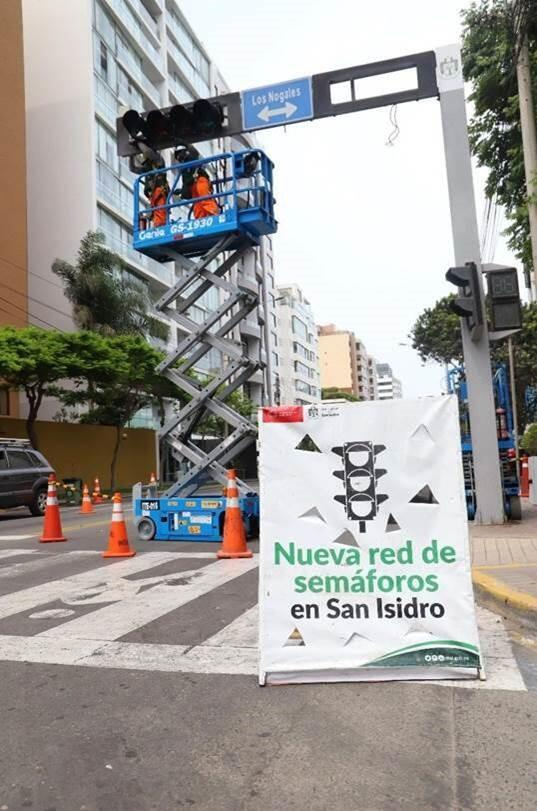
\includegraphics[width=0.92\linewidth,height=0.62\textheight,keepaspectratio]{./media/image149.png}
\captionof*{figure}{\small\itshape Figura 1. Instalación de semáforos inteligentes en San Isidro, como parte del proyecto de modernización de la red semafórica en Lima (ITS Perú, 2024).}
\addcontentsline{lof}{figure}{Figura 1. Instalación de semáforos inteligentes en San Isidro, como parte del proyecto de modernización de la red semafórica en Lima (ITS Perú, 2024).}
\label{fig:1}
\end{center}

Esto reafirma que a nivel local existe factibilidad técnica y beneficios claros al adoptar sistemas de semaforización adaptativa con tecnología moderna.

En la práctica, las ciudades inteligentes están adoptando arquitecturas híbridas donde cierta toma de decisiones ocurre localmente complementada por supervisión y coordinación global desde la nube. Con la creciente digitalización de la infraestructura vial, la seguridad cibernética se ha convertido en una preocupación primordial en los sistemas de control de tráfico. Tradicionalmente, los controladores de semáforo eran dispositivos aislados (sistemas embebidos de propósito específico) con mecanismos de comunicación propietarios. Sin embargo, al integrarlos a redes, se exponen a riesgos similares a los de cualquier dispositivo conectado. Varios estudios han revelado vulnerabilidades serias en equipos de semaforización existentes. Un caso documentado es el del controlador Intelight X-1, muy utilizado en Norteamérica, cuya interfaz web presentó vulnerabilidades, permitiendo que atacantes pudieran acceder de forma remota sin autenticación. Esta falta de medidas de seguridad dejaba el sistema expuesto a manipulaciones externas, lo que podría haber permitido a los atacantes alterar el funcionamiento de los semáforos (El Español, 2024).

\section{Descripción de la Problemática}\label{descripciuxf3n-de-la-problemuxe1tica}

\textbf{La ineficiencia del sistema semafórico de Lima para gestionar el tránsito vehicular} de manera óptima y segura es uno de los mayores desafíos urbanos que enfrenta Lima Metropolitana, afectando directamente la calidad de vida de sus habitantes. La ciudad ha alcanzado niveles alarmantes de lentitud en el tráfico, con una velocidad promedio de 14.5 km/h durante las horas punta, lo que la convierte en la más congestionada de América Latina (El Comercio, 2025). Este fenómeno no solo genera enormes pérdidas de tiempo, sino que también implica un costo económico significativo, estimado en un 1.8\% del Producto Bruto Interno (PBI) de Perú, mientras que las emisiones del tráfico representan cerca del 40\% de la contaminación urbana (Banco Mundial, 2024).

\textbf{Una de las principales causas de esta problemática es} la ineficiencia del sistema semafórico actual. La mayoría de los semáforos en Lima operan con ciclos preestablecidos, sin una adaptación al flujo vehicular en tiempo real. Este diseño rígido genera colas innecesarias en algunas intersecciones y desaprovecha otras, lo que agrava aún más la congestión (BBMLED, 2023). Además, las paradas prolongadas causadas por los semáforos fijos resultan en un aumento del consumo de combustible y una mayor emisión de contaminantes por parte de los vehículos, lo que incrementa la huella de carbono en la ciudad. Estas deficiencias en la infraestructura de control del tráfico también afectan la productividad económica, ya que los retrasos en el transporte contribuyen a la ineficiencia en los negocios y servicios. Una vista más general de la problemática se puede observar en la Figura 2.

\textbf{Las consecuencias de un sistema semafórico} obsoleto, ineficiente y no adaptativo son variadas. Entre las principales consecuencias se encuentran la congestión vehicular, la pérdida de tiempo para los conductores, y un mayor consumo energético y emisiones contaminantes. En términos de seguridad vial, la descoordinación semafórica incrementa el riesgo de accidentes, ya que los conductores, frustrados por las demoras, incurren en conductas temerarias como cruzar en ámbar o rojo, lo que aumenta la probabilidad de colisiones. Además, el sistema actual inteligente presenta serias vulnerabilidades cibernéticas.

Estos riesgos de hackeo han sido documentados en sistemas semafóricos en varias partes del mundo, y han obligado a tomar medidas drásticas, como la actualización de gran parte de las redes semafóricas en Europa, ante la vulnerabilidad de los antiguos controladores (Bitdefender, 2020; Transportation Research Board, 2023). En este contexto, el sistema semafórico actual de Lima no cumple adecuadamente su función básica de regular el tránsito de forma segura y expedita, contribuyendo a la congestión, la contaminación y poniendo en riesgo la seguridad pública.

\begin{center}
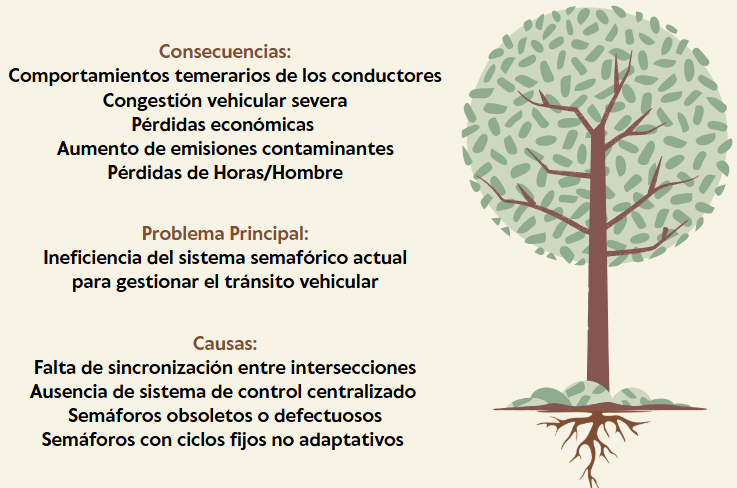
\includegraphics[width=0.92\linewidth,height=0.62\textheight,keepaspectratio]{./media/image116.png}
\captionof*{figure}{\small\itshape Figura 2. Árbol de problemas (Creación propia).}
\addcontentsline{lof}{figure}{Figura 2. Árbol de problemas (Creación propia).}
\label{fig:2}
\end{center}

\section{Propuesta de solución}\label{propuesta-de-soluciuxf3n}

Frente a la problemática identificada de la ineficiencia del sistema semafórico actual en Lima Metropolitana, que provoca congestión vehicular, pérdidas económicas, aumento del consumo energético y elevados niveles de contaminación, se propone un sistema de control adaptativo inteligente basado en tecnologías IoT (Internet de las Cosas), algoritmos de inteligencia artificial y mecanismos de comunicación en la nube con medidas de seguridad cibernética. Este sistema busca mitigar las consecuencias negativas de la infraestructura semafórica obsoleta, como los comportamientos temerarios de los conductores, la congestión vehicular, las pérdidas económicas, el aumento de las emisiones contaminantes y las pérdidas de horas/hombre.

El sistema propuesto consiste en un módulo electrónico que complementa al sistema semafórico actual, optimizando dinámicamente los ciclos semafóricos en tiempo real según la demanda vehicular en cada intersección. Este módulo estará equipado con una cámara como sensor principal de detección vehicular, proporcionando datos sobre el flujo, velocidad promedio y cola vehicular en cada dirección del cruce semafórico, como se observa en la Figura 3.

A través de sensores IoT ubicados en intersecciones críticas y el uso de APIs, el sistema recopilará datos actualizados que utilizará para calcular el índice de congestión vehicular, permitiendo una percepción precisa de las condiciones del tráfico. Además, se integrarán algoritmos de inteligencia artificial que ajustarán los tiempos semafóricos de acuerdo con el flujo detectado, optimizando los ciclos y respondiendo adaptativamente ante eventos imprevistos como accidentes o congestión inesperada.

La comunicación entre los datos recolectados de las intersecciones y la plataforma central se realizará mediante una infraestructura en la nube, proporcionando análisis global y una coordinación de red centralizada. Esto permitirá tomar decisiones basadas en datos actualizados y facilitará la supervisión remota eficaz de todas las intersecciones semafóricas de Lima Metropolitana. Además, el módulo incluirá medidas de seguridad cibernética, alineadas con los estándares internacionales.

Este sistema contribuye a mejorar la fluidez del tráfico, al reducir las demoras y el tiempo de espera en las intersecciones, lo que disminuye la congestión vehicular. Al optimizar los ciclos semafóricos, se reduce la frustración de los conductores, lo que disminuye los comportamientos temerarios y las pérdidas de tiempo y consumo de combustible. Esto, a su vez, mejora la productividad económica y reduce las emisiones contaminantes. Además, la eficiencia del sistema permite reducir las horas/hombre perdidas en el tráfico, beneficiando tanto el transporte de personas como el de mercancías, y contribuyendo a la reducción de la huella de carbono en la ciudad.

\section{Objetivos de la tesis}\label{objetivos-del-proyecto-de-tesis}

\subsection{Objetivo general}\label{objetivo-general}

Diseñar un módulo IoT de control adaptativo complementario al controlador semafórico existente, integrando visión por computadora, procesamiento local, control difuso, comunicación segura con la nube y medidas de ciberseguridad para mejorar el desempeño del flujo vehicular en intersecciones urbanas.

\subsection{Objetivos específicos}\label{objetivos-especuxedficos}

\begin{itemize}
\item
  Analizar el estado actual del sistema semafórico en Lima e identificar sus principales deficiencias, desarrollando la base conceptual del sistema propuesto.
\item
  Diseñar la arquitectura completa del sistema de control adaptativo inteligente, especificando la integración de sensores industriales, algoritmos de visión por computadora y sistemas de comunicación NTCIP/MQTT.
\item
  Desarrollar los esquemas electrónicos detallados del controlador basado en una unidad de procesamiento embebida, incluyendo módulos de entrada/salida, protecciones eléctricas, sistemas de alimentación con respaldo UPS e interfaces de comunicación.
\item
  Desarrollar y validar en simulación un esquema de control adaptativo basado principalmente en lógica difusa local, considerando módulos complementarios de optimización y predicción en la nube sin comprometer la operación segura ante pérdida de conectividad.
\item
  Diseñar un sistema de movimiento automatizado para la cámara mediante un actuador y un sistema de rieles para garantizar cobertura visual en la intersección.
\item
  Diseñar el gabinete modular mediante software CAD, realizando cálculos estructurales de resistencia mecánica y diseño del sistema de rieles externos para la cámara, asegurando resistencia a condiciones climáticas adversas y vandalismo.
\end{itemize}

\section{Alcance del trabajo}\label{alcance-del-trabajo}

El presente trabajo corresponde a una tesis de titulación enfocada en el diseño, simulación y validación en entorno controlado de un módulo IoT complementario para control semafórico adaptativo. El alcance incluye el diseño conceptual del sistema, la selección y justificación de sensores, actuadores, unidad de procesamiento, comunicaciones, arquitectura de nube, medidas de ciberseguridad, diseño electrónico, diseño mecánico, propuesta de control adaptativo y validación mediante simulación.

El sistema se plantea como una solución de apoyo al controlador semafórico existente. Por tanto, el controlador certificado de la intersección mantiene la autoridad final sobre los estados de luces, enclavamientos, fases incompatibles y modos seguros. El módulo propuesto calcula variables de tráfico, genera recomendaciones o parámetros de ajuste y comunica información hacia la nube y la central semafórica, sin sustituir los mecanismos de seguridad funcional propios del controlador vial.

El trabajo no incluye fabricación física, instalación en campo, certificación normativa, pruebas con tráfico real ni validación directa con controladores comerciales específicos. La compatibilidad con marcas y protocolos presentes en Lima se formula como una arquitectura de integración basada en interfaces estándar, pero su verificación con equipos propietarios queda fuera del alcance. Asimismo, la validación de ciberseguridad se limita al diseño de medidas, modelo de amenazas y criterios de mitigación, sin constituir una auditoría formal ni una certificación IEC 62443.

El alcance geográfico se mantiene en intersecciones representativas modeladas en simulación. La extrapolación a corredores completos o a toda la red semafórica metropolitana se considera una línea futura que requerirá calibración con datos reales, validación operacional, acuerdos institucionales y pruebas piloto progresivas.

\section{Metodología empleada}\label{metodologuxeda-empleada}

Para el desarrollo de la tesis se emplea la metodología VDI 2221 como marco principal de diseño sistemático, complementada con VDI 2206 para ordenar la integración mecatrónica entre mecánica, electrónica, control e informática. Design Thinking se utiliza únicamente como apoyo en la etapa inicial de identificación de necesidades de usuarios, operadores e instituciones vinculadas a la gestión del tránsito.

La metodología VDI 2221 guía el proceso desde la clarificación de la tarea hasta el diseño conceptual, la selección de alternativas y el desarrollo detallado. En primer lugar, se identifica la problemática de congestión vial y se definen los objetivos, el alcance y los requerimientos del sistema. Luego se revisa el estado del arte en sensado vehicular, control adaptativo, comunicaciones IoT, ciberseguridad y simulación de tráfico. A partir de esa revisión se construye la estructura de funciones, se plantean alternativas de solución y se selecciona una solución óptima mediante evaluación técnica y económica.

VDI 2206 se incorpora en las etapas de integración del sistema mecatrónico, donde se relacionan el diseño mecánico del gabinete y soporte, el diseño electrónico de alimentación y procesamiento, el algoritmo de control, la comunicación con la nube y la validación mediante simulación. Este enfoque permite verificar que las decisiones de diseño no se analicen de forma aislada, sino como parte de una arquitectura completa y coherente.

Luego de ello, se define la lista de requerimientos, explicando cada parámetro como deseo o exigencia. De igual forma, se realiza la matriz morfológica con las múltiples soluciones encontradas en el estado del arte, según la estructura de funciones. Con ello, mediante una evaluación técnica-económica (usando criterios ponderados como costo, complejidad, eficiencia y compatibilidad), se determina la solución óptima. Para el desarrollo técnico, se inicia describiendo la arquitectura general del sistema, incluyendo bloques funcionales para entradas/salidas, procesamiento y comunicaciones (NTCIP/TCP-IP y MQTT).

Además, es necesario contar con la arquitectura para diseñar un sistema de control adaptativo y su posterior simulación en herramientas como SUMO (para tráfico) y MATLAB-Simulink (para algoritmos). Asimismo, se eligen sensores específicos y actuadores necesarios para el controlador. A medida que se avanza con el trabajo, se diseña el modelo 3D, calculando distribución de componentes, centro de masa y análisis térmico para garantizar ventilación adecuada y resistencia estructural en entornos urbanos. Por consiguiente, se realiza la prueba de resistencia del gabinete, evaluando zonas críticas de esfuerzo bajo cargas de vandalismo, humedad o vibraciones. Luego de ello, se buscan arquitecturas para el algoritmo de visión por computadora que detecta vehículos, emergencias y colas en tiempo real, escogiendo la más óptima en base a métricas probadas con datasets de imágenes urbanas.

Posteriormente, se diseña la infraestructura en Azure, incluyendo IoT Hub para telemetría, Stream Analytics para procesamiento y SQL Database para logs históricos, integrando API de Google Maps y medidas de ciberseguridad. Se desarrolla la interfaz de usuario local y remota (dashboard en Azure) para supervisar estados: métricas de tráfico, alertas, batería UPS, etc.

Terminando, se realizan los esquemas electrónicos detallados, que especifican conexiones entre elementos. Se elaboran los planos de ensamble, visualizando la integración modular de componentes mecánicos y electrónicos, junto con validaciones finales mediante prototipos simulados.

\chapter{ESTADO DE LAS TECNOLOGÍAS}\label{capuxedtulo-2-estado-de-las-tecnologuxedas}

En este capítulo se presenta una revisión del estado del arte. Se abordan las tecnologías y dispositivos involucrados (sensores, actuadores y controladores), los enfoques de control adaptativo existentes, la integración de sistemas IoT y comunicaciones en la nube, las normativas y estándares relevantes, las soluciones comerciales vigentes, los principales aportes de la literatura académica reciente, y las herramientas de simulación de tráfico disponibles. Cada sección concluye con las lecciones clave que aporta al diseño conceptual propuesto de un módulo IoT para control adaptativo de semáforos.

\section{Tecnologías de sensado vehicular y actuadores en sistemas de tráfico}\label{tecnologuxedas-de-sensado-vehicular-y-actuadores-en-sistemas-de-truxe1fico}

Un sistema semafórico inteligente depende de la detección fiable del flujo vehicular y de actuadores eficientes para gestionar las señales luminosas del semáforo. La detección de vehículos en intersecciones tradicionalmente se ha realizado mediante sensores empotrados en la vía, como los lazos inductivos. Un lazo inductivo consiste en un bucle de cable instalado bajo el pavimento que funciona como un detector magnético al paso de un vehículo (una masa metálica). Este vehículo altera la inductancia, lo que permite detectar la presencia o paso de vehículos (Buchanan, 2023).

Estos sensores han sido el sistema de detección tradicional de muchos sistemas de tráfico debido a su precisión y tiempo de respuesta. Sin embargo, presentan desventajas en cuanto a costes de instalación y mantenimiento, ya que requieren obras en la calzada y pueden dañarse con el tiempo o durante repavimentaciones. En la última década se han incorporado sensores sobre la superficie como cámaras de vídeo, radares de microondas y magnetómetros inalámbricos para complementar o reemplazar a los lazos. Un ejemplo de sistema que utiliza lazos inductivos se puede ver en la Figura 3.

\begin{center}
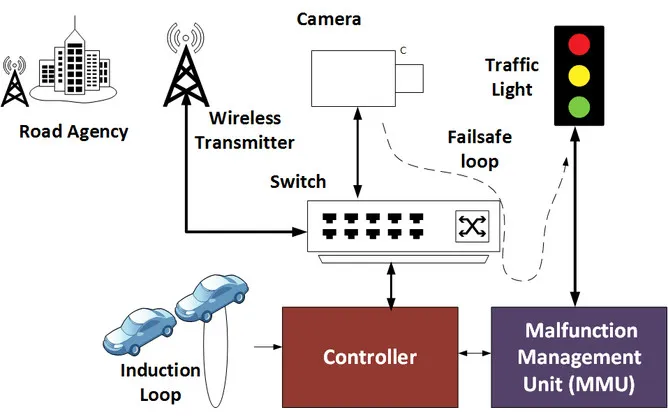
\includegraphics[width=0.92\linewidth,height=0.62\textheight,keepaspectratio]{./media/image25.png}
\captionof*{figure}{\small\itshape Figura 3. Vista general de un sistema de control de tráfico (Buchanan, 2023).}
\addcontentsline{lof}{figure}{Figura 3. Vista general de un sistema de control de tráfico (Buchanan, 2023).}
\label{fig:3}
\end{center}

Las cámaras permiten una detección más flexible (identificando varios carriles, peatones, incluso clasificando tipos de vehículos) y son utilizados también como vigilancia de infracciones, no obstante, su desempeño puede degradarse con condiciones climáticas adversas como las presentes en Lima (humedad relativa alta, polvo en el ambiente) o como problemas más generales como iluminación deficiente, y requieren algoritmos de visión artificial para interpretar la imagen. Los sensores radar de microondas, instalados típicamente sobre el semáforo, emiten ondas y miden su reflejo para detectar vehículos y estimar su velocidad, operan bien de día y noche y bajo lluvia, aunque pueden ser costosos rondando precios de los miles de soles. Por otro lado, se han implementado magnetómetros inalámbricos (pequeños sensores enterrados o superficiales alimentados por batería) que detectan cambios en el campo magnético terrestre producidos por vehículos; estos sensores, a menudo conectados en red inalámbrica, facilitan la instalación (sin tendido de cables) y la cobertura modular de múltiples puntos en la intersección\hspace{0pt} (Gheorghe y Soica, 2025).

En cuanto a los actuadores del sistema de tráfico, los principales son las luces (rojo, ámbar, verde). Históricamente, las lámparas incandescentes fueron usadas en semáforos, pero actualmente casi todos los semáforos modernos emplean tecnología LED. Las luces LED ofrecen mayor eficiencia energética (consumen hasta un 80-90\% menos electricidad), mayor vida útil (del orden de 50,000 horas, reduciendo costos de reemplazo) y mejor visibilidad (intensidad luminosa alta y colores más nítidos). Además, los módulos LED permiten incluir diodos redundantes de forma que si falla uno, el aspecto sigue siendo visible parcialmente, mejorando la seguridad\hspace{0pt} \emph{(Buchanan, 2023).\\
}

Los actuadores también incluyen los controladores de corriente que encienden/apagan las luces siguiendo las órdenes lógicas del controlador principal; estos deben cumplir normas de seguridad para evitar estados peligrosos como omitir una sección de luz. Además, se destaca la presencia de unidades de monitoreo de malfuncionamiento (\emph{Malfunction Management Units}, MMU) en los gabinetes de control, las cuales fuerzan al semáforo a un estado de flashing (intermitencia) de seguridad (típicamente parpadeo amarillo) si se detecta alguna inconsistencia o fallo en la secuencia de luces. \emph{(Buchanan, 2023).}

Otro elemento de sensado importante son los dispositivos para detección de demanda peatonal, como botones de pulsación para peatones o sensores infrarrojos que detectan personas esperando para cruzar. Estos alimentan al controlador con información sobre la presencia de peatones y la necesidad de servicio de fase peatonal. Imagen referencial en la Figura 4.

\begin{center}
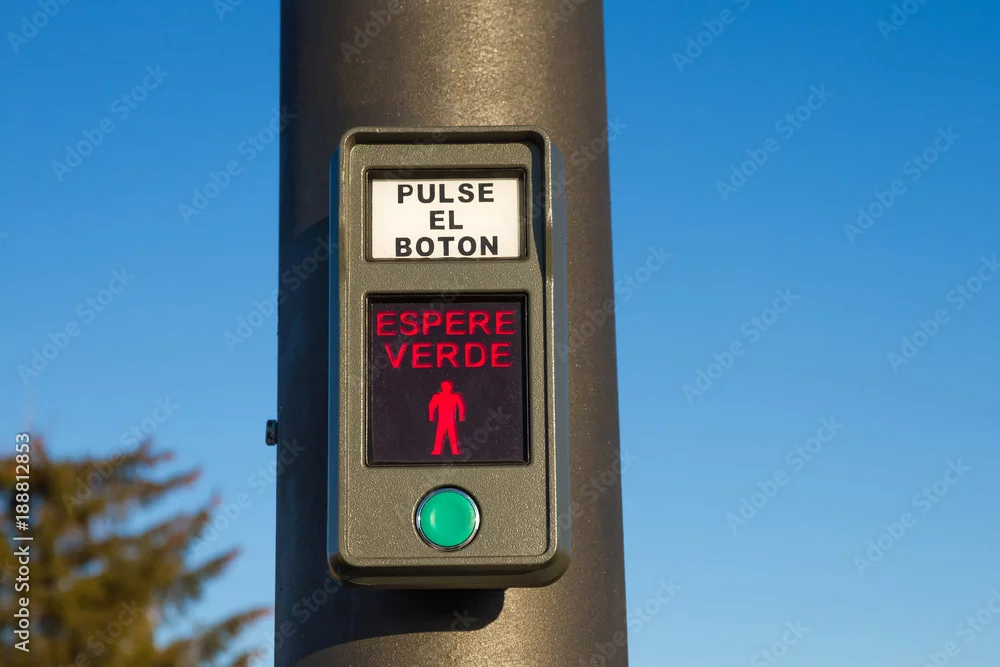
\includegraphics[width=0.92\linewidth,height=0.62\textheight,keepaspectratio]{./media/image47.png}
\captionof*{figure}{\small\itshape Figura 4. Botón pulsador para solicitar paso de peatones en un semáforo. Fuente: Adobe Stock}
\addcontentsline{lof}{figure}{Figura 4. Botón pulsador para solicitar paso de peatones en un semáforo. Fuente: Adobe Stock}
\label{fig:4}
\end{center}

\Needspace{6\baselineskip}
\captionof*{table}{\small\bfseries Tabla 2.1. Comparativa de tecnologías de detección de vehículos en intersecciones. (Creación propia).}
\addcontentsline{lot}{table}{Tabla 2.1. Comparativa de tecnologías de detección de vehículos en intersecciones. (Creación propia).}
\label{tbl:2.1}

\begin{longtable}[]{@{}
  >{\raggedright\arraybackslash}p{(\columnwidth - 8\tabcolsep) * \real{0.2000}}
  >{\raggedright\arraybackslash}p{(\columnwidth - 8\tabcolsep) * \real{0.2000}}
  >{\raggedright\arraybackslash}p{(\columnwidth - 8\tabcolsep) * \real{0.2000}}
  >{\raggedright\arraybackslash}p{(\columnwidth - 8\tabcolsep) * \real{0.2000}}
  >{\raggedright\arraybackslash}p{(\columnwidth - 8\tabcolsep) * \real{0.2000}}@{}}
\toprule
\begin{minipage}[b]{\linewidth}\raggedright
\textbf{Tecnología de sensor}
\end{minipage} & \begin{minipage}[b]{\linewidth}\raggedright
\textbf{Principio de funcionamiento}
\end{minipage} & \begin{minipage}[b]{\linewidth}\raggedright
\textbf{Ventajas principales}
\end{minipage} & \begin{minipage}[b]{\linewidth}\raggedright
\textbf{Limitaciones / Desventajas}
\end{minipage} & \begin{minipage}[b]{\linewidth}\raggedright
\textbf{Aplicaciones típicas}
\end{minipage} \\
\begin{minipage}[b]{\linewidth}\raggedright
Lazo inductivo
\end{minipage} & \begin{minipage}[b]{\linewidth}\raggedright
Inductancia alterada por vehículo
\end{minipage} & \begin{minipage}[b]{\linewidth}\raggedright
Alta precisión, Respuesta inmediata
\end{minipage} & \begin{minipage}[b]{\linewidth}\raggedright
Instalación invasiva, Mantenimiento
\end{minipage} & \begin{minipage}[b]{\linewidth}\raggedright
Detectar presencia por carril
\end{minipage} \\
\begin{minipage}[b]{\linewidth}\raggedright
Cámara de video
\end{minipage} & \begin{minipage}[b]{\linewidth}\raggedright
Visión artificial
\end{minipage} & \begin{minipage}[b]{\linewidth}\raggedright
Cobertura amplia, Clasificación visual
\end{minipage} & \begin{minipage}[b]{\linewidth}\raggedright
Sensible a clima/iluminación, Procesamiento intensivo
\end{minipage} & \begin{minipage}[b]{\linewidth}\raggedright
Conteo y clasificación, Detección de infracción
\end{minipage} \\
\begin{minipage}[b]{\linewidth}\raggedright
Sensor radar
\end{minipage} & \begin{minipage}[b]{\linewidth}\raggedright
Microondas refleja en vehículo
\end{minipage} & \begin{minipage}[b]{\linewidth}\raggedright
Funciona 24h y con mal clima, mide velocidad
\end{minipage} & \begin{minipage}[b]{\linewidth}\raggedright
Costo relativamente alto, Cobertura focal
\end{minipage} & \begin{minipage}[b]{\linewidth}\raggedright
Detección de aproximación, Velocidades en vía
\end{minipage} \\
\begin{minipage}[b]{\linewidth}\raggedright
Magnetómetro inalámbrico
\end{minipage} & \begin{minipage}[b]{\linewidth}\raggedright
Campo magnético terrestre
\end{minipage} & \begin{minipage}[b]{\linewidth}\raggedright
Fácil instalación, Malla inalámbrica flexible
\end{minipage} & \begin{minipage}[b]{\linewidth}\raggedright
Alcance limitado, Vida de batería finita
\end{minipage} & \begin{minipage}[b]{\linewidth}\raggedright
Presencia en puntos específicos, apoyo a lazos
\end{minipage} \\
\begin{minipage}[b]{\linewidth}\raggedright
Otros (ultrasonido, IR, etc.)
\end{minipage} & \begin{minipage}[b]{\linewidth}\raggedright
Ondas ultrasónicas o infrarrojas
\end{minipage} & \begin{minipage}[b]{\linewidth}\raggedright
Bajo costo
\end{minipage} & \begin{minipage}[b]{\linewidth}\raggedright
Alcance corto, Afectados por ambiente
\end{minipage} & \begin{minipage}[b]{\linewidth}\raggedright
Uso experimental o complementario
\end{minipage} \\
\midrule
\endhead
\bottomrule
\endlastfoot
\end{longtable}

En resumen, las tecnologías de sensado vehicular han evolucionado para proporcionar datos cada vez más confiables sobre el flujo de tráfico, mientras que los actuadores (luces LED) garantizan una señalización más eficiente y segura. Para el diseño conceptual de un módulo IoT adaptativo, esto sugiere la conveniencia de combinar múltiples fuentes de detección a fin de obtener una imagen integral del tránsito en tiempo real. Asimismo, se deberá asegurar que el módulo pueda accionar los semáforos de forma fiable y segura, aprovechando las ventajas de las luces LED y cumpliendo mecanismos de failsafe. La selección de sensores se seguirá en función de equilibrar costo, facilidad de despliegue e interoperabilidad, teniendo en mente que la infraestructura existente puede integrarse en la solución IoT para reducir costos y aprovechar los datos.

\section{Controladores de tráfico}\label{controladores-de-truxe1fico}

El controlador de tráfico es el dispositivo lógico (normalmente una unidad electrónica programable instalada en un gabinete junto a la intersección) que recibe la información de los sensores y ejecuta la lógica de temporización de las luces. En sistemas convencionales, estos controladores operan en base a planes fijos de tiempos de verde por fase o mediante esquemas de control actuado donde cada fase (Color brillante) del semáforo se activa sólo cuando un detector indica demanda (vehículos o peatones presentes), y la duración de verde puede extenderse dinámicamente hasta un máximo predefinido mientras siga habiendo vehículos detectados en esa aproximación. Este enfoque mejora la eficiencia respecto a planes fijos, pero está limitado a la optimización local de cada intersección.

Actualmente en el Perú los controladores semafóricos están encargado de controlar un conjunto de semáforos y equipos periféricos en la intersección donde fueron instalados. Estos controladores tienen la capacidad de manejar hasta 20 fases semafóricas, lo que significa que pueden coordinar 20 configuraciones diferentes de luces para regular el paso vehicular y peatonal en distintas direcciones o movimientos, lo que lo vuelve más adaptable en intersecciones complejas, tan presentes en Lima. Además, estos controladores pueden sub - regular hasta 4 intersecciones lo que implica que tiene la capacidad de supervisar y coordinar el funcionamiento de semáforos en cuatro intersecciones cercanas. Estos dispositivos están diseñados para integrarse a una plataforma de Gestión de tránsito, por lo que son capaces de conectarse a la Gerencia de Movilidad Urbana, específicamente de la Subgerencia de Gestión y Fiscalización de la Municipalidad de Lima, pues desde la Ordenanza N°2537 este organismo es el responsable de optimizar los sistemas de gestión y control de tránsito, mejorar la movilidad y garantizar un adecuado control y mantenimiento de los sistemas relacionados al transporte (ITS Perú, 2024). En la figura 6 se observa la central semafórica de Lima.

\begin{center}
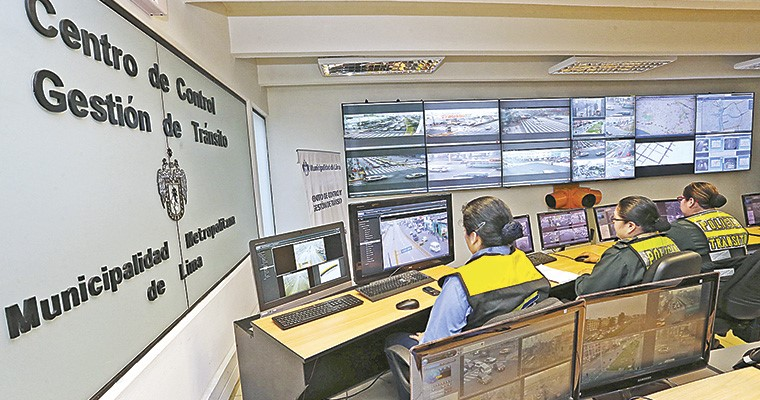
\includegraphics[width=0.92\linewidth,height=0.62\textheight,keepaspectratio]{./media/image17.png}
\captionof*{figure}{\small\itshape Figura 5. Centro de control Gestión de tránsito de la Municipalidad Metropolitana de Lima\\}
\addcontentsline{lof}{figure}{Figura 5. Centro de control Gestión de tránsito de la Municipalidad Metropolitana de Lima\\}
\label{fig:5}
\end{center}

En el distrito de San Isidro, se ha implementado un sistema moderno con el controlador TEK UTC-3, de origen alemán, reconocido por cumplir estándares europeos de control de tráfico inteligente. Este dispositivo, instalado en gabinetes robustos en vía pública, destaca por su diseño modular, capacidad de operación en red y alta compatibilidad con sensores y plataformas de gestión de tránsito (ITS Perú, 2024).

El ITC-3 es un controlador modular programable (PLC embebido) diseñado para operar en entornos urbanos complejos con capacidad de hasta 32 fases semafóricas y múltiples entradas/salidas digitales y analógicas. Integra una pantalla táctil HMI para configuración in situ y diagnóstico, y permite ejecutar algoritmos de control adaptativo en tiempo real que ajustan la duración de las fases de acuerdo al volumen vehicular detectado por sensores. Soporta comunicación redundante vía Ethernet, fibra óptica y módem celular bajo protocolos TCP/IP y NTCIP, garantizando alta disponibilidad y capacidad de integración con plataformas superiores de gestión (ITS Perú, 2024).

El sistema en San Isidro se encuentra enlazado al Centro de Control de Tránsito Distrital, donde opera el software OMNIA, también de SWARCO, que permite una supervisión centralizada, análisis de datos históricos y programación remota de planes semafóricos. Su implementación ha permitido en San Isidro una gestión más eficiente del flujo vehicular, reducción de tiempos de espera y mejor respuesta ante la variabilidad del tráfico urbano. En la Figura 7 se muestra uno de estos controladores instalado, según ITS Perú (2024).

\begin{center}
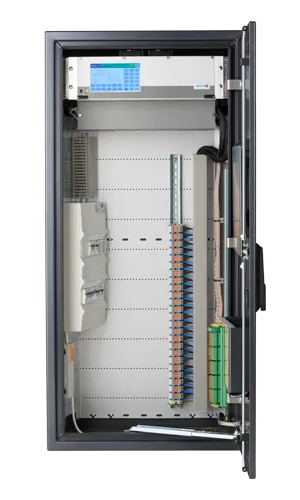
\includegraphics[width=0.92\linewidth,height=0.62\textheight,keepaspectratio]{./media/image43.png}
\captionof*{figure}{\small\itshape Figura 6. Controlador ITC-3 de la marca austriaca SWARCO TECHNOLOGY APS. Fuente: TEK Perú,}
\addcontentsline{lof}{figure}{Figura 6. Controlador ITC-3 de la marca austriaca SWARCO TECHNOLOGY APS. Fuente: TEK Perú,}
\label{fig:6}
\end{center}

En la actualidad, los avances en electrónica y comunicaciones han posibilitado controladores mucho más sofisticados, capaces de conectarse en red y adaptarse en tiempo real a las condiciones de tráfico. Los sistemas de control de tráfico adaptativo son capaces de modificar continuamente los parámetros de temporización (longitud de ciclos, distribuciones de tiempos de verde por fase, offsets de coordinación entre semáforos consecutivos, etc.) en respuesta a la demanda observada. Ejemplos destacados de algoritmos adaptativos tradicionales son SCOOT (Siglas de \emph{Split Cycle Offset Optimization Technique}) desarrollado en el Reino Unido y SCATS (\emph{Sydney Coordinated Adaptive Traffic System}) desarrollado en Australia. Ambos sistemas ajustan los intervalos de los semáforos de manera cíclica.

SCATS ajusta continuamente el ciclo y la división de tiempos midiendo la saturación en la línea de parada y los volúmenes vehiculares en las aproximaciones\hspace{0pt} (Fehon, 2016).

SCOOT, por su parte, realiza pequeñas correcciones en cada ciclo de semáforo basándose en detectores upstream (antes de la intersección) que miden la congestión aproximándose, optimizando así los \emph{offsets} (desfases) entre intersecciones para crear ``olas verdes'' progresivas. Estos sistemas suelen operar de forma centralizada, un computador central recibe datos de las intersecciones y calcula los ajustes coordinados en un área urbana. Han demostrado eficacia en la reducción de demoras e incremento de capacidad en entornos urbanos, aunque requieren una calibración cuidadosa y conllevan una inversión considerable en infraestructura de detección y comunicación\hspace{0pt}. En contraste, han emergido enfoques novedosos de control descentralizado. Por ejemplo, el sistema Surtrac (\emph{Scalable Urban Traffic Control}), surgido de la academia, propone que cada intersección (o un agente en cada controlador) tome decisiones localmente de forma asíncrona, comunicándose sólo con intersecciones vecinas para intercambiar información de flujos futuros\hspace{0pt} (Smith, Barlow, Xie, \& Rubinstein, 2013). Surtrac asigna el verde en cada ciclo de manera independiente, basado en colas detectadas y tiempos de llegada previstos, y luego envía a los próximos semáforos una proyección de su flujo de salida para lograr cierta coordinación distribuida\hspace{0pt} (Smith, Barlow, Xie, \& Rubinstein, 2013). Este diseño \emph{multi-agent} descentralizado busca mejorar la escalabilidad (se pueden añadir intersecciones sin reconfigurar un centro de control) y la robustez ante fallos de comunicación (si se pierde conexión, cada semáforo sigue operando localmente) (Smith, Barlow, Xie, \& Rubinstein, 2013).

Surtrac logró reducciones significativas de tiempos de viaje y demoras en pruebas de campo en Pittsburgh\hspace{0pt}, mostrando el potencial de estos esquemas.

Muchos de los sistemas de control de tráfico cumplen estándares como los controladores tipo ATC (Advanced Transportation Controller) o los estándares de la NEMA (National Electrical Manufacturers Association) en EE.UU., los cuales definen arquitectura modular de hardware y protocolos de comunicación estandarizados. Un controlador moderno típicamente es un sistema embebido robusto, con capacidad de ejecutar múltiples planes, algoritmos adaptativos y comunicación de datos (Ethernet, módem celular, fibra óptica, etc.), todo dentro de un gabinete en la calle. Estos controladores incorporan interfaces para conectar detectores (entradas) y cabezas de semáforo (salidas a relés o drivers electrónicos para luces LED), además de puertos de comunicación para enlaces a un centro de control o a otros controladores. Dado que mi sistema propuesto involucra IoT y comunicación en la nube, es relevante destacar que muchos controladores recientes ya utilizan protocolos de red (TCP/IP) para reportar datos y recibir comandos. Por ejemplo, SCATS emplea comunicación TCP/IP con aproximadamente 8 kB/s por controlador, interrogando a cada controlador una vez por segundo desde el centro\hspace{0pt} (Tario \& Dillmann, 2014)

Los mecanismos de control adaptativo actuales demuestran que es posible optimizar dinámicamente la operación de redes semafóricas, ya sea mediante estrategias centralizadas o descentralizadas. Para el diseño del módulo IoT propuesto, se deriva que una arquitectura híbrida podría aprovechar ventajas de ambos enfoques: por ejemplo, procesar datos localmente en cada intersección (inteligencia en el borde) asegurando respuesta rápida, y a la vez comunicar información al nivel de nube para coordinar múltiples intersecciones y obtener una optimización global del corredor vial. Asimismo, el módulo IoT diseñado debe ser compatible con la infraestructura existente e integrarse a controladores de tráfico estándares mediante protocolos comunes, sin sustituir sus funciones críticas de seguridad funcional. La sección destaca además la importancia de incorporar algoritmos adaptativos inteligentes como herramientas de apoyo para superar las limitaciones de los sistemas tradicionales.

\section{Integración de sistemas IoT y comunicación en la nube en semáforos}\label{integraciuxf3n-de-sistemas-iot-y-comunicaciuxf3n-en-la-nube-en-semuxe1foros}

La incorporación de la Internet de las Cosas (IoT) en sistemas de control de tráfico ha abierto nuevas posibilidades para la conectividad y gestión remota de semáforos. Un sistema de semáforos inteligente habilitado para IoT típicamente consta de dispositivos o módulos conectados a cada controlador o semáforo que pueden sensar el entorno, comunicarse inalámbricamente y ser gestionados desde plataformas en la nube.

La comunicación con la nube permite que datos en tiempo real (conteos de vehículos, estados de semáforo, fallos, etc.) sean enviados a servidores centralizados donde se pueden aplicar algoritmos más intensivos de análisis, optimización o almacenamiento histórico. A su vez, desde la nube se pueden desplegar recomendaciones, parámetros o configuraciones previamente validadas hacia la central semafórica y los módulos IoT.

Un aspecto crítico al diseñar esta integración es garantizar la baja latencia en las comunicaciones cuando se requiere control en tiempo real. Tecnologías como MQTT (Message Queuing Telemetry Transport) se emplean a menudo en IoT por su ligereza y eficiencia en entornos de ancho de banda limitado, pudiendo ser una opción para transmitir datos semafóricos. No obstante, en corredores urbanos ocupados, la latencia de enviar datos a un servidor remoto y devolver decisiones podría impactar la respuesta del semáforo. Por ello, se están explorando arquitecturas de computación en el borde (edge computing), donde parte de la inteligencia se resuelve localmente en el dispositivo IoT o el controlador de la intersección, mientras que la nube se utiliza para cálculos de mayor nivel como optimizar planes de coordinación cada tipo especificado, y para supervisión global. (Gheorghe y Soica, 2025).

Un beneficio, también relevante, de la conectividad IoT es la posibilidad de integrar datos de fuentes externas al sistema semafórico. Por ejemplo, vehículos conectados (V2I, \emph{vehicle-to-infrastructure}) pueden enviar mensajes al semáforo indicando su posición y velocidad, permitiendo una detección virtual más allá de los sensores fijos. Ya en 2010 se propuso un sistema de semáforos en red que se comunicaban con vehículos cercanos para mejorar la eficiencia en Reino unido \emph{(Asad, Saxena \& Katos, 2020)}. Actualmente, con el despliegue de tecnologías como C-V2X (Cellular Vehicle-to-Everything), es factible que los semáforos reciban información anticipada de llegada de vehículos, integrándose esto al control adaptativo. La plataforma en la nube puede servir como concentrador de estos datos V2X, agregando información de múltiples vehículos y enviando órdenes coordinadas a los semáforos. En el artículo publicado por Gheorghe y Soica se menciona que la integración de sensores IoT, comunicación V2X y algoritmos de IA puede reducir las demoras hasta en un 30\% en promedio, a la vez que mejorar índices de seguridad en el tráfico urbano\hspace{0pt}. Esto subraya la importancia de un diseño que contemple la interoperabilidad con vehículos conectados y otros dispositivos urbanos como sensores.

En la Figura 9 se representan los componentes clave que conforman un sistema de control de tráfico adaptativo moderno, donde se destacan los elementos de inteligencia artificial, infraestructura IoT, vehículos conectados, monitoreo de rendimiento y analítica predictiva. Estos elementos interactúan dinámicamente para ajustar en tiempo real los tiempos semafóricos, optimizar flujos vehiculares y mejorar la respuesta ante eventos e incidentes viales. La arquitectura representada refleja la integración de tecnologías V2I (Vehicle-to-Infrastructure), ya que contempla el intercambio de información entre vehículos y la infraestructura vial, como sensores o semáforos inteligentes, lo que permite decisiones descentralizadas, respuesta priorizada para vehículos de emergencia y una mejora global en la movilidad urbana.

\begin{center}
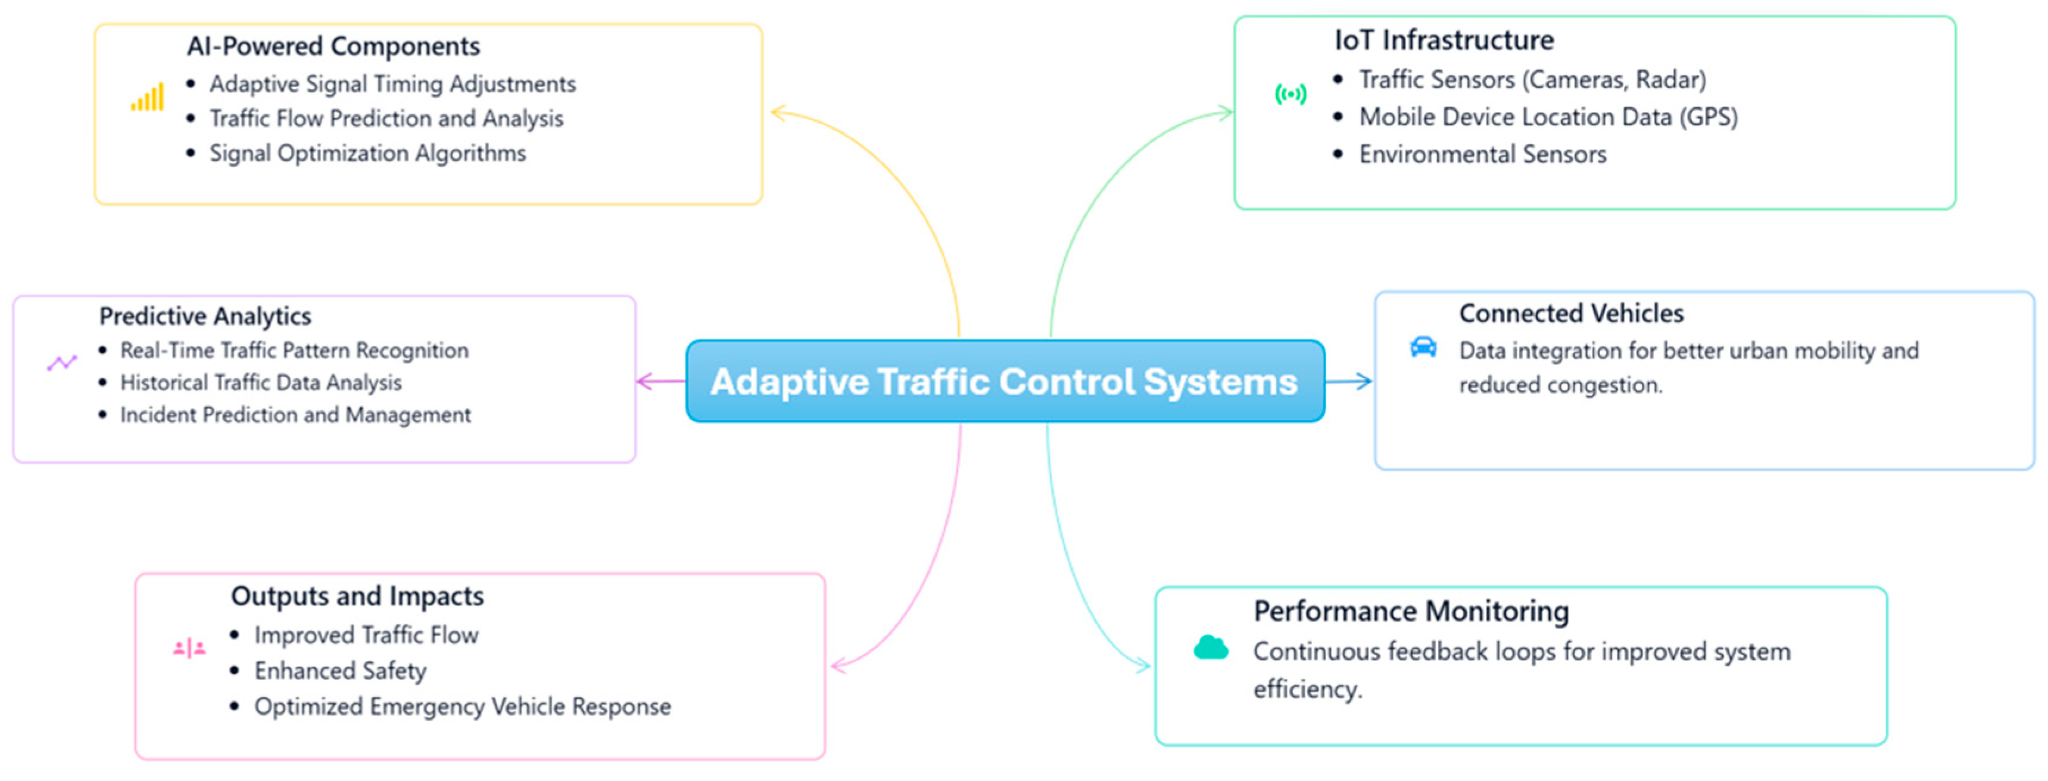
\includegraphics[width=0.92\linewidth,height=0.62\textheight,keepaspectratio]{./media/image82.png}
\captionof*{figure}{\small\itshape Figura 7. Componentes funcionales de un sistema de control de tráfico adaptativo inteligente basado en IoT e inteligencia artificial (Gheorghe y Soica, 2025).}
\addcontentsline{lof}{figure}{Figura 7. Componentes funcionales de un sistema de control de tráfico adaptativo inteligente basado en IoT e inteligencia artificial (Gheorghe y Soica, 2025).}
\label{fig:7}
\end{center}

Sin embargo, la comunicación ubicua de los semáforos con la nube y otros dispositivos conlleva riesgos de seguridad cibernética, tema que se aborda con detalle en la siguiente sección (2.5). Basta mencionar aquí que el módulo IoT debe implementar mecanismos de autenticación, cifrado de datos y control de acceso para prevenir intrusiones. Un ejemplo proveniente de los Países Bajos, es una investigación desarrollada en 2020 donde demostraron que podían manipular remotamente semáforos IoT diseñados para dar prioridad a ciclistas, enviando datos falsos que simulaban bicicletas inexistentes y logrando con ello cambiar las luces a su favor\hl{\hspace{0pt}} \emph{(Buchanan, 2023).} La ausencia de autenticación robusta en la comunicación entre la app móvil del ciclista y el semáforo permitió esta intrusión\hspace{0pt} (Kirk, 2020), no obstante esto también podría ser utilizado a favor de la central semafórica para controlar el sistema introduciendo datos adicionales.

Por lo tanto, el diseño IoT debe tomar en cuenta tales probabilidades de ataque y aplicar estándares y normas de seguridad (ver sección 2.4) para garantizar que solo entidades legítimas influyan en la operación semafórica.

Por lo ya mencionado se establece que la integración IoT y el uso de la nube en sistemas semafóricos ofrece gran potencial para mejorar la adaptabilidad y coordinación del tráfico. Para el diseño propuesto, esto implica que el módulo IoT debe actuar como un puente seguro entre el nivel local y la nube, habilitando tanto decisiones locales inmediatas como el envío de información agregada para optimización global. Las lecciones aprendidas enfatizan la necesidad de diseñar una arquitectura escalable y tolerante a fallos de comunicación, el semáforo debe poder funcionar de forma segura incluso si pierde conexión a la nube (gracias a la inteligencia local), pero aprovechará esa conexión cuando esté disponible para mejorar su desempeño con información global.

\section{Protocolos de comunicación en sistemas de tráfico}\label{protocolos-de-comunicaciuxf3n-en-sistemas-de-truxe1fico}

La comunicación efectiva entre los diferentes componentes de un sistema de control de tráfico inteligente es fundamental para su correcto funcionamiento. Los protocolos de comunicación definen las reglas y estándares que permiten el intercambio de información entre semáforos, controladores, centros de gestión y vehículos conectados. En los sistemas modernos de gestión de tráfico, la selección adecuada del protocolo de comunicación puede impactar significativamente en la latencia, confiabilidad y escalabilidad del sistema completo.

El estándar NTCIP (National Transportation Communications for ITS Protocol) se ha establecido como el protocolo dominante en América del Norte para la comunicación entre dispositivos de campo y centros de gestión. Este protocolo, desarrollado por AASHTO, ITE y NEMA, define una arquitectura de cinco capas que permite la interoperabilidad entre equipos de diferentes fabricantes. Según estudios recientes, NTCIP puede manejar hasta 10 solicitudes de prioridad simultáneas por intersección con latencias inferiores a 500 ms (NTCIP, 2025). La implementación del estándar NTCIP 1202 para controladores de señales actuadas ha sido particularmente exitosa, con más del 80\% de los controladores modernos en Estados Unidos soportando este protocolo.

Por otro lado, el protocolo UTMC (Urban Traffic Management and Control), ampliamente utilizado en Reino Unido y partes de Europa, ofrece un enfoque modular basado en estándares abiertos. UTMC permite la integración de múltiples subsistemas incluyendo CCTV, señalización variable y gestión de estacionamientos a través de una arquitectura común basada en TCP/IP. La implementación en el sistema Tees Valley ha demostrado que UTMC puede coordinar eficientemente más de 200 intersecciones con una disponibilidad del sistema superior al 99.5\% (Tees Valley Council, 2024).

En el contexto de la comunicación vehicular, los protocolos V2X (Vehicle-to-Everything) están revolucionando la manera en que los vehículos interactúan con la infraestructura vial. El estándar IEEE 802.11p, base del protocolo WAVE (Wireless Access in Vehicular Environments), opera en la banda de 5.9 GHz y proporciona comunicación de baja latencia (típicamente 10-50ms) para aplicaciones críticas de seguridad. Sin embargo, la tecnología C-V2X (Cellular Vehicle-to-Everything) está ganando tracción rápidamente, ofreciendo un 20\% mejor rendimiento en entrega de paquetes bajo condiciones de alta congestión comparado con DSRC tradicional (Chen et al., 2024).

Para la integración de dispositivos IoT en sistemas semafóricos, los protocolos ligeros como MQTT (Message Queuing Telemetry Transport) y CoAP (Constrained Application Protocol) se han vuelto esenciales. MQTT, con su arquitectura publish-subscribe y overhead mínimo de 2 bytes en el header, es ideal para la transmisión de datos de sensores con actualizaciones frecuentes. Investigaciones recientes muestran que MQTT puede lograr una confiabilidad del 99.9\% en la entrega de mensajes con QoS nivel 1, mientras mantiene latencias promedio entre 50-200 ms en redes urbanas típicas (Rahman et al., 2023). CoAP, por su parte, optimizado para dispositivos con restricciones energéticas, puede extender la vida útil de las baterías de sensores en un 30-40\% comparado con MQTT, aunque con menor throughput máximo.

La implementación práctica de estos protocolos en ciudades inteligentes ha demostrado resultados significativos. Barcelona, por ejemplo, utiliza una combinación de MQTT para telemetría de sensores IoT y protocolos HTTP/HTTPS para servicios web, logrando una integración exitosa de más de 20,000 sensores urbanos. Su plataforma Sentilo actúa como middleware horizontal, permitiendo la interoperabilidad entre diferentes protocolos y fabricantes (Barcelona Smart City, 2024).

\Needspace{6\baselineskip}
\captionof*{table}{\small\bfseries Tabla 2.2. Comparativa de protocolos de comunicación en sistemas de tráfico (Creación propia).}
\addcontentsline{lot}{table}{Tabla 2.2. Comparativa de protocolos de comunicación en sistemas de tráfico (Creación propia).}
\label{tbl:2.2}

\begin{longtable}[]{@{}
  >{\raggedright\arraybackslash}p{(\columnwidth - 10\tabcolsep) * \real{0.1503}}
  >{\raggedright\arraybackslash}p{(\columnwidth - 10\tabcolsep) * \real{0.1392}}
  >{\raggedright\arraybackslash}p{(\columnwidth - 10\tabcolsep) * \real{0.1677}}
  >{\raggedright\arraybackslash}p{(\columnwidth - 10\tabcolsep) * \real{0.1440}}
  >{\raggedright\arraybackslash}p{(\columnwidth - 10\tabcolsep) * \real{0.1867}}
  >{\raggedright\arraybackslash}p{(\columnwidth - 10\tabcolsep) * \real{0.2120}}@{}}
\toprule
\begin{minipage}[b]{\linewidth}\raggedright
\textbf{Protocolo}
\end{minipage} & \begin{minipage}[b]{\linewidth}\raggedright
\textbf{Latencia típica}
\end{minipage} & \begin{minipage}[b]{\linewidth}\raggedright
\textbf{Ancho de banda}
\end{minipage} & \begin{minipage}[b]{\linewidth}\raggedright
\textbf{Confiabilidad}
\end{minipage} & \begin{minipage}[b]{\linewidth}\raggedright
\textbf{Aplicación principal}
\end{minipage} & \begin{minipage}[b]{\linewidth}\raggedright
\textbf{Limitaciones}
\end{minipage} \\
\begin{minipage}[b]{\linewidth}\raggedright
NTCIP
\end{minipage} & \begin{minipage}[b]{\linewidth}\raggedright
200-500ms
\end{minipage} & \begin{minipage}[b]{\linewidth}\raggedright
Bajo-Medio
\end{minipage} & \begin{minipage}[b]{\linewidth}\raggedright
Alta
\end{minipage} & \begin{minipage}[b]{\linewidth}\raggedright
Control de señales
\end{minipage} & \begin{minipage}[b]{\linewidth}\raggedright
Complejidad de implementación, overhead significativo
\end{minipage} \\
\begin{minipage}[b]{\linewidth}\raggedright
UTMC
\end{minipage} & \begin{minipage}[b]{\linewidth}\raggedright
100-300 ms
\end{minipage} & \begin{minipage}[b]{\linewidth}\raggedright
Medio
\end{minipage} & \begin{minipage}[b]{\linewidth}\raggedright
Muy Alta
\end{minipage} & \begin{minipage}[b]{\linewidth}\raggedright
Gestión urbana integral
\end{minipage} & \begin{minipage}[b]{\linewidth}\raggedright
Principalmente limitado a UK/Europa
\end{minipage} \\
\begin{minipage}[b]{\linewidth}\raggedright
IEEE 802.11p/WAVE
\end{minipage} & \begin{minipage}[b]{\linewidth}\raggedright
10-50 ms
\end{minipage} & \begin{minipage}[b]{\linewidth}\raggedright
Alto (6-27 Mbps)
\end{minipage} & \begin{minipage}[b]{\linewidth}\raggedright
Media-Alta
\end{minipage} & \begin{minipage}[b]{\linewidth}\raggedright
Seguridad vehicular V2V/V2I
\end{minipage} & \begin{minipage}[b]{\linewidth}\raggedright
Rango limitado (300-1000m), infraestructura dedicada
\end{minipage} \\
\begin{minipage}[b]{\linewidth}\raggedright
C-V2X
\end{minipage} & \begin{minipage}[b]{\linewidth}\raggedright
20-100ms
\end{minipage} & \begin{minipage}[b]{\linewidth}\raggedright
Alto (variable)
\end{minipage} & \begin{minipage}[b]{\linewidth}\raggedright
Alta
\end{minipage} & \begin{minipage}[b]{\linewidth}\raggedright
Comunicación vehicular
\end{minipage} & \begin{minipage}[b]{\linewidth}\raggedright
Dependencia de cobertura celular, costos de datos
\end{minipage} \\
\begin{minipage}[b]{\linewidth}\raggedright
MQTT
\end{minipage} & \begin{minipage}[b]{\linewidth}\raggedright
50-200 ms
\end{minipage} & \begin{minipage}[b]{\linewidth}\raggedright
Bajo
\end{minipage} & \begin{minipage}[b]{\linewidth}\raggedright
Muy Alta
\end{minipage} & \begin{minipage}[b]{\linewidth}\raggedright
Telemetría IoT
\end{minipage} & \begin{minipage}[b]{\linewidth}\raggedright
No ideal para datos críticos tiempo real
\end{minipage} \\
\begin{minipage}[b]{\linewidth}\raggedright
CoAP
\end{minipage} & \begin{minipage}[b]{\linewidth}\raggedright
20-100ms
\end{minipage} & \begin{minipage}[b]{\linewidth}\raggedright
Muy Bajo
\end{minipage} & \begin{minipage}[b]{\linewidth}\raggedright
Alta
\end{minipage} & \begin{minipage}[b]{\linewidth}\raggedright
Sensores con restricciones
\end{minipage} & \begin{minipage}[b]{\linewidth}\raggedright
Limitado a aplicaciones simples
\end{minipage} \\
\begin{minipage}[b]{\linewidth}\raggedright
WebSocket
\end{minipage} & \begin{minipage}[b]{\linewidth}\raggedright
5-50 ms
\end{minipage} & \begin{minipage}[b]{\linewidth}\raggedright
Alto
\end{minipage} & \begin{minipage}[b]{\linewidth}\raggedright
Alta
\end{minipage} & \begin{minipage}[b]{\linewidth}\raggedright
Interfaces tiempo real
\end{minipage} & \begin{minipage}[b]{\linewidth}\raggedright
Mantiene conexión persistente, mayor consumo
\end{minipage} \\
\midrule
\endhead
\bottomrule
\endlastfoot
\end{longtable}

Para la arquitectura propuesta, NTCIP, MQTT y TCP/IP no cumplen el mismo rol. TCP/IP funciona como capa de transporte de red; NTCIP se reserva para interoperabilidad con controladores semafóricos y centros de gestión; y MQTT se utiliza para telemetría IoT, monitoreo y comunicación con la nube. Esta separación evita presentar a la nube como reemplazo directo del controlador semafórico certificado y permite conservar una jerarquía segura de decisión.

\Needspace{6\baselineskip}
\captionof*{table}{\small\bfseries Tabla 2.2-A. Rol de los protocolos principales en la arquitectura propuesta. (Creación propia).}
\addcontentsline{lot}{table}{Tabla 2.2-A. Rol de los protocolos principales en la arquitectura propuesta. (Creación propia).}
\label{tbl:2.2a}

\begin{longtable}[]{@{}
  >{\raggedright\arraybackslash}p{(\columnwidth - 6\tabcolsep) * \real{0.1800}}
  >{\raggedright\arraybackslash}p{(\columnwidth - 6\tabcolsep) * \real{0.3000}}
  >{\raggedright\arraybackslash}p{(\columnwidth - 6\tabcolsep) * \real{0.2600}}
  >{\raggedright\arraybackslash}p{(\columnwidth - 6\tabcolsep) * \real{0.2600}}@{}}
\toprule
\begin{minipage}[b]{\linewidth}\raggedright
\textbf{Protocolo / capa}
\end{minipage} & \begin{minipage}[b]{\linewidth}\raggedright
\textbf{Uso dentro del sistema}
\end{minipage} & \begin{minipage}[b]{\linewidth}\raggedright
\textbf{Tipo de información}
\end{minipage} & \begin{minipage}[b]{\linewidth}\raggedright
\textbf{Criterio de seguridad}
\end{minipage} \\
\begin{minipage}[b]{\linewidth}\raggedright
TCP/IP
\end{minipage} & \begin{minipage}[b]{\linewidth}\raggedright
Capa base de comunicación entre equipos de red, central, módulo IoT y servicios remotos.
\end{minipage} & \begin{minipage}[b]{\linewidth}\raggedright
Paquetes de datos, transporte de mensajes y servicios de red.
\end{minipage} & \begin{minipage}[b]{\linewidth}\raggedright
Segmentación de red, filtrado por firewall y monitoreo de disponibilidad.
\end{minipage} \\
\begin{minipage}[b]{\linewidth}\raggedright
NTCIP
\end{minipage} & \begin{minipage}[b]{\linewidth}\raggedright
Interoperabilidad con el controlador semafórico y la central de gestión.
\end{minipage} & \begin{minipage}[b]{\linewidth}\raggedright
Estados de operación, configuración de fases y parámetros permitidos por el controlador.
\end{minipage} & \begin{minipage}[b]{\linewidth}\raggedright
Uso restringido al dominio semafórico y validación por el controlador existente.
\end{minipage} \\
\begin{minipage}[b]{\linewidth}\raggedright
MQTT sobre TLS
\end{minipage} & \begin{minipage}[b]{\linewidth}\raggedright
Telemetría del módulo IoT hacia la nube y recepción de recomendaciones o parámetros.
\end{minipage} & \begin{minipage}[b]{\linewidth}\raggedright
Métricas de tráfico, alarmas, estado energético, eventos y datos agregados.
\end{minipage} & \begin{minipage}[b]{\linewidth}\raggedright
Autenticación por certificados, cifrado TLS y control de tópicos autorizados.
\end{minipage} \\
\begin{minipage}[b]{\linewidth}\raggedright
Interfaz de operador
\end{minipage} & \begin{minipage}[b]{\linewidth}\raggedright
Supervisión local/remota desde la central semafórica.
\end{minipage} & \begin{minipage}[b]{\linewidth}\raggedright
Visualización, alertas, reportes y aprobación de acciones críticas.
\end{minipage} & \begin{minipage}[b]{\linewidth}\raggedright
RBAC, MFA, registro de auditoría y separación entre monitoreo y mando.
\end{minipage} \\
\midrule
\endhead
\bottomrule
\endlastfoot
\end{longtable}

\section{Ciberseguridad en semáforos inteligentes IoT}\label{ciberseguridad-en-semuxe1foros-inteligentes-iot}

Con la creciente incorporación de sistemas IoT en las infraestructuras urbanas, como los semáforos inteligentes, la ciberseguridad se ha convertido en una prioridad esencial para garantizar el funcionamiento seguro y eficiente de estos sistemas. Los semáforos inteligentes, al estar interconectados y gestionados a través de la red semafórica y posteriormente enviado a la nube, se exponen a una variedad de riesgos cibernéticos que pueden afectar la operación de las ciudades, como la manipulación de los semáforos o el acceso no autorizado a los sistemas de control de tráfico. Este subcapítulo aborda los principales mecanismos de ciberseguridad que deben implementarse para asegurar la comunicación segura entre los semáforos y la nube, proteger los dispositivos IoT involucrados y evitar posibles vulnerabilidades.

\textbf{Mecanismos de ciberseguridad comunes:}

\begin{itemize}
\item
  \textbf{Cifrado de extremo a extremo (E2EE):\\
  }El cifrado de extremo a extremo garantiza que los datos transmitidos entre los semáforos y la nube estén protegidos y no puedan ser interceptados ni modificados por actores maliciosos. Este mecanismo cifra los datos desde el punto de origen hasta el destino final, asegurando su confidencialidad y evitando que puedan ser leídos en el camino.
\item
  \textbf{Protocolos de seguridad en la capa de transporte (TLS, SSL):\\
  }El uso de TLS (Transport Layer Security) o SSL (Secure Sockets Layer) es fundamental para proteger las comunicaciones en tránsito. Estos protocolos aseguran que los datos transmitidos entre los semáforos y la nube no puedan ser alterados durante su transmisión, y permiten la autenticación mutua de los dispositivos para verificar que ambas partes son legítimas.
\item
  \textbf{Autenticación multifactor (MFA):\\
  }La autenticación multifactor agrega una capa adicional de seguridad, requiriendo que los operadores del sistema se autentiquen utilizando más de un método, como una combinación de contraseñas, tokens, o incluso biometría. Esto dificulta el acceso no autorizado al sistema, incluso si se comprometen las credenciales de un solo factor.
\item
  \textbf{Firmas digitales:\\
  }Las firmas digitales proporcionan una forma de verificar la integridad y autenticidad de los datos enviados entre los semáforos y la nube. Cada mensaje que se envía es firmado digitalmente con una clave privada que garantiza que los datos no hayan sido alterados y que provienen de una fuente confiable.
\item
  \textbf{Redes privadas virtuales (VPN) y firewalls:\\
  }El uso de una red privada virtual (VPN) y firewalls proporciona una capa adicional de seguridad para aislar las comunicaciones entre los semáforos y la nube. Esto protege la infraestructura de tráfico de ataques externos y permite asegurar que solo los dispositivos autorizados puedan acceder a los sistemas de control de tráfico.
\item
  \textbf{Control de acceso basado en roles (RBAC):\\
  }El control de acceso basado en roles (RBAC) es una estrategia que permite definir diferentes niveles de acceso a las funciones del sistema en función del rol de cada usuario. Esto ayuda a minimizar el riesgo de errores humanos y previene el acceso no autorizado a funciones críticas del sistema semafórico.
\item
  \textbf{Análisis de vulnerabilidades y parches de seguridad:}\\
  Es crucial realizar análisis de vulnerabilidades periódicos para identificar posibles puntos débiles en el sistema. Al detectar vulnerabilidades, los responsables del sistema deben aplicar parches de seguridad de manera oportuna para corregir cualquier brecha antes de que pueda ser explotada por atacantes.
\end{itemize}

\Needspace{6\baselineskip}
\captionof*{table}{\small\bfseries Tabla 2.3. Ciberseguridad en semáforos inteligentes IoT. (Creación propia).}
\addcontentsline{lot}{table}{Tabla 2.3. Ciberseguridad en semáforos inteligentes IoT. (Creación propia).}
\label{tbl:2.3}

\begin{longtable}[]{@{}
  >{\raggedright\arraybackslash}p{(\columnwidth - 6\tabcolsep) * \real{0.2242}}
  >{\raggedright\arraybackslash}p{(\columnwidth - 6\tabcolsep) * \real{0.2599}}
  >{\raggedright\arraybackslash}p{(\columnwidth - 6\tabcolsep) * \real{0.2560}}
  >{\raggedright\arraybackslash}p{(\columnwidth - 6\tabcolsep) * \real{0.2599}}@{}}
\toprule
\begin{minipage}[b]{\linewidth}\raggedright
\textbf{Tecnología}
\end{minipage} & \begin{minipage}[b]{\linewidth}\raggedright
\textbf{Ventajas}
\end{minipage} & \begin{minipage}[b]{\linewidth}\raggedright
\textbf{Limitaciones}
\end{minipage} & \begin{minipage}[b]{\linewidth}\raggedright
\textbf{Uso en semáforos inteligentes}
\end{minipage} \\
\begin{minipage}[b]{\linewidth}\raggedright
Cifrado de extremo a extremo (E2EE)
\end{minipage} & \begin{minipage}[b]{\linewidth}\raggedright
Garantiza la confidencialidad de los datos de principio a fin.
\end{minipage} & \begin{minipage}[b]{\linewidth}\raggedright
Puede aumentar la latencia debido al proceso de cifrado y descifrado.
\end{minipage} & \begin{minipage}[b]{\linewidth}\raggedright
Esencial para proteger las comunicaciones entre los semáforos y la nube.
\end{minipage} \\
\begin{minipage}[b]{\linewidth}\raggedright
Protocolos de seguridad en capa de transporte (TLS, SSL)
\end{minipage} & \begin{minipage}[b]{\linewidth}\raggedright
Protege las comunicaciones en tránsito y garantiza la integridad de los datos.
\end{minipage} & \begin{minipage}[b]{\linewidth}\raggedright
Requiere configuración correcta de certificados y puede impactar el rendimiento.
\end{minipage} & \begin{minipage}[b]{\linewidth}\raggedright
Asegura que las conexiones entre dispositivos IoT y la nube estén protegidas.
\end{minipage} \\
\begin{minipage}[b]{\linewidth}\raggedright
Autenticación multifactor (MFA)
\end{minipage} & \begin{minipage}[b]{\linewidth}\raggedright
Refuerza la seguridad mediante múltiples capas de verificación.
\end{minipage} & \begin{minipage}[b]{\linewidth}\raggedright
Aumento en los pasos de acceso, lo que puede ser molesto para los operadores.
\end{minipage} & \begin{minipage}[b]{\linewidth}\raggedright
Fundamental para garantizar que solo personal autorizado acceda a los controles.
\end{minipage} \\
\begin{minipage}[b]{\linewidth}\raggedright
Firmas digitales
\end{minipage} & \begin{minipage}[b]{\linewidth}\raggedright
Verifica la autenticidad de los datos y ayuda a prevenir modificaciones no autorizadas.
\end{minipage} & \begin{minipage}[b]{\linewidth}\raggedright
Requiere infraestructura adicional para la gestión de claves.
\end{minipage} & \begin{minipage}[b]{\linewidth}\raggedright
Asegura que los datos enviados a la nube provienen de fuentes verificadas.
\end{minipage} \\
\begin{minipage}[b]{\linewidth}\raggedright
VPN y Firewalls
\end{minipage} & \begin{minipage}[b]{\linewidth}\raggedright
Aísla y protege la comunicación de la red semafórica de amenazas externas.
\end{minipage} & \begin{minipage}[b]{\linewidth}\raggedright
Puede requerir inversiones adicionales en infraestructura y mantenimiento.
\end{minipage} & \begin{minipage}[b]{\linewidth}\raggedright
Asegura que los semáforos y la nube estén protegidos de accesos no autorizados.
\end{minipage} \\
\begin{minipage}[b]{\linewidth}\raggedright
RBAC (Control de acceso basado en roles)
\end{minipage} & \begin{minipage}[b]{\linewidth}\raggedright
Gestiona eficientemente el acceso a diferentes funciones del sistema.
\end{minipage} & \begin{minipage}[b]{\linewidth}\raggedright
Puede ser complejo de implementar en sistemas grandes con muchos usuarios.
\end{minipage} & \begin{minipage}[b]{\linewidth}\raggedright
Importante para asignar niveles de acceso adecuados a cada operador de semáforo.
\end{minipage} \\
\begin{minipage}[b]{\linewidth}\raggedright
Análisis de vulnerabilidades
\end{minipage} & \begin{minipage}[b]{\linewidth}\raggedright
Identifica debilidades en el sistema antes de que sean explotadas.
\end{minipage} & \begin{minipage}[b]{\linewidth}\raggedright
Requiere monitoreo constante y actualización de software.
\end{minipage} & \begin{minipage}[b]{\linewidth}\raggedright
Esencial para mantener la seguridad en el tiempo mediante actualizaciones.
\end{minipage} \\
\midrule
\endhead
\bottomrule
\endlastfoot
\end{longtable}

La ciberseguridad es un aspecto crítico en el diseño y operación de sistemas semafóricos inteligentes habilitados para IoT. A través de mecanismos como el cifrado de extremo a extremo y protocolos de seguridad en la capa de transporte (TLS/SSL), se puede garantizar la confidencialidad y la integridad de las comunicaciones entre los semáforos y la nube. La implementación de autenticación multifactor (MFA) y control de acceso basado en roles (RBAC) fortalecerá aún más la seguridad al limitar el acceso a personal autorizado.

El uso de firmas digitales asegurará que los datos enviados sean auténticos y no hayan sido alterados durante el proceso de comunicación, mientras que la implementación de VPN y firewalls protegerá la infraestructura de tráfico de accesos no autorizados.

Adicionalmente, realizar análisis de vulnerabilidades y aplicar parches de seguridad de forma continua permitirá que el sistema se mantenga a salvo de nuevas amenazas a medida que surjan.

Para que la seguridad no quede solo como una lista de mecanismos, se plantea un modelo de amenazas aplicado a la arquitectura propuesta. Este modelo identifica los puntos de exposición más relevantes y define mitigaciones coherentes con un módulo IoT que complementa al controlador semafórico, sin sustituir las funciones críticas de seguridad funcional del equipo certificado.

\Needspace{6\baselineskip}
\captionof*{table}{\small\bfseries Tabla 2.3-A. Modelo de amenazas del sistema IoT semafórico. (Creación propia).}
\addcontentsline{lot}{table}{Tabla 2.3-A. Modelo de amenazas del sistema IoT semafórico. (Creación propia).}
\label{tbl:2.3a}

\begin{longtable}[]{@{}
  >{\raggedright\arraybackslash}p{(\columnwidth - 6\tabcolsep) * \real{0.2100}}
  >{\raggedright\arraybackslash}p{(\columnwidth - 6\tabcolsep) * \real{0.2800}}
  >{\raggedright\arraybackslash}p{(\columnwidth - 6\tabcolsep) * \real{0.2500}}
  >{\raggedright\arraybackslash}p{(\columnwidth - 6\tabcolsep) * \real{0.2600}}@{}}
\toprule
\begin{minipage}[b]{\linewidth}\raggedright
\textbf{Amenaza}
\end{minipage} & \begin{minipage}[b]{\linewidth}\raggedright
\textbf{Impacto posible}
\end{minipage} & \begin{minipage}[b]{\linewidth}\raggedright
\textbf{Punto vulnerable}
\end{minipage} & \begin{minipage}[b]{\linewidth}\raggedright
\textbf{Mitigación propuesta}
\end{minipage} \\
\begin{minipage}[b]{\linewidth}\raggedright
Suplantación del módulo IoT
\end{minipage} & \begin{minipage}[b]{\linewidth}\raggedright
Ingreso de telemetría falsa o recomendaciones no autorizadas.
\end{minipage} & \begin{minipage}[b]{\linewidth}\raggedright
Conexión MQTT y registro de dispositivos.
\end{minipage} & \begin{minipage}[b]{\linewidth}\raggedright
Certificados por dispositivo, lista blanca, rotación de credenciales y revocación.
\end{minipage} \\
\begin{minipage}[b]{\linewidth}\raggedright
Manipulación de datos de tráfico
\end{minipage} & \begin{minipage}[b]{\linewidth}\raggedright
Optimización basada en información incorrecta.
\end{minipage} & \begin{minipage}[b]{\linewidth}\raggedright
Telemetría, API externa y datos de visión.
\end{minipage} & \begin{minipage}[b]{\linewidth}\raggedright
Validación cruzada, límites físicos, detección de valores anómalos y auditoría.
\end{minipage} \\
\begin{minipage}[b]{\linewidth}\raggedright
Acceso no autorizado de operador
\end{minipage} & \begin{minipage}[b]{\linewidth}\raggedright
Modificación indebida de parámetros o consulta de datos sensibles.
\end{minipage} & \begin{minipage}[b]{\linewidth}\raggedright
Interfaz de monitoreo y consola administrativa.
\end{minipage} & \begin{minipage}[b]{\linewidth}\raggedright
MFA, RBAC, registros de auditoría y separación entre roles de lectura y mando.
\end{minipage} \\
\begin{minipage}[b]{\linewidth}\raggedright
Denegación de servicio
\end{minipage} & \begin{minipage}[b]{\linewidth}\raggedright
Pérdida temporal de conexión con nube o central.
\end{minipage} & \begin{minipage}[b]{\linewidth}\raggedright
Enlace de comunicación y broker MQTT.
\end{minipage} & \begin{minipage}[b]{\linewidth}\raggedright
Operación local degradada, almacenamiento temporal, reintento controlado y alertas.
\end{minipage} \\
\begin{minipage}[b]{\linewidth}\raggedright
Compromiso físico del gabinete
\end{minipage} & \begin{minipage}[b]{\linewidth}\raggedright
Daño de sensores, corte de energía o manipulación de interfaces.
\end{minipage} & \begin{minipage}[b]{\linewidth}\raggedright
Gabinete, cableado y periféricos externos.
\end{minipage} & \begin{minipage}[b]{\linewidth}\raggedright
Gabinete IP65/IK, cerradura, sensores de apertura y procedimientos de mantenimiento.
\end{minipage} \\
\midrule
\endhead
\bottomrule
\endlastfoot
\end{longtable}

Asimismo, la arquitectura debe diferenciar ciberseguridad de seguridad funcional. La ciberseguridad protege la información y el acceso al sistema; la seguridad funcional evita estados semafóricos peligrosos, incluso cuando existe una falla de software, comunicación o energía. Por ello, el módulo IoT se plantea como capa de sensado, análisis y recomendación, mientras que el controlador semafórico mantiene la autoridad final sobre la ejecución segura de las fases.

\Needspace{6\baselineskip}
\captionof*{table}{\small\bfseries Tabla 2.3-B. Criterios de seguridad funcional para el módulo propuesto. (Creación propia).}
\addcontentsline{lot}{table}{Tabla 2.3-B. Criterios de seguridad funcional para el módulo propuesto. (Creación propia).}
\label{tbl:2.3b}

\begin{longtable}[]{@{}
  >{\raggedright\arraybackslash}p{(\columnwidth - 4\tabcolsep) * \real{0.3000}}
  >{\raggedright\arraybackslash}p{(\columnwidth - 4\tabcolsep) * \real{0.3500}}
  >{\raggedright\arraybackslash}p{(\columnwidth - 4\tabcolsep) * \real{0.3500}}@{}}
\toprule
\begin{minipage}[b]{\linewidth}\raggedright
\textbf{Condición}
\end{minipage} & \begin{minipage}[b]{\linewidth}\raggedright
\textbf{Respuesta requerida}
\end{minipage} & \begin{minipage}[b]{\linewidth}\raggedright
\textbf{Justificación}
\end{minipage} \\
\begin{minipage}[b]{\linewidth}\raggedright
Pérdida de comunicación con la nube
\end{minipage} & \begin{minipage}[b]{\linewidth}\raggedright
El controlador mantiene el plan local vigente y el módulo IoT almacena datos hasta recuperar conexión.
\end{minipage} & \begin{minipage}[b]{\linewidth}\raggedright
Evita depender de la nube para decisiones críticas en tiempo real.
\end{minipage} \\
\begin{minipage}[b]{\linewidth}\raggedright
Datos anómalos o inconsistentes
\end{minipage} & \begin{minipage}[b]{\linewidth}\raggedright
Se descartan recomendaciones fuera de límites y se genera alerta de diagnóstico.
\end{minipage} & \begin{minipage}[b]{\linewidth}\raggedright
Reduce el riesgo de actuar sobre mediciones erróneas o manipuladas.
\end{minipage} \\
\begin{minipage}[b]{\linewidth}\raggedright
Falla del módulo IoT
\end{minipage} & \begin{minipage}[b]{\linewidth}\raggedright
El controlador semafórico continúa operando con su lógica convencional.
\end{minipage} & \begin{minipage}[b]{\linewidth}\raggedright
Conserva la continuidad del servicio aunque falle la capa adaptativa.
\end{minipage} \\
\begin{minipage}[b]{\linewidth}\raggedright
Solicitud de ola verde prioritaria
\end{minipage} & \begin{minipage}[b]{\linewidth}\raggedright
La sugerencia debe respetar tiempos mínimos, conflictos de fases y validación del controlador.
\end{minipage} & \begin{minipage}[b]{\linewidth}\raggedright
Evita generar condiciones inseguras para peatones y flujos transversales.
\end{minipage} \\
\midrule
\endhead
\bottomrule
\endlastfoot
\end{longtable}

\section{Método de visión por computadora para detección vehicular}\label{muxe9todo-de-visiuxf3n-por-computadora-para-detecciuxf3n-vehicular}

La visión por computadora se ha convertido en una tecnología fundamental para la detección y seguimiento de vehículos en sistemas de tráfico inteligente. A diferencia de los sensores tradicionales como lazos inductivos o radares, las cámaras proporcionan información visual rica que puede ser procesada para extraer múltiples métricas simultáneamente: conteo vehicular, clasificación por tipo, estimación de velocidad y detección de incidentes.

\textbf{Técnicas tradicionales de detección}

Las técnicas clásicas de sustracción de fondo continúan siendo relevantes en aplicaciones específicas donde los recursos computacionales son limitados. El algoritmo de Mezcla de Gaussianas (MOG2) ha demostrado una precisión del 98.08\% en detección vehicular bajo condiciones urbanas controladas, procesando a 32.8 FPS en resoluciones de 1024\ensuremath{\times}1024 píxeles cuando se implementa en FPGAs especializados (Rodriguez-Canosa et al., 2023). Esta técnica modela cada píxel como una mezcla de distribuciones gaussianas, adaptándose dinámicamente a cambios graduales en la escena como variaciones de iluminación durante el día.

El método HOG (Histogram of Oriented Gradients) representa otra aproximación tradicional que mantiene su utilidad, especialmente para la detección de peatones en cruces semaforizados. Configuraciones optimizadas con ventanas de detección de 64\ensuremath{\times}128 píxeles, celdas de 8\ensuremath{\times}8 píxeles y bloques de normalización de 16\ensuremath{\times}16 píxeles con 50\% de solapamiento pueden alcanzar tasas de detección superiores al 95\% procesando entre 25-30 FPS en GPUs modernas (Dalal \& Triggs, 2020). Sin embargo, HOG muestra limitaciones significativas en escenarios con oclusiones parciales frecuentes, comunes en intersecciones congestionadas.

Los clasificadores Haar Cascade, aunque antiguos, siguen siendo valiosos por su eficiencia computacional extrema. Investigaciones recientes muestran que pueden lograr estimaciones de velocidad vehicular con un error promedio de solo 1.72 km/h (2.07\%) cuando se combinan con técnicas de tracking apropiadas (Kumar et al., 2024). Su principal ventaja radica en poder ejecutarse en hardware de bajo costo como Raspberry Pi, haciéndolos ideales para despliegues masivos en países en desarrollo.

\textbf{Revolucion del Deep Learning: Arquitecturas YOLO}

La familia de detectores YOLO (You Only Look Once) ha transformado radicalmente el campo de la detección vehicular en tiempo real. YOLOv8, lanzado en 2023, representa el estado del arte actual con un mAP@0.5-0.95 de 52.8\% en el dataset COCO, procesando a más de 60 FPS en GPUs estándar. Para aplicaciones específicas de tráfico, YOLOv8 ha demostrado una mejora del 18\% en precisión sobre YOLOv5 cuando se entrena con datasets vehiculares especializados (Liu et al., 2024).

La evolución de YOLO muestra mejoras consistentes: YOLOv4 introdujo el backbone CSPNet y PANet neck, logrando 43.5\% mAP@0.5 (10\% mejor que v3) a 65 FPS. YOLOv5 estableció la implementación PyTorch nativa, alcanzando hasta 140 FPS en su versión más ligera (YOLOv5s) mientras mantiene 56.8\% mAP@0.5 en su versión más precisa (YOLOv5x). Implementaciones específicas para tráfico en dispositivos edge como Jetson Xavier NX logran 90\% mAP vehicular procesando a 74 FPS, contribuyendo a reducciones del 33\% en congestión vehicular cuando se integran con sistemas de control adaptativo (Zhang \& Wang, 2024).

La arquitectura de YOLOv8 incorpora mejoras significativas: un head desacoplado que separa las tareas de clasificación y regresión, módulos C2f que optimizan el flujo de información, y anchor-free detection que simplifica el proceso de inferencia. Estas innovaciones resultan en tiempos de inferencia de apenas 6ms para detección vehicular en resoluciones 640\ensuremath{\times}640, crítico para aplicaciones de seguridad en tiempo real.

\textbf{Sistemas de tracking y seguimiento vehicular}

La detección frame-by-frame debe complementarse con algoritmos de tracking para mantener identidades consistentes de vehículos a través del tiempo. Deep SORT (Simple Online and Realtime Tracking with Deep Association Metric) representa el estándar actual, combinando información de movimiento con descriptores visuales extraídos por CNNs. Comparado con SORT básico, Deep SORT reduce los cambios de identidad en un 45\%, alcanzando 72.8\% IDF1 Score en el benchmark MOT16 (Wojke et al., 2023).

El algoritmo utiliza un filtro de Kalman para predecir las posiciones futuras de los vehículos basándose en su estado actual (posición, velocidad, aceleración), mientras que una red neuronal pre-entrenada extrae características visuales de 128 dimensiones para cada detección. La asociación entre detecciones y tracks existentes se realiza mediante la métrica de Mahalanobis para información de movimiento y distancia coseno para apariencia, con un proceso de cascaded matching que prioriza objetos recientemente vistos.

Implementaciones recientes como StrongSORT mejoran el extractor de características usando arquitecturas RepVGG, mientras que ByteTrack incorpora detecciones de baja confianza para mejorar la continuidad del tracking en escenarios de alta oclusión. Estos sistemas logran mantener identidades vehiculares consistentes incluso en intersecciones complejas con múltiples carriles y giros frecuentes.

\textbf{Implementación en edge computing}

El procesamiento de visión por computadora directamente en dispositivos edge cercanos a las cámaras ofrece ventajas significativas: reducción de latencia, menor ancho de banda requerido y mayor privacidad. La plataforma NVIDIA Jetson se ha establecido como el estándar de facto para estas aplicaciones.

El Jetson Nano (472 GFLOPS, 5-10W de consumo) puede procesar detección vehicular simple a 30 FPS, suficiente para monitoreo básico. El Jetson Xavier NX (21 TOPS de rendimiento AI) permite procesamiento simultáneo de múltiples cámaras con algoritmos YOLO completos, mientras que el Jetson AGX Orin (275 TOPS) soporta fusión de sensores complejos incluyendo LiDAR y múltiples cámaras 4K.

Las optimizaciones para edge computing incluyen: cuantización INT8 que reduce el tamaño del modelo en 75\% con pérdida mínima de precisión (\textless2\%), TensorRT que acelera la inferencia hasta 3x, y model pruning que elimina conexiones redundantes. Estas técnicas permiten que un sistema basado en Jetson Xavier NX procese 8 streams de cámaras HD simultáneamente, detectando y rastreando vehículos con 97\% de precisión a un costo operativo de \$500-1700 anuales (Anderson et al., 2024).

\Needspace{6\baselineskip}
\captionof*{table}{\small\bfseries Tabla 2.4. Comparación de métodos de visión por computadora para detección vehicular (Creación propia).}
\addcontentsline{lot}{table}{Tabla 2.4. Comparación de métodos de visión por computadora para detección vehicular (Creación propia).}
\label{tbl:2.4}

\begin{longtable}[]{@{}
  >{\raggedright\arraybackslash}p{(\columnwidth - 10\tabcolsep) * \real{0.1755}}
  >{\raggedright\arraybackslash}p{(\columnwidth - 10\tabcolsep) * \real{0.1291}}
  >{\raggedright\arraybackslash}p{(\columnwidth - 10\tabcolsep) * \real{0.1275}}
  >{\raggedright\arraybackslash}p{(\columnwidth - 10\tabcolsep) * \real{0.1507}}
  >{\raggedright\arraybackslash}p{(\columnwidth - 10\tabcolsep) * \real{0.1457}}
  >{\raggedright\arraybackslash}p{(\columnwidth - 10\tabcolsep) * \real{0.2715}}@{}}
\toprule
\begin{minipage}[b]{\linewidth}\raggedright
\textbf{Método}
\end{minipage} & \begin{minipage}[b]{\linewidth}\raggedright
\textbf{Precisión (mAP)}
\end{minipage} & \begin{minipage}[b]{\linewidth}\raggedright
\textbf{Velocidad (FPS)}
\end{minipage} & \begin{minipage}[b]{\linewidth}\raggedright
\textbf{Hardware requerido}
\end{minipage} & \begin{minipage}[b]{\linewidth}\raggedright
\textbf{Consumo energético}
\end{minipage} & \begin{minipage}[b]{\linewidth}\raggedright
\textbf{Limitaciones}
\end{minipage} \\
\begin{minipage}[b]{\linewidth}\raggedright
Sustracción de fondo (MOG2)
\end{minipage} & \begin{minipage}[b]{\linewidth}\raggedright
96-98\%
\end{minipage} & \begin{minipage}[b]{\linewidth}\raggedright
30-35
\end{minipage} & \begin{minipage}[b]{\linewidth}\raggedright
CPU básico
\end{minipage} & \begin{minipage}[b]{\linewidth}\raggedright
Bajo (5-10W)
\end{minipage} & \begin{minipage}[b]{\linewidth}\raggedright
Sensible a cambios bruscos de iluminación
\end{minipage} \\
\begin{minipage}[b]{\linewidth}\raggedright
HOG + SVM
\end{minipage} & \begin{minipage}[b]{\linewidth}\raggedright
92-95\%
\end{minipage} & \begin{minipage}[b]{\linewidth}\raggedright
25-30
\end{minipage} & \begin{minipage}[b]{\linewidth}\raggedright
GPU entry-level
\end{minipage} & \begin{minipage}[b]{\linewidth}\raggedright
Medio (30-50W)
\end{minipage} & \begin{minipage}[b]{\linewidth}\raggedright
Limitado con oclusiones parciales
\end{minipage} \\
\begin{minipage}[b]{\linewidth}\raggedright
Haar Cascades
\end{minipage} & \begin{minipage}[b]{\linewidth}\raggedright
88-92\%
\end{minipage} & \begin{minipage}[b]{\linewidth}\raggedright
40-50
\end{minipage} & \begin{minipage}[b]{\linewidth}\raggedright
CPU ARM
\end{minipage} & \begin{minipage}[b]{\linewidth}\raggedright
Muy bajo (2-5W)
\end{minipage} & \begin{minipage}[b]{\linewidth}\raggedright
Alta tasa de falsos positivos
\end{minipage} \\
\begin{minipage}[b]{\linewidth}\raggedright
YOLOv5
\end{minipage} & \begin{minipage}[b]{\linewidth}\raggedright
95-97\%
\end{minipage} & \begin{minipage}[b]{\linewidth}\raggedright
60-140
\end{minipage} & \begin{minipage}[b]{\linewidth}\raggedright
GPU media
\end{minipage} & \begin{minipage}[b]{\linewidth}\raggedright
Alto (75-150W)
\end{minipage} & \begin{minipage}[b]{\linewidth}\raggedright
Requiere GPU para tiempo real
\end{minipage} \\
\begin{minipage}[b]{\linewidth}\raggedright
YOLOv8
\end{minipage} & \begin{minipage}[b]{\linewidth}\raggedright
97-99\%
\end{minipage} & \begin{minipage}[b]{\linewidth}\raggedright
60-80
\end{minipage} & \begin{minipage}[b]{\linewidth}\raggedright
GPU moderna
\end{minipage} & \begin{minipage}[b]{\linewidth}\raggedright
Alto (100-200W)
\end{minipage} & \begin{minipage}[b]{\linewidth}\raggedright
Costo computacional elevado
\end{minipage} \\
\begin{minipage}[b]{\linewidth}\raggedright
Faster R-CNN
\end{minipage} & \begin{minipage}[b]{\linewidth}\raggedright
92-95\%
\end{minipage} & \begin{minipage}[b]{\linewidth}\raggedright
5-15
\end{minipage} & \begin{minipage}[b]{\linewidth}\raggedright
GPU alta gama
\end{minipage} & \begin{minipage}[b]{\linewidth}\raggedright
Muy alto (200-300W)
\end{minipage} & \begin{minipage}[b]{\linewidth}\raggedright
Demasiado lento para tiempo real
\end{minipage} \\
\begin{minipage}[b]{\linewidth}\raggedright
Deep SORT (tracking)
\end{minipage} & \begin{minipage}[b]{\linewidth}\raggedright
72.8\% IDF1
\end{minipage} & \begin{minipage}[b]{\linewidth}\raggedright
20-30
\end{minipage} & \begin{minipage}[b]{\linewidth}\raggedright
GPU media
\end{minipage} & \begin{minipage}[b]{\linewidth}\raggedright
Medio (50-100W)
\end{minipage} & \begin{minipage}[b]{\linewidth}\raggedright
Complejidad de implementación
\end{minipage} \\
\midrule
\endhead
\bottomrule
\endlastfoot
\end{longtable}

Los desafíos principales en la implementación de visión por computadora para detección vehicular incluyen las condiciones climáticas adversas (lluvia, niebla, nieve), variaciones extremas de iluminación (amaneceres, sombras de edificios), y oclusiones frecuentes en tráfico denso. Soluciones emergentes incluyen el uso de cámaras térmicas para condiciones de baja visibilidad, fusión multi-sensor combinando radar y visión, y modelos específicamente entrenados para condiciones adversas usando técnicas de domain adaptation.

\section{Algoritmos de inteligencia artificial para control adaptativo}\label{algoritmos-de-inteligencia-artificial-para-control-adaptativo}

El control adaptativo de semáforos mediante inteligencia artificial representa un cambio paradigmático desde los sistemas de tiempo fijo hacia una gestión dinámica que responde a las condiciones reales del tráfico. Los algoritmos modernos de IA pueden procesar múltiples fuentes de datos en tiempo real, aprender patrones de tráfico complejos y optimizar los tiempos semafóricos para minimizar demoras, reducir emisiones y mejorar la seguridad vial.

\textbf{Algoritmos clásicos y sus limitaciones}

El método de Webster, desarrollado en 1958, estableció las bases del control semafórico optimizado con su fórmula C\ensuremath{_{0}} = (1.5L + 5)/(1 - Y), donde L representa el tiempo perdido total y Y la suma de ratios de flujo crítico. Sin embargo, investigaciones recientes han identificado que Webster sobreestima significativamente la duración óptima del ciclo cuando el ratio volumen/capacidad excede el 50\%, produciendo ciclos ``irrealmente largos'' que degradan el rendimiento en condiciones de alta saturación (Zhang et al., 2021). Modificaciones propuestas incluyen factores de corrección no lineales que reducen estos errores en hasta un 35\%.

SCATS (Sydney Coordinated Adaptive Traffic System) y SCOOT (Split Cycle Offset Optimization Technique) representan la evolución hacia sistemas adaptativos de primera generación. SCATS, desplegado en más de 200 ciudades mundialmente, opera mediante una arquitectura jerárquica de tres niveles que ajusta planes de tiempo basándose en datos de detectores. Estudios económicos muestran que aunque SCATS requiere inversiones de \$1.5 billones anuales en mantenimiento en China, genera beneficios societales de \$40.4 billones/año para las 100 ciudades más congestionadas (Li \& Chen, 2024). SCOOT, por su parte, realiza optimizaciones incrementales cada pocos segundos, logrando mejoras del 12\% en tiempos de viaje comparado con planes de tiempo fijo.

OPAC (Optimization Policies for Adaptive Control) y RHODES (Real-time Hierarchical Optimized Distributed Effective System) introducen optimización predictiva usando programación dinámica. RHODES ha demostrado reducciones del 5\% en tiempos de viaje durante flujos direccionales altos comparado con timing plans pre-optimizados, con implementaciones exitosas en Seattle y Tucson que manejan más de 150 intersecciones coordinadamente (Mirchandani \& Head, 2023).

\textbf{Machine Learning tradicional en control de tráfico}

La aplicación de técnicas de machine learning tradicional ha mostrado mejoras significativas sobre los métodos clásicos. La lógica difusa (Fuzzy Logic) emerge como la técnica más efectiva, demostrando un 74\% de mejora en rendimiento comparado con controladores de tiempo fijo, superando a Q-learning (66\% de mejora) y redes neuronales simples (71\% de mejora). El proyecto europeo FUSICO validó que el control difuso representa un método potencial significativo para intersecciones complejas, especialmente efectivo en condiciones de tráfico irregular (Koukol et al., 2023).

Los sistemas de lógica difusa procesan variables lingüísticas como ``tráfico pesado'', ``cola larga'' o ``tiempo de espera excesivo'' mediante funciones de membresía que mapean valores numéricos a grados de pertenencia. Implementaciones específicas revelan que el método Mamdani es más adecuado para intensidades bajas-medias de tráfico, mientras que el método de Similitud excede en intersecciones de alta carga. Un caso de estudio en São Paulo confirmó que FTC (Fuzzy Traffic Controller) redujo los tiempos de espera en un 35\% comparado con estrategias convencionales.

Las Máquinas de Soporte Vectorial (SVM) han encontrado aplicación en la clasificación y predicción de patrones de tráfico. Modelos SVM optimizados alcanzan 99.31\% de precisión en clasificación de tipos de tráfico, superando las limitaciones de métodos basados en análisis de puertos. Cuando se combinan con algoritmos de optimización como Fruit Fly Optimization Algorithm, los modelos LSSVM (Least Squares SVM) mejoran la predicción de flujo vehicular en un 22\% comparado con modelos ARIMA tradicionales (Wang et al., 2024).

Los árboles de decisión y Random Forests se utilizan para identificar patrones complejos en datos históricos de tráfico. Un sistema implementado en Mumbai utiliza Random Forest para predecir congestión con 3 horas de anticipación, alcanzando 87\% de precisión y permitiendo ajustes preventivos en los tiempos semafóricos. La ventaja principal de estos métodos es su interpretabilidad, permitiendo a los ingenieros de tráfico entender las reglas de decisión.

\textbf{Deep Reinforcement Learning: el paradigma actual}

El Deep Reinforcement Learning (DRL) representa el avance más significativo en control adaptativo de semáforos. Estos algoritmos aprenden políticas óptimas mediante interacción continua con el entorno de tráfico, sin requerir modelos explícitos del sistema.

Federated PPO (Proximal Policy Optimization) combina aprendizaje federado con optimización de políticas, logrando resultados excepcionales: 27.34\% de reducción promedio en tiempo de espera vehicular comparado con timing fijo, con convergencia 47.69\% más rápida que PPO individual. En condiciones de tráfico extremadamente desbalanceado, Federated PPO alcanza mejoras de hasta 68.40\% con una varianza de 0.0625, significativamente menor que agentes PPO individuales (Liu et al., 2025). La arquitectura federada preserva la privacidad de datos al transmitir solo parámetros del modelo, no datos brutos.

DQN (Deep Q-Network) maneja espacios de estado de alta dimensionalidad mediante aproximación de funciones con redes neuronales profundas. Implementaciones recientes muestran reducción del 49\% en longitudes de cola y tiempos de espera promedio de 5.13s comparado con 6.52s de modelos SAC (Soft Actor-Critic). G-DQN (Grouping-DQN) aborda la coordinación multi-intersección, agrupando intersecciones cercanas y aprendiendo políticas conjuntas que consideran efectos de propagación del tráfico.

A3C (Asynchronous Advantage Actor-Critic) y PPO han mostrado particular efectividad en redes de semáforos grandes. Un despliegue en Manhattan simulado con 196 intersecciones mostró que A3C reduce el tiempo de viaje promedio en 22.3\% durante horas pico. PPO ofrece mayor estabilidad en el entrenamiento, crucial para sistemas en producción donde actualizaciones erráticas podrían causar congestión severa.

El estado del arte actual incluye Graph Neural Networks (GNN) para capturar las relaciones espaciales entre intersecciones. GCN-RL (Graph Convolutional Network Reinforcement Learning) modela la red vial como un grafo donde los nodos son intersecciones y las aristas son calles, aprendiendo representaciones que consideran la topología de la red. Resultados preliminares muestran mejoras adicionales del 8-12\% sobre DQN estándar en redes complejas.

\textbf{Algoritmos de optimización metaheurística}

Los Algoritmos Genéticos (GA) demuestran efectividad particular en la optimización offline de planes de coordinación semafórica. Implementaciones recientes logran 15.64\% de reducción en demoras de intersección y 40.76\% de mejora en tiempo total de viaje bajo incidentes severos. El sistema RT-TRACS en Northern Virginia utiliza GA para optimización en tiempo real, procesando datos de más de 300 intersecciones y generando nuevos planes cada 5 minutos (Kumar \& Singh, 2024).

Particle Swarm Optimization (PSO) muestra velocidad de convergencia superior a GA tradicionales, especialmente útil para optimización en tiempo real. Implementaciones en Kilis, Turquía, usando datos reales y el simulador SUMO, demuestran que PSO puede encontrar soluciones óptimas 35\% más rápido que GA con calidad comparable. PSO-Multi, una variante multi-objetivo, balancea simultáneamente demoras, paradas y emisiones, crucial para ciudades con objetivos de sostenibilidad.

Ant Colony Optimization (ACO) se aplica exitosamente en problemas de ruteo dinámico y asignación de fases semafóricas. Un sistema híbrido ACO-Fuzzy implementado en Bangalore maneja 45 intersecciones principales, reduciendo tiempos de viaje en 18\% durante eventos especiales con patrones de tráfico impredecibles.

En la Figura 12 se ilustraría la arquitectura de un sistema de control adaptativo basado en Deep Reinforcement Learning, mostrando el flujo de información desde los sensores hasta las acciones de control.

\textbf{Sistemas multi-agente y control distribuido}

Los Sistemas Multi-Agente (MAS) abordan la complejidad de redes urbanas grandes mediante control distribuido. Cada intersección opera como un agente autónomo que negocia con vecinos para optimizar el flujo regional. Singapore\textquotesingle s ERP system, operativo desde 1998 con \$12B de inversión, utiliza principios multi-agente para pricing dinámico y control de acceso, reduciendo congestión en 35\% en el distrito central.

Barcelona TMB implementa MAS para coordinación de autobuses, logrando 35\% de reducción en bus bunching incidents mediante negociación entre vehículos y semáforos para prioridad dinámica. El sistema procesa 100,000+ eventos diarios, ajustando tiempos en 150+ intersecciones basándose en posición GPS de autobuses y ocupación estimada.

La arquitectura JADE (Java Agent Development Framework) facilita la implementación de MAS para control de tráfico, proporcionando servicios de comunicación, descubrimiento y negociación entre agentes. Implementaciones usando JADE en Turin, Italia, coordinan 300+ semáforos con latencias de comunicación inter-agente inferiores a 100ms.

\Needspace{6\baselineskip}
\captionof*{table}{\small\bfseries Tabla 2.5. Comparación de métodos de visión por computadora para detección vehicular (Creación propia).}
\addcontentsline{lot}{table}{Tabla 2.5. Comparación de métodos de visión por computadora para detección vehicular (Creación propia).}
\label{tbl:2.5}

\begin{longtable}[]{@{}
  >{\raggedright\arraybackslash}p{(\columnwidth - 10\tabcolsep) * \real{0.1609}}
  >{\raggedright\arraybackslash}p{(\columnwidth - 10\tabcolsep) * \real{0.1527}}
  >{\raggedright\arraybackslash}p{(\columnwidth - 10\tabcolsep) * \real{0.1658}}
  >{\raggedright\arraybackslash}p{(\columnwidth - 10\tabcolsep) * \real{0.1708}}
  >{\raggedright\arraybackslash}p{(\columnwidth - 10\tabcolsep) * \real{0.1675}}
  >{\raggedright\arraybackslash}p{(\columnwidth - 10\tabcolsep) * \real{0.1823}}@{}}
\toprule
\begin{minipage}[b]{\linewidth}\raggedright
\textbf{Algoritmo}
\end{minipage} & \begin{minipage}[b]{\linewidth}\raggedright
\textbf{Mejora vs. tiempo fijo}
\end{minipage} & \begin{minipage}[b]{\linewidth}\raggedright
\textbf{Tiempo convergencia}
\end{minipage} & \begin{minipage}[b]{\linewidth}\raggedright
\textbf{Escalabilidad}
\end{minipage} & \begin{minipage}[b]{\linewidth}\raggedright
\textbf{Casos de uso ideales}
\end{minipage} & \begin{minipage}[b]{\linewidth}\raggedright
\textbf{Limitaciones principales}
\end{minipage} \\
\begin{minipage}[b]{\linewidth}\raggedright
Webster modificado
\end{minipage} & \begin{minipage}[b]{\linewidth}\raggedright
10-15\%
\end{minipage} & \begin{minipage}[b]{\linewidth}\raggedright
N/A (analítico)
\end{minipage} & \begin{minipage}[b]{\linewidth}\raggedright
Alta
\end{minipage} & \begin{minipage}[b]{\linewidth}\raggedright
Intersecciones aisladas simples
\end{minipage} & \begin{minipage}[b]{\linewidth}\raggedright
Falla en alta saturación (\textgreater80\%)
\end{minipage} \\
\begin{minipage}[b]{\linewidth}\raggedright
SCATS/SCOOT
\end{minipage} & \begin{minipage}[b]{\linewidth}\raggedright
12-20\%
\end{minipage} & \begin{minipage}[b]{\linewidth}\raggedright
N/A (reactivo)
\end{minipage} & \begin{minipage}[b]{\linewidth}\raggedright
Media
\end{minipage} & \begin{minipage}[b]{\linewidth}\raggedright
Corredores arteriales
\end{minipage} & \begin{minipage}[b]{\linewidth}\raggedright
Requiere infraestructura detectores
\end{minipage} \\
\begin{minipage}[b]{\linewidth}\raggedright
Fuzzy Logic
\end{minipage} & \begin{minipage}[b]{\linewidth}\raggedright
74\%
\end{minipage} & \begin{minipage}[b]{\linewidth}\raggedright
Inmediato
\end{minipage} & \begin{minipage}[b]{\linewidth}\raggedright
Media
\end{minipage} & \begin{minipage}[b]{\linewidth}\raggedright
Tráfico irregular, eventos
\end{minipage} & \begin{minipage}[b]{\linewidth}\raggedright
Dificultad en tuning de reglas
\end{minipage} \\
\begin{minipage}[b]{\linewidth}\raggedright
SVM/Random Forest
\end{minipage} & \begin{minipage}[b]{\linewidth}\raggedright
22-30\%
\end{minipage} & \begin{minipage}[b]{\linewidth}\raggedright
1-2 horas training
\end{minipage} & \begin{minipage}[b]{\linewidth}\raggedright
Alta
\end{minipage} & \begin{minipage}[b]{\linewidth}\raggedright
Predicción y clasificación
\end{minipage} & \begin{minipage}[b]{\linewidth}\raggedright
Requiere datos históricos extensos
\end{minipage} \\
\begin{minipage}[b]{\linewidth}\raggedright
DQN
\end{minipage} & \begin{minipage}[b]{\linewidth}\raggedright
49\%
\end{minipage} & \begin{minipage}[b]{\linewidth}\raggedright
10-20 mil episodios
\end{minipage} & \begin{minipage}[b]{\linewidth}\raggedright
Media
\end{minipage} & \begin{minipage}[b]{\linewidth}\raggedright
Intersecciones individuales
\end{minipage} & \begin{minipage}[b]{\linewidth}\raggedright
Inestabilidad en training
\end{minipage} \\
\begin{minipage}[b]{\linewidth}\raggedright
Federated PPO
\end{minipage} & \begin{minipage}[b]{\linewidth}\raggedright
27-68\%
\end{minipage} & \begin{minipage}[b]{\linewidth}\raggedright
5-10 mil episodios
\end{minipage} & \begin{minipage}[b]{\linewidth}\raggedright
Muy Alta
\end{minipage} & \begin{minipage}[b]{\linewidth}\raggedright
Redes urbanas complejas
\end{minipage} & \begin{minipage}[b]{\linewidth}\raggedright
Complejidad computacional
\end{minipage} \\
\begin{minipage}[b]{\linewidth}\raggedright
Algoritmos Genéticos
\end{minipage} & \begin{minipage}[b]{\linewidth}\raggedright
15-40\%
\end{minipage} & \begin{minipage}[b]{\linewidth}\raggedright
100-500 generaciones
\end{minipage} & \begin{minipage}[b]{\linewidth}\raggedright
Alta
\end{minipage} & \begin{minipage}[b]{\linewidth}\raggedright
Optimización offline
\end{minipage} & \begin{minipage}[b]{\linewidth}\raggedright
Lento para tiempo real
\end{minipage} \\
\begin{minipage}[b]{\linewidth}\raggedright
PSO
\end{minipage} & \begin{minipage}[b]{\linewidth}\raggedright
18-35\%
\end{minipage} & \begin{minipage}[b]{\linewidth}\raggedright
50-200 iteraciones
\end{minipage} & \begin{minipage}[b]{\linewidth}\raggedright
Alta
\end{minipage} & \begin{minipage}[b]{\linewidth}\raggedright
Optimización multi-objetivo
\end{minipage} & \begin{minipage}[b]{\linewidth}\raggedright
Puede quedar en óptimos locales
\end{minipage} \\
\begin{minipage}[b]{\linewidth}\raggedright
Multi-Agent Systems
\end{minipage} & \begin{minipage}[b]{\linewidth}\raggedright
35-45\%
\end{minipage} & \begin{minipage}[b]{\linewidth}\raggedright
Continuo adaptativo
\end{minipage} & \begin{minipage}[b]{\linewidth}\raggedright
Muy Alta
\end{minipage} & \begin{minipage}[b]{\linewidth}\raggedright
Ciudades completas
\end{minipage} & \begin{minipage}[b]{\linewidth}\raggedright
Comunicación overhead
\end{minipage} \\
\midrule
\endhead
\bottomrule
\endlastfoot
\end{longtable}

Pittsburgh\textquotesingle s Surtrac system, desarrollado por CMU, utiliza optimización basada en scheduling distribuido, logrando 25\% de reducción en tiempo de viaje y 40\% en tiempo idle. El sistema maneja 50 intersecciones con actualización cada segundo, procesando datos de 600+ cámaras y 400+ detectores de radar.

Los Angeles ATSAC (Automated Traffic Surveillance and Control) coordina 4,850 señales, la red adaptativa más grande globalmente. Utilizando una combinación de algoritmos predictivos y control reactivo, logra 32\% de reducción en demoras de intersección y 3\% de reducción en emisiones citywide. El sistema procesa 200GB de datos diarios, aplicando machine learning para identificar patrones anómalos y ajustar proactivamente.

En China, el sistema Alibaba City Brain en Hangzhou utiliza deep learning para procesar video de 1,300 cámaras en tiempo real, reduciendo tiempos de viaje en 15\% y mejorando velocidades promedio de 3-5km/h. El sistema identifica automáticamente incidentes, predice formación de congestión con 20 minutos de anticipación y coordina respuesta de servicios de emergencia.

La tendencia futura apunta hacia la integración de múltiples paradigmas: deep reinforcement learning para decisiones tácticas, optimización metaheurística para planning estratégico, y sistemas multi-agente para coordinación distribuida. La llegada de 5G y edge computing permitirá latencias sub-10ms, habilitando un control verdaderamente reactivo. Además, la integración con vehículos autónomos creará oportunidades para co-optimización vehículo-infraestructura, potencialmente duplicando la capacidad vial sin construcción adicional.

\section{Simuladores de tráfico: estado actual y herramientas disponibles}\label{simuladores-de-truxe1fico-estado-actual-y-herramientas-disponibles}

La simulación por computadora es una herramienta fundamental en el estudio y desarrollo de sistemas de control de tráfico, ya que nos permite probar estrategias y tecnologías en un entorno controlado antes de su implementación real. Existen numerosos simuladores de tráfico desarrollados tanto por la academia como por empresas, que varían en su nivel de detalle y capacidades.

\textbf{PTV VISSIM}\\
PTV VISSIM es un simulador microscópico comercial de origen alemán, ampliamente utilizado en consultorías e investigaciones. En términos de simulación, ``microscópico'' significa que modela de forma individual a cada vehículo y peatón, simulando su comportamiento (como cambios de carril, aceleración, etc.) en intervalos de 30 segundos. Este simulador se distingue por su alto nivel de detalle y fidelidad, y por una potente interfaz gráfica que permite visualizar en 3D el flujo vehicular (Bedoya Reyes, 2013). VISSIM permite modelar semáforos programables, incluyendo control adaptativo a través de APIs externas o su módulo interno de anillo y fase. Además, soporta diferentes tipos de intersecciones y transporte público, y tiene módulos para simular la comunicación V2X, lo que lo hace apto para probar sistemas IoT conectados. Una ventaja importante es su flexibilidad para integrar lógicas de control personalizadas, conectándose con programas externos que ejecuten algoritmos adaptativos en tiempo real. Sin embargo, al ser un software comercial, su costo de licencia es elevado y la ejecución de modelos con muchos vehículos puede requerir hardware potente. A pesar de esto, VISSIM sigue siendo considerado un ``gold standard'' en calibración fina de tráfico. En la figura 18 podemos observar la interfaz del simulador PTV VISSIM.

\begin{center}
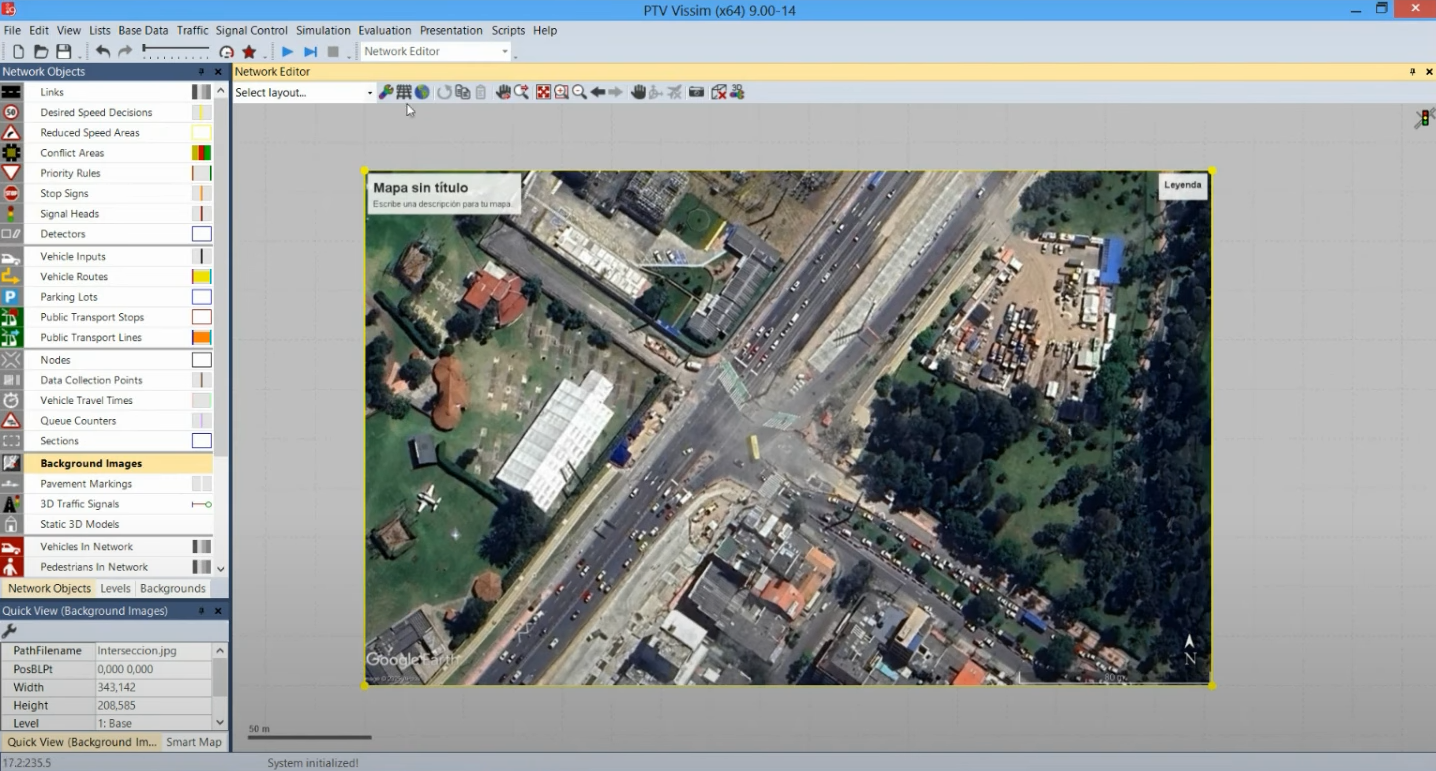
\includegraphics[width=0.92\linewidth,height=0.62\textheight,keepaspectratio]{./media/image127.png}
\captionof*{figure}{\small\itshape Figura 8. Sistema simulador de tráfico PTV VISSIM}
\addcontentsline{lof}{figure}{Figura 8. Sistema simulador de tráfico PTV VISSIM}
\label{fig:8}
\end{center}

\textbf{AIMSUN}

AIMSUN, desarrollado originalmente en la Universidad Politécnica de Cataluña y luego comercializado por TSS-Transport Simulation Systems, es un simulador híbrido micro-mesoscópico. Esto significa que puede operar tanto a nivel microscópico, similar a VISSIM, como a nivel mesoscópico, donde los vehículos se agrupan en flujos para acelerar el cálculo en redes grandes. AIMSUN se utiliza ampliamente en organismos de planificación y ofrece capacidades avanzadas de simulación de semáforos y lógica adaptativa. Permite cargar planes SCATS o SCOOT reales y replicar su comportamiento, o probar nuevos algoritmos mediante su API. Además, sus gráficos 2D/3D permiten construir una representación completa de la infraestructura urbana (semáforos, señales, paradas de bus, etc.) (Bedoya Reyes, 2013). AIMSUN ha incorporado en versiones recientes módulos para evaluar vehículos autónomos y conectados, y tiene una interfaz con herramientas de optimización en tiempo real, lo que lo posiciona como una plataforma adecuada para probar conceptos de ciudad inteligente. Aunque ambos simuladores, VISSIM y AIMSUN, pueden ofrecer resultados similares si están debidamente calibrados, AIMSUN suele requerir más experiencia en calibración, mientras que VISSIM es el preferido en algunos mercados por tradición. En la figura 19 podemos observar la interfaz del simulador AIMSUN.

\begin{center}
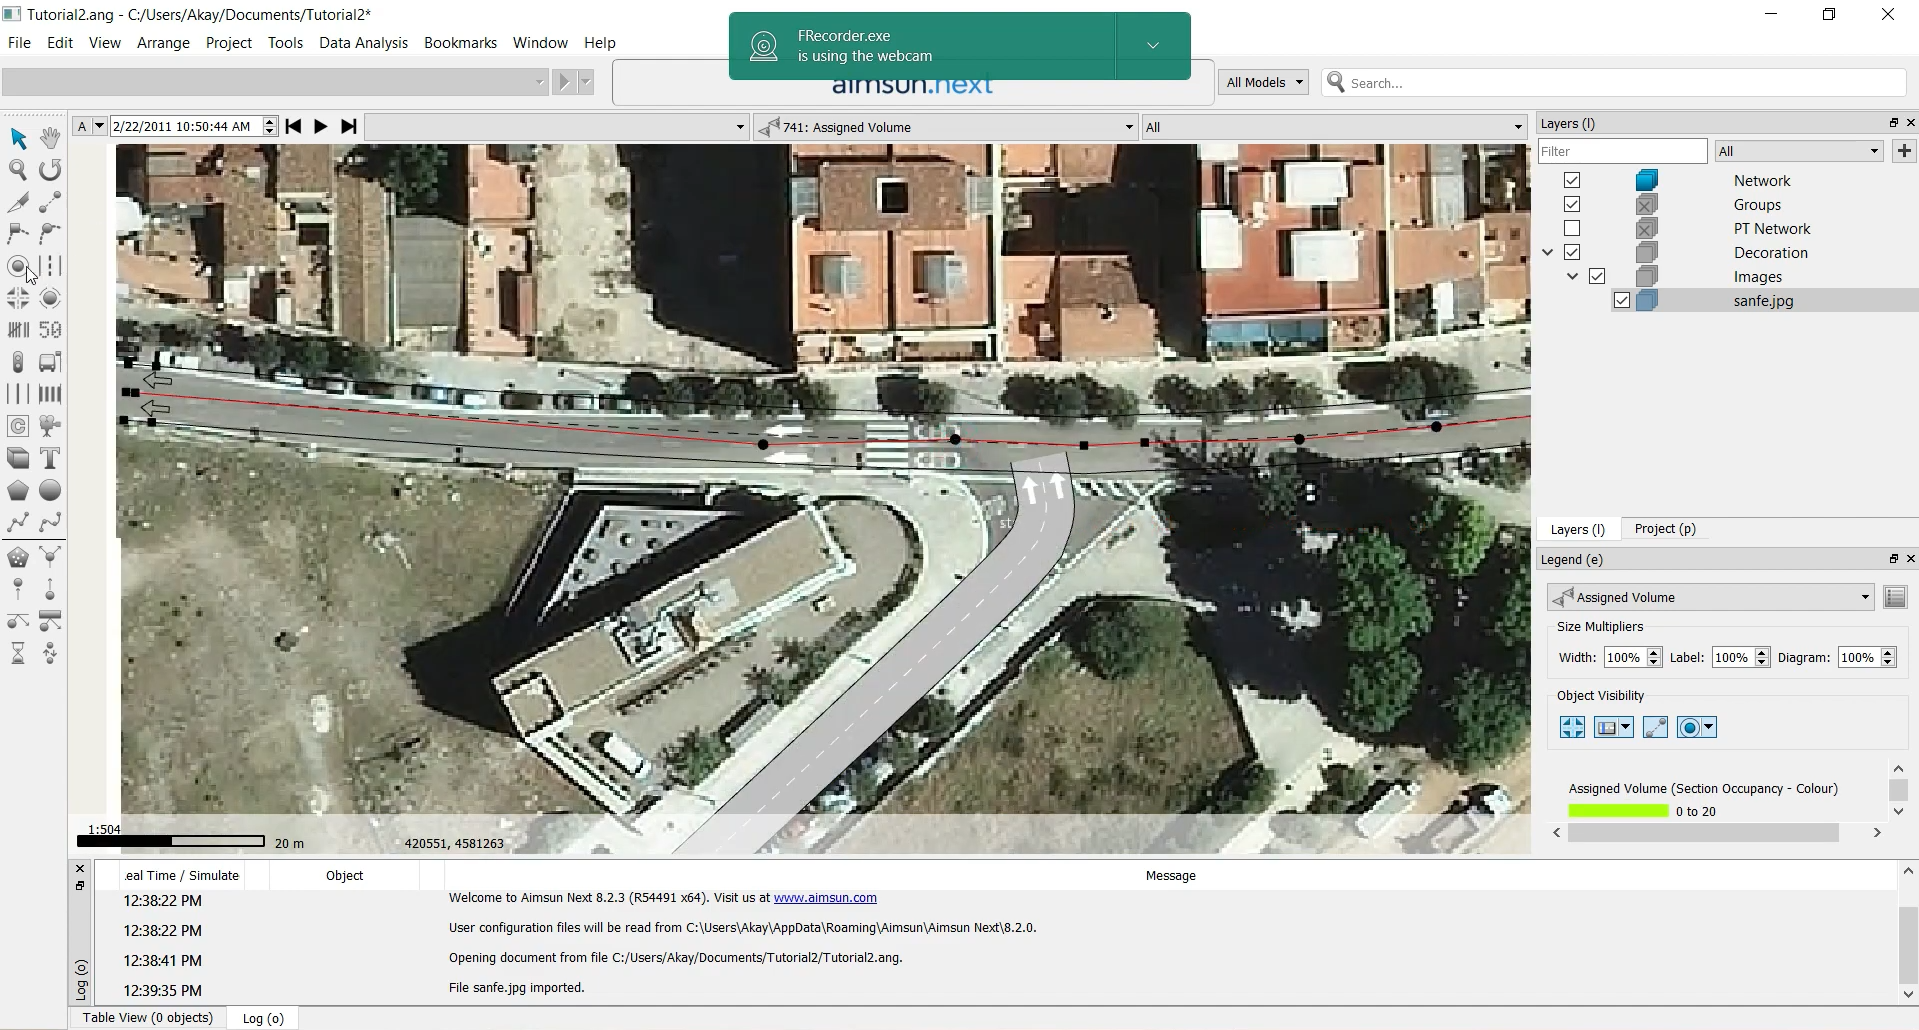
\includegraphics[width=0.92\linewidth,height=0.62\textheight,keepaspectratio]{./media/image132.png}
\captionof*{figure}{\small\itshape Figura 9. Simulador de control de tráfico híbrido micro-mesoscópico AIMSUN}
\addcontentsline{lof}{figure}{Figura 9. Simulador de control de tráfico híbrido micro-mesoscópico AIMSUN}
\label{fig:9}
\end{center}

\textbf{SUMO}

SUMO es un simulador de tráfico open-source (código abierto), mantenido por DLK (alemán) y una comunidad de usuarios, muy popular en el ámbito académico. Este simulador es microscópico por defecto y permite simular redes a gran escala con miles de intersecciones y vehículos. Su principal ventaja es ser gratuito y altamente personalizable/extensible. SUMO soporta características como semáforos, rutas de transporte público y peatones, y cuenta con el módulo TraCI (Traffic Control Interface), que permite la comunicación en vivo con la simulación. Esto permite que un programa externo (como un módulo de control IoT) se conecte a SUMO durante la ejecución y pueda consultar el estado del tráfico o imponer acciones como cambiar la luz de un semáforo, lo que lo hace ideal para probar algoritmos de control adaptativo en lazo cerrado. SUMO también soporta comunicaciones vehiculares simuladas e importación de mapas reales (OpenStreetMap). En términos de exactitud, al ser open-source, SUMO requiere calibración manual cuidadosa para reflejar condiciones reales, y su motor de simulación es algo más simplificado que el de VISSIM o AIMSUN en ciertos aspectos de dinámica vehicular. A pesar de esto, su desempeño computacional es muy bueno, pudiendo simular grandes redes más rápidamente que algunos competidores debido a su optimización y la posibilidad de simulación distribuida. En la figura 20 podemos observar la interfaz del simulador SUMO.

\begin{center}
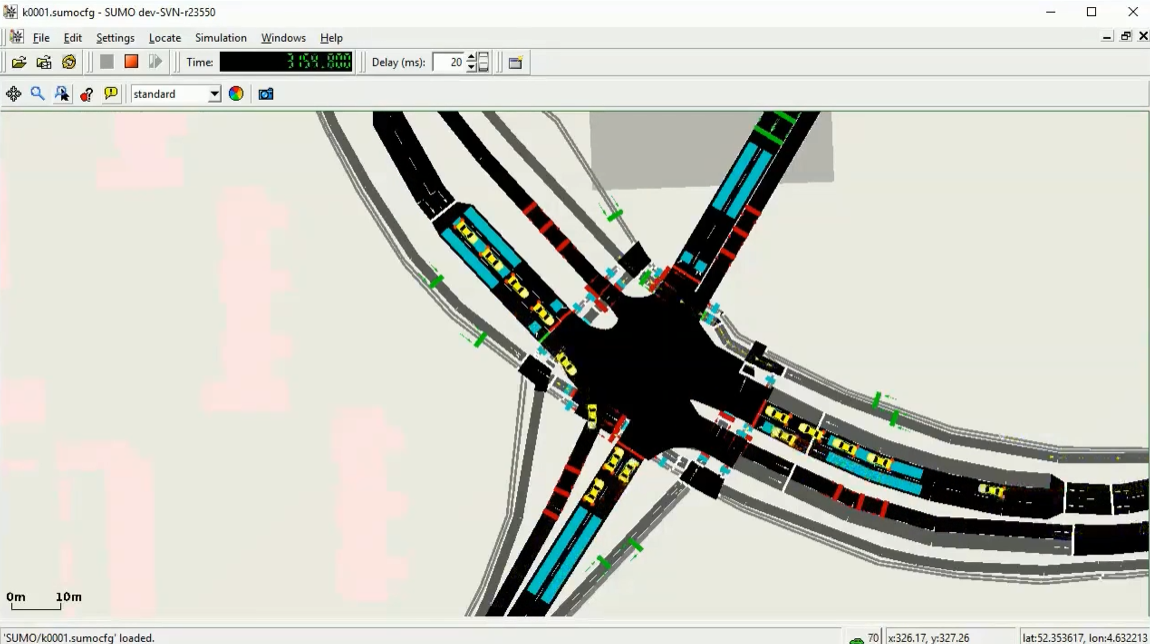
\includegraphics[width=0.92\linewidth,height=0.62\textheight,keepaspectratio]{./media/image144.png}
\captionof*{figure}{\small\itshape Figura 10. Sistema de control alemán de tráfico Open - Source SUMO}
\addcontentsline{lof}{figure}{Figura 10. Sistema de control alemán de tráfico Open - Source SUMO}
\label{fig:10}
\end{center}

\textbf{Synchro 8}\\
Synchro 8 es una herramienta de análisis y optimización de semáforos desarrollada por Trafficware (ahora parte de Cubic Corporation), diseñada para ofrecer capacidades de simulación y optimización del tráfico a nivel de intersecciones y redes viales. Esta versión ha mejorado significativamente en comparación con sus predecesoras, incorporando el motor computacional del \emph{Manual de Capacidad de Carreteras (HCM) 2010}, lo que proporciona un análisis más preciso de intersecciones semaforizadas y no semaforizadas. Además, Synchro 8 permite simulaciones en tiempo real mediante su integración con SimTraffic, lo que posibilita visualizar el comportamiento del tráfico en escenarios dinámicos. También es compatible con el formato \emph{Universal Traffic Data Format (UTDF)}, lo que facilita la integración con otros simuladores, como AIMSUN, para realizar co-simulaciones entre modelos microscópicos y mesoscópicos. La interfaz de usuario ha sido optimizada para mejorar la experiencia de configuración y visualización de los modelos, permitiendo importar mapas de fondo y ver los resultados en 3D. (Trafficware, 2014).\\
En la figura 19 podemos observar la interfaz de la herramienta de análisis Synchro 8.

\begin{center}
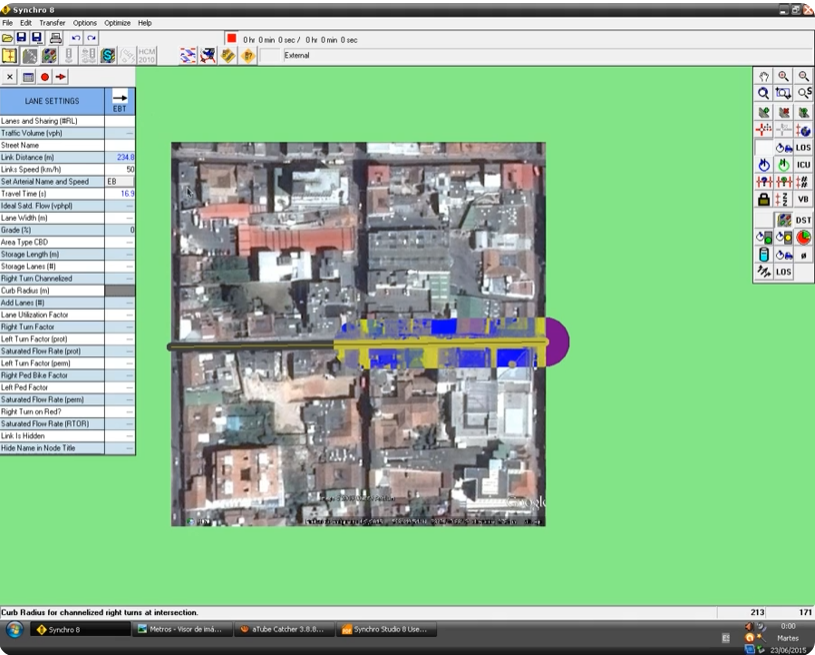
\includegraphics[width=0.92\linewidth,height=0.62\textheight,keepaspectratio]{./media/image45.png}
\captionof*{figure}{\small\itshape Figura 11. Synchro 8: análisis y optimización de semáforos}
\addcontentsline{lof}{figure}{Figura 11. Synchro 8: análisis y optimización de semáforos}
\label{fig:11}
\end{center}

\Needspace{6\baselineskip}
\captionof*{table}{\small\bfseries Tabla 2.6. Comparativa de simuladores de tráfico (Creación propia).}
\addcontentsline{lot}{table}{Tabla 2.6. Comparativa de simuladores de tráfico (Creación propia).}
\label{tbl:2.6}

\begin{longtable}[]{@{}
  >{\raggedright\arraybackslash}p{(\columnwidth - 8\tabcolsep) * \real{0.2000}}
  >{\raggedright\arraybackslash}p{(\columnwidth - 8\tabcolsep) * \real{0.2000}}
  >{\raggedright\arraybackslash}p{(\columnwidth - 8\tabcolsep) * \real{0.2000}}
  >{\raggedright\arraybackslash}p{(\columnwidth - 8\tabcolsep) * \real{0.2000}}
  >{\raggedright\arraybackslash}p{(\columnwidth - 8\tabcolsep) * \real{0.2000}}@{}}
\toprule
\begin{minipage}[b]{\linewidth}\raggedright
\textbf{Simulador}
\end{minipage} & \begin{minipage}[b]{\linewidth}\raggedright
\textbf{Tipo}
\end{minipage} & \begin{minipage}[b]{\linewidth}\raggedright
\textbf{Características Principales}
\end{minipage} & \begin{minipage}[b]{\linewidth}\raggedright
\textbf{Integración con Sistemas Externos}
\end{minipage} & \begin{minipage}[b]{\linewidth}\raggedright
\textbf{Comentarios}
\end{minipage} \\
\begin{minipage}[b]{\linewidth}\raggedright
PTV VISSIM
\end{minipage} & \begin{minipage}[b]{\linewidth}\raggedright
Microscópico
\end{minipage} & \begin{minipage}[b]{\linewidth}\raggedright
Control adaptativo, semáforos programables, comunicación V2X
\end{minipage} & \begin{minipage}[b]{\linewidth}\raggedright
APIs externas, módulos para IoT
\end{minipage} & \begin{minipage}[b]{\linewidth}\raggedright
Visualización en 3D. Es flexible y permite integrarse con lógicas de control personalizadas.
\end{minipage} \\
\begin{minipage}[b]{\linewidth}\raggedright
AIMSUN
\end{minipage} & \begin{minipage}[b]{\linewidth}\raggedright
Híbrido (micro-mesoscópico)
\end{minipage} & \begin{minipage}[b]{\linewidth}\raggedright
Planes SCATS/SCOOT, vehículos autónomos, optimización en tiempo real
\end{minipage} & \begin{minipage}[b]{\linewidth}\raggedright
API para algoritmos, herramientas de optimización
\end{minipage} & \begin{minipage}[b]{\linewidth}\raggedright
Permite la simulación avanzada de vehículos autónomos y se integra bien con herramientas de optimización.
\end{minipage} \\
\begin{minipage}[b]{\linewidth}\raggedright
SUMO
\end{minipage} & \begin{minipage}[b]{\linewidth}\raggedright
Microscópico (Open-source)
\end{minipage} & \begin{minipage}[b]{\linewidth}\raggedright
Módulo TraCI, comunicaciones vehiculares simuladas
\end{minipage} & \begin{minipage}[b]{\linewidth}\raggedright
Comunicación en vivo con la simulación
\end{minipage} & \begin{minipage}[b]{\linewidth}\raggedright
Gratuito y altamente personalizable Maneja Control adaptativo.
\end{minipage} \\
\begin{minipage}[b]{\linewidth}\raggedright
Synchro 8
\end{minipage} & \begin{minipage}[b]{\linewidth}\raggedright
Mesoscópico
\end{minipage} & \begin{minipage}[b]{\linewidth}\raggedright
Integración con VISSIM, optimización de flujo vehicular
\end{minipage} & \begin{minipage}[b]{\linewidth}\raggedright
Integración con otros simuladores
\end{minipage} & \begin{minipage}[b]{\linewidth}\raggedright
Una interfaz de usuario optimizada y capacidades de simulación en tiempo real.
\end{minipage} \\
\midrule
\endhead
\bottomrule
\endlastfoot
\end{longtable}

En el contexto de esta tesis, la simulación será útil para validar el módulo de control adaptativo IoT antes de considerarse su implementación física. La elección del simulador dependerá de criterios como la disponibilidad, la facilidad de conectar el algoritmo externo, y la necesidad de detalle. Dado que se busca probar comunicación con la nube y ciberseguridad, un simulador flexible como SUMO con TraCI permitiría simular ataques cibernéticos y evaluar la respuesta del sistema. Alternativamente, si se requiere un entorno más visual para mostrar resultados a stakeholders, podría usarse VISSIM o AIMSUN en alguna fase para demostrar la operación del algoritmo en una intersección modelo de la ciudad estudiada.

Se deduce que es factible emular con realismo las condiciones de tráfico y las interacción con nuestro módulo IoT antes de realizar una intersección real. La comparación de simuladores sugiere que adoptaremos SUMO para las pruebas iniciales de nuestro controlador adaptativo por su apertura y capacidad de integración en tiempo real, complementando con VISSIM/AIMSUN para validaciones puntuales de micro detalle o presentación visual.

\Needspace{6\baselineskip}
\captionof*{table}{\small\bfseries Tabla 2.7. Síntesis del estado del arte y criterios adoptados para la solución propuesta. (Creación propia).}
\addcontentsline{lot}{table}{Tabla 2.7. Síntesis del estado del arte y criterios adoptados para la solución propuesta. (Creación propia).}
\label{tbl:2.7}

\begin{longtable}[]{@{}
  >{\raggedright\arraybackslash}p{(\columnwidth - 6\tabcolsep) * \real{0.2100}}
  >{\raggedright\arraybackslash}p{(\columnwidth - 6\tabcolsep) * \real{0.3000}}
  >{\raggedright\arraybackslash}p{(\columnwidth - 6\tabcolsep) * \real{0.2400}}
  >{\raggedright\arraybackslash}p{(\columnwidth - 6\tabcolsep) * \real{0.2500}}@{}}
\toprule
\begin{minipage}[b]{\linewidth}\raggedright
\textbf{Eje tecnológico}
\end{minipage} & \begin{minipage}[b]{\linewidth}\raggedright
\textbf{Lección del estado del arte}
\end{minipage} & \begin{minipage}[b]{\linewidth}\raggedright
\textbf{Criterio adoptado}
\end{minipage} & \begin{minipage}[b]{\linewidth}\raggedright
\textbf{Aplicación en la tesis}
\end{minipage} \\
\begin{minipage}[b]{\linewidth}\raggedright
Sensado vehicular
\end{minipage} & \begin{minipage}[b]{\linewidth}\raggedright
La visión por computadora permite obtener flujo, colas y clasificación, aunque requiere calibración y respaldo ante condiciones adversas.
\end{minipage} & \begin{minipage}[b]{\linewidth}\raggedright
Usar cámara como fuente principal y sensores auxiliares para diagnóstico.
\end{minipage} & \begin{minipage}[b]{\linewidth}\raggedright
Módulo IoT con cámara, sensores ambientales y monitoreo energético.
\end{minipage} \\
\begin{minipage}[b]{\linewidth}\raggedright
Control adaptativo
\end{minipage} & \begin{minipage}[b]{\linewidth}\raggedright
Los sistemas híbridos combinan respuesta local rápida con coordinación global.
\end{minipage} & \begin{minipage}[b]{\linewidth}\raggedright
Priorizar control difuso local validable y dejar optimización global como capa de recomendación.
\end{minipage} & \begin{minipage}[b]{\linewidth}\raggedright
Control local autónomo, coordinación por nube y validación en simulación.
\end{minipage} \\
\begin{minipage}[b]{\linewidth}\raggedright
Comunicaciones
\end{minipage} & \begin{minipage}[b]{\linewidth}\raggedright
La interoperabilidad requiere separar protocolos industriales de telemetría IoT.
\end{minipage} & \begin{minipage}[b]{\linewidth}\raggedright
NTCIP para entorno semafórico y MQTT/TLS para telemetría.
\end{minipage} & \begin{minipage}[b]{\linewidth}\raggedright
Arquitectura compatible con controlador existente y servicios en Azure.
\end{minipage} \\
\begin{minipage}[b]{\linewidth}\raggedright
Ciberseguridad
\end{minipage} & \begin{minipage}[b]{\linewidth}\raggedright
Los sistemas conectados requieren autenticación, cifrado y trazabilidad.
\end{minipage} & \begin{minipage}[b]{\linewidth}\raggedright
Diseñar defensa por capas y modo degradado seguro.
\end{minipage} & \begin{minipage}[b]{\linewidth}\raggedright
TLS, MFA, RBAC, auditoría y conservación del controlador como autoridad final.
\end{minipage} \\
\begin{minipage}[b]{\linewidth}\raggedright
Validación
\end{minipage} & \begin{minipage}[b]{\linewidth}\raggedright
La simulación permite comparar estrategias antes de intervenir infraestructura vial real.
\end{minipage} & \begin{minipage}[b]{\linewidth}\raggedright
Usar SUMO/TraCI para escenarios reproducibles.
\end{minipage} & \begin{minipage}[b]{\linewidth}\raggedright
Evaluación de métricas de cola, espera, velocidad y congestión.
\end{minipage} \\
\midrule
\endhead
\bottomrule
\endlastfoot
\end{longtable}

\chapter{DISEÑO CONCEPTUAL}\label{capuxedtulo-3-diseuxf1o-conceptual}

En este capítulo, se detallan los requisitos que debe cumplir la propuesta de solución para un sistema de control adaptativo inteligente de la red semafórica vial en Lima. Se comienza con el análisis de los principales actores involucrados, sus necesidades y los requerimientos clave para el desarrollo del sistema. Luego, se presenta una representación del sistema como una ``caja negra'', identificando las entradas, salidas y los procesos necesarios para obtener las salidas requeridas. Además, se evalúan diversas alternativas de solución para los problemas planteados en la introducción de esta tesis, con una evaluación técnico-económica para determinar la viabilidad de cada alternativa. Finalmente, se presentará el concepto de solución óptima que se utilizará en la fase de desarrollo.

El propósito de este diseño conceptual es abordar las necesidades surgidas de la problemática del sistema semafórico actual en Lima, caracterizado por ineficiencia, descoordinación y falta de adaptabilidad al flujo vehicular. Para ello, se identifican los actores clave y sus necesidades, seguidas de los requerimientos esenciales para garantizar la efectividad del sistema propuesto.

A continuación, se detallan los principales actores involucrados y sus respectivas necesidades, basados en entrevistas con expertos y encuestas realizadas a los usuarios del sistema actual.

\section{Actores clave y necesidades}\label{actores-clave-y-necesidades}

En el caso del diseño conceptual para la red semafórica adaptativa, los actores clave incluyen al cliente principal (la Municipalidad de Lima), los usuarios directos (conductores y peatones), los usuarios indirectos (operativos de tráfico y administradores de la infraestructura), así como los interesados secundarios como las autoridades de seguridad vial. Cada uno de estos actores tiene necesidades específicas que deben ser atendidas para asegurar la efectividad y eficiencia del sistema propuesto. A continuación, se describen las necesidades de cada grupo, basadas en entrevistas con expertos y encuestas realizadas a los usuarios del sistema actual.

\textbf{Cliente (Municipalidad de Lima / Subgerencia de Gestión de Movilidad Urbana):}

Mejorar la coordinación y eficiencia de la red semafórica en tiempo real, optimizando la gestión del tráfico mediante un sistema adaptativo que ajuste dinámicamente los ciclos semafóricos según el flujo vehicular. La infraestructura actual presenta una falta de sincronización, lo que provoca congestión y pérdidas económicas por tiempos de espera elevados.

Sistema de monitoreo en tiempo real, que permita la toma de decisiones basada en datos actualizados sobre el tráfico, facilitando la supervisión y el control remoto. Este monitoreo debe ser fácil de interpretar y brindar alertas sobre incidencias y desviaciones en el flujo de tráfico.

\textbf{Usuarios Finales (Conductores y Peatones):}

Reducir los tiempos de espera en las intersecciones semaforizadas para mejorar la fluidez del tráfico, especialmente en intersecciones con bajo flujo vehicular, como lo mencionaron los encuestados en las entrevistas realizadas, que reportaron largos tiempos de espera debido a semáforos mal coordinados.

Mejorar la seguridad vial, reduciendo accidentes causados por semáforos descoordinados y la frustración de los conductores por tiempos de espera excesivos. El sistema debe reducir la frustración de los conductores, lo que disminuye las conductas temerarias y mejora la experiencia general de los usuarios.

Los encuestados expresaron en la encuesta su \textbf{preocupación por la seguridad vial}, señalando que los tiempos de espera largos y la falta de coordinación entre los semáforos incrementan la probabilidad de \textbf{accidentes y conductas peligrosas}, como cambios de luces no respetados.

\textbf{Usuarios Indirectos (Operativos de Tráfico y Administradores de Infraestructura):}

Implementación de un sistema de comunicación centralizada, que permita la supervisión efectiva de la red semafórica, garantizando que las intersecciones estén sincronizadas y que se puedan tomar acciones correctivas eficientemente. Las entrevistas con operativos de tránsito confirmaron la necesidad de un sistema de monitoreo centralizado y fácil de gestionar para controlar las intersecciones desde un punto central.

Medidas de ciberseguridad: La infraestructura de los semáforos debe ser protegida contra posibles ataques cibernéticos, asegurando la integridad y confidencialidad de los datos del sistema. Según las entrevistas, la ciberseguridad es una preocupación clave, dado que el sistema debe operar de manera segura sin comprometer la privacidad de los datos de los usuarios ni ser vulnerable a manipulaciones externas.

\textbf{Usuarios Directos y Operativos (Conductores y Autoridades de Tránsito):}

Interfaz gráfica intuitiva: La implementación de una interfaz gráfica amigable es esencial para permitir el monitoreo en tiempo real y el ajuste ágil y preciso de los semáforos. Esta interfaz debe incluir alertas automáticas sobre desviaciones en el flujo de tráfico, como mencionaron los encuestados, quienes también destacaron la necesidad de alertas visuales que ayuden a los operativos a tomar decisiones rápidamente en situaciones imprevistas.\\
\strut \\
Datos en tiempo real: La capacidad de recibir información en tiempo real sobre el estado de los semáforos es una prioridad tanto para conductores como para las autoridades. Esto permitiría una respuesta rápida ante emergencias o cambios en el flujo vehicular.

\textbf{Resultados de la Encuesta a Usuarios Finales:}

Las respuestas obtenidas en la encuesta respaldan las necesidades mencionadas. \textbf{El 60\% de los encuestados consideraron que la reducción de los tiempos de espera es muy importante}. La \textbf{sincronización entre semáforos} fue destacada por \textbf{el 40\%} de los encuestados como un aspecto clave para mejorar la experiencia en las intersecciones. Otro punto relevante fue la \textbf{seguridad vial}, donde \textbf{el 50\%} de las respuestas indicaron que las conductas peligrosas de los conductores, debido a la frustración causada por el sistema semafórico actual, son uno de los principales problemas.

\section{Lista de requerimientos}\label{lista-de-requerimientos}

Los requerimientos del sistema se identificaron a partir del análisis de las necesidades de los usuarios y las especificaciones técnicas necesarias para cumplir con los objetivos establecidos. Algunos de estos son obligatorios para garantizar un funcionamiento óptimo, mientras que otros representan deseos adicionales que mejoran el diseño final. Los criterios se detallan a continuación en la Tabla 3.1.

\Needspace{6\baselineskip}
\captionof*{table}{\small\bfseries Tabla 3.1. Lista de Requerimientos. (Creación propia)}
\addcontentsline{lot}{table}{Tabla 3.1. Lista de Requerimientos. (Creación propia)}
\label{tbl:3.1}

\begin{longtable}[]{@{}
  >{\raggedright\arraybackslash}p{(\columnwidth - 6\tabcolsep) * \real{0.1820}}
  >{\raggedright\arraybackslash}p{(\columnwidth - 6\tabcolsep) * \real{0.1311}}
  >{\raggedright\arraybackslash}p{(\columnwidth - 6\tabcolsep) * \real{0.5230}}
  >{\raggedright\arraybackslash}p{(\columnwidth - 6\tabcolsep) * \real{0.1639}}@{}}
\toprule
\multicolumn{3}{@{}>{\raggedright\arraybackslash}p{(\columnwidth - 6\tabcolsep) * \real{0.8361} + 4\tabcolsep}}{%
\multirow{2}{=}{\begin{minipage}[b]{\linewidth}\raggedright
LISTA DE REQUERIMIENTOS
\end{minipage}}} & \begin{minipage}[b]{\linewidth}\raggedright
Pág. 1 de 1
\end{minipage} \\
& & & \begin{minipage}[b]{\linewidth}\raggedright
Edición:1
\end{minipage} \\
\multicolumn{2}{@{}>{\raggedright\arraybackslash}p{(\columnwidth - 6\tabcolsep) * \real{0.3131} + 2\tabcolsep}}{%
\multirow{2}{=}{\begin{minipage}[b]{\linewidth}\raggedright
PROYECTO:
\end{minipage}}} & \multirow{2}{=}{\begin{minipage}[b]{\linewidth}\raggedright
DISEÑO DE UN SISTEMA DE CONTROL ADAPTATIVO INTELIGENTE DE LA RED SEMAFÓRICA VIAL QUE INCLUYE COMUNICACIÓN CON LA NUBE Y SEGURIDAD CIBERNÉTICA
\end{minipage}} & \multirow{2}{=}{\begin{minipage}[b]{\linewidth}\raggedright
Fecha: 21/04/25
\end{minipage}} \\
 \\
\multicolumn{2}{@{}>{\raggedright\arraybackslash}p{(\columnwidth - 6\tabcolsep) * \real{0.3131} + 2\tabcolsep}}{%
\begin{minipage}[b]{\linewidth}\raggedright
CLIENTE:
\end{minipage}} & \begin{minipage}[b]{\linewidth}\raggedright
Municipalidad Metropolitana de Lima
\end{minipage} & \begin{minipage}[b]{\linewidth}\raggedright
Elaborado:
\end{minipage} \\
\begin{minipage}[b]{\linewidth}\raggedright
Tipo
\end{minipage} & \begin{minipage}[b]{\linewidth}\raggedright
Deseo o Exigencia
\end{minipage} & \begin{minipage}[b]{\linewidth}\raggedright
DESCRIPCIÓN
\end{minipage} & \begin{minipage}[b]{\linewidth}\raggedright
Tumbalobos
\end{minipage} \\
\begin{minipage}[b]{\linewidth}\raggedright
Función Principal
\end{minipage} & \begin{minipage}[b]{\linewidth}\raggedright
Exigencia
\end{minipage} & \multicolumn{2}{>{\raggedright\arraybackslash}p{(\columnwidth - 6\tabcolsep) * \real{0.6869} + 2\tabcolsep}@{}}{%
\begin{minipage}[b]{\linewidth}\raggedright
Sistema inteligente de semaforización adaptativa que optimiza la gestión del tráfico en tiempo real utilizando sensores IoT para la recolección de datos de tráfico, comunicación en la nube y algoritmos de inteligencia artificial.
\end{minipage}} \\
\begin{minipage}[b]{\linewidth}\raggedright
Energía
\end{minipage} & \begin{minipage}[b]{\linewidth}\raggedright
Exigencia
\end{minipage} & \multicolumn{2}{>{\raggedright\arraybackslash}p{(\columnwidth - 6\tabcolsep) * \real{0.6869} + 2\tabcolsep}@{}}{%
\begin{minipage}[b]{\linewidth}\raggedright
El sistema de alimentación del módulo IoT debe contar con alimentación de respaldo capaz de operar durante un mínimo de 1 hora en caso de corte de energía principal, garantizando la continuidad del funcionamiento del semáforo inteligente. La fuente de energía será continua (DC), con un voltaje de 12V o 24V según los requisitos específicos del sistema. Además, el sistema deberá contar con una conexión a la red eléctrica para su alimentación principal, asegurando que el módulo IoT se recargue y mantenga operativo bajo condiciones normales.
\end{minipage}} \\
\begin{minipage}[b]{\linewidth}\raggedright
Fuerzas
\end{minipage} & \begin{minipage}[b]{\linewidth}\raggedright
Exigencia
\end{minipage} & \multicolumn{2}{>{\raggedright\arraybackslash}p{(\columnwidth - 6\tabcolsep) * \real{0.6869} + 2\tabcolsep}@{}}{%
\begin{minipage}[b]{\linewidth}\raggedright
El módulo debe soportar el peso de sus componentes internos, como la placa, el microcontrolador, los sensores y los actuadores así como de su propia estructura.
\end{minipage}} \\
\begin{minipage}[b]{\linewidth}\raggedright
Materia
\end{minipage} & \begin{minipage}[b]{\linewidth}\raggedright
Exigencia
\end{minipage} & \multicolumn{2}{>{\raggedright\arraybackslash}p{(\columnwidth - 6\tabcolsep) * \real{0.6869} + 2\tabcolsep}@{}}{%
\begin{minipage}[b]{\linewidth}\raggedright
El módulo IoT debe ser resistente a condiciones extremas como altas temperaturas, humedad, polvo y exposición al sol. Debe ser impermeable, resistente al vandalismo, y tener una carcasa robusta para soportar golpes y caídas. Los componentes internos deben estar aislados y protegidos contra cortocircuitos y daños físicos.
\end{minipage}} \\
\begin{minipage}[b]{\linewidth}\raggedright
Comunicación
\end{minipage} & \begin{minipage}[b]{\linewidth}\raggedright
Exigencia
\end{minipage} & \multicolumn{2}{>{\raggedright\arraybackslash}p{(\columnwidth - 6\tabcolsep) * \real{0.6869} + 2\tabcolsep}@{}}{%
\begin{minipage}[b]{\linewidth}\raggedright
Implementación del sistema de comunicación NTCIP entre semáforos y la plataforma de control centralizada, con conexión a una base de datos para el registro y análisis de las inspecciones.
\end{minipage}} \\
\begin{minipage}[b]{\linewidth}\raggedright
Control
\end{minipage} & \begin{minipage}[b]{\linewidth}\raggedright
Exigencia
\end{minipage} & \multicolumn{2}{>{\raggedright\arraybackslash}p{(\columnwidth - 6\tabcolsep) * \real{0.6869} + 2\tabcolsep}@{}}{%
\begin{minipage}[b]{\linewidth}\raggedright
Sistema de control adaptativo que ajuste los ciclos semafóricos según las condiciones del tráfico en tiempo real, con infraestructura escalable para integrar futuras intersecciones. Además, el sistema debe integrar algoritmos de aprendizaje automático para mejorar la predicción de flujo vehicular a medida que se recopilan más datos.
\end{minipage}} \\
\begin{minipage}[b]{\linewidth}\raggedright
Software
\end{minipage} & \begin{minipage}[b]{\linewidth}\raggedright
Exigencia
\end{minipage} & \multicolumn{2}{>{\raggedright\arraybackslash}p{(\columnwidth - 6\tabcolsep) * \real{0.6869} + 2\tabcolsep}@{}}{%
\begin{minipage}[b]{\linewidth}\raggedright
El software que controle el módulo IoT debe ser capaz de gestionar los algoritmos de control adaptativo del semáforo, procesar los datos de los sensores en tiempo real, y optimizar los ciclos semafóricos basados en las condiciones del tráfico. Este software debe garantizar una actualización remota a través de la nube. Además, debe contar con protocolos de seguridad cibernética robustos, siguiendo los estándares internacionales para garantizar la integridad de los datos.
\end{minipage}} \\
\begin{minipage}[b]{\linewidth}\raggedright
Uso
\end{minipage} & \begin{minipage}[b]{\linewidth}\raggedright
Exigencia
\end{minipage} & \multicolumn{2}{>{\raggedright\arraybackslash}p{(\columnwidth - 6\tabcolsep) * \real{0.6869} + 2\tabcolsep}@{}}{%
\begin{minipage}[b]{\linewidth}\raggedright
Sistema que garantice la interoperabilidad con los semáforos existentes en Lima (compatibilidad con controladores actuales).
\end{minipage}} \\
\begin{minipage}[b]{\linewidth}\raggedright
Seguridad
\end{minipage} & \begin{minipage}[b]{\linewidth}\raggedright
Exigencia
\end{minipage} & \multicolumn{2}{>{\raggedright\arraybackslash}p{(\columnwidth - 6\tabcolsep) * \real{0.6869} + 2\tabcolsep}@{}}{%
\begin{minipage}[b]{\linewidth}\raggedright
Seguridad cibernética de acuerdo con los estándares internacionales (IEC 62443), protegiendo la infraestructura contra posibles ataques.

Diseño del módulo de IoT resistente a condiciones climáticas extremas y vandalismo (P65).
\end{minipage}} \\
\begin{minipage}[b]{\linewidth}\raggedright
Geometría
\end{minipage} & \begin{minipage}[b]{\linewidth}\raggedright
Deseo
\end{minipage} & \multicolumn{2}{>{\raggedright\arraybackslash}p{(\columnwidth - 6\tabcolsep) * \real{0.6869} + 2\tabcolsep}@{}}{%
\begin{minipage}[b]{\linewidth}\raggedright
Módulo IoT de un tamaño máximo de 70x70x80 cm
\end{minipage}} \\
\begin{minipage}[b]{\linewidth}\raggedright
Precio
\end{minipage} & \begin{minipage}[b]{\linewidth}\raggedright
Deseo
\end{minipage} & \multicolumn{2}{>{\raggedright\arraybackslash}p{(\columnwidth - 6\tabcolsep) * \real{0.6869} + 2\tabcolsep}@{}}{%
\begin{minipage}[b]{\linewidth}\raggedright
La solución debe ser de bajo costo, con un presupuesto máximo estimado de 10000 soles por intersección.
\end{minipage}} \\
\midrule
\endhead
\bottomrule
\endlastfoot
\end{longtable}

\section{Estructura de funciones}\label{estructura-de-funciones}

En este apartado se presenta el modelo de caja negra del sistema, junto con la lista y estructura de sus funciones.

\subsection{Black box}\label{black-box}

En la Figura 22 se presenta la caja negra del sistema de control adaptativo inteligente de la red semafórica. Se describen las entradas y salidas según el siguiente formato:

\begin{itemize}
\item
  Las líneas punteadas representan señales
\item
  Las líneas delgadas representan la energía
\item
  Las líneas gruesas representan la materia
\end{itemize}

\begin{center}
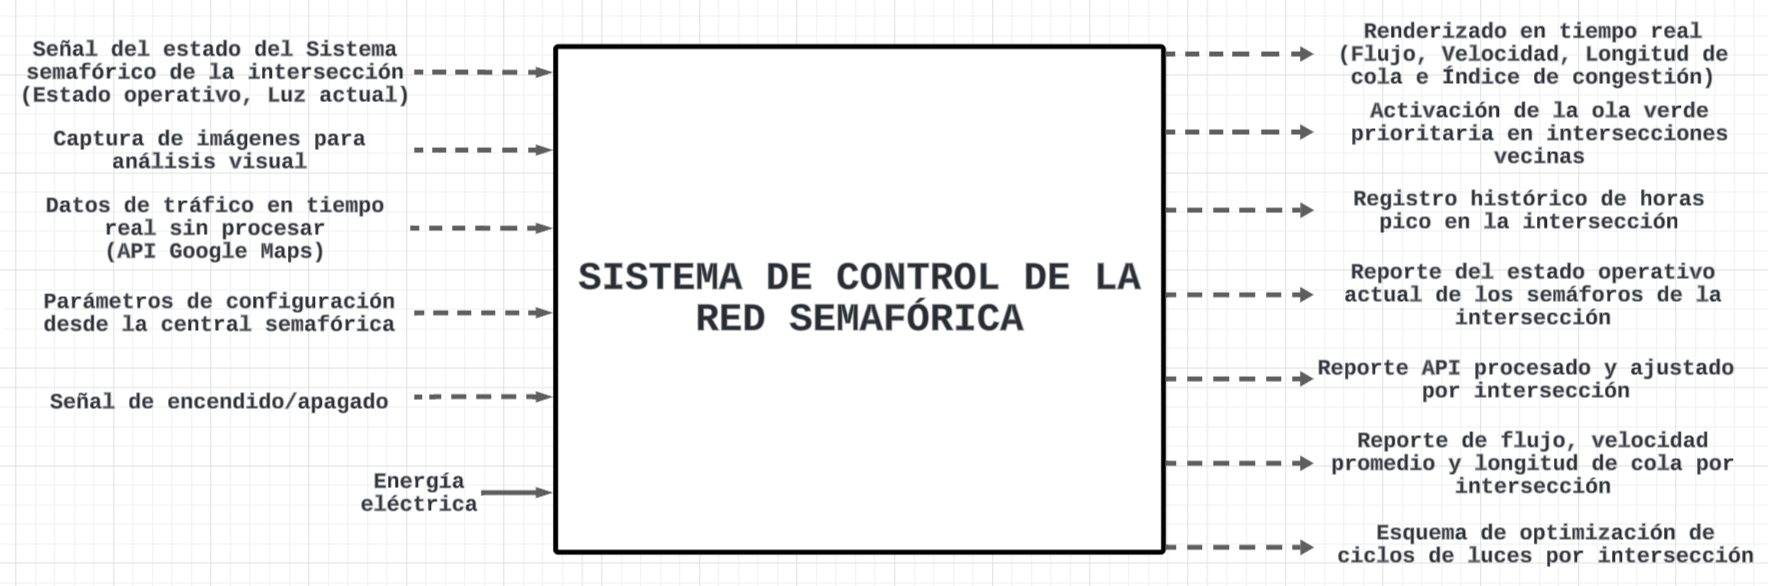
\includegraphics[width=0.92\linewidth,height=0.62\textheight,keepaspectratio]{./media/image91.png}
\captionof*{figure}{\small\itshape Figura 12. Caja negra del sistema (Creación propia).}
\addcontentsline{lof}{figure}{Figura 12. Caja negra del sistema (Creación propia).}
\label{fig:12}
\end{center}

SEÑALES DE ENTRADA:

\textbf{Señal del estado del Sistema semafórico de la intersección (Estado operativo, Luz actual):}

\begin{quote}
Esta señal entrega una lista de datos crudos del estado actual del sistema, estos datos se reciben para procesamiento interno y fusión con otros datos relevantes del sistema. Su utilidad recae en que nos permite monitorear la operatividad de cada semáforo de la intersección.
\end{quote}

\textbf{Captura de imágenes para análisis visual:}

\begin{quote}
Habrá una captura de imágenes en tiempo real, provenientes de cámaras que se instalarán en el sistema, esta señal de vídeo de las cámaras se utiliza en el sistema para identificar vehículos de emergencia (como ambulancias o bomberos). Esta entrada permite darles prioridad en el tráfico, cambiando el semáforo a favor de estos vehículos para permitirles pasar con las mínimas interrupciones, optimizando su tiempo de llegada a su destino. También será utilizada para detectar el flujo general de vehículos, velocidad promedio y longitud de cola de espera.
\end{quote}

\textbf{Datos de tráfico en tiempo real sin procesar  (API Google Maps):}

A través de la API de Google Maps, el sistema extrae datos en tiempo real sobre las condiciones del tráfico en las calles cercanas y en la intersección donde se encuentre el semáforo en cuestión. Esto incluye la congestión actual y la velocidad promedio de los vehículos. Estos datos se utilizan para ajustar los ciclos de los semáforos y optimizar el flujo vehicular según las condiciones actuales, aumentando así la robustez al no solo depender de sensores físicos de los semáforos sino también con datos de fuentes digitales.

\textbf{Parámetros de configuración desde la central semafórica}

Señal proveniente de la central semafórica destinada a modificar los ciclos de la intersección.

\textbf{Señal de encendido/apagado:}

Esta entrada indica si el sistema instalado está encendido o apagado.

\textbf{Energía eléctrica:}

Proporciona la potencia necesaria para operar todos los componentes eléctricos del sistema.

SEÑALES DE SALIDA:

\textbf{Esquema de optimización de ciclos de luces por intersección:}

La central semafórica recibe los resultados de optimización que proporciona el control adaptativo de la nube basadas en el análisis de los datos de tráfico y condiciones viales. Estos resultados son interpretados como sugerencias para el operario de la central semafórica quien las revisa y toma las decisiones pertinentes sobre cómo implementar las modificaciones en los ciclos de luces, considerando las condiciones actuales, las pautas establecidas en el sistema y su propia experiencia.

\textbf{Reporte del estado operativo actual de los semáforos de la intersección:}

\begin{quote}
Este reporte entrega una lista de datos del estado actual del sistema, como si está activo o inactivo, si presenta fallas, el tiempo de cada ciclo semafórico, la luz actualmente encendida. Su utilidad recae en que nos permite monitorear todo el sistema, enviando a la central semafórica una señal de necesidad de mantenimiento predictivo.
\end{quote}

\textbf{Registro histórico de horas pico en la intersección:}

\begin{quote}
En función a los datos del día se calculan las horas pico de esas intersecciones que se controlan por el controlador, esto es de utilidad pues nos permite predecir las horas pico de los próximos días permitiéndole al sistema generar una respuesta adecuada ajustada al flujo típico por días de la semana de la intersección donde se ha instalado.
\end{quote}

\textbf{Reporte API procesado y ajustado por intersección:}

\begin{quote}
Esta salida corresponde al resultado del procesamiento interno de los datos obtenidos de la API de tráfico (Google Maps) que han sido filtrados, corregidos y ajustados específicamente para la intersección en cuestión.
\end{quote}

\textbf{Reporte de flujo, velocidad promedio y longitud de cola por intersección:}

\begin{quote}
Este reporte entrega métricas calculadas en tiempo real sobre el tráfico en cada intersección. El flujo vehicular se refiere a la cantidad de vehículos que pasan por la intersección en un intervalo de tiempo determinado; la velocidad promedio indica la rapidez con la que se desplazan los vehículos, y la longitud de cola representa la cantidad de vehículos detenidos o esperando en la intersección.
\end{quote}

\textbf{Activación de la ola verde prioritaria en intersecciones vecinas:}

\begin{quote}
Esta señal se genera para coordinar la propagación de una ``ola verde'' entre intersecciones próximas, permitiendo que vehículos prioritarios, como ambulancias o bomberos, puedan avanzar de manera continua y sin interrupciones. El sistema activa esta función automáticamente cuando detecta vehículos de emergencia, predice la siguiente dirección del vehículo para realizar la ola verde en las intersección por donde pase, con el fin de disminuir su tiempo de llegada.
\end{quote}

\textbf{Renderizado en tiempo real (Flujo, Velocidad promedio, Longitud de cola e Índice de congestión):}

\begin{quote}
Salida visual que muestra en interfaces de monitoreo los parámetros clave del tráfico en la intersección, actualizados constantemente en tiempo real. Incluye el flujo vehicular, la velocidad promedio, la longitud de cola y un índice de congestión calculado que sintetiza el nivel de saturación del tráfico.
\end{quote}

\subsubsection{\texorpdfstring{3.3.2 Lista de funciones\\
}{3.3.2 Lista de funciones }}\label{lista-de-funciones}

El Sistema de Control Adaptativo Inteligente de la Red Semafórica Vial de Lima se basa en un sistema IoT que utiliza sensores y algoritmos de inteligencia artificial para optimizar la gestión del tráfico en tiempo real. El objetivo de este sistema es mejorar la fluidez del tránsito, reducir la congestión vehicular y, secundariamente, disminuir las emisiones contaminantes. A continuación se detallan a grandes rasgos las actividades relacionadas con preparación, ejecución, control y fase final del sistema.\\
\strut \\
\textbf{Preparación}

\begin{quote}
\textbf{Instalación del controlador y la cámara en su carcasa:}
\end{quote}

\begin{itemize}
\item
  Colocar la cámara con todos los mecanismos de seguridad en la carcasa del controlador.
\item
  Montar el controlador y conectar la circuitería involucrada (sensores, actuadores y comunicación).
\item
  Asegurar la correcta conexión de los semáforos a la red IoT para permitir la transmisión de datos en tiempo real.
\end{itemize}

\begin{quote}
\textbf{Conexión a la Nube:}
\end{quote}

\begin{itemize}
\item
  Asegurar la conectividad estable y segura de cada controlador con la nube para el envío y análisis de datos en la central semafórica.
\item
  Verificar la seguridad cibernética de las conexiones, implementando mecanismos de cifrado y autenticación.
\end{itemize}

\begin{quote}
\textbf{Prueba de Comunicación de Datos:}
\end{quote}

\begin{itemize}
\item
  Realizar pruebas para asegurar que la captura de imágenes, datos de sensores y API externas se reciban y procesen correctamente.
\end{itemize}

\textbf{Ejecución}

\begin{quote}
\textbf{Detección de Tráfico:}
\end{quote}

\begin{itemize}
\item
  Captura en tiempo real del flujo vehicular, velocidad promedio y longitud de cola mediante cámaras y sensores.
\item
  Incorporación de datos externos de tráfico (API Google Maps) ajustados y procesados para mayor robustez del sistema.
\item
  Aplicación de algoritmos de inteligencia artificial para análisis y predicción de congestión y demanda.
\end{itemize}

\textbf{Ajuste de los Ciclos Semafóricos:}

\begin{itemize}
\item
  Optimización de los tiempos de verde, ámbar y rojo según la demanda vehicular y las condiciones detectadas.
\item
  Coordinación con intersecciones vecinas para sincronización eficiente de ciclos y activación de ``ola verde''.
\end{itemize}

\begin{quote}
\textbf{Priorización de Vehículos de Emergencia:}
\end{quote}

\begin{itemize}
\item
  Identificación y seguimiento de vehículos prioritarios para generar rutas de paso con prioridad mediante activación de ola verde prioritaria en intersecciones involucradas.
\end{itemize}

\textbf{Control}

\begin{quote}
\textbf{Monitoreo de Datos en Tiempo Real:}
\end{quote}

\begin{itemize}
\item
  Supervisión constante del estado operativo de los semáforos, sensores y la calidad de datos recibidos.
\item
  Detección de anomalías, fallas o inconsistencias y emisión de alertas para mantenimiento o intervención inmediata.
\end{itemize}

\begin{quote}
\textbf{Mantenimiento Predictivo y Preventivo:}
\end{quote}

\begin{itemize}
\item
  Análisis continuo de parámetros operativos para anticipar posibles fallos o degradación de equipos y programar mantenimientos oportunos.
\end{itemize}

\begin{quote}
\textbf{Actualización de Parámetros de Control:}
\end{quote}

\begin{itemize}
\item
  Los algoritmos de control adaptativo actualizan continuamente los parámetros de los semáforos para adaptarse a los cambios en el flujo vehicular y las condiciones del tráfico.
\end{itemize}

\textbf{Fase Final}

\begin{quote}
\textbf{Recuperación y Almacenamiento de Datos:}

Registro histórico detallado de horas pico, flujos, velocidades, longitudes de cola y estados operativos almacenados en bases de datos centrales para análisis posterior.

\textbf{Generación de Informes:}
\end{quote}

\begin{itemize}
\item
  Estado operativo actual y tendencias históricas.
\item
  Rendimiento del sistema, tiempos de espera y eficiencia en la reducción de congestión.
\item
  Reportes de flujo vehicular, velocidad promedio, longitud de cola e índice de congestión.
\item
  Alertas y recomendaciones para mantenimiento y optimización futura.
\end{itemize}

\begin{quote}
\textbf{Visualización y renderizado en tiempo real:}
\end{quote}

\begin{itemize}
\item
  Interfaces gráficas para operadores con datos actualizados en tiempo real sobre el flujo, velocidad, cola e índice de congestión para la toma de decisiones.
\end{itemize}

\begin{quote}
\textbf{Operación continua o desactivación controlada:}
\end{quote}

\begin{itemize}
\item
  El sistema está diseñado para funcionar de manera continua, pero contempla modos de desactivación o reinicio controlados para mantenimiento, actualizaciones o reconfiguraciones.
\end{itemize}

\textbf{Gestión de Riesgos}

\textbf{Fallos en Sensores:\\
Riesgo:} Sensores defectuosos o mal calibrados.\\
\textbf{Mitigación:} Realizar pruebas periódicas de calibración y reportarlo desde la interfaz

\textbf{Conectividad en la nube:\\
Riesgo:} Interrupción en la comunicación entre la central semafórica y la nube.\\
\textbf{Mitigación:} Implementar un sistema de almacenamiento local de datos en caso de pérdida de conexión y restablecer la comunicación en cuanto sea posible (Sistema de reintento de conexión).

\textbf{Errores en el Algoritmo de Optimización:\\
Riesgo:} Los algoritmos de IA no responden correctamente a cambios inesperados en el tráfico.\\
\textbf{Mitigación:} Entrenar el modelo con una gran variedad de datos y realizar pruebas de validación en condiciones diferentes, maximizando la robustez. Se podría instalar, en caso fuese necesario un sistema adicional en cada controlador que sirva como controlador base en caso no haya comunicación con la nube o se detecte que las predicciones de la IA no tienen un accuracy relevante para el sistema.

\textbf{Vulnerabilidades de Ciberseguridad:\\
Riesgo:} Ataques cibernéticos que puedan comprometer el funcionamiento del sistema semafórico.\\
\textbf{Mitigación:} Realizar la comunicación de los datos desde la central semafórica y la nube, no directamente desde los semáforos e implementar técnicas de cifrado y seguridad ante ciberataques.

A continuación, en la figura 23 se presenta la estructura de funciones separada por los siguientes dominios:

\begin{itemize}
\item
  Dominio de interfaz
\item
  Dominio de Energía
\item
  Dominio de actuadores
\item
  Dominio de sensores
\item
  Dominio de control
\item
  Dominio mecánico
\end{itemize}

\begin{center}
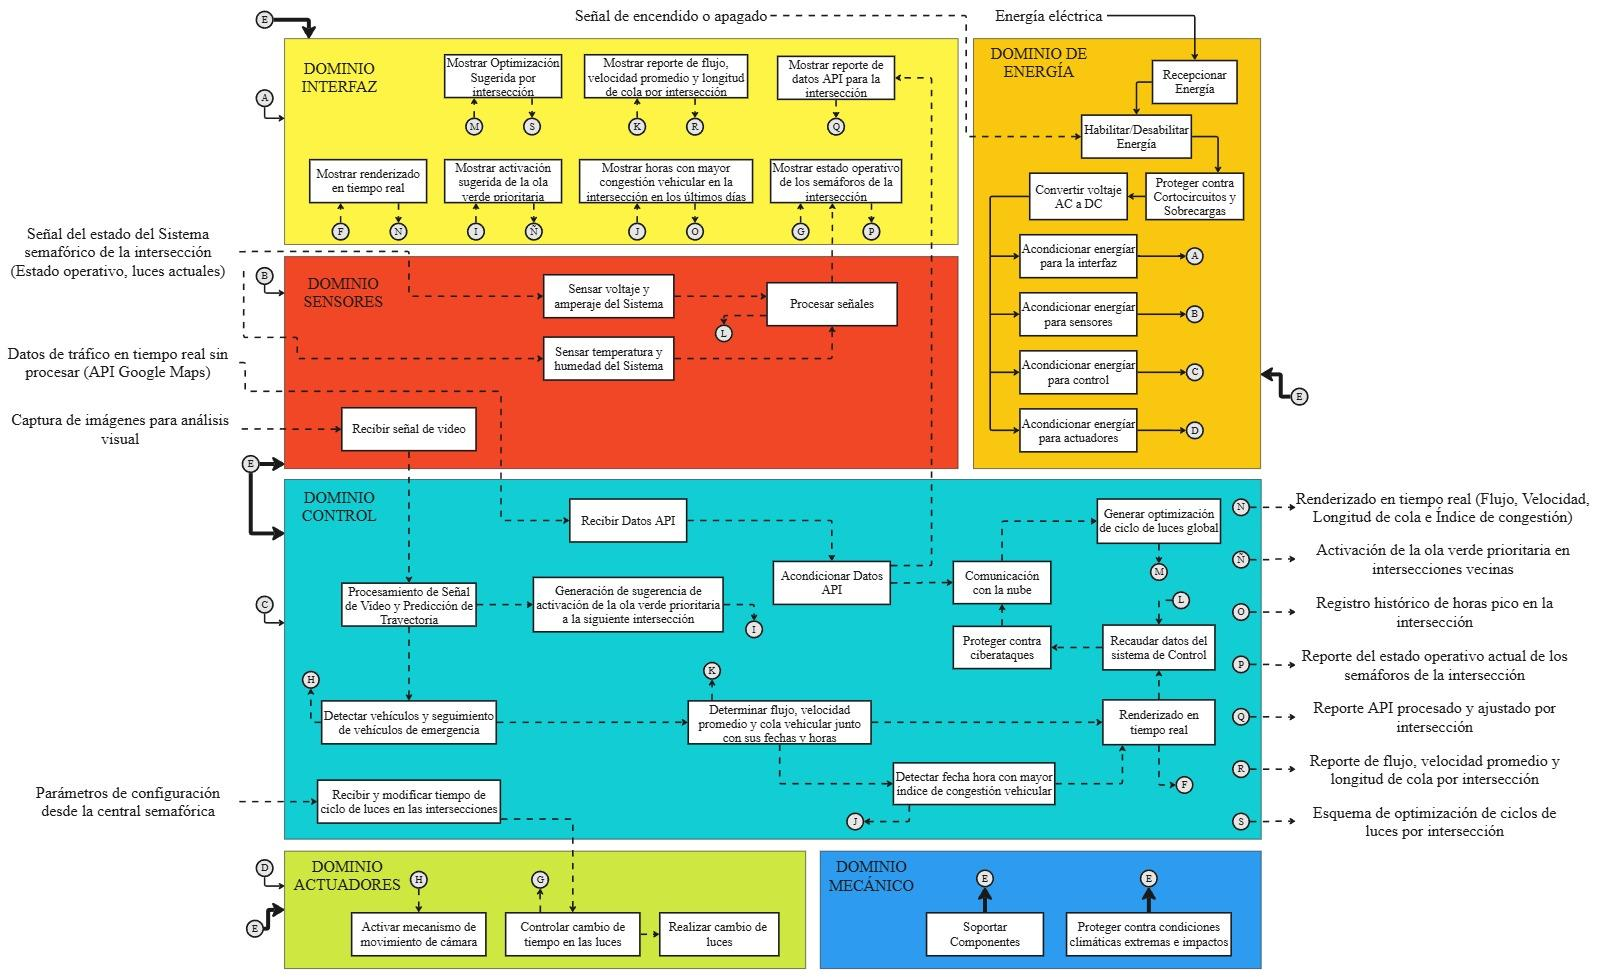
\includegraphics[width=0.92\linewidth,height=0.62\textheight,keepaspectratio]{./media/image154.jpg}
\captionof*{figure}{\small\itshape Figura 13. Estructura de funciones del sistema (Creación propia).}
\addcontentsline{lof}{figure}{Figura 13. Estructura de funciones del sistema (Creación propia).}
\label{fig:13}
\end{center}

De igual forma que con el Black List, se sigue el siguiente formato:

\begin{itemize}
\item
  Las líneas punteadas representan señales
\item
  Las líneas delgadas representan la energía
\item
  Las líneas gruesas representan la materia
\end{itemize}

\textbf{Significado de las letras:}

\begin{itemize}
\item
  \textbf{A}: Señal de acondicionar energía para la interfaz.
\item
  \textbf{B}: Señal de acondicionar energía para sensores.
\item
  \textbf{C}: Señal de acondicionar energía para control.
\item
  \textbf{D}: Señal de acondicionar energía para actuadores.
\item
  \textbf{E}: Señal mecánica de soporte y protección contra condiciones extremas e impactos.
\item
  \textbf{F}: Señal de Renderizado en tiempo real.
\item
  \textbf{G}: Señal de cambio de tiempo en las luces.
\item
  \textbf{H}: Señal de seguimiento visual continuo del vehículo de emergencia.
\item
  \textbf{I}: Señal de generación de sugerencia para la activación de la ola verde prioritaria.
\item
  \textbf{J}: Señal de índice de congestión vehicular por fecha y hora.
\item
  \textbf{K}: Señal de obtener reporte de flujo, velocidad promedio y longitud de cola por intersección.
\item
  \textbf{L}: Señal de datos acondicionados del estado del Sistema Semafórico.
\item
  \textbf{M}: Señal de generación de optimización de ciclo de luces Global.
\item
  \textbf{N}: Señal de Interfaz mostrar renderizado en tiempo real.
\item
  \textbf{Ñ}: Señal de Interfaz mostrar activación sugerida de la ola verde prioritaria.
\item
  \textbf{O}: Señal de Interfaz mostrar horas con mayor congestión vehicular en la intersección.
\item
  \textbf{P}: Señal de Interfaz mostrar estado operativo de los semáforos de la intersección.
\item
  \textbf{Q}: Señal de Interfaz mostrar reporte de datos API para la intersección.
\item
  \textbf{R}: Señal de Interfaz mostrar reporte de flujo, velocidad y longitud de cola por intersección.
\item
  \textbf{S}: Señal de Interfaz mostrar optimización sugerida por intersección.
\end{itemize}

Como se observa en la Figura 23, este sistema de control de semáforos inteligente está diseñado para optimizar el tráfico vehicular en tiempo real, gestionando tanto el control del semáforo como la energía, los sensores, los actuadores y la interfaz con el usuario.

El primer paso en el funcionamiento del sistema es la activación del mismo, asegurando que todos los componentes estén energizados. Esto se gestiona a través de una unidad que distribuye energía a las distintas partes del sistema, como la interfaz, los sensores, el control y los actuadores. Una vez que la energía está disponible, el sistema puede comenzar a recibir datos de diversas fuentes, tales como cámaras de video que monitorizan el tráfico y sensores que proporcionan información sobre la congestión vehicular y las condiciones del semáforo.

El sistema también se conecta a fuentes externas, como Google Maps, para obtener información en tiempo real sobre el flujo vehicular en la zona, lo que ayuda a ajustar los semáforos según el estado del tráfico junto con los datos provenientes de las cámaras con procesamiento digital. Con estos datos, el sistema procesa la información y toma decisiones sobre el tiempo que cada semáforo debe permanecer en verde, ajustándose a las necesidades del tráfico y priorizando a vehículos de emergencia cuando sea necesario. Además, el sistema tiene la capacidad de aprender y optimizar los ciclos de luces según las horas de mayor congestión, lo que permite mejorar la eficiencia del flujo vehicular durante el día.

Una vez que se ha determinado el tiempo necesario para cada luz, el sistema de control envía las señales de sugerencia de optimización desde la nube a la central semafórica, una vez procesada por la persona encargada esta envía una señal por NTCIP hacia el controlador donde indica la modificación del ciclo semafórico en base a la sugerencia, esta señal se procesa y va directamente a ser accionada por el actuador del semáforo, que es el encargado de ajustar físicamente las luces según las decisiones tomadas. Estos actuadores permiten que el semáforo cambie de manera dinámica, ajustando los tiempos de luz verde para facilitar el paso de vehículos, reducir los tiempos de espera y disminuir la congestión.

A lo largo de este proceso, el sistema también está protegido contra condiciones extremas, garantizando que los componentes físicos, como los actuadores y sensores, no se vean afectados por factores climáticos adversos o daños mecánicos. Además, todo el sistema está diseñado para ser accesible y monitoreado a través de una interfaz visual, que proporciona al operador información sobre el estado del semáforo, las alertas del sistema y las recomendaciones de optimización.

A continuación se explicará cada función proveniente de los dominios explicados anteriormente.

\begin{center}
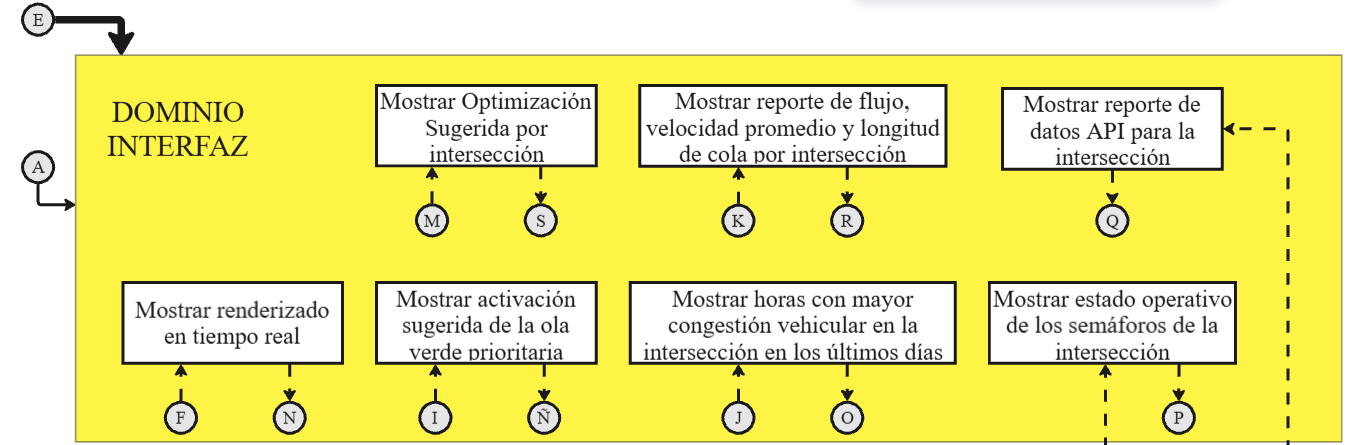
\includegraphics[width=0.92\linewidth,height=0.62\textheight,keepaspectratio]{./media/image27.png}
\captionof*{figure}{\small\itshape Figura 14. Estructura de funciones {[}Dominio Interfaz{]} (Creación propia).}
\addcontentsline{lof}{figure}{Figura 14. Estructura de funciones {[}Dominio Interfaz{]} (Creación propia).}
\label{fig:14}
\end{center}

Dominio de Interfaz:

\begin{itemize}
\item
  \textbf{Mostrar renderizado en tiempo real}:\\
  Esta función utiliza las cámaras instaladas en las intersecciones para capturar imágenes en tiempo real del tráfico vehicular. Mediante procesamiento digital de video, se extraen métricas clave como el flujo de vehículos, velocidad promedio, longitud de cola e índice de congestión.
\item
  \textbf{Mostrar optimización sugerida por intersección}:\\
  El sistema presenta las recomendaciones generadas automáticamente para la optimización de los ciclos semafóricos en cada intersección. Estas sugerencias se basan en el análisis integral de los datos de tráfico provenientes de sensores, cámaras y fuentes externas (como la API de Google Maps).
\item
  \textbf{Mostrar estado operativo de los semáforos de la intersección}:\\
  Esta interfaz muestra el estado en tiempo real de cada semáforo, color actual de la luz (rojo, verde, ámbar), estado funcional (activo, inactivo, falla detectada) y el tiempo restante en el ciclo actual. Permite al operador identificar rápidamente si alguna unidad requiere mantenimiento o intervención, facilitando el mantenimiento predictivo y la continuidad operacional.
\item
  \textbf{Mostrar reporte de flujo, velocidad promedio y longitud de cola por intersección}:\\
  Esta función muestra un reporte detallado que incluye las métricas operativas del tráfico vehicular como flujo de vehículos que atraviesan la intersección, velocidad promedio, longitud de cola en tiempo real y tendencias históricas en métricas.
\item
  \textbf{Mostrar activación sugerida de la ola verde prioritaria:}\\
  Esta función visualiza las sugerencias de activación de la ola verde prioritaria para vehículos de emergencia. Basándose en la detección mediante cámaras y sensores, el sistema propone la sincronización de semáforos en intersecciones vecinas para permitir un paso ininterrumpido. El operador puede supervisar y autorizar estas activaciones para mejorar la respuesta ante emergencias.
\item
  \textbf{Mostrar las horas con mayor congestión vehicular en la intersección en los últimos días:}\\
  Se presenta un histórico gráfico con las horas pico de congestión detectadas en la intersección, utilizando datos almacenados y procesados. Esto identifica patrones diarios y semanales, facilitando la planificación y ajuste de los ciclos semafóricos.
\item
  \textbf{Mostrar reporte de datos API para la intersección:}\\
  Esta interfaz despliega los datos de tráfico provenientes de fuentes externas, como la API de Google Maps, procesados y ajustados para la intersección específica.
\end{itemize}

\begin{center}
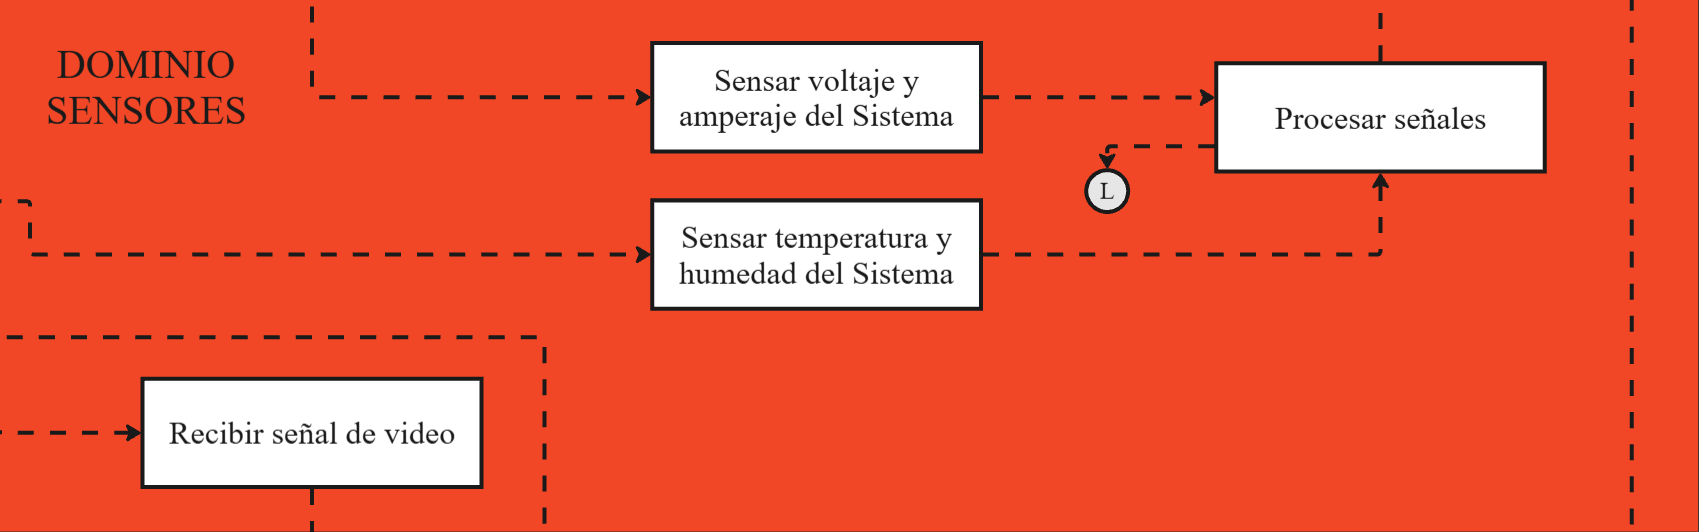
\includegraphics[width=0.92\linewidth,height=0.62\textheight,keepaspectratio]{./media/image74.png}
\captionof*{figure}{\small\itshape Figura 15. Estructura de funciones {[}Dominio de Sensores{]} (Creación propia).}
\addcontentsline{lof}{figure}{Figura 15. Estructura de funciones {[}Dominio de Sensores{]} (Creación propia).}
\label{fig:15}
\end{center}

Dominio de Sensores:

\begin{itemize}
\item
  \textbf{Recibir señal de video}:\\
  Esta función recibe las señales de vídeo en tiempo real capturadas por las cámaras instaladas en las intersecciones. Las cámaras monitorean el flujo vehicular, detectan vehículos de emergencia y capturan imágenes necesarias para calcular métricas clave como la velocidad promedio de los vehículos, la longitud de las colas y la densidad del tráfico.
\item
  \textbf{Sensar voltaje y amperaje del sistema:}\\
  Este módulo tiene la responsabilidad de monitorear continuamente los niveles de voltaje y amperaje dentro del sistema semafórico. Si se detectan fluctuaciones o anomalías en estos valores, el sistema puede activar alertas visuales.
\item
  \textbf{Sensar temperatura y humedad del sistema:\\
  }Los sensores encargados de medir la temperatura y la humedad monitorean el entorno en el que operan los equipos, asegurando que las condiciones sean óptimas para su funcionamiento. La temperatura excesiva o la alta humedad pueden afectar el rendimiento de los semáforos y los sensores, por lo que estos datos permiten al sistema adelantarse a mantenimientos necesarios.
\item
  \textbf{Procesar señales}:\\
  Esta función monitorea continuamente el estado operativo del sistema semafórico, incluyendo la funcionalidad de los semáforos, sensores, alimentación eléctrica y condiciones ambientales. A través de sensores dedicados se detectan fallas, desconexiones o anomalías.
\end{itemize}

\begin{center}
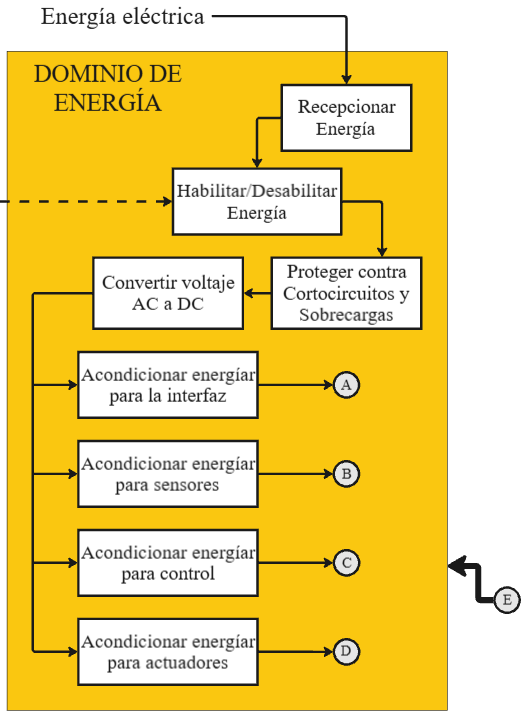
\includegraphics[width=0.92\linewidth,height=0.62\textheight,keepaspectratio]{./media/image83.png}
\captionof*{figure}{\small\itshape Figura 16. Estructura de funciones {[}Dominio de Energía{]} (Creación propia).}
\addcontentsline{lof}{figure}{Figura 16. Estructura de funciones {[}Dominio de Energía{]} (Creación propia).}
\label{fig:16}
\end{center}

Dominio de Energía:

\begin{itemize}
\item
  \textbf{Recepcionar Energía}:\\
  Esta función es responsable de recibir y gestionar la energía proveniente de la fuente principal, que proviene de la red eléctrica convencional. Se asegura que el sistema cuente con un suministro energético estable y continuo para mantener operativos todos sus componentes (sensores, actuadores, controladores, interfaz)..
\item
  \textbf{Habilitar/ Deshabilitar Energía}:\\
  Esta función controla la activación o desactivación del sistema de manera remota.
\item
  \textbf{Proteger contra Cortocircuitos y Sobrecargas:}\\
  Esta función implementa mecanismos de protección eléctrica para evitar daños en el sistema causados por condiciones anómalas en el suministro eléctrico, tales como cortocircuitos, sobrecargas o picos de tensión..
\item
  \textbf{Convertir Voltaje AC a DC}\\
  Dado que la mayoría de los componentes electrónicos del sistema operan con corriente continua (DC), esta función se encarga de convertir la energía eléctrica entrante en corriente alterna (AC) a corriente continua regulada. Utiliza fuentes de alimentación con rectificadores y reguladores de voltaje para entregar una tensión estable y adecuada a cada módulo del sistema, garantizando un funcionamiento seguro y eficiente.
\item
  \textbf{Transformar energía para la interfaz (A)}:\\
  Esta función convierte la energía que se recibe para ser utilizada específicamente por la interfaz de usuario.
\item
  \textbf{Transformar energía para sensores (B)}:\\
  Esta función es responsable de proporcionar la energía necesaria para el funcionamiento de los sensores.
\item
  \textbf{Transformar energía para control (C)}:\\
  Esta función convierte la energía para ser utilizada por el sistema de control.
\item
  \textbf{Transformar energía para actuadores(D)}:\\
  Esta función convierte la energía para ser utilizada por los actuadores del sistema.
\end{itemize}

\begin{center}
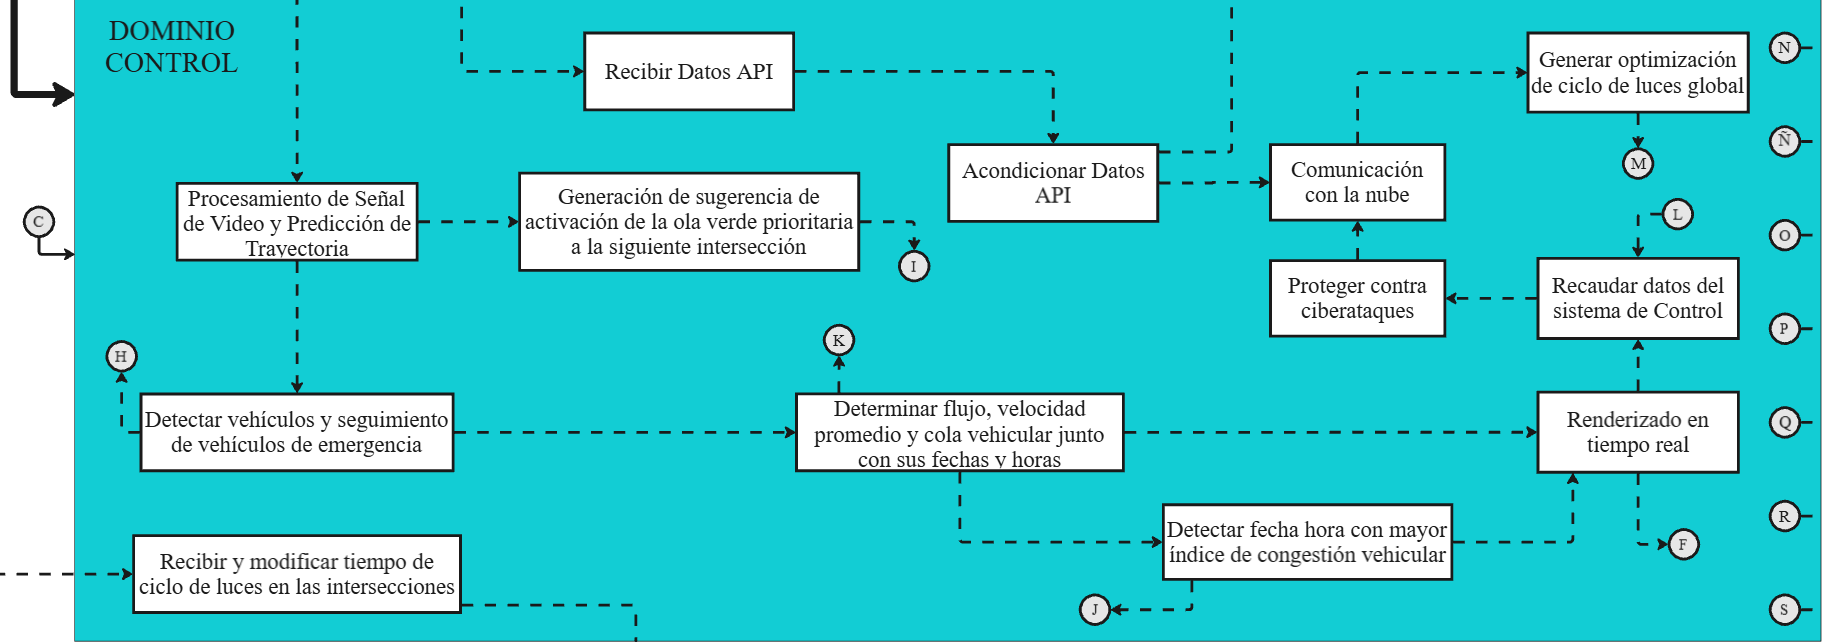
\includegraphics[width=0.92\linewidth,height=0.62\textheight,keepaspectratio]{./media/image80.png}
\captionof*{figure}{\small\itshape Figura 17. Estructura de funciones {[}Dominio de Control{]} (Creación propia).}
\addcontentsline{lof}{figure}{Figura 17. Estructura de funciones {[}Dominio de Control{]} (Creación propia).}
\label{fig:17}
\end{center}

Dominio de Control:

\begin{itemize}
\item
  \textbf{Recibir Datos API (Google Maps)}:\\
  El sistema recibe datos en tiempo real provenientes de la API de Google Maps, que proporciona información adicional sobre el estado del tráfico, condiciones viales y eventos en la zona de cada intersección. Estos datos complementan la información interna.
\item
  \textbf{Acondicionar Datos API}:\\
  Los datos crudos obtenidos de la API externa son filtrados y adaptados para ser compatibles con el sistema de control. Esto implica normalización, corrección de formatos y verificación de consistencia para asegurar que la información sobre flujo vehicular y congestión pueda integrarse efectivamente con las métricas internas del sistema. Dado que la información recibida abarca múltiples zonas y vías, esta función segmenta y distribuye los datos procesados de acuerdo a cada intersección específica. Esto permite que el control adaptativo gestione individualmente cada nodo semafórico con datos precisos y relevantes para su ubicación.
\item
  \textbf{Detectar vehículos y seguimiento de vehículos de emergencia:\\
  }A partir de la señal segmentada, esta función identifica y cuenta los vehículos presentes en la intersección, diferenciando tipos. Mediante algoritmos de reconocimiento específicos, esta función identifica vehículos de emergencia en circulación (ambulancias, bomberos, policía) y verifica que estén operativos para ser priorizados en el sistema. Una vez detectado, el sistema realiza un seguimiento constante del vehículo de emergencia para conocer su ubicación precisa y trayectoria. Esto permite anticipar su paso por las intersecciones y ajustar el control semafórico para facilitar su tránsito.
\item
  \textbf{Procesamiento de Señal de Video y Predicción de Trayectoria:\\
  }Una vez recibida la señal de video, se aplica un proceso de acondicionamiento que incluye la filtración para mejorar la calidad de la imagen, reduciendo el ruido y estabilizando la señal. Este procesamiento permite identificar y delimitar automáticamente las zonas relevantes dentro de las imágenes capturadas por las cámaras en las intersecciones, como carriles vehiculares, pasos peatonales y áreas de espera. Con base en los datos obtenidos del seguimiento de vehículos y utilizando modelos predictivos, se calcula la ruta probable de un vehículo de emergencia hacia la siguiente intersección. Este análisis permite coordinar anticipadamente la activación de la ola verde prioritaria para optimizar el flujo de tráfico garantizando además el desplazamiento ágil de los vehículos de emergencia.
\item
  \textbf{Generación de sugerencia de activación de la ola verde prioritaria a la siguiente intersección:}
\end{itemize}

Esta función se encarga de comunicar a la próxima intersección la llegada inminente del vehículo prioritario, permitiendo que el sistema se prepare para activar la ola verde y así garantizar el paso sin interrupciones. Con base en la detección y predicción de vehículos prioritarios, esta función crea recomendaciones para activar la ola verde en las intersecciones involucradas, optimizando el paso rápido y seguro del vehículo de emergencia.

\begin{itemize}
\item
  \textbf{Determinar flujo, velocidad promedio y cola vehicular junto con sus fechas y horas:\\
  }En esta función, el sistema utiliza los datos de video y sensores para la detección y extracción de características, con el fin de evaluar tres métricas en la intersección: el flujo vehicular (cantidad de vehículos que atraviesan la intersección en intervalos definidos), la velocidad promedio de los vehículos (fluidez del tráfico) y la longitud de la cola vehicular (cantidad de vehículos detenidos o esperando en la intersección durante las fases de parada de los semáforos). Esta función permite además registrar y asociar las mediciones de flujo vehicular y velocidad promedio (cuando el semáforo está en fase verde o ámbar) y las mediciones de longitud de cola vehicular (cuando el semáforo está en fase roja) con fecha y hora.
\item
  \textbf{Detectar fecha y hora con mayor índice de congestión vehicular:\\
  }Analiza los datos históricos para identificar los momentos con mayor saturación vehicular, en base a un cálculo de las variables de tráfico asignándoles pesos de relevancia.
\item
  \textbf{Renderizado en tiempo real:\\
  }Presenta en la interfaz del operador visualizaciones actualizadas al instante con los datos más relevantes: flujo, velocidad promedio, longitud de cola e índice de congestión, facilitando el monitoreo y toma de decisiones.
\item
  \textbf{Recaudar datos del sistema semafórico}:\\
  Esta función se encarga de recoger los datos de todo el sistema. Estos datos se utilizan para optimizar los ciclos de los semáforos en base a un análisis de control en la nube.
\item
  \textbf{Protección contra ciberataques}:\\
  Dada la importancia del control semafórico para la seguridad vial, esta función se enfoca en proteger el sistema contra posibles ciberataques. Esto incluye la implementación de medidas de seguridad cibernética para garantizar que los datos y el control del sistema estén protegidos de accesos no autorizados.
\item
  \textbf{Comunicación con la nube}:\\
  Esta función asegura que el sistema semafórico se comunique de manera eficiente con la nube para almacenar datos, recibir actualizaciones y sugerencias de optimización, y mantener una sincronización constante entre los distintos nodos del sistema.
\item
  \textbf{Generar optimización de ciclo de luces global:}\\
  A partir de toda la información recibida y procesada, esta función genera una propuesta de optimización global para los ciclos de luces en la red semafórica, buscando maximizar la fluidez del tráfico en toda el área de influencia.
\item
  \textbf{Recibir y modificar tiempo de ciclo de luces en las intersecciones:}\\
  Esta función recibe las señales de configuración desde la central semafórica, permitiendo que se ajusten los parámetros de los semáforos según las necesidades del operario de la municipalidad. Implementa físicamente los cambios en los tiempos de luz verde, ámbar y rojo en el controlador de cada intersección, basándose en las configuraciones recibidas y las decisiones de optimización del sistema.
\end{itemize}

\begin{center}
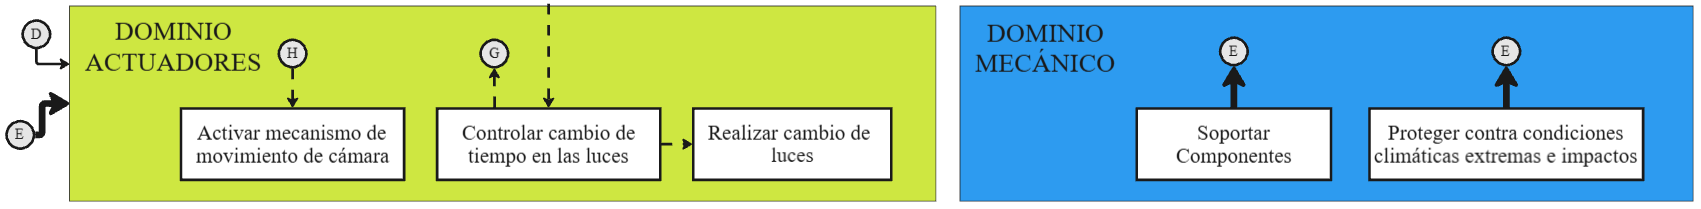
\includegraphics[width=0.92\linewidth,height=0.62\textheight,keepaspectratio]{./media/image147.png}
\captionof*{figure}{\small\itshape Figura 18. Estructura de funciones {[}Dominio Actuadores y Dominio Mecánico{]} (Creación propia).}
\addcontentsline{lof}{figure}{Figura 18. Estructura de funciones {[}Dominio Actuadores y Dominio Mecánico{]} (Creación propia).}
\label{fig:18}
\end{center}

Dominio de Actuadores:

\begin{itemize}
\item
  \textbf{Controlar cambio de tiempo en las luces:}\\
  Esta función se encarga de modificar los tiempos de los semáforos según las necesidades del tráfico. El sistema ajusta los tiempos de luz verde, ámbar o roja en función de las recomendaciones del sistema y las órdenes de la central semafórica.
\item
  \textbf{Activar mecanismo de movimiento de cámara}:\\
  Accionador que controla el movimiento de la cámara para seguir a vehículos de emergencia. Mientras el vehículo esté dentro del rango de detección, la cámara ajusta su trayectoria para mantenerlo en foco. Cuando el vehículo salga del área visual, la cámara vuelve a su posición estándar para continuar el monitoreo general. Este seguimiento permite anticipar la trayectoria del vehículo de emergencia y activar la ola verde antes de que sea detectado por la cámara de la siguiente intersección.
\item
  \textbf{Realizar cambio de luces:\\
  }Esta función se encarga de cambiar las luces del semáforo según el ciclo establecido o cuando se recibe una prioridad de emergencia, como en el caso de un vehículo de emergencia. El sistema realiza el cambio entre luces rojas, verdes y ámbar.
\end{itemize}

Dominio Mecánico:

\begin{itemize}
\item
  \textbf{Proteger contra condiciones climáticas extremas e impactos:}\\
  Esta función asegura que los componentes mecánicos y electrónicos del sistema estén protegidos frente a condiciones ambientales adversas, como lluvia, viento, temperaturas extremas, polvo, humedad y posibles impactos físicos. Incluye el diseño y selección de materiales resistentes, sellados herméticos, cubiertas y amortiguadores que permitan el funcionamiento fiable y seguro del sistema en cualquier condición meteorológica o vandalismo.
\item
  \textbf{Soportar Componentes:}\\
  Esta función se encarga de proporcionar la estructura física necesaria para alojar y mantener en posición todos los componentes del sistema semafórico, incluyendo cámaras, sensores, controladores, actuadores y la carcasa protectora. El diseño mecánico debe garantizar estabilidad, resistencia y durabilidad para que los elementos electrónicos funcionen correctamente en su ubicación específica dentro de la intersección vial.
\end{itemize}

\section{Solución óptima}\label{soluciuxf3n-uxf3ptima}

La solución óptima implementa el Concepto de Solución 3, fundamentado en un sistema de control adaptativo inteligente que se instala estratégicamente en el centro de la intersección a una altura de al menos 6,5 metros. Esta configuración centralizada permite maximizar la visibilidad y eficiencia en la captura de datos, proporcionando una cobertura completa de 180 grados de la intersección vehicular. El sistema está diseñado para operar en las condiciones ambientales adversas de Lima, caracterizadas por alta humedad y riesgo de vandalismo, por lo que se optó por un gabinete metálico protector de grado IP65. Una visualización de lo comentado se presenta en la Figura 47.

El núcleo del sistema está compuesto por un módulo IoT basado en Raspberry Pi 5, empleado como unidad de procesamiento local para adquisición de datos, visión por computadora, diagnóstico y generación de recomendaciones de control. El módulo no reemplaza al controlador semafórico existente ni asume por sí solo la autoridad final sobre los cambios de fase; su función es complementar al controlador mediante información procesada, parámetros sugeridos y alertas verificables por la central semafórica. Este módulo IoT incorpora una pantalla TFT integrada que facilita el diagnóstico del operario que vaya a revisar el controlador o el módulo IoT, mostrando únicamente el estado operativo de los semáforos y el controlador programable para propósitos de mantenimiento básico. El sistema de monitoreo energético utiliza el sensor de voltaje y corriente INA219, un componente de que opera con voltajes de medición de hasta +26V DC y corrientes de \ensuremath{\pm}3.2A con una resolución de 0.8mA, alimentándose con voltajes de 3.0V a 5.5V DC. Este sensor cuenta con un ADC interno de 12 bits, comunicación I2C y una precisión típica de \ensuremath{\pm}0.5\%, proporcionando monitoreo del consumo energético del módulo IoT semafórico para facilitar un mantenimiento preventivo.

El monitoreo de condiciones ambientales se realiza mediante el sensor de temperatura y humedad SHT31, utilizado en aplicaciones industriales de bajo costo. Este sensor opera con un rango de voltaje de 2.15V a 5.5V DC y ofrece una precisión de \ensuremath{\pm}0.3°C para temperatura y \ensuremath{\pm}2\% de humedad relativa en el rango de 20-80\% RH. Su rango operativo abarca temperaturas de -40°C a +125°C y humedad de 0-100\% RH, con comunicación I2C digital y tiempo de respuesta menor a 8 segundos. Estas especificaciones lo hacen viable en su aplicación en Lima Metropolitana por sus clásicas características.

La captura de imágenes es realizada por la cámara Raspberry Pi V2 IMX219 de 8 megapíxeles, que proporciona imágenes de 3280 x 2464 píxeles con formatos de vídeo que incluyen 1080p30 y 720p60. Esta cámara cuenta con un campo de visión de 62.2° x 48.8° e interfaz CSI (Camera Serial Interface), facilitando el análisis visual del flujo vehicular y la detección de vehículos de emergencia. El sistema está posicionado estratégicamente en el centro de la intersección sobre un soporte de dos grados de libertad controlado por dos servomotores, velocidad de operación de 0.1s/60°, torque mínimo de 2.5kg-cm, voltaje de operación de 4.8V a 6V DC y control PWM (Pulse Width Modulation). Cabe mencionar que la altura de 6.5 metros busca maximizar la visualización de la zona de interés de la intersección. La cobertura final debe verificarse mediante calibración geométrica de cámara, pruebas de campo controladas y ajuste de zonas de detección, especialmente en intersecciones con geometrías irregulares.

Para el banco de pruebas y la etapa de diseño electrónico se considera una interfaz de conmutación mediante relés de estado sólido (SSR), por su conmutación silenciosa y ausencia de desgaste mecánico. En una implementación vial real, la actuación final de las luces debe permanecer condicionada por el controlador semafórico certificado, sus enclavamientos de seguridad y las restricciones normativas aplicables. La iluminación de las luces semafóricas se plantea mediante un sistema de fibra óptica LED que permite una distribución uniforme de la luz, generando la iluminación desde la base del controlador y transmitiéndola por fibra óptica hacia los focos semafóricos, lo que resulta en un mantenimiento más accesible.

La alimentación del sistema se gestiona mediante una arquitectura que incluye llaves termomagnéticas como protección principal contra sobrecargas, disyuntores individuales para protección por circuito, una fuente conmutada para conversión AC/DC eficiente, y convertidores DC/DC para regulación de voltajes específicos para diferentes componentes. El sistema cuenta con respaldo energético mediante batería DC que garantiza continuidad operativa en caso de cortes de energía, mientras que la distribución se realiza en corriente continua para alimentar sensores, controlador y actuadores.

La comunicación entre el controlador programable y la central semafórica se establece mediante el protocolo NTCIP (National Transportation Communications for ITS Protocol) basado en TCP/IP, de igual forma entre el controlador programable y el módulo IoT. Para la comunicación entre el módulo IoT y la nube se utiliza el protocolo MQTT (Message Queuing Telemetry Transport) también basado en TCP/IP, permitiendo una transmisión de datos eficiente y segura. Todo lo mencionado priorizando la seguridad en la transmisión sin necesidad de comunicación bidireccional constante.

El procesamiento local se implementa utilizando técnicas de procesamiento de imágenes con OpenCV y YOLO ejecutándose en el Raspberry Pi, permitiendo análisis del flujo vehicular, detección automática de vehículos de emergencia, cálculo de velocidades promedio y medición de colas vehiculares. El acondicionamiento de datos se realiza mediante procesos ETL (Extract, Transform, Load) que preparan la información para su transmisión hacia la central semafórica y la nube. El análisis de datos en la nube se ejecuta en la plataforma Microsoft Azure utilizando servicios de procesamiento y almacenamiento, facilitando el análisis de datos históricos, la supervisión remota y la generación de recomendaciones de coordinación global, sin eliminar la validación local del controlador.

La seguridad cibernética se implementa mediante múltiples capas de protección que incluyen cifrado de datos para encriptación de toda la información transmitida, gestión IAM (Identity and Access Management) para control granular de accesos, y autenticación MFA (Multi-Factor Authentication) para acceso seguro al sistema. El control remoto se realiza desde una interfaz local en la central semafórica por razones de seguridad, manteniendo comunicación protegida con la nube y asegurando el aislamiento de sistemas críticos.

El sistema procesa señales de entrada que incluyen el estado del sistema semafórico de la intersección, estado operativo actual del controlador y el módulo IoT, luz semafórica activa, energía eléctrica principal, captura de imágenes para análisis visual, datos de tráfico en tiempo real provenientes de la API de Google Maps, parámetros de configuración desde la central semafórica, y señales de encendido/apagado del sistema por emergencia o mantenimiento.

La interfaz de la central semafórica proporciona funcionalidades que incluyen renderizado en tiempo real de la cámara con visualización del flujo vehicular, velocidad promedio y cola vehicular junto con hora actual y fecha, índice de congestión vehicular calculado utilizando las variables anteriores, reporte de datos de flujo, velocidad y longitud de cola históricas, interpretación amigable de datos de la API de Google Maps, sistema de activación de ola verde prioritaria cuando la cámara detecta vehículos de emergencia, visualización de horas promedio con mayor congestión vehicular en la intersección, y estado operativo completo de todos los semáforos de la intersección.

La detección de vehículos de emergencia se realiza mediante un proceso automatizado que incluye detección automática por cámara, cálculo de trayectoria accionado en los servomotores, determinación de dirección hacia hospitales o sitios de emergencia, activación de ola verde prioritaria con alcance máximo definido para no afectar el tráfico general, y consideración de la velocidad del vehículo de emergencia. El soporte de la cámara con dos grados de libertad posibilita este seguimiento.

La optimización de ciclos semafóricos se plantea como una capa de recomendación global ejecutada desde la nube, considerando datos locales de tráfico, información externa y patrones históricos de congestión. Las recomendaciones deben ser filtradas por límites de seguridad, tiempos mínimos de fase y criterios operativos de la central semafórica antes de ser aplicadas. El monitoreo continuo del sistema recolecta todos los datos con fecha y hora precisas, almacenándose en la nube. El bosquejo del diseño se aprecia en la figura 47.

\begin{center}
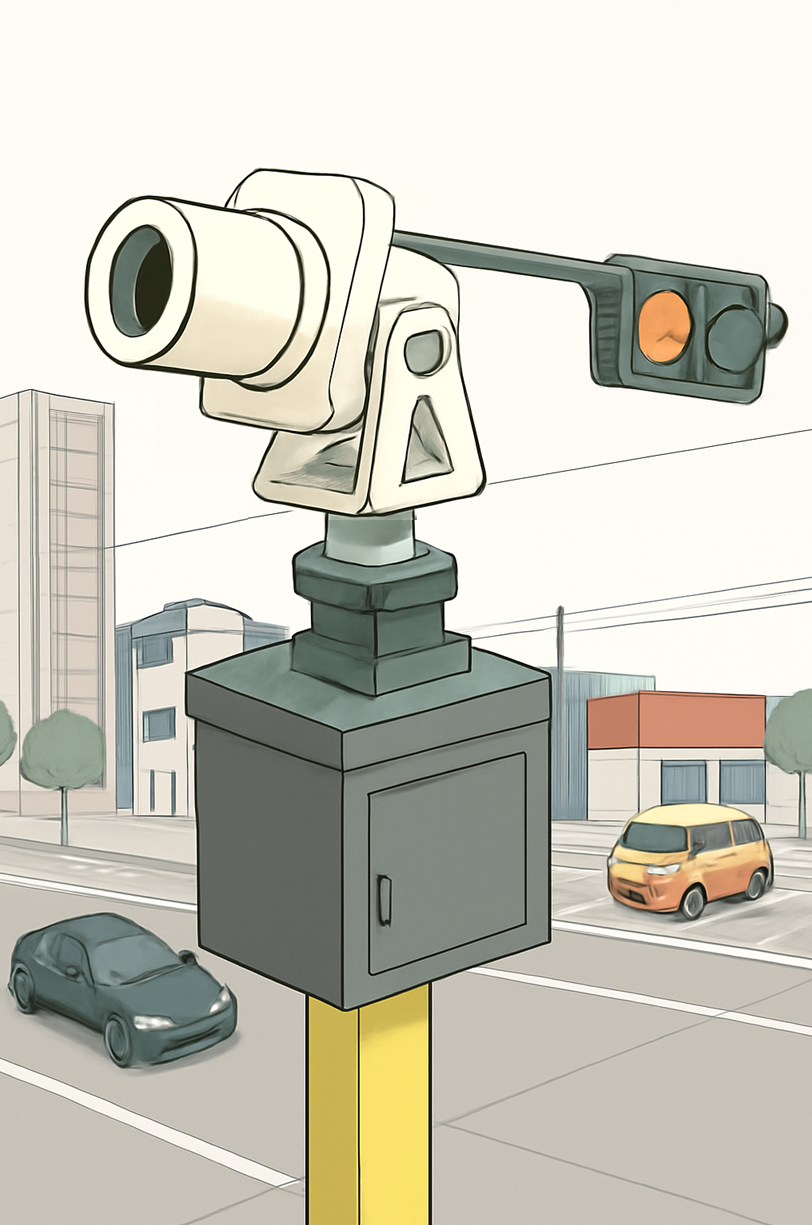
\includegraphics[width=0.92\linewidth,height=0.62\textheight,keepaspectratio]{./media/image140.png}
\captionof*{figure}{\small\itshape Figura 19. Bosquejo del diseño de la Solución Óptima (Creación propia).}
\addcontentsline{lof}{figure}{Figura 19. Bosquejo del diseño de la Solución Óptima (Creación propia).}
\label{fig:19}
\end{center}

En la figura 48 se puede apreciar el diagrama general de flujo del sistema semafórico. El controlador estándar, que actúa como el encargado de accionar directamente los semáforos, está conectado a cada uno de ellos mediante el protocolo NTCIP sobre TCP/IP, asegurando el cumplimiento de las fases y tiempos programados. A su vez, este controlador puede recibir parámetros validados o solicitudes permitidas provenientes del módulo de sensoreado y control adaptativo local, es decir, un módulo IoT instalado en la intersección, que recopila datos del entorno y se comunica con la nube mediante MQTT sobre TCP/IP.

La nube desempeña un rol de análisis adaptativo global, accediendo a los datos que le envían los distintos módulos IoT distribuidos en las intersecciones para calcular estrategias de coordinación más eficientes. Esta nube se encuentra conectada a la central semafórica supervisora, la cual también mantiene comunicación directa con el controlador programable de tráfico, recibiendo datos detallados y visuales mediante fibra óptica.

Dentro de este sistema, el módulo IoT cumple una función esencial como intermediario entre el controlador programable de tráfico y la nube, facilitando la recolección y transmisión de datos del entorno local hacia el sistema de control superior. Esta intermediación permite una comunicación fluida, incluso en contextos donde los controladores de tráfico pertenecen a diferentes marcas o plataformas, y utilizan protocolos heterogéneos. En ese sentido, la solución propuesta plantea incorporar un módulo IoT en cada intersección, el cual se comunica con el controlador programable y con la nube, sirviendo como puente para el intercambio de información, sin sustituir la lógica de control local del controlador, sino complementándola con capacidades de adaptación en tiempo real.

Esta arquitectura permite que la central semafórica tenga acceso tanto al estado operativo del controlador como a los datos procesados por la nube (Como los datos API), lo que facilita una supervisión más efectiva del comportamiento de los semáforos. Se busca mitigar de esta forma la fragmentación tecnológica existente en Lima, donde se utilizan distintas plataformas, diferentes fabricantes (SICE, SUTEC, ORIUX, SWARCO) y múltiples protocolos (AENOR, OPCT, NTCIP, BEFA), generando dificultades de interoperabilidad que el módulo IoT contribuye a solucionar mediante su rol de facilitador en la comunicación e integración del sistema.

\begin{center}
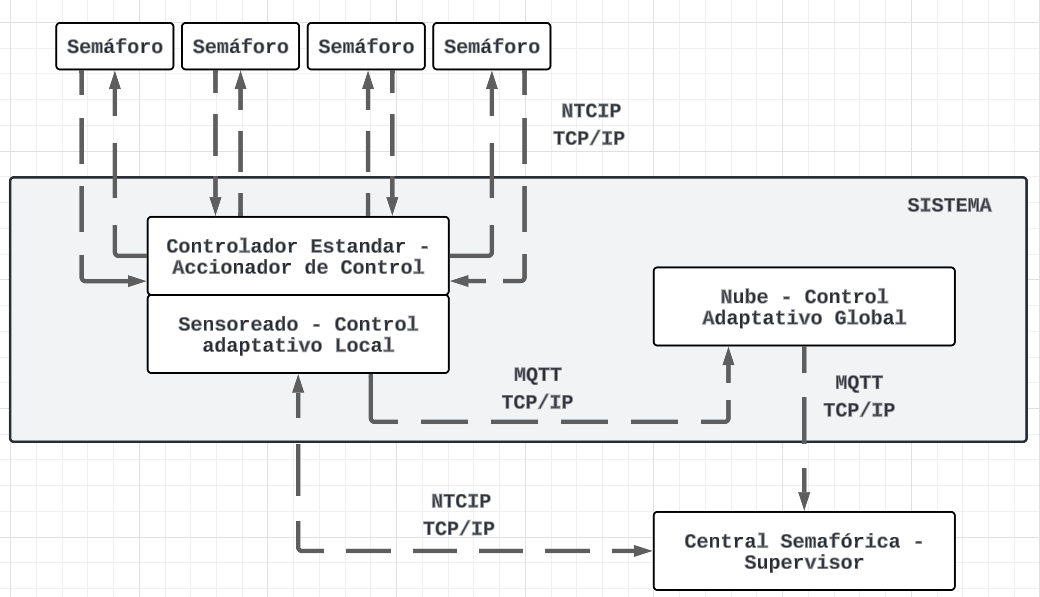
\includegraphics[width=0.92\linewidth,height=0.62\textheight,keepaspectratio]{./media/image49.png}
\captionof*{figure}{\small\itshape Figura 20. Diagrama general de flujo del sistema. (Creación propia).}
\addcontentsline{lof}{figure}{Figura 20. Diagrama general de flujo del sistema. (Creación propia).}
\label{fig:20}
\end{center}

El diagrama de flujo de la solución óptima se puede apreciar en la Figura 49, en esta se visualiza la lógica seguida por el sistema para la realización de su funcionamiento. El sistema inicia con la energización y verificación de la fuente de alimentación estable, seguido por la inicialización secuencial del controlador interno, activación de la cámara e instalación de los sensores de monitoreo ambiental y energético, así como la inicialización de los actuadores correspondientes. Una vez establecida la verificación de comunicación, el sistema entra en un bucle operativo continuo donde captura imágenes para procesamiento, detectando flujo vehicular, velocidad y colas, con las cuales calcula el índice de congestión vehicular en tiempo real. Durante este proceso, el sistema implementa una rutina de detección de vehículos de emergencia que, al ser identificados, activa el seguimiento visual para calcular la trayectoria y generar una sugerencia de activación de ola verde prioritaria adaptada a la trayectoria del vehículo. Paralelamente, el sistema ejecuta procesos de acondicionamiento de datos, cifra la información para transmisión segura hacia la nube, donde se procesa integrando datos externos para generar recomendaciones de ciclos y coordinación semafórica.

\begin{center}

\includegraphics[width=0.92\linewidth,height=0.42\textheight,keepaspectratio]{./media/image66.png}
\par\vspace{0.3em}
\begin{center}

\includegraphics[width=0.92\linewidth,height=0.62\textheight,keepaspectratio]{./media/image33.png}
\end{center}
\captionof*{figure}{\small\itshape Figura 21. Diagrama del flujo completo del sistema. (Creación propia).}
\addcontentsline{lof}{figure}{Figura 21. Diagrama del flujo completo del sistema. (Creación propia).}
\label{fig:21}
\end{center}

En la Figura 50 se define la leyenda utilizada para la estructuración del diagrama de bloque del sistema. En este se marca una separación entre las líneas de alimentación y las de señal. Además se hace una diferenciación por colores en función al dominio al que haga referencia el bloque.

\begin{center}
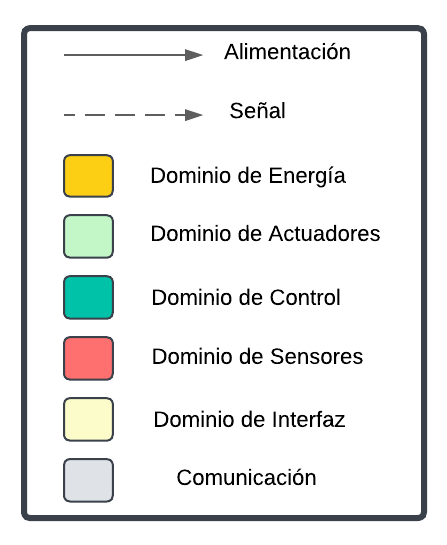
\includegraphics[width=0.92\linewidth,height=0.62\textheight,keepaspectratio]{./media/image13.png}
\captionof*{figure}{\small\itshape Figura 22. Leyenda del diagrama de bloque del sistema (Creación propia).}
\addcontentsline{lof}{figure}{Figura 22. Leyenda del diagrama de bloque del sistema (Creación propia).}
\label{fig:22}
\end{center}

En la figura 51 se observa el diagrama de bloques de la solución, en esta se evidencia la arquitectura integral del sistema de control semafórico inteligente distribuido entre procesamiento local y en la nube.

El sistema se estructura en torno a una unidad de procesamiento local basada en Raspberry Pi 5, complementada por aceleración o periféricos de procesamiento de imágenes cuando el desempeño de visión por computadora lo requiera. Este módulo se conecta con la nube Azure para análisis posterior, almacenamiento y generación de recomendaciones de coordinación semafórica. La alimentación eléctrica parte de la Red Eléctrica 220V AC, protegida por Llaves Termomagnéticas y Disyuntores, convertida mediante Fuente Conmutada AC/DC 24V, complementada con Batería DC de respaldo y Convertidores DC/DC para voltajes específicos de cada componente.

El monitoreo ambiental y energético se realiza mediante los sensores INA219 y SHT31, mientras que la captura visual se ejecuta con la Cámara V2 IMX219 montada sobre Servomotores que proporcionan seguimiento dinámico con dos grados de libertad. La comunicación opera en los siguientes niveles: protocolo NTCIP hacia la Central de Control remota, transmisión MQTT hacia la Nube Azure.

\begin{center}
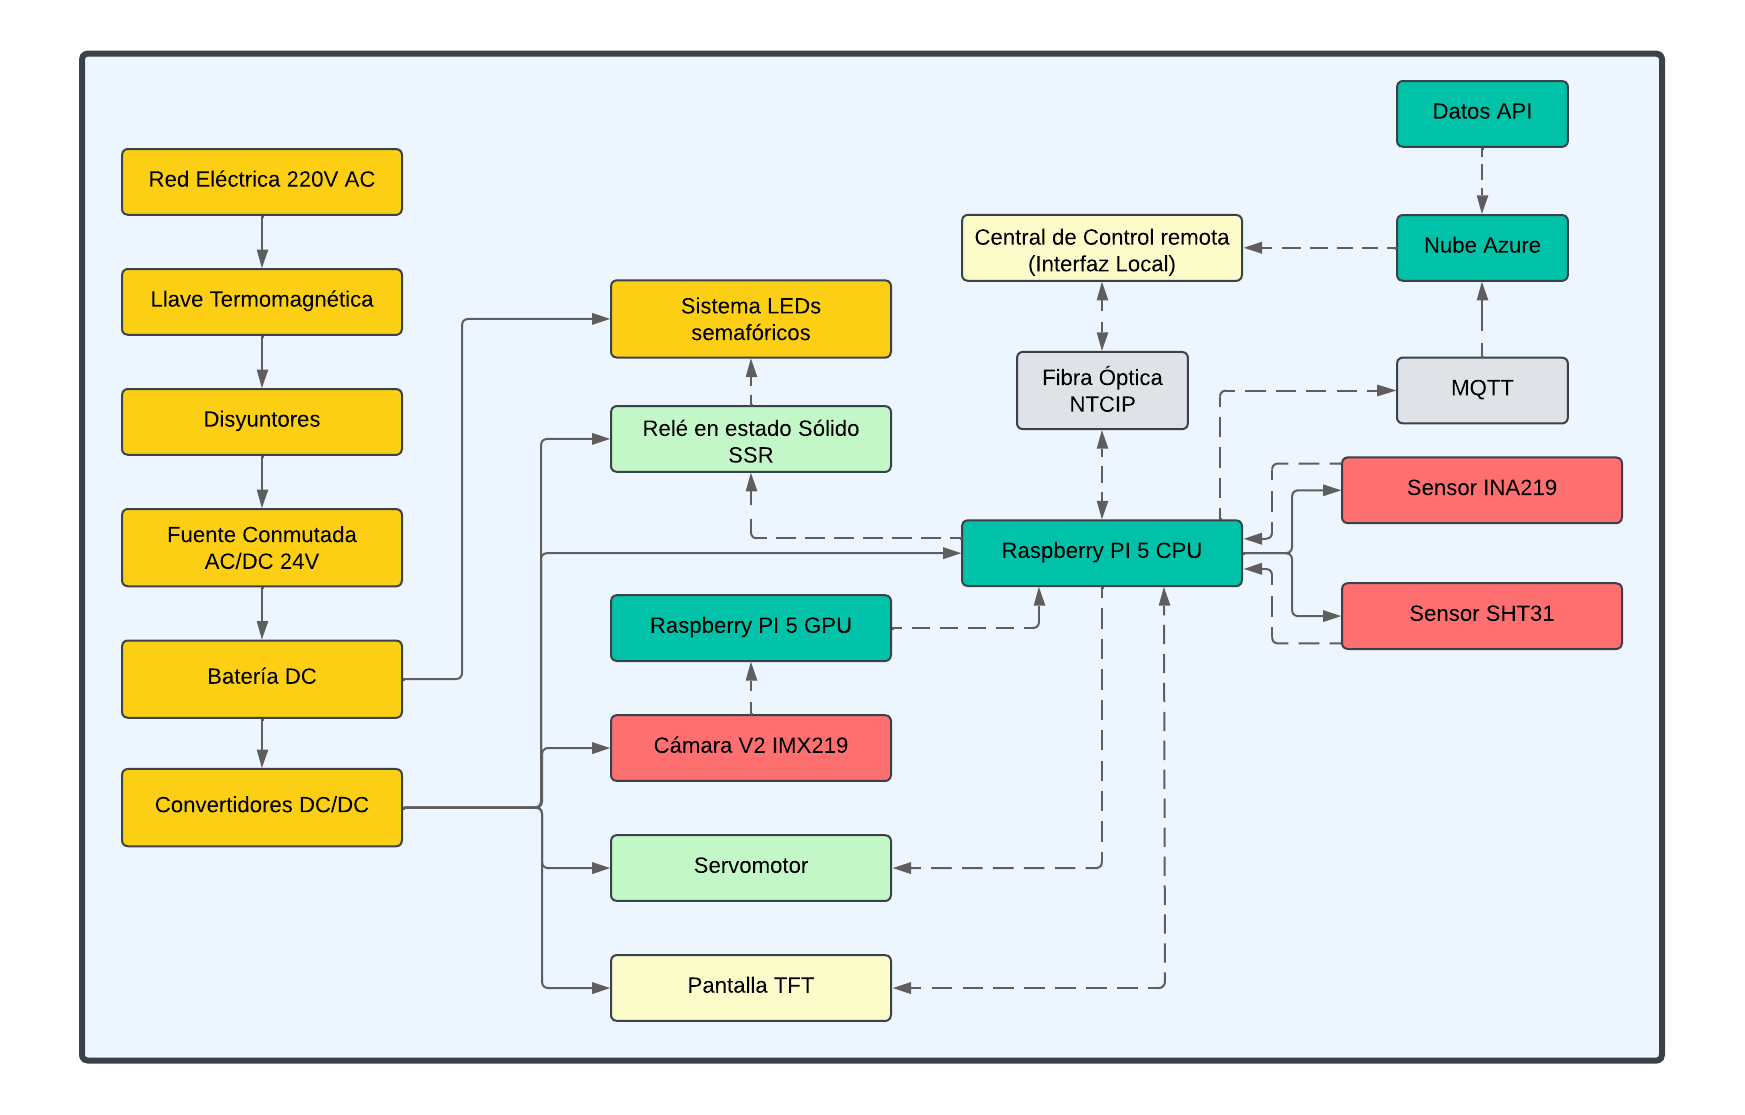
\includegraphics[width=0.92\linewidth,height=0.62\textheight,keepaspectratio]{./media/image151.png}
\captionof*{figure}{\small\itshape Figura 23. Diagrama de bloque del sistema (Creación propia).}
\addcontentsline{lof}{figure}{Figura 23. Diagrama de bloque del sistema (Creación propia).}
\label{fig:23}
\end{center}

\chapter{DISEÑO ELECTRÓNICO DEL SISTEMA}\label{capuxedtulo-4-diseuxf1o-electruxf3nico-del-sistema}

\section{Componentes electrónicos}\label{componentes-electruxf3nicos}

\subsection{Sensores}\label{sensores}

\textbf{4.1.1.1 Sensor de Temperatura}

Para la medición de temperatura del sistema se evaluaron tres opciones de sensores considerando criterios de precisión y rango. Se evaluó el DS18B20, DHT22 y el LM35, como se observa en la tabla 4.1.

Se seleccionó el módulo sensor digital DS18B20 para el sistema semafórico debido a su escalabilidad mediante el protocolo OneWire, que permite conectar múltiples sensores a un solo pin GPIO de la Raspberry Pi; su inmunidad al ruido eléctrico, esencial en entornos con interferencias electromagnéticas; su identificación única por hardware, que posibilita monitorear varios puntos críticos sin ambigüedad; la disponibilidad de versiones impermeables, adecuadas para condiciones adversas y el hecho de que no requiere un convertidor ADC externo, lo que simplifica el diseño y reduce posibles puntos de falla.

Se seleccionó el módulo sensor digital DS18B20, el cual utiliza el protocolo de comunicación OneWire para transmitir lecturas de temperatura de manera digital. Este sensor proporciona mediciones precisas en un rango que va desde -55°C hasta +125°C, con una resolución configurable entre 9 y 12 bits, lo que permite ajustar el balance entre velocidad de lectura y precisión según las necesidades del sistema.

El DS18B20 es un sensor termistor que convierte la temperatura medida directamente en una señal digital, eliminando la necesidad de conversores analógico-digitales externos. Cada sensor cuenta con un código único de 64 bits grabado en fábrica, lo que permite identificar individualmente múltiples dispositivos conectados al mismo bus de datos. Más datos en la tabla 4.2 de Anexos.

\begin{center}
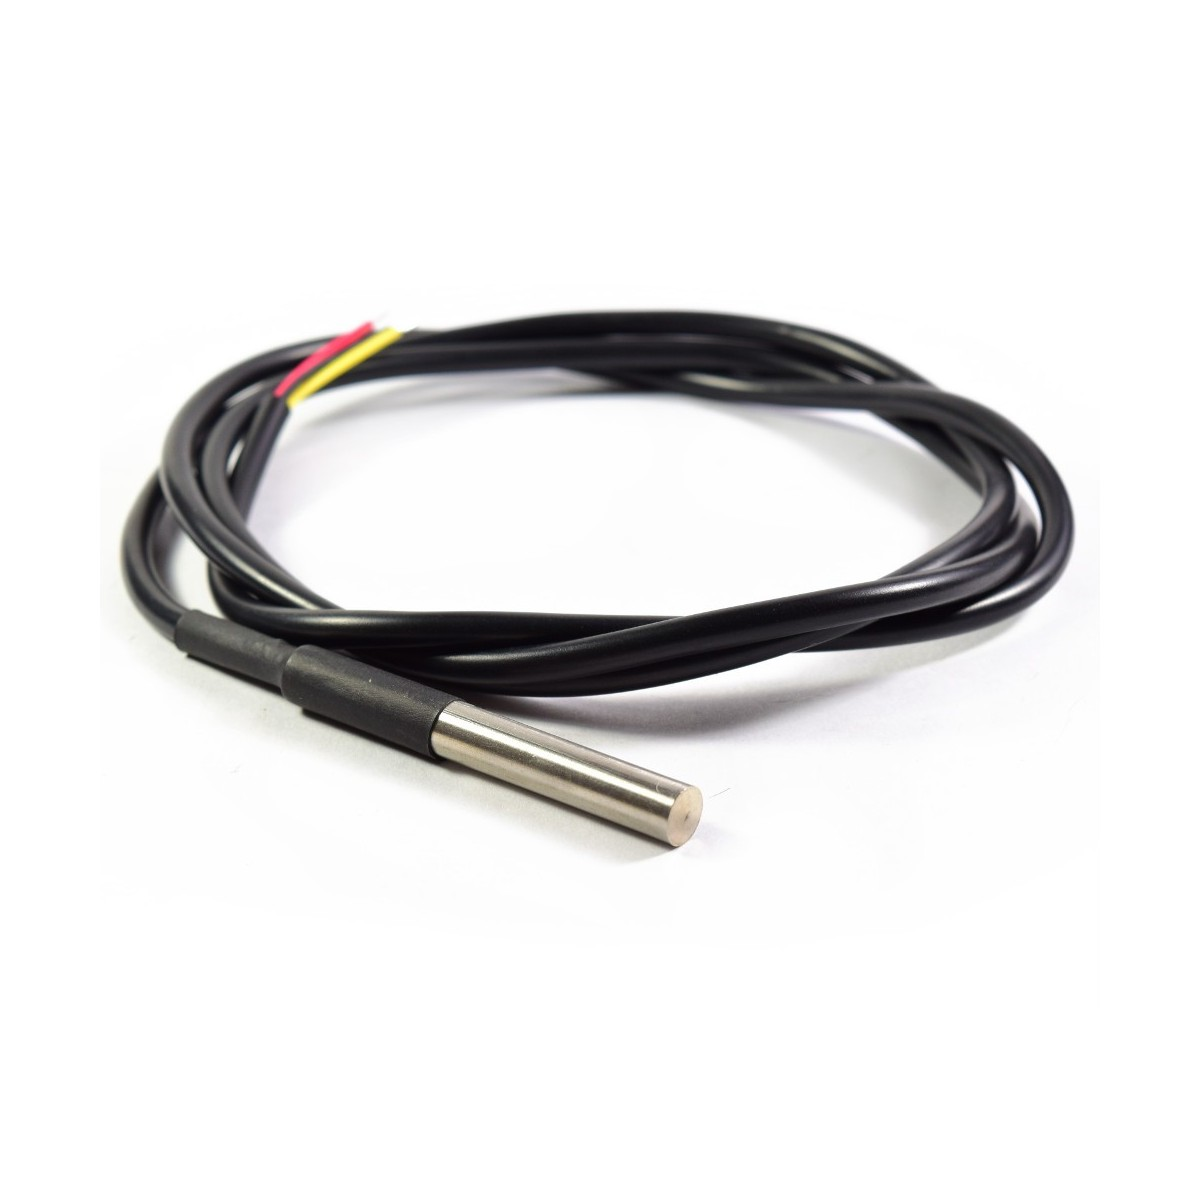
\includegraphics[width=0.92\linewidth,height=0.62\textheight,keepaspectratio]{./media/image89.png}
\captionof*{figure}{\small\itshape Figura 24. Sensor DS18B20}
\addcontentsline{lof}{figure}{Figura 24. Sensor DS18B20}
\label{fig:24}
\end{center}

La elección del sensor DS18B20 sobre otras alternativas como el DHT22 o sensores analógicos tipo LM35 se fundamenta en varios criterios técnicos relevantes para el sistema semafórico propuesto. En primer lugar, el protocolo OneWire permite conectar múltiples sensores utilizando únicamente un pin GPIO de la Raspberry Pi, lo que optimiza el uso de recursos del microcontrolador y simplifica el cableado dentro del gabinete. A diferencia de los sensores analógicos que requieren un ADC externo y sensores como el DHT22 que ocupan un pin por dispositivo, el DS18B20 puede escalar fácilmente para monitorear varios puntos críticos como la fuente de alimentación, el compartimento del procesador y el área de los relés de control.

Adicionalmente, la comunicación digital del DS18B20 proporciona inmunidad al ruido eléctrico, aspecto crucial en un entorno donde operan relés, contactores y otros dispositivos que generan interferencias electromagnéticas.

La precisión de \ensuremath{\pm}0.5°C en el rango operativo típico (-10°C a +85°C) resulta más que suficiente para detectar condiciones de sobrecalentamiento que pudieran comprometer la estabilidad del sistema. Por otro lado, la disponibilidad de versiones impermeables con encapsulado de acero inoxidable permite instalar sensores en condiciones irregulares.

\begin{center}
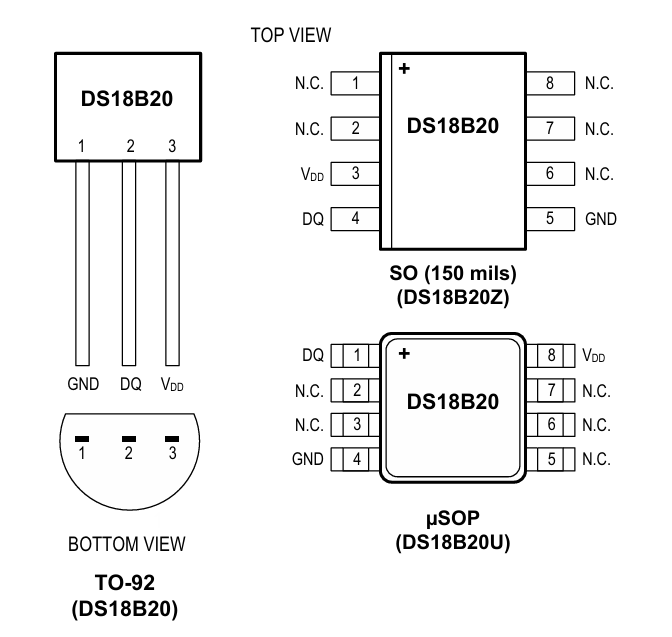
\includegraphics[width=0.92\linewidth,height=0.62\textheight,keepaspectratio]{./media/image120.png}
\captionof*{figure}{\small\itshape Figura 25. Conexiones del sensor DS18B20}
\addcontentsline{lof}{figure}{Figura 25. Conexiones del sensor DS18B20}
\label{fig:25}
\end{center}

\textbf{Limitaciones y Consideraciones}

El sensor DS18B20 requiere una resistencia pull-up externa de 4.7k\ensuremath{\Omega} conectada entre la línea de datos y el voltaje de alimentación para garantizar una comunicación estable con la Raspberry Pi. Es necesario habilitar el protocolo OneWire en la Raspberry Pi mediante la configuración del archivo /boot/config.txt, proceso que se detallará en la sección de programación del sistema.

\textbf{4.1.1.2 Sensor de Corriente}

Para la medición de corriente en el sistema semafórico se evaluaron tres alternativas tecnológicas considerando criterios de precisión, rango de medición, compatibilidad con corriente continua (DC) y alterna (AC), así como la seguridad eléctrica. Los sensores evaluados fueron el WCS1600 (efecto Hall), el ACS712 (sensor shunt) y un transformador de corriente (CT), como se muestra en la Tabla 4.3.

Para el monitoreo de corriente eléctrica se implementó el sensor WCS1600, un dispositivo que utiliza el efecto Hall para medir corrientes tanto de corriente continua (DC) como de corriente alterna (AC) sin contacto directo con el conductor. Este sensor puede detectar corrientes de hasta \ensuremath{\pm}100A en DC y 70A RMS en AC, cubriendo ampliamente los requerimientos del sistema semafórico donde las cargas típicas no superan los 10-15A por fase.

El principio de funcionamiento del WCS1600 se basa en el efecto Hall, donde un campo magnético generado por la corriente que atraviesa el conductor produce un voltaje proporcional en un semiconductor situado perpendicularmente. Este voltaje es amplificado y linearizado por un circuito integrado interno, generando una salida analógica que varía entre 0.3V y 4.7V, donde 2.5V representa corriente cero. La arquitectura del sensor incorpora compensación térmica automática mediante un circuito integrado que ajusta la respuesta del sensor ante variaciones de temperatura ambiente, manteniendo la precisión de medición en un rango operativo de -20°C a 125°C. Más datos en la tabla 4.4 de Anexos.

\begin{center}
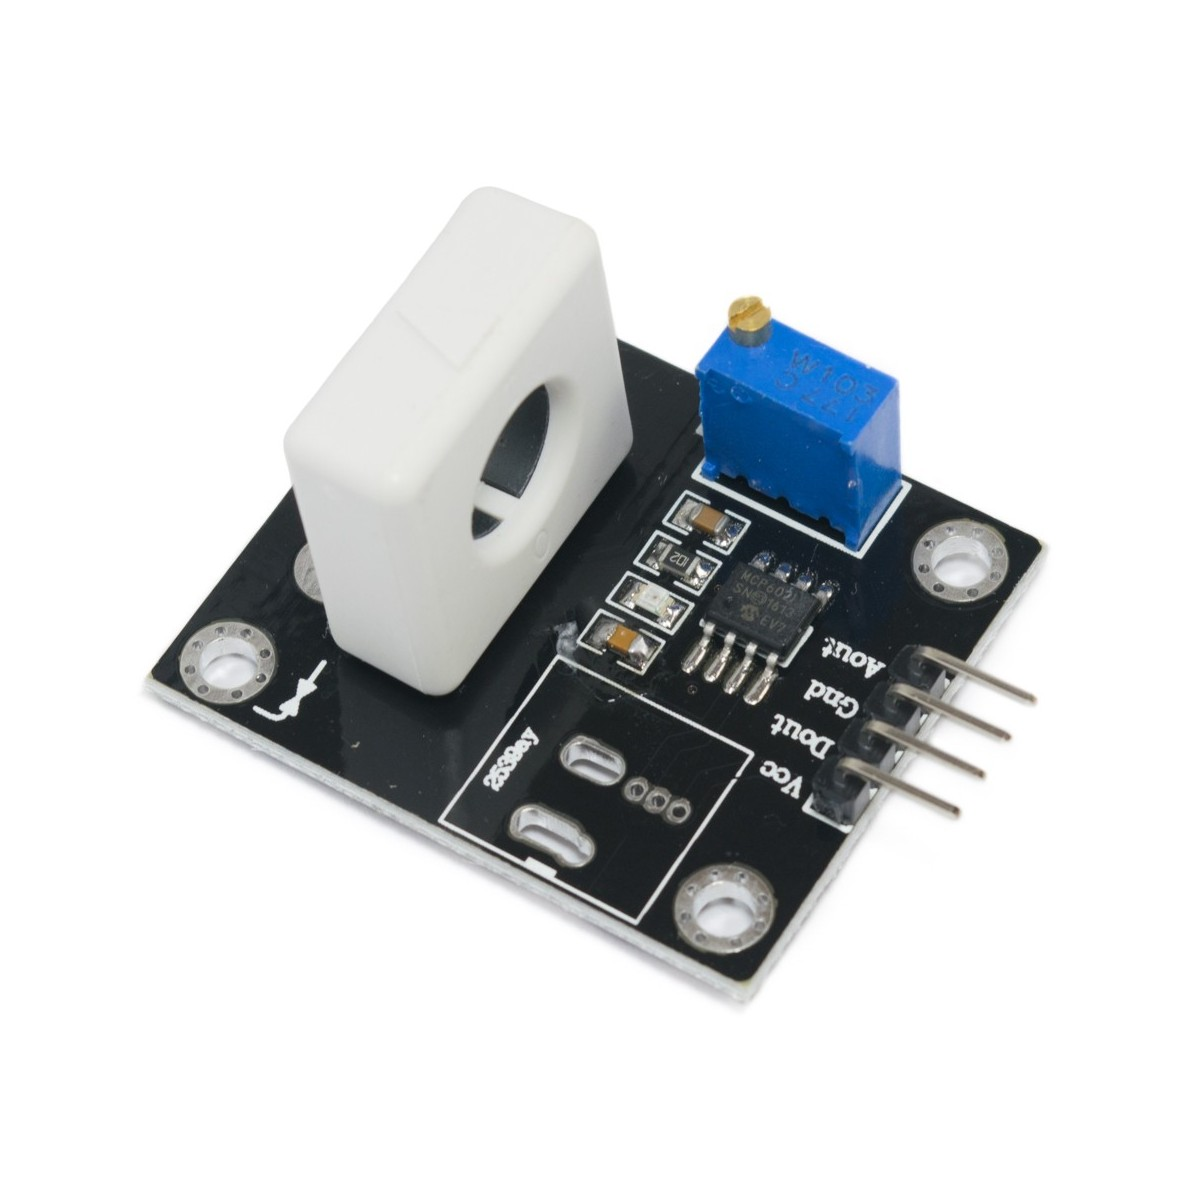
\includegraphics[width=0.92\linewidth,height=0.62\textheight,keepaspectratio]{./media/image75.png}
\captionof*{figure}{\small\itshape Figura 26. Módulo sensor WCS1600}
\addcontentsline{lof}{figure}{Figura 26. Módulo sensor WCS1600}
\label{fig:26}
\end{center}

La selección del sensor WCS1600 frente a alternativas como sensores resistivos tipo shunt o transformadores de corriente (CT) se sustenta en características técnicas específicas del sistema semafórico. El aislamiento galvánico inherente al principio del efecto Hall elimina cualquier conexión eléctrica directa entre el circuito de medición y el circuito de potencia, proporcionando seguridad tanto para el usuario como para la Raspberry Pi en caso de fallas en la instalación eléctrica. A diferencia de los sensores tipo shunt que disipan energía en forma de calor proporcional al cuadrado de la corriente medida, el WCS1600 no introduce pérdidas en el circuito de potencia, mejorando la eficiencia energética global del sistema.

La capacidad de medir tanto corriente alterna como continua con el mismo dispositivo simplifica el diseño del sistema, especialmente considerando que se contará con componentes DC. El diámetro del orificio de 9mm permite el paso de conductores AWG hasta calibre 8, suficiente para las corrientes manejadas en intersecciones semafóricas típicas.

La conexión del WCS1600 a la Raspberry Pi 5 requiere un conversor analógico-digital externo, ya que este modelo de Raspberry Pi no incluye ADC integrado. Para esta aplicación se utiliza el chip MCP3008, un ADC de 10 bits con 8 canales de entrada que se comunica mediante el protocolo SPI. El sensor WCS1600 se alimenta con una fuente externa de 5V para evitar sobrecargar la salida de 5V de la Raspberry Pi. La conversión del voltaje analógico leído por el ADC a corriente real se realiza mediante la fórmula I = (Vout - 2.5) \ensuremath{\times} 45.4545, donde I representa la corriente en amperios y Vout el voltaje de salida del sensor.

\begin{center}
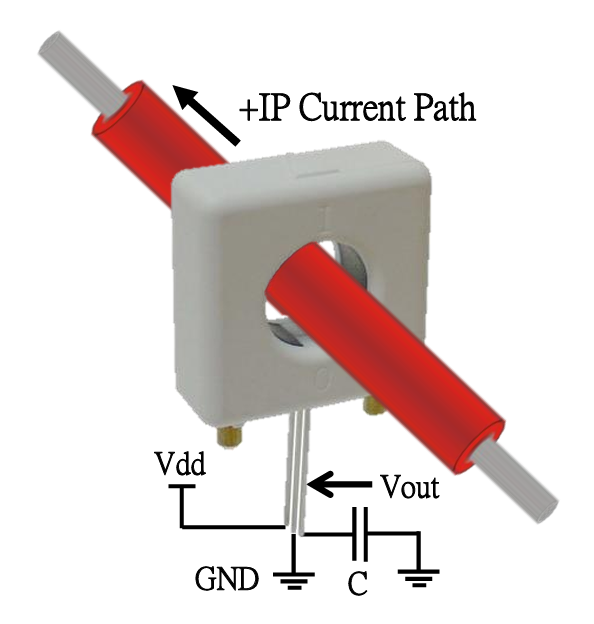
\includegraphics[width=0.92\linewidth,height=0.62\textheight,keepaspectratio]{./media/image28.png}
\captionof*{figure}{\small\itshape Figura 27. Conexión y funcionamiento del sensor WCS1600}
\addcontentsline{lof}{figure}{Figura 27. Conexión y funcionamiento del sensor WCS1600}
\label{fig:27}
\end{center}

\textbf{Limitaciones y Consideraciones}

Es importante que el conductor que transporta la corriente a medir atraviese completamente el orificio central del sensor para obtener lecturas precisas, y solo debe pasar un conductor por vez para evitar interferencias magnéticas entre fases.

\textbf{4.1.1.3 Sensor de Presencia}

Para la detección de presencia vehicular se evaluaron tres tecnologías considerando rango de detección, inmunidad a interferencias ambientales, precisión y facilidad de integración, estas son el URM06, el HC-SR04 y el Sensor Infrarrojo (PIR/IR). Comparación en la Tabla 4.5 de Anexos.

Para la detección de presencia vehicular en aproximación al semáforo se seleccionó el sensor ultrasónico URM06 con interfaz UART, el cual ofrece capacidad de detección en un rango de 20cm hasta 10 metros. Este sensor emplea tecnología ultrasónica de haz estrecho que emite pulsos de ultrasonido a 40kHz y mide el tiempo que tarda el eco en regresar, calculando la distancia al objeto mediante la fórmula d = (v \ensuremath{\times} t) / 2. El URM06 se diferencia de otros sensores ultrasónicos convencionales por su diseño de haz estrecho, que concentra la energía acústica en un ángulo de aproximadamente 15 grados. Esta característica reduce las detecciones falsas causadas por objetos laterales o reflexiones en superficies, problema común en el sensor HC-SR04. Datos en la tabla 4.6 de Anexos.

\begin{center}
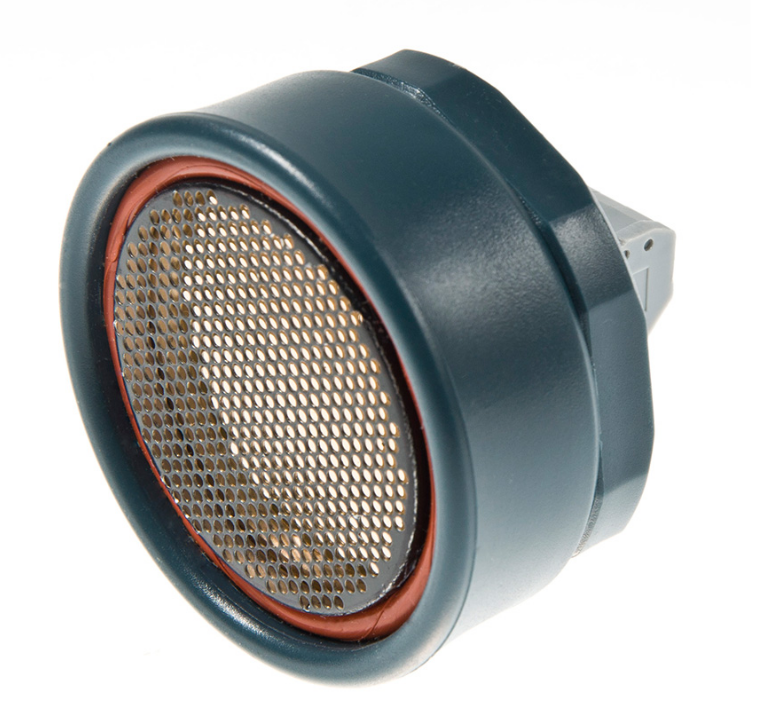
\includegraphics[width=0.92\linewidth,height=0.62\textheight,keepaspectratio]{./media/image150.png}
\captionof*{figure}{\small\itshape Figura 28. Sensor de Presencia URM06}
\addcontentsline{lof}{figure}{Figura 28. Sensor de Presencia URM06}
\label{fig:28}
\end{center}

La decisión de implementar el sensor URM06 en lugar de alternativas más económicas como el HC-SR04 o sensores infrarrojos se fundamenta en su falta de interferencia por luz solar.

La selección específica de la interfaz UART sobre las alternativas analógica, PULSE o RS485 es debido a que la interfaz UART proporciona comunicación serial asíncrona directa con el puerto serial del microcontrolador, permitiendo enviar comandos al sensor y recibir mediciones de distancia en formato digital sin necesidad de componentes adicionales.

\begin{center}
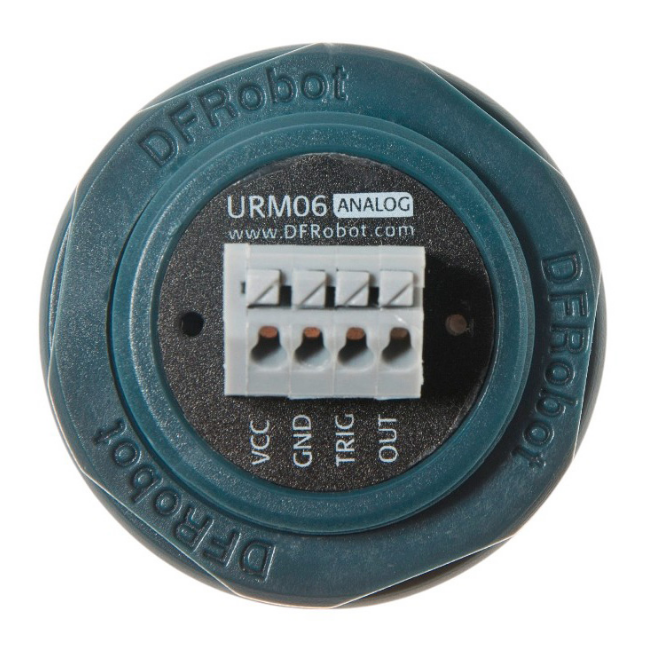
\includegraphics[width=0.92\linewidth,height=0.62\textheight,keepaspectratio]{./media/image15.png}
\captionof*{figure}{\small\itshape Figura 29. Conexión del Sensor URM06\textbf{.}}
\addcontentsline{lof}{figure}{Figura 29. Conexión del Sensor URM06\textbf{.}}
\label{fig:29}
\end{center}

\textbf{Limitaciones y Consideraciones}

Las superficies que absorben sonido, como textiles o materiales porosos, pueden atenuar significativamente el eco retornado, reduciendo el rango efectivo de detección o generando lecturas erróneas.

\textbf{4.1.1.4 Cámara Domo Fijo}

Para el sistema de videovigilancia y análisis de tráfico vehicular se evaluaron cuatro configuraciones de cámaras considerando resolución, protección ambiental, capacidad nocturna y compatibilidad con procesamiento de visión por computadora. Estas son: Cámara tipo domo, PTZ, IP y Bullet. Comparación en la tabla 4.7 de Anexos.

Para el sistema de videovigilancia y análisis de tráfico vehicular se implementó la cámara tipo domo DS-2CE57H0T-VPITF de Hikvision, que ofrece captura de video de 5 megapíxeles con tecnología EXIR 2.0 para visión nocturna efectiva. Este dispositivo proporciona resolución máxima de 2560\ensuremath{\times}1944 píxeles a 20 fotogramas por segundo, suficiente para aplicaciones de visión por computadora que requieren identificar y rastrear vehículos en la intersección semafórica. La tecnología EXIR 2.0 (Extended Infrared) implementada en esta cámara distribuye uniformemente la iluminación infrarroja en un área específica, eliminando los problemas de sobreexposición central, característica fundamental para mantener la capacidad de detección vehicular durante la noche. El alcance efectivo de la iluminación infrarroja alcanza aproximadamente 20 metros, cubriendo completamente una intersección típica de dos carriles por sentido. Datos en la tabla 4.8 de Anexos.

\begin{center}
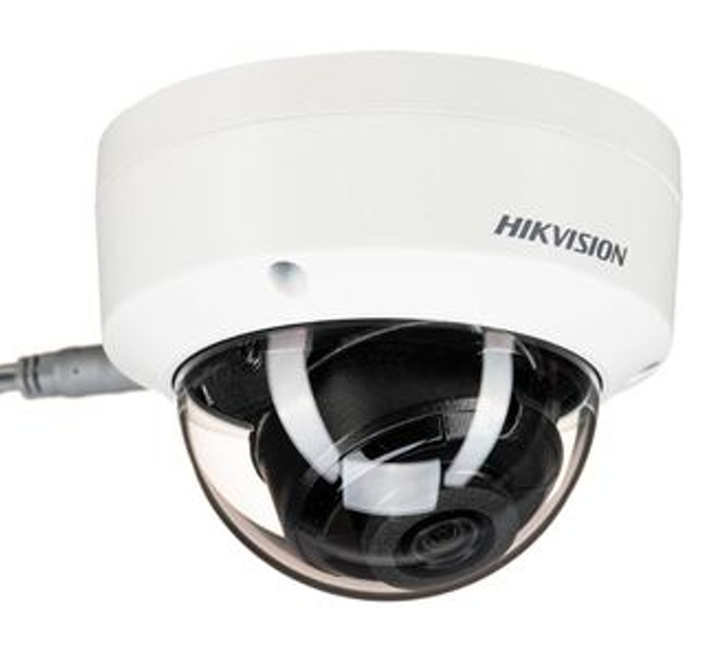
\includegraphics[width=0.92\linewidth,height=0.62\textheight,keepaspectratio]{./media/image110.png}
\captionof*{figure}{\small\itshape Figura 30. Cámara DS-2CE57H0T-VPITF}
\addcontentsline{lof}{figure}{Figura 30. Cámara DS-2CE57H0T-VPITF}
\label{fig:30}
\end{center}

\begin{center}
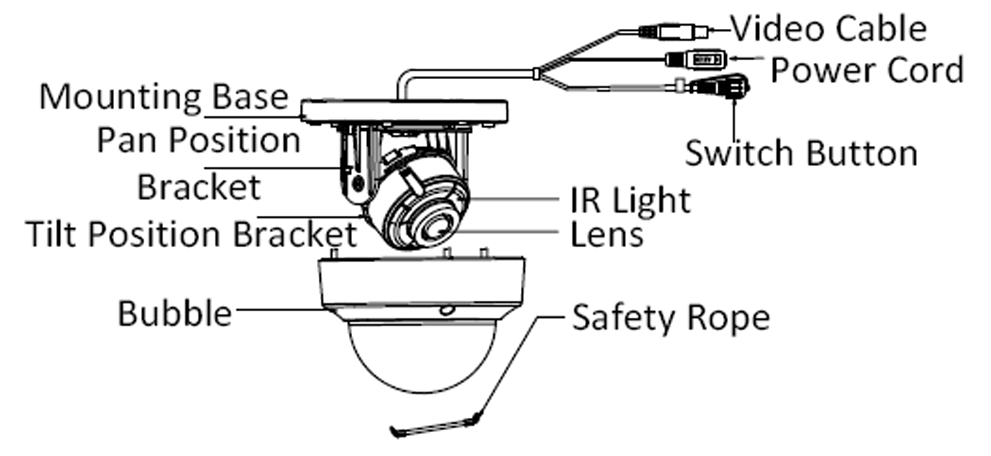
\includegraphics[width=0.92\linewidth,height=0.62\textheight,keepaspectratio]{./media/image93.png}
\captionof*{figure}{\small\itshape Figura 31. Conexión de la Cámara DS-2CE57H0T-VPITF}
\addcontentsline{lof}{figure}{Figura 31. Conexión de la Cámara DS-2CE57H0T-VPITF}
\label{fig:31}
\end{center}

La elección de esta cámara domo fija sobre alternativas como cámaras PTZ (Pan-Tilt-Zoom) motorizadas, cámaras IP estándar o cámaras tipo bullet se sustenta en múltiples criterios técnicos y operativos específicos del sistema semafórico adaptativo. La certificación IP67 garantiza protección completa contra ingreso de polvo y resistencia a inmersión temporal en agua, característica esencial considerando la exposición continua a lluvia, humedad y contaminación ambiental propia de intersecciones urbanas. La clasificación IK10 indica resistencia a impactos mecánicos de hasta 20 joules, equivalente al impacto de una masa de 5kg cayendo desde 40cm, protegiendo el equipo contra vandalismo y proyectiles accidentales.

Aunque se trata de una cámara de posición fija sin capacidad de movimiento motorizado interno, su integración con el sistema de rieles externo proporciona capacidad de reposicionamiento mecánico para cubrir diferentes ángulos de la intersección según sea necesario. El diseño tipo domo dificulta determinar visualmente hacia dónde apunta la lente, proporcionando cierto elemento de discreción operativa y reduciendo el incentivo para intentos de evadir la detección mediante posicionamiento estratégico de vehículos.

La tasa de 20 fotogramas por segundo proporciona fluidez suficiente para rastrear vehículos en movimiento sin las demandas computacionales de 30 o 60 fps utilizados en aplicaciones de vigilancia de alta velocidad. Esta configuración permite a la Raspberry Pi procesar cada cuadro con los algoritmos YOLO de detección de objetos sin acumular retraso entre la captura y el análisis. El peso de la cámara DS-2CE57H0T-VPITF es de 362 gramos.

\begin{center}
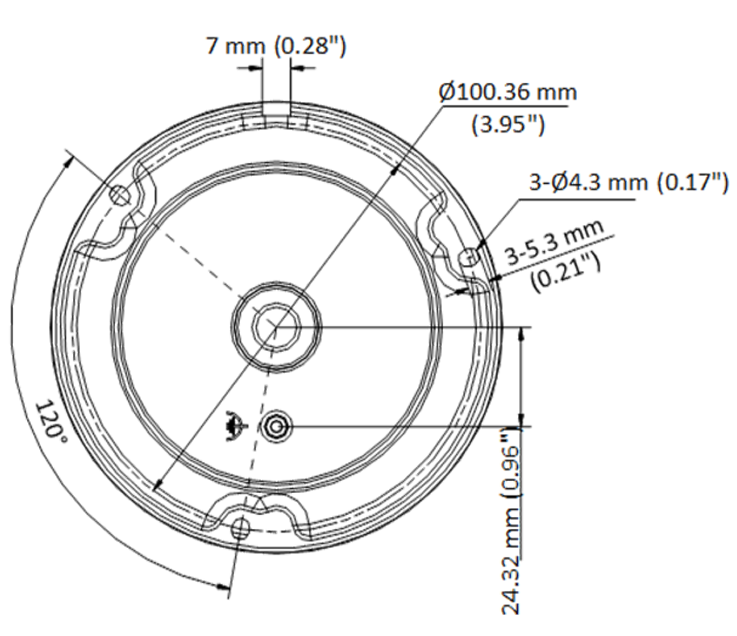
\includegraphics[width=0.92\linewidth,height=0.62\textheight,keepaspectratio]{./media/image60.png}
\captionof*{figure}{\small\itshape Figura 32. Dimensiones de la Cámara DS-2CE57H0T-VPITF}
\addcontentsline{lof}{figure}{Figura 32. Dimensiones de la Cámara DS-2CE57H0T-VPITF}
\label{fig:32}
\end{center}

La cámara DS-2CE57H0T-VPITF utiliza salida de video HD-TVI (High Definition Transport Video Interface), un estándar desarrollado específicamente para transmitir video de alta definición sobre cable coaxial tradicional. Este formato resulta incompatible directamente con las interfaces de entrada de la Raspberry Pi, que incluyen puertos USB, HDMI de entrada (solo en algunos modelos), y la interfaz CSI diseñada para cámaras de placa específicas. Para resolver esta incompatibilidad se implementa un convertidor de video 4-en-1 AHD/CVBS/CVI/TVI a USB, dispositivo que actúa como puente de comunicación:

\begin{center}
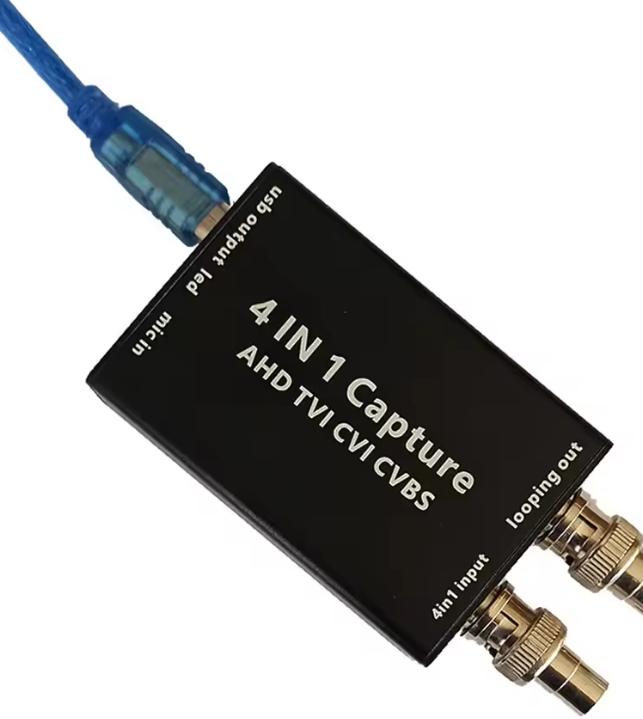
\includegraphics[width=0.92\linewidth,height=0.62\textheight,keepaspectratio]{./media/image85.png}
\captionof*{figure}{\small\itshape Figura 33. Convertidor de vídeo 4 en 1 AHD CVBS CVI TVI a USB}
\addcontentsline{lof}{figure}{Figura 33. Convertidor de vídeo 4 en 1 AHD CVBS CVI TVI a USB}
\label{fig:33}
\end{center}

La Raspberry Pi detecta el convertidor como una webcam USB estándar, permitiendo capturar video mediante bibliotecas convencionales como OpenCV, V4L2 o FFmpeg.

La carcasa metálica clasificada IP67 e IK10 proporciona excelente protección contra condiciones ambientales adversas y actos de vandalismo, justificando su uso en instalaciones exteriores permanentes donde equipos menos robustos fallarían prematuramente. El ángulo de visión de aproximadamente 103 grados horizontales con la lente de 2.8mm estándar permite cubrir intersecciones de hasta tres carriles por sentido sin requerir múltiples cámaras, simplificando el diseño del sistema y reduciendo la carga computacional de procesamiento de video.

\subsection{Actuadores}\label{actuadores}

Se evaluaron tres tecnologías de actuación considerando precisión, control, torque y complejidad de integración, siendo estos un motor DC, un servomotor y un motor paso a paso, evaluados en la tabla 4.9 de Anexos.

El sistema de movilización de la cámara a lo largo de los rieles requiere un actuador capaz de proporcionar posicionamiento preciso, repetible y con torque suficiente para desplazar la cámara junto con su sistema de montaje contra las vibraciones y condiciones ambientales adversas propias de una intersección vial. Para esta aplicación se seleccionó el Motor Paso a Paso (Stepper) Nema 23 modelo 57H1876-420-8-21B, que ofrece control de posicionamiento angular exacto sin necesidad de sistemas de retroalimentación complejos.

El modelo 57H1876-420-8-21B es un motor bipolar de 4 cables que requiere 200 pasos para completar una revolución completa de 360 grados. Datos en la tabla 4.10 de Anexos.

\begin{center}
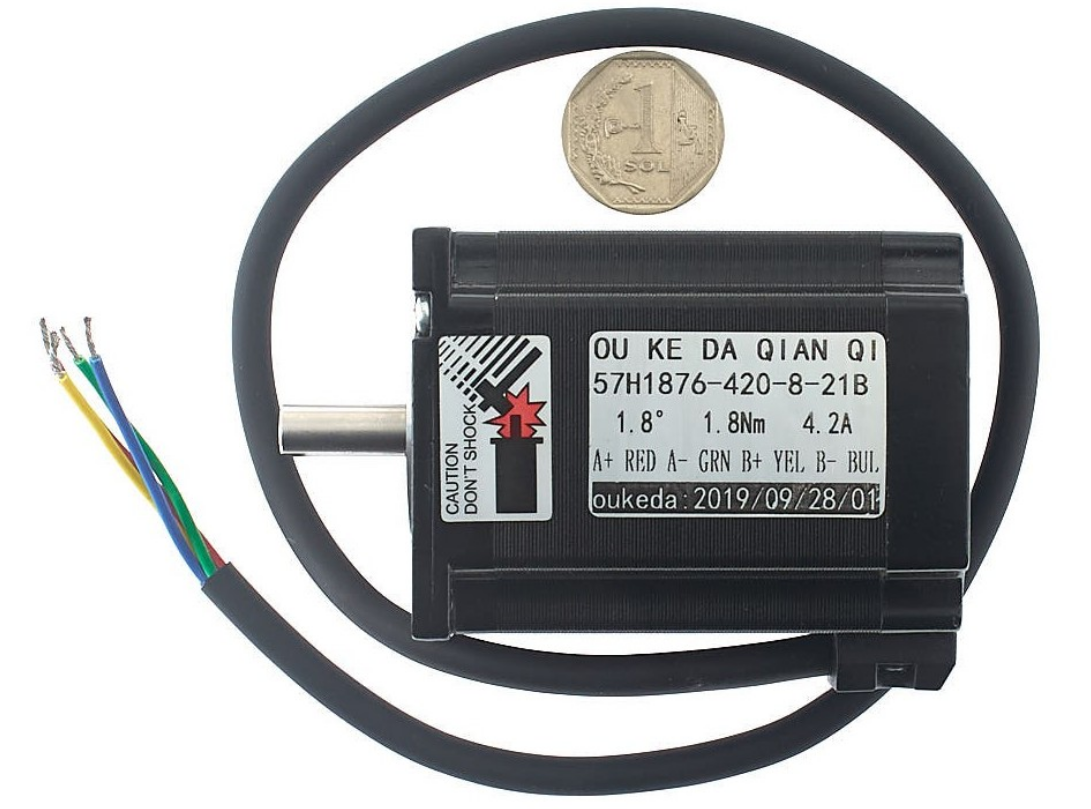
\includegraphics[width=0.92\linewidth,height=0.62\textheight,keepaspectratio]{./media/image157.png}
\captionof*{figure}{\small\itshape Figura 34. Actuador Motor PaP Stepper Nema 23}
\addcontentsline{lof}{figure}{Figura 34. Actuador Motor PaP Stepper Nema 23}
\label{fig:34}
\end{center}

\begin{center}
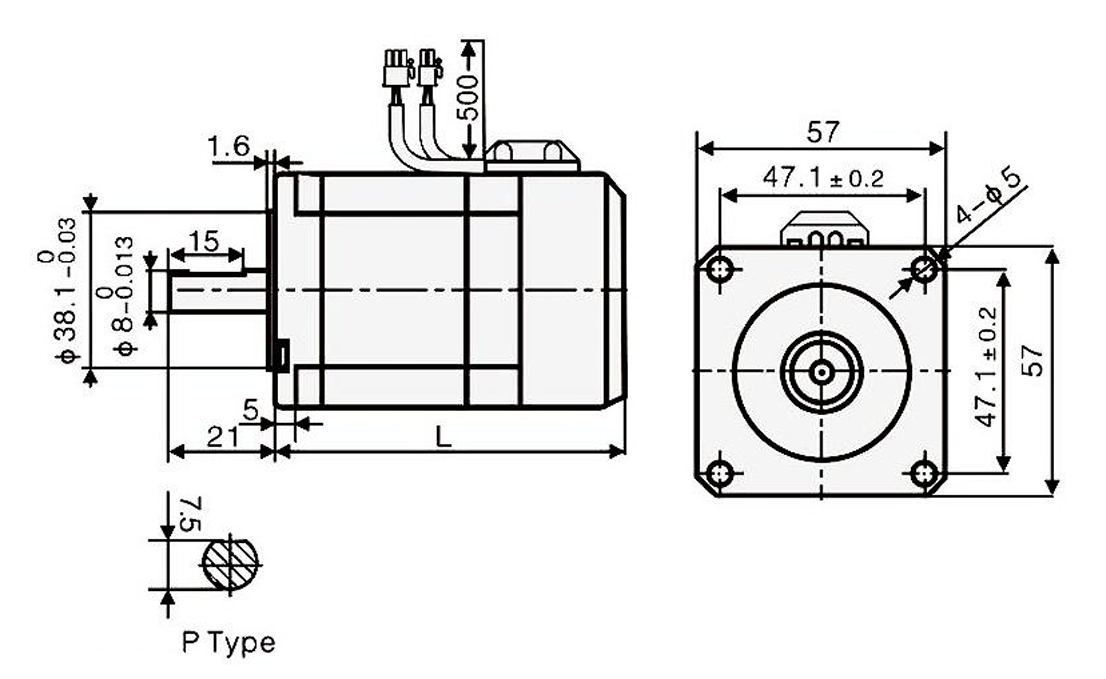
\includegraphics[width=0.92\linewidth,height=0.62\textheight,keepaspectratio]{./media/image88.png}
\captionof*{figure}{\small\itshape Figura 35. Dimensionamiento del Motor PaP Stepper Nema 23}
\addcontentsline{lof}{figure}{Figura 35. Dimensionamiento del Motor PaP Stepper Nema 23}
\label{fig:35}
\end{center}

\textbf{Justificación de selección del Nema 23}

La decisión de implementar un motor paso a paso Nema 23 en lugar de alternativas como servomotores, motores DC con encoder o actuadores lineales eléctricos se fundamenta en requisitos específicos del sistema de posicionamiento de la cámara. El torque máximo de 18.4 kg·cm (1.8 N·m) proporciona capacidad suficiente para desplazar la cámara domo DS-2CE57H0T-VPITF que pesa aproximadamente 600 gramos, más el soporte de montaje y el sistema de deslizamiento sobre rieles.

\textbf{Justificación teórica:}

\begin{center}
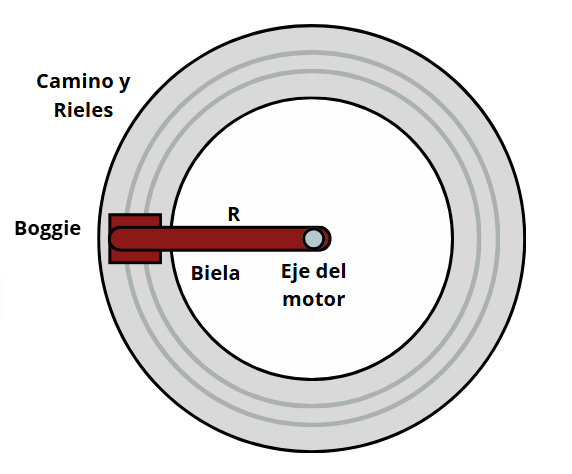
\includegraphics[width=0.92\linewidth,height=0.62\textheight,keepaspectratio]{./media/image139.png}
\captionof*{figure}{\small\itshape Figura 36. Sistema de Movimiento del Boggie de la Cámara\\}
\addcontentsline{lof}{figure}{Figura 36. Sistema de Movimiento del Boggie de la Cámara\\}
\label{fig:36}
\end{center}

En la Figura 36 podemos ver que el Boggie (El cubo) se encuentra sujeto a una Biela que gracias al Motor se realiza el movimiento, vamos a calcular el torque se necesitaría y verificar la elección del Motor Pap 23.\\
\strut \\
El radio desde el eje del motor y el Boggie es de 250 mm. En la Figura 37 vemos más detalles sobre el Boggie y su conexión con la Biela y dimensiones. Cabe mencionar que se calculará el peso con un FS de 2 con el fin de asegurar el motor óptimo, bajo esa premisa el peso establecido sería de 1200 gramos.

\begin{center}
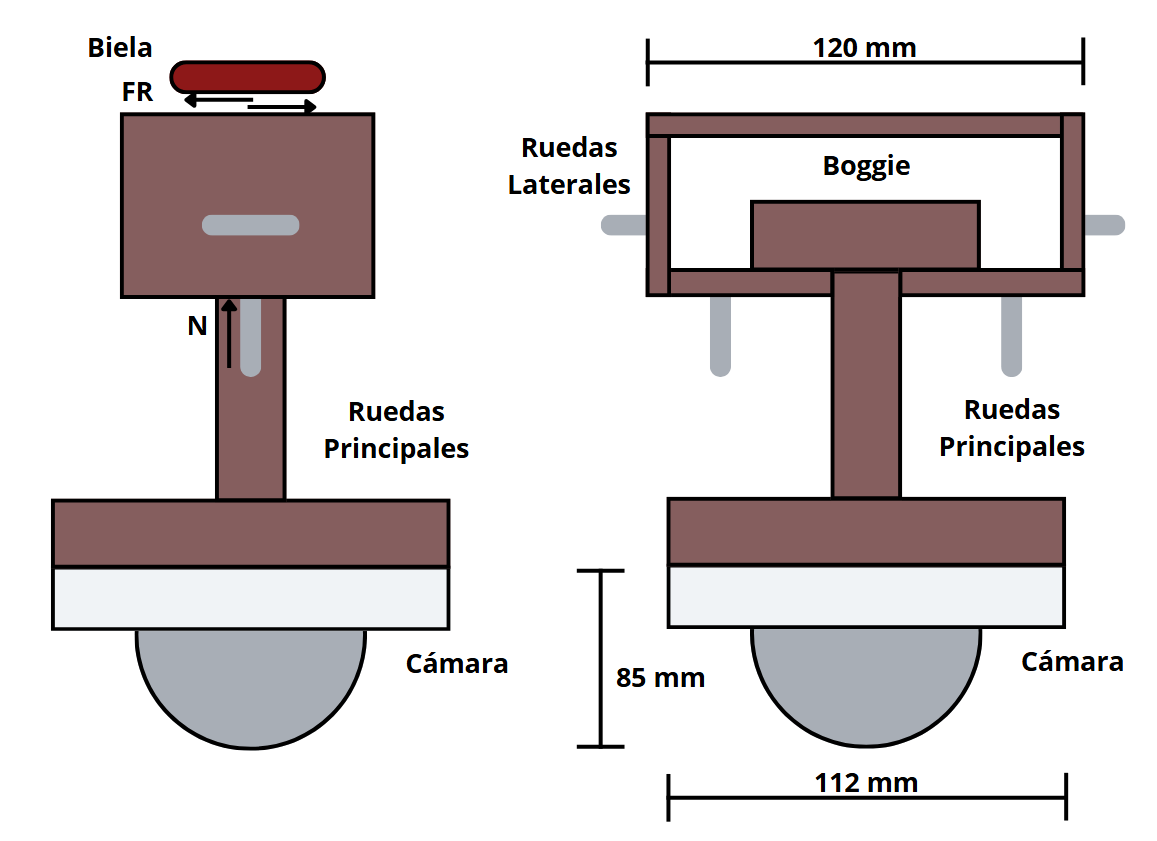
\includegraphics[width=0.92\linewidth,height=0.62\textheight,keepaspectratio]{./media/image54.png}
\captionof*{figure}{\small\itshape Figura 37. Boggie sujeto a la cámara}
\addcontentsline{lof}{figure}{Figura 37. Boggie sujeto a la cámara}
\label{fig:37}
\end{center}

Considerando que los materiales establecidos para la realización tanto de la Biela como del Boggie serán de PLA (Ácido Poliláctico) y elementos de sujeción de acero inoxidable:

\begin{itemize}
\item
  Radio desde el eje del motor al punto de conexión con el boggie: r = 250 mm
\item
  Factor de Seguridad (FS): 2
\item
  Peso de diseño: 1.2 kg (1200 g)
\item
  Coeficiente de Fricción PLA: 0.15
\item
  Aceleración angular de \(2\ rad/s^{2}\)
\end{itemize}

Torque Estático:

\begin{centeredmath}
W\  = \ m\ x\ g\  = \ 1.2\ x\ 9.81\  = \ 11.772\ N
\end{centeredmath}

\begin{centeredmath}
F_{\text{fricción}}\  = \ u\ x\ W\  = \ 0.15\ x\ 11.772\ N\  = \ 1.776
\end{centeredmath}

\begin{centeredmath}
T_{\text{estático}}\  = \ F_{\text{fricción}}\ x\ r\  = \ 1.766\ x\ 0.25m\  = \ 0.441\ N.m
\end{centeredmath}

Torque Dinámico:

\begin{centeredmath}
\alpha_{tangencial\ } = \alpha\ x\ r\  = 2\ rad/s^{2}\ x\ 0.25\  = 0.5\ m/s^{2}
\end{centeredmath}

\begin{centeredmath}
F_{inercia}\  = \ m\ x\ \alpha_{tangencial\ }\  = \ 1.2\ x\ 0.5\  = \ 0.6\ N
\end{centeredmath}

\begin{centeredmath}
T_{\text{dinámico}}\  = \ {(F}_{\text{fricción}}\  + F_{inercia}\ )\ x\ r\  = \ (1.766 + 0.6)\ x\ 0.25m\  = \ 0.591\ N.m
\end{centeredmath}

Fuerzas en la Biela:

\begin{centeredmath}
F_{Biela}\  = \ F_{\text{fricción}} + F_{inercia}\  = \ 1.766 + 0.6\  = \ 2.366\ N
\end{centeredmath}

Sección Transversal de A = \(80\ mm^{2}\)

\begin{centeredmath}
\sigma_{biela} = \ F_{biela}\ /\ A\  = \ 29.58\ KPa
\end{centeredmath}

Dado que la resistencia a tracción del PLA \ensuremath{\approx} 50 MPa, el esfuerzo calculado representa solo el 0.059\% de su límite.

Torque Motor:

\begin{centeredmath}
FS_{MOTOR} = 1.8\ /\ 0.591\  = 3.05
\end{centeredmath}

Dejando un torque disponible de 1.209 N.m con un desplazamiento de:

\begin{centeredmath}
v_{lineal} = w\ x\ r\  = 1.57\ m/s.
\end{centeredmath}

El análisis confirma que el motor paso a paso NEMA 23 seleccionado cumple con los requerimientos del sistema. El torque dinámico requerido (0.591 N·m) representa una tercera parte del torque disponible (1.8 N·m), garantizando un margen de seguridad de 3.05. La velocidad lineal máxima teórica del boggie es de 1.57 m/s, aunque en operación real se trabaja a velocidades menores, lo que permite incrementar el torque efectivo y optimizar el desempeño del sistema.

\textbf{Driver para Motor Stepper}

El control efectivo de un motor paso a paso bipolar requiere un driver dedicado que gestione la conmutación secuencial de corriente en las bobinas del motor con la polaridad y temporización correctas. Para esta aplicación se implementa el driver digital DM542T, dispositivo basado en tecnología DSP (Digital Signal Processor) que genera las secuencias de excitación necesarias y proporciona protecciones eléctricas que salvaguardan tanto el motor como la electrónica de control.

\begin{center}
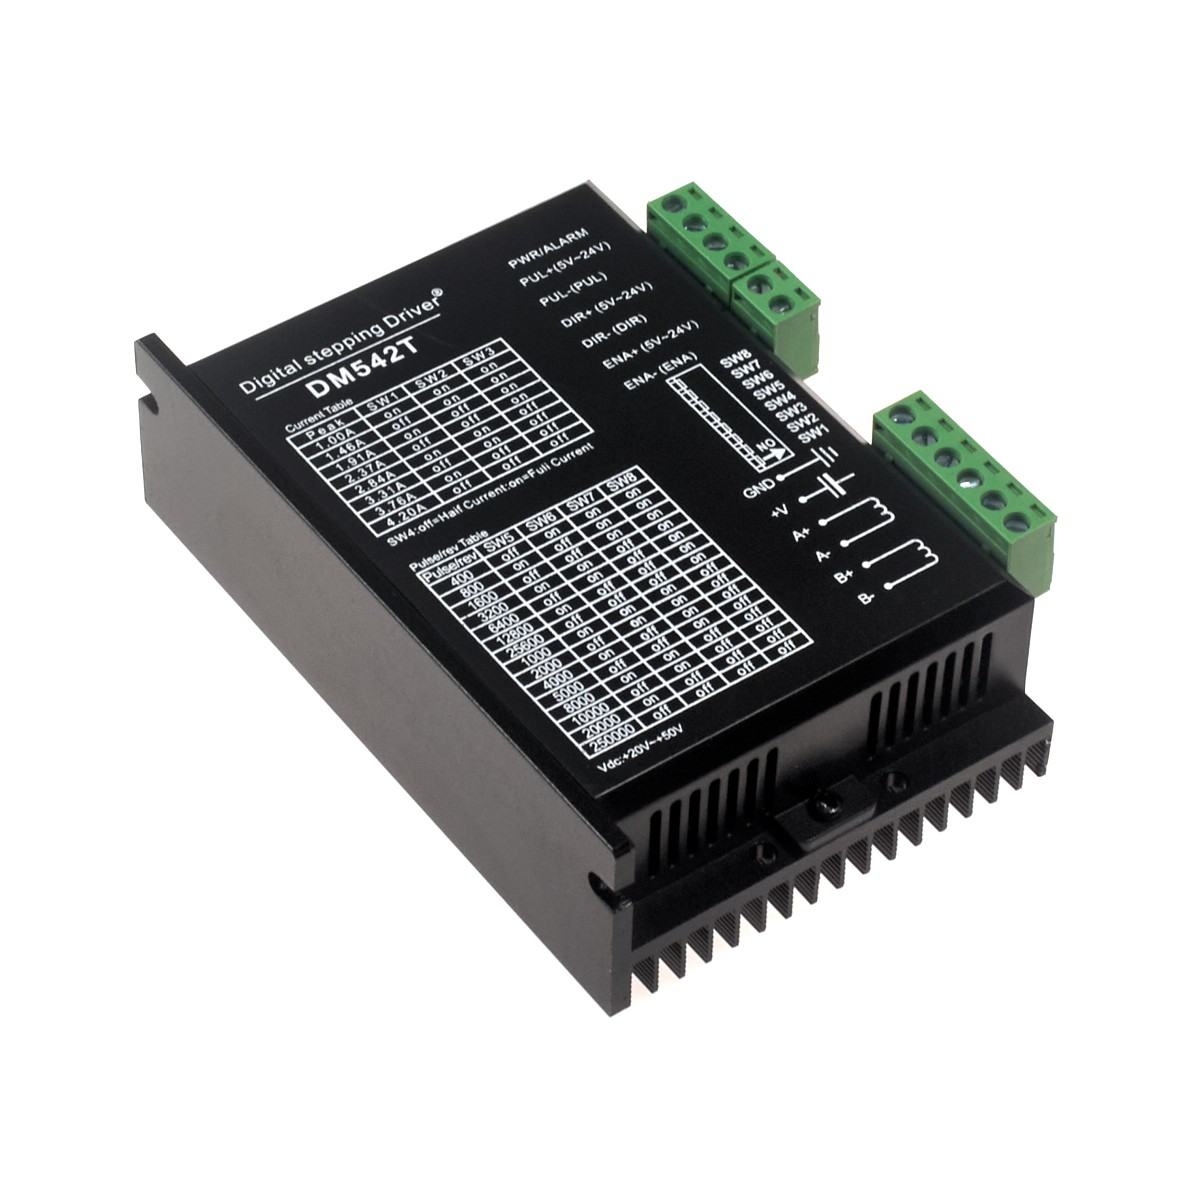
\includegraphics[width=0.92\linewidth,height=0.62\textheight,keepaspectratio]{./media/image153.png}
\captionof*{figure}{\small\itshape Figura 38. Driver DM542T para Motor Stepper}
\addcontentsline{lof}{figure}{Figura 38. Driver DM542T para Motor Stepper}
\label{fig:38}
\end{center}

El driver DM542T emplea control por micropaso, técnica que subdivide cada paso mecánico completo de 1.8 grados en múltiples incrementos menores mediante la modulación simultánea de corriente en ambas fases del motor. Esta capacidad permite seleccionar entre 15 resoluciones diferentes. Para el sistema de cámara semafórica, una configuración típica de 1600 pasos por revolución (micropaso de 1/8) proporciona resolución angular de 0.225 grados, suficiente para posicionar la cámara con precisión en el recorrido lineal sobre los rieles.

El rango de voltaje de alimentación de 18V a 50V DC permite utilizar fuentes de alimentación estándar de 24V o 48V comunes en instalaciones industriales y semafóricas, mientras que el rango de corriente ajustable de 1.0A a 4.5A mediante switches DIP en el dispositivo facilita la configuración precisa para el motor específico seleccionado, que requiere 4.2A nominales por fase. Datos mostrados en la tabla 4.11 de Anexos.

El driver DM542T requiere tres señales digitales de control para operar el motor paso a paso: PUL (pulso), DIR (dirección) y ENA (enable). La señal PUL determina el avance del motor mediante pulsos individuales donde cada transición genera un incremento angular según la configuración de micropaso seleccionada. La señal DIR establece el sentido de rotación (horario o antihorario) dependiendo de su nivel lógico. La señal ENA activa o desactiva la energización de las bobinas del motor, permitiendo deshabilitar cuando no requiere mantener posición para reducir consumo energético y calentamiento.

\textbf{Convertidor de Nivel Lógico}

Para resolver la incompatibilidad de voltajes entre la Raspberry Pi 5 y el driver DM542T se implementa un convertidor de nivel lógico bidireccional de 8 canales basado en el chip TXS0108E. Este dispositivo emplea tecnología de traducción automática de voltaje que detecta la dirección de la señal y realiza la conversión apropiada sin necesidad de configuración de dirección explícita, simplificando significativamente el diseño del circuito de interfaz.

\begin{center}
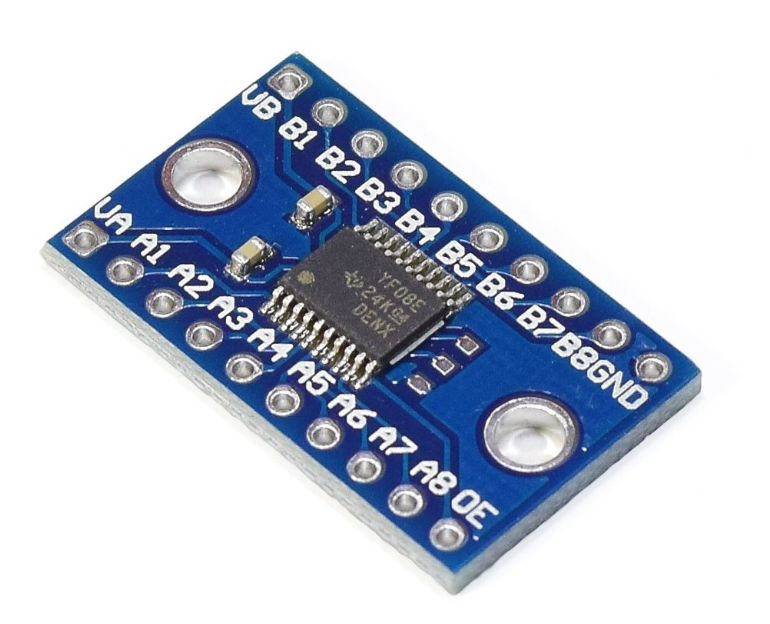
\includegraphics[width=0.92\linewidth,height=0.62\textheight,keepaspectratio]{./media/image20.png}
\captionof*{figure}{\small\itshape Figura 39. Conversor de nivel lógico 8CH 5V/3.3V}
\addcontentsline{lof}{figure}{Figura 39. Conversor de nivel lógico 8CH 5V/3.3V}
\label{fig:39}
\end{center}

La capacidad bidireccional del TXS0108E, aunque no estrictamente necesaria para las señales de control del motor que son unidireccionales desde la Raspberry Pi hacia el driver, proporciona flexibilidad para futuras expansiones del sistema donde podrían requerirse señales de retorno como alarmas o señales de posición límite desde sensores adicionales.

\subsection{Unidades de comunicación con la Nube}\label{unidades-de-comunicaciuxf3n-con-la-nube}

\textbf{4.1.3.1 Módulo 4G LTE HAT con Quectel EG25-G}

La arquitectura del sistema de control adaptativo inteligente para semáforos requiere comunicación bidireccional confiable y de baja latencia con servidores en la nube para transmitir datos de telemetría, recibir comandos de configuración y permitir la coordinación entre múltiples intersecciones. Para esta función crítica se implementa el HAT 4G LTE para Raspberry Pi equipado con el módem celular Quectel EG25-GL, proporcionando conectividad independiente de infraestructura de red fija que podría no estar disponible o ser poco confiable en todas las intersecciones.

El módulo HAT (Hardware Attached on Top) se diseña específicamente para acoplarse sobre la Raspberry Pi utilizando el conector GPIO de 40 pines, estableciendo conexión tanto para alimentación como para comunicación de datos. A diferencia de módulos USB o conexiones por cable que introducen fragilidad mecánica, el formato HAT proporciona acoplamiento mecánico robusto mediante separadores y tornillos que aseguran el módulo firmemente contra vibraciones propias del entorno vial. El diseño incorpora un header de apilamiento (stacking header) que replica todos los pines GPIO en la parte superior del HAT, permitiendo conectar dispositivos adicionales sin perder acceso a los pines que técnicamente ocupa el módulo celular pero que realmente no utiliza en su operación.

\begin{center}
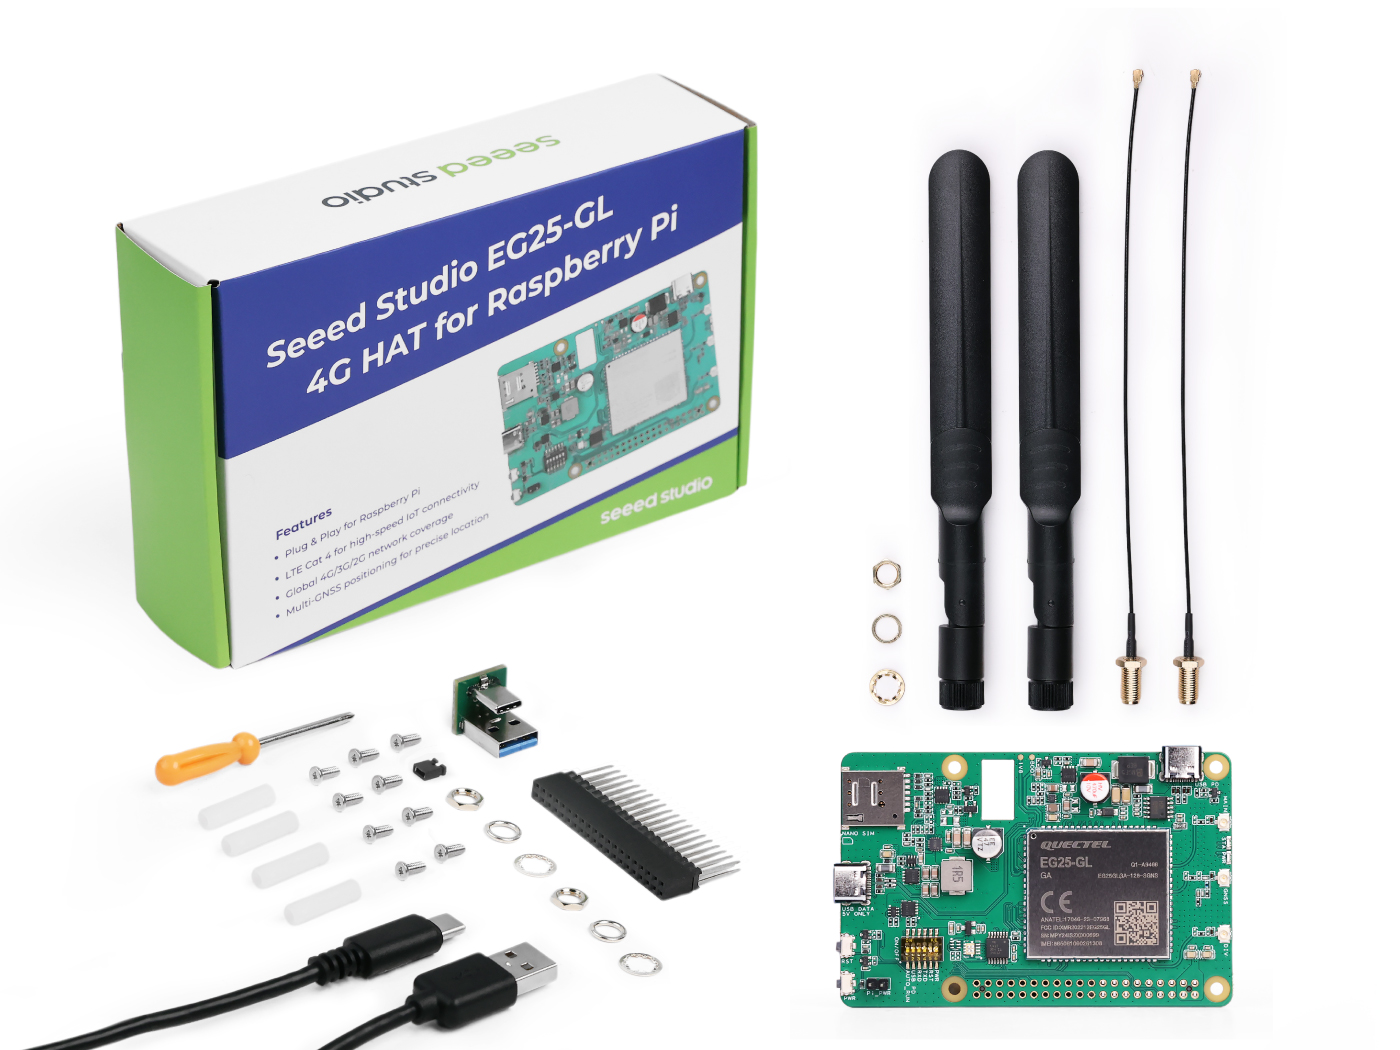
\includegraphics[width=0.92\linewidth,height=0.62\textheight,keepaspectratio]{./media/image68.png}
\captionof*{figure}{\small\itshape Figura 40. HAT 4G LTE para Raspberry Pi}
\addcontentsline{lof}{figure}{Figura 40. HAT 4G LTE para Raspberry Pi}
\label{fig:40}
\end{center}

La decisión de implementar conectividad celular 4G LTE en lugar de alternativas como Wi-Fi, Ethernet o módulos de comunicación por radiofrecuencia propietarios responde a requisitos fundamentales de disponibilidad, cobertura y compatibilidad con infraestructura existente. Las redes celulares 4G proporcionan cobertura virtualmente universal en áreas urbanas donde se encuentran las intersecciones semafóricas, eliminando la dependencia de instalación de cableado Ethernet o puntos de acceso Wi-Fi dedicados que representan costos significativos de infraestructura y mantenimiento. La independencia de redes privadas facilita el despliegue rápido del sistema en nuevas intersecciones sin necesidad de coordinar con proveedores de servicios de internet o gestionar contraseñas y configuraciones de red específicas de cada ubicación.

El módulo Quectel EG25-GL implementa el estándar LTE Category 4, que proporciona velocidades teóricas de hasta 150 Mbps en bajada y 50 Mbps en subida, capacidades que exceden ampliamente los requerimientos de ancho de banda del sistema semafórico. Incluso transmitiendo video comprimido desde la cámara para análisis remoto o depuración, junto con todos los datos de telemetría de sensores y estadísticas de tráfico, el consumo típico de ancho de banda permanece por debajo de 1 Mbps, dejando margen considerable para ráfagas de datos y operación simultánea de múltiples sistemas en la misma celda de red celular.

La compatibilidad multibanda del EG25-GL con prácticamente todas las bandas LTE utilizadas globalmente garantiza operación en diferentes países y con diversos operadores celulares sin necesidad de variantes regionales del hardware. Por último, la capacidad de fallback automático a tecnologías 3G (WCDMA) y 2G (GSM/EDGE) proporciona redundancia de conectividad en áreas con cobertura 4G limitada o durante condiciones de saturación de red, típicas de la ciudad de Lima. Datos en la tabla 4.12 de Anexos.

La arquitectura del HAT 4G LTE integra múltiples subsistemas que expanden las capacidades más allá de la simple conectividad celular. El módem Quectel EG25-GL se comunica con la Raspberry Pi mediante interfaz USB 2.0, apareciendo como un dispositivo de red estándar que el sistema operativo Linux reconoce automáticamente, simplificando significativamente la configuración de software comparado con módulos que requieren drivers propietarios o comandos AT complejos para operación básica.

El subsistema GNSS (Global Navigation Satellite System) integrado proporciona capacidad de geolocalización precisa mediante recepción simultánea de señales GPS (Estados Unidos), GLONASS (Rusia), BeiDou (China), Galileo (Unión Europea) y QZSS (Japón). Esta característica permite al sistema determinar automáticamente su ubicación geográfica durante la instalación, facilitando la configuración inicial y permitiendo verificar que cada unidad semafórica reporta desde la intersección correcta en el sistema de gestión centralizado. La precisión típica de posicionamiento de 2-5 metros resulta suficiente para identificar inequívocamente cada intersección en el sistema.

\textbf{Conectividad Redundante:}

\begin{itemize}
\item
  Comunicación 4G principal para sistemas críticos
\item
  Backup automático a 3G/2G según disponibilidad de red
\item
  GNSS integrado para geolocalización precisa del sistema
\end{itemize}

\textbf{Protocolos de Comunicación Soportados:}

El soporte nativo de múltiples protocolos de comunicación facilita la integración con diferentes arquitecturas de backend en la nube. El protocolo NTCIP (National Transportation Communications for ITS Protocol) sobre TCP/IP resulta particularmente relevante, ya que constituye el estándar internacional para comunicación con sistemas de gestión de tráfico y controladores semafóricos. La implementación de MQTT (Message Queuing Telemetry Transport) proporciona comunicación eficiente tipo publish/subscribe ideal para telemetría IoT, donde múltiples semáforos publican datos a tópicos específicos y se suscriben a comandos de control. Los protocolos HTTP/HTTPS permiten integración con APIs REST y servicios web convencionales, mientras que el soporte SSL/TLS garantiza encriptación de extremo a extremo para proteger la comunicación contra interceptación y manipulación maliciosa.

El rango de temperatura operativa de -35°C a +75°C cubre ampliamente las condiciones ambientales extremas que pueden presentarse en gabinetes semafóricos instalados en exteriores, desde climas árticos hasta ambientes desérticos. El consumo energético reducido de 15.7 mA en modo inactivo minimiza el drenaje de energía cuando no se transmiten datos activamente, aspecto importante en un sistema de operación continua donde la eficiencia energética acumulada representa ahorros significativos y reduce los requerimientos de capacidad del sistema UPS de respaldo.

\subsection{Unidad de control y periféricos}\label{unidad-de-control-y-perifuxe9ricos}

La selección de la unidad de control constituye una decisión crítica en el desarrollo del sistema de control adaptativo inteligente para semáforos, ya que debe integrar capacidades simultáneas de procesamiento de visión por computadora, ejecución de algoritmos de inteligencia artificial, gestión de comunicación IoT y control en tiempo real de dispositivos electromecánicos. Esta sección analiza y justifica la selección del Raspberry Pi 5 de 16 GB como unidad de control principal, junto con los aceleradores de inteligencia artificial y periféricos complementarios necesarios para alcanzar el rendimiento requerido por el sistema.

El proceso de selección de la unidad de control se fundamentó en criterios técnicos específicos que garantizan el rendimiento, escalabilidad y confiabilidad del sistema. La capacidad de procesamiento debe incluir CPU multinúcleo de alto rendimiento capaz de ejecutar sistemas operativos completos y múltiples procesos concurrentes, junto con GPU suficientemente potente para acelerar operaciones de visión por computadora y preprocesamiento de imágenes. La memoria RAM debe proporcionar espacio suficiente para cargar modelos en memoria, mantener buffers de video, ejecutar el sistema operativo y aplicaciones auxiliares sin recurrir a memoria de intercambio en disco que degradaría severamente el rendimiento.

La conectividad representa otro aspecto fundamental, requiriendo múltiples puertos USB para cámara, módulos de comunicación y dispositivos de almacenamiento, puertos GPIO para control de sensores y actuadores, interfaces de red Ethernet y Wi-Fi para conectividad redundante, y capacidad de expansión mediante buses estándar para integrar aceleradores especializados. En este caso comparamos dos unidades de control ampliamente debatidas en la tabla 4.13.

\Needspace{6\baselineskip}
\captionof*{table}{\small\bfseries Tabla 4.13. Comparación técnica de unidades de control evaluadas}
\addcontentsline{lot}{table}{Tabla 4.13. Comparación técnica de unidades de control evaluadas}
\label{tbl:4.13}

\begin{longtable}[]{@{}
  >{\raggedright\arraybackslash}p{(\columnwidth - 4\tabcolsep) * \real{0.2737}}
  >{\raggedright\arraybackslash}p{(\columnwidth - 4\tabcolsep) * \real{0.3579}}
  >{\raggedright\arraybackslash}p{(\columnwidth - 4\tabcolsep) * \real{0.3684}}@{}}
\toprule
\begin{minipage}[b]{\linewidth}\raggedright
Característica
\end{minipage} & \begin{minipage}[b]{\linewidth}\raggedright
Raspberry Pi 5 (16GB)
\end{minipage} & \begin{minipage}[b]{\linewidth}\raggedright
NVIDIA Jetson Nano
\end{minipage} \\
\begin{minipage}[b]{\linewidth}\raggedright
CPU
\end{minipage} & \begin{minipage}[b]{\linewidth}\raggedright
BCM2712 Cortex-A76 4-core @ 2.4GHz
\end{minipage} & \begin{minipage}[b]{\linewidth}\raggedright
Cortex-A57 4-core @ 1.43GHz
\end{minipage} \\
\begin{minipage}[b]{\linewidth}\raggedright
RAM
\end{minipage} & \begin{minipage}[b]{\linewidth}\raggedright
16GB LPDDR4X-4267
\end{minipage} & \begin{minipage}[b]{\linewidth}\raggedright
4GB LPDDR4
\end{minipage} \\
\begin{minipage}[b]{\linewidth}\raggedright
GPU
\end{minipage} & \begin{minipage}[b]{\linewidth}\raggedright
VideoCore VII @ 800MHz
\end{minipage} & \begin{minipage}[b]{\linewidth}\raggedright
128-core Maxwell
\end{minipage} \\
\begin{minipage}[b]{\linewidth}\raggedright
Aceleración IA
\end{minipage} & \begin{minipage}[b]{\linewidth}\raggedright
Coral TPU (4 TOPS)
\end{minipage} & \begin{minipage}[b]{\linewidth}\raggedright
GPU CUDA (472 GFLOPS)
\end{minipage} \\
\begin{minipage}[b]{\linewidth}\raggedright
Interfaces Cámara
\end{minipage} & \begin{minipage}[b]{\linewidth}\raggedright
2x MIPI CSI (4-lane)
\end{minipage} & \begin{minipage}[b]{\linewidth}\raggedright
1x MIPI CSI
\end{minipage} \\
\begin{minipage}[b]{\linewidth}\raggedright
USB
\end{minipage} & \begin{minipage}[b]{\linewidth}\raggedright
2x USB 3.0 + 2x USB 2.0
\end{minipage} & \begin{minipage}[b]{\linewidth}\raggedright
4x USB 3.0
\end{minipage} \\
\begin{minipage}[b]{\linewidth}\raggedright
Ethernet
\end{minipage} & \begin{minipage}[b]{\linewidth}\raggedright
Gigabit + PoE+
\end{minipage} & \begin{minipage}[b]{\linewidth}\raggedright
Gigabit
\end{minipage} \\
\begin{minipage}[b]{\linewidth}\raggedright
Wi-Fi
\end{minipage} & \begin{minipage}[b]{\linewidth}\raggedright
802.11ac dual-band
\end{minipage} & \begin{minipage}[b]{\linewidth}\raggedright
802.11ac
\end{minipage} \\
\begin{minipage}[b]{\linewidth}\raggedright
GPIO
\end{minipage} & \begin{minipage}[b]{\linewidth}\raggedright
40 pines
\end{minipage} & \begin{minipage}[b]{\linewidth}\raggedright
40 pines
\end{minipage} \\
\begin{minipage}[b]{\linewidth}\raggedright
Alimentación
\end{minipage} & \begin{minipage}[b]{\linewidth}\raggedright
5V/5A (25W)
\end{minipage} & \begin{minipage}[b]{\linewidth}\raggedright
5V/4A (20W)
\end{minipage} \\
\midrule
\endhead
\bottomrule
\endlastfoot
\end{longtable}

El análisis comparativo entre Raspberry Pi 5 y NVIDIA Jetson Nano revela ventajas significativas del primero en aspectos críticos para la aplicación semafórica. La CPU Cortex-A76 del Raspberry Pi 5 operando a 2.4 GHz proporciona rendimiento por núcleo aproximadamente 75\% superior a la Cortex-A57 del Jetson Nano a 1.43 GHz, diferencia que se manifiesta directamente en la velocidad de ejecución de código Python para procesamiento de datos de sensores, algoritmos de control adaptativos y gestión de comunicaciones.

La disponibilidad de 16GB de RAM en el Raspberry Pi 5 contrasta dramáticamente con los 4GB del Jetson Nano, diferencia que resulta crucial para aplicaciones de visión por computadora donde los modelos pueden requerir varios gigabytes de memoria solo para los parámetros del modelo. La capacidad de mantener múltiples modelos en memoria simultáneamente (por ejemplo, un modelo principal de detección de vehículos y modelos secundarios para clasificación de tipos vehiculares o detección de peatones) proporciona flexibilidad operativa imposible en sistemas con memoria limitada. Adicionalmente, los buffers de video para procesamiento temporal, las estructuras de datos para seguimiento de objetos entre fotogramas y el sistema operativo con servicios auxiliares consumen memoria significativa que rápidamente satura los 4GB del Jetson Nano.

El puerto PCIe 2.0 x1 del Raspberry Pi 5 representa una ventaja frente al Jetson Nano. Este bus de expansión permite integrar aceleradores de inteligencia artificial externos como el Google Coral TPU mediante adaptadores PCIe, proporcionando capacidad de actualización y escalabilidad imposible en plataformas sin expansión. Aunque el Jetson Nano incluye GPU Maxwell con capacidades CUDA útiles para inteligencia artificial, el ecosistema de modelos optimizados para la arquitectura Coral TPU (basados en TensorFlow Lite) resulta más maduro y accesible.

La disponibilidad de dos interfaces MIPI CSI de 4 carriles en el Raspberry Pi 5 permite conectar dos cámaras simultáneamente sin depender de conversores USB que introducen latencia y consumen ancho de banda. Esta característica habilita configuraciones futuras con visión estereoscópica para estimación de distancias o redundancia de cámaras sin requerir cambio de hardware. El Jetson Nano, con una sola interfaz CSI, limita las opciones de expansión en este aspecto crítico para sistemas de visión. A pesar de que el Raspberry Pi 5 incluye dos interfaces MIPI CSI que permiten conexión directa de cámaras, el sistema implementa una cámara TVI con conversión a USB por versatilidad en el entorno de implementación. Las cámaras TVI sobre cable coaxial ofrecen capacidad de transmisión de video de alta definición hasta 500 metros sin degradación de señal (frente a los 1-2 metros típicos de cables CSI), inmunidad superior a interferencia electromagnética generada por cables de alimentación de alta tensión presentes en postes semafóricos. Las cámaras CSI, aunque ofrecen integración directa, están diseñadas para conexiones cortas dentro de gabinetes electrónicos controlados, no para tendidos exteriores expuestos a condiciones ambientales adversas. La disponibilidad de las interfaces CSI permanece como opción de expansión futura para cámaras secundarias de corto alcance montadas directamente en el gabinete de control.

\textbf{Periféricos y Aceleradores:}

\textbf{Google Coral USB Accelerator}

Para maximizar el rendimiento de inferencia de los modelos utilizados en detección y clasificación vehicular, el sistema integra el acelerador Google Coral USB basado en la Edge TPU (Tensor Processing Unit) de Google. Este dispositivo contiene un procesador especializado diseñado específicamente para ejecutar redes neuronales cuantizadas de manera extremadamente eficiente, liberando la CPU principal de la Raspberry Pi para otras tareas del sistema.

\textbf{Especificaciones técnicas:}

\textbf{Procesador}: Google Edge TPU (Tensor Processing Unit)

\textbf{Rendimiento}: 4 TOPS (Tera Operations Per Second)

\textbf{Consumo}: 2-3 W

\textbf{Interfaz}: USB 3.0 (compatible con Pi 5)

\textbf{Framework}: TensorFlow Lite optimizado

\begin{center}
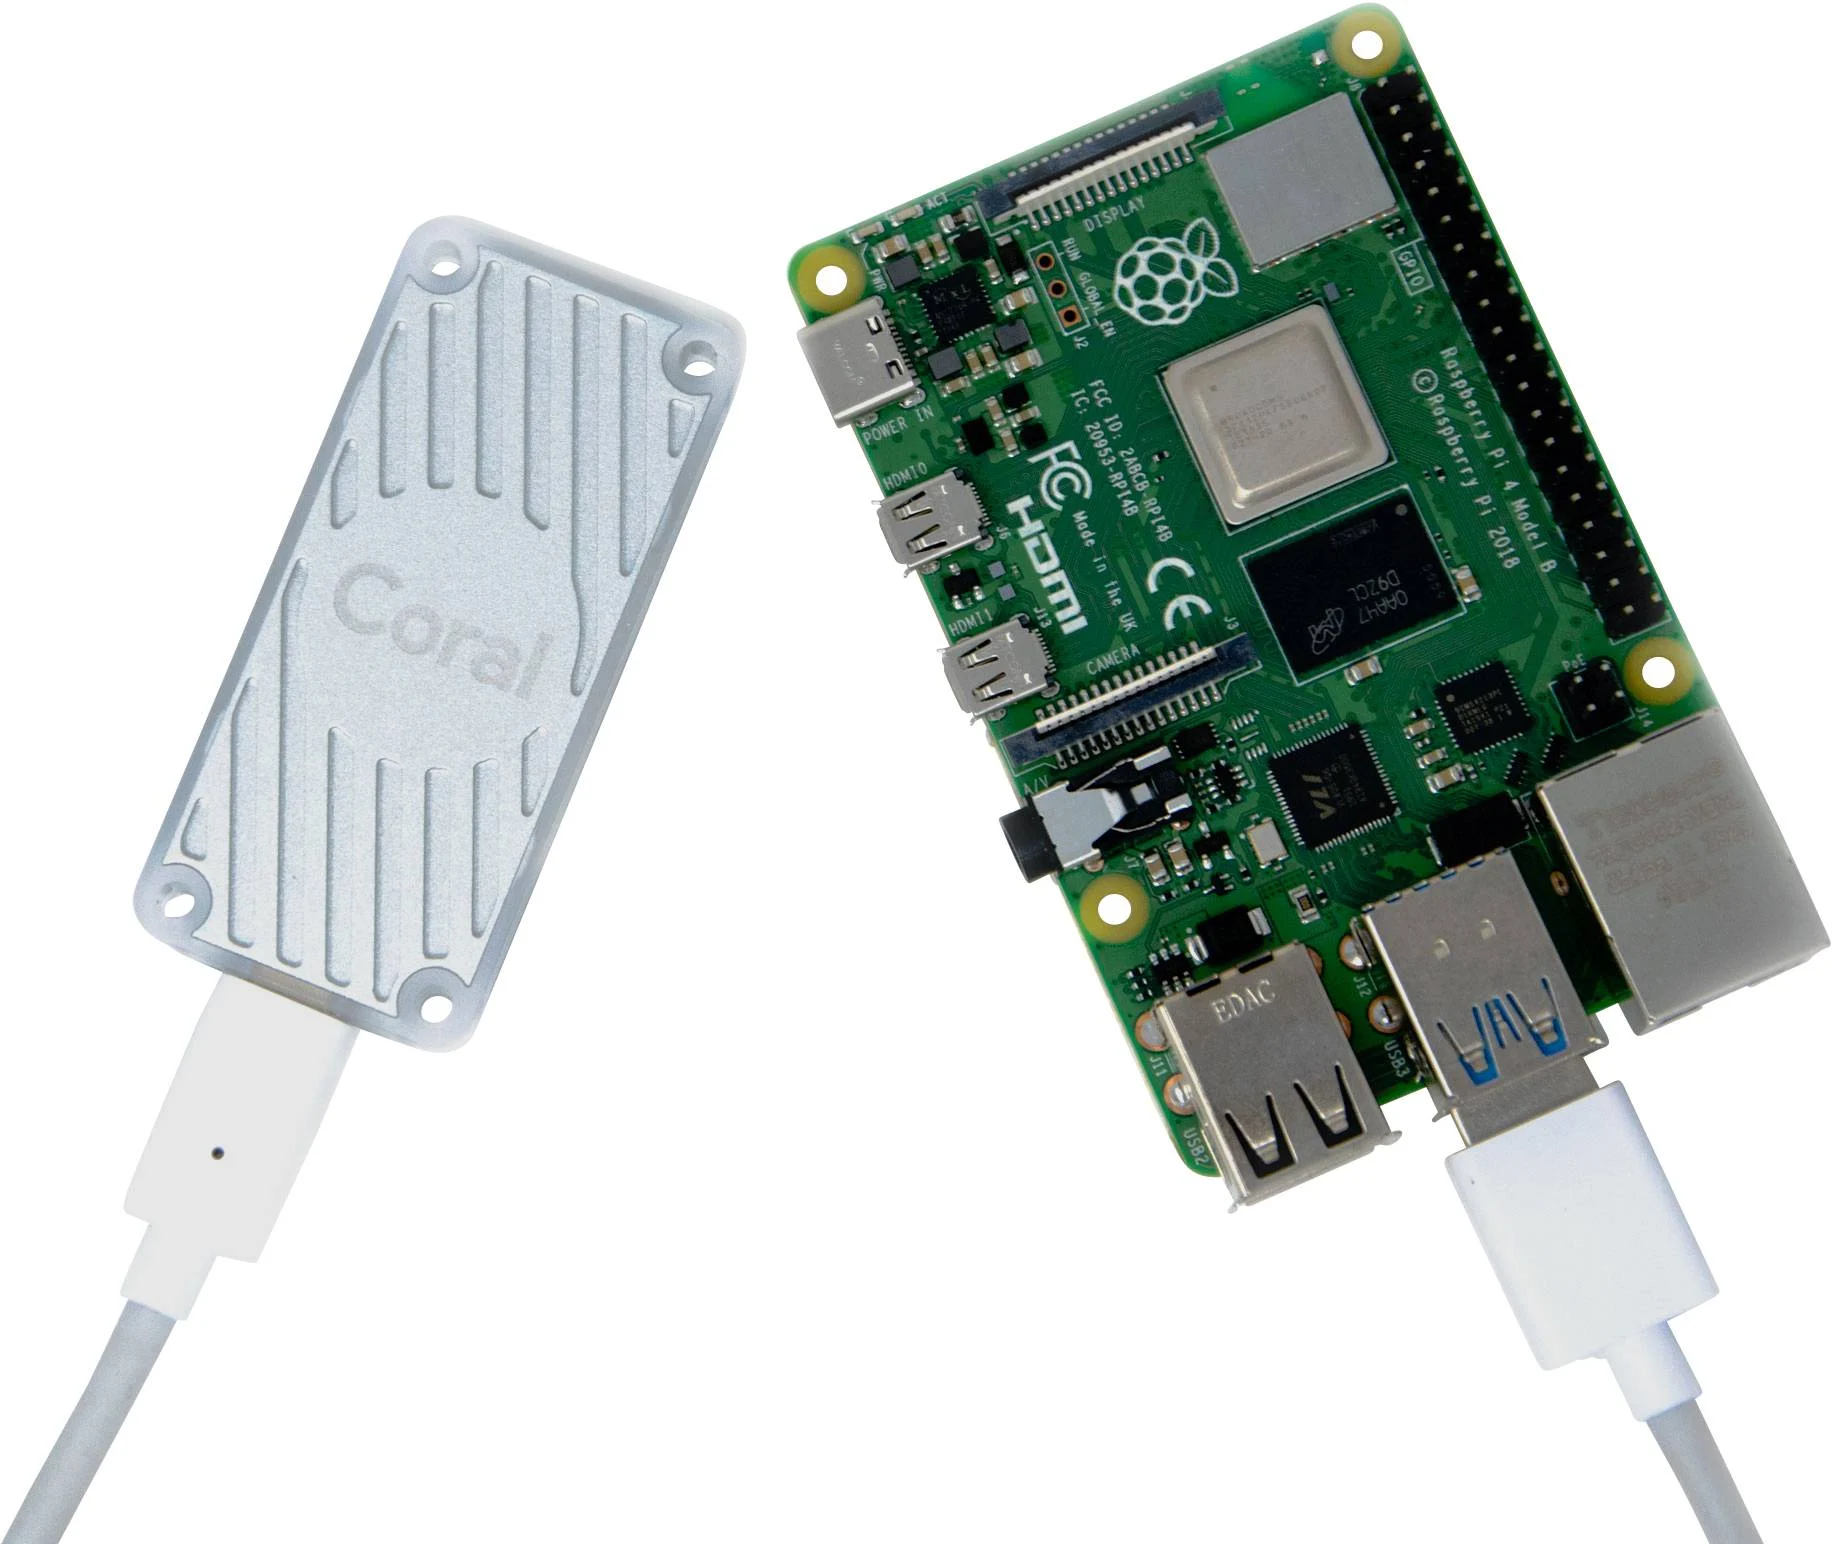
\includegraphics[width=0.92\linewidth,height=0.62\textheight,keepaspectratio]{./media/image21.png}
\captionof*{figure}{\small\itshape Figura 41. Conexión del Raspberry Pi 5 con Google Edge TPU}
\addcontentsline{lof}{figure}{Figura 41. Conexión del Raspberry Pi 5 con Google Edge TPU}
\label{fig:41}
\end{center}

El Google Coral USB Accelerator implementa arquitectura de hardware optimizada para operaciones de multiplicación y acumulación de matrices (MAC), que constituyen la operación fundamental en todas las capas de redes neuronales convolucionales. La Edge TPU alcanza rendimiento de 4 TOPS (Tera Operations Per Second) operando con modelos cuantizados de 8 bits, donde los pesos y activaciones de la red neuronal se representan con enteros de 8 bits en lugar de números de punto flotante de 32 bits. Esta cuantización reduce el tamaño del modelo aproximadamente 4 veces y acelera significativamente las operaciones sin degradación. El rendimiento mejora notablemente en tareas demandantes para la Raspberry Pi.

\subsubsection{\texorpdfstring{4.1.5 Cálculo de consumo energético y selección }{4.1.5 Cálculo de consumo energético y selección }}\label{cuxe1lculo-de-consumo-energuxe9tico-y-selecciuxf3n}

Para garantizar un dimensionamiento adecuado y una operación estable del sistema de control adaptativo inteligente, se realiza un análisis del consumo energético de cada componente. Este análisis se basa en las especificaciones técnicas de los fabricantes, considerando escenarios de carga máxima. El cálculo se estructura en etapas: identificación del consumo por componente, agregación por niveles de voltaje, aplicación de factores de seguridad, selección de fuentes de alimentación y protecciones, y finalmente la elección del UPS con estimación de autonomía. A continuación en la Tabla 4.14 se presenta el Consumo energético de los componentes a utilizar y en la Tabla 4.15 el consumo por voltaje.

\Needspace{6\baselineskip}
\captionof*{table}{\small\bfseries Tabla 4.14. Consumo energético por componente}
\addcontentsline{lot}{table}{Tabla 4.14. Consumo energético por componente}
\label{tbl:4.14}

\begin{longtable}[]{@{}
  >{\raggedright\arraybackslash}p{(\columnwidth - 8\tabcolsep) * \real{0.2594}}
  >{\raggedright\arraybackslash}p{(\columnwidth - 8\tabcolsep) * \real{0.1752}}
  >{\raggedright\arraybackslash}p{(\columnwidth - 8\tabcolsep) * \real{0.1261}}
  >{\raggedright\arraybackslash}p{(\columnwidth - 8\tabcolsep) * \real{0.1384}}
  >{\raggedright\arraybackslash}p{(\columnwidth - 8\tabcolsep) * \real{0.3009}}@{}}
\toprule
\begin{minipage}[b]{\linewidth}\raggedright
\textbf{Componente}
\end{minipage} & \begin{minipage}[b]{\linewidth}\raggedright
\textbf{Voltaje Operación}
\end{minipage} & \begin{minipage}[b]{\linewidth}\raggedright
\textbf{Corriente}
\end{minipage} & \begin{minipage}[b]{\linewidth}\raggedright
\textbf{Potencia (W)}
\end{minipage} & \begin{minipage}[b]{\linewidth}\raggedright
\textbf{Observaciones}
\end{minipage} \\
\begin{minipage}[b]{\linewidth}\raggedright
\textbf{Raspberry Pi 5 (16GB)}
\end{minipage} & \begin{minipage}[b]{\linewidth}\raggedright
5V DC
\end{minipage} & \begin{minipage}[b]{\linewidth}\raggedright
5A
\end{minipage} & \begin{minipage}[b]{\linewidth}\raggedright
25.0
\end{minipage} & \begin{minipage}[b]{\linewidth}\raggedright
Carga máxima con todos los periféricos
\end{minipage} \\
\begin{minipage}[b]{\linewidth}\raggedright
\textbf{Sensor DS18B20}
\end{minipage} & \begin{minipage}[b]{\linewidth}\raggedright
5V DC
\end{minipage} & \begin{minipage}[b]{\linewidth}\raggedright
0.0015A
\end{minipage} & \begin{minipage}[b]{\linewidth}\raggedright
0.0075
\end{minipage} & \begin{minipage}[b]{\linewidth}\raggedright
Corriente durante conversión 1.5mA
\end{minipage} \\
\begin{minipage}[b]{\linewidth}\raggedright
\textbf{Sensor WCS1600}
\end{minipage} & \begin{minipage}[b]{\linewidth}\raggedright
5V DC
\end{minipage} & \begin{minipage}[b]{\linewidth}\raggedright
0.02A
\end{minipage} & \begin{minipage}[b]{\linewidth}\raggedright
0.1
\end{minipage} & \begin{minipage}[b]{\linewidth}\raggedright
Modo normal de operación
\end{minipage} \\
\begin{minipage}[b]{\linewidth}\raggedright
\textbf{Sensor URM06}
\end{minipage} & \begin{minipage}[b]{\linewidth}\raggedright
12V DC
\end{minipage} & \begin{minipage}[b]{\linewidth}\raggedright
0.05A
\end{minipage} & \begin{minipage}[b]{\linewidth}\raggedright
0.6
\end{minipage} & \begin{minipage}[b]{\linewidth}\raggedright
Detección ultrasónica continua
\end{minipage} \\
\begin{minipage}[b]{\linewidth}\raggedright
\textbf{Cámara DS-2CE57H0T-VPITF}
\end{minipage} & \begin{minipage}[b]{\linewidth}\raggedright
12V DC
\end{minipage} & \begin{minipage}[b]{\linewidth}\raggedright
0.5A
\end{minipage} & \begin{minipage}[b]{\linewidth}\raggedright
6.0
\end{minipage} & \begin{minipage}[b]{\linewidth}\raggedright
Con IR encendido (máximo)
\end{minipage} \\
\begin{minipage}[b]{\linewidth}\raggedright
\textbf{Motor Stepper NEMA 23}
\end{minipage} & \begin{minipage}[b]{\linewidth}\raggedright
24V DC
\end{minipage} & \begin{minipage}[b]{\linewidth}\raggedright
4.2A
\end{minipage} & \begin{minipage}[b]{\linewidth}\raggedright
100.8
\end{minipage} & \begin{minipage}[b]{\linewidth}\raggedright
Por fase, operación continua
\end{minipage} \\
\begin{minipage}[b]{\linewidth}\raggedright
\textbf{Driver DM542T}
\end{minipage} & \begin{minipage}[b]{\linewidth}\raggedright
24V DC
\end{minipage} & \begin{minipage}[b]{\linewidth}\raggedright
0.3A
\end{minipage} & \begin{minipage}[b]{\linewidth}\raggedright
7.2
\end{minipage} & \begin{minipage}[b]{\linewidth}\raggedright
Modo standby
\end{minipage} \\
\begin{minipage}[b]{\linewidth}\raggedright
\textbf{HAT 4G LTE (EG25-G)}
\end{minipage} & \begin{minipage}[b]{\linewidth}\raggedright
5V DC
\end{minipage} & \begin{minipage}[b]{\linewidth}\raggedright
0.6A
\end{minipage} & \begin{minipage}[b]{\linewidth}\raggedright
3.0
\end{minipage} & \begin{minipage}[b]{\linewidth}\raggedright
Transmisión activa
\end{minipage} \\
\begin{minipage}[b]{\linewidth}\raggedright
\textbf{Google Coral TPU}
\end{minipage} & \begin{minipage}[b]{\linewidth}\raggedright
5V DC
\end{minipage} & \begin{minipage}[b]{\linewidth}\raggedright
0.6A
\end{minipage} & \begin{minipage}[b]{\linewidth}\raggedright
3.0
\end{minipage} & \begin{minipage}[b]{\linewidth}\raggedright
Inferencia AI activa
\end{minipage} \\
\begin{minipage}[b]{\linewidth}\raggedright
\textbf{Convertidor de Nivel Lógico}
\end{minipage} & \begin{minipage}[b]{\linewidth}\raggedright
5V DC
\end{minipage} & \begin{minipage}[b]{\linewidth}\raggedright
0.01A
\end{minipage} & \begin{minipage}[b]{\linewidth}\raggedright
0.05
\end{minipage} & \begin{minipage}[b]{\linewidth}\raggedright
Bajo consumo
\end{minipage} \\
\begin{minipage}[b]{\linewidth}\raggedright
\textbf{ADC MCP3008}
\end{minipage} & \begin{minipage}[b]{\linewidth}\raggedright
5V DC
\end{minipage} & \begin{minipage}[b]{\linewidth}\raggedright
0.002A
\end{minipage} & \begin{minipage}[b]{\linewidth}\raggedright
0.01
\end{minipage} & \begin{minipage}[b]{\linewidth}\raggedright
Para sensor de corriente
\end{minipage} \\
\midrule
\endhead
\bottomrule
\endlastfoot
\end{longtable}

A continuación, se agrupa el consumo por niveles de voltaje de alimentación para optimizar la distribución de potencia. El cálculo de potencia total por voltaje se realiza sumando los consumos individuales:

\textbf{Consumo por voltajes de alimentación:}

\textbf{5V DC:}

\begin{centeredmath}
25W\  + 3W\  + \ 3W\  + \ 0.05W\  + \ 0.01W\ \  + \ 0.1W + 0.0075W = 31.1675W
\end{centeredmath}

\textbf{12 DC:}

\begin{centeredmath}
6W + 0.6W = 6.6W
\end{centeredmath}

\textbf{24V DC:}

\begin{centeredmath}
100.8W + \ 7.2W = 108W
\end{centeredmath}

\textbf{consumo teórico de diseño:}

\Needspace{6\baselineskip}
\captionof*{table}{\small\bfseries Tabla 4.15. Consumo teórico por voltaje}
\addcontentsline{lot}{table}{Tabla 4.15. Consumo teórico por voltaje}
\label{tbl:4.15}

\begin{longtable}[]{@{}
  >{\raggedright\arraybackslash}p{(\columnwidth - 6\tabcolsep) * \real{0.1688}}
  >{\raggedright\arraybackslash}p{(\columnwidth - 6\tabcolsep) * \real{0.2402}}
  >{\raggedright\arraybackslash}p{(\columnwidth - 6\tabcolsep) * \real{0.2494}}
  >{\raggedright\arraybackslash}p{(\columnwidth - 6\tabcolsep) * \real{0.3415}}@{}}
\toprule
\begin{minipage}[b]{\linewidth}\raggedright
\textbf{Voltaje}
\end{minipage} & \begin{minipage}[b]{\linewidth}\raggedright
\textbf{Potencia (W)}
\end{minipage} & \begin{minipage}[b]{\linewidth}\raggedright
\textbf{Corriente (A)}
\end{minipage} & \begin{minipage}[b]{\linewidth}\raggedright
\textbf{Porcentaje del total}
\end{minipage} \\
\begin{minipage}[b]{\linewidth}\raggedright
\textbf{5V DC}
\end{minipage} & \begin{minipage}[b]{\linewidth}\raggedright
\textbf{31.1675}
\end{minipage} & \begin{minipage}[b]{\linewidth}\raggedright
\textbf{6.23}
\end{minipage} & \begin{minipage}[b]{\linewidth}\raggedright
\textbf{21.4\%}
\end{minipage} \\
\begin{minipage}[b]{\linewidth}\raggedright
\textbf{12V DC}
\end{minipage} & \begin{minipage}[b]{\linewidth}\raggedright
\textbf{6.6}
\end{minipage} & \begin{minipage}[b]{\linewidth}\raggedright
\textbf{0.55}
\end{minipage} & \begin{minipage}[b]{\linewidth}\raggedright
\textbf{4.5\%}
\end{minipage} \\
\begin{minipage}[b]{\linewidth}\raggedright
\textbf{24V DC}
\end{minipage} & \begin{minipage}[b]{\linewidth}\raggedright
\textbf{108.0}
\end{minipage} & \begin{minipage}[b]{\linewidth}\raggedright
\textbf{4.5}
\end{minipage} & \begin{minipage}[b]{\linewidth}\raggedright
\textbf{74.1\%}
\end{minipage} \\
\begin{minipage}[b]{\linewidth}\raggedright
\textbf{TOTAL}
\end{minipage} & \begin{minipage}[b]{\linewidth}\raggedright
\textbf{145.7675 W}
\end{minipage} & \begin{minipage}[b]{\linewidth}\raggedright
\end{minipage} & \begin{minipage}[b]{\linewidth}\raggedright
\textbf{100\%}
\end{minipage} \\
\midrule
\endhead
\bottomrule
\endlastfoot
\end{longtable}

La potencia total del sistema sin factor de seguridad es aproximadamente 146 W, por lo que bajo la norma de Controladores Semafóricos NEMA Standards Publication TS 2-2021 aplicaremos un factor de seguridad del 25\% para garantizar operación estable:

\begin{centeredmath}
145.7675W\ X\ 1.25 = 182.21W
\end{centeredmath}

\textbf{Convertidores DC-DC auxiliares}

Dado que la arquitectura del sistema centraliza la alimentación principal en 24 V DC (debido a su alto porcentaje de consumo del 74.1\%), se derivan los voltajes secundarios (5 V y 12 V) mediante convertidores DC-DC de alta eficiencia. Esto con el fin de minimizar pérdidas en conversión y reduce EMI. Los convertidores se dimensionan considerando que no operan al 100\% de su capacidad para prolongar la vida útil y mejorar la disipación térmica; típicamente, se recomienda operar al 80-90\% de la capacidad nominal para evitar sobrecalentamiento y caídas de eficiencia.

Para 12 V DC: Se selecciona el PULS CD5.121, con potencia máxima de 96 W. La potencia requerida con factor de seguridad se encuentra por debajo del 100\% por una gran diferencia. La eficiencia típica del 88.2\% implica pérdidas bajas. Datos en la tabla 4.16.

\begin{center}
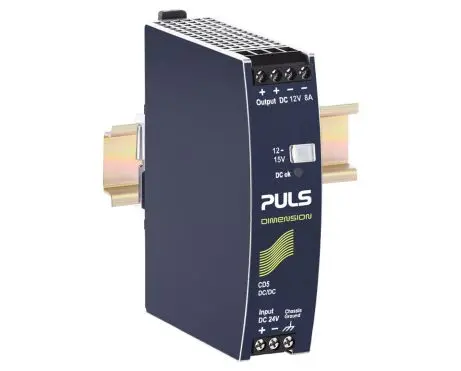
\includegraphics[width=0.92\linewidth,height=0.62\textheight,keepaspectratio]{./media/image86.png}
\captionof*{figure}{\small\itshape Figura 42. Convertidor DC - DC PULS CD5.121}
\addcontentsline{lof}{figure}{Figura 42. Convertidor DC - DC PULS CD5.121}
\label{fig:42}
\end{center}

\textbf{Justificación técnica:\\
} La potencia requerida en la línea de 12 V (6.6 W) representa solo un 6.9 \% de la capacidad nominal del convertidor (96 W). Incluso considerando pérdidas por eficiencia del 88.2 \%, la potencia disponible sería de 84.67 W.

\begin{centeredmath}
Potencia_{Salida\ DC\  - \ 12} = 96\ W\ x\ 0.882\  = \ 84.67\ W
\end{centeredmath}

Esta capacidad es \textbf{suficiente} para alimentar los componentes de 12 V DC, es decir:

\begin{itemize}
\item
  La \textbf{cámara DS-2CE57H0T-VPITF}, con consumo máximo de 6 W.
\item
  El \textbf{sensor ultrasónico URM06}, con consumo promedio de 0.6 W.
\end{itemize}

Ambos dispositivos operarán con amplio margen térmico y sin caídas de tensión, incluso ante picos simultáneos o degradación de eficiencia por temperatura.

Para 5 V DC: Se selecciona el PULS CD5.051 (5 V / 10 A / 50 W). El convertidor CD5.051 es parte de la serie CD de PULS, diseñado para convertir 24 V DC a 5 V DC en un módulo compacto (32 mm de ancho) con reserva de potencia del 20 \% y eficiencia típica alta. Datos en la tabla 4.17.

\begin{center}
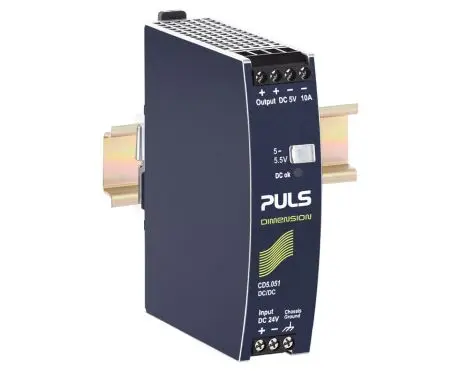
\includegraphics[width=0.92\linewidth,height=0.62\textheight,keepaspectratio]{./media/image87.png}
\captionof*{figure}{\small\itshape Figura 43. Convertidor DC - DC PULS CD5.051}
\addcontentsline{lof}{figure}{Figura 43. Convertidor DC - DC PULS CD5.051}
\label{fig:43}
\end{center}

\textbf{Justificación técnica:}

\begin{centeredmath}
Potencia_{Salida\ DC\  - \ 5} = 50\ W\ x\ 0.815\  = \ 40.75\ W\qquad (1)
\end{centeredmath}

\begin{itemize}
\item
  Demanda: 31.17 W,  6.23 A.
\item
  CD5.051 (potencia útil): 40.75 W,  8.15 A.
\item
  Margen de potencia: 40.75 - 31.17 = 9.58 W \ensuremath{\approx} 30.7 \% de margen sobre la demanda.
\item
  Margen de corriente: 8.15 A - 6.23 A = 1.92 A
\end{itemize}

Por tanto, un CD5.051 cubre holgadamente la carga prevista en 5 V con margen para picos transitorios y expansión ligera.

La potencia total en la entrada de los convertidores DC-DC (desde 24 V) incluye las pérdidas:

\begin{centeredmath}
Potencia_{Entrada\ DC - DC} = P_{5v}\ /\ n_{5v}\  + \ P_{12v}\ /\ n_{12v}\  = \ 56.86\ W\qquad (2)
\end{centeredmath}

Sumado al consumo directo en 24 V la potencia total requerida en 24 V es:

\begin{centeredmath}
P_{24v} = 108\ W\ x\ 1.25\  + 56.86\ W\  = 191.86\ W\qquad (3)
\end{centeredmath}

\textbf{Selección de fuente de alimentación conmutada (SMPS)}

Para alimentar el sistema desde la red AC 220V 60Hz, se selecciona una fuente de alimentación conmutada de 24 VDC de salida. Para alimentar directamente los componentes de alto consumo y los convertidores DC-DC. El modelo debe superar la potencia de diseño ajustada y ofrecer alta eficiencia

El modelo elegido debe superar la potencia de diseño ajustada (191.86 W) y ofrecer alta eficiencia para minimizar pérdidas térmicas y garantizar estabilidad eléctrica.

Se selecciona el modelo S-360-24, con potencia nominal de 360 W, valor que supera la potencia requerida del sistema:

\begin{centeredmath}
Margen = 360\ /\ 191.86\  = 1.88\qquad (1)
\end{centeredmath}

Esto equivale a un 88 \% de margen adicional, lo que brinda escalabilidad y seguridad operativa.

La corriente máxima de salida (15 A) también supera la corriente total requerida en la línea de 24 V:

\begin{centeredmath}
I_{24V\  - \ Total} = 191.86\ /\ 24\  = \ 8A\qquad (2)
\end{centeredmath}

Por lo tanto, la fuente trabaja con amplio margen de corriente disponible, incluso considerando factores de corrección o picos de carga.

Las pérdidas aproximadas de la SMPS (84 \%) necesarias para entregar la potencia de diseño son:

\begin{centeredmath}
P_{\text{pérdidas-SMPS}} = 191.86\ x\ (1 - 0.84)/0.84\  = \ 36.54\ W\qquad (3)
\end{centeredmath}

La SMPS operará a:

\begin{centeredmath}
Carga_{Relativa} = 191.86\ /\ 360\  = 53.3\%\ de\ su\ capacidad\qquad (4)
\end{centeredmath}

\begin{center}
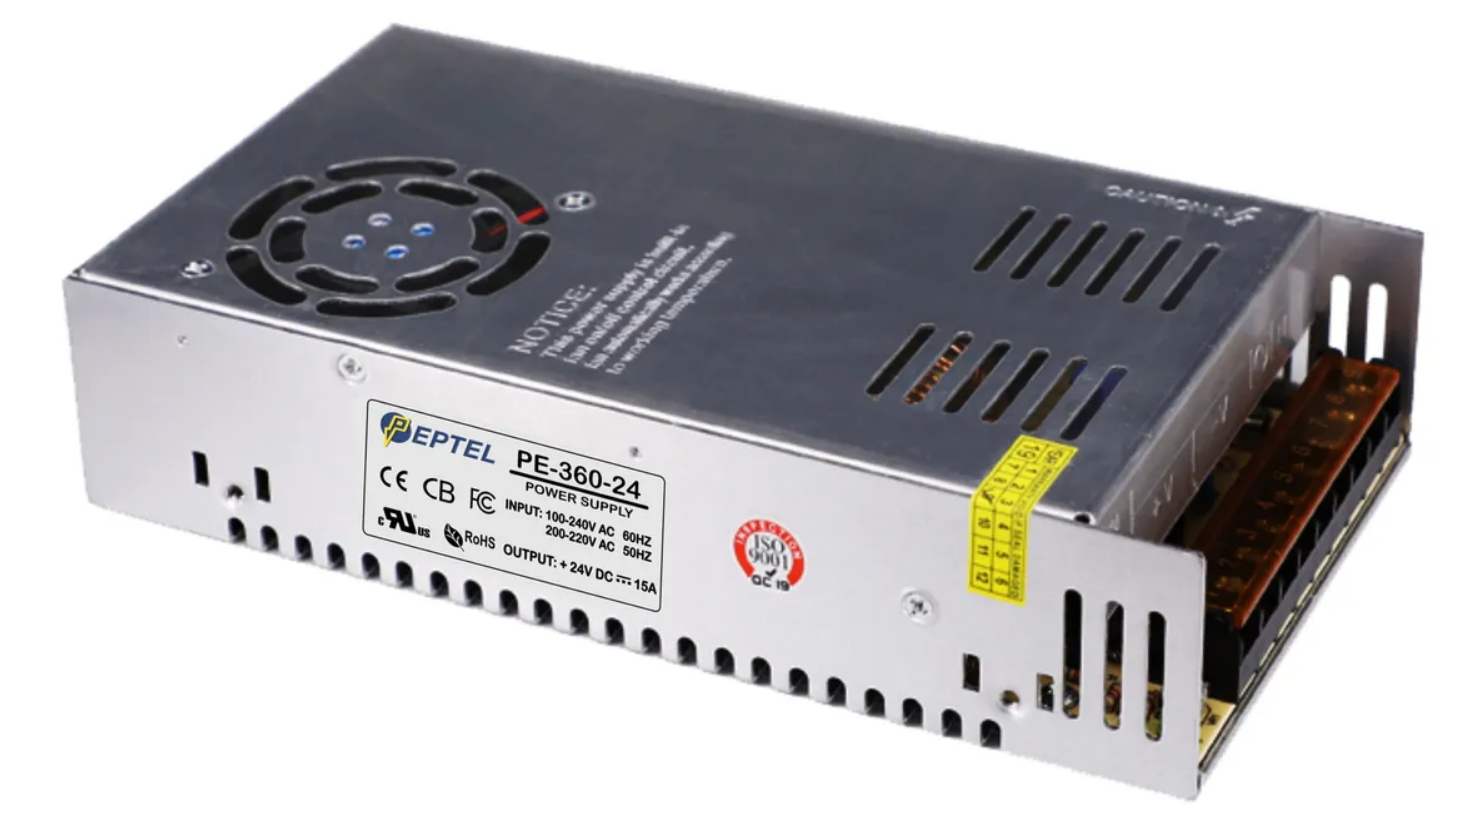
\includegraphics[width=0.92\linewidth,height=0.62\textheight,keepaspectratio]{./media/image114.png}
\captionof*{figure}{\small\itshape Figura 44. Fuente de alimentación conmutada AC/DC 360W 24V 15A}
\addcontentsline{lof}{figure}{Figura 44. Fuente de alimentación conmutada AC/DC 360W 24V 15A}
\label{fig:44}
\end{center}

Los datos se encuentran en la tabla 4.18. Esto la sitúa dentro de la zona óptima de eficiencia, reduciendo el estrés térmico y favoreciendo la vida útil.

\textbf{Cálculo de corriente de entrada desde la red}

\textbf{Corriente AC de entrada:}

Considerando la eficiencia de la fuente (85\%):

\begin{centeredmath}
Potencia_{AC - Entrada} = 191.86\ W\  \div \ 0.85\  = \ 228.4\ W\qquad (1)
\end{centeredmath}

\begin{centeredmath}
Corriente{}_{AC} = 228.4\ W\  \div \ 220V\  = \ 1.04\ A\qquad (2)
\end{centeredmath}

Rango de monitoreo para el sensor de corriente WCS1600: establecer umbrales de alerta del \ensuremath{\pm}20 \% alrededor de 1.04 A \ensuremath{\rightarrow} {[}0.83 A, 1.25 A{]}.

\textbf{Selección del Sistema de Alimentación Ininterrumpida (UPS)\\
}

Para mantener la continuidad durante cortes de energía, se selecciona un UPS upstream de la SMPS, con potencia nominal superior a la requerida y autonomía calculada. Datos mencionados en la tabla 4.19.

\begin{center}
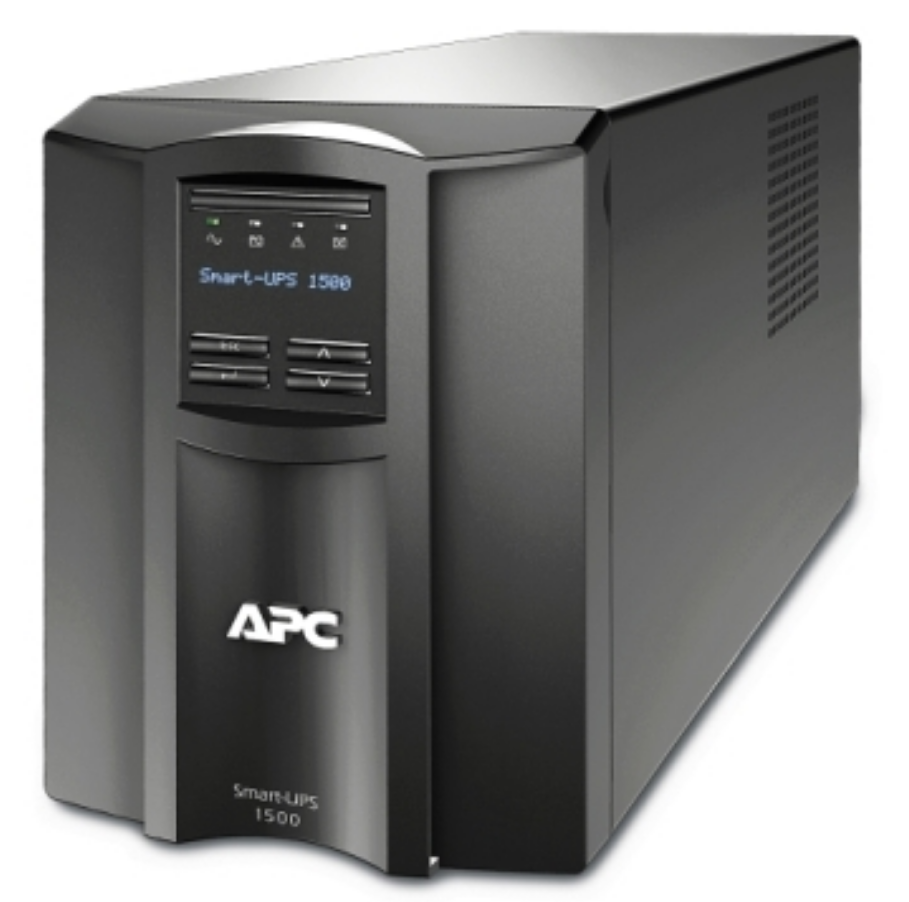
\includegraphics[width=0.92\linewidth,height=0.62\textheight,keepaspectratio]{./media/image6.png}
\captionof*{figure}{\small\itshape Figura 45. UPS}
\addcontentsline{lof}{figure}{Figura 45. UPS}
\label{fig:45}
\end{center}

\textbf{Cálculo de autonomía del UPS:}

\begin{centeredmath}
Capacidad_{\text{batería}} = 2\ x\ 12V\ x\ 12Ah\  = 288\ Wh\qquad (3)
\end{centeredmath}

\begin{centeredmath}
Potencia_{Disponible} = 288\ Wh\ x\ 0.95\  = 273.6\ Wh\qquad (4)
\end{centeredmath}

Calculamos el tiempo de autonomía usando el dato de potencia (1):

\begin{centeredmath}
Tiempo_{\text{autonomía}} = 273.6\ Wh\  \div \ 228.4\ Wh\  = 72\ min\ \qquad (5)
\end{centeredmath}

Margen del UPS (1000 W sobre 228.4 W):

\begin{centeredmath}
Margen = 1000\ /\ 228.4\  = 4.38\qquad (6)
\end{centeredmath}

Esto quiere decir que el UPS nominal puede entregar aproximadamente 4.4 veces la potencia que nuestro sistema demanda en condiciones de diseño. Ese margen facilita expansiones, permite trabajar con menos estrés térmico y mejora la vida útil de las baterías, reduce la probabilidad de activación de protecciones por sobrecarga.

\textbf{Selección de protecciones eléctricas}

\textbf{Interruptor termomagnético (Breaker) - Schneider Electric C60N-C6}

El interruptor termomagnético es un dispositivo de protección que combina dos funciones: protección térmica contra sobrecargas sostenidas mediante un elemento bimetálico, y protección magnética contra cortocircuitos mediante un electroimán. Interrumpe automáticamente el circuito cuando detecta corrientes anormales, protegiendo cables, equipos y previniendo incendios eléctricos. Datos en tabla 4.20.

\begin{center}
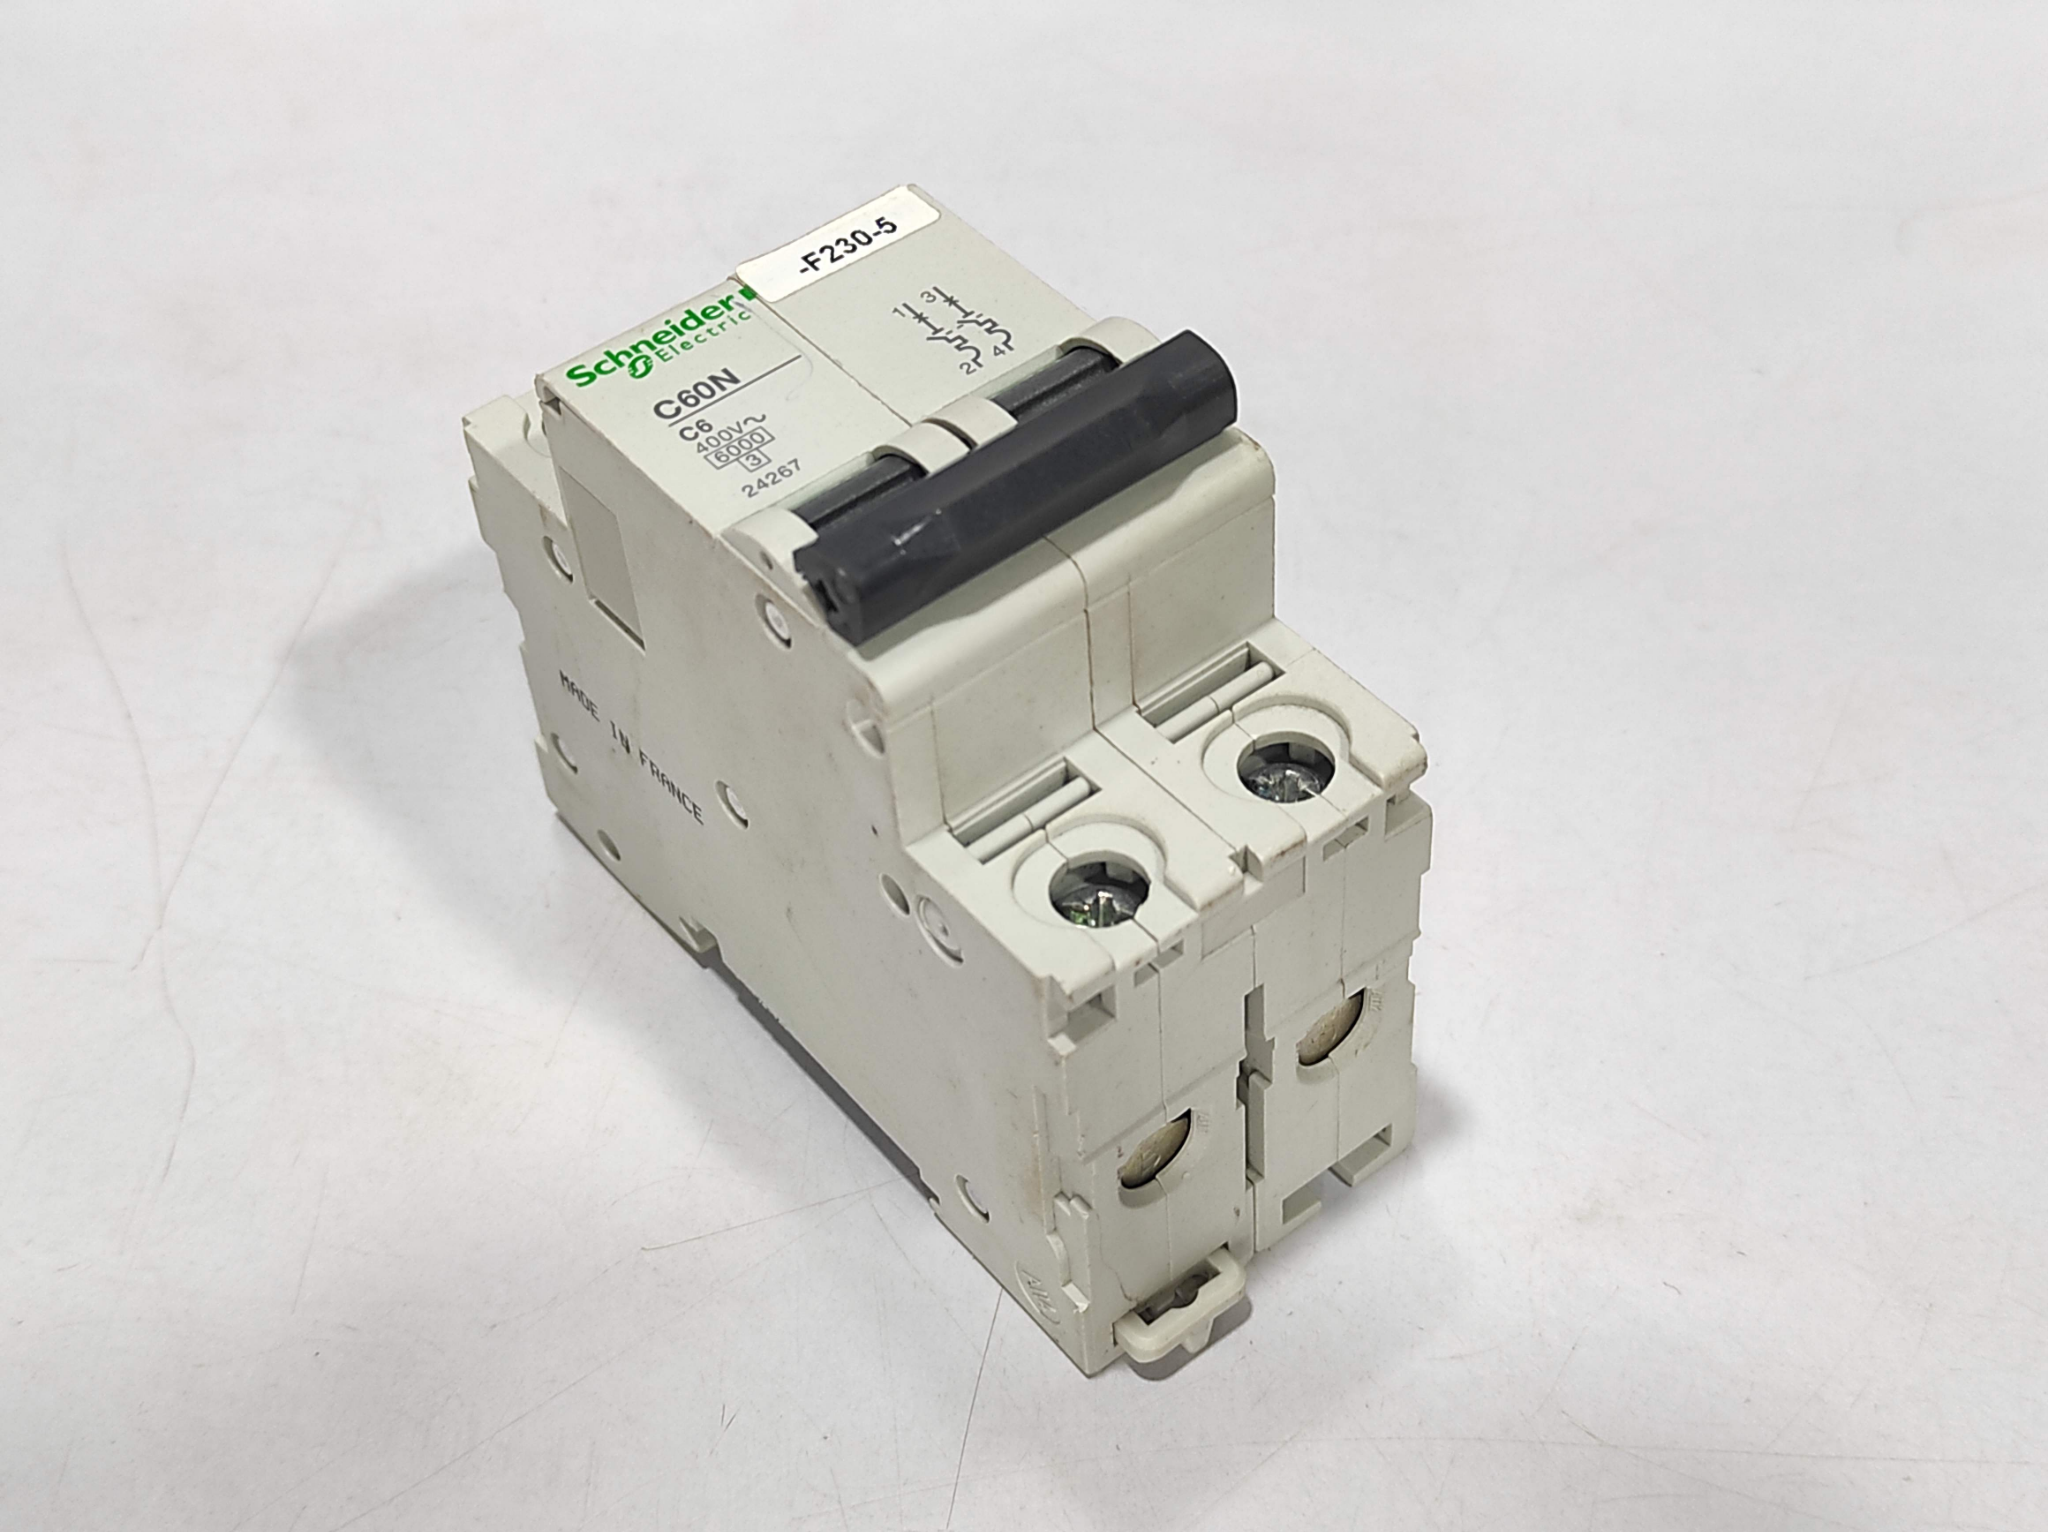
\includegraphics[width=0.92\linewidth,height=0.62\textheight,keepaspectratio]{./media/image72.png}
\captionof*{figure}{\small\itshape Figura 46. Breaker Schneider Electric C60N-C6}
\addcontentsline{lof}{figure}{Figura 46. Breaker Schneider Electric C60N-C6}
\label{fig:46}
\end{center}

Justificación:

La corriente nominal del breaker debe ser superior a la corriente de operación normal, pero lo suficientemente ajustada para proteger adecuadamente. Aplicando el criterio de la NEC (National Electrical Code) y normas IEC:

I\_breaker \ensuremath{\geq} 1.25 \ensuremath{\times} I\_operación\\
I\_breaker \ensuremath{\geq} 1.25 \ensuremath{\times} 1.04 A = 1.3 A

Margen de protección: 6A / 1.04A = 5.77 (factor de seguridad de 5.77)

Curva Tipo C: Diseñada para cargas con componentes electrónicos que generan picos moderados

\textbf{Dispositivo de Protección contra Sobretensiones - Phoenix Contact VAL-MS 230}

El DPS (Dispositivo de Protección contra Sobretensiones) o SPD (Surge Protection Device) es un componente que protege equipos electrónicos sensibles contra sobretensiones transitorias causadas por rayos, conmutación de cargas inductivas o perturbaciones en la red eléctrica. Desvía a tierra las corrientes de sobretensión antes de que alcancen los equipos protegidos.

\begin{center}
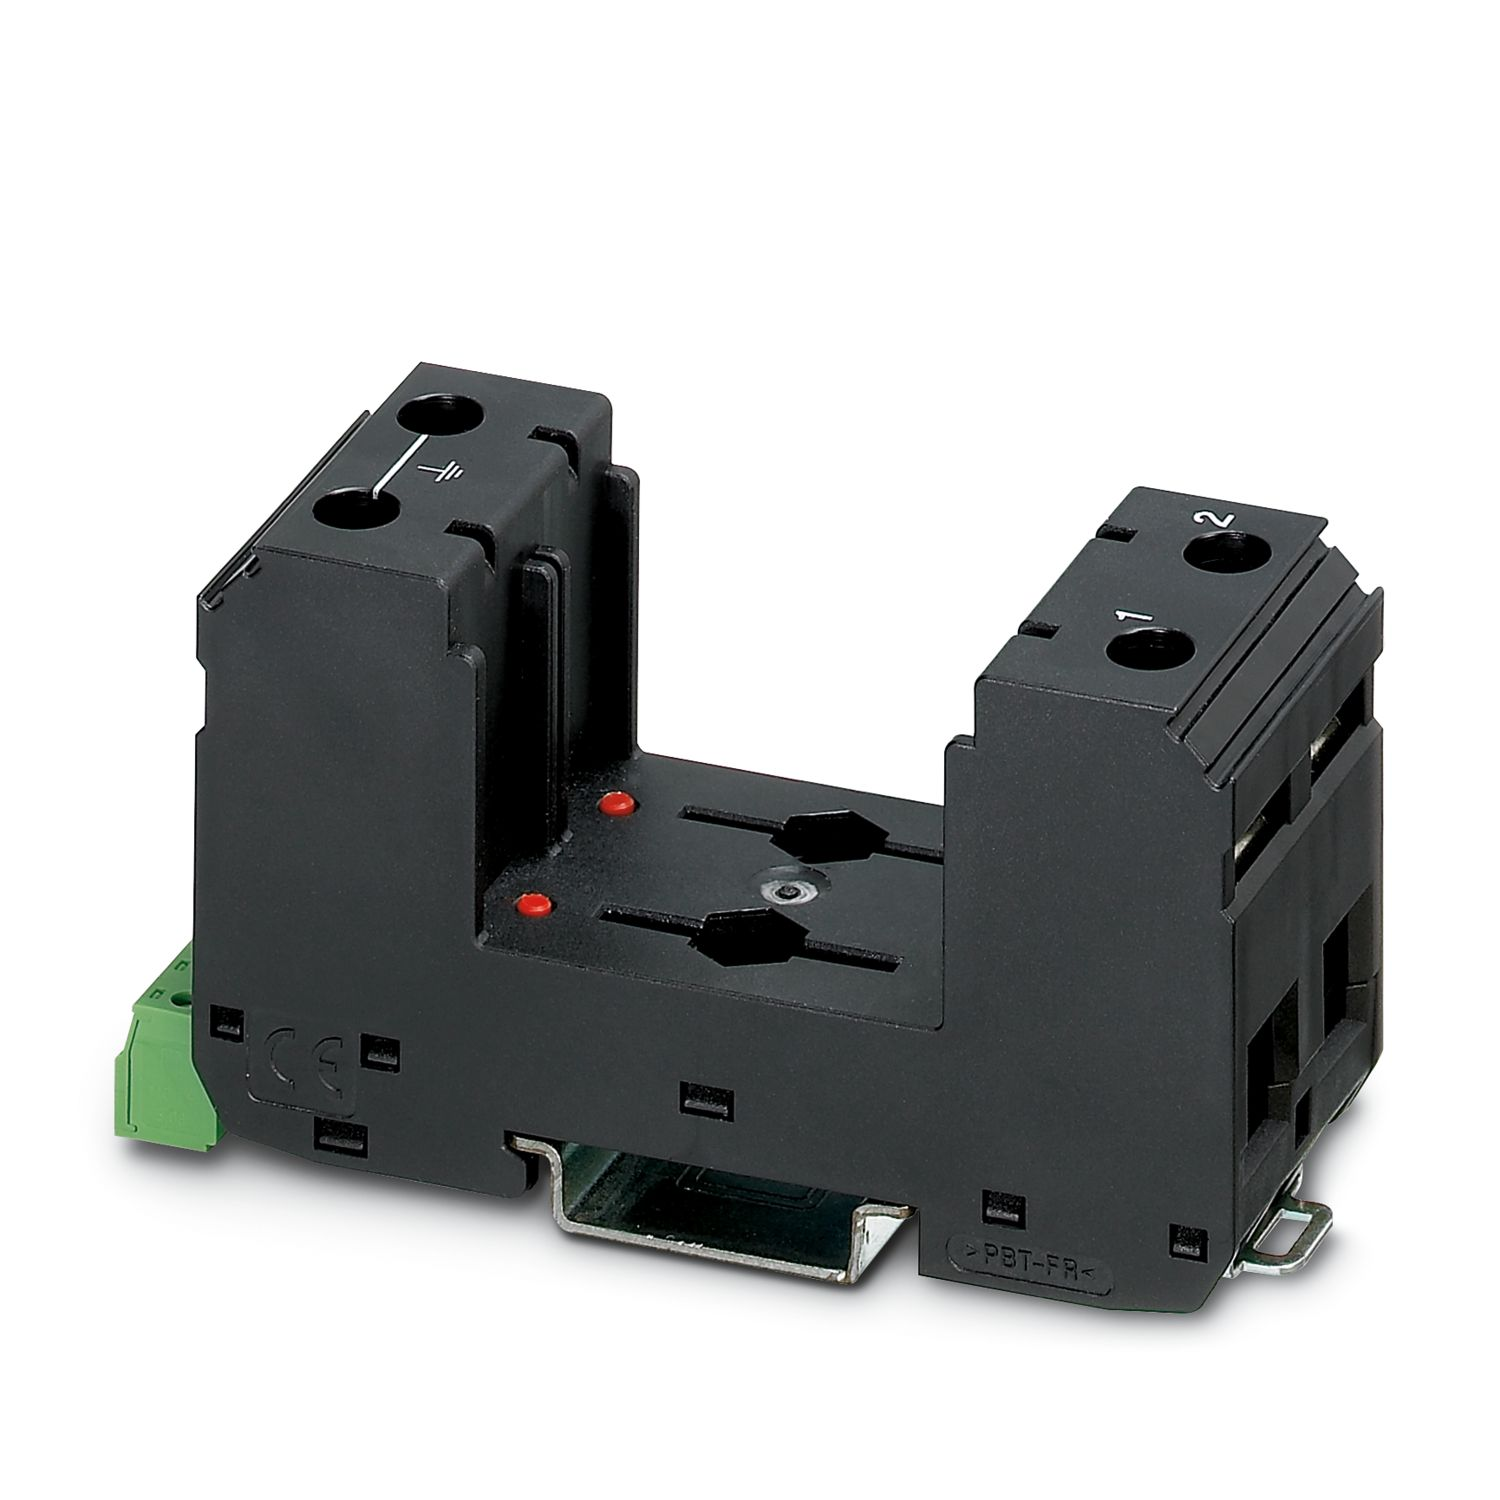
\includegraphics[width=0.92\linewidth,height=0.62\textheight,keepaspectratio]{./media/image56.png}
\captionof*{figure}{\small\itshape Figura 47. VAL-MS BE}
\addcontentsline{lof}{figure}{Figura 47. VAL-MS BE}
\label{fig:47}
\end{center}

\begin{center}
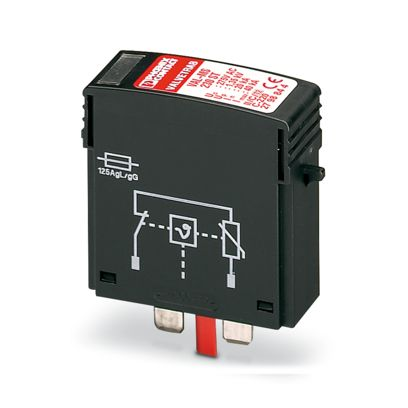
\includegraphics[width=0.92\linewidth,height=0.62\textheight,keepaspectratio]{./media/image136.png}
\captionof*{figure}{\small\itshape Figura 48. DPS - Phoenix Contact VAL-MS 230}
\addcontentsline{lof}{figure}{Figura 48. DPS - Phoenix Contact VAL-MS 230}
\label{fig:48}
\end{center}

\begin{center}
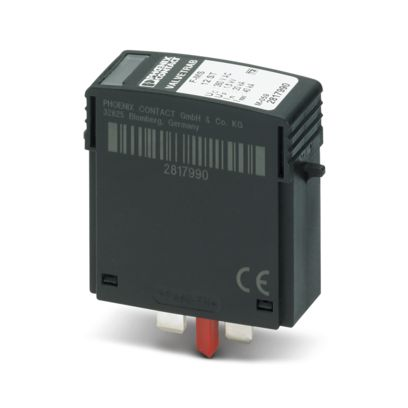
\includegraphics[width=0.92\linewidth,height=0.62\textheight,keepaspectratio]{./media/image101.png}
\captionof*{figure}{\small\itshape Figura 49. F-MS 12 ST (Fusible)}
\addcontentsline{lof}{figure}{Figura 49. F-MS 12 ST (Fusible)}
\label{fig:49}
\end{center}

El fusible interno protege el DPS contra sobrecorrientes destructivas, permitiendo su reemplazo sin comprometer el resto del sistema. Datos en la tabla 4.21.

\textbf{Interruptor Diferencial (RCD) - Schneider Electric ID K 25A 30mA}

El RCD (Residual Current Device) o Interruptor Diferencial es un dispositivo de protección que detecta diferencias entre la corriente de fase y neutro (corriente de fuga), disparando el circuito cuando esta diferencia supera un umbral (sensibilidad). Su función principal es proteger personas contra electrocución por contacto directo o indirecto con partes energizadas, en este caso protege al operario de mantenimiento. Datos en tabla 4.22.

\begin{center}
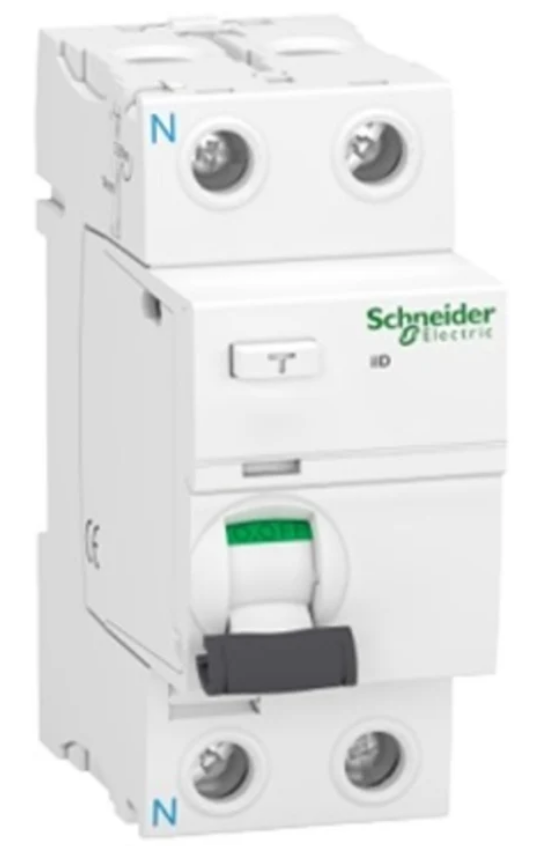
\includegraphics[width=0.92\linewidth,height=0.62\textheight,keepaspectratio]{./media/image35.png}
\captionof*{figure}{\small\itshape Figura 50. RCD - Schneider Electric ID K 25A 30mA}
\addcontentsline{lof}{figure}{Figura 50. RCD - Schneider Electric ID K 25A 30mA}
\label{fig:50}
\end{center}

Corriente peligrosa para fibrilación ventricular: \textgreater{} 50mA (\textgreater500ms) Umbral de protección seguro: 30mA y el margen de seguridad: 130ms / 30ms = 4.33 veces más rápido que el límite de seguridad.

El RCD no protege contra sobrecargas ni cortocircuitos, solo contra fugas a tierra. Por eso se instala en serie con el breaker termomagnético. En la tabla 4.23 podemos observar la lista de componentes.

\Needspace{6\baselineskip}
\captionof*{table}{\small\bfseries Tabla 4.23. Lista de componentes del sistema de alimentación}
\addcontentsline{lot}{table}{Tabla 4.23. Lista de componentes del sistema de alimentación}
\label{tbl:4.23}

\begin{longtable}[]{@{}
  >{\raggedright\arraybackslash}p{(\columnwidth - 4\tabcolsep) * \real{0.2346}}
  >{\raggedright\arraybackslash}p{(\columnwidth - 4\tabcolsep) * \real{0.3361}}
  >{\raggedright\arraybackslash}p{(\columnwidth - 4\tabcolsep) * \real{0.4293}}@{}}
\toprule
\begin{minipage}[b]{\linewidth}\raggedright
\textbf{Componente}
\end{minipage} & \begin{minipage}[b]{\linewidth}\raggedright
\textbf{Modelo seleccionado}
\end{minipage} & \begin{minipage}[b]{\linewidth}\raggedright
\textbf{Justificación técnica}
\end{minipage} \\
\begin{minipage}[b]{\linewidth}\raggedright
\textbf{Breaker}
\end{minipage} & \begin{minipage}[b]{\linewidth}\raggedright
Schneider C60N-C6
\end{minipage} & \begin{minipage}[b]{\linewidth}\raggedright
Corriente nominal 6A \textgreater{} 1.22A requerida
\end{minipage} \\
\begin{minipage}[b]{\linewidth}\raggedright
\textbf{DPS}
\end{minipage} & \begin{minipage}[b]{\linewidth}\raggedright
Phoenix VAL-MS 230
\end{minipage} & \begin{minipage}[b]{\linewidth}\raggedright
Protección contra sobretensiones; respuesta \textless100ns; corriente fuga \textless10\ensuremath{\mu}A
\end{minipage} \\
\begin{minipage}[b]{\linewidth}\raggedright
\textbf{RCD}
\end{minipage} & \begin{minipage}[b]{\linewidth}\raggedright
Schneider ID K 25A 30mA
\end{minipage} & \begin{minipage}[b]{\linewidth}\raggedright
Protección personas; sensibilidad 30mA; tiempo disparo \ensuremath{\leq}30ms
\end{minipage} \\
\begin{minipage}[b]{\linewidth}\raggedright
\textbf{UPS}
\end{minipage} & \begin{minipage}[b]{\linewidth}\raggedright
APC SMT1500IC
\end{minipage} & \begin{minipage}[b]{\linewidth}\raggedright
1000W \textgreater{} 228.4W (factor 4.38); autonomía 72 min; onda senoidal pura
\end{minipage} \\
\begin{minipage}[b]{\linewidth}\raggedright
\textbf{SMPS Principal}
\end{minipage} & \begin{minipage}[b]{\linewidth}\raggedright
S-360-24
\end{minipage} & \begin{minipage}[b]{\linewidth}\raggedright
360W \textgreater{} 191.86W (factor 1.88); eficiencia \textgreater84\%; operación al 53.3\%
\end{minipage} \\
\begin{minipage}[b]{\linewidth}\raggedright
\textbf{DC-DC 5V}
\end{minipage} & \begin{minipage}[b]{\linewidth}\raggedright
PULS CD5.051
\end{minipage} & \begin{minipage}[b]{\linewidth}\raggedright
40.75W útiles \textgreater{} 31.17W requeridos; eficiencia 81.5\%; margen 30.7\%
\end{minipage} \\
\begin{minipage}[b]{\linewidth}\raggedright
\textbf{DC-DC 12V}
\end{minipage} & \begin{minipage}[b]{\linewidth}\raggedright
PULS CD5.121
\end{minipage} & \begin{minipage}[b]{\linewidth}\raggedright
84.67W útiles \textgreater{} 6.6W requeridos; eficiencia 88.2\%
\end{minipage} \\
\midrule
\endhead
\bottomrule
\endlastfoot
\end{longtable}

\begin{center}
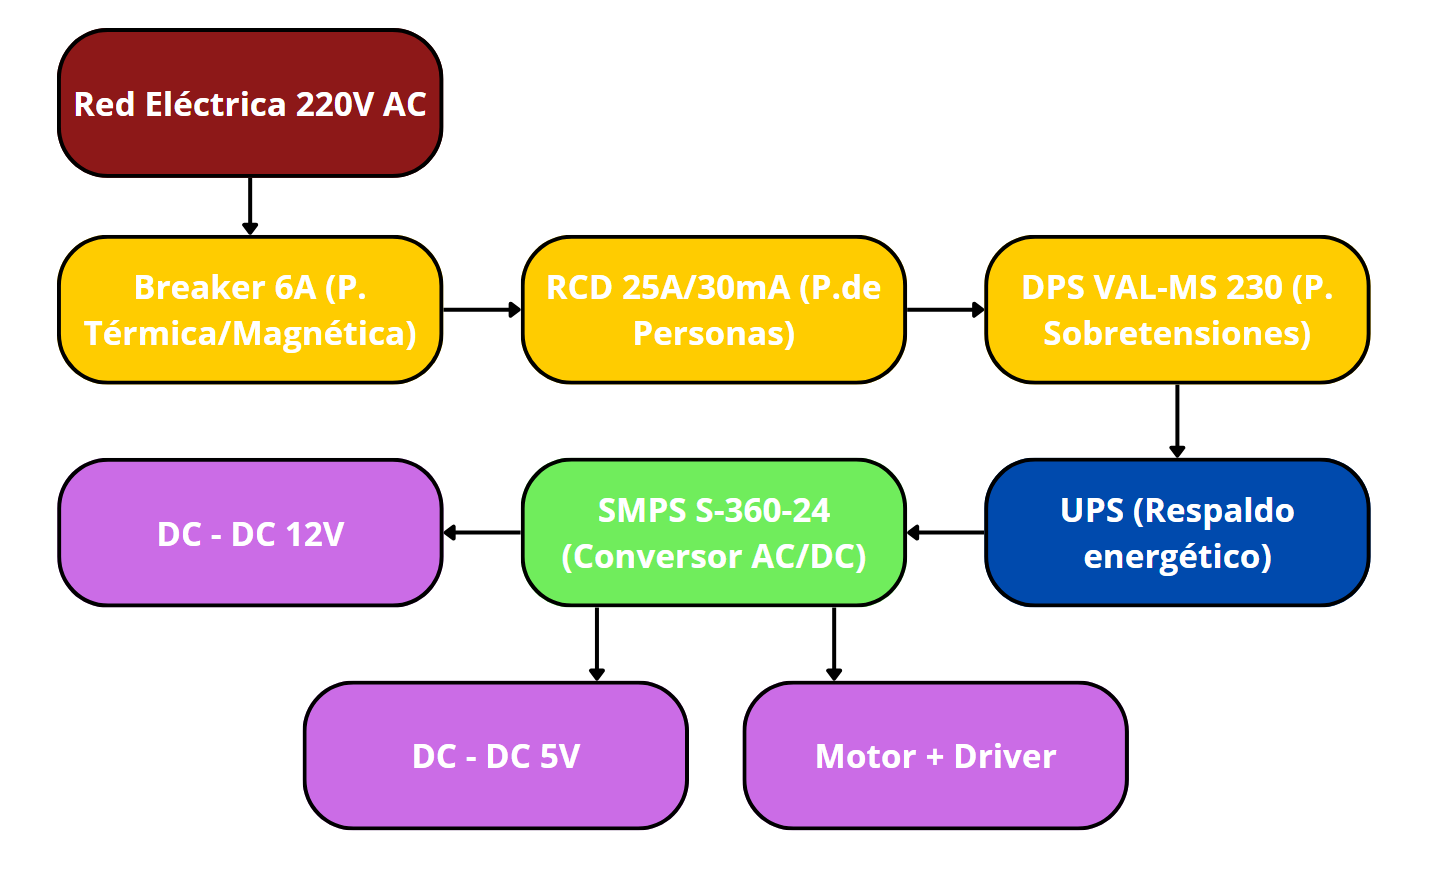
\includegraphics[width=0.92\linewidth,height=0.62\textheight,keepaspectratio]{./media/image40.png}
\captionof*{figure}{\small\itshape Figura 51. Circuito de Protecciones Eléctricas}
\addcontentsline{lof}{figure}{Figura 51. Circuito de Protecciones Eléctricas}
\label{fig:51}
\end{center}

El orden establecido en la figura 51 responde a criterios de coordinación selectiva según normas IEC 60364-5-53 y NEC Article 285. El breaker termomagnético se posiciona primero como protección primaria contra cortocircuitos y sobrecargas, limitando la corriente antes de que alcance dispositivos aguas abajo, protegiendo así al RCD de corrientes destructivas que podrían superar su capacidad de ruptura (6kA). El RCD se instala en segundo lugar para detectar corrientes de fuga a tierra una vez que el circuito está protegido contra fallas catastróficas, garantizando la seguridad de personas sin interferencias de corrientes de cortocircuito. Finalmente, el DPS se ubica aguas abajo del RCD porque durante eventos de sobretensión el DPS deriva corrientes de descarga (hasta 10kA en pulsos de 8/20\ensuremath{\mu}s) que podrían ser interpretadas como fugas y causar disparos intempestivos del RCD. Esta configuración permite que el DPS opere libremente desviando sobretensiones sin afectar la protección diferencial. Además, esta secuencia asegura que en caso de falla del DPS (cortocircuito por fin de vida útil del varistor), el breaker aguas arriba interrumpa el circuito antes de comprometer la integridad del sistema, mientras que el fusible interno F-MS 12 ST del DPS proporciona una segunda capa de protección localizada.

\section{Distribución de componentes en el gabinete modular}\label{distribuciuxf3n-de-componentes-en-el-gabinete-modular}

\subsection{Especificaciones del Gabinete Principal}\label{especificaciones-del-gabinete-principal}

El sistema de control adaptativo inteligente se aloja en un gabinete especializado que cumple con la normativa NEMA TS-2 para controladores de tráfico. Este gabinete proporciona protección IP65 contra polvo y agua, además de resistencia al impacto IK10 equivalente a 20 Joules según IEC 62262, características esenciales para soportar condiciones ambientales adversas y actos vandálicos en entornos urbanos.

Además, el acabado en pintura de polvo poliéster RAL 7035 con espesor de 70 micrones ofrece protección adicional contra corrosión. El diseño contempla un rango operativo de -40°C a +74°C según NEMA TS-2, asegurando funcionamiento continuo bajo las variaciones térmicas típicas de aplicaciones semafóricas exteriores.

El gabinete integra un sistema de rack frontal de 19 pulgadas (EIA-310-D) con altura útil de 4U que permite organización modular de componentes mediante rieles verticales separados 480 mm entre centros. Esta configuración single-frame facilita el mantenimiento al proporcionar acceso frontal a todos los elementos activos del sistema, mientras que la profundidad útil de 360 mm acomoda tanto las fuentes de alimentación como las PCBs personalizadas sin comprometer la ventilación. En la tabla 4.24 más especificaciones generales del Gabinete.

\Needspace{6\baselineskip}
\captionof*{table}{\small\bfseries Tabla 4.24. Especificaciones del Gabinete Semafórico}
\addcontentsline{lot}{table}{Tabla 4.24. Especificaciones del Gabinete Semafórico}
\label{tbl:4.24}

\begin{longtable}[]{@{}
  >{\raggedright\arraybackslash}p{(\columnwidth - 2\tabcolsep) * \real{0.3096}}
  >{\raggedright\arraybackslash}p{(\columnwidth - 2\tabcolsep) * \real{0.6904}}@{}}
\toprule
\begin{minipage}[b]{\linewidth}\raggedright
\textbf{Parámetro}
\end{minipage} & \begin{minipage}[b]{\linewidth}\raggedright
\textbf{Especificación}
\end{minipage} \\
\begin{minipage}[b]{\linewidth}\raggedright
Normativa aplicable
\end{minipage} & \begin{minipage}[b]{\linewidth}\raggedright
NEMA TS-2 (Traffic Controller Assemblies)
\end{minipage} \\
\begin{minipage}[b]{\linewidth}\raggedright
Dimensiones
\end{minipage} & \begin{minipage}[b]{\linewidth}\raggedright
600 mm x 500 mm x 600 mm
\end{minipage} \\
\begin{minipage}[b]{\linewidth}\raggedright
Material
\end{minipage} & \begin{minipage}[b]{\linewidth}\raggedright
Aluminio 5052-H32
\end{minipage} \\
\begin{minipage}[b]{\linewidth}\raggedright
Grado de protección
\end{minipage} & \begin{minipage}[b]{\linewidth}\raggedright
IP65 según IEC 60529
\end{minipage} \\
\begin{minipage}[b]{\linewidth}\raggedright
Resistencia al impacto
\end{minipage} & \begin{minipage}[b]{\linewidth}\raggedright
IK10 según IEC 62262 (20 Joules)
\end{minipage} \\
\begin{minipage}[b]{\linewidth}\raggedright
Temperatura operativa
\end{minipage} & \begin{minipage}[b]{\linewidth}\raggedright
-40°C a +74°C (NEMA TS-2)
\end{minipage} \\
\begin{minipage}[b]{\linewidth}\raggedright
Panel interno
\end{minipage} & \begin{minipage}[b]{\linewidth}\raggedright
Desmontable, rack 19'' single-frame
\end{minipage} \\
\begin{minipage}[b]{\linewidth}\raggedright
Profundidad útil
\end{minipage} & \begin{minipage}[b]{\linewidth}\raggedright
360 mm
\end{minipage} \\
\midrule
\endhead
\bottomrule
\endlastfoot
\end{longtable}

\subsection{Arquitectura del Sistema con PCBs Especializadas}\label{arquitectura-del-sistema-con-pcbs-especializadas}

El sistema implementa dos PCBs personalizadas que trabajan en conjunto para centralizar la distribución de energía y el procesamiento inteligente. La PCB de Distribución actúa como hub central de voltaje, recibiendo las líneas reguladas de 12VDC (calibre 18 AWG) y 5VDC (calibre 18 AWG) desde los convertidores PULS CD5.121 y CD5.051 respectivamente, y distribuyendolas mediante conectores PAD hacia los diferentes subsistemas. Esta PCB integra además componentes críticos de adquisición de datos: el conversor analógico-digital MCP3008 de 8 canales que se comunica con la Raspberry Pi mediante bus SPI, el conversor ADC para procesamiento de señales analógicas, y conectores PAD para sensores y demás componentes.

El motor PAP NEMA 23 recibe alimentación directa de 24VDC desde la SMPS mediante cable calibre 16 AWG hacia el driver DM542T, que a su vez se controla digitalmente desde la Raspberry Pi a través de señales paso/dirección transportadas por la PCB de Distribución. Los sensores externos como el ultrasónico de presencia y el de temperatura y corriente se conectan mediante conectores PAD soldados en la PCB de Controlador. Todo lo comentado se puede evidenciar en la Figura 52.

\begin{center}
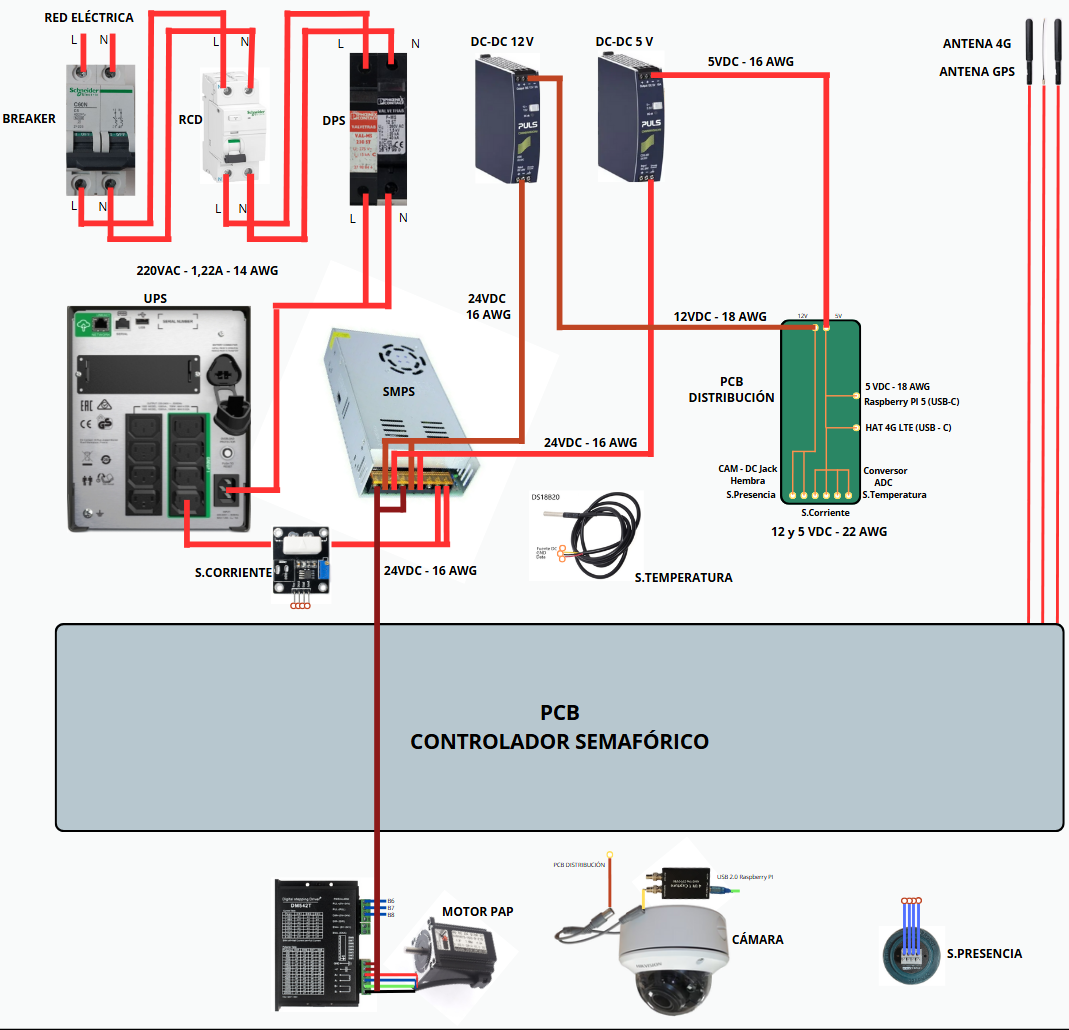
\includegraphics[width=0.92\linewidth,height=0.62\textheight,keepaspectratio]{./media/image44.png}
\captionof*{figure}{\small\itshape Figura 52. Conexiones de Potencia y Control IoT}
\addcontentsline{lof}{figure}{Figura 52. Conexiones de Potencia y Control IoT}
\label{fig:52}
\end{center}

Especificando un poco más sobre la PCB Controlador Semafórico, en esta encontramos acoplada la Raspberry Pi 5, mediante sus pines, su alimentación será mediante el PCB de Distribución brindándole los 25W que necesita, en uno de los USB 3.0 se pondrá el Coral y en el otro junto a un conversor se pondrá al HAT 4G LTE, esta será la comunicación de datos, sin embargo la alimentación del HAT también será por la PCB de distribución, la posición del HAT será en la parte superior del Raspberry PI mediante sus Pines GPIO, estas conexiones se evidencian en la Figura 53.

\begin{center}
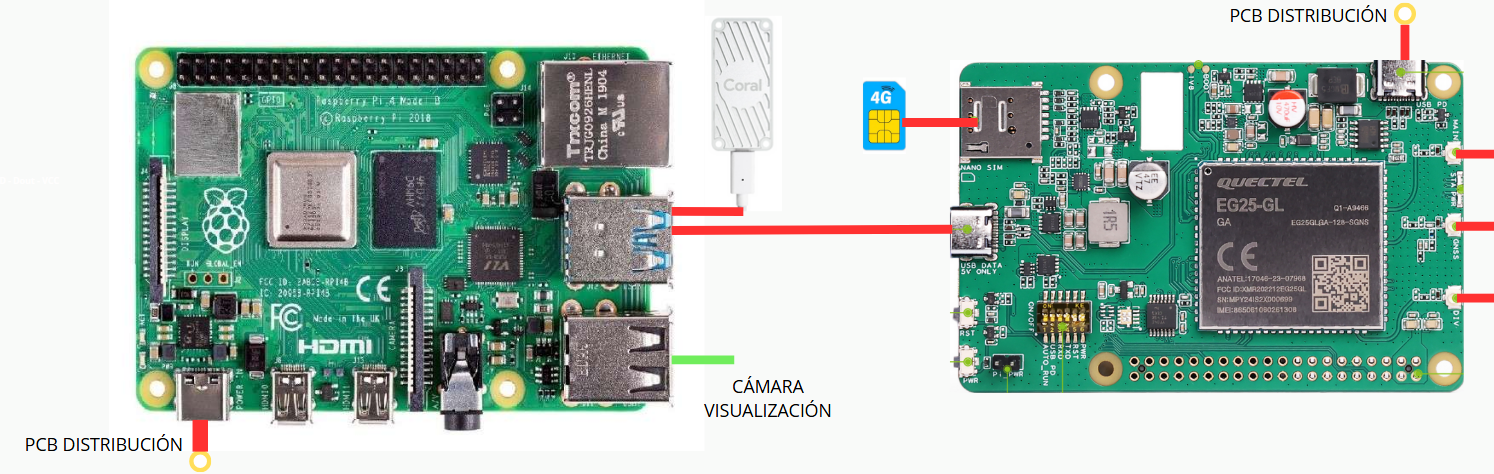
\includegraphics[width=0.92\linewidth,height=0.62\textheight,keepaspectratio]{./media/image107.png}
\captionof*{figure}{\small\itshape Figura 53. Conexiones Raspberry PI y HAT 4G LTE en la PCB Controlador Semafórico}
\addcontentsline{lof}{figure}{Figura 53. Conexiones Raspberry PI y HAT 4G LTE en la PCB Controlador Semafórico}
\label{fig:53}
\end{center}

Siguiendo con las partes que se encuentran dentro de la PCB Controlador, encontramos el Conversor de 8 entradas y salidas que permite modificar las señales de 5V a 3.3V y viceversa, este se conectará al Raspberry PI por los cables Verdes, a los Pads enfocados en el Sensor de Temperatura por los cables Azules, al Driver del Motor Pap por los cables Azules Gruesos y por último a la PCB de Distribución por los cables Rojos. De igual forma para la conexión al Sensor de Temperatura usaremos unos PADS enfocados que cubran Data, GND y VCC correspondientes, con una resistencia estratégica para cubrir funcionamiento, todo lo mencionado se evidencia en la Figura 54.

\begin{center}
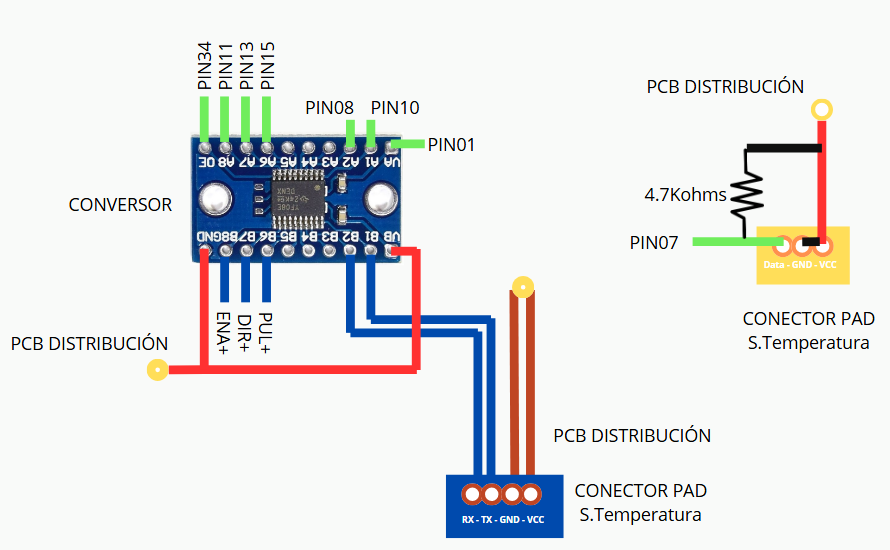
\includegraphics[width=0.92\linewidth,height=0.62\textheight,keepaspectratio]{./media/image126.png}
\captionof*{figure}{\small\itshape Figura 54. Conversor Digital y Pads para Sensores ubicados en la PCB Controlador}
\addcontentsline{lof}{figure}{Figura 54. Conversor Digital y Pads para Sensores ubicados en la PCB Controlador}
\label{fig:54}
\end{center}

De igual forma el ADC necesario para el Sensor de Corriente y los PADS de conexión para el mismo estarán integrados en la PCB Controladora. Evidencia en la Figura 55.

\begin{center}
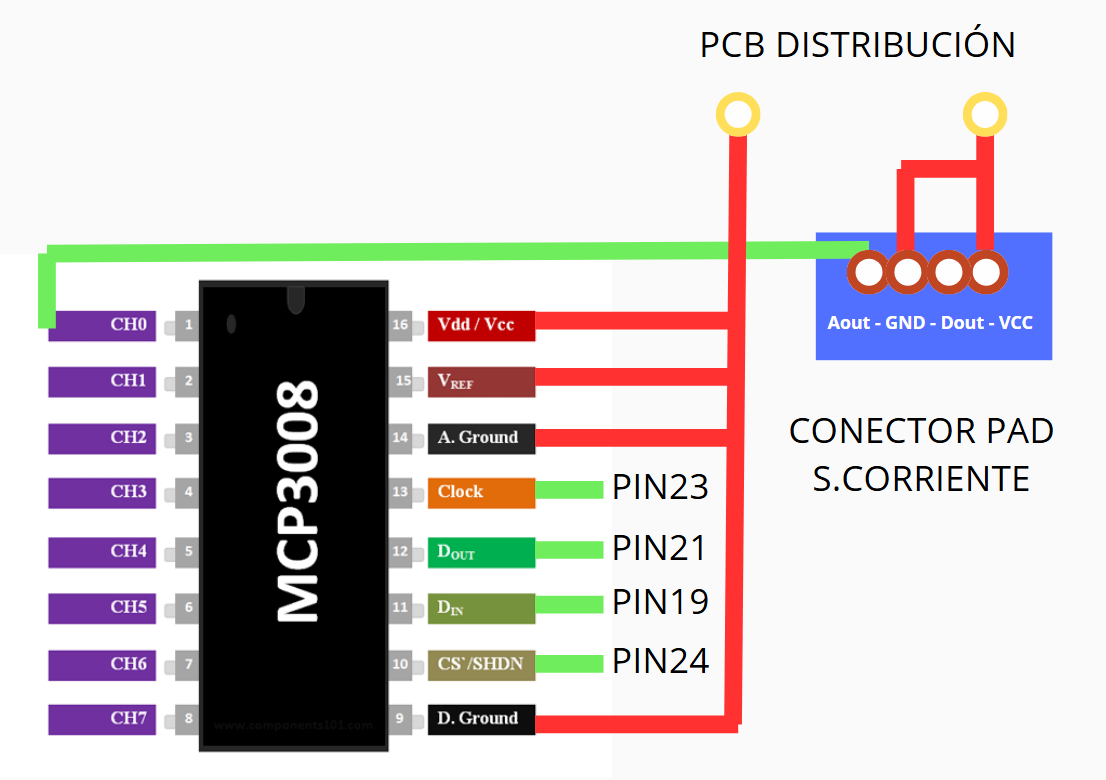
\includegraphics[width=0.92\linewidth,height=0.62\textheight,keepaspectratio]{./media/image148.png}
\captionof*{figure}{\small\itshape Figura 55. ADC y Pads para Sensores ubicados en la PCB Controlador}
\addcontentsline{lof}{figure}{Figura 55. ADC y Pads para Sensores ubicados en la PCB Controlador}
\label{fig:55}
\end{center}

Por último, la comunicación de la Raspberry PI con la cámara se realizará mediante el USB 2.0 De la Raspberry y la alimentación de la cámara se realizará directamente con la PCB de Distribución. Evidencia en la Figura 56.

\begin{center}
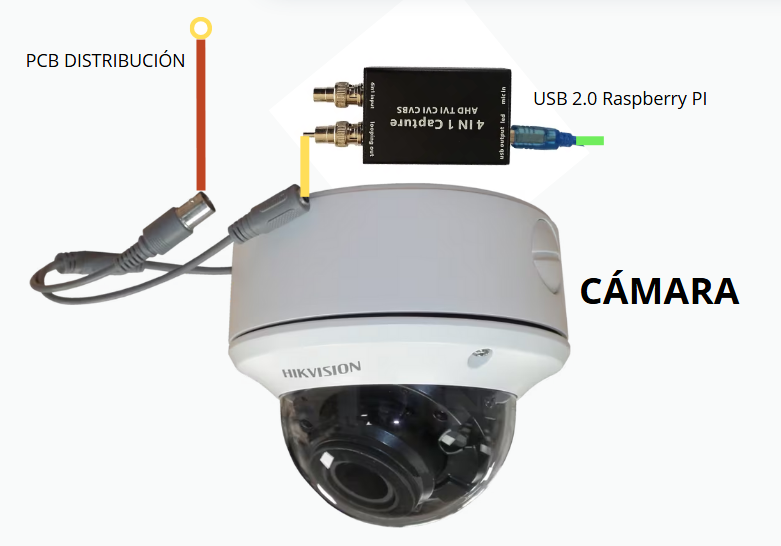
\includegraphics[width=0.92\linewidth,height=0.62\textheight,keepaspectratio]{./media/image24.png}
\captionof*{figure}{\small\itshape Figura 56. Conexión Cámara, alimentación, Raspberry PI}
\addcontentsline{lof}{figure}{Figura 56. Conexión Cámara, alimentación, Raspberry PI}
\label{fig:56}
\end{center}

\subsection{Distribución por Zonas Funcionales en Rack 19''}\label{distribuciuxf3n-por-zonas-funcionales-en-rack-19}

La organización vertical del rack sigue principios de separación electromagnética y térmica, agrupando componentes según su función y requisitos de disipación de calor. La unidad 1U superior aloja las protecciones eléctricas montadas en riel DIN según la secuencia establecida en el diagrama de la Figura 48: el breaker Schneider C60N-C6 actúa como primera línea de defensa contra sobrecargas y cortocircuitos, seguido del RCD ID K 25A/30mA que protege al personal de mantenimiento contra descargas eléctricas, y finalmente el DPS Phoenix VAL-MS 230 que suprime sobretensiones transitorias antes de que alcancen equipos sensibles aguas abajo. El cable de entrada AC 220V calibre 14 AWG transporta aproximadamente 1.22A desde la red eléctrica, valor significativamente inferior a la capacidad nominal del breaker de 6A. Graficado en la Figura 57.

\begin{center}
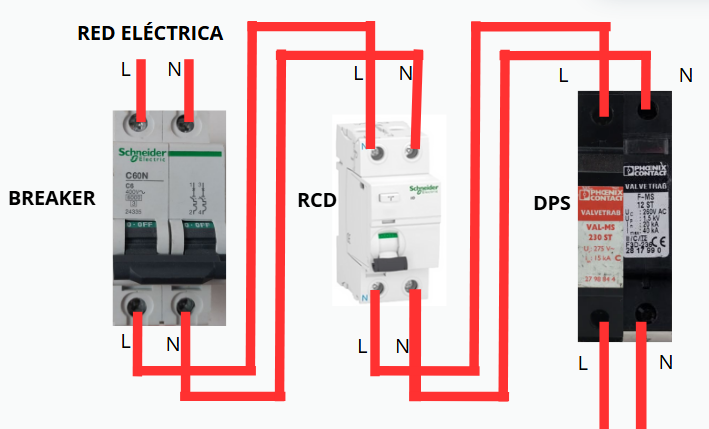
\includegraphics[width=0.92\linewidth,height=0.62\textheight,keepaspectratio]{./media/image2.png}
\captionof*{figure}{\small\itshape Figura 57. Conexión Breaker - RCD - DPS}
\addcontentsline{lof}{figure}{Figura 57. Conexión Breaker - RCD - DPS}
\label{fig:57}
\end{center}

Las unidades 2U-3U centrales concentran la infraestructura de alimentación sobre bandeja perforada de aluminio que permite ventilación natural convectiva. El UPS de 1500VA/1000W recibe la línea protegida y mantiene continuidad operativa durante interrupciones de red mediante sus baterías AGM de 2\ensuremath{\times}12V 12Ah que proporcionan autonomía calculada de 72 minutos bajo carga nominal del sistema. La salida del UPS alimenta la SMPS S-360-24 que genera el bus principal de 24VDC mediante conversión AC/DC. Desde este bus de 24VDC se derivan tres líneas principales mediante cables calibre 16 AWG: una hacia el convertidor DC-DC PULS CD5.121 que genera 12VDC para cámara y sensor ultrasónico, otra hacia el convertidor DC-DC PULS CD5.051 que produce 5VDC para la PCB Controlador, y una tercera línea directa hacia el driver DM542T del motor PAP NEMA 23. El sensor DS18B20 conectado a PADs en la PCB Controlador monitorea temperatura ambiente para activación de alarmas si se detecta sobrecalentamiento anormal.

La unidad U4 aloja las dos PCBs personalizadas que constituyen el núcleo del sistema inteligente. La \textbf{PCB de Distribución} ubicada en el nivel 4U actúa como hub centralizado que recibe las líneas reguladas de 12VDC y 5VDC desde los convertidores PULS, redistribuyéndolas mediante conectores PAD hacia los subsistemas que lo requieren según se muestra en la Figura 49.

La \textbf{PCB Controlador Semafórico} montada en el nivel 4U integra la Raspberry Pi 5 acoplada directamente mediante sus pines GPIO, recibiendo los 25W de alimentación necesarios desde la PCB de Distribución. Sobre la Raspberry Pi se monta el HAT 4G LTE con módulo QUECTEL EG25-G conectado mediante los pines GPIO superiores, formando un ensamblaje apilado compacto que minimiza el espacio ocupado en el rack.

Además, en la unidad U4 se contendrá el driver de motor DM542T que recibe alimentación de potencia de 24VDC directamente desde la SMPS mediante cable calibre 16 AWG capaz de transportar los 4.2A requeridos durante operación continua del motor PAP. Las señales de control digital de paso y dirección llegan desde la Raspberry Pi a través del conversor de nivel lógico en la PCB Controlador, pasando por la PCB de Distribución que actúa como punto de interconexión centralizado antes de alcanzar los terminales de entrada del driver. El sensor ultrasónico URM06 de presencia se conecta mediante PADs en la PCB Controlador que proporcionan tanto su alimentación de 12VDC como la interfaz serial RX-TX para comunicación bidireccional. Tanto el Sensor ultrasónico URM06 y la cámara se encontrarán en la parte inferior del Gabinete teniendo contacto directo con el exterior para cubrir sus funciones de vigilancia y detección. Las antenas del HAT 4G LTE y el módulo GPS atraviesan el panel superior del gabinete mediante conectores SMA separados 100mm entre sí para minimizar acoplamiento electromagnético que podría degradar sensibilidad de recepción. Distribución Figura 58.

\begin{center}
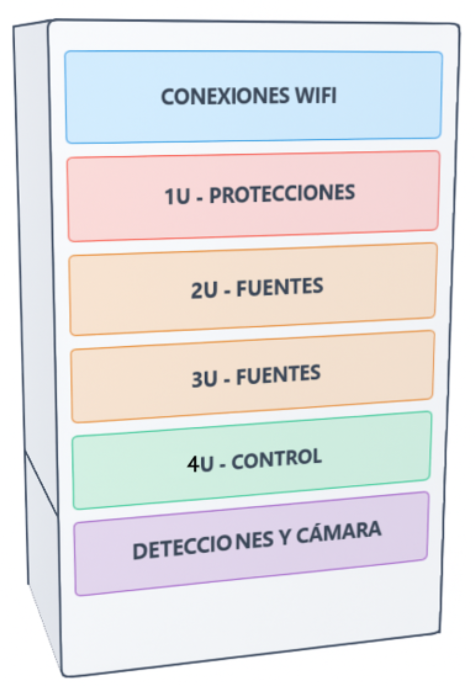
\includegraphics[width=0.92\linewidth,height=0.62\textheight,keepaspectratio]{./media/image22.png}
\captionof*{figure}{\small\itshape Figura 58. Distribución en el Rack}
\addcontentsline{lof}{figure}{Figura 58. Distribución en el Rack}
\label{fig:58}
\end{center}

\section{Diagramas esquemáticos}\label{diagramas-esquemuxe1ticos}

\subsection{Diagrama esquemático Sistema de alimentación y protecciones}\label{diagrama-esquemuxe1tico-sistema-de-alimentaciuxf3n-y-protecciones}

El esquemático de la Figura 59 representa la arquitectura completa del sistema de alimentación, mostrando la secuencia de protecciones y conversión de energía desde la red AC hasta las cargas DC. La entrada de 220V AC 60Hz atraviesa primero el breaker termomagnético Schneider C60N-C6 que protege contra sobrecargas y cortocircuitos mediante disparo a 6A nominal. Este dispositivo actúa como primera barrera de protección, interrumpiendo el circuito ante corrientes anormales que excedan su curva de disparo Tipo C (5-10\ensuremath{\times} la corriente nominal para disparo magnético instantáneo).

Aguas abajo del breaker se ubica el DPS Phoenix Contact VAL-MS 230 que suprime sobretensiones transitorias desviándolas a tierra mediante varistores de óxido metálico. Su nivel de protección de 1.5kV limita picos de voltaje antes de que alcancen equipos sensibles, mientras que su tiempo de respuesta inferior a 100ns garantiza actuación efectiva ante frentes de onda rápidos típicos de descargas atmosféricas o conmutación de cargas inductivas en la red. El RCD Schneider ID K 25A 30mA se posiciona después del DPS para detectar corrientes de fuga a tierra superiores a 30mA, protegiendo al personal de mantenimiento contra electrocución por contacto indirecto con partes metálicas energizadas accidentalmente.

El UPS de 1500VA/1000W recibe la línea protegida y proporciona respaldo energético mediante baterías AGM de 2\ensuremath{\times}12V 12Ah que ofrecen autonomía de 72 minutos bajo carga nominal del sistema. Su salida de onda senoidal pura alimenta la SMPS S-360-24 que convierte 220V AC a 24V DC con potencia nominal de 360W y eficiencia superior al 84\%. Este bus de 24VDC constituye el nivel de distribución primario desde el cual se derivan tres líneas: una alimenta directamente el motor PAP NEMA 23 y su driver DM542T, mientras que las otras dos alimentan los convertidores DC-DC PULS que generan voltajes secundarios.

El convertidor PULS CD5.121 transforma 24VDC a 12VDC con capacidad de 8A (96W), alimentando la cámara y el sensor ultrasónico mediante la PCB de Distribución. El convertidor PULS CD5.051 genera 5VDC con capacidad de 10A (50W), proporcionando alimentación para la Raspberry Pi 5, HAT 4G LTE y demás componentes de menor consumo.\\
\strut \\
\begin{center}
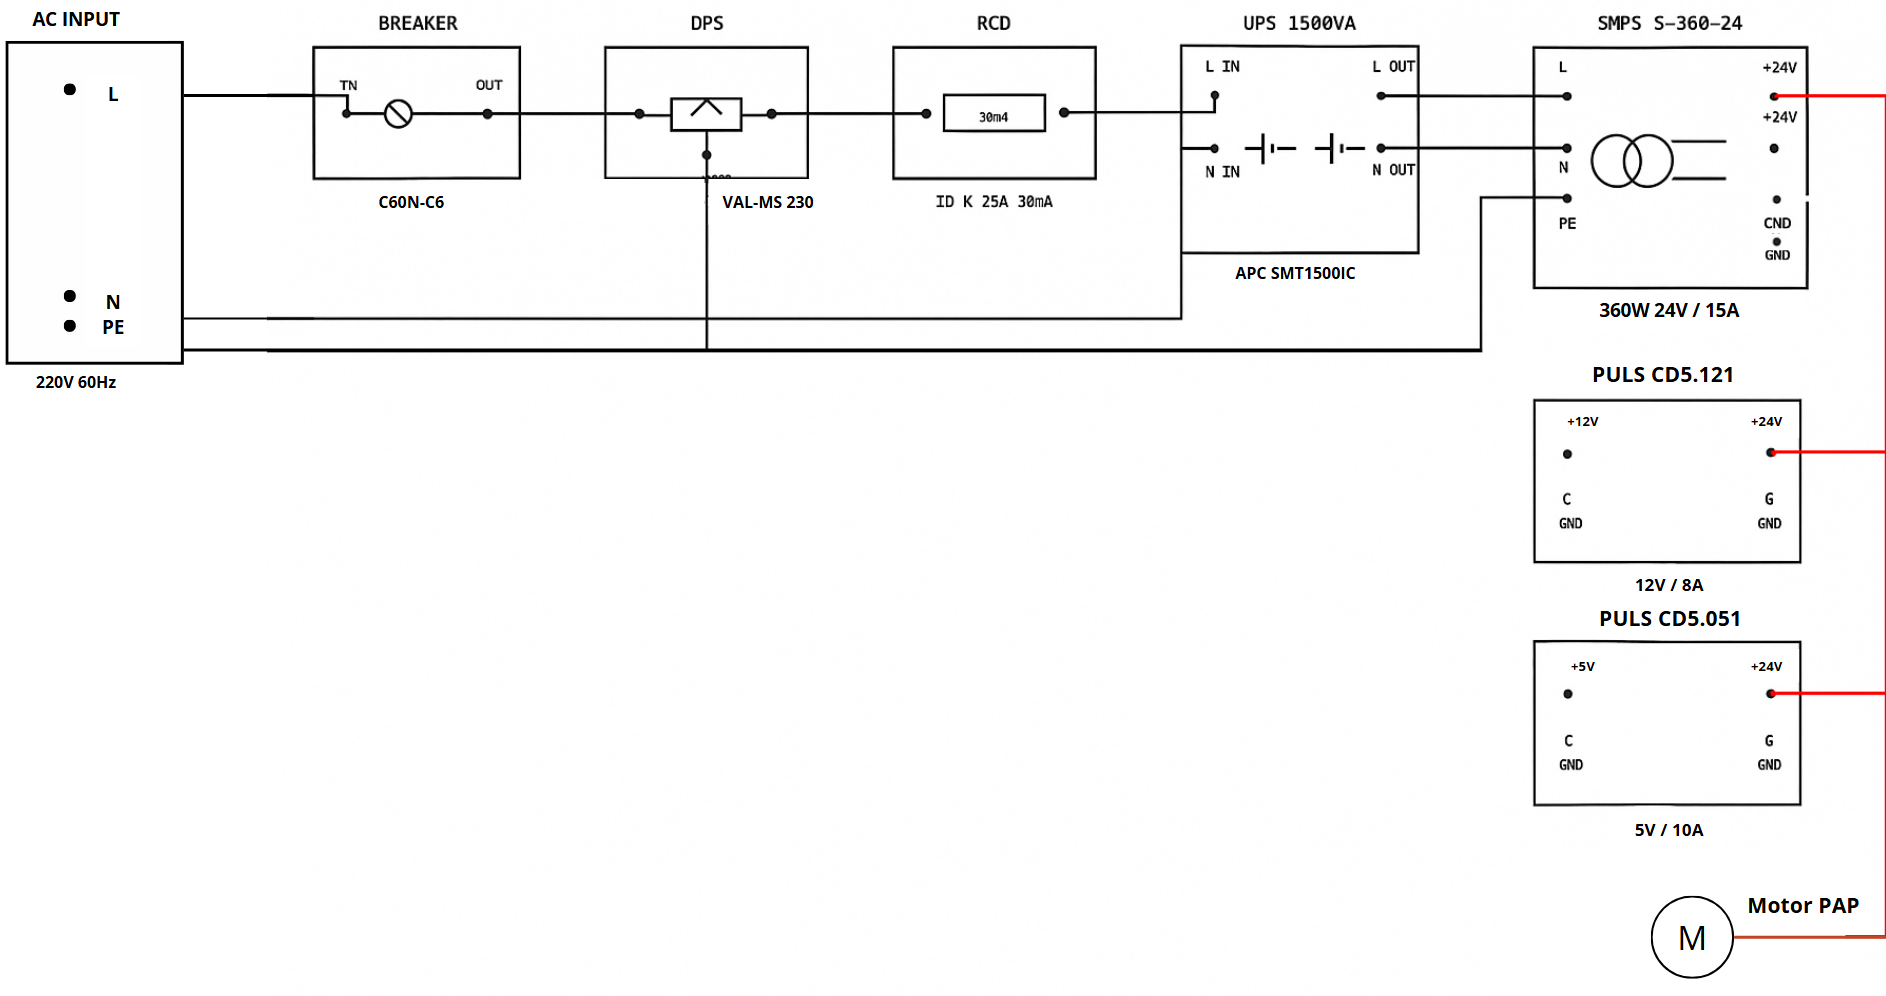
\includegraphics[width=0.92\linewidth,height=0.62\textheight,keepaspectratio]{./media/image117.png}
\captionof*{figure}{\small\itshape Figura 59. Esquemático Alimentación y Protección}
\addcontentsline{lof}{figure}{Figura 59. Esquemático Alimentación y Protección}
\label{fig:59}
\end{center}

\subsection{Diagrama esquemático y PCB de Distribución de Alimentación}\label{diagrama-esquemuxe1tico-y-pcb-de-distribuciuxf3n-de-alimentaciuxf3n}

La PCB de Distribución implementa topología en estrella con filtrado multicapa para asegurar calidad de alimentación (Sierra Circuits, 2025). El esquemático de 5V mostrado en la Figura 60 incorpora protección de entrada mediante diodo rectivador TVS P6KE6.8CA bidireccional (600W pico) que limita sobretensiones a 6.8V. El fusible 3557-2 de 10A proporciona protección contra cortocircuitos con margen sobre la corriente máxima de 6.23A, permitiendo reemplazo rápido sin desoldar componentes.

El banco de filtrado combina capacitores electrolíticos de 1000\ensuremath{\mu}F y 470\ensuremath{\mu}F para supresión de baja frecuencia (DC-100kHz), complementados por cerámicos de 1\ensuremath{\mu}F y 0.1\ensuremath{\mu}F que extienden filtrado hasta frecuencias superiores a 10MHz (Arshon Technology, 2025). El inductor AIAP-03-121K de 120\ensuremath{\mu}H forma filtro LC con frecuencia de corte calculada de 46Hz, atenuando rizado del convertidor DC-DC (100kHz) a niveles menores de 10mVpp. Las salidas individuales incorporan capacitores localizados: 470\ensuremath{\mu}F para Raspberry Pi 5 que sostiene transitorios de 3-5A durante picos computacionales, y 100\ensuremath{\mu}F para HAT 4G LTE dimensionado según su consumo de 0.6A con picos de 2A durante transmisión GSM.

El circuito de 12V mostrado en la Figura 61 utiliza arquitectura similar con componentes ajustados: diodo TVS SMAJ12A unidireccional (400W), fusible 0453005.MR de 5A, y banco de capacitores de 1000\ensuremath{\mu}F, 470\ensuremath{\mu}F y 100\ensuremath{\mu}F con voltaje nominal de 35V que proporciona margen de 2.9\ensuremath{\times} sobre el voltaje de operación. El ferrite bead BLM21PG121SN1D (120\ensuremath{\Omega} @ 100MHz) reemplaza al inductor, optimizando supresión de EMI mediante disipación resistiva del ruido de alta frecuencia generado por la cámara. Las salidas se simplifican a dos principales: cámara con 100\ensuremath{\mu}F de filtrado local, y sensor ultrasónico.

\begin{center}
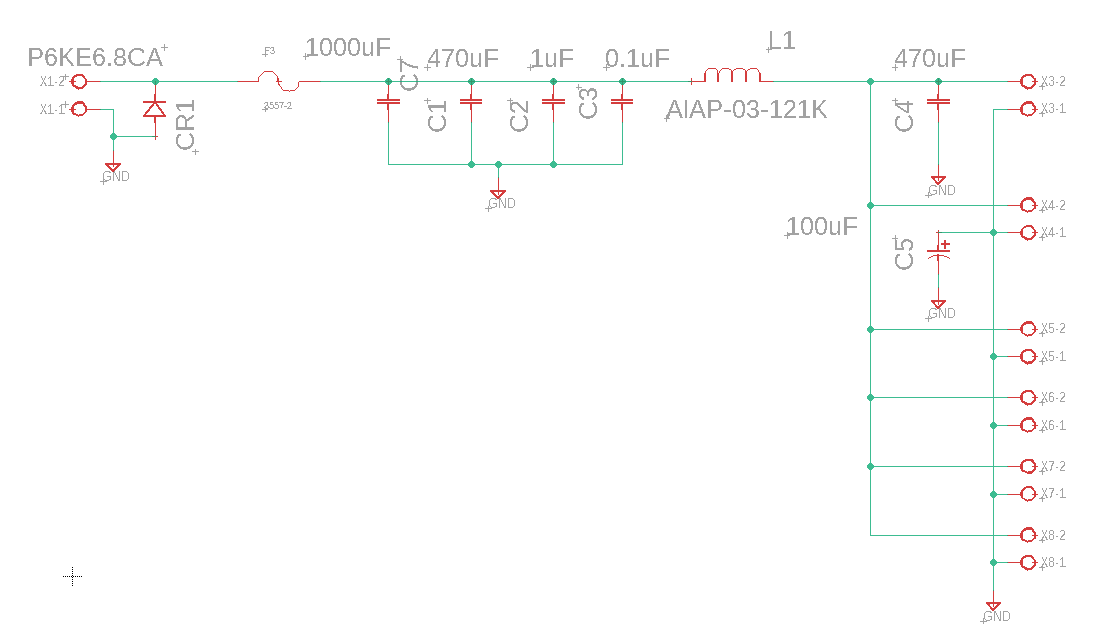
\includegraphics[width=0.92\linewidth,height=0.62\textheight,keepaspectratio]{./media/image77.png}
\captionof*{figure}{\small\itshape Figura 60. Esquemático Distribución 5V}
\addcontentsline{lof}{figure}{Figura 60. Esquemático Distribución 5V}
\label{fig:60}
\end{center}

\begin{center}
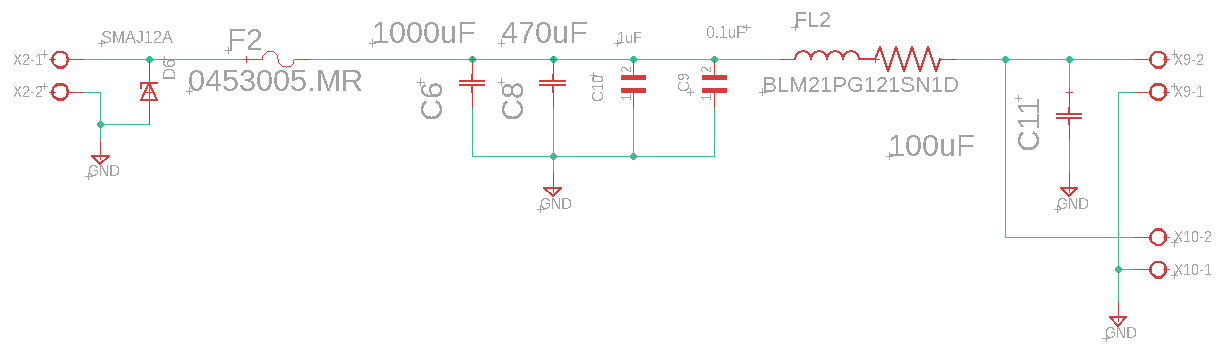
\includegraphics[width=0.92\linewidth,height=0.62\textheight,keepaspectratio]{./media/image69.png}
\captionof*{figure}{\small\itshape Figura 61. Esquemático Distribución 12V}
\addcontentsline{lof}{figure}{Figura 61. Esquemático Distribución 12V}
\label{fig:61}
\end{center}

La PCB mostrada en la Figura 62 implementa diseño de dos capas con \textbf{cobre de 2 oz (70\ensuremath{\mu}m de espesor)} que permite utilizar pistas más estrechas manteniendo capacidad de corriente adecuada (AdvancedPCB, 2024). El uso de 2 oz en lugar del estándar de 1 oz duplica el área de sección transversal del conductor, reduciendo la resistencia DC a la mitad y duplicando la capacidad de disipación térmica por conducción hacia el sustrato de FR4.

Las pistas de \textbf{5V utilizan ancho de 2mm} para transportar corriente nominal de \textbf{6.5A} con elevación térmica calculada inferior a 15°C sobre temperatura ambiente.. Las pistas de \textbf{12V utilizan ancho de 1.5mm} para transportar corriente nominal de \textbf{1.5A}, valor significativamente inferior a la capacidad de aproximadamente 5-6A que puede manejar esta geometría con cobre de 2 oz, resultando en margen holgado.

La disposición de componentes sigue flujo direccional de izquierda a derecha, con entradas de alimentación de 5V y 12V concentradas en el borde izquierdo mediante conectores de doble terminal que facilitan conexión desde los convertidores PULS. Los elementos de protección (TVS P6KE6.8CA y SMAJ12A, diodos CR1, fusibles 3557-2 y 0453005.MR) se ubican inmediatamente después de las entradas en la zona izquierda-central. Los capacitores electrolíticos grandes de 1000\ensuremath{\mu}F y 470\ensuremath{\mu}F se posicionan en la región central minimizando inductancia del lazo entre punto de entrada y primer elemento de filtrado, mientras que el inductor AIAP-03-121K para 5V ocupa posición central aprovechando su mayor tamaño físico.

Los capacitores cerámicos de 1\ensuremath{\mu}F y 0.1\ensuremath{\mu}F se distribuyen estratégicamente cerca de cada conector de salida en el borde derecho proporcionando desacoplamiento localizado que atenúa transitorios antes de que alcancen las cargas (KSN PCB, n.d.). La salida ``12V Cam'' se posiciona en el borde inferior derecho separada físicamente de las líneas de 5V minimizando acoplamiento capacitivo entre buses de diferente voltaje.

Las vías de conexión a tierra se distribuyen cada 10-15mm alrededor de los capacitores creando múltiples rutas paralelas de retorno que reducen impedancia efectiva en alta frecuencia.

\begin{center}
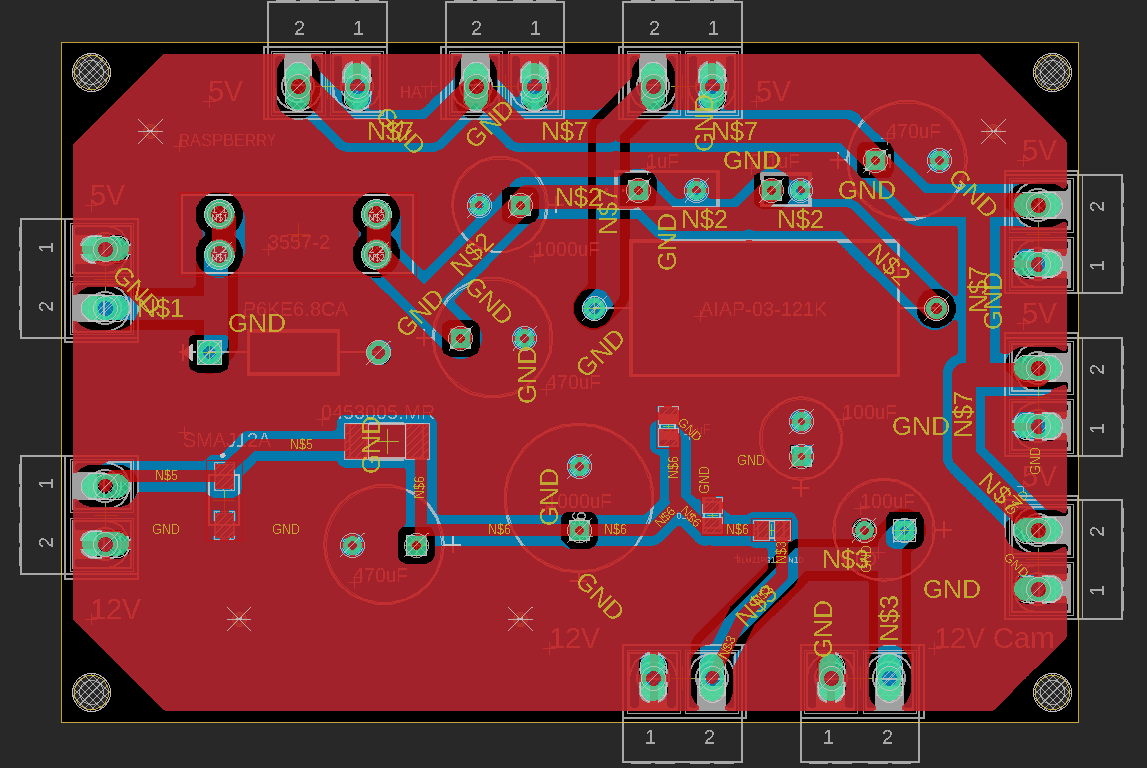
\includegraphics[width=0.92\linewidth,height=0.62\textheight,keepaspectratio]{./media/image8.png}
\captionof*{figure}{\small\itshape Figura 62. PCB de Distribución}
\addcontentsline{lof}{figure}{Figura 62. PCB de Distribución}
\label{fig:62}
\end{center}

\subsection{Diagrama esquemático y PCB Controlador Semafórico}\label{diagrama-esquemuxe1tico-y-pcb-controlador-semafuxf3rico}

El esquemático de la PCB Controlador Semafórico, ilustrado en la Figura 63, integra las interfaces necesarias para conectar sensores, actuadores y módulos periféricos a la Raspberry Pi 5, asegurando compatibilidad de voltajes y distribución eficiente de señales. Esta PCB actúa como un intermediario que facilita la conexión de componentes de 5V con los pines GPIO de la Raspberry Pi, que operan a 3.3V, evitando daños por incompatibilidad de niveles lógicos (Little Bird Electronics, n.d.).

Para el sensor de temperatura, el pin GPIO 4 de la Raspberry Pi se conecta directamente al pin de datos del sensor , con una resistencia pull-up de 4.7k\ensuremath{\Omega} entre el pin de datos y la línea de 5V, como se recomienda para estabilizar la comunicación One-Wire y garantizar lecturas precisas (Raspberry Pi Forums, 2023). El sensor de corriente se conecta mediante su salida analógica (AOUT), conectada al canal de entrada del convertidor analógico-digital (ADC) MCP3008, que utiliza los pines GPIO 8 (CE0), 9 (MISO), 10 (MOSI) y 11 (SCLK) para comunicación SPI. Este ADC opera a 3.3V para compatibilidad con la Raspberry Pi,

Las alimentaciones de los sensores se derivan directamente de la PCB de Distribución, con todas las tierras (GND) unificadas al plano de GND común para minimizar bucles de tierra y ruido. Un convertidor de nivel lógico bidireccional se emplea para adaptar señales de 5V a 3.3V. El sensor de presencia de individuo cerca del Gabinete se conecta a través de sus pines TX/RX a los canales de alto voltaje del convertidor, con las salidas de bajo voltaje enlazadas a los GPIO 14 y 15 de la Raspberry Pi. De manera similar, el driver del motor paso a paso (DM542T) se interfaces mediante sus pines DIR, PUL y ENA a los canales de 5V del convertidor, con las salidas correspondientes a los GPIO 17, 22 y 27, buscando asegurar una alimentación segura para la Raspberry Pi.

La bornera inferior de la PCB sirve como salida para conectar el driver del motor y el sensor de presencia, utilizando conectores de tornillo de 4 y 5 pines para una conexión robusta y fácil mantenimiento. La cámara se conecta directamente al puerto USB 2.0 de la Raspberry Pi, mientras que el puerto USB 3.0 se reserva para el acelerador de IA Google Coral y las interfaces de datos del HAT 4G LTE, optimizando el ancho de banda disponible. La alimentación general de la PCB Controlador se suministra desde la PCB de Distribución, utilizando cobre de 1 oz y pistas de 0.4 mm de ancho para las rutas de datos, lo cual es suficiente para corrientes bajas y señales digitales. Figura 64.

La Raspberry Pi se apila directamente sobre el HAT 4G LTE mediante sus pines hembra, y este conjunto se monta en los pines hembra de la PCB Controlador, pues el HAT en el lado contrario a sus pines hembra trae una replica de los pines macho de la raspberry Pi, por lo que conectamos este componente directamente a los pines hembra de la PCB Controladora , permitiendo una distribución simultánea de señales de datos, GPS y WiFi. Esta configuración de apilamiento sigue las mejores prácticas para HATs, asegurando alineación mecánica y eléctrica sin interferencias (BC Robotics, n.d.).

\begin{center}
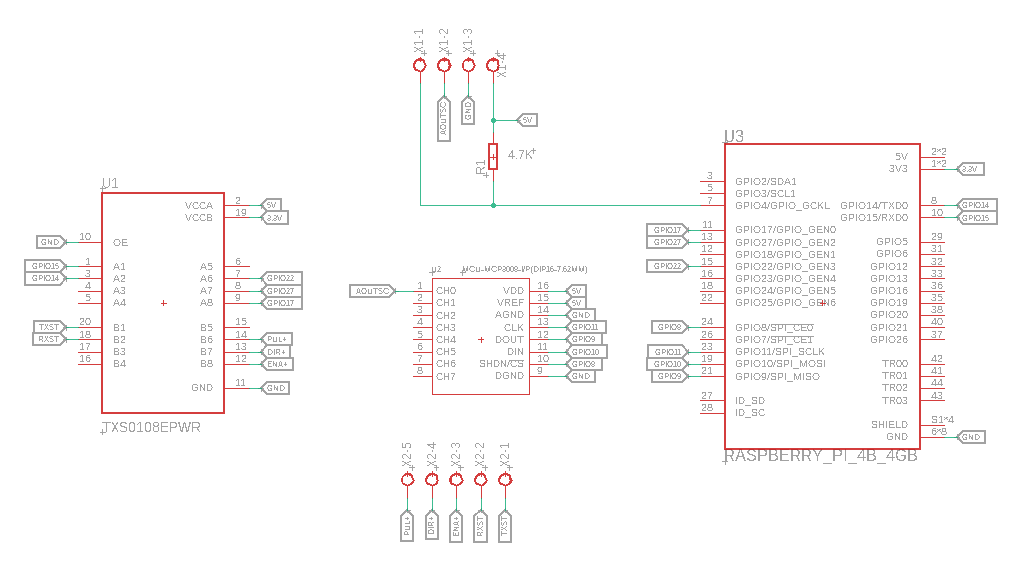
\includegraphics[width=0.92\linewidth,height=0.62\textheight,keepaspectratio]{./media/image97.png}
\captionof*{figure}{\small\itshape Figura 63. Esquemático Distribución 12V}
\addcontentsline{lof}{figure}{Figura 63. Esquemático Distribución 12V}
\label{fig:63}
\end{center}

\begin{center}
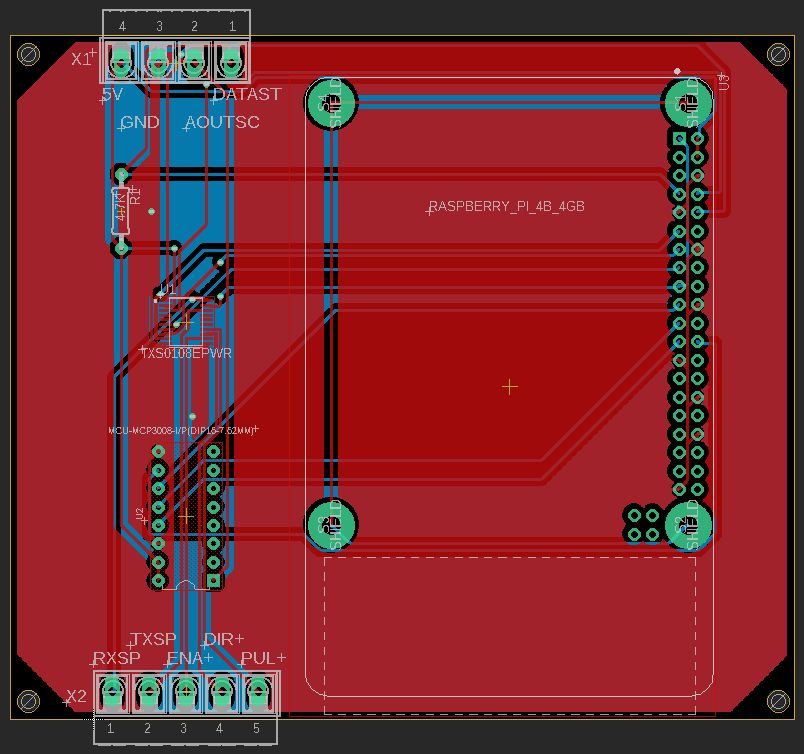
\includegraphics[width=0.92\linewidth,height=0.62\textheight,keepaspectratio]{./media/image11.png}
\captionof*{figure}{\small\itshape Figura 64. PCB Controlador Semafórico}
\addcontentsline{lof}{figure}{Figura 64. PCB Controlador Semafórico}
\label{fig:64}
\end{center}

\chapter{DISEÑO MECÁNICO DEL SISTEMA}\label{capuxedtulo-5-diseuxf1o-mecuxe1nico-del-sistema}

\section{Presentación general del sistema mecánico y requerimientos}\label{presentaciuxf3n-general-del-sistema-mecuxe1nico-y-requerimientos}

En este apartado se describen los componentes principales del sistema mecánico, su función dentro del proyecto y los requerimientos técnicos que guían el diseño, considerando criterios de resistencia, funcionalidad, mantenimiento y compatibilidad con el sistema electrónico y de control.

El sistema mecánico integra cuatro subsistemas principales: la estructura de protección exterior conformada por el gabinete de aluminio 5052-H32 con masa de 21.98 kg; el rack interno de soporte con masa de 5.700 kg que aloja todos los componentes electrónicos; el sistema de movimiento angular de la cámara con masa total de 3.5 kg que incluye motor paso a paso NEMA 23, biela y conector de aluminio 5052-H32, rodamiento de Ø120 mm, y aro estructural giratorio de 7.8 kg; y el conjunto de visión con cámara domo y soporte totalizando 0.65 kg. La masa total del sistema completo es de 47.126 kg, distribuida estratégicamente para optimizar estabilidad estructural y facilitar operaciones de instalación y mantenimiento.

El gabinete emplea aluminio 5052-H32 con espesor de 6 mm para cumplir protección mecánica IK10 requerida normativamente, proporcionando resistencia a tracción de 310 MPa y vida útil superior a lo requerido con acabado anodizado tipo II.

Explicaremos generalmente lo que se presenta en este capítulo apoyándonos del diseño del gabinete en su posición de centro de intersección vehicular visto en las figuras 65 y 66.

\begin{center}
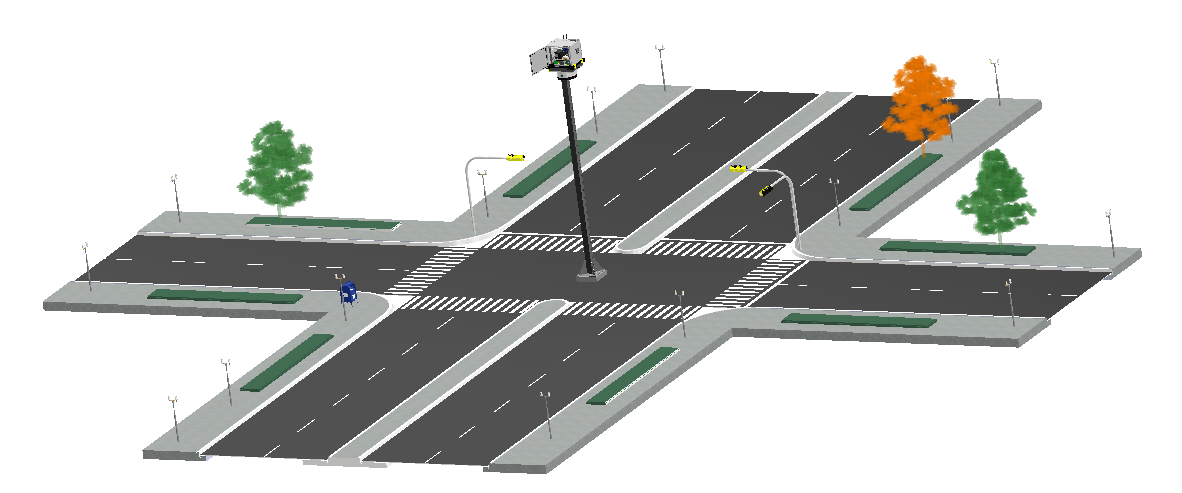
\includegraphics[width=0.92\linewidth,height=0.62\textheight,keepaspectratio]{./media/image30.png}
\captionof*{figure}{\small\itshape Figura 65. Vista del Controlador Semafórico en una intersección vehicular}
\addcontentsline{lof}{figure}{Figura 65. Vista del Controlador Semafórico en una intersección vehicular}
\label{fig:65}
\end{center}

\begin{center}
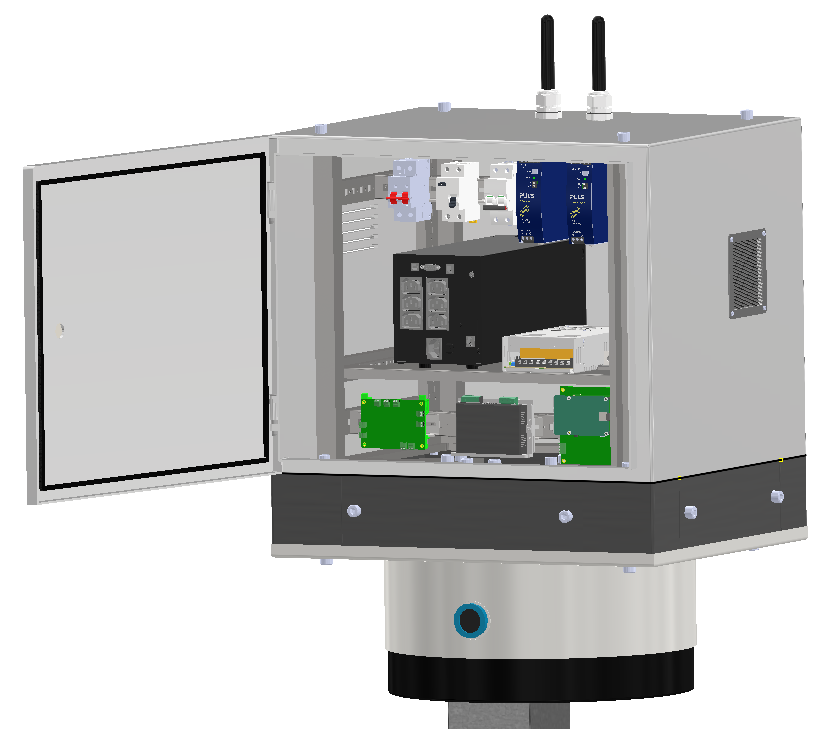
\includegraphics[width=0.92\linewidth,height=0.62\textheight,keepaspectratio]{./media/image64.png}
\captionof*{figure}{\small\itshape Figura 66. Vista del Controlador Semafórico}
\addcontentsline{lof}{figure}{Figura 66. Vista del Controlador Semafórico}
\label{fig:66}
\end{center}

\subsection{Requerimientos estructurales globales}\label{requerimientos-estructurales-globales}

El sistema de control adaptativo de tráfico debe soportar diversas cargas estructurales para garantizar su funcionalidad y seguridad operativa en diversas circunstancias. Cargas clasificadas en:

\textbf{Cargas muertas:} El sistema debe soportar el peso del gabinete y módulo IoT con sus componentes internos (placa, microcontrolador, sensores, actuadores y estructura), equipos como el UPS y el controlador, accesorios de comunicación (antenas y cámara) y cableado eléctrico y de comunicaciones (MML, 2022). Específicamente, el módulo debe soportar la cámara como sensor principal de detección vehicular, sistema de movimiento automatizado mediante actuador y componentes con peso total mostrado en la tabla 5.1.

\textbf{Cargas ambientales:} Las cargas de viento deben calcularse según AASHTO Standard Specifications, considerando tiempo de retorno de 50 años y velocidad de diseño correspondiente a Lima Metropolitana (MML, 2022).

Respecto a las cargas de temperatura, el documento de criterios municipales establece un rango operativo de -5°C a +60°C para equipamiento general y 0°C a 75°C para componentes específicos (MML, 2022). Sin embargo, el Manual ITS del MTC especifica que el módulo IoT debe ser resistente a altas temperaturas, humedad, polvo y exposición solar, operando en temperaturas extremas (MTC, 2020). Por su parte, la normativa de la Autoridad de Transporte Urbano (ATU) establece condiciones más restrictivas para equipos IoT con GPS, requiriendo temperatura de operación entre -20°C a +60°C y voltaje de operación de 8 a 32 VCC (ATU, 2024). Considerando el principio de adoptar el criterio más restrictivo, se establece el rango de -20°C a +60°C para garantizar cumplimiento normativo integral y operación en condiciones extremas.

\textbf{Requisitos de rigidez:} El sistema debe limitar deflexiones para evitar problemas de serviciabilidad bajo condiciones de carga muerta. El diseño debe considerar análisis de distribución de componentes, cálculo de centro de masa, análisis térmico para garantizar ventilación adecuada, y prueba de resistencia del gabinete evaluando zonas críticas de esfuerzo bajo cargas de vandalismo, humedad y vibraciones (MTC, 2020).

\textbf{Estabilidad estructural:} Se requiere resistencia a fatiga mediante diseño que considere efectos de cargas cíclicas de viento y deflexiones verticales por ráfagas de viento o tráfico, y dimensionamiento de estructuras según condiciones geotécnicas locales del suelo (MML, 2022).

\textbf{Protección contra corrosión:} Las estructuras metálicas requieren galvanización por inmersión en caliente con espesor mínimo de 1100 g/m\ensuremath{^{2}} según norma NTP-ISO 1461:2007, pintura de poliuretano o polisiloxano con resistencia UV, y tratamiento anticorrosivo en componentes expuestos (MML, 2022). Según el Manual ITS, el módulo debe ser resistente a la corrosión por exposición climática, considerando el clima de Lima (costa, alta humedad salina).

\textbf{Vida útil:} El sistema semafórico debe tener una vida útil mínima de 120 meses (10 años), las estructuras metálicas y gabinete del controlador mínimo 15 años, mientras que los equipos electrónicos sensibles tendrán vida útil garantizada mediante protección IP65/IK10 (MML, 2022).

\subsection{Restricciones de diseño}\label{restricciones-de-diseuxf1o}

Las dimensiones del gabinete de control semafórico han sido definidas en 800 mm \ensuremath{\times} 600 mm \ensuremath{\times} 500 mm (alto--ancho--profundidad), De acuerdo con las referencias técnicas internacionales, los gabinetes de control semafórico estándar definidos por la norma NEMA TS-2 / ITE ATC presentan dimensiones aproximadas de 1 245 mm \ensuremath{\times} 762 mm \ensuremath{\times} 432 mm, conocidas como formato ``M''. En este caso, el diseño propuesto conserva las proporciones funcionales y criterios de distribución interna de dichos modelos, pero con reducción volumétrica optimizada a los componentes presentes en su interior. Además, el sistema debe operar con humedad relativa hasta 90\%, resistir corrosión salina por proximidad al océano Pacífico, soportar exposición solar directa con radiación UV, y temperatura ambiente.

Se requiere grado de protección mínimo contra el ingreso de polvo y agua. Los criterios municipales establecen IP65 como mínimo (MML, 2022). Adicionalmente se requiere protección mecánica IK10 anti-vandálica, sistema de ventilación forzada activado a 40°C, y protección UV. Los dispositivos GPS deben contar con protección apropiada para condiciones de humedad y polución de Lima y Callao, con validación mediante pruebas en condiciones locales (ATU, 2024).

Se requiere transmisión en tiempo real con latencia máxima de 20 segundos, obligación de envío de información al Centro de Gestión y Monitoreo del SIT-ATU, y uso de API estandarizado desarrollado por ATU (ATU, 2024).

\subsection{Masa y Centro de masa del Sistema.}\label{masa-y-centro-de-masa-del-sistema.}

El análisis de masa y centro de gravedad del sistema es prioritario para garantizar la estabilidad estructural del gabinete y optimizar el diseño del sistema de anclaje al poste de soporte. Este apartado detalla el cálculo de las propiedades másicas de los tres componentes principales del sistema: el gabinete exterior, el rack interno con sus componentes electrónicos, y el sistema de cámara con su mecanismo de movimiento.

\begin{center}
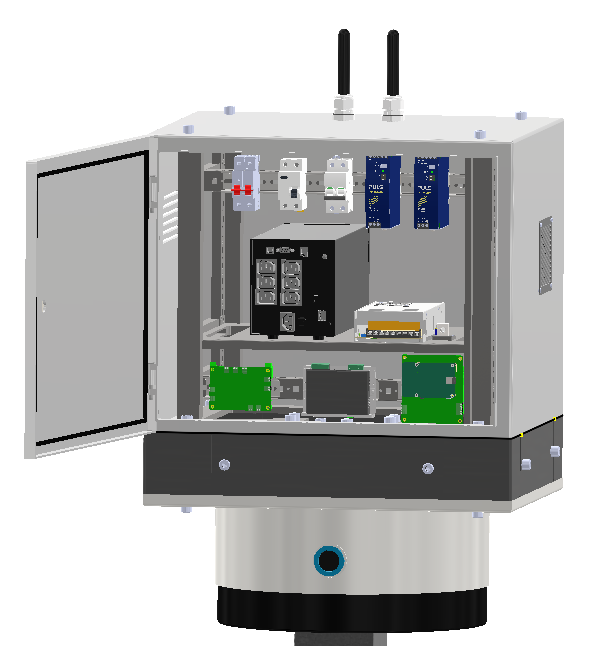
\includegraphics[width=0.92\linewidth,height=0.62\textheight,keepaspectratio]{./media/image111.png}
\captionof*{figure}{\small\itshape Figura 67. Sistema Completo, sin poste.}
\addcontentsline{lof}{figure}{Figura 67. Sistema Completo, sin poste.}
\label{fig:67}
\end{center}

Empezaremos el análisis con el gabinete protector de los componentes, este cuenta con la siguiente figura:

\begin{center}
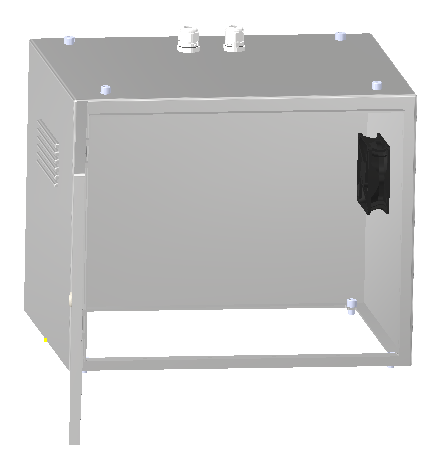
\includegraphics[width=0.92\linewidth,height=0.62\textheight,keepaspectratio]{./media/image109.png}
\captionof*{figure}{\small\itshape Figura 68. Gabinete Sin componentes.}
\addcontentsline{lof}{figure}{Figura 68. Gabinete Sin componentes.}
\label{fig:68}
\end{center}

El análisis de masa y centro de gravedad del sistema es prioritario para garantizar la estabilidad estructural del gabinete y optimizar el diseño del sistema de anclaje al poste de soporte. Este apartado detalla el cálculo de las propiedades másicas de los tres componentes principales del sistema: el gabinete exterior, el rack interno con sus componentes electrónicos, y el sistema de cámara con su mecanismo de movimiento.

El gabinete presenta una configuración geométrica de cubo hueco sin base inferior, tal como se observa en la Figura 66, con dimensiones exteriores de 479 mm de altura, 600 mm de ancho y 525 mm de profundidad lateral. La estructura está fabricada en aluminio 5052-H32, una aleación que combina resistencia estructural adecuada con bajo peso y excelente resistencia a la corrosión en ambientes salinos, característica crítica considerando la ubicación del sistema en Lima Metropolitana con proximidad al océano Pacífico. El espesor de pared seleccionado es de 6 mm, dimensión que proporciona rigidez suficiente para resistir cargas de viento y posibles impactos vandálicos, cumpliendo con el grado de protección mecánica IK10 requerido por la normativa municipal.

Para el cálculo de la masa del gabinete, se considera la densidad del aluminio 5052-H32 de 2680 kg/m\ensuremath{^{3}} según especificaciones del fabricante. El volumen de material se determina mediante la diferencia entre el volumen exterior total y el volumen interior hueco. El volumen exterior resulta de multiplicar las dimensiones externas:

\begin{centeredmath}
Volumen\ exterior = 0.479\ x\ 0.6\ x\ 0.525\  = \ 0.1509\ m\ensuremath{^{3}}\ \qquad (1)
\end{centeredmath}

Las dimensiones interiores se obtienen restando el doble del espesor de pared en ancho y profundidad, y un único espesor en altura debido a la ausencia de base inferior, resultando en 473 mm de altura interior, 588 mm de ancho interior y 513 mm de profundidad interior. El volumen interior calculado es:

\begin{centeredmath}
Volumen\ interior = 0.473\ x\ 0.588\ x\ 0.513\  = \ 0.1427\ m\ensuremath{^{3}}\ \qquad (2)
\end{centeredmath}

El volumen de material del gabinete se obtiene como:

\begin{centeredmath}
V_{Material} = 0.1509\  - 0.1427\  = \ 0.0082\ m\ensuremath{^{3}}\ \qquad (3)
\end{centeredmath}

La masa del gabinete, usando (3) y la densidad mencionada con anterioridad resulta:

\begin{centeredmath}
m_{gabinete} = 2680\ kg/m\ensuremath{^{3}}\ x\ 0.0082\  = \ 21.976\ \ kg\ \qquad (4)
\end{centeredmath}

El centro de masa del gabinete se determina considerando su geometría y la ausencia de la base inferior, factor que desplaza el centro de gravedad hacia arriba respecto al centro geométrico. En dirección horizontal (ancho), por simetría de la estructura, el centro de masa se ubica en el punto medio a 300 mm desde cualquier borde lateral. En dirección vertical (altura), la ausencia de la base inferior genera un desbalance másico que eleva el centro de gravedad aproximadamente a 250 mm desde la base, ligeramente por encima del centro geométrico que estaría a 239.5 mm. En dirección de profundidad, nuevamente por simetría, el centro se posiciona a 262.5 mm desde el borde frontal.

\begin{center}
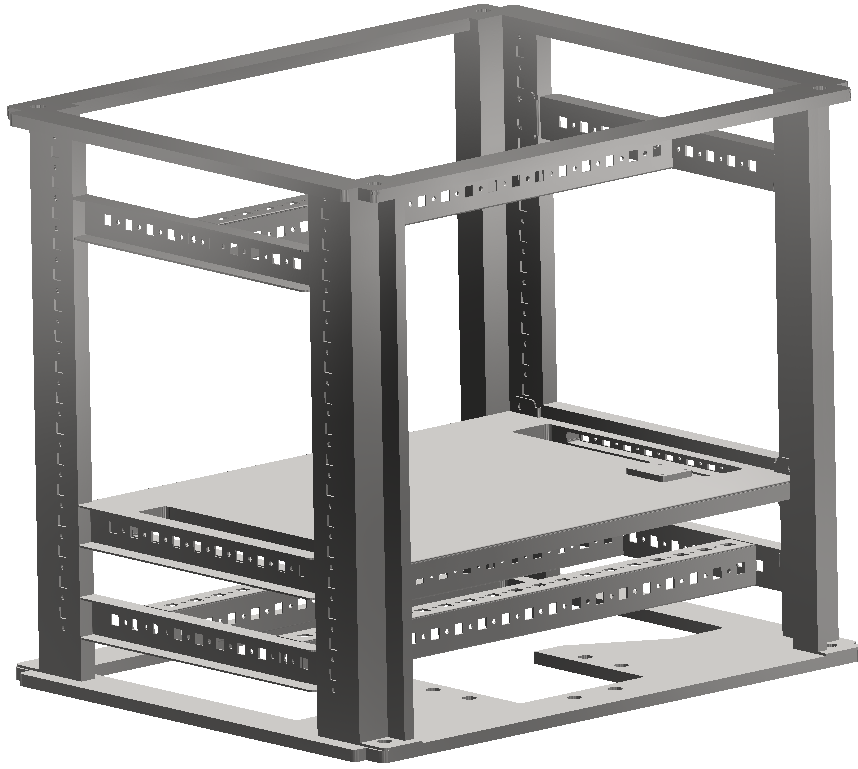
\includegraphics[width=0.92\linewidth,height=0.62\textheight,keepaspectratio]{./media/image145.png}
\captionof*{figure}{\small\itshape Figura 69. Rack Completo}
\addcontentsline{lof}{figure}{Figura 69. Rack Completo}
\label{fig:69}
\end{center}

El rack interno, representado en la Figura 67, constituye la estructura de soporte para todos los componentes electrónicos y de control del sistema. Sus dimensiones máximas son 466 mm de altura, 440 mm de ancho y 539 mm de profundidad lateral. La distribución vertical de componentes está optimizada para facilitar el mantenimiento, las conexiones eléctricas y la disipación térmica, siguiendo principios de diseño de sistemas embebidos industriales donde los componentes más pesados se ubican en niveles inferiores para reducir el centro de gravedad y mejorar la estabilidad.

En el nivel inferior del rack se encuentra un riel DIN que soporta los componentes de control y procesamiento: la Raspberry Pi 5 con su módulo HAT 4G LTE para comunicaciones celulares, el driver DM542T del motor paso a paso que controla el sistema de movimiento de la cámara, y la PCB de distribución que gestiona el ruteo de alimentación y señales. Este nivel está posicionado ligeramente hacia el frente del rack, es decir hacia la puerta del gabinete, facilitando el acceso durante operaciones de mantenimiento sin necesidad de desmontar componentes superiores. Como se observa en las siguientes Figuras:

\begin{center}
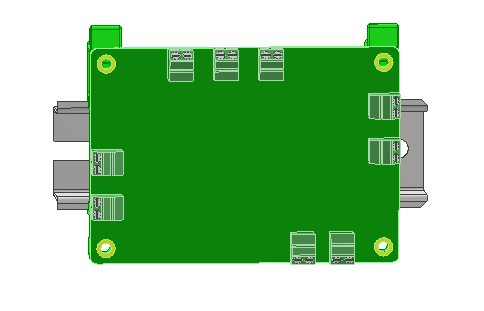
\includegraphics[width=0.92\linewidth,height=0.62\textheight,keepaspectratio]{./media/image84.png}
\captionof*{figure}{\small\itshape Figura 70. PCB Distribuidor de Voltaje}
\addcontentsline{lof}{figure}{Figura 70. PCB Distribuidor de Voltaje}
\label{fig:70}
\end{center}

\begin{center}
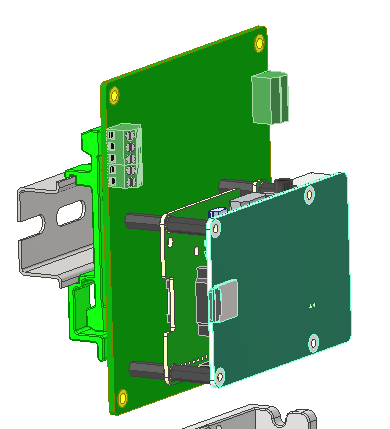
\includegraphics[width=0.92\linewidth,height=0.62\textheight,keepaspectratio]{./media/image70.png}
\captionof*{figure}{\small\itshape Figura 71. PCB Controlador Semafórico - Raspberry con HAT}
\addcontentsline{lof}{figure}{Figura 71. PCB Controlador Semafórico - Raspberry con HAT}
\label{fig:71}
\end{center}

\begin{center}
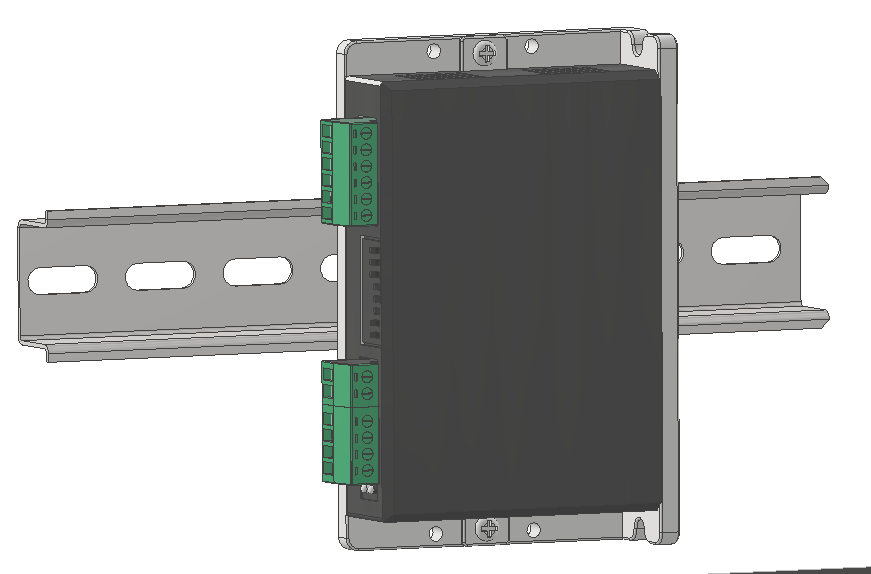
\includegraphics[width=0.92\linewidth,height=0.62\textheight,keepaspectratio]{./media/image14.png}
\captionof*{figure}{\small\itshape Figura 72. Driver de Motor Pap 23}
\addcontentsline{lof}{figure}{Figura 72. Driver de Motor Pap 23}
\label{fig:72}
\end{center}

El nivel superior del rack presenta una configuración dual con una base de soporte horizontal que ocupa toda el área disponible, sobre la cual se montan los dos componentes más pesados del sistema: el UPS que garantiza continuidad operativa ante cortes de suministro eléctrico, y la fuente de alimentación conmutada SMPS modelo S-360-24 que proporciona los 24V DC estabilizados para el sistema. Esta ubicación intermedia de los elementos pesados podría parecer contradictoria con el principio de centro de gravedad bajo, sin embargo, está justificada por consideraciones térmicas ya que estos componentes generan calor significativo durante su operación y requieren proximidad a las rejillas de ventilación superior del gabinete. Componentes observados en la Figura 73

\begin{center}
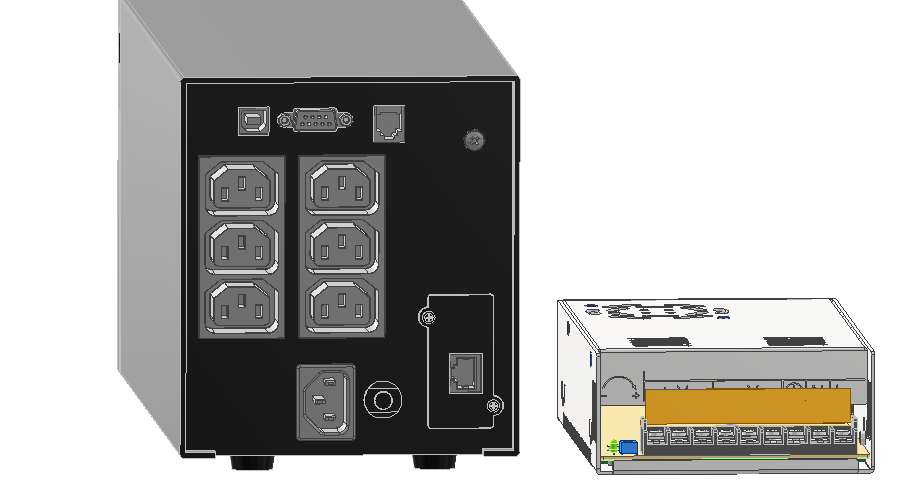
\includegraphics[width=0.92\linewidth,height=0.62\textheight,keepaspectratio]{./media/image57.png}
\captionof*{figure}{\small\itshape Figura 73. UPS y SMPS}
\addcontentsline{lof}{figure}{Figura 73. UPS y SMPS}
\label{fig:73}
\end{center}

Por encima del mencionado, otro riel DIN aloja los dispositivos de protección eléctrica y conversión de voltaje. El breaker termomagnético Schneider C60N-C 6 de 18 mm de ancho proporciona protección contra sobrecorrientes, el dispositivo diferencial residual (RCD) Schneider ID K con capacidad de 25A y sensibilidad de 30mA protege contra fugas a tierra, el dispositivo de protección contra sobretensiones (DPS) Phoenix Contact VAL-MS 230 de 18 mm salvaguarda el sistema de transientes de red, y dos conversores DC-DC basados en el regulador LM2596 proporcionan los voltajes secundarios de 5V y 12V requeridos por diferentes subsistemas. Observado en la figura 74.

\begin{center}
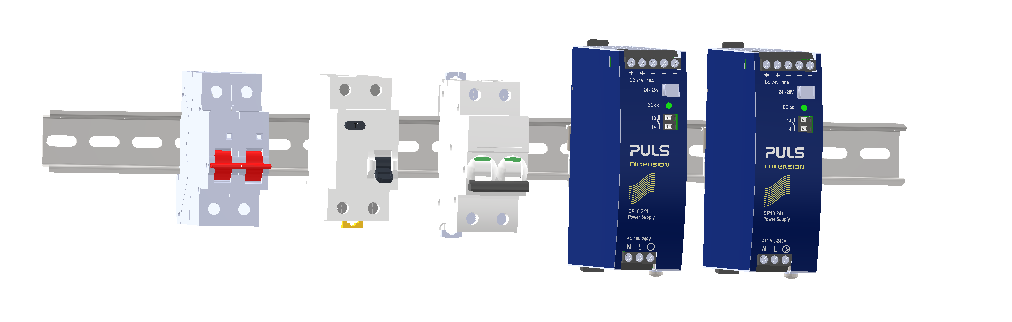
\includegraphics[width=0.92\linewidth,height=0.62\textheight,keepaspectratio]{./media/image79.png}
\captionof*{figure}{\small\itshape Figura 74. Componentes de protección y DC DC}
\addcontentsline{lof}{figure}{Figura 74. Componentes de protección y DC DC}
\label{fig:74}
\end{center}

La masa de cada componente se obtiene de las especificaciones técnicas de los fabricantes. La Raspberry Pi 5 tiene una masa de 0.075 kg según especificaciones oficiales de Raspberry Pi Foundation. El módulo HAT 4G LTE con el módem Quectel EG25-G pesa 0.050 kg. El driver de motor paso a paso DM542T, que incluye disipador térmico de aluminio extruido, tiene una masa de 0.350 kg. La PCB de distribución, diseñada específicamente para este proyecto con dimensiones de 100 \ensuremath{\times} 70 mm y sustrato FR-4 de 1.6 mm, se estima en 0.300 kg considerando el peso del cobre, componentes montados y conectores.

El UPS seleccionado, con capacidad nominal de 500VA para proporcionar respaldo durante cortes breves de suministro, presenta una masa de 3.500 kg que incluye las baterías de plomo-ácido selladas tipo VRLA. La fuente de alimentación conmutada SMPS S-360-24 con potencia nominal de 360W pesa 1.200 kg según ficha técnica del fabricante. Los dispositivos de protección eléctrica tienen masas individuales de 0.100 kg para el breaker C60N-C6, 0.150 kg para el RCD ID K, y 0.080 kg para el DPS VAL-MS 230, todas obtenidas de catálogos de Schneider Electric y Phoenix Contact. Los conversores DC-DC basados en LM2596 tienen cada uno una masa aproximada de 0.040 kg.

La estructura del rack fabricada en aluminio con perfiles de 30\ensuremath{\times}30 mm y bandejas perforadas se estima en 5.700 kg mediante cálculo volumétrico considerando el volumen de los perfiles estructurales y las bandejas de soporte. El cableado interno que incluye cables de potencia, señal y comunicaciones junto con conectores y terminales tiene una masa de 0.400 kg. Las antenas de comunicación celular y conectores externos suman 0.300 kg. El sistema de gestión térmica incluye un ventilador axial de 120 \ensuremath{\times} 120 \ensuremath{\times} 38 mm operando a 24V DC con masa de 0.200 kg. Sumando todas estas contribuciones, la masa total del rack con componentes electrónicos y accesorios resulta en 11.965 kg.

El centro de masa del rack no se encuentra en su centro geométrico debido a la distribución asimétrica de componentes. La concentración de masa en la zona frontal (Raspberry Pi, driver, PCB de distribución) y la ubicación del UPS y SMPS en la base desplazan el centro de gravedad hacia el frente y hacia abajo. Considerando los momentos másicos de cada componente respecto a un sistema de coordenadas con origen en la esquina inferior posterior del rack, se estima que el centro de masa se ubica aproximadamente a 220 mm desde el borde posterior (frontal del rack hacia la puerta), a 180 mm desde la base (zona inferior donde están los componentes pesados), y a 250 mm lateralmente respecto al centro del ancho.

\begin{center}
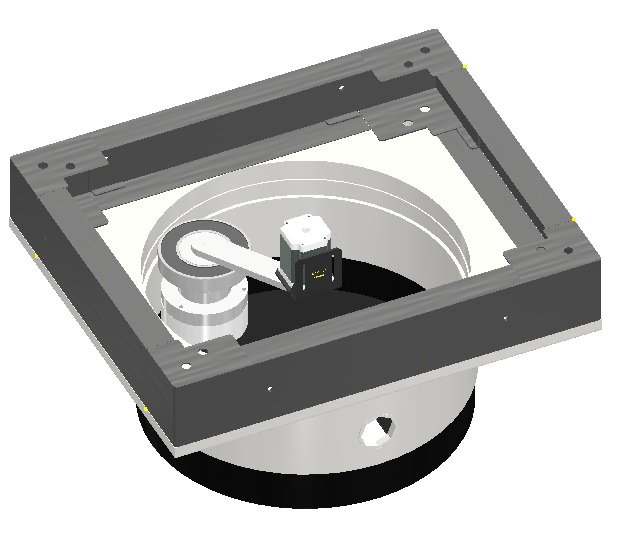
\includegraphics[width=0.92\linewidth,height=0.62\textheight,keepaspectratio]{./media/image16.png}
\captionof*{figure}{\small\itshape Figura 75. Sistema de Vigilancia}
\addcontentsline{lof}{figure}{Figura 75. Sistema de Vigilancia}
\label{fig:75}
\end{center}

La transmisión mecánica está constituida por una biela de aluminio con dimensiones de 150 \ensuremath{\times} 35 \ensuremath{\times} 10 mm y masa de 0.142 kg. El acoplamiento entre la cámara y la biela se realiza mediante un conector de aluminio con geometría cilíndrica de diámetro exterior máximo Ø111 mm, pasante central Ø65 mm y altura total de 55.5 mm, resultando en una masa de 0.857 kg. El elemento de rotación es un rodamiento rígido de bolas de Ø120 mm con masa de 1.000 kg, montado sobre un aro estructural de aluminio 5052-H32 de 7.800 kg que constituye la base del sistema de visión. Este aro incluye en su parte inferior un protector circular plano de policarbonato con diámetro Ø420 mm y espesor de 2 mm, proporcionando protección mecánica y ambiental al sistema con una masa de 1.000 kg. El actuador del sistema es un motor paso a paso NEMA 23 con torque nominal de 1.8 N·m y masa de 1.500 kg según especificaciones del fabricante.

El anodizado tipo II de 10-25 \ensuremath{\mu}m de espesor que se aplicará como acabado superficial incrementa la resistencia a la corrosión y proporciona una superficie resistente al desgaste, garantizando vida útil superior a 10 años en servicio exterior continuo. El sistema de control y procesamiento está conformado por dos PCBs principales: la PCB controladora que integra la Raspberry Pi 5 (0.075 kg) y el módulo HAT 4G LTE con módem Quectel EG25-G (0.050 kg) montados sobre una placa base de circuito impreso FR-4 de 1.6 mm (0.050 kg), resultando en un conjunto de 0.175 kg; y la PCB de distribución de voltaje con masa de 0.300 kg que gestiona el ruteo de alimentación hacia todos los subsistemas. La instrumentación de monitoreo distribuida incluye tres sensores específicos: sensor de corriente WCS1600 con masa de 0.015 kg para supervisión del consumo energético del sistema, sensor ultrasónico URM06 con interfaz RS485 y masa de 0.025 kg para detección de proximidad y verificación de objetos, y sensor de temperatura DS18B20 con sonda y masa de 0.020 kg para monitoreo térmico continuo del gabinete y activación del sistema de ventilación forzada. El conjunto de elementos de fijación mecánica está clasificado según su función estructural: 8 tornillos M24 con masa total de 1.440 kg para la conexión crítica en el poste, garantizando transmisión adecuada de cargas gravitatorias y momentos de vuelco; 30 tornillos M12 con masa de 1.050 kg para montaje de componentes en el rack y el gabinete. Además de servir en la fijación de bandejas y 8 tornillos M3 con masa de 0.016 kg para fijación de las placas de circuito impreso sobre los rieles DIN y conectar el sensor de corriente y el motor Pap a su respectivo soporte.

El sistema de adquisición visual está constituido por una cámara domo con masa de 0.600 kg montada sobre un soporte de aluminio de 0.050 kg, totalizando 0.650 kg para el conjunto de visión. Esta cámara se posiciona en la parte móvil del sistema, permitiendo desplazamiento angular de 180° sobre el aro giratorio para optimizar el campo de visión según las necesidades de monitoreo del tráfico vehicular. Esta ubicación inferior es estratégica porque reduce el momento de vuelco del conjunto gabinete-poste ante cargas laterales de viento y minimiza la longitud de cableado de datos y alimentación desde el rack interno. La influencia del conjunto de visión en el centro de masa global del sistema es limitada debido a dos factores principales. Primero, su masa de 0.650 kg representa el 1.38\% de la masa total del sistema que es de 47.126 kg, por lo que su contribución al momento másico es proporcionalmente pequeña. Segundo, su posición cercana al punto de apoyo del poste de soporte minimiza el brazo de palanca respecto al eje de rotación potencial del sistema, reduciendo aún más su efecto en el equilibrio general. Por estas razones, en cálculos preliminares de estabilidad estructural, la influencia del sistema de visión puede considerarse despreciable sin introducir un error significativo en los resultados.

La masa total del sistema se obtiene sumando las contribuciones de todos los componentes principales y elementos accesorios:

\begin{centeredmath}
m_{total} = m_{gabinete}\  + \ m_{rack}\  + m_{aro}\ {+ m}_{sistema\ movimiento}\  + \ m_{accesorios} = \ 47.126\ kg\ \qquad (1)
\end{centeredmath}

La masa total del sistema completo resulta en 47.126 kg, aproximadamente 47.1 kg. Los datos específicos de cada componente se presentan en la tabla de anexos.

El centro de masa global del sistema completo se determina mediante el principio de momentos másicos, ponderando la posición de cada componente por su masa relativa. Definiendo un sistema de coordenadas con origen en la esquina inferior posterior izquierda del gabinete, con eje X positivo hacia el frente (dirección de la puerta), eje Y positivo hacia arriba, y eje Z positivo hacia la derecha vista desde el frente, se calculan las coordenadas del centro de masa global.

En dirección X (frontal), el centro de masa del gabinete se ubica a 300 mm (centro geométrico), el del rack a 220 mm (desplazado hacia el frente), y el de la cámara a 300 mm. Aplicando la fórmula de centro de masa ponderado:

\begin{centeredmath}
X_{cm} = (m_{gabinete}\ x\ X_{gabinete\ } + \ m_{rack}\ x\ X_{rack}\ \ {+ m}_{\text{cámara}}\ x\ X_{\text{cámara}})/m_{total} = \ 273.2\ mm\ 
\end{centeredmath}

\hl{En dirección Y (vertical), considerando que el centro del gabinete está a 250 mm, el del rack a 180 mm, y el de la cámara a 100 mm desde la base:}

\begin{centeredmath}
Y_{cm} = (m_{gabinete}\ x\ Y_{gabinete\ } + \ m_{rack}\ x\ Y_{rack}\ \ {+ m}_{\text{cámara}}\ x\ Y_{\text{cámara}})/m_{total} = \ 223.9\ mm\ 
\end{centeredmath}

\hl{En dirección Z (lateral), siendo las posiciones 262.5 mm para el gabinete, 250 mm para el rack, y 262.5 mm para la cámara:}

\begin{centeredmath}
Z_{cm} = (m_{gabinete}\ x\ Z_{gabinete\ } + \ m_{rack}\ x\ Z_{rack}\ \ {+ m}_{\text{cámara}}\ x\ Z_{\text{cámara}})/m_{total} = \ 254.9\ mm\ 
\end{centeredmath}

\hl{El centro de masa global del sistema se encuentra por tanto en las coordenadas (273.2 mm, 223.9 mm, 254.9 mm), lo que indica una posición ligeramente desplazada hacia el frente del gabinete debido a la concentración de componentes electrónicos en esa zona, ubicada por debajo del centro vertical debido al peso significativo del UPS y SMPS en la parte inferior, y prácticamente centrada en dirección lateral debido a la simetría del diseño en ese eje.}

\hl{Esta ubicación del centro de masa justifica la decisión de diseño de posicionar el punto de apoyo del poste de soporte a 110 mm desde el frente del gabinete, ligeramente por debajo del centro vertical. Esta posición del punto de anclaje minimiza los momentos de vuelco ante cargas laterales de viento, reduce las tensiones en las uniones soldadas entre gabinete y poste, y facilita el paso de cables de alimentación y comunicación desde el poste hacia el interior del gabinete sin crear interferencias mecánicas con los componentes internos. Además, esta configuración permite que el poste de soporte, fabricado en acero estructural con sección transversal cuadrada, trabaje predominantemente a compresión bajo cargas verticales gravitatorias, optimizando la eficiencia estructural del conjunto.}

\hl{Datos específicos en la tabla de anexos.}

\subsection{Criterios de selección de materiales}\label{criterios-de-selecciuxf3n-de-materiales}

La selección de materiales para el sistema de control adaptativo inteligente se fundamenta en el cumplimiento de requisitos normativos nacionales e internacionales, las condiciones ambientales extremas de Lima Metropolitana, y la necesidad de garantizar durabilidad, seguridad y compatibilidad con la infraestructura semafórica existente.

\textbf{Materiales estructurales del gabinete}

Se selecciona aleación de aluminio 5052-H32 para la fabricación del gabinete del módulo IoT, con dimensiones de 600 mm \ensuremath{\times} 500 mm \ensuremath{\times} 600 mm. Esta aleación se utiliza en entornos exteriores e industriales debido a su alta resistencia a la corrosión en atmósferas marinas y urbanas, su buena soldabilidad y su excelente conformabilidad, lo que permite un proceso de manufactura eficiente (Atlas, 2021; ThomasNet, 2025).

Aunque la norma NEMA TS-2 (Traffic Controller Assemblies) establece los requisitos funcionales, ambientales y estructurales para gabinetes de control de tráfico, no impone un material específico para su construcción (NEMA, 2021). Por ello, el uso de aluminio 5052-H32 no constituye un requisito normativo, pero sí representa una elección adecuada para cumplir los niveles de desempeño exigidos por NEMA TS-2 y el grado de protección IP65, garantizando estanqueidad y durabilidad en ambientes de alta humedad salina como Lima y Callao.

La aleación 5052-H32 (temple H32 = endurecido por deformación y parcialmente estabilizado) contiene 2.2--2.8 \% de magnesio y 0.15--0.35 \% de cromo, elementos que mejoran notablemente su resistencia a la corrosión general y por picaduras, especialmente en ambientes marinos.

Gracias a esta composición, el aluminio 5052-H32 se considera de grado marino, adecuado para estructuras expuestas a la intemperie y atmósferas salinas.

\textbf{Ventajas comparativas del material seleccionado}

En comparación con el acero galvanizado, la aleación de aluminio 5052-H32 presenta ventajas técnicas y operativas como:

\begin{itemize}
\item
  Reducción de peso de aproximadamente 65 \%, lo que facilita la instalación, disminuye esfuerzos sobre la estructura de soporte y permite maniobras más seguras durante el mantenimiento (Atlas, 2021).
\item
  Alta resistencia a la corrosión salina, lograda por su contenido de magnesio (2.2 - 2.8 \%), que protege frente a la oxidación sin requerir procesos de galvanización.
\item
  Alta conductividad térmica (138 W/m·K), lo que favorece la disipación eficiente del calor generado por los componentes electrónicos internos, prolongando su vida útil (MatWeb, 2024).
\end{itemize}

Por otro lado, frente al policarbonato reforzado, también utilizado en ciertos gabinetes de control semafórico, el aluminio 5052-H32 ofrece beneficios adicionales:

\begin{itemize}
\item
  Mayor resistencia mecánica y rigidez estructural, especialmente ante impactos o vibraciones.
\item
  Mejor capacidad de disipación térmica, fundamental para alojar fuentes, controladores y módulos de potencia sin riesgo de sobrecalentamiento.
\item
  Mayor durabilidad ante exposición prolongada a radiación UV, con una vida útil estimada superior a 15 años, frente a los 12 años del policarbonato reforzado en exteriores (Wevolver, 2025).
\item
  Facilidad de conexión a tierra eléctrica, lo que mejora la protección contra descargas atmosféricas o transitorias en el sistema electrónico.
\end{itemize}

\section{Diseño del sistema de movimiento para la cámara}\label{diseuxf1o-del-sistema-de-movimiento-para-la-cuxe1mara}

El sistema de posicionamiento angular de la cámara permite un desplazamiento de 180° mediante un mecanismo de biela-manivela acoplado a un rodamiento rígido de bolas. El diseño busca maximizar la estabilidad y minimizar vibraciones que puedan afectar la calidad de captura de imágenes.

El mecanismo consiste en una biela de 150 mm conectada al eje del motor paso a paso NEMA 23, que transmite movimiento a la pista interior de un rodamiento de 120 mm de diámetro exterior. La cámara domo y su soporte se montan sobre esta pista móvil, permitiendo el desplazamiento controlado a lo largo del arco. El rodamiento cumple función dual de soporte estructural y reductor de fricción, con la pista exterior fija mediante un aro estructural con dos puntos de apoyo diametralmente opuestos.

La configuración de apoyo bilateral distribuye el peso del conjunto cámara-soporte (210 gramos) entre dos puntos, eliminando prácticamente la necesidad de que el motor genere torque para soportar cargas gravitatorias. La potencia del motor se destina exclusivamente a vencer fricción residual en el rodamiento y fuerzas inerciales durante aceleración y desaceleración angular. Observable el sistema en la figura 76, 77 y 78.

\begin{center}
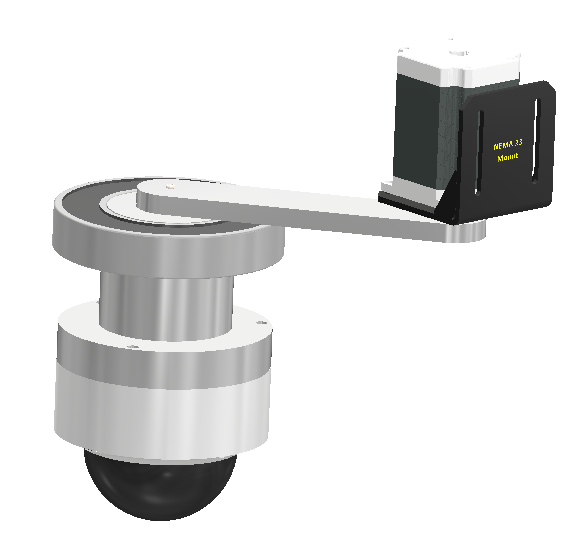
\includegraphics[width=0.92\linewidth,height=0.62\textheight,keepaspectratio]{./media/image42.png}
\captionof*{figure}{\small\itshape Figura 76. Camara - Soporte y Biela}
\addcontentsline{lof}{figure}{Figura 76. Camara - Soporte y Biela}
\label{fig:76}
\end{center}

\begin{center}
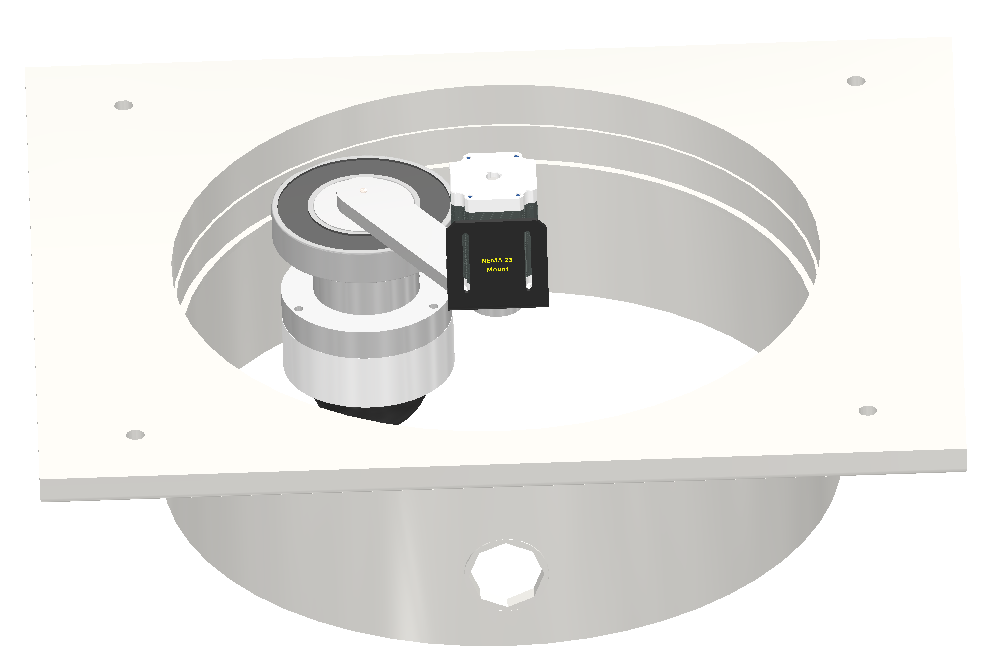
\includegraphics[width=0.92\linewidth,height=0.62\textheight,keepaspectratio]{./media/image37.png}
\captionof*{figure}{\small\itshape Figura 77. Vista del Aro de giro y el rodamiento}
\addcontentsline{lof}{figure}{Figura 77. Vista del Aro de giro y el rodamiento}
\label{fig:77}
\end{center}

\begin{center}
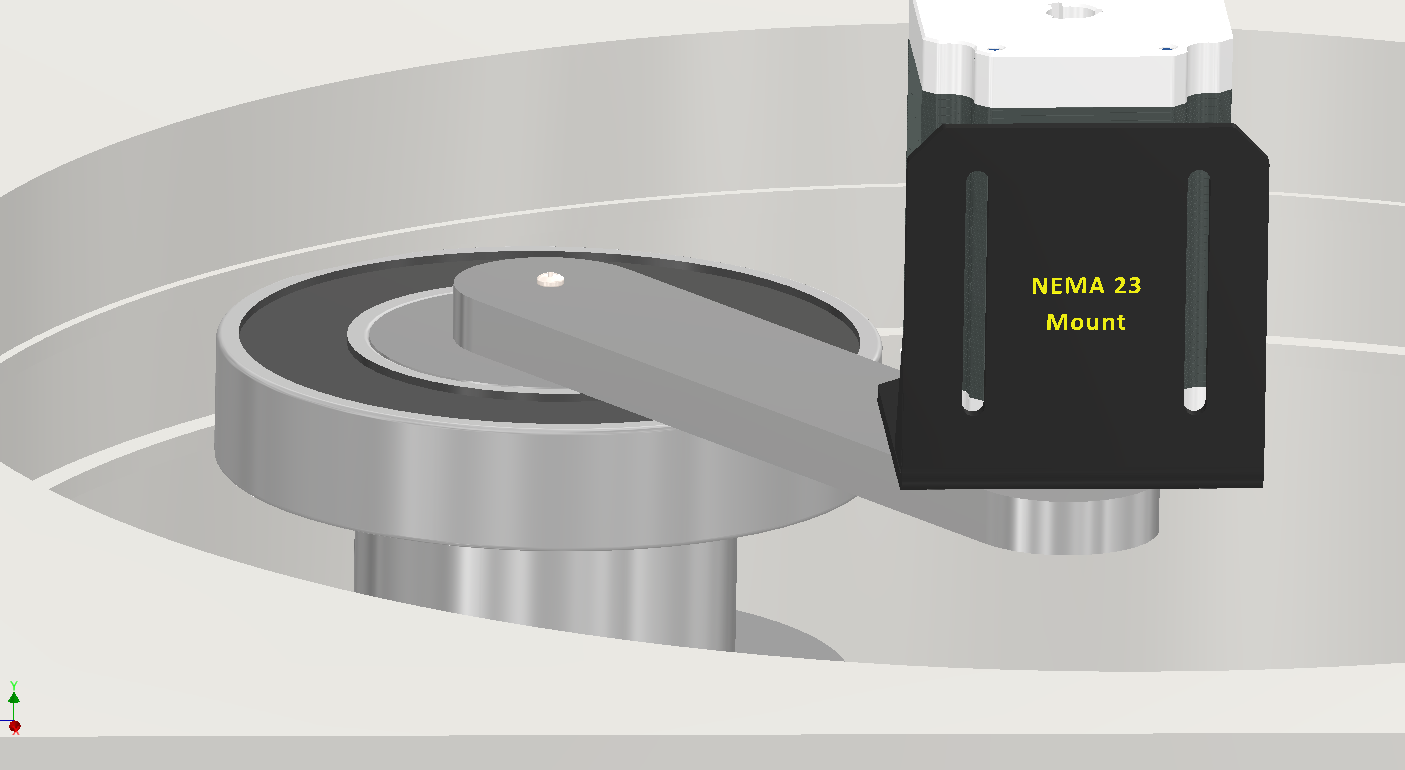
\includegraphics[width=0.92\linewidth,height=0.62\textheight,keepaspectratio]{./media/image51.png}
\captionof*{figure}{\small\itshape Figura 78. Vista del rodamiento, biela y motor}
\addcontentsline{lof}{figure}{Figura 78. Vista del rodamiento, biela y motor}
\label{fig:78}
\end{center}

\subsection{Cálculos estructurales}\label{cuxe1lculos-estructurales}

Determinación de los esfuerzos, momentos y deformaciones bajo condiciones de operación y carga. Empezaremos con los datos relevantes de los componentes.

Primero se realizará el análisis del diagrama de cuerpo libre (DCL) del sistema de vigilancia mostrado en la Figura 79. El DCL representa todas las fuerzas actuantes sobre cada componente del sistema de movimiento angular de la cámara, donde:

\begin{itemize}
\item
  \textbf{Wm}: Peso del motor PAP NEMA 23
\item
  \textbf{Wb}: Peso de la biela de transmisión
\item
  \textbf{Wa}: Peso del aro estructural giratorio
\item
  \textbf{Ws}: Peso del soporte de cámara
\item
  \textbf{Wc}: Peso de la cámara domo
\item
  \textbf{Wr}: Peso del rodamiento de Ø120 mm
\item
  \textbf{Gx, Gy}: Reacciones en la sujeción con el gabinete superior
\item
  \textbf{B}: Fuerza normal transmitida por la biela
\item
  \textbf{N, Ns}: Fuerzas normales de reacción en rodamiento y soporte
\item
  \textbf{NC1, NC2}: Fuerzas normales en los puntos de contacto de la cámara con el soporte
\item
  \textbf{FR}: Fuerzas de fricción en el rodamiento
\item
  \textbf{T}: Torque transmitido por el motor
\end{itemize}

El sistema de movimiento se basa en un mecanismo de biela-manivela que transmite movimiento rotacional del motor hacia movimiento angular de la cámara a través del rodamiento, con el aro estructural proporcionando soporte y guiado del desplazamiento.

\begin{center}
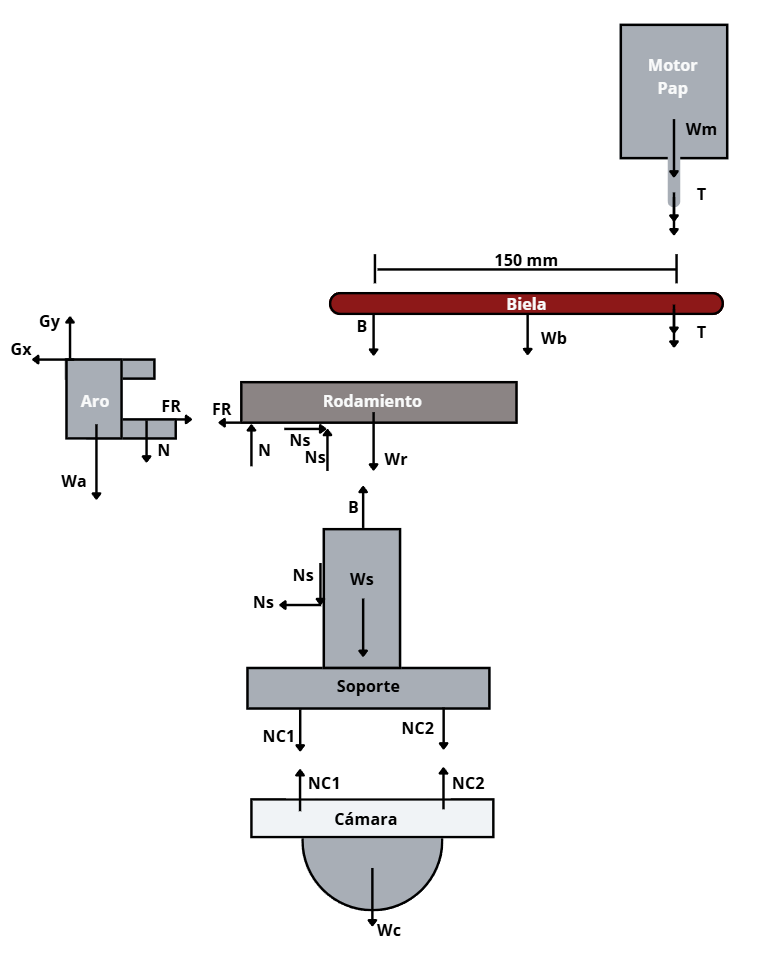
\includegraphics[width=0.92\linewidth,height=0.62\textheight,keepaspectratio]{./media/image125.png}
\captionof*{figure}{\small\itshape Figura 79. DCL del sistema de vigilancia}
\addcontentsline{lof}{figure}{Figura 79. DCL del sistema de vigilancia}
\label{fig:79}
\end{center}

\textbf{Rodamiento:}

• Diámetro exterior (D): 120 mm

• Radio medio de trabajo (r): 60 mm

• Tipo: Rodamiento rígido de bolas sellado con grasa

• Coeficiente de fricción (\ensuremath{\mu}): 0.002

\textbf{Biela de transmisión:}

• Longitud entre centros (L): 150 mm

• Ancho (b): 35 mm

• Espesor (e): 10 mm

• Material: Aluminio 5052-H32

• Área transversal (A): 350 mm\ensuremath{^{2}}

\textbf{Conector cámara-biela:}

\begin{itemize}
\item
  Material: Aluminio 5052-H32
\item
  Masa: 0.857 kg
\item
  Fabricación: Mecanizado CNC
\end{itemize}

\textbf{Aro estructural:}

\begin{itemize}
\item
  Material: Aluminio 5052-H32
\item
  Masa: 7.800 kg
\end{itemize}

\textbf{Conjunto cámara y soporte:}

\begin{itemize}
\item
  Masa de cámara domo: m\ensuremath{_{1}} = 0.600 kg
\item
  Masa de soporte (Aluminio 5052-H32): m\ensuremath{_{2}} = 0.050 kg
\item
  Masa total conjunto visión: mtotal = 0.650 kg
\item
  Peso nominal: Wc + Ws = 0.650 \ensuremath{\times} 9.81 = 6.38 N
\end{itemize}

\textbf{Motor Nema 23:}

\begin{itemize}
\item
  Torque nominal: 1.8 N·m
\item
  Masa: 1.500 kg
\end{itemize}

El aro estructural soporta el peso del rodamiento (Wr), parte del sistema de cámara, y las reacciones provenientes de la biela. Las reacciones en los puntos de sujeción con el gabinete (Gx, Gy) deben equilibrar todas estas cargas.

Equilibrio vertical:

\begin{centeredmath}
\Sigma Fy\  = \ 0:\ Gy\  - \ Wa\  - \ Wr\  - \ Ws\  - \ Wc\  - \ componente\ vertical\ de\ B\  = \ 0\ \ \qquad (1)
\end{centeredmath}

\begin{centeredmath}
Gy\  = \ 76.52\  + \ 9.81\  + \ 0.49\  + \ 5.89\  + \ B \cdot sen(\theta)\ \ \ \qquad (2)
\end{centeredmath}

\begin{centeredmath}
Gy\  \approx \ 92.71\ N\  + \ B \cdot sen(\theta)\ \ \ \qquad (3)
\end{centeredmath}

Donde \ensuremath{\theta} es el ángulo instantáneo de la biela respecto a la horizontal.

Equilibrio horizontal:

\begin{centeredmath}
\Sigma Fx\  = \ 0:\ Gx\  - \ FR\  - \ componente\ horizontal\ de\ B\  = \ 0\ \ \qquad (4)
\end{centeredmath}

\begin{centeredmath}
Gx\  = \ FR\  + \ B \cdot cos(\theta)\ (2)\ \ \ \qquad (5)
\end{centeredmath}

La cámara se apoya sobre el soporte mediante dos puntos de contacto (NC1, NC2). El equilibrio vertical requiere:

\begin{centeredmath}
\Sigma Fy\  = \ 0:\ NC1\  + \ NC2\  - \ Wc\  - \ Ws\  = \ 0\ \ \qquad (6)
\end{centeredmath}

\begin{centeredmath}
\ \ \ \ \ \ \ \ \ \ \ \ \ \ \ \ \ \ \ \ \ \ \ \ \ \ \ \ \ \ \ \ \ \ \ \ \ \ \ \ \ \ \ \ \ \ \ \ \ NC1\  + \ NC2\  = \ 5.89\  + \ 0.49\  = \ 6.38\ N\qquad (7)
\end{centeredmath}

Asumiendo distribución uniforme por simetría:

NC1 = NC2 = 3.19 N

Fuerzas de fricción en el rodamiento

La fuerza de fricción en el rodamiento se opone al movimiento rotacional y depende de la carga normal total sobre el rodamiento (que incluye el peso del aro, rodamiento, soporte y cámara):

Carga normal en rodamiento = Wa + Wr + Ws + Wc = 92.71 N (8)

Fuerza de fricción:

FR = \ensuremath{\mu} \ensuremath{\times} Carga normal = 0.002 \ensuremath{\times} 92.71 = 0.185 N (9)

Esta fuerza de fricción genera un torque resistivo en el eje del rodamiento:

Tfricción = FR \ensuremath{\times} r = 0.185 N \ensuremath{\times} 0.060 m = 0.011 N·m = 11 mN·m (10)

\subsection{Análisis de Cargas y Requerimientos de Torque}\label{anuxe1lisis-de-cargas-y-requerimientos-de-torque}

El motor debe vencer dos componentes de resistencia: la fricción en el rodamiento y las fuerzas inerciales durante la aceleración angular. Se adopta un factor de seguridad FS = 2.0 para dimensionamiento, estándar en maquinaria ligera con cargas dinámicas moderadas.

\begin{centeredmath}
W_{\text{diseño}}\  = \ FS\  \times \ (Ws + Wc)\  = \ 2.0\  \times \ 6.38\ N\  = \ 12.76\ N\ \ \qquad (1)
\end{centeredmath}

Los rodamientos rígidos de bolas lubricados presentan coeficientes de fricción excepcionalmente bajos (\ensuremath{\mu} = 0.002) debido al contacto de tipo rodadura pura entre pistas y elementos rodantes.

\begin{centeredmath}
T_{\text{fricción}}\  = \ \mu_{\text{rodamiento}}\ \times \ W_{\text{diseño}}\  \times \ r\ \ \ \ \qquad (2)
\end{centeredmath}

\begin{centeredmath}
T_{\text{fricción}}\  = \ 0.002\  \times \ 12.76\ N\  \times \ 0.060\ m\  \approx \ 1.53\ mN \cdot m\ \ \qquad (3)
\end{centeredmath}

Este valor representa apenas el 0.085\% del torque nominal del motor, confirmando que la fricción en el rodamiento es despreciable.

Durante la aceleración angular, el motor debe vencer la inercia rotacional del sistema móvil (rodamiento + soporte + cámara). Para una aceleración angular conservadora de \ensuremath{\alpha} = 0.5 rad/s\ensuremath{^{2}}:

Momento de inercia del conjunto móvil \ensuremath{\approx} 0.012 kg·m\ensuremath{^{2}}

\textbf{Torque dinámico total y factor de seguridad del motor:}

\begin{centeredmath}
T_{Inercial\ } = \ \ I\  \times \ \alpha\  = \ 0.012\  \times \ 0.5\  = \ 0.006\ N \cdot m\  = \ 6\ mN \cdot m\ \ \qquad (4)
\end{centeredmath}

\begin{centeredmath}
T_{\text{dinámico}}\  = \ \ T_{\text{fricción}}\  + \ T_{inercial}\  = \ 1.53\  + \ 6\  = \ 7.53\ mN \cdot m\ \qquad (5)
\end{centeredmath}

\begin{centeredmath}
{FS}_{Motor\ } = \ T_{nominal}\ /\ T_{\text{dinámico}} = \ 1.8\ N \cdot m\ /\ 0.00753\ N \cdot m\  = \ 239\ \ \qquad (6)
\end{centeredmath}

El motor opera a un factor de seguridad de 239 o al 0.42\% de su capacidad, garantizando operación sin pérdida de pasos, mínimas vibraciones y amplio margen para cargas imprevistas o condiciones ambientales adversas.

\subsection{Análisis Estructural de la Biela}\label{anuxe1lisis-estructural-de-la-biela}

La biela transmite el movimiento del motor hacia el rodamiento mediante un esfuerzo predominantemente de tracción-compresión alternante. La fuerza axial máxima en la biela se determina del análisis cinemático del mecanismo de biela-manivela.

Para el caso crítico (biela horizontal, máxima transmisión de fuerza):

\begin{centeredmath}
B = \ T_{Motor\ }/\ r_{biela}\  = 1.8\ N.m/0.150m = 12~\text{N (máximo teórico)}\ \ \ \ \ \ \ \ \ \ \ \ \ \ \ \ \ \ (1)\ \ 
\end{centeredmath}

Sin embargo, considerando que el motor opera al 0.42\% de capacidad, la fuerza real es:

\begin{centeredmath}
B_{real} = \ 12*0.0042 = 0.05N\ \ \ \ \ \ \ \ \ \ \ \ \ \ \ \ \ \ \ \ \ \ \ \ \ \ \ \ \ \ \ \ \ \ \ \ \ \ \ \ \ \ \ \ \ \ \ \ \ \ \ \ (2)\ \ 
\end{centeredmath}

Fuerza en la biela considerando factor de seguridad:

\begin{centeredmath}
F_{Biela} = \ B_{real} \times \ FS\  = \ 0.05\  \times \ 2.0\  = \ 0.1\ N\ \ \ \ \ \ \ \ \ \ \ \ \ \ \ \ \ \ \ \ \ \ \ \ \ \ \ \ \ \ \ \ \ \ \ \ \ \ \ \ (3)\ \ 
\end{centeredmath}

\begin{centeredmath}
{\ \ \ \ \ \ \ \ \ \ \ \ \ \ \ \ \ \ \ \ \ \ \ \ \ \ \ \ \ \ \ \ \ \ \ \ \sigma}_{biela} = F_{biela}/A\  = 0.1N\ /\ 350\ mm^{2}\  = \ 2.86\  \times \ 10\ensuremath{^{-4}}\ MPa\quad \ \ \ \ \ \ \ \ \ \ \ \ \ \ \ \ \ \ \ \ \ \ \ \ \ \ \ \ (4)
\end{centeredmath}

\textbf{Propiedades del Aluminio 5052-H32:}

\begin{itemize}
\item
  Resistencia a tracción: \(\sigma_{\text{tracción}}\) = 228 MPa
\item
  Módulo de elasticidad: E5052 = 70,300 MPa
\item
  Límite elástico: \ensuremath{\sigma}y = 193 MPa
\item
  Resistencia a fatiga (10\ensuremath{^{7}} ciclos): \ensuremath{\sigma}fatiga = 117 MPa
\end{itemize}

Factor de seguridad del material usando (4):

\begin{centeredmath}
FS_{\text{Material}} = \frac{\sigma_{\text{tracción}}}{\sigma_{\text{biela}}} = \frac{228~\text{MPa}}{2.86 \times 10^{-4}~\text{MPa}} \approx 7.97\times 10^{5} \qquad (1)
\end{centeredmath}

\begin{centeredmath}
\text{Utilización} = \frac{2.86 \times 10^{-4}}{228} \times 100\% \approx 0.00013\% \qquad (2)
\end{centeredmath}

La biela de aluminio 5052-H32 opera al 0.00013\% de su capacidad resistente, garantizando ausencia de deformación plástica, vida prácticamente infinita a fatiga incluso bajo ciclos repetitivos de operación, y resistencia excepcional a impactos o cargas imprevistas. El factor de seguridad extremadamente alto confirma que el dimensionamiento está dominado por consideraciones geométricas de acoplamiento mecánico con el motor y rodamiento, no por requisitos de resistencia estructural.

Análisis de las reacciones Gx y Gy:

Las reacciones en los puntos de sujeción del aro con el gabinete representan las cargas que el sistema de vigilancia transmite a la estructura principal. Estas reacciones son críticas para el diseño de los refuerzos de conexión.

Sustituyendo valores en las ecuaciones de equilibrio con \ensuremath{\theta} \ensuremath{\approx} 0°

Gy \ensuremath{\approx} 92.71 N (componente vertical dominante) (20) Gx \ensuremath{\approx} 0.29 N (componente horizontal despreciable) (21)

La reacción vertical Gy de 92.71 N representa la carga que los puntos de fijación del aro al gabinete deben soportar. Esta carga se distribuye entre los múltiples puntos de fijación mediante tornillería M12, resultando en cargas individuales por tornillo del orden de 10-15 N, completamente manejables para la tornillería especificada.

\section{Diseño del gabinete y soporte tipo rack}\label{diseuxf1o-del-gabinete-y-soporte-tipo-rack}

El gabinete principal, fabricado en aluminio 5052-H32 con masa de 21.976 kg, aloja todos los componentes electrónicos del sistema mediante un rack interno de soporte con masa de 5.700 kg. El rack, fabricado con perfiles de aluminio de 30\ensuremath{\times}30 mm y bandejas perforadas, permite organización modular, facilita el mantenimiento y optimiza la gestión térmica mediante distribución estratégica de componentes según su generación de calor y requerimientos de accesibilidad.

\subsection{Arquitectura de distribución vertical en rack 19''}\label{arquitectura-de-distribuciuxf3n-vertical-en-rack-19}

La distribución vertical de componentes en el rack sigue criterios integrados de funcionalidad, accesibilidad, disipación térmica y seguridad eléctrica. Las dimensiones del rack son 466 mm de altura, 440 mm de ancho y 539 mm de profundidad lateral, optimizadas para alojar todos los componentes con espaciamiento adecuado para flujo de aire y acceso durante mantenimiento. El diseño utiliza rieles DIN estándar para montaje de dispositivos modulares, proporcionando flexibilidad para futuras expansiones o reconfiguración del sistema.

La masa total del rack con todos sus componentes electrónicos montados es de 11.965 kg, distribuida en tres niveles funcionales que se describen a continuación.

NIVEL 1 (SUPERIOR): PROTECCIÓN ELÉCTRICA

Los dispositivos de protección eléctrica se ubican en la zona superior para facilitar acceso durante inspecciones sin desmontar componentes inferiores. Este nivel incluye:

\begin{itemize}
\item
  \textbf{Breaker termomagnético Schneider C60N-C6} (0.100 kg, 18 mm ancho): Protección contra sobrecorriente de 6A en línea de alimentación principal 220V AC.
\item
  \textbf{RCD Schneider ID K 25A/30mA} (0.150 kg, 36 mm ancho): Dispositivo diferencial residual que detecta fugas a tierra superiores a 30mA, desconectando el sistema en menos de 30 ms para protección de personas y equipos.
\item
  \textbf{DPS Phoenix Contact VAL-MS 230} (0.080 kg, 18 mm ancho): Supresor de transientes de voltaje que limita sobretensiones por descargas atmosféricas o maniobras de red a valores seguros (\textless1.5 kV).
\end{itemize}

NIVEL 2 (INTERMEDIO-SUPERIOR): ALIMENTACIÓN Y CONVERSIÓN

Este nivel aloja las fuentes de alimentación y conversores, ubicados próximos a las rejillas de ventilación superior del gabinete para facilitar la disipación térmica.

\begin{itemize}
\item
  \textbf{SMPS S-360-24} (1.200 kg): Fuente conmutada que convierte 220V AC a 24V DC estabilizados con capacidad de 15A (360W). Dimensiones 215 \ensuremath{\times} 115 \ensuremath{\times} 50 mm. Eficiencia 85\%, generando 63.5W de disipación térmica. Alimenta el motor NEMA 23 y los conversores DC-DC.
\item
  \textbf{Conversores DC-DC basados en LM2596} (0.040 kg cada uno): Dos módulos reguladores buck que generan 5V/3A y 12V/2A desde bus de 24V para alimentación de lógica digital y periféricos. Eficiencia 85\%.
\end{itemize}

NIVEL 3 (INTERMEDIO-INFERIOR): RESPALDO ENERGÉTICO

\begin{itemize}
\item
  \textbf{UPS 500VA} (3.500 kg): Sistema de alimentación ininterrumpida con baterías VRLA de 12V/7Ah en configuración serie (24V). Proporciona respaldo de 15-20 minutos a carga nominal, suficiente para completar ciclos semafóricos y transmitir alarma al centro de control. Tiempo de conmutación inferior a 10 ms. Disipación térmica 40W en modo recarga. La ubicación de este componente, siendo el más pesado del rack, contribuye a mantener el centro de masa bajo, mejorando la estabilidad estructural.
\end{itemize}

NIVEL 4 (INFERIOR): PROCESAMIENTO, CONTROL Y ACTUACIÓN

La zona inferior aloja componentes de procesamiento y control. Esta ubicación es estratégica térmicamente (el aire caliente asciende) y mecánicamente (componentes livianos en zona baja reducen centro de masa). Posicionado hacia el frente del rack para facilitar acceso durante mantenimiento.

\textbf{Módulo de procesamiento y comunicaciones:}

\begin{itemize}
\item
  \textbf{PCB Controlador con Raspberry Pi 5 y HAT 4G LTE} (0.175 kg conjunto): Arquitectura apilada mediante conectores GPIO de 40 pines con tres capas:

  \begin{itemize}
  \item
    PCB base FR-4 (0.050 kg): 100 \ensuremath{\times} 100 mm, sustrato 1.6 mm
  \item
    Raspberry Pi 5 (0.075 kg): Procesador Broadcom BCM2712 ARM Cortex-A76 quad-core 2.4 GHz, 8GB RAM.
  \item
    HAT 4G LTE Quectel EG25-G (0.050 kg): Conectividad 4G LTE
  \end{itemize}
\end{itemize}

\textbf{Actuación y distribución:}

\begin{itemize}
\item
  \textbf{Driver DM542T} (0.350 kg): Controlador de motor paso a paso que recibe señales STEP/DIR desde Raspberry Pi. Configuración: 16 micropasos (3200 micropasos/revolución), corriente 3.0A, alimentación 24V DC.
\item
  \textbf{PCB de distribución} (0.300 kg): Placa 100 \ensuremath{\times} 70 mm, FR-4 1.6 mm. Centraliza distribución de alimentación (5V, 12V) hacia subsistemas y componentes externos. Incluye fusible.
\end{itemize}

\textbf{Instrumentación:}

\begin{itemize}
\item
  Sensor de corriente WCS1600
\item
  Sensor ultrasónico URM06 RS485
\item
  Sensor de temperatura DS18B20
\end{itemize}

\begin{center}
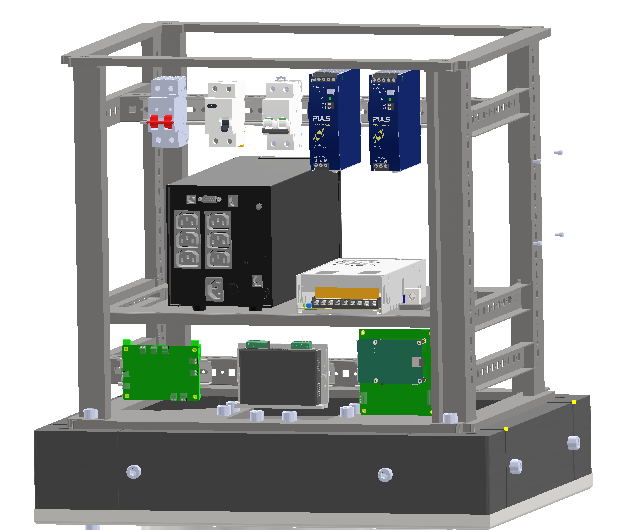
\includegraphics[width=0.92\linewidth,height=0.62\textheight,keepaspectratio]{./media/image73.png}
\captionof*{figure}{\small\itshape Figura 80. Rack con componentes}
\addcontentsline{lof}{figure}{Figura 80. Rack con componentes}
\label{fig:80}
\end{center}

\subsection{Análisis térmico}\label{anuxe1lisis-tuxe9rmico}

El análisis térmico verifica que la temperatura interna del gabinete permanezca dentro de límites operativos de los componentes electrónicos bajo condiciones ambientales extremas. Los componentes más sensibles (Raspberry Pi, HAT 4G LTE) especifican temperatura operativa máxima de 70-85°C, mientras que componentes de potencia (SMPS, UPS, driver) toleran hasta 105°C en puntos calientes internos.

\textbf{Cálculo de generación de calor:}

La potencia eléctrica disipada como calor en el interior del gabinete proviene de pérdidas en conversión de energía y consumo de componentes electrónicos. Se estiman las siguientes contribuciones:

\textbf{SMPS S-360-24 (eficiencia 85\%):}

Potencia de salida máxima:

\begin{centeredmath}
\ \ \ \ \ \ \ \ \ P_{out} = 24V\  \times \ 15A\  = \ 360W\quad \ \ \ \ \ \ \ \ \ \ \ \ \ \ \ \ \ \ \ \ \ \ \ \ \ \ \ \ \ \ \ \ \ \ \ \ \ \ \ \ \ \ \ \ \ \ \ \ \ \ \ \ \ \ \ \ \ \ \ \ \ (1)\
\end{centeredmath}

Pérdidas:

\begin{centeredmath}
\ \ \ \ \ \ \ \ \ \ \ \ \ \ \ \ \ \ \ \ P_{\text{pérdidas SMPS}} = P_{out}\ x\ (1 - n)/n\  = 360\ x\ (1 - 0.85)/0.85\quad \ \ \ \ \ \ \ \ \ \ \ \ \ \ \ \ \ \ \ \ \ \ \ \ \ (2)\
\end{centeredmath}

\begin{centeredmath}
\ \ \ \ \ \ \ \ \ \ \ \ \ \ \ \ \ \ \ \ \ \ \ \ \ \ \ \ \ \ \ \ \ \ \ \ \ \ \ \ \ \ \ \ \ \ \ \ \ \ \ \ \ \ \ P_{\text{pérdidas SMPS}} = 63.5\ W\quad \ \ \ \ \ \ \ \ \ \ \ \ \ \ \ \ \ \ \ \ \ \ \ \ \ \ \ \ \ \ \ \ \ \ \ \ \ \ \ \ \ \ \ \ \ \ \ \ \ \ \ \ \ \ \ \ \ \ \ \ \ \ (3)\
\end{centeredmath}

\textbf{UPS 500VA (operación float charging, eficiencia 92\%):}

\begin{centeredmath}
\ \ \ \ \ \ \ \ \ \ \ \ \ \ \ \ \ \ \ \ P_{\text{pérdidas UPS}} = 500\ x\ 0.08\  = \ 40\ W\ (En\ modo\ recarga)\quad \ \ \ \ \ \ \ \ \ \ \ \ \ \ \ \ \ \ \ \ \ \ \ \ \ \ \ \ \ \ \ \ \ (4)\
\end{centeredmath}

\textbf{Driver DM542T (operación motor a 3A, eficiencia 90\%):}

Potencia entregada al motor:

\begin{centeredmath}
\ \ \ \ \ \ \ \ \ \ \ \ \ \ \ \ \ \ \ \ \ \ \ \ \ \ \ \ \ \ \ \ \ \ P_{motor} = 24V\  \times \ 3A\  \times \ 2\ fases\  = \ 144W\quad \ \ \ \ \ \ \ \ \ \ \ \ \ \ \ \ \ \ \ \ \ \ \ \ \ \ \ \ \ \ \ \ \ \ \ \ \ \ \ \ \ \ \ \ \ \ \ \ \ \ \ (5)\
\end{centeredmath}

\begin{centeredmath}
\ \ \ \ \ \ \ P_{\text{pérdidas driver}} = \ 144\  \times \ (1\  - \ 0.90)\ /\ 0.90\  = \ 16W\quad \ \ \ \ \ \ \ \ \ \ \ \ \ \ \ \ \ \ \ \ \ \ \ \ \ \ \ \ \ \ \ \ \ \ \ \ \ \ \ \ \ \ \ (6)\
\end{centeredmath}

\textbf{Raspberry Pi 5 (consumo bajo carga):}

\begin{centeredmath}
\ \ \ \ \ \ \ \ \ \ \ \ P_{Raspberry} = \ 15W\quad \ \ \ \ \ \ \ \ \ \ \ \ \ \ \ \ \ \ \ \ \ \ \ \ \ \ \ \ \ \ \ \ \ \ \ \ \ \ \ \ \ \ \ \ \ \ \ \ \ \ \ \ \ \ \ \ \ \ \ \ \ \ \ \ \ \ \ \ \ \ \ (7)\
\end{centeredmath}

\textbf{HAT 4G LTE (transmisión activa):}

\begin{centeredmath}
\ \ \ \ \ \ \ \ \ \ \ \ {\ \ \ \ \ P}_{HAT} = \ 5W\quad \ \ \ \ \ \ \ \ \ \ \ \ \ \ \ \ \ \ \ \ \ \ \ \ \ \ \ \ \ \ \ \ \ \ \ \ \ \ \ \ \ \ \ \ \ \ \ \ \ \ \ \ \ \ \ \ \ \ \ \ \ \ \ \ \ \ \ \ \ \ \ \ \ \ \ \ \ \ (8)\
\end{centeredmath}

\textbf{Conversores DC-DC (eficiencia 85\%):}

\begin{centeredmath}
\ \ \ \ \ \ \ \ \ \ \ \ \ \ \ \ \ \ \ \ P_{\text{pérdidas conversores}} = \ (5V\  \times \ 3A\  + \ 12V\  \times \ 2A)\  \times \ 0.15\ /\ 0.85\  = \ 8.4W\quad \ \ \ \ \ \ \ \ \ \ \ \ \ \ \ \ \ \ \ \ (9)\
\end{centeredmath}

\textbf{Potencia térmica total disipada (usando (1) al (9)):}

\begin{centeredmath}
\ \ \ \ \ \ \ \ \ \ \ \ \ \ \ \ \ \ \ \ Q_{TOTAL}\  = \ 63.5\  + \ 40\  + \ 16\  + \ 15\  + \ 5\  + \ 8.4\  = \ 147.9\ W\  \approx \ 150W\quad \ \ \ \ \ \ \ \ \ \ \ \
\end{centeredmath}

\textbf{Sistema de ventilación:}

Para evacuar los 150W de calor generado y mantener temperatura interna aceptable, se implementa ventilación forzada mediante ventilador axial de 120 \ensuremath{\times} 120 mm ubicado en la parte superior del gabinete, expulsando aire caliente hacia el exterior. El aire fresco ingresa por rejillas inferiores frontales con filtro de polvo lavable.

Especificaciones del ventilador:

• Dimensiones: 120 \ensuremath{\times} 120 \ensuremath{\times} 38 mm

• Voltaje de operación: 24V DC

• Consumo de potencia: 12W

• Caudal nominal: 180 m\ensuremath{^{3}}/h = 0.05 m\ensuremath{^{3}}/s

• Presión estática: 80 Pa

El incremento de temperatura del aire al atravesar el gabinete se calcula mediante balance térmico:

Q = \ensuremath{\dot{m}} \ensuremath{\times} c\_p \ensuremath{\times} \ensuremath{\Delta}T (1)

Donde:

Q = 150W = potencia térmica a evacuar

\ensuremath{\dot{m}} = \(\rho_{aire}\) \ensuremath{\times} V = masa de aire circulante por unidad de tiempo

\(\rho_{aire}\)= 1.2 kg/m\ensuremath{^{3}} (densidad del aire a 20°C)

V = 0.05 m\ensuremath{^{3}}/s (caudal del ventilador)

\(c_{p}\) = 1005 J/(kg·K) (calor específico del aire)

Flujo másico de aire:

\ensuremath{\dot{m}} = 1.2 kg/m\ensuremath{^{3}} \ensuremath{\times} 0.05 m\ensuremath{^{3}}/s = 0.06 kg/s (2)

Elevación de temperatura usando (1) y (2):

\ensuremath{\Delta}T = Q / (\ensuremath{\dot{m}} \ensuremath{\times} c\_p) = 150W / (0.06 kg/s \ensuremath{\times} 1005 J/(kg·K))

\ensuremath{\Delta}T = 150 / 60.3 = 2.5°C

Este resultado indica que el aire se calienta 2.5°C al pasar por el gabinete cuando el ventilador opera a capacidad nominal. En el caso más desfavorable de temperatura ambiente de 60°C (límite superior especificado), la temperatura del aire expulsado sería aproximadamente 62.5°C, manteniendo la temperatura interna promedio alrededor de 61°C, dentro del rango operativo de todos los componentes. (Ventilador y salida en la Figura 77)

\begin{center}
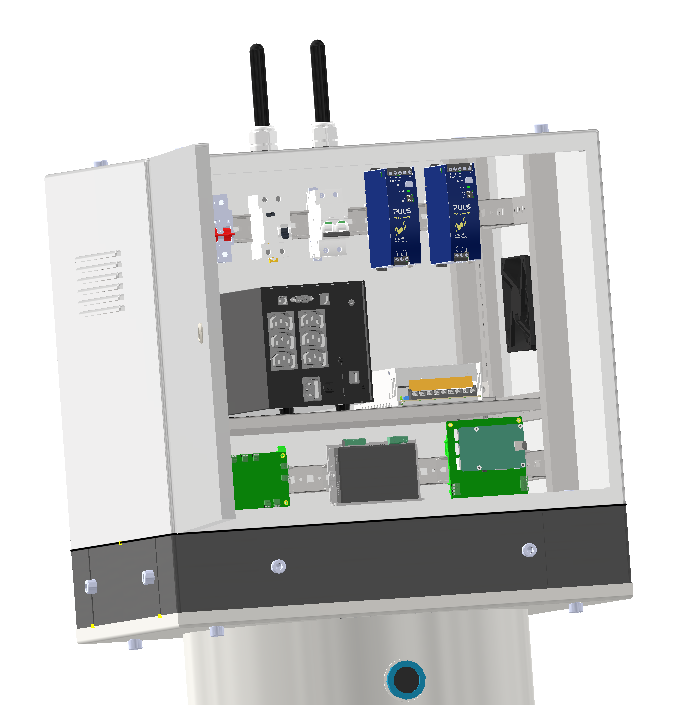
\includegraphics[width=0.92\linewidth,height=0.62\textheight,keepaspectratio]{./media/image29.png}
\captionof*{figure}{\small\itshape Figura 81. Vista del Ventilador y Salida de aire}
\addcontentsline{lof}{figure}{Figura 81. Vista del Ventilador y Salida de aire}
\label{fig:81}
\end{center}

\section{Diseño del soporte del controlador semafórico}\label{diseuxf1o-del-soporte-del-controlador-semafuxf3rico}

Presentación del diseño mecánico del soporte destinado al controlador semafórico, su geometría, puntos de anclaje y condiciones de operación.

\begin{center}
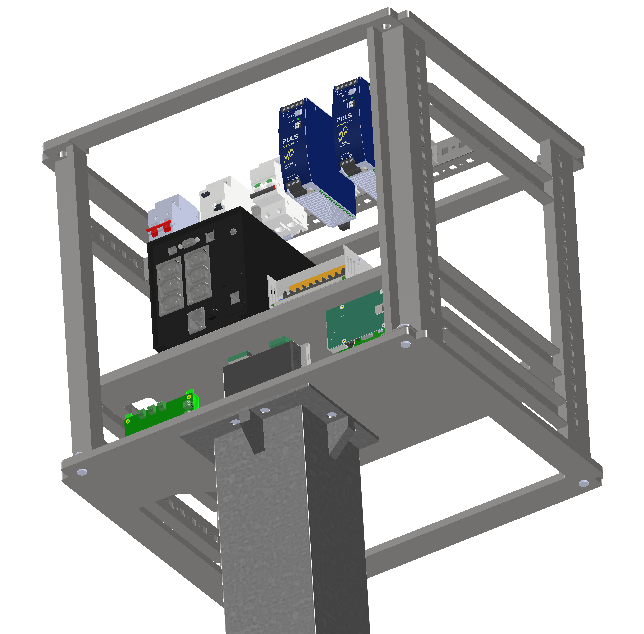
\includegraphics[width=0.92\linewidth,height=0.62\textheight,keepaspectratio]{./media/image104.png}
\captionof*{figure}{\small\itshape Figura 82. Vista de conexión Rack y Poste de Acero cuadrático}
\addcontentsline{lof}{figure}{Figura 82. Vista de conexión Rack y Poste de Acero cuadrático}
\label{fig:82}
\end{center}

\subsection{Cálculos estructurales}\label{cuxe1lculos-estructurales-1}

El sistema soporta un gabinete con masa total de 47.126 kg posicionado a 4.8 m de altura sobre el nivel del terreno. El peso total genera una carga vertical de:

\begin{centeredmath}
\ \ \ \ \ \ \ \ \ Wgabinete\  = \ 47.126\ kg\  \times \ 9.81\ m/s\ensuremath{^{2}}\  = 462\ N\quad \ \ \ \ \ \ \ \ \ \ \ \ \ \ \ \ \ \ \ \ \ \ \ \ \ \ \ \ \ \ \ \ \ (1)\
\end{centeredmath}

Sin embargo, para el análisis estructural se adoptará una carga simplificada conservadora de 35 kg (343 N) según lo establecido en los criterios de diseño, lo cual proporciona un margen adicional de seguridad considerando que parte de la masa corresponde a componentes removibles durante el mantenimiento.

\begin{centeredmath}
\ \ \ \ \ \ \ \ \ \ \ \ \ \ \ \ \ \ \ \ \ \ W_{\text{diseño}}\  = \ 35\ kg\  \times \ 9.81\ m/s\ensuremath{^{2}}\  = \ 343.4\ N\  \approx \ 350\ N\quad \ \ \ \ \ \ \ \ \ \ \ \ \ \ \ \ \ \ \ \ \ \ \ \ \ \ \ \ \ \ \ (2)\
\end{centeredmath}

El poste se fabrica mediante perfil tubular cuadrado hueco de acero estructural A36 con las siguientes características geométricas:

\textbf{Dimensiones:}

\begin{itemize}
\item
  Altura total: H = 4800 mm
\item
  Sección transversal: 130 \ensuremath{\times} 130 mm (cuadrada)
\item
  Espesor de pared: t = 10 mm
\item
  Área de sección transversal neta:
\end{itemize}

\begin{centeredmath}
\ \ \ \ \ \ \ \ \ \ \ \ \ \ A\  = \ (130\ensuremath{^{2}})\  - \ (110\ensuremath{^{2}})\  = \ 16,900\  - \ 12,100\  = \ 4,800\ mm\ensuremath{^{2}}\quad \ \ \ \ \ \ \ \ \ \ \ \ \ \ \ \ \ \ \ \ \ \ \ \ (3)\
\end{centeredmath}

\textbf{Propiedades geométricas de la sección:}

Momento de inercia de sección cuadrada hueca respecto a ejes principales:

\begin{centeredmath}
\ \ \ \ \ \ \ \ \ \ \ \ \ \ I\  = \ (b\ensuremath{_{4}}\ensuremath{^{4}}\  - \ b\ensuremath{_{1}}\ensuremath{^{4}})/12\  = \ (130\ensuremath{^{4}}\  - \ 110\ensuremath{^{4}})/12\quad \ \ \ \ \ \ \ \ \ \ \ \ \ \ \ \ \ \ \ \ \ \ \ \ \ \ \ \ \ \ \ \ \ \ \ \ (4)\
\end{centeredmath}

\begin{centeredmath}
\ \ \ \ \ \ \ \ \ \ \ \ \ I\  = \ 11,600,000\ mm\ensuremath{^{4}}\ \quad \ \ \ \ \ \ \ \ \ \ \ \ \ \ \ \ \ \ \ \ \ \ \ \ \ \ \ \ \ \ \ \ \ \ \ \ \ \ \ \ \ \ \ \ \ \ \ \ \ \ \ \ \ \ \ \ \ \ \ \ \ \ \ (5)\
\end{centeredmath}

Módulo de sección elástico:

\begin{centeredmath}
\ \ \ \ \ \ \ \ \ \ \ \ \ W\  = \ I/(b/2)\  = \ 11,600,000/(130/2)\  = \ 178,462\ mm\ensuremath{^{3}}\ \quad \ \ \ \ \ \ \ \ \ \ \ \ \ \ \ \ \ \ \ (6)\
\end{centeredmath}

Radio de giro:

\begin{centeredmath}
\ \ \ \ \ \ \ \ \ \ \ \ \ r\  = \ \sqrt{}(I/A)\  = \ \sqrt{}(11,600,000/4,800)\  = \ \sqrt{}2,417\  = \ 49.2\ mm\ \quad \ \ \ \ \ \ \ \ \ \ \ (7)\
\end{centeredmath}

\textbf{Propiedades del material - Acero A36:}

Resistencia a la fluencia: fy = 250 MPa

Resistencia última a tracción: fu = 400 MPa

Módulo de elasticidad: E = 200,000 MPa

Densidad: \ensuremath{\rho} = 7,850 kg/m\ensuremath{^{3}}

La carga axial de compresión en el poste debido al peso del gabinete genera un esfuerzo normal de

\ensuremath{\sigma}compresión =

\begin{centeredmath}
\ \ \ \ \ \ \ \ \ \ W_{\text{diseño}}\ /\ A\  = \ 350\ N\ /\ 4,800\ mm\ensuremath{^{2}}\  = \ 0.073\ N/mm\ensuremath{^{2}}\  = \ 0.073\ MPa\ \quad \ \ \ \ \ \ (8)\
\end{centeredmath}

Factor de seguridad respecto a fluencia del material:

\begin{centeredmath}
\ \ \ \ \ \ \ \ \ \ \ \ \ \ \ \ \ \ \ FS_{\text{compresión}}\  = \ f_{y}\ /\ \sigma_{\text{compresión}}\  = \ 250\ MPa\ /\ 0.073\ MPa\  = \ 3,425\ \quad \ \ \ \ \ \ (9)\
\end{centeredmath}

Este factor de seguridad extremadamente alto (\textgreater3400) confirma que la carga gravitatoria pura es insignificante para el dimensionamiento del poste. El diseño estructural está dominado por cargas laterales de viento que generan momentos flectores, no por cargas axiales de compresión.

\textbf{Justificación del posicionamiento del gabinete respecto al centro de masa}

El gabinete se posiciona estratégicamente en el poste de modo que su centro de masa (calculado en sección 5.1.3 en coordenadas X=273.2 mm, Y=223.9 mm, Z=254.9 mm desde la esquina inferior posterior izquierda) se ubique lo más próximo posible al eje vertical del poste.

Según el análisis de centro de masa, la posición óptima del punto de apoyo del poste es a 110 mm desde el frente del gabinete. Esta ubicación minimiza la excentricidad entre el centro de masa del gabinete (273.2 mm desde el borde posterior) y el eje del poste, resultando en una excentricidad de:

\begin{centeredmath}
\ \ \ \ \ \ \ \ \ \ \ \ \ e\  = \ 273.2\ mm\  - \ 110\ mm\  = \ 163.2\ mm\  \approx \ 160\ mm\ \quad \ \ \ \ \ \ \ \ \ \ \ \ \ \ \ \ \ \ \ \ \ \ \ \ (10)\
\end{centeredmath}

Esta excentricidad reducida amortigua el momento flector adicional generado por el peso del gabinete:

\begin{centeredmath}
\ \ \ \ \ \ \ \ \ \ \ \ \ M_{\text{excentricidad}}\  = \ W_{\text{diseño}}\  \times \ e\  = \ 350\ N\  \times \ 0.160\ m\  = \ 56\ N \cdot m\ \quad \ \ \ \ \ \ \ \ \ \ \ (11)\
\end{centeredmath}

Si el gabinete estuviera centrado geométricamente (sin considerar centro de masa), la excentricidad sería mayor, incrementando el momento en aproximadamente 10\%. El posicionamiento optimizado reduce los esfuerzos en el poste y en las soldaduras de conexión gabinete-poste, además de facilitar el ruteo de cables de alimentación y comunicaciones desde el interior del poste hacia el gabinete sin crear interferencias mecánicas con componentes internos.

\textbf{Refuerzos triangulares superiores}

\begin{center}
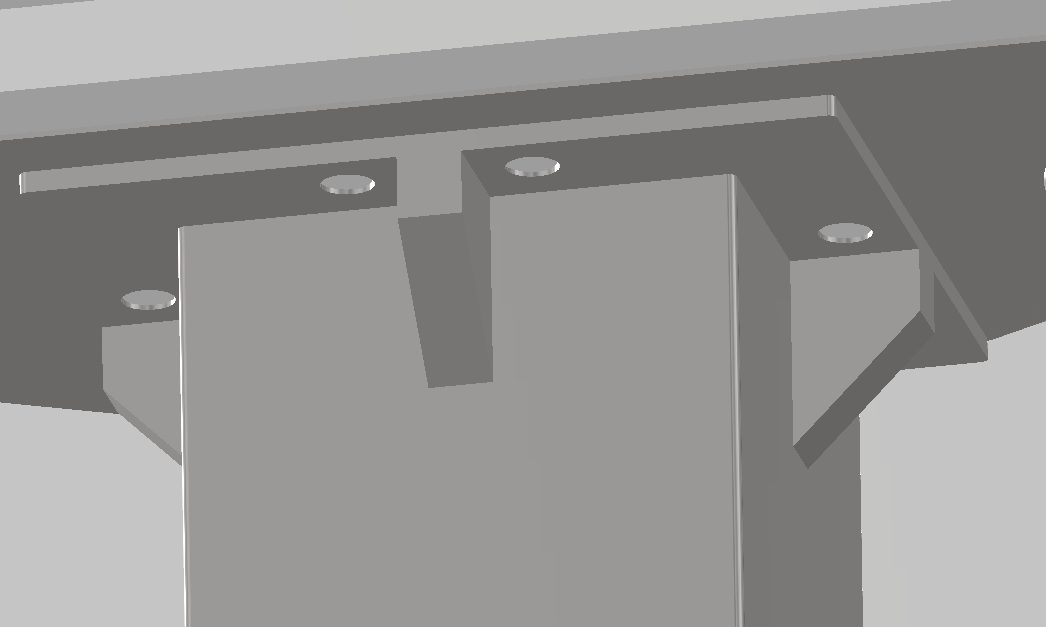
\includegraphics[width=0.92\linewidth,height=0.62\textheight,keepaspectratio]{./media/image55.png}
\captionof*{figure}{\small\itshape Figura 83. Refuerzos triangulares superiores}
\addcontentsline{lof}{figure}{Figura 83. Refuerzos triangulares superiores}
\label{fig:83}
\end{center}

Cantidad: 3 refuerzos (uno por cada cara lateral del poste, excepto cara posterior)

Longitud: L = 50 mm

Ángulo: \ensuremath{\alpha} = 45°

Ubicación: En la parte superior del poste, en zona de conexión gabinete-poste

Material: Placa de acero A36 de espesor 6 mm

Los refuerzos triangulares superiores cumplen dos funciones críticas:

1. Rigidización de la zona de conexión gabinete-poste:

La unión entre el gabinete de aluminio (base abierta) y el poste de acero genera una discontinuidad estructural donde se concentran tensiones. Los refuerzos triangulares distribuyen estas tensiones en un área mayor, evitando concentraciones que podrían iniciar grietas por fatiga.

2. Resistencia al momento flector:

El momento generado por cargas laterales de viento sobre el gabinete crea esfuerzos cortantes en la interfaz gabinete-poste. Los refuerzos actúan como ménsulas que transfieren estos esfuerzos cortantes desde el gabinete hacia el poste de manera gradual, reduciendo picos de esfuerzo.

\textbf{Refuerzos triangulares inferiores}

\begin{center}
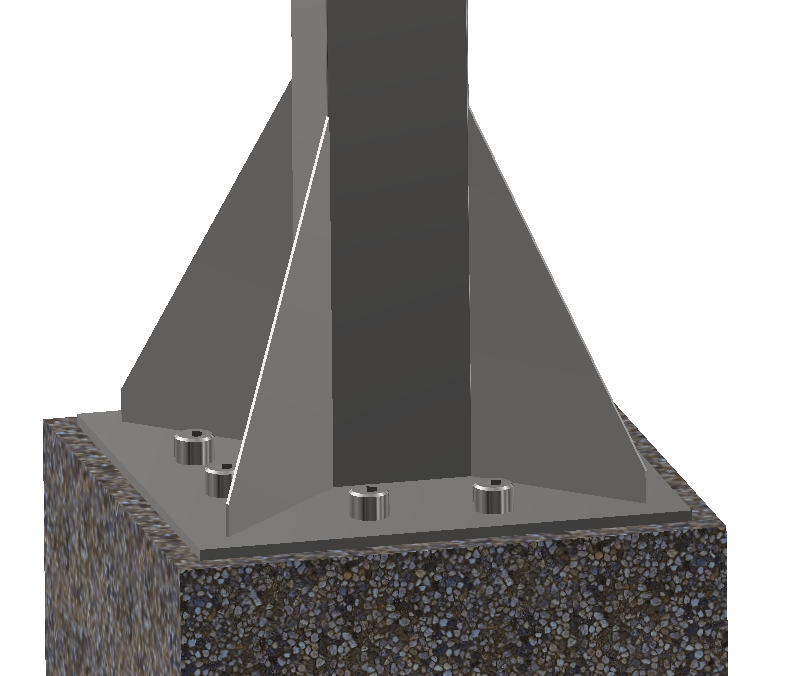
\includegraphics[width=0.92\linewidth,height=0.62\textheight,keepaspectratio]{./media/image159.png}
\captionof*{figure}{\small\itshape Figura 84. Refuerzos triangulares inferiores}
\addcontentsline{lof}{figure}{Figura 84. Refuerzos triangulares inferiores}
\label{fig:84}
\end{center}

Cantidad: 4 refuerzos (uno por cada cara del poste)

Longitud: L = 350 mm

Ángulo: \ensuremath{\alpha} = 23°

Base: b = 130 mm (coincidente con el ancho del poste)

Ubicación: En la base del poste, zona de transición poste-zapata

Material: Placa de acero A36 de espesor 8 mm

Los refuerzos triangulares inferiores cumplen funciones estructurales críticas que justifican sus dimensiones significativamente mayores que los superiores:

1. Transferencia del momento de vuelco a la cimentación:

El momento flector máximo en la estructura se presenta en la base del poste, donde se acumula el efecto de todas las cargas laterales multiplicadas por la altura de 4.8 m. Los refuerzos inferiores funcionan como vigas en voladizo invertidas que distribuyen este momento sobre un área mayor de la zapata, reduciendo las presiones de contacto concreto-acero.

2. Prevención de pandeo local en la base:

La transición entre el poste (elemento flexible y esbelto) y la zapata (elemento rígido y masivo) genera una zona de alta concentración de esfuerzos cortantes. Sin refuerzos, las paredes del perfil tubular podrían experimentar pandeo local por compresión. Los refuerzos a 23° proporcionan rigidez adicional que previene este modo de falla.

3. Anclaje estructural:

Los refuerzos se sueldan tanto al poste como a una placa base embebida en la zapata, creando una conexión de momento completo (empotramiento) que garantiza que el poste trabaje como viga en voladizo desde la base, no como columna articulada. Esto maximiza la rigidez del sistema y minimiza deflexiones en la punta.

\textbf{Diseño de la zapata de cimentación}

\begin{center}
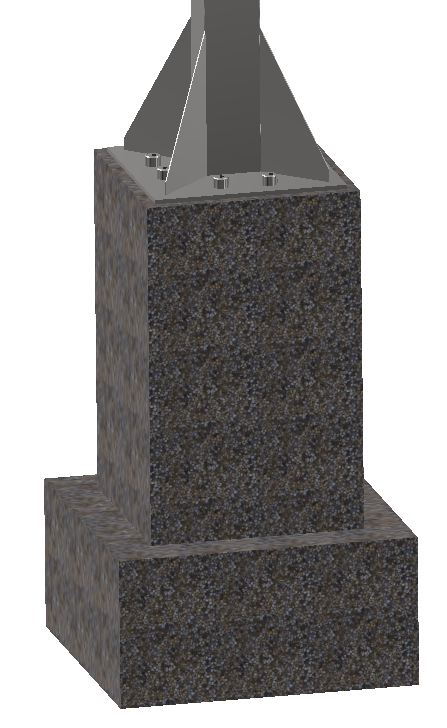
\includegraphics[width=0.92\linewidth,height=0.62\textheight,keepaspectratio]{./media/image90.png}
\captionof*{figure}{\small\itshape Figura 85. Zapata de cimentación}
\addcontentsline{lof}{figure}{Figura 85. Zapata de cimentación}
\label{fig:85}
\end{center}

La zapata de hormigón armado cumple dos funciones estructurales primarias, una es distribuir las cargas concentradas del poste sobre un área suficiente de suelo para no exceder su capacidad portante, y proporcionar masa y geometría adecuadas para resistir el momento de vuelco generado por cargas laterales de viento sin levantar del suelo.

La zapata presenta geometría escalonada en dos niveles:

Nivel superior (pedestal):

Sección transversal: 500 \ensuremath{\times} 500 mm

Altura: 800 mm

Nivel inferior (zapata propiamente dicha):

Sección transversal: 700 \ensuremath{\times} 700 mm

Altura: 350 mm

El pedestal sobresale parcialmente del terreno para elevar el punto de conexión con el poste y evitar acumulación de agua en la base. El nivel inferior es más ancho para distribuir las cargas sobre mayor área del suelo.

\begin{center}
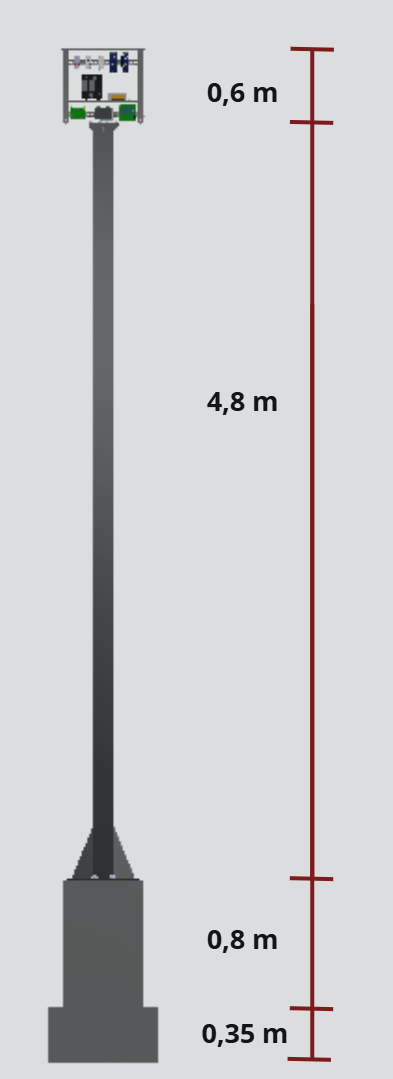
\includegraphics[width=0.92\linewidth,height=0.62\textheight,keepaspectratio]{./media/image96.png}
\captionof*{figure}{\small\itshape Figura 86. Vista de conexión Rack y Poste de Acero cuadrático}
\addcontentsline{lof}{figure}{Figura 86. Vista de conexión Rack y Poste de Acero cuadrático}
\label{fig:86}
\end{center}

\subsection{Selección de materiales}\label{selecciuxf3n-de-materiales}

Cada material ha sido seleccionado específicamente para la función estructural que desempeña en el sistema.

\textbf{Poste: Acero estructural A36}

El poste se fabrica mediante perfil tubular cuadrado hueco de acero estructural ASTM A36, material utilizado en estructuras urbanas expuestas a intemperie por su combinación óptima de propiedades mecánicas, disponibilidad comercial y costo.

\textbf{Propiedades mecánicas:}

\begin{itemize}
\item
  Resistencia a la fluencia: fy = 250 MPa
\item
  Resistencia última a tracción: fu = 400 MPa
\item
  Módulo de elasticidad: E = 200,000 MPa
\item
  Densidad: \ensuremath{\rho} = 7,850 kg/m\ensuremath{^{3}}
\end{itemize}

\textbf{Justificación de selección:}

El acero A36 proporciona resistencia mecánica superior (250 MPa vs 193 MPa del aluminio 5052-H32) necesaria para resistir momentos flectores elevados generados por cargas de viento a 4.8 m de altura. Su módulo de elasticidad de 200 GPa, casi tres veces mayor que el aluminio (70 GPa), minimiza deflexiones laterales del poste, críticas para mantener verticalidad del gabinete y evitar desalineamientos.

\textbf{Protección contra corrosión:}

El ambiente marino salino de Lima requiere protección anticorrosiva robusta. El poste se protege mediante sistema de recubrimiento multicapa:

\begin{enumerate}
\def\labelenumi{\arabic{enumi}.}
\item
  \textbf{Galvanización por inmersión en caliente:} Aplicación de zinc según norma NTP-ISO, proporcionando protección catódica que previene corrosión del acero base incluso si el recubrimiento se daña superficialmente.
\item
  \textbf{Pintura de acabado:} Aplicación de pintura de poliuretano con resistencia UV sobre galvanizado, proporcionando doble barrera protectora y acabado estético. Espesor total del sistema de pintura: 120-150 \ensuremath{\mu}m en dos capas (imprimación + acabado).
\end{enumerate}

De esta forma el sistema cumple la normativa municipal MML para protección de estructuras metálicas expuestas.

\textbf{Gabinete: Aleación de aluminio 5052-H32}

El gabinete se fabrica en aleación de aluminio 5052-H32 con espesor de 6 mm, como se detalló extensamente en la sección 5.1.4. La selección de este material se fundamenta en ventajas estructurales como bajo peso por su densidad menor al del aluminio, resistencia a corrosión por contenido de magnesio, conductividad térmica alta favoreciendo disipación de calor generado por los componentes internos.

\textbf{Compatibilidad estructural gabinete-poste:}

La interfaz entre gabinete de aluminio y poste de acero requiere consideraciones especiales por la diferencia en propiedades de materiales. Amerita aislamiento galvánico por diferencia de potencial electroquímico entre ambos materiales.

\textbf{Zapata: Hormigón armado}

La zapata de cimentación se construye mediante hormigón armado de resistencia característica f\textquotesingle c = 210 kg/cm\ensuremath{^{2}} (21 MPa), valor estándar en construcciones urbanas de Lima que proporciona capacidad estructural adecuada con economía de materiales.

\section{Simulación y verificación de resistencia}\label{simulaciuxf3n-y-verificaciuxf3n-de-resistencia}

Para validar el diseño estructural del sistema completo (gabinete, rack interno, poste de soporte y zapata de cimentación) bajo condiciones de servicio extremas, se realizó análisis por elementos finitos (FEA) mediante software Autodesk Inventor Professional. El análisis considera cargas gravitatorias, cargas laterales de viento, y condiciones de frontera que representan el comportamiento estructural del sistema instalado en intersección vehicular.

\subsection{Condiciones de simulación y cargas aplicadas}\label{condiciones-de-simulaciuxf3n-y-cargas-aplicadas}

\textbf{Modelo geométrico}

El modelo de elementos finitos incluye todos los componentes estructurales del sistema:

\begin{itemize}
\item
  \textbf{Gabinete de aluminio 5052-H32:} Geometría de cubo hueco sin base inferior con espesor de 6 mm, incluyendo refuerzos de conexión al poste
\item
  \textbf{Rack interno:} Perfiles de aluminio 30\ensuremath{\times}30 mm y bandejas perforadas con componentes electrónicos modelados como masas concentradas en sus posiciones reales
\item
  \textbf{Poste de acero A36:} Perfil tubular cuadrado 130\ensuremath{\times}130\ensuremath{\times}10 mm con altura de 4,800 mm
\item
  \textbf{Refuerzos triangulares:} Superiores (50 mm, 45°, espesor 6 mm) e inferiores (350 mm, 23°, espesor 8 mm)
\item
  \textbf{Placa base:} Placa de acero 400\ensuremath{\times}400\ensuremath{\times}20 mm en la base del poste
\item
  \textbf{Sistema de movimiento:} Aro estructural, rodamiento, biela y conector de cámara
\end{itemize}

\textbf{Cargas aplicadas}

El análisis considera un escenario conservador de carga extrema que excede las condiciones nominales de operación para verificar reservas de resistencia del diseño:

\textbf{1. Cargas gravitatorias:}

\begin{itemize}
\item
  Peso propio de todos los componentes estructurales (calculado automáticamente por el software en función de densidades y geometrías)
\item
  Masa del rack con componentes electrónicos: 11.965 kg distribuida según posiciones reales
\item
  Masa del sistema de movimiento: 11.299 kg en zona inferior del gabinete
\item
  Aceleración gravitatoria: g = 9.81 m/s\ensuremath{^{2}} en dirección vertical (-Y)
\end{itemize}

\textbf{2. Cargas de viento:}

Se aplicó presión lateral uniforme sobre las superficies expuestas del gabinete simulando carga de viento extrema. La presión de diseño adoptada es q = 1,500 Pa (1.5 kPa), valor que corresponde a velocidad de viento de aproximadamente 175 km/h

Esta presión de 1.5 kPa excede significativamente la presión de viento de diseño normativa de 1.0 kPa (velocidad \textasciitilde145 km/h, tiempo de retorno 50 años según AASHTO), proporcionando margen de seguridad adicional y simulando condiciones extremas poco probables durante la vida útil del sistema. La presión se aplicó perpendicularmente a las superficies frontales (600 \ensuremath{\times} 525 mm) y laterales (479 \ensuremath{\times} 525 mm) del gabinete.

Las superficies inferiores de la placa base (400\ensuremath{\times}400 mm) se restringieron completamente en todos los grados de libertad, simulando la conexión rígida con la zapata de hormigón mediante barras de anclaje.

\subsection{Análisis de tensiones de Von Mises}\label{anuxe1lisis-de-tensiones-de-von-mises}

La tensión de Von Mises (tensión equivalente) es el criterio de falla más utilizado para materiales dúctiles como aluminio y acero, ya que predice el inicio de fluencia plástica considerando el estado triaxial de los esfuerzos. La teoría establece que la fluencia ocurre cuando la tensión de Von Mises alcanza el límite elástico del material.

\textbf{Distribución de tensiones en el sistema completo}

El análisis reveló que la tensión máxima de Von Mises se localiza en la cubierta del sistema de vigilancia junto con el poste con una tensión de valor 46.28 MPa. Esta concentración de esfuerzo se debe a la discontinuidad geométrica en la zona de transición entre el aro estructural de aluminio (cubierta del sistema de vigilancia con masa de 7.8 kg) y el perfil tubular del poste, donde se genera transferencia de cargas combinadas: el peso del sistema de visión completo (11.3 kg incluyendo motor, rodamiento, biela y cámara) más el momento flector inducido por la presión lateral de viento sobre el área expuesta del aro circular (Ø420 mm). La geometría circular del aro concentra tensiones en los puntos de unión con el poste debido al cambio brusco de sección transversal (de perfil cuadrado 130\ensuremath{\times}130 mm a geometría circular) y al hecho de que esta zona actúa como ménsula en voladizo soportando tanto cargas gravitatorias como laterales. Observado en la Figura 87 y 88.

\begin{center}
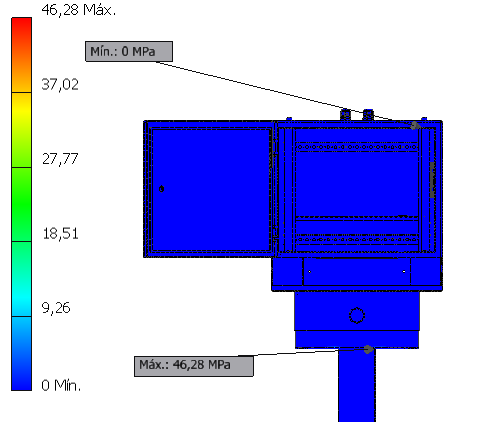
\includegraphics[width=0.92\linewidth,height=0.62\textheight,keepaspectratio]{./media/image134.png}
\captionof*{figure}{\small\itshape Figura 87. Distribución de tensión de Von Mises en sistema completo}
\addcontentsline{lof}{figure}{Figura 87. Distribución de tensión de Von Mises en sistema completo}
\label{fig:87}
\end{center}

\begin{center}
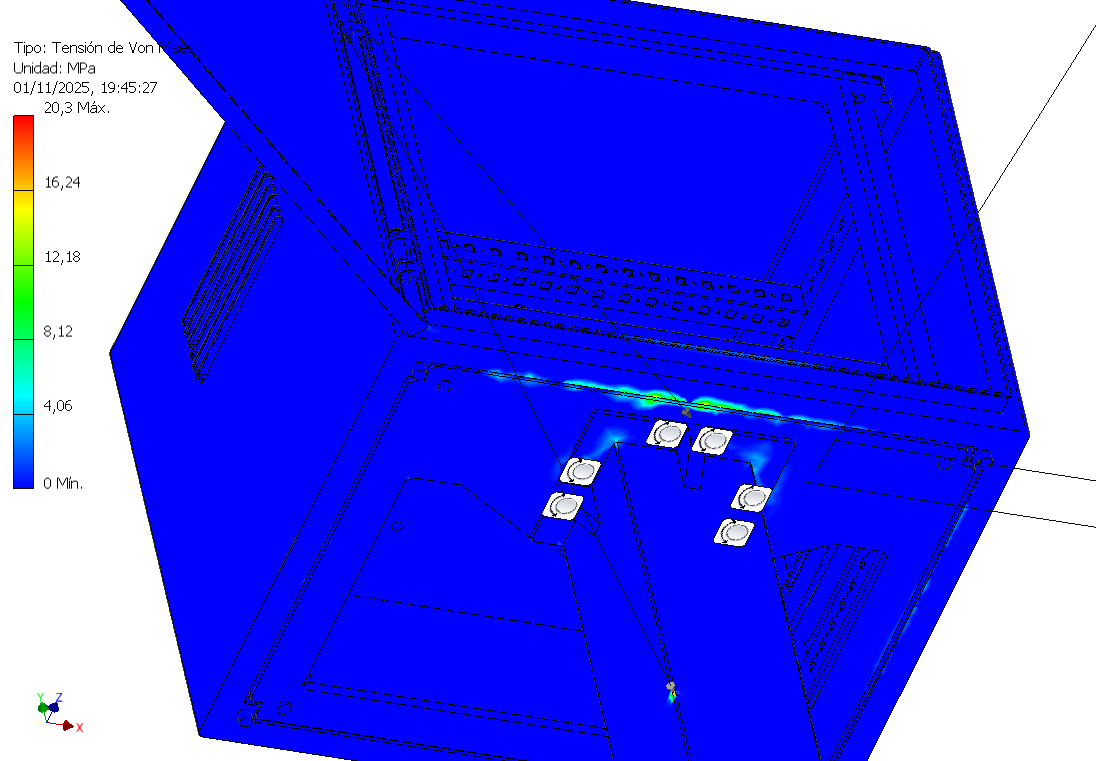
\includegraphics[width=0.92\linewidth,height=0.62\textheight,keepaspectratio]{./media/image31.png}
\captionof*{figure}{\small\itshape Figura 88. Distribución de tensión de Von Mises Vista Inferior del Gabinete}
\addcontentsline{lof}{figure}{Figura 88. Distribución de tensión de Von Mises Vista Inferior del Gabinete}
\label{fig:88}
\end{center}

La distribución de tensiones muestra que:

\begin{itemize}
\item
  \textbf{Gabinete:} Las tensiones permanecen predominantemente bajas en la mayor parte de la estructura, con elevaciones locales en las esquinas de conexión con el poste donde se transfieren cargas de viento.
\item
  \textbf{Rack interno:} Los perfiles verticales del rack experimentan tensiones de en las zonas de fijación de componentes pesados (UPS 3.5 kg, SMPS 1.2 kg).
\item
  \textbf{Poste de acero:} Las tensiones son mínimas en la mayor parte de la longitud del poste, confirmando que el dimensionamiento está controlado por rigidez (deflexiones) más que por resistencia.
\end{itemize}

La tensión máxima del sistema (46.28 MPa) está significativamente por debajo de los límites elásticos del aluminio 5052-H32 (193 MPa) y acero A36 (250 MPa), confirmando operación en rango elástico con margen de seguridad adecuado.

\subsection{Análisis de tensiones principales}\label{anuxe1lisis-de-tensiones-principales}

Las tensiones principales (\ensuremath{\sigma}\ensuremath{_{1}}, \ensuremath{\sigma}\ensuremath{_{2}}, \ensuremath{\sigma}\ensuremath{_{3}}) representan los esfuerzos normales máximo, intermedio y mínimo en cada punto del material, actuando sobre planos perpendiculares entre sí donde los esfuerzos cortantes son nulos. El análisis de tensiones principales proporciona información adicional sobre el estado de esfuerzo que complementa el criterio de Von Mises.

\textbf{Primera tensión principal (\ensuremath{\sigma}\ensuremath{_{1}}) - Tensión de tracción máxima}

La primera tensión principal representa el mayor esfuerzo de tracción en cada punto. Valores positivos indican tracción pura, críticos para materiales frágiles o para evaluar riesgo de fatiga.

\begin{center}
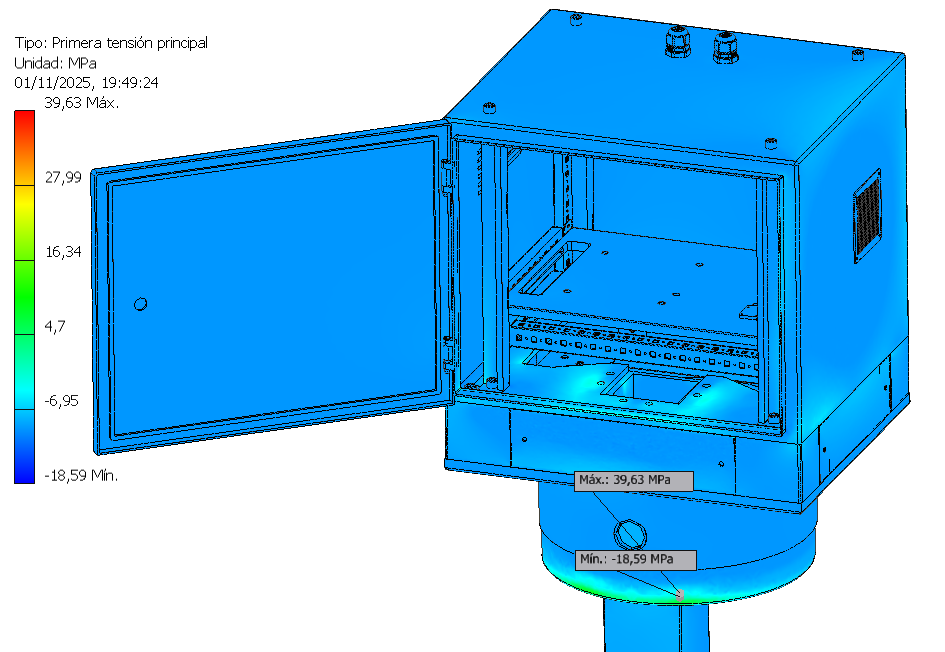
\includegraphics[width=0.92\linewidth,height=0.62\textheight,keepaspectratio]{./media/image100.png}
\captionof*{figure}{\small\itshape Figura 89. Distribución de primera tensión principal}
\addcontentsline{lof}{figure}{Figura 89. Distribución de primera tensión principal}
\label{fig:89}
\end{center}

El análisis muestra:

\begin{itemize}
\item
  \textbf{Valor máximo de tracción:} \textbf{39.63 MPa} localizado en la parte inferior del sistema de vigilancia (zona de conexión aro-poste)
\item
  \textbf{Valor máximo de compresión:} \textbf{-18.59 MPa} localizado también en la parte inferior del sistema de vigilancia
\end{itemize}

La distribución de tensiones principales revela tres zonas críticas de concentración:

\textbf{Zona 1 - Sistema de vigilancia inferior (máxima criticidad):} La tensión de tracción máxima de 39.63 MPa se localiza en la interfaz entre el aro estructural del sistema de vigilancia y el poste. Esta concentración se debe a la combinación de tres factores: (1) el cambio geométrico abrupto entre la sección cuadrada del poste (130\ensuremath{\times}130 mm) y la geometría circular del aro (Ø420 mm) que actúa como concentrador de esfuerzos, (2) el momento flector generado por la masa del sistema de visión completo (11.3 kg) actuando en voladizo desde el eje del poste, y (3) el efecto amplificador de la presión lateral de viento sobre el área expuesta del aro circular. El lado opuesto de esta conexión experimenta compresión de -18.59 MPa, comportamiento típico de elementos en flexión donde una cara trabaja a tracción y la opuesta a compresión.

\textbf{Zona 2 - Conexión rack-poste (criticidad media):} Se observan tensiones de tracción elevadas en los puntos de unión entre el rack interno y el poste, específicamente en las zonas donde los refuerzos triangulares superiores (50 mm, 45°) se conectan al poste. Estas tensiones indican que los refuerzos están efectivamente trabajando a tracción para resistir la tendencia del gabinete a rotar bajo la acción de la presión del viento. La distribución de esfuerzos confirma que los refuerzos cumplen su función estructural de rigidización de la zona de conexión gabinete-poste, distribuyendo las concentraciones de tensión sobre un área mayor y previniendo plastificación local.

\textbf{Zona 3 - Cara lateral del gabinete (criticidad baja):} La cara lateral del gabinete donde actúa directamente la presión de viento simulada (1.5 kPa) presenta tensiones de tracción moderadas debido a la flexión de la lámina de aluminio de 6 mm de espesor. Esta distribución es esperada y confirma que el espesor seleccionado proporciona rigidez adecuada para resistir cargas laterales de viento sin deformaciones excesivas. Las tensiones en esta zona son significativamente menores que en las zonas de conexión, indicando que las discontinuidades geométricas (no las áreas expuestas directamente) son las que controlan el diseño estructural.

Todos los valores de tensión principal permanecen significativamente por debajo de los límites elásticos de los materiales empleados: el valor máximo de tracción de 39.63 MPa representa 20.5\% del límite elástico del aluminio 5052-H32 (193 MPa) en el aro estructural, y menos de 16\% del límite elástico del acero A36 (250 MPa) en el poste. Esta amplia reserva confirma ausencia de plastificación incluso bajo las condiciones extremas de carga simuladas (viento de 175 km/h), validando el diseño estructural y los espesores seleccionados.

\textbf{Tercera tensión principal (\ensuremath{\sigma}\ensuremath{_{3}}) - Tensión de compresión máxima}

La tercera tensión principal representa el mayor esfuerzo de compresión en cada punto (valores negativos). Es crítica para evaluar riesgo de pandeo local en elementos esbeltos.

\begin{center}
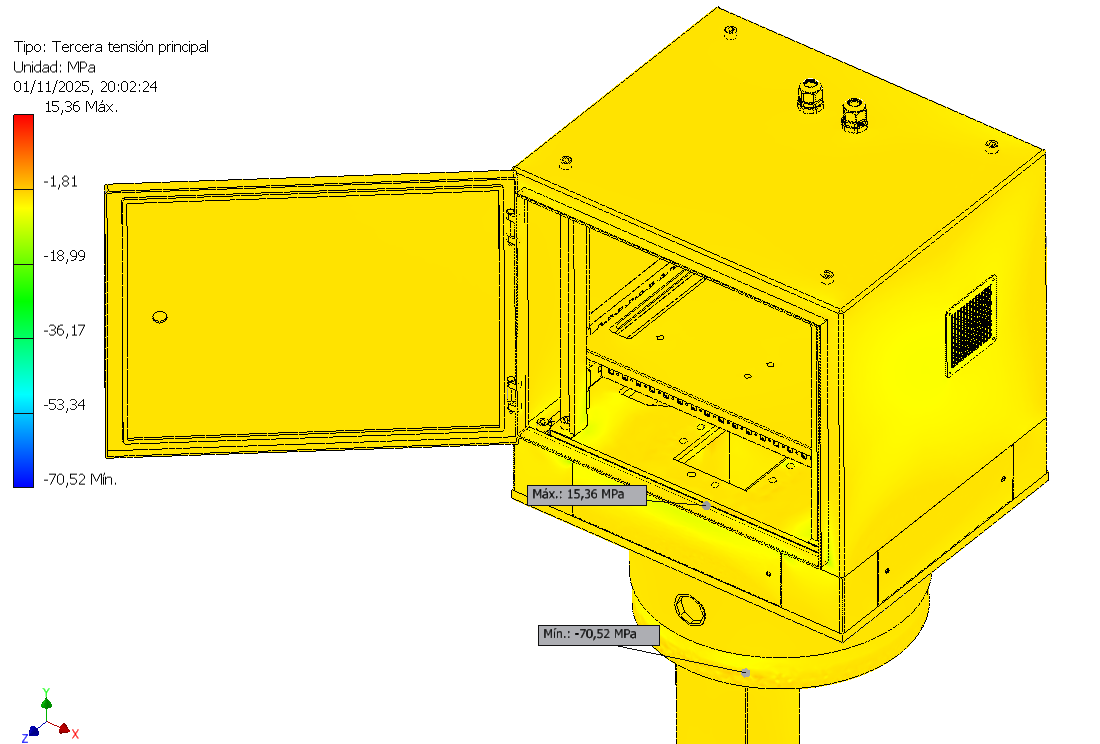
\includegraphics[width=0.92\linewidth,height=0.62\textheight,keepaspectratio]{./media/image141.png}
\captionof*{figure}{\small\itshape Figura 90. Distribución de tercera tensión principal}
\addcontentsline{lof}{figure}{Figura 90. Distribución de tercera tensión principal}
\label{fig:90}
\end{center}

El análisis revela:

\begin{itemize}
\item
  \textbf{Valor máximo de compresión:} \textbf{-70.52 MPa} localizado en la parte frontal inferior del sistema de vigilancia (zona de conexión aro-poste)
\item
  \textbf{Valor máximo de tracción:} \textbf{15.36 MPa} localizado en la parte frontal de la base del rack
\end{itemize}

La distribución de tensiones de compresión muestra concentraciones en tres zonas estructurales críticas:

\textbf{Zona 1 - Sistema de vigilancia inferior (máxima compresión):}

La compresión máxima de -70.52 MPa se localiza en la cara frontal de la conexión entre el aro estructural del sistema de vigilancia y el poste. Este valor representa el esfuerzo de compresión complementario a la tracción de 39.63 MPa observada en la primera tensión principal en el lado opuesto de la misma sección, comportamiento típico de elementos sometidos a flexión donde las fibras extremas experimentan esfuerzos de signo opuesto. La magnitud relativamente alta de esta compresión se debe a la combinación del momento flector generado por el peso del sistema de visión (11.3 kg) en voladizo y la carga lateral de viento sobre el área expuesta del aro circular. A pesar de alcanzar -70.52 MPa, este valor representa solamente el 36.5\% del límite elástico del aluminio 5052-H32 (193 MPa), confirmando operación segura en rango elástico.

\textbf{Zona 2 - Base frontal del rack (tracción moderada):}

La zona de tracción de 15.36 MPa en la parte frontal de la base del rack se genera por la flexión de los perfiles verticales del rack cuando soportan las cargas gravitatorias de los componentes pesados (UPS 3.5 kg, SMPS 1.2 kg) posicionados en los niveles superiores. La ubicación frontal de esta tensión indica que los perfiles experimentan flexión hacia adelante (hacia la puerta del gabinete) bajo la acción combinada del peso de componentes y la presión de viento sobre el gabinete que tiende a empujar todo el conjunto hacia atrás. Este valor de 15.36 MPa es bajo, representando menos del 8\% del límite elástico del aluminio, confirmando que los perfiles de 30\ensuremath{\times}30 mm proporcionan rigidez más que suficiente.

\textbf{Zona 3 - Perfiles verticales del rack (compresión distribuida):}

Los perfiles verticales del rack muestran compresión moderada distribuida a lo largo de su longitud, particularmente en las esquinas donde se concentran los puntos de apoyo de los componentes pesados. Esta compresión confirma la transferencia efectiva de cargas gravitatorias desde los niveles superiores (donde están UPS y SMPS) hacia la base del rack y finalmente hacia el gabinete. La distribución uniforme de la compresión (tonalidad amarilla consistente en la imagen) indica que no hay concentraciones locales excesivas, validando el diseño de distribución de cargas del rack mediante bandejas perforadas y perfiles estructurales.

\textbf{Verificación contra pandeo local:}

El valor máximo de compresión de -70.52 MPa debe verificarse contra el riesgo de pandeo local en las paredes del perfil tubular del poste. Para perfiles tubulares rectangulares sometidos a compresión, el pandeo local se evalúa mediante la relación ancho-espesor según criterios de diseño estructural AISC.

La relación ancho-espesor del perfil cuadrado 130\ensuremath{\times}130\ensuremath{\times}10 mm, donde t=10 mm es el espesor de pared, y b=130 mm es el ancho de la cara, es:

\begin{centeredmath}
\lambda = b/t\  = 13\quad \ \ \ \ \ \ \ \ \ \ \ \ \ \ \ \ \ \ \ \ \ \ \ \ \ \ \ \ \ \ \ \ \ \ \ \ \ \ \ \ \ \ \ \ \ \ \ \ \ \ \ \ \ \ \ \ \ \ \ \ \ \ \ (1)
\end{centeredmath}

Para elementos en compresión uniforme (paredes de perfiles tubulares), el límite para clasificación como sección compacta (sin riesgo de pandeo local antes de alcanzar límite elástico) según AISC es:

\begin{centeredmath}
\ \ \ \ \ \ \ \ \ \ \ \ \ \ \ \ \ \ \ \ \ \ \ \ \ \ \ \ \lambda p\  = \ 1.12\  \times \ \sqrt{}(E/fy)\  = \ 1.12\  \times \ \sqrt{}(200,000/250)\  = \  \approx \ 31.7\quad \ \ \ \ \ \ \ \ \ \ \ \ \ \ \ (2)
\end{centeredmath}

Donde E es el módulo de elasticidad del acero (200,000 MPa) y fy es el límite elástico del acero A36 (250 MPa).

Como \ensuremath{\lambda} = 13 \textless{} \ensuremath{\lambda}p = 31.7, el perfil se clasifica como sección compacta lo que significa que las paredes del perfil alcanzarán el límite elástico del material (250 MPa) antes de experimentar pandeo local. Por lo tanto, el criterio de falla relevante es el límite elástico, no el pandeo.

El factor de seguridad respecto al límite elástico es:

\begin{centeredmath}
\ \ \ \ \ \ \ \ \ \ \ \ \ \ \ \ \ \ \ \ \ \ \ \ \ \ \ \ \ \ FS_{\text{Material}}\ = f_{y}\ /\ \sigma_{\text{compresión}} = 250\ MPa\ /\ 70.52\ MPa\  = \ 3.545\ \qquad (3)
\end{centeredmath}

La compresión máxima de -70.52 MPa representa solamente el 28.2\% del límite elástico del acero A36.

\subsection{Análisis de desplazamientos}\label{anuxe1lisis-de-desplazamientos}

El análisis de desplazamientos verifica que las deformaciones del sistema permanezcan dentro de límites aceptables que no comprometan funcionalidad ni generen incomodidad visual o preocupación pública.

\begin{center}
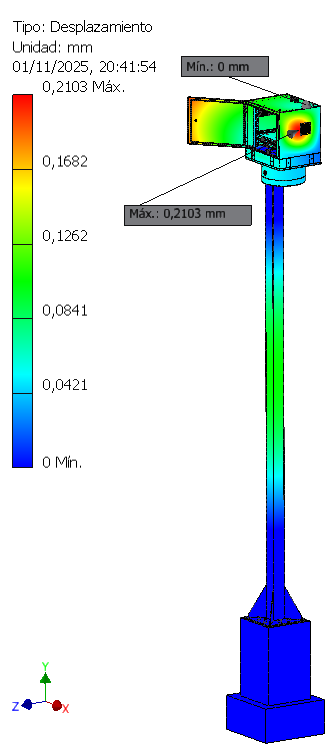
\includegraphics[width=0.92\linewidth,height=0.62\textheight,keepaspectratio]{./media/image61.png}
\captionof*{figure}{\small\itshape Figura 91. Campo de desplazamientos totales del sistema}
\addcontentsline{lof}{figure}{Figura 91. Campo de desplazamientos totales del sistema}
\label{fig:91}
\end{center}

\begin{center}
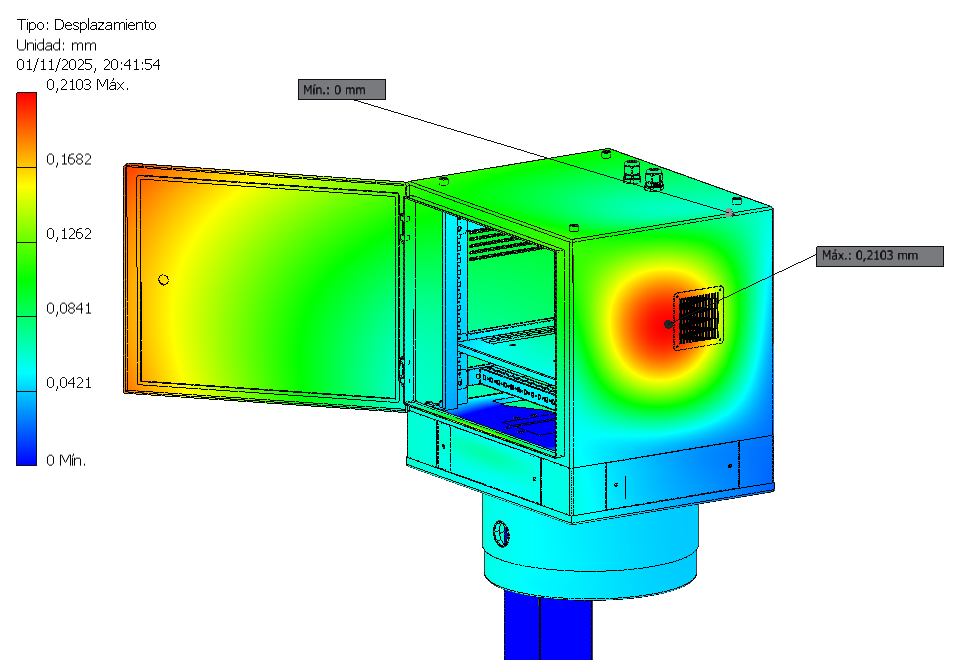
\includegraphics[width=0.92\linewidth,height=0.62\textheight,keepaspectratio]{./media/image99.png}
\captionof*{figure}{\small\itshape Figura 92. Desplazamientos en el Gabinete}
\addcontentsline{lof}{figure}{Figura 92. Desplazamientos en el Gabinete}
\label{fig:92}
\end{center}

Los resultados muestran:

\begin{itemize}
\item
  \textbf{Desplazamiento máximo:} \textbf{0.2103 mm} localizado en la zona lateral del gabinete
\item
  \textbf{Desplazamiento mínimo:} \textbf{0 mm} en la base del poste (zona de empotramiento)
\end{itemize}

\textbf{Interpretación de desplazamientos}

La distribución de desplazamientos muestra un gradiente progresivo desde la base empotrada (color azul oscuro, 0 mm) hasta las zonas superiores del gabinete. La escala cromática revela:

\textbf{Zona azul oscura (base del poste):} Desplazamiento nulo (0 mm) confirmando el empotramiento efectivo de la placa base en la zapata de cimentación.

\textbf{Zona azul-cyan (sistema de vigilancia inferior y parte baja del poste):} Desplazamientos mínimos, indicando alta rigidez en la zona de conexión aro estructural-poste.

\textbf{Zona verde-amarilla (gabinete y parte media del poste):} Desplazamientos intermedios que aumentan gradualmente con la altura.

\textbf{Zona naranja-roja (esquinas superiores del gabinete):} Desplazamiento máximo de 0.2103 mm en las zonas más alejadas del empotramiento, comportamiento esperado en estructuras en voladizo.

El desplazamiento lateral máximo de \textbf{0.2103 mm} es extremadamente pequeño y representa una deflexión prácticamente imperceptible. Es importante contextualizar que este desplazamiento se produce bajo carga de viento extrema de 1.5 kPa (175 km/h), condición que excede significativamente los eventos de viento típicos en Lima Metropolitana.

Bajo presión de viento de diseño nominal de 1.0 kPa (145 km/h, tiempo de retorno 50 años), los desplazamientos se reducirían proporcionalmente a aproximadamente 0.14 mm.

Este valor nominal representa una deflexión completamente imperceptible visualmente.

\subsection{Análisis de factor de seguridad}\label{anuxe1lisis-de-factor-de-seguridad}

El software Autodesk Inventor calcula el factor de seguridad en cada elemento del modelo, proporcionando visualización cromática que identifica zonas críticas.

\begin{center}
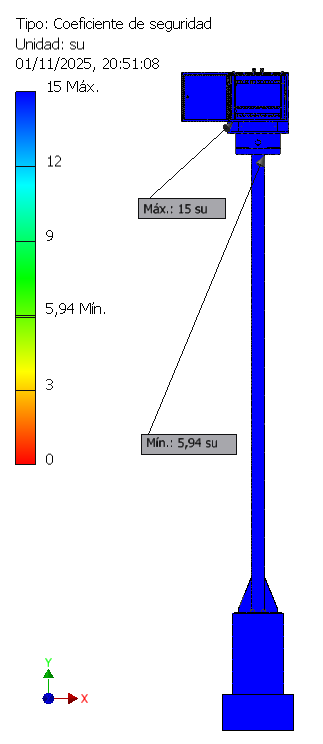
\includegraphics[width=0.92\linewidth,height=0.62\textheight,keepaspectratio]{./media/image130.png}
\captionof*{figure}{\small\itshape Figura 93. Distribución de factor de seguridad en el sistema}
\addcontentsline{lof}{figure}{Figura 93. Distribución de factor de seguridad en el sistema}
\label{fig:93}
\end{center}

\begin{center}
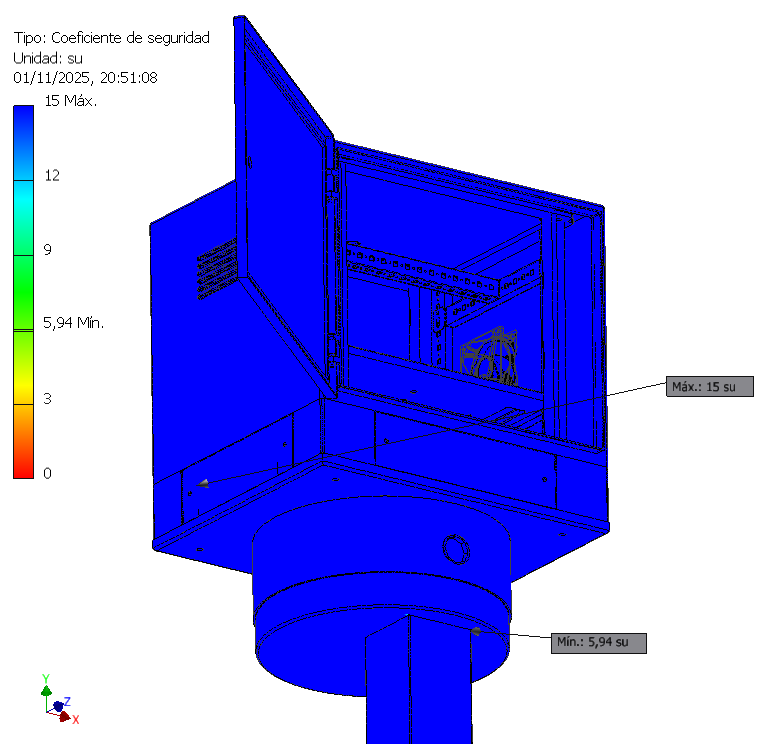
\includegraphics[width=0.92\linewidth,height=0.62\textheight,keepaspectratio]{./media/image1.png}
\captionof*{figure}{\small\itshape Figura 94. Factor de Seguridad enfocado en el Gabinete}
\addcontentsline{lof}{figure}{Figura 94. Factor de Seguridad enfocado en el Gabinete}
\label{fig:94}
\end{center}

Los resultados del análisis muestran:

\begin{itemize}
\item
  \textbf{Factor de seguridad mínimo:} \textbf{5.94} localizado en la zona de conexión entre el sistema de vigilancia inferior y el poste
\item
  \textbf{Factor de seguridad en la mayor parte del sistema:} \ensuremath{\geq} 15 (tonalidad azul uniforme en gabinete, rack y poste)
\end{itemize}

\textbf{Interpretación de factores de seguridad}

La distribución cromática del factor de seguridad revela que prácticamente todo el sistema (tonalidad azul uniforme) opera con factores de seguridad superiores a 15, lo que indica que las tensiones actuantes son al menos 15 veces menores que los límites elásticos de los materiales. Esta situación confirma un diseño conservador.

\textbf{Zona de factor de seguridad mínimo (FS = 5.94):}

El factor de seguridad mínimo de 5.94 se localiza en la zona de transición entre el aro estructural del sistema de vigilancia y el perfil tubular del poste (visible en tonalidad verde-cyan en la imagen). Esta reducción localizada del factor de seguridad se debe a la concentración de esfuerzos generada por tres factores concurrentes:

\begin{enumerate}
\def\labelenumi{\arabic{enumi}.}
\item
  \textbf{Discontinuidad geométrica:} El cambio brusco de sección transversal desde el perfil cuadrado del poste hacia la geometría circular del aro actúa como concentrador de esfuerzos, elevando las tensiones locales en la zona de transición.
\item
  \textbf{Carga en voladizo:} El peso del sistema de visión completo actuando en voladizo desde el eje del poste genera momento flector que se transfiere al poste en esta conexión.
\item
  \textbf{Presión lateral de viento:} La carga de viento de 1.5 kPa actuando sobre el área expuesta del aro circular amplifica el momento flector en la zona de unión.
\end{enumerate}

A pesar de ser el punto más esforzado del sistema, el factor de seguridad de 5.94 es satisfactorio y conservador para estructuras de soporte de equipamiento urbano considerando:

\textbf{1. Naturaleza de las cargas:}

Las cargas de viento son cíclicas y pueden inducir fatiga en el largo plazo. La normativa internacional para estructuras metálicas sometidas a cargas cíclicas recomienda factores de seguridad mínimos de 3.0 para prevenir degradación por fatiga. El factor de seguridad de 5.94 proporciona un margen adicional sustancial sobre este requisito mínimo, garantizando vida útil superior a 15 años sin riesgo de falla por fatiga.

\textbf{2. Incertidumbres del modelo:}

El análisis FEA asume condiciones ideales: geometría perfecta sin tolerancias de fabricación, propiedades de material homogéneas sin variaciones locales, y soldaduras de calidad perfecta sin defectos internos. El factor de seguridad de 5.94 compensa estas imperfecciones inevitables de fabricación y montaje, proporcionando robustez ante variaciones reales de calidad constructiva.

\textbf{3. Cargas no consideradas:}

El análisis estático no incluye efectos dinámicos como ráfagas de viento impulsivas que pueden generar picos de carga instantáneos superiores a la presión media, vibraciones de tráfico vehicular cercano transmitidas a través de la zapata, o impactos accidentales durante el mantenimiento. El margen de seguridad adicional proporciona robustez ante estos eventos no modelados explícitamente.

\section{Listado consolidado de planos mecánicos}\label{listado-consolidado-de-planos-mecuxe1nicos}

Compendio de los planos técnicos generados durante el proceso de diseño, organizados por subsistemas en Anexos.

\chapter{DISEÑO DE LA ETAPA DE CONTROL}\label{capuxedtulo-6-diseuxf1o-de-la-etapa-de-control}

\section{Desarrollo de algoritmos de control adaptativo}\label{desarrollo-de-algoritmos-de-control-adaptativo}

El sistema de control adaptativo inteligente propuesto para la red semafórica vial de Lima Metropolitana se fundamenta en la necesidad crítica de superar las limitaciones inherentes a los sistemas de control de tiempo fijo y programables que actualmente operan en la mayoría de intersecciones de la ciudad. Los sistemas convencionales, basados en temporizadores preestablecidos que no responden a las condiciones reales del tráfico, generan ineficiencias sistémicas que se manifiestan en tiempos de espera excesivos, congestión vehicular crónica y desperdicio de capacidad vial durante periodos de baja demanda.

En esta tesis, el control difuso local constituye el núcleo de decisión validable del módulo propuesto, debido a que permite trabajar con variables interpretables como cola, flujo, velocidad e índice de congestión. Los componentes de aprendizaje por refuerzo y predicción CNN-LSTM se presentan como capas de optimización y extensión futura, útiles para coordinación global y análisis predictivo, pero no como sustitutos inmediatos del controlador semafórico certificado. Esta delimitación mantiene la propuesta dentro de un alcance técnico realista para una tesis de titulación.

\subsection{Arquitectura del Sistema}\label{arquitectura-del-sistema}

El sistema integra tres componentes que operan sinérgicamente:

\textbf{1. Subsistema de Percepción mediante Visión por Computadora}

Implementa algoritmos de detección de objetos basados en redes neuronales convolucionales (específicamente YOLO) que procesan video en tiempo real capturado por la cámara domo DS-2CE57H0T-VPITF instalada en el centro de la intersección. Este subsistema extrae información cuantitativa sobre el estado del tráfico, incluyendo conteo vehicular, estimación de velocidades promedio, detección de colas vehiculares y clasificación de vehículos (vehículos de emergencias).

\textbf{2. Subsistema de decisión local y optimización global}

La decisión inmediata se basa en lógica difusa, ya que permite manejar la incertidumbre inherente a las mediciones sensoriales y proporciona respuestas interpretables para operadores humanos. Sobre esta capa se plantea un motor de aprendizaje por refuerzo como módulo experimental de coordinación global, entrenado en simulación y orientado a recomendar ajustes de red bajo condiciones previamente validadas.

\textbf{3. Infraestructura de Comunicación en la Nube}

Facilita la coordinación entre múltiples intersecciones mediante procesamiento centralizado de datos agregados, permitiendo análisis de propagación de congestión y olas verdes coordinadas. La plataforma Microsoft Azure ejecuta procesamiento de datos para identificar patrones históricos y generar recomendaciones de control global, las cuales deben conservar límites operativos y validación local antes de su aplicación.

\section{Sistema de Control Local}\label{sistema-de-control-local}

El control local opera de manera autónoma en cada intersección \(I_{p}\), procesando información sensorial en tiempo real capturada por la cámara domo para generar decisiones de control inmediatas basadas en las condiciones actuales del tráfico.

\subsection{Función de Orientación de Cámara}\label{funciuxf3n-de-orientaciuxf3n-de-cuxe1mara}

Cada intersección \(I_{p}\) cuenta con una cámara domo que alterna entre dos vistas perpendiculares para capturar el estado del tráfico en los cuatro accesos de la intersección:

\begin{itemize}
\item
  \textbf{Vista Norte--Sur (NS)}: Visualiza carriles Norte y Sur
\item
  \textbf{Vista Este--Oeste (EO)}: Visualiza carriles Este y Oeste
\end{itemize}

El estado de observación de la cámara en el instante t se representa mediante la función de máscara:

\begin{centeredmath}
CamMask(I_{p},t) =
\begin{cases}
1, & \text{si la cámara apunta hacia Norte--Sur}\\[2pt]
0, & \text{si la cámara apunta hacia Este--Oeste}
\end{cases}
\end{centeredmath}

Esta función determina qué grupo de carriles (NS o EO) se encuentran visibles para el cálculo de métricas en un instante dado, controlando la actualización de las matrices de estado local.

\subsection{Variables de Entrada del Sistema Local}\label{variables-de-entrada-del-sistema-local}

Las variables de entrada se calculan en tiempo real a partir del procesamiento de video mediante YOLO y ByteTrack, y se organizan en vectores por dirección que se actualizan según la orientación de la cámara.

\textbf{Función de Cola vehicular - Conteo de vehículos Detenidos}

Cuantifica el número de vehículos prácticamente inmóviles en cada carril, indicando acumulación de demanda en el semáforo.

\begin{centeredmath}
StoppedCount(l,t) = \sum_{v \in V(l,t)}\delta[v]
\end{centeredmath}

donde la función indicadora se define como:

\begin{centeredmath}
\delta[v] =
\begin{cases}
1, & \text{si } velocidad(v) < \varepsilon\\[2pt]
0, & \text{caso contrario}
\end{cases}
\end{centeredmath}

La actualización vectorial controlada por la orientación de cámara es:

\begin{centeredmath}
SC_{p}(t) =
\begin{cases}
\left[\, SC_{N},\ SC_{S},\ 0,\ 0 \,\right], & CamMask(I_{p},t) = 1\\[2pt]
\left[\, 0,\ 0,\ SC_{E},\ SC_{O} \,\right], & CamMask(I_{p},t) = 0
\end{cases}
\end{centeredmath}

Variables:

\begin{itemize}
\item
  \(StoppedCount(l,t):\) número de vehículos detenidos en el carril l al tiempo t.
\item
  \(V(l,t):\) conjunto de vehículos detectados en l en t.
\item
  \(\delta\lbrack v\rbrack\): función indicadora que vale 1 si el vehículo v está detenido.
\item
  \(velocidad\ (v)\): velocidad instantánea del vehículo v (ByteTrack).
\item
  \(\varepsilon\): umbral de velocidad para considerar un vehículo detenido.
\item
  \(SC_{N},SC_{S},SC_{E},SC_{O}:\) conteo de vehículos detenidos por dirección.
\end{itemize}

\textbf{Función Velocidad Promedio vehicular}

Evalúa la fluidez del tráfico considerando únicamente vehículos en movimiento, excluyendo los detenidos.

\begin{centeredmath}
V_{avg\ }(l,t)\  = \frac{1}{N_{mov}(l,t)}\sum_{v \in V_{mov}(l,t)}^{}velocidad\ (v)
\end{centeredmath}

Donde:

\begin{centeredmath}
V_{mov}(l,t) = \{ v \in V(l,t)\ :\ velocidad(v) \geq \varepsilon\},\ N_{mov}(l,t) = \left| V_{mov}(l,t) \right|\
\end{centeredmath}

Para que la variable quede definida en todo escenario se adoptan dos convenciones de borde: si no hay vehículos en el carril (\(N_{total} = 0\)), se asigna \(V_{avg} = V_{MAX}\), pues la ausencia de demanda equivale operativamente a flujo libre; si hay vehículos pero todos están detenidos (\(N_{total} > 0 \land N_{mov} = 0\)), se asigna \(V_{avg} = 0\), el caso de máxima retención. Estas convenciones evitan indeterminaciones del promedio y garantizan que los índices derivados (ICV, PI) interpreten correctamente tanto la vía vacía como la vía bloqueada.

Actualización vectorial:

\begin{centeredmath}
V_{avg,p}(t) =
\begin{cases}
\left[\, V_{N},\ V_{S},\ 0,\ 0 \,\right], & CamMask(I_{p},t) = 1\\[2pt]
\left[\, 0,\ 0,\ V_{E},\ V_{O} \,\right], & CamMask(I_{p},t) = 0
\end{cases}
\end{centeredmath}

Variables:

\begin{itemize}
\item
  \(V_{avg}(l,t):\) velocidad promedio en el carril l.
\item
  \(N_{mov}(l,t):\) número de vehículos en movimiento.
\item
  \(V_{mov}(l,t)\): conjunto de vehículos con velocidad \ensuremath{\geq} \ensuremath{\varepsilon}.
\item
  \(V_{N},V_{S},V_{E},V_{O}:\) velocidades promedio por dirección.
\end{itemize}

\textbf{Función Flujo Vehicular}

Mide la tasa de salida de vehículos de la intersección, útil para estimar capacidad y eficiencia operativa instantánea.

\begin{centeredmath}
q(l,t) = \frac{N_{cross}(l,\ t_{0},\ t)}{t\  - \ t_{0}}
\end{centeredmath}

Donde \(N_{cross}(l,\ t_{0},\ t)\) es el número de vehículos que cruzaron una línea de conteo virtual en el carril l entre los tiempos t0 y t, calculado con YOLO.

Actualización vectorial:

\begin{centeredmath}
q_{p}(t) =
\begin{cases}
\left[\, q_{N},\ q_{S},\ 0,\ 0 \,\right], & CamMask(I_{p},t) = 1\\[2pt]
\left[\, 0,\ 0,\ q_{E},\ q_{O} \,\right], & CamMask(I_{p},t) = 0
\end{cases}
\end{centeredmath}

Variables:

\begin{itemize}
\item
  \(q(l,t)\): flujo vehicular (vehículos por unidad de tiempo)
\item
  \(N_{cross}(l,\ t_{0},\ t)\): número de vehículos que cruzan la línea de salida.
\item
  t0\hspace{0pt}, t: tiempos inicial y actual del intervalo de medición.
\end{itemize}

\textbf{Función de Densidad Vehícular}

Refleja el nivel de ocupación espacial de cada carril. Una alta densidad implica congestión.

\begin{centeredmath}
k(l,t) = \frac{N_{total}(l,\ t)}{L_{efectiva}}
\end{centeredmath}

donde:

\begin{itemize}
\item
  \(Ntotal(l,t) = \mid V(l,t) \mid :\) número total de vehículos detectados en el carril l.
\item
  \(L_{efectiva}:\) longitud efectiva del área visible en metros.
\end{itemize}

Actualización vectorial:

\begin{centeredmath}
k_{p}(t) =
\begin{cases}
\left[\, k_{N},\ k_{S},\ 0,\ 0 \,\right], & CamMask(I_{p},t) = 1\\[2pt]
\left[\, 0,\ 0,\ k_{E},\ k_{O} \,\right], & CamMask(I_{p},t) = 0
\end{cases}
\end{centeredmath}

A diferencia del modelo clásico de la relación fundamental del tráfico \(k = q/V_{avg}\), esta formulación calcula la densidad espacialmente, lo cual resulta más adecuado para sistemas de visión por computadora donde se cuenta directamente el número de vehículos en un área conocida.

\textbf{Función Detección de Vehículos de Emergencia}

Identifica la presencia de ambulancias y vehículos de bomberos para activar protocolos de priorización.

\begin{centeredmath}
EV(l,t) = \sum_{v \in V(l,t)}\delta_{emg}[v,t]
\end{centeredmath}

donde la función indicadora se define como:

\begin{centeredmath}
\delta_{emg}[v,t] =
\begin{cases}
1, & \text{si } class(v) \in C_{emg} \ \land\ confidence(v) \geq \tau_{EV}\\[2pt]
0, & \text{caso contrario}
\end{cases}
\end{centeredmath}

Variables:

\begin{itemize}
\item
  \(EV(l,t)\): número de vehículos de emergencia detectados en la intersección \(I_{p}\), dirección \(d \in \{N, S, E, O\}\), en el tiempo \(t\).
\item
  \(V(l,t)\): conjunto de vehículos detectados en el carril.
\item
  \(class(v)\): clase predicha por YOLO para el objeto \(v\).
\item
  \(C_{emg} = \{\text{ambulancias},\ \text{bomberos}\}\): conjunto de clases de emergencia.
\item
  \(confidence(v)\): puntaje de confianza de la detección, en el rango \([0,1]\).
\item
  \(\tau_{EV}\): umbral mínimo de confianza para validar una detección de emergencia (se adopta \(\tau_{EV} = 0.85\) para minimizar falsos positivos, dado el alto impacto de una activación errónea de prioridad).
\end{itemize}

\textbf{Seguimiento Continuo y Predicción de Trayectoria}

Una vez detectado un vehículo de emergencia, el sistema entra en modo de seguimiento activo mediante ByteTrack, registrando su estado completo:

\begin{centeredmath}
ev_{state}(v,t) = \left[\, pos_{x}(v,t),\ pos_{y}(v,t),\ vel_{x}(v,t),\ vel_{y}(v,t),\ DIR_{inicial}(v,t),\ DIR_{salida}(v,t) \,\right]
\end{centeredmath}

Donde:

\begin{itemize}
\item
  \(pos_{x},\ pos_{y}\): posición del centroide (coordenadas de imagen calibradas a metros mediante homografía).
\item
  \(vel_{x},\ vel_{y}\): componentes de velocidad en los ejes \(x\), \(y\) (estimadas por ByteTrack).
\item
  \(DIR_{inicial}(v,t)\): dirección de llegada, \(\in \{N, S, E, O\}\).
\item
  \(DIR_{salida}(v,t)\): dirección de salida del campo visual de la cámara.
\end{itemize}

\textbf{Control Reactivo de CamMask basado en Posición del EV}

El sistema implementa un mecanismo de control reactivo automático de la orientación de cámara específicamente diseñado para mantener la visibilidad continua de vehículos de emergencia (ambulancias, vehículos de bomberos) durante su tránsito por la intersección.

Para mantener visibilidad del vehículo de emergencia, se definen zonas de activación crítica que disparan el giro automático de la cámara:

\begin{centeredmath}
Zone(I_{p}) = \{\, Z_{NS \rightarrow EO},\ Z_{EO \rightarrow NS} \,\}
\end{centeredmath}

Para cada intersección I\ensuremath{_{p}}, se definen dos zonas geométricas complementarias que activan el cambio automático de orientación de la cámara domo. Estas zonas están calibradas en el sistema de coordenadas cartesianas del plano de la intersección, donde (xc, yc) representa el centroide geométrico de la intersección y R define el radio de cobertura efectiva de la cámara:

\begin{centeredmath}
Z_{NS \rightarrow EO} = \{\,(x,y) : R_{trigger} < \left| x - x_{c} \right| < R \,\}
\end{centeredmath}

\begin{centeredmath}
Z_{EO \rightarrow NS} = \{\,(x,y) : R_{trigger} < \left| y - y_{c} \right| < R \,\}
\end{centeredmath}

El parámetro \(R_{trigger}\) representa el umbral de distancia que activa el cambio de orientación. Cuando \(Pos(v_{EV})\  \in \ Zone(I_{p})\) se actualiza automáticamente:

\begin{centeredmath}
CamMask(I_{p},\ t) \leftarrow 1 - CamMask(I_{p},\ t)
\end{centeredmath}

Este mecanismo reactivo resuelve el problema fundamental de la cámara de vista única en intersecciones cruciformes: sin control automático, un vehículo de emergencia que se aproxima por el Norte sería visible inicialmente, pero al ingresar a la intersección y girar hacia el Este, saldría del campo visual si la cámara mantiene la orientación Norte--Sur.

\subsection{Índice de Congestión Vehicular Local (ICV)}\label{uxedndice-de-congestiuxf3n-vehicular-local-icv}

El ICV integra todas las variables de tráfico en un índice sintético continuo normalizado en {[}0,1{]} que representa el nivel de congestión de cada carril. Este índice facilita la interpretación del estado del tráfico y sirve como entrada compuesta al algoritmo de control.

\begin{centeredmath}
ICV(l,t) =
\begin{cases}
0, & \text{si } N_{total}(l,t) = 0\\[6pt]
w_{1}\,\dfrac{SC(l,t)}{SC_{MAX}} + w_{2}\left(1 - \dfrac{V_{avg}(l,t)}{V_{MAX}}\right) + w_{3}\,\dfrac{k(l,t)}{k_{MAX}} + w_{4}\left(1 - \dfrac{q(l,t)}{q_{MAX}}\right), & \text{si } N_{total}(l,t) > 0
\end{cases}
\end{centeredmath}

La compuerta por demanda (\(ICV \doteq 0\) cuando no hay vehículos) es necesaria porque un flujo bajo es ambiguo por sí solo: una vía vacía y una vía bloqueada producen ambas \(q \approx 0\), pero solo la segunda está congestionada. Al condicionar el índice a la presencia de vehículos detectados, el término \(1 - q/q_{MAX}\) mide \emph{demanda insatisfecha} (vehículos presentes que no logran cruzar) y no penaliza la simple ausencia de demanda. Esta distinción es directamente observable por el sistema de visión, pues \(N_{total}\) proviene del conteo YOLO del propio carril.

Normalización por carril:

\begin{centeredmath}
ICV_{norm}(l,t) = \frac{ICV(l,t) - ICV_{MIN}}{ICV_{MAX} - ICV_{MIN}}
\end{centeredmath}

Variables:

\begin{itemize}
\item
  \(w_{1}, w_{2}, w_{3}, w_{4}\): pesos de influencia. Como configuración inicial se adopta \(w_{1}=0.35\), \(w_{2}=0.25\), \(w_{3}=0.25\), \(w_{4}=0.15\), priorizando la cola detenida como el indicador más directo de demanda insatisfecha. Estos valores no son arbitrarios en el diseño final: se calibran mediante búsqueda en malla sobre el simplex \(\sum w_{i}=1\) en el entorno SUMO del Capítulo 7, tomando como función objetivo la minimización del tiempo promedio de espera por vehículo --- la medida de demora que el HCM emplea como criterio de nivel de servicio en intersecciones semaforizadas. De este modo, el ICV actúa como aproximación en tiempo real de la demora, que es la métrica de validación primaria del sistema.
\end{itemize}

Restricción de convexidad:

\begin{centeredmath}
\sum_{i = 1}^{4}w_{i} = 1, \qquad w_{i} \geq 0
\end{centeredmath}

Esta restricción garantiza que el ICV sea una combinación convexa de términos individualmente acotados en \([0,1]\), por lo que el índice resultante también queda acotado en \([0,1]\) sin necesidad de re-escalamiento posterior.

\begin{itemize}
\item
  \(SC(l,t):\) longitud de cola (número de vehículos detenidos o distancia ocupada).
\item
  \(V_{avg}(l,t)\): velocidad promedio del flujo vehicular.
\item
  \(k(l,t)\): densidad vehicular (vehículos por unidad de longitud).
\item
  \(q(l,t)\): flujo vehicular (vehículos por unidad de tiempo).
\end{itemize}

Actualización vectorial del ICV:

\begin{centeredmath}
ICV_{p}(t) =
\begin{cases}
\left[\, ICV_{N},\ ICV_{S},\ 0,\ 0 \,\right], & CamMask(I_{p},t) = 1\\[2pt]
\left[\, 0,\ 0,\ ICV_{E},\ ICV_{O} \,\right], & CamMask(I_{p},t) = 0
\end{cases}
\end{centeredmath}

Cabe resaltar que para el ICV global no se realizará el normalizado en esta parte, sino posteriormente junto con la normalización de la matriz de estado local.

\subsection{Parámetro de Intensidad (PI)}\label{paruxe1metro-de-intensidad-pi}

Cuantifica la relación entre la fluidez del tráfico (representada por la velocidad promedio) y el nivel de acumulación vehicular (representado por la longitud de cola). Este indicador permite detectar situaciones críticas donde la velocidad disminuye mientras la acumulación aumenta, reflejando un estado de congestión inminente.

\begin{centeredmath}
PI(l,t) = \frac{V_{avg}(l,t) + \delta}{SC(l,t) + \delta}
\end{centeredmath}

donde \(\delta\) es una pequeña constante de regularización (se adopta \(\delta = 0.1\)) que evita la división entre cero cuando la cola es nula y mantiene la estabilidad numérica en condiciones de flujo libre. Dado que tanto \(V_{avg}\) como \(SC\) ingresan normalizados a \([0,1]\), el cociente crudo varía en un rango muy asimétrico (desde \(\delta/(1+\delta)\) hasta \((1+\delta)/\delta\)), por lo que una normalización lineal comprimiría la mayoría de los estados operativos cerca de cero. Para evitarlo, el PI se acota al rango \([0,1]\) mediante la transformación racional:

\begin{centeredmath}
PI_{norm}(l,t) = \frac{PI(l,t)}{1 + PI(l,t)} = \frac{V_{avg}(l,t) + \delta}{V_{avg}(l,t) + SC(l,t) + 2\delta}
\end{centeredmath}

Esta transformación es estrictamente creciente y reparte el rango de salida de forma equilibrada: cuando velocidad y cola se igualan (\(V_{avg} = SC\)) resulta \(PI_{norm} = 0.5\), el punto de equilibrio entre movilidad y retención; el flujo libre puro (\(V_{avg}=1,\ SC=0\)) produce \(PI_{norm} \approx 0.92\) y el bloqueo total (\(V_{avg}=0,\ SC=1\)) produce \(PI_{norm} \approx 0.08\). Esta propiedad da significado físico directo a los umbrales de los conjuntos difusos definidos más adelante (0.3 / 0.5 / 0.8): el valor 0.5 separa exactamente los estados donde domina la movilidad de aquellos donde domina la acumulación. Junto con las convenciones de borde de \(V_{avg}\) (vía vacía \(\rightarrow PI_{norm}\) alto, vía bloqueada \(\rightarrow PI_{norm}\) bajo), el indicador queda definido y es interpretable en todo el espacio de estados. En adelante, toda referencia al PI transmitido o procesado alude a \(PI_{norm}\).

La lógica se fundamenta en la interacción inversa entre velocidad y acumulación, pues a medida que el tráfico se vuelve más denso, las colas (SC) aumentan y la velocidad promedio (Vavg) disminuye. Por tanto el cociente \(\frac{V_{avg}}{SC}\ \)disminuye, reflejando condiciones de congestión. En cambio, cuando la vía está despejada, la velocidad promedio es alta y la acumulación baja, generando un PI elevado que indica flujo eficiente.

De esta manera, el PI actúa como un índice de eficiencia instantánea del carril, integrando dos aspectos complementarios del tráfico: movilidad (velocidad) y ocupación (cola). Además, al ser una magnitud adimensional y continua, facilita su incorporación en algoritmos de control difuso, donde puede emplearse como variable auxiliar de ajuste dinámico.

\textbf{Aplicación en el Sistema de Control Global:}

El valor del PI se utiliza por el sistema de procesamiento en Azure para dos propósitos fundamentales:

\begin{enumerate}
\def\labelenumi{\arabic{enumi}.}
\item
  \textbf{Modulación adaptativa de fases verdes:} El sistema de control global analiza el PI de todos los carriles para ajustar dinámicamente la duración de las fases verdes mediante reglas difusas implementadas en el motor de decisión:

  \begin{enumerate}
  \def\labelenumii{\alph{enumii}.}
  \item
    \emph{Si PI es bajo \ensuremath{\rightarrow} aumentar el tiempo verde en el carril afectado}, compensando la congestión y reduciendo la cola.
  \item
    \emph{Si PI es alto \ensuremath{\rightarrow} reducir el tiempo verde o mantener la sincronización actual}, priorizando otros flujos con menor eficiencia.
  \end{enumerate}
\item
  \textbf{Predicción de propagación de congestión:} Los modelos CNN-LSTM utilizan series temporales del PI junto con el ICV para anticipar situaciones de congestión en intersecciones vecinas antes de que se materialicen, permitiendo acciones preventivas de control coordinado.
\end{enumerate}

Actualización vectorial del PI:

\begin{centeredmath}
PI_{p}(t) =
\begin{cases}
\left[\, PI_{N},\ PI_{S},\ 0,\ 0 \,\right], & CamMask(I_{p},t) = 1\\[2pt]
\left[\, 0,\ 0,\ PI_{E},\ PI_{O} \,\right], & CamMask(I_{p},t) = 0
\end{cases}
\end{centeredmath}

El PI se transmite como parte de la matriz de estado local al sistema centralizado en Azure, donde se integra con datos de todas las intersecciones para optimización de red global.

En conjunto con el Índice de Congestión Vehicular (ICV), el PI favorece la capacidad del sistema para responder flexiblemente y anticipadamente ante variaciones en la demanda de tráfico, contribuyendo así a una gestión semafórica más eficiente, estable y equitativa entre los distintos sentidos de circulación.

Una visualización de todas estas variables locales se evidencia en la siguiente figura, donde se denota como se usan las principales variables locales, las 5 funciones de detección, para generar 2 funciones locales integradas las cuales nos brindan PI y ICV local. Figura 95.

\begin{center}
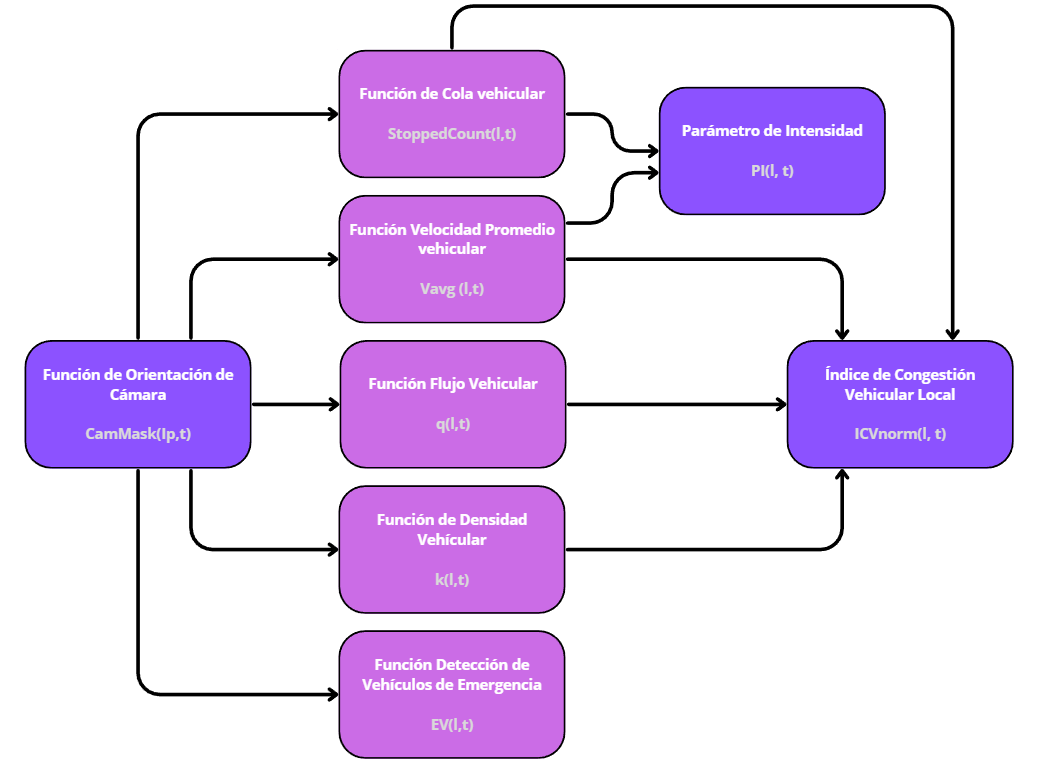
\includegraphics[width=0.92\linewidth,height=0.62\textheight,keepaspectratio]{./media/image95.png}
\captionof*{figure}{\small\itshape Figura 95. Relación de Variables Locales}
\addcontentsline{lof}{figure}{Figura 95. Relación de Variables Locales}
\label{fig:95}
\end{center}

\subsubsection{Matriz de estado local para transmisión}\label{matriz-de-estado-local-para-transmisiuxf3n}

La matriz de estado de la intersección \(I_{p}\) en el instante t consolida todas las variables de entrada normalizadas, que se transmite a la plataforma Azure para su procesamiento centralizado:
\begin{centeredmath}
X_{\text{local}}^{(p)}(t)=
\begin{bmatrix}
SC_N(t)\\
SC_S(t)\\
SC_E(t)\\
SC_O(t)\\
V_{\text{avg},N}(t)\\
V_{\text{avg},S}(t)\\
V_{\text{avg},E}(t)\\
V_{\text{avg},O}(t)\\
q_N(t)\\
q_S(t)\\
q_E(t)\\
q_O(t)\\
k_N(t)\\
k_S(t)\\
k_E(t)\\
k_O(t)\\
ICV_N(t)\\
ICV_S(t)\\
ICV_E(t)\\
ICV_O(t)\\
PI_N(t)\\
PI_S(t)\\
PI_E(t)\\
PI_O(t)\\
EV_N(t)\\
EV_S(t)\\
EV_E(t)\\
EV_O(t)
\end{bmatrix}
\in \mathbb{R}^{28}
\end{centeredmath}

Normalización:

\begin{centeredmath}
X_{norm} = \frac{X - X_{MIN}}{X_{MAX} - X_{MIN}}
\end{centeredmath}

La normalización se realiza para escalar todas las variables a un rango común, normalmente {[}0,1{]}, garantizando que magnitudes con diferentes unidades tengan una influencia comparable dentro del controlador adaptativo o difuso. En este caso, la normalización se efectúa por variable y no sobre el vector total, aplicando el proceso a cada componente de forma independiente:
\begin{centeredmath}
\begin{aligned}
X_{\text{local}}(p,t)
&=
\begin{bmatrix}
x_1(t)\\
x_2(t)\\
\vdots\\
x_{28}(t)
\end{bmatrix}
\Rightarrow
X_{\text{local,norm}}(p,t)
=
\begin{bmatrix}
\dfrac{x_1-x_{1,\min}}{x_{1,\max}-x_{1,\min}}\\
\dfrac{x_2-x_{2,\min}}{x_{2,\max}-x_{2,\min}}\\
\vdots\\
\dfrac{x_{28}-x_{28,\min}}{x_{28,\max}-x_{28,\min}}
\end{bmatrix}
\end{aligned}
\end{centeredmath}

Usar un único rango global para todo el vector sería incorrecto, ya que mezclará escalas heterogéneas y haría que las variables de menor magnitud (como indicadores lógicos o banderas de emergencia) queden prácticamente anuladas.

Para ejecutar correctamente este proceso se requieren dos matrices auxiliares:

\begin{itemize}
\item
  XMAX\hspace{0pt}: contiene los valores máximos esperados de cada variable.
\item
  XMIN\hspace{0pt}: contiene los valores mínimos correspondientes.
\end{itemize}

Estas matrices permiten calibrar dinámicamente los rangos máximos y mínimos si las condiciones del tráfico cambian, por ejemplo, durante horas pico o ante situaciones atípicas. De este modo, se mantiene la coherencia del modelo y se evita que el sistema pierda sensibilidad ante variaciones en las condiciones reales.

En cuanto a sus ventajas operativas, la normalización permite la uniformidad de escalas, impidiendo que variables con valores grandes dominen la respuesta del sistema y distorsionen el análisis global. También asegura la compatibilidad con métodos de control difuso o adaptativo, dado que estos algoritmos funcionan de manera más estable y precisa cuando las entradas se encuentran dentro de rangos acotados y comparables. Asimismo, ofrece reconfigurabilidad, pues los límites operativos pueden modificarse fácilmente mediante la actualización de las matrices XMAX y XMIN\hspace{0pt}, sin alterar la estructura lógica del control. Finalmente, proporciona interpretabilidad, ya que los valores normalizados conservan un significado físico claro: el valor 0 representa el mínimo operativo, el valor 1 el máximo, y los valores intermedios reflejan proporcionalmente el estado del tráfico en relación con su rango de operación.

Esta estructura de 28 dimensiones (7 variables \ensuremath{\times} 4 direcciones, presentada arriba en su forma vectorizada para la transmisión) representa el estado completo observable de la intersección y constituye la entrada al subsistema de decisión local y global.

\begin{center}
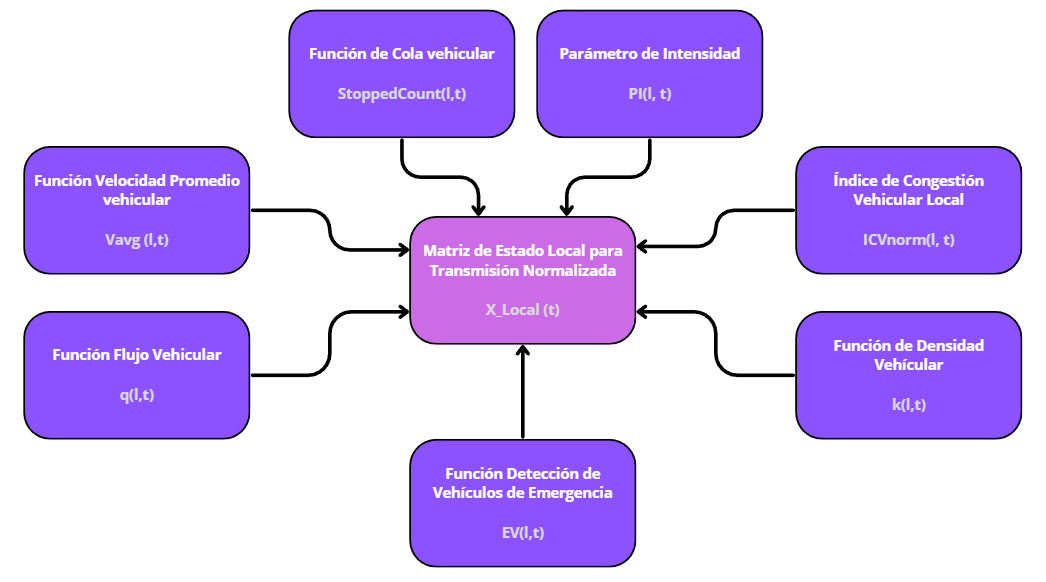
\includegraphics[width=0.92\linewidth,height=0.62\textheight,keepaspectratio]{./media/image143.png}
\captionof*{figure}{\small\itshape Figura 96. Relación de las variables locales con la Matriz de estado Local}
\addcontentsline{lof}{figure}{Figura 96. Relación de las variables locales con la Matriz de estado Local}
\label{fig:96}
\end{center}

\subsection{Transmisión a la Nube}\label{transmisiuxf3n-a-la-nube}

El controlador Raspberry Pi 5 transmite periódicamente un paquete de telemetría comprimido a la plataforma Azure, mediante el módulo 4G LTE Quectel EG25-G, usando el protocolo MQTT sobre TLS:
\begin{centeredmath}
\text{Paquete}_{p}(t)=
\begin{bmatrix}
ID_{\text{interseccion}}\\
\operatorname{timestamp}(t)\\
X_{\text{local}}^{(p)}(t)\\
\phi_{\text{actual}}^{(p)}(t)\\
T_{\text{restante}}^{(p)}(t)\\
\text{estado}_{\text{conexion}}\\
\text{hash}_{\text{integridad}}
\end{bmatrix}
\end{centeredmath}

Variables del paquete:

\begin{itemize}
\item
  \(ID_{\text{intersección}}\): Identificador único.
\item
  \(timestamp(t)\): Marca temporal UTC en formato ISO 8601.
\item
  \(X_{local}^{(p)}(t)\): Matriz de estado local.
\item
  \(\phi_{actual}^{(p)}(t)\): Fase semafórica actualmente activa (0 = NS, 1 = EO, 2 = transición).
\item
  \(T_{restante}^{(p)}(t)\): Tiempo restante de la fase actual (en segundos).
\item
  \(estado_{\text{conexión}}\): Calidad de señal 4G y latencia estimada.
\item
  \(hash_{\text{integridad}}\): Hash SHA-256 para validación de integridad del paquete.
\end{itemize}

\textbf{Coordinación de vehículos de emergencia:}

Cuando la matriz de estado local contiene \(EV_{d} > 0\) para alguna dirección \(d \in \{N, S, E, O\}\), el paquete de telemetría activa un protocolo de transmisión prioritaria que incluye información adicional sobre el vehículo de emergencia:

\begin{centeredmath}
\text{Paquete}_{EV}(t) = \text{Paquete}_{p}(t) \cup \{\, ev_{state}(v_{EV},t),\ prioridad_{nivel} \,\}
\end{centeredmath}

Donde \(ev_{state}(v_{EV},t)\) es el estado completo del vehículo de emergencia rastreado por ByteTrack y \(prioridad_{nivel}\) representa el nivel de urgencia por tipo de vehículo de emergencia.

El paquete de telemetría incluye el \(ID_{\text{intersección}}\), que identifica el origen de los datos, junto con el \(timestamp(t)\) para mantener la trazabilidad temporal. Además, incorpora la matriz \(X_{local}^{(p)}(t)\) que describe el estado sensorial del tráfico, \(\phi_{\text{actual}}^{(p)}(t)\) la fase actual y \(T_{\text{restante}}^{(p)}(t)\) su tiempo restante para coordinar la sincronización semafórica, mientras que el \(estado_{\text{conexión}}\) asegura la calidad del enlace 4G y el \(hash_{\text{integridad}}\) valida la autenticidad de la información transmitida al verificar que el paquete no haya sido alterado.

\section{Sistema de Procesamiento y Control Global}\label{sistema-de-procesamiento-y-control-global}

El procesamiento y la toma de decisiones se centralizan completamente en la plataforma Microsoft Azure, la cual recibe la telemetría de todas las intersecciones, ejecuta algoritmos de optimización global y genera comandos de control individualizados para cada semáforo de la red vial.

\subsection{Registro de Ubicaciones Geográficas en Azure}\label{registro-de-ubicaciones-geogruxe1ficas-en-azure}

Antes de abordar la agregación de estados de red y el procesamiento en tiempo real es necesario establecer un repositorio persistente de las ubicaciones geográficas de todas las intersecciones en la red vial. Dado que las coordenadas GPS de cada intersección son constantes, sería ineficiente transmitirlas repetidamente en cada paquete de telemetría.

Por esta razón, el sistema implementa un registro estático de ubicaciones almacenado en Azure Cosmos DB (base de datos NoSQL distribuida globalmente), que se inicializa durante la fase de instalación y configuración de cada intersección.

\textbf{Estructura del registro:}

\begin{centeredmath}
Registro_{\text{intersección}} = \{\,(ID_{p},\ lat_{p},\ lon_{p},\ metadata_{p})\ :\ p = 1, 2, \ldots, P\,\}
\end{centeredmath}

Donde:

\begin{itemize}
\item
  \textbf{ID}: Identificador único de la intersección
\item
  \textbf{lat}: Latitud en grados decimales (obtenida del módulo GPS del gabinete)
\item
  \textbf{lon}: Longitud en grados decimales (obtenida del módulo GPS del gabinete)
\item
  \textbf{metadata}: Información adicional (dirección postal, distrito, zona, fecha de instalación)
\end{itemize}

Las coordenadas GPS almacenadas en Azure Cosmos DB se utilizan para:

\begin{enumerate}
\def\labelenumi{\arabic{enumi}.}
\item
  \textbf{Cálculo de la matriz de adyacencia}: Las distancias geodésicas \(d_{ij}\) entre intersecciones se calculan una sola vez usando la fórmula de Haversine sobre las coordenadas almacenadas.
\item
  \textbf{Predicción de rutas de vehículos de emergencia}: Cuando una intersección detecta un vehículo de emergencia, Azure consulta las ubicaciones de intersecciones vecinas para predecir trayectorias probables.
\item
  \textbf{Generación de olas verdes prioritarias}: El sistema calcula rutas óptimas entre intersecciones usando las coordenadas GPS para coordinar señales verdes anticipadas.
\item
  \textbf{Visualización en dashboards}: Los mapas de control en tiempo real consultan las ubicaciones para representar gráficamente el estado de la red.
\end{enumerate}

Una visualización de ejemplo de un paquete de envío a Azure y su registro de intersección se muestra en la figura 97.

\begin{center}
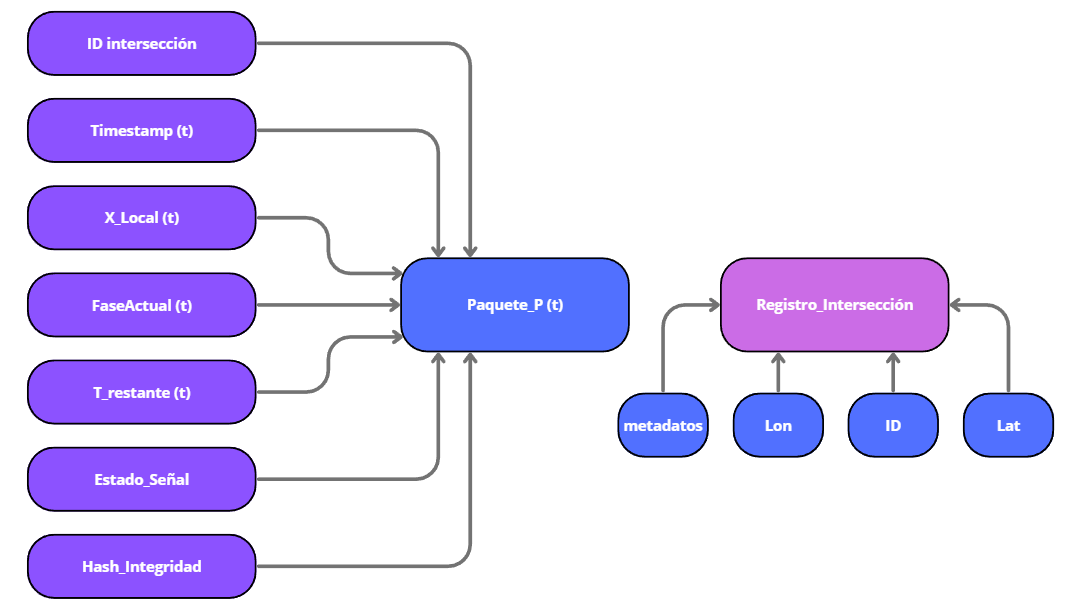
\includegraphics[width=0.92\linewidth,height=0.62\textheight,keepaspectratio]{./media/image50.png}
\captionof*{figure}{\small\itshape Figura 97. Registro y Paquete encontrados en Azure por Intersección.\\}
\addcontentsline{lof}{figure}{Figura 97. Registro y Paquete encontrados en Azure por Intersección.\\}
\label{fig:97}
\end{center}

\subsection{Agregación de Estados de Red y Coordinación de Emergencias}\label{agregaciuxf3n-de-estados-de-red-y-coordinaciuxf3n-de-emergencias}

El estado global del sistema en el instante t se construye mediante la agregación de los estados locales transmitidos por todas las intersecciones P:
\begin{centeredmath}
X_{\text{global}}(t)=
\begin{bmatrix}
X_{\text{local}}^{(1)}(t)\\
X_{\text{local}}^{(2)}(t)\\
\vdots\\
X_{\text{local}}^{(P)}(t)
\end{bmatrix}
\in \mathbb{R}^{P\times 28}
\end{centeredmath}

Esta matriz de alta dimensionalidad, donde P puede variar en cientos de intersecciones en Lima Metropolitana, alimenta simultáneamente tres módulos de procesamiento desplegados en Azure.

\textbf{Sistema de Coordinación de Vehículos de Emergencia:}

El módulo de análisis en tiempo real (Azure Stream Analytics) implementa un subsistema especializado para la detección y seguimiento de vehículos de emergencia a nivel de red. Cuando una intersección \(I_{p}\) detecta un vehículo de emergencia (\(EV_{d}^{(p)} > 0\)), se activa el siguiente protocolo:

\textbf{Extracción de información del vehículo de emergencia:}

\begin{centeredmath}
EV_{event}^{(p)}(t) = \{\, ID_{p},\ DIR_{inicial}(v_{EV}),\ DIR_{salida}(v_{EV}),\ ev_{state}(v_{EV},t),\ timestamp(t) \,\}
\end{centeredmath}

Esta estructura de datos encapsula toda la información relevante sobre la detección de un vehículo de emergencia en la intersección \(I_{p}\) en el instante \(t\). Cada componente tiene un propósito específico en la coordinación de red:

\begin{itemize}
\item
  ID: Identificador único de la intersección donde se detectó el vehículo de emergencia, permitiendo geolocalizar el evento en el grafo vial.
\item
  DIRinicial: Dirección de aproximación del vehículo al entrar al área visible de la cámara (N, S, E, u O), que indica desde qué carril ingresó a la intersección.
\item
  DIRsalida: Dirección de salida proyectada o confirmada del vehículo al abandonar la intersección, crucial para predecir hacia qué intersecciones vecinas se dirige. Esta variable se actualiza continuamente mientras ByteTrack rastrea el vehículo.
\item
  \(ev_{state}\): Estado cinemático completo del vehículo en el instante t.
\item
  timestamp(t): Marca temporal UTC en formato ISO 8601 del evento de detección, esencial para sincronizar acciones coordinadas entre múltiples intersecciones y calcular tiempos estimados de llegada
\end{itemize}

Este paquete de información se transmite inmediatamente a Azure mediante el protocolo MQTT prioritario cuando EVd(p) \textgreater{} 0, activando el subsistema de coordinación de emergencias que procesa estos datos para generar olas verdes anticipadas en intersecciones vecinas.

\textbf{Predicción de trayectoria probable:}

El sistema consulta la base de datos de ubicaciones GPS en Azure Cosmos DB para obtener las coordenadas de la intersección actual (latp, lonp) y de todas las intersecciones vecinas conectadas directamente según la matriz de adyacencia A.

Para cada intersección vecina Ij donde Aij \textgreater{} 0, se calcula:

\begin{itemize}
\item
  Ángulo de aproximación desde Ip hacia Ij usando las coordenadas GPS.
\item
  Compatibilidad direccional comparando DIRsalida(EV) con el ángulo calculado.
\item
  Probabilidad de tránsito basada en patrones históricos de flujo vehicular.
\end{itemize}

Se genera un conjunto de intersecciones candidatas ordenadas por probabilidad:

\begin{centeredmath}
Candidates^{(p)}(t) = \{\,(I_{j},\ prob_{j})\ :\ A_{pj} > 0 \ \land\ compatible\!\left(DIR_{salida}(v_{EV}),\ \angle(I_{p},I_{j})\right)\,\}
\end{centeredmath}

Esta expresión define el conjunto de intersecciones vecinas hacia las cuales el vehículo de emergencia podría dirigirse desde su posición actual. La condición Aij \textgreater{} 0 garantiza que solo se consideren intersecciones con conexión vial directa, mientras que la función\(\ compatible()\) verifica que la dirección de salida observada del vehículo sea geométricamente compatible con el ángulo hacia cada intersección candidata.

La compatibilidad direccional se evalúa calculando la diferencia angular \(\Delta\theta\) entre \(DIR_{salida}\) y el ángulo geográfico \(\angle(I_{p}, I_{j})\). Si \(|\Delta\theta| < \theta_{lim}\) (con \(\theta_{lim} = 45^{\circ}\) como ángulo límite), la intersección se considera candidata. Por ejemplo, si el vehículo sale hacia el Norte y existe una intersección al Noreste, esta será incluida en el conjunto; en cambio, una intersección al Sur sería descartada por incompatibilidad direccional.

Cada par (Ij, probj) en el conjunto incluye la probabilidad probj, calculada integrando la compatibilidad direccional, la distancia dij (intersecciones más cercanas tienen mayor probabilidad) y patrones históricos de flujo vehicular entre Ip e Ij. El conjunto resultante se ordena descendentemente por probabilidad, permitiendo al sistema priorizar las K intersecciones más probables.

\textbf{Generación de ola verde prioritaria:}

Para las K intersecciones con mayor probabilidad, el motor de decisión RL genera comandos de preacondicionamiento:

\begin{centeredmath}
Comando_{EV}^{(j)}(t) = \{\, \phi_{obj} = alinear(DIR_{esp}),\ T_{prev},\ prioridad = \text{ACTIVADA} \,\}
\end{centeredmath}

Donde:

\begin{itemize}
\item
  \(\phi_{obj}:\) representa la fase semafórica objetivo, es decir, la configuración de luces (verde, amarillo, rojo) que debe activarse para permitir el paso libre en la dirección del vehículo de emergencia.
\item
  \(DIR_{esp}:\) es la dirección esperada de desplazamiento del vehículo de emergencia, determinada mediante el análisis de su trayectoria actual y la topología de la red (por ejemplo, norte--sur, este--oeste, o giro).
\item
  \(T_{prev}:\) corresponde al tiempo de anticipación, calculado como:
\end{itemize}

\begin{centeredmath}
T_{prev} = \frac{d_{veh}}{v_{veh}}
\end{centeredmath}

donde \(d_{veh}\) es la distancia entre el vehículo y la intersección, y \(v_{veh}\)\hspace{0pt} es su velocidad actual. Este valor estima cuánto falta para que el vehículo llegue al cruce, lo que permite activar la fase verde con antelación óptima.

\begin{itemize}
\item
  Prioridad = ACTIVA: es una bandera lógica que anula la programación normal del semáforo, priorizando la fase que favorece el paso del vehículo de emergencia.
\end{itemize}

En resumen, el cálculo combina predicción de dirección y tiempo estimado de arribo para determinar cuándo y en qué sentido debe abrirse la ``ola verde''. El motor RL ajusta estos valores dinámicamente según los datos recibidos en tiempo real (posición, velocidad y dirección del vehículo).

Una imagen representativa se ve en la Figura 98.

\begin{center}
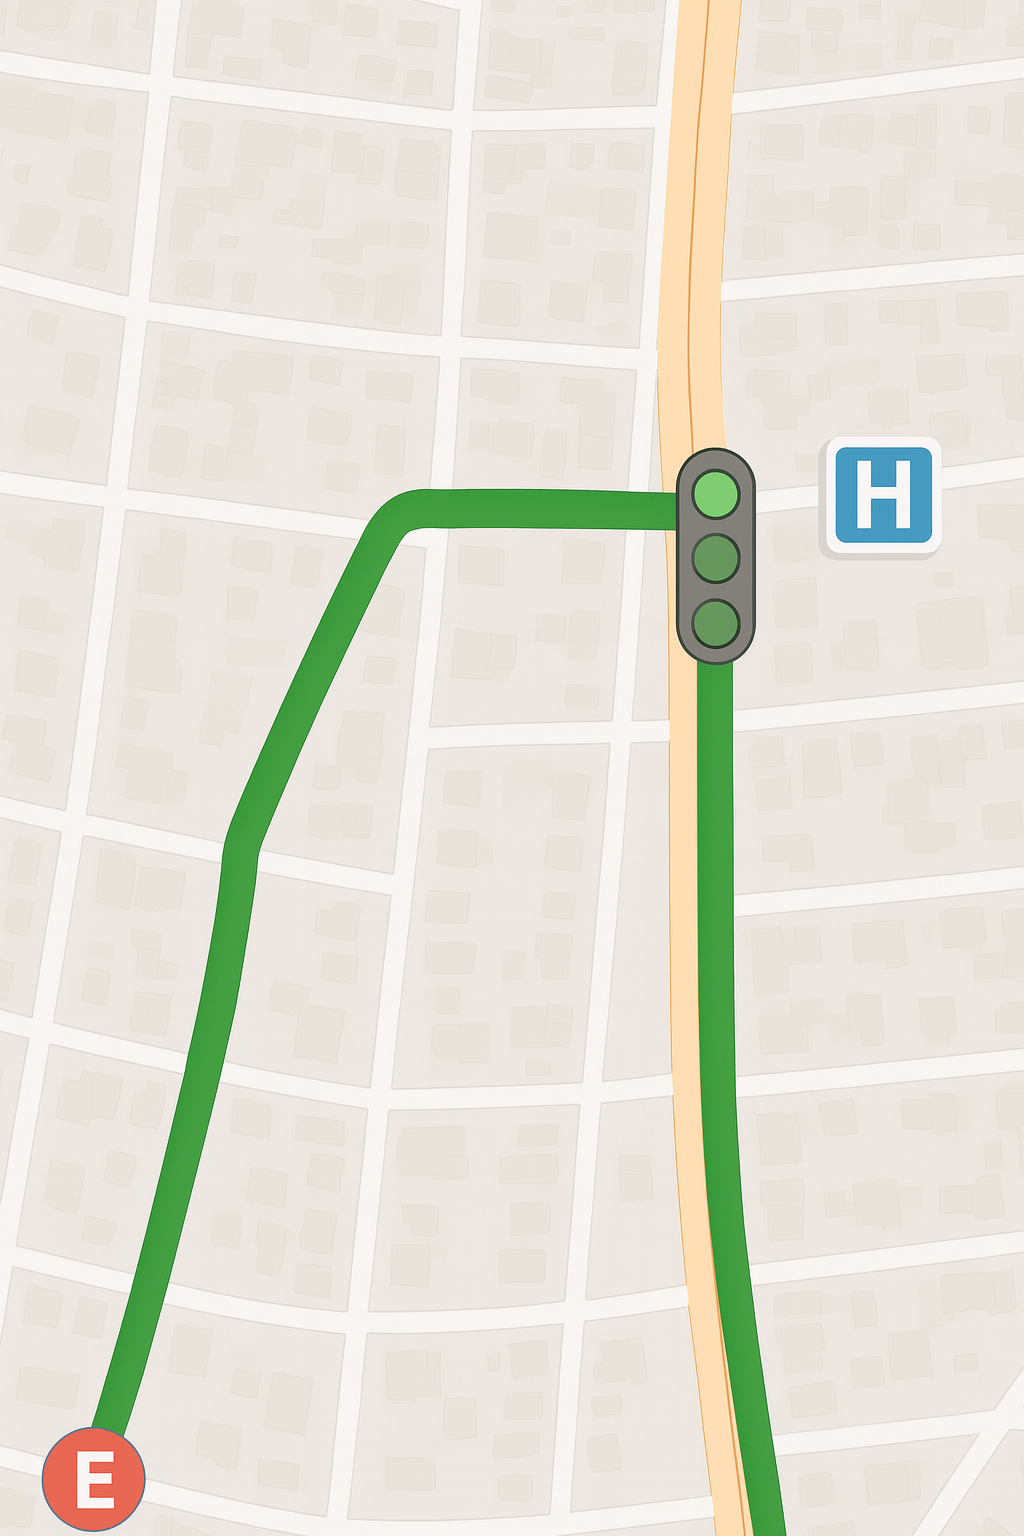
\includegraphics[width=0.92\linewidth,height=0.62\textheight,keepaspectratio]{./media/image112.png}
\captionof*{figure}{\small\itshape Figura 98. Coordinación de ola verde prioritaria para un vehículo de emergencia.}
\addcontentsline{lof}{figure}{Figura 98. Coordinación de ola verde prioritaria para un vehículo de emergencia.}
\label{fig:98}
\end{center}

\textbf{Actualización continua:}

Mientras el vehículo de emergencia permanece en la red (detectado por alguna intersección), el sistema:

\begin{itemize}
\item
  Refina las predicciones de trayectoria con cada nueva detección
\item
  Ajusta las fases semafóricas de intersecciones adelante en la ruta predicha
\item
  Restaura el control normal en intersecciones que el vehículo ya atravesó
\end{itemize}

\textbf{Módulos de procesamiento principales:}

Esta matriz alimenta simultáneamente tres módulos de procesamiento desplegados en Azure:

\textbf{1. Análisis en Tiempo Real (Azure Stream Analytics)}

Este módulo constituye la primera línea de procesamiento de datos telemétricos. Su función principal es la transformación, filtrado y agregación de flujos de datos continuos provenientes de las P intersecciones activas en la red, incluyendo la coordinación especializada de vehículos de emergencia descrita anteriormente.

\textbf{2. Motor de Decisión RL (Azure Machine Learning con GPU)}

En el diseño propuesto, esta capa puede evaluar el estado global mediante una política entrenada \ensuremath{\pi}*, generar recomendaciones de ajuste para cada intersección y predecir la evolución futura del tráfico mediante arquitecturas CNN-LSTM. Este módulo integra las señales de priorización de emergencias con la optimización general de tráfico, manteniendo la validación local antes de cualquier aplicación operativa.

\textbf{3. Análisis Histórico (Azure Synapse Analytics con Apache Spark)}

Este módulo opera en la escala temporal más larga, procesando semanas de datos históricos para extraer patrones, entrenar modelos y formular estrategias de optimización a largo plazo.

Tareas principales:

\begin{itemize}
\item
  Análisis de Patrones Temporales Recurrentes
\item
  Entrenamiento Continuo de Modelos Predictivos
\item
  Calibración de Parámetros del Sistema
\item
  Identificación de Intersecciones Críticas
\item
  Generación de Reportes Ejecutivos
\end{itemize}

\subsection{Matriz de Desempeño de Red}\label{matriz-de-desempeuxf1o-de-red}

Para modelar la topología vial y las relaciones de influencia entre intersecciones, se define una matriz de adyacencia ponderada que representa la estructura física de la red vial y cuantifica la intensidad de interacción entre intersecciones conectadas.

\textbf{Definición de la matriz de adyacencia:}

\begin{centeredmath}
A \in \mathbb{R}^{P \times P}, \qquad
A_{ij} =
\begin{cases}
w_{ij} \cdot d_{ij}^{-\alpha}, & \text{si existe conexión directa entre } I_{i} \text{ e } I_{j}\\[2pt]
0, & \text{caso contrario}
\end{cases}
\end{centeredmath}

Donde:

\(d_{ij}\): distancia geodésica entre intersecciones (en metros), calculada mediante la fórmula de Haversine sobre las coordenadas GPS \((lat, lon)\), expresadas en radianes, almacenadas en Azure Cosmos DB:

\begin{centeredmath}
d_{ij} = 2R \cdot \arcsin\!\left( \sqrt{\, \sin^{2}\!\left(\frac{lat_{j} - lat_{i}}{2}\right) + \cos(lat_{i})\cos(lat_{j})\sin^{2}\!\left(\frac{lon_{j} - lon_{i}}{2}\right) \,} \right)
\end{centeredmath}

Donde \(R \approx 6371\) km representa el radio medio de la Tierra. Para las distancias urbanas de interés (\(d_{ij} < 2\) km), esta fórmula es numéricamente estable y su error respecto a la distancia real sobre el elipsoide es despreciable (\(< 0.5\%\)).

\(w_{ij}\): peso asociado al flujo vehicular promedio histórico entre las intersecciones \(i\) y \(j\), normalizado al rango \([0,1]\).

\(\alpha\): exponente de decaimiento de distancia, que controla cómo disminuye la influencia con la distancia (se adopta \(\alpha = 1\); valores mayores acentúan la localidad de la propagación).

La matriz de adyacencia A captura dos aspectos fundamentales de la conectividad vial:

\begin{itemize}
\item
  \textbf{Proximidad espacial} (\(d_{ij}^{- \alpha}\)): Intersecciones más cercanas tienen mayor influencia mutua, ya que los vehículos transitan más rápidamente entre ellas, propagando congestión con menor demora temporal.
\item
  \textbf{Intensidad de flujo} (\(w_{ij}\)): Vías con mayor volumen vehicular histórico tienen mayor peso, reflejando rutas principales donde la propagación de congestión tiene impacto más significativo.
\end{itemize}

La combinación multiplicativa equilibra ambos factores: una intersección cercana con bajo flujo puede tener influencia similar a una intersección lejana con alto flujo.

\textbf{Criterio de conexión directa:}

Dos intersecciones se consideran directamente conectadas si:

\begin{centeredmath}
A_{ij} > 0 \iff \exists\ \text{vía directa sin intersecciones intermedias entre } I_{i} \text{ e } I_{j}
\end{centeredmath}

Este criterio se verifica mediante mapas digitales de la red vial, identificando segmentos viales que conectan pares de intersecciones sin nodos intermedios.

\textbf{Matriz de grado:}

La matriz D es una matriz diagonal donde cada elemento Dii\hspace{0pt} representa la suma de todas las conexiones que tiene la intersección i:

\begin{centeredmath}
D_{ii} = \sum_{j = 1}^{P}A_{ij}
\end{centeredmath}

Físicamente, Dii cuantifica el ``grado de conectividad ponderado'' de la intersección i: valores altos indican intersecciones altamente conectadas que actúan como hubs en la red vial.

\textbf{Normalización para Graph Neural Networks:}

Para estabilizar el procesamiento mediante Graph Neural Networks (GNN) y evitar que intersecciones altamente conectadas dominen los cálculos, se aplica la normalización simétrica:

\begin{centeredmath}
A_{norm} = D^{- 1/2}AD^{- 1/2}
\end{centeredmath}

Esta transformación realiza una normalización simétrica que preserva propiedades algebraicas importantes:

\textbf{Preservación de simetría}: Si A es simétrica, Anorm también lo es.

\textbf{Acotamiento de valores propios}: Los valores propios de Anorm están acotados en {[}-1, 1{]}.

\textbf{Equilibrio de influencias}: La multiplicación por \(D^{- 1/2}\) reduce el peso de nodos altamente conectados y amplifica el de nodos poco conectados, logrando que cada intersección tenga influencia comparable independientemente de su grado.

La matriz Anorm permite, por tanto la modelación de propagación espacial de congestión, pues captura cómo los embotellamientos en una intersección se propagan a intersecciones vecinas mediante la ecuación de difusión:

\begin{centeredmath}
ICV^{(t + 1)} = \sigma\!\left(A_{norm} \cdot ICV^{(t)} + b\right)
\end{centeredmath}

Donde \(\sigma(\cdot)\) es una función de activación no lineal y \(b \in \mathbb{R}^{P}\) un vector de sesgo (bias).

También el sistema permite identificar intersecciones críticas mediante el análisis de centralidad de intermediación aplicado al grafo A, optimizar la coordinación semafórica utilizando el motor de decisión de refuerzo que emplea Anorm para propagar información entre intersecciones vecinas, y generar olas verdes calculando secuencias de fases verdes coordinadas mediante la resolución de problemas de optimización sobre el grafo ponderado A, con el fin de minimizar los tiempos de parada acumulados en las rutas principales.

La construcción es matemáticamente correcta siempre que:

\begin{enumerate}
\def\labelenumi{\arabic{enumi}.}
\item
  \textbf{A es simétrica}: Aij = Aji (la influencia de i sobre j es igual a la de j sobre i)
\item
  \textbf{D es invertible}: Dii \textgreater{} 0 para todo i (toda intersección tiene al menos una conexión)
\item
  \textbf{A no tiene auto-lazos}: Aii = 0 (una intersección no se influye directamente a sí misma)
\end{enumerate}

En primer lugar, la simetría de la matriz de adyacencia asegura que la influencia entre dos intersecciones sea recíproca, es decir, que si la intersección Ii\hspace{0pt} ejerce algún efecto sobre Ij\hspace{0pt} (por ejemplo, en la propagación de congestión o tiempos de espera), entonces Ij\hspace{0pt} también pueda influir en Ii\hspace{0pt} con la misma intensidad. Esta propiedad refleja la bidireccionalidad inherente de la mayoría de las conexiones viales urbanas, donde el tránsito fluye en ambos sentidos y los fenómenos de congestión o liberación de flujo se retroalimentan espacialmente.

Desde el punto de vista matemático, la simetría también garantiza que la matriz normalizada Anorm conserve propiedades algebraicas como la realidad y acotación de los valores propios, permitiendo aplicar técnicas de análisis espectral, filtrado o aprendizaje sobre grafos sin introducir inestabilidades numéricas. Si la matriz A no fuera simétrica, la propagación modelada perdería coherencia física (pues algunas intersecciones afectarían a otras sin recibir influencia de retorno) y el modelo dejaría de representar una difusión balanceada dentro del sistema.

En segundo lugar, la invertibilidad de la matriz de grado implica que toda intersección debe poseer al menos una conexión directa con otra. En términos físicos, esto significa que ninguna intersección puede considerarse completamente aislada dentro de la red, ya que un nodo sin conexiones no participa en la transmisión de información, tráfico ni congestión. Desde el punto de vista computacional, esta condición es indispensable porque el proceso de normalización \(D^{- 1/2}\) requiere que cada elemento diagonal de D sea distinto de cero; de lo contrario, aparecerían divisiones indefinidas y el sistema perdería significado matemático.

Además, la existencia de al menos una conexión asegura que la intersección pueda ser afectada y afectar a su entorno vial, lo cual es útil para mantener la continuidad topológica de la red. En otras palabras, esta condición garantiza que el modelo describa una red efectivamente conectada y no un conjunto de puntos independientes sin interacción mutua.

Finalmente, la ausencia de auto-lazos se justifica porque una intersección no puede ejercer influencia sobre sí misma en términos de propagación espacial. La variable de desempeño que se calcula (por ejemplo, el índice de congestión vial ICV) ya refleja el estado local de la intersección, por lo que agregar un término de autoinfluencia introduciría una redundancia artificial y alteraría la dinámica del modelo. Desde una perspectiva de grafos, los auto-lazos distorsionan el grado efectivo de los nodos al incrementar sus pesos diagonales, lo que conduce a una sobreponderación del estado local frente a las influencias externas. En consecuencia, el sistema perdería la capacidad de representar correctamente cómo los cambios en una intersección repercuten en sus vecinas, que es precisamente el fenómeno que se busca capturar mediante la ecuación de difusión.

\subsection{Métricas de Desempeño de Red}\label{muxe9tricas-de-desempeuxf1o-de-red}

Las métricas de desempeño de red son indicadores agregados que cuantifican el comportamiento global del sistema semafórico desde una perspectiva de red completa, en contraste con las métricas locales que caracterizan intersecciones individuales. Estas métricas permiten evaluar la efectividad de estrategias de control coordinado y detectar degradaciones sistémicas que no serían evidentes observando intersecciones aisladamente.

\textbf{Consideraciones fundamentales sobre tracking multi-intersección:}

El seguimiento de vehículos individuales a través de múltiples intersecciones presenta desafíos técnicos significativos que hacen impráctica la medición directa de tiempos de viaje puerta a puerta:

\textbf{Problema de reidentificación}: Cada intersección opera con su propia cámara y sistema YOLO independiente. No existe un identificador único global que permita asociar el ``vehículo \#47 detectado en la intersección A'' con el ``vehículo \#23 detectado en la intersección B'' minutos después.

\textbf{Variabilidad de apariencia}: La apariencia visual del mismo vehículo cambia drásticamente entre cámaras debido a diferencias en iluminación, ángulo, distancia y oclusiones, dificultando la reidentificación mediante descriptores visuales

Por estas razones, las métricas propuestas se diseñan para ser estadísticamente representativas del desempeño de red sin requerir tracking individual exhaustivo, utilizando únicamente:

\begin{enumerate}
\def\labelenumi{\arabic{enumi}.}
\item
  \textbf{Variables transmitidas en} Xlocal
\item
  \textbf{Parámetros de configuración almacenados en Azure Cosmos DB} durante la instalación
\end{enumerate}

\textbf{Parámetros de Configuración en Azure Cosmos DB}

Durante la fase de instalación de cada intersección, se registra en Azure Cosmos DB:

\begin{centeredmath}
IConfig_{p} = \{\, ID_{p},\ lat_{p},\ lon_{p},\ [\, C_{max,N}^{(p)},\ C_{max,S}^{(p)},\ C_{max,E}^{(p)},\ C_{max,O}^{(p)} \,] \,\}
\end{centeredmath}

Donde cada \(C_{max,d}^{(p)}\) representa el número máximo de vehículos que pueden ser observados detenidos en el área visible de la cámara en la dirección \(d\).

\subsubsection{Índice de Saturación de Colas de Red}

Cuantifica el nivel de saturación promedio de las colas en toda la red, normalizado por la capacidad observable de cada carril.

\begin{centeredmath}
QL_{red\text{-}ideal}(t) = \frac{1}{4P}\sum_{p = 1}^{P}\ \sum_{d \in \{N, S, E, O\}}\frac{SC_{d}^{(p)}(t)}{C_{max,d}^{(p)}}
\end{centeredmath}

Donde \(SC_{d}^{(p)}(t)\) representa el conteo de vehículos detenidos en dirección \(d\), intersección \(p\).

Dado que \(CamMask\) alterna, en cada instante solo dos direcciones tienen valores observados. Azure implementa una ventana temporal deslizante para obtener la estimación completa:

\begin{centeredmath}
QL_{red}(t) = \frac{1}{4P}\sum_{p = 1}^{P}\ \sum_{d \in \{N, S, E, O\}}\frac{NoNulo\!\left(SC_{d}^{(p)}(t)\right)}{C_{max,d}^{(p)}}
\end{centeredmath}

La función de imputación \(NoNulo(\cdot)\) retiene el último valor observado de cada dirección dentro de la ventana temporal (esquema \emph{last observation carried forward}), con el fin de no operar con valores faltantes. Es importante precisar que la condición de ``observado'' no se infiere del valor numérico --- un carril vacío produce legítimamente \(SC = 0\) --- sino del valor de \(CamMask(I_{p},t)\) que acompaña a cada telemetría: solo las dos direcciones alineadas con la orientación vigente de la cámara se marcan como observadas en ese instante. Puesto que la cámara alterna su orientación con un periodo de pocos segundos, el desfase máximo de la imputación está acotado y no introduce sesgos significativos en las métricas agregadas.

\subsubsection{Velocidad Promedio de Red}

Cuantifica la fluidez promedio del tráfico utilizando la segunda fila de \(X_{local}\):

\begin{centeredmath}
V_{avg,red}(t) = \frac{1}{4P}\sum_{p = 1}^{P}\ \sum_{d \in \{N, S, E, O\}} NoNulo\!\left(V_{avg,d}^{(p)}(t)\right)
\end{centeredmath}

Cabe resaltar que, para su interpretación en unidades físicas, Azure mantiene en Cosmos DB los parámetros \(V_{MAX}\) y \(V_{MIN}\), permitiendo la desnormalización.

\subsubsection{Flujo Promedio de Red}

Cuantifica la tasa de servicio promedio de la red utilizando la tercera fila de \(X_{local}\):

\begin{centeredmath}
q_{red}(t) = \frac{1}{4P}\sum_{p = 1}^{P}\ \sum_{d \in \{N, S, E, O\}} NoNulo\!\left(q_{d}^{(p)}(t)\right)
\end{centeredmath}

Donde \(q_{d}^{(p)}\) es el flujo vehicular normalizado en la dirección \(d\).

\subsubsection{Densidad Promedio de Red}

Cuantifica el nivel promedio de ocupación espacial utilizando la cuarta fila de \(X_{local}\):

\begin{centeredmath}
k_{red}(t) = \frac{1}{4P}\sum_{p = 1}^{P}\ \sum_{d \in \{N, S, E, O\}} NoNulo\!\left(k_{d}^{(p)}(t)\right)
\end{centeredmath}

Donde \(k_{d}^{(p)}\) es la densidad vehicular normalizada.

\subsubsection{Índice de Congestión de Red Ponderado}

Pondera cada intersección según su importancia topológica, utilizando la quinta fila de \(X_{local}\):

\begin{centeredmath}
ICV_{red}(t) = \frac{\displaystyle\sum_{p = 1}^{P} w_{p}\, ICV_{\text{intersección}}^{(p)}(t)}{\displaystyle\sum_{p = 1}^{P} w_{p}}
\end{centeredmath}

Donde:

\begin{centeredmath}
ICV_{\text{intersección}}^{(p)}(t) = \frac{1}{4}\sum_{d \in \{N, S, E, O\}} NoNulo\!\left(ICV_{d}^{(p)}(t)\right)
\end{centeredmath}

\begin{centeredmath}
w_{p} = \frac{BC(p)}{\displaystyle\sum_{j = 1}^{P}BC(j)}
\end{centeredmath}

\begin{itemize}
\item
  \(ICV_{d}^{(p)}\): índice de congestión vehicular normalizado.
\item
  \(BC(p)\): centralidad de intermediación (calculada una vez sobre la matriz A y almacenada en Cosmos DB).
\item
  \(w_{p}:\) peso normalizado, \(\sum_{p} w_{p} = 1\).
\end{itemize}

Cálculo de \(BC(p)\): se realiza fuera de línea durante la configuración inicial usando el algoritmo de Brandes, de complejidad \(O(PE + P^{2}\log P)\) para grafos ponderados con \(E\) aristas, sobre la matriz de adyacencia A. Los valores resultantes se almacenan en Cosmos DB como parte de \(IConfig\).

\subsubsection{Parámetro de Intensidad Promedio de Red}

Cuantifica la eficiencia promedio utilizando la sexta fila de \(X_{local}\):

\begin{centeredmath}
PI_{red}(t) = \frac{1}{4P}\sum_{p = 1}^{P}\ \sum_{d \in \{N, S, E, O\}} NoNulo\!\left(PI_{d}^{(p)}(t)\right)
\end{centeredmath}

Donde \(PI\) es el parámetro de intensidad normalizado: valores cercanos a 1 indican una red semafórica eficiente, y valores cercanos a 0 una red congestionada.

\subsubsection{Variabilidad Temporal de Red}

Azure calcula tendencias temporales sobre las métricas agregadas mediante diferencias finitas:

\begin{centeredmath}
\Delta X_{red}(t) = X_{red}(t) - X_{red}(t - \Delta t)
\end{centeredmath}

Donde \(X \in \{QL,\ V_{avg},\ q,\ k,\ ICV,\ PI\}\). El signo y la magnitud de \(\Delta X_{red}\) permiten distinguir congestión en formación (\(\Delta ICV_{red} > 0\)) de congestión en disipación (\(\Delta ICV_{red} < 0\)), información que se incorpora al estado del módulo de optimización global.

\subsection{Optimización de Olas Verdes}\label{optimizaciuxf3n-de-olas-verdes}

La optimización de olas verdes busca maximizar el throughput vehicular en corredores viales principales, permitiendo que pelotones de vehículos atraviesen múltiples intersecciones consecutivas sin detenerse. Esta coordinación se logra mediante el cálculo de offsets temporales óptimos entre semáforos adyacentes.

Para un corredor vial con \(n\) intersecciones consecutivas \(\{I_1, I_2, \ldots, I_n\}\) separadas por distancias \(\{d_1, d_2, \ldots, d_{n-1}\}\), el offset óptimo \(\tau_{i,i+1}^{*}\) entre intersecciones consecutivas se define como el desfase temporal que minimiza el número esperado de paradas vehiculares:

\begin{centeredmath}
\tau_{i,i+1}^{*} = \operatorname*{arg\,min}_{\tau \in [0,\,T_{\text{ciclo}})} P_{\text{medio}}(\tau)
\end{centeredmath}

Donde \(\tau\) es el desfase temporal entre los inicios de luz verde de dos intersecciones consecutivas y \(P_{\text{medio}}(\tau)\) es el número promedio de paradas que experimentan los vehículos en función del desfase elegido. El offset se restringe al rango \([0, T_{\text{ciclo}})\), siendo \(T_{\text{ciclo}}\) la duración total del ciclo semafórico.

El desfase debe ser tal que, si un vehículo parte de la primera intersección justo cuando el semáforo se pone verde y circula a una velocidad constante \(v_{\text{prog}}\), llegue a la siguiente intersección también cuando esta esté en verde, creando así una ``ola verde''. El offset ideal se calcula como:

\begin{centeredmath}
\tau_{i,i+1} = \frac{d_i}{v_{\text{prog}}} \bmod T_{\text{ciclo}}
\end{centeredmath}

Cabe recordar que \(d_i\) es la distancia entre dos intersecciones calculada con Haversine sobre coordenadas GPS de Cosmos DB, \(v_{\text{prog}}\) la velocidad de progresión y \(T_{\text{ciclo}}\) la duración del ciclo.

Consideremos un vehículo que sale de la intersección \(I_i\) en el instante \(t_0\) cuando inicia el verde. El tiempo que requiere para llegar a la intersección \(I_{i+1}\), distante \(d_i\) metros, es:

\begin{centeredmath}
t_{\text{viaje}} = \frac{d_i}{v_{\text{prog}}}
\end{centeredmath}

Para que encuentre luz verde al llegar, el semáforo de \(I_{i+1}\) debe iniciar su fase verde en:

\begin{centeredmath}
t_{\text{verde}}^{i+1} = t_0 + t_{\text{viaje}} + kT_{\text{ciclo}}
\end{centeredmath}

Donde \(k\) pertenece a los números enteros y es el número de ciclos transcurridos. Dado que trabajamos con offsets dentro de un ciclo, aplicamos la operación módulo:

\begin{centeredmath}
\tau_{i,i+1} = t_{\text{viaje}} \bmod T_{\text{ciclo}} = \frac{d_i}{v_{\text{prog}}} \bmod T_{\text{ciclo}}
\end{centeredmath}

\subsubsection{Velocidad de Progresión Adaptativa}

La velocidad de progresión \(v_{\text{prog}}\) se calcula dinámicamente utilizando las velocidades transmitidas en \(X_{\text{local}}\) (desnormalizadas mediante \(V_{MAX}\)):

\begin{centeredmath}
v_{\text{prog}} = \min\left(v_{\text{limite}},\ \frac{1}{n}\sum_{i=1}^{n}V_{\text{avg,corredor}}^{(i)}(t)\cdot V_{MAX}\right)
\end{centeredmath}

Donde \(v_{\text{limite}}\) es la velocidad máxima legal del corredor, almacenada en Cosmos DB. El operador \(\min\) garantiza que la ola verde nunca se programe para una velocidad superior a la permitida, evitando incentivar excesos de velocidad.

\subsubsection{Ancho de Banda Verde}

El ancho de banda verde mide la fracción del ciclo durante la cual existe una ventana continua de progresión en verde a lo largo de todo el corredor:

\begin{centeredmath}
BW_{\text{verde}} = \min_{i=1,\ldots,n-1}\left[\frac{T_{\text{verde},i}-\left|\,\tau_{i,i+1}-t_{\text{viaje},i} \bmod T_{\text{ciclo}}\,\right|}{T_{\text{ciclo}}}\right]
\end{centeredmath}

donde \(T_{\text{verde},i}\) es determinado por el módulo de recomendación y el operador \(\min\) identifica el cuello de botella temporal del corredor: la intersección cuyo desajuste entre el offset implementado y el tiempo de viaje real más reduce la ventana de progresión.

\subsubsection{Implementación en Azure}

El módulo de optimización de olas verdes opera en Azure Stream Analytics mediante el siguiente procedimiento:

\begin{enumerate}
\def\labelenumi{\arabic{enumi}.}
\item
  El sistema analiza la matriz de adyacencia A para identificar secuencias de intersecciones conectadas linealmente que forman corredores principales.
\item
  Para cada par consecutivo en el corredor, se consultan las coordenadas GPS de Cosmos DB y se calcula \(d_i\) mediante la fórmula de Haversine.
\item
  Se agregan las velocidades promedio V\_avg de todas las intersecciones del corredor para calcular v\_prog.
\item
  Se aplica la fórmula \(\tau_{i,i + 1}\ \)para cada par consecutivo.
\item
  Se calcula BW\_verde para verificar que la configuración propuesta sea viable. Si BW\_verde \textless{} 0.3, el sistema incrementa progresivamente los tiempos verdes T\_verde,i hasta alcanzar un ancho de banda aceptable. Este incremento está acotado por las restricciones de seguridad del ciclo: extender el verde del corredor consume tiempo de las fases transversales, por lo que el algoritmo nunca sacrifica el mínimo peatonal ni excede \(T_{\text{verde,max}}\) --- la práctica de coordinación advierte que ciclos excesivamente largos trasladan la congestión a las vías laterales aunque aumenten la capacidad teórica del corredor.
\item
  Los offsets calculados se convierten en parámetros sugeridos que la central semafórica valida antes de cualquier aplicación operativa.
\end{enumerate}

\subsection{Sistema de Control Difuso Local}\label{sistema-de-control-difuso-local}

Antes de transmitir datos a Azure, cada intersección implementa un controlador difuso local que genera ajustes inmediatos de fase basados en las condiciones actuales del tráfico. Este subsistema opera con latencia baja y proporciona respuesta reactiva mientras el motor RL en Azure calcula optimizaciones globales.

\subsubsection{Variables Lingüísticas de Entrada}

El sistema difuso procesa tres variables principales derivadas de la matriz de estado local. Todas las funciones de pertenencia son trapezoidales o triangulares, elegidas por su bajo costo computacional en el Raspberry Pi 5 (evaluación en tiempo \(O(1)\) por conjunto) y por su interpretabilidad directa para los operadores de tránsito. Los puntos de quiebre se calibraron a partir de los percentiles de la distribución histórica de cada variable en la simulación, y los conjuntos adyacentes se traslapan para asegurar transiciones de control suaves: para todo valor de entrada, al menos un conjunto tiene pertenencia no nula.

\textbf{Variable 1: Índice de Congestión Vehicular (ICV)}

Para cada dirección d \ensuremath{\in} \{N, S, E, O\}, el ICV normalizado se mapea a tres conjuntos difusos mediante funciones de pertenencia trapezoidales y triangulares:
\begin{centeredmath}
\begin{aligned}
\mu_{\text{Bajo}}(ICV)
&=
\begin{cases}
1, & \text{si } ICV \le 0.2\\
\dfrac{0.4-ICV}{0.2}, & \text{si } 0.2 < ICV \le 0.4\\
0, & \text{si } ICV > 0.4
\end{cases}\\[1em]
\mu_{\text{Medio}}(ICV)
&=
\begin{cases}
0, & \text{si } ICV \le 0.2\\
\dfrac{ICV-0.2}{0.2}, & \text{si } 0.2 < ICV \le 0.4\\
\dfrac{0.7-ICV}{0.3}, & \text{si } 0.4 < ICV \le 0.7\\
0, & \text{si } ICV > 0.7
\end{cases}\\[1em]
\mu_{\text{Alto}}(ICV)
&=
\begin{cases}
0, & \text{si } ICV \le 0.4\\
\dfrac{ICV-0.4}{0.3}, & \text{si } 0.4 < ICV \le 0.7\\
1, & \text{si } ICV > 0.7
\end{cases}
\end{aligned}
\end{centeredmath}

Obsérvese que en todo el dominio se cumple \(\mu_{\text{Bajo}} + \mu_{\text{Medio}} + \mu_{\text{Alto}} = 1\) (partición difusa de Ruspini), lo que garantiza que la suma de activaciones esté normalizada y simplifica el análisis de estabilidad del controlador.

\textbf{Variable 2: Parámetro de Intensidad (PI)}

Indica eficiencia del flujo vehicular:
\begin{centeredmath}
\begin{aligned}
\mu_{\text{Ineficiente}}(PI)
&=
\begin{cases}
1, & \text{si } PI \le 0.3\\
\dfrac{0.5-PI}{0.2}, & \text{si } 0.3 < PI \le 0.5\\
0, & \text{si } PI > 0.5
\end{cases}\\[1em]
\mu_{\text{Moderadamente\_Eficiente}}(PI)
&=
\begin{cases}
0, & \text{si } PI \le 0.3\\
\dfrac{PI-0.3}{0.2}, & \text{si } 0.3 < PI \le 0.5\\
\dfrac{0.8-PI}{0.3}, & \text{si } 0.5 < PI \le 0.8\\
0, & \text{si } PI > 0.8
\end{cases}\\[1em]
\mu_{\text{Muy\_Eficiente}}(PI)
&=
\begin{cases}
0, & \text{si } PI \le 0.5\\
\dfrac{PI-0.5}{0.3}, & \text{si } 0.5 < PI \le 0.8\\
1, & \text{si } PI > 0.8
\end{cases}
\end{aligned}
\end{centeredmath}

\textbf{Variable 3: Presencia de Vehículos de Emergencia (EV)}

Al tratarse de un conteo entero, esta variable se modela mediante conjuntos nítidos (singleton), un caso límite válido de conjunto difuso:
\begin{centeredmath}
\begin{aligned}
\mu_{\text{Ausente}}(EV)
&=
\begin{cases}
1, & \text{si } EV=0\\
0, & \text{si } EV>0
\end{cases}\\[1em]
\mu_{\text{Presente}}(EV)
&=
\begin{cases}
0, & \text{si } EV=0\\
1, & \text{si } EV>0
\end{cases}
\end{aligned}
\end{centeredmath}

\subsubsection{Variable Lingüística de Salida}

\textbf{Ajuste de Tiempo Verde (\ensuremath{\Delta}Tverde)}

Modificación porcentual del tiempo de fase verde respecto al ciclo base, definida sobre el universo de discurso \(\Delta T \in [-30\%,\ +30\%]\) mediante cinco conjuntos difusos:
\begin{centeredmath}
\begin{aligned}
\mu_{\text{Reducir\_Fuerte}}(\Delta T)
&=
\begin{cases}
1, & \text{si } \Delta T \le -30\%\\
\dfrac{-10\%-\Delta T}{20\%}, & \text{si } -30\% < \Delta T \le -10\%\\
0, & \text{si } \Delta T > -10\%
\end{cases}\\[1em]
\mu_{\text{Reducir\_Leve}}(\Delta T)
&=
\begin{cases}
0, & \text{si } \Delta T \le -30\%\\
\dfrac{\Delta T+30\%}{20\%}, & \text{si } -30\% < \Delta T \le -10\%\\
\dfrac{-5\%-\Delta T}{5\%}, & \text{si } -10\% < \Delta T \le -5\%\\
0, & \text{si } \Delta T > -5\%
\end{cases}
\end{aligned}
\end{centeredmath}

\begin{centeredmath}
\begin{aligned}
\mu_{\text{Mantener}}(\Delta T)
&=
\begin{cases}
0, & \text{si } \Delta T \le -10\%\\
\dfrac{\Delta T+10\%}{10\%}, & \text{si } -10\% < \Delta T \le 0\%\\
\dfrac{10\%-\Delta T}{10\%}, & \text{si } 0\% < \Delta T \le 10\%\\
0, & \text{si } \Delta T > 10\%
\end{cases}\\[1em]
\mu_{\text{Extender\_Leve}}(\Delta T)
&=
\begin{cases}
0, & \text{si } \Delta T \le 5\%\\
\dfrac{\Delta T-5\%}{10\%}, & \text{si } 5\% < \Delta T \le 15\%\\
\dfrac{30\%-\Delta T}{15\%}, & \text{si } 15\% < \Delta T \le 30\%\\
0, & \text{si } \Delta T > 30\%
\end{cases}\\[1em]
\mu_{\text{Extender\_Fuerte}}(\Delta T)
&=
\begin{cases}
0, & \text{si } \Delta T \le 15\%\\
\dfrac{\Delta T-15\%}{15\%}, & \text{si } 15\% < \Delta T \le 30\%\\
1, & \text{si } \Delta T > 30\%
\end{cases}
\end{aligned}
\end{centeredmath}

\subsubsection{Base de Reglas Difusas}

El sistema implementa 12 reglas estructuradas jerárquicamente, organizadas en 4 niveles de prioridad. La base de reglas es \emph{completa}: cuando hay vehículo de emergencia, las 3 reglas de Prioridad 1 cubren los tres niveles de ICV (el PI se ignora deliberadamente, pues la prioridad absoluta del vehículo de emergencia domina cualquier consideración de eficiencia); cuando no lo hay, las 9 reglas restantes cubren exhaustivamente las \(3 \times 3\) combinaciones de ICV y PI. Por lo tanto, para cualquier estado de entrada existe al menos una regla activa y la salida del controlador está siempre definida:

\textbf{Prioridad 1: Reglas de Emergencia (Máxima Prioridad)}

\Needspace{6\baselineskip}
\captionof*{table}{\small\bfseries Tabla 6.1. Reglas de Emergencia (Prioridad 1)}
\addcontentsline{lot}{table}{Tabla 6.1. Reglas de Emergencia (Prioridad 1)}
\label{tbl:6.1}

\begin{longtable}[]{@{}
  >{\raggedright\arraybackslash}p{(\columnwidth - 2\tabcolsep) * \real{0.5000}}
  >{\raggedright\arraybackslash}p{(\columnwidth - 2\tabcolsep) * \real{0.5000}}@{}}
\toprule
\begin{minipage}[b]{\linewidth}\raggedright
\textbf{R1:} SI EV = Presente Y ICV = Alto
\end{minipage} & \begin{minipage}[b]{\linewidth}\raggedright
\textbf{ENTONCES} \ensuremath{\Delta}Tverde = Extender\_Fuerte
\end{minipage} \\
\begin{minipage}[b]{\linewidth}\raggedright
\textbf{R2:} SI EV = Presente Y ICV = Medio
\end{minipage} & \begin{minipage}[b]{\linewidth}\raggedright
\textbf{ENTONCES} \ensuremath{\Delta}Tverde = Extender\_Fuerte
\end{minipage} \\
\begin{minipage}[b]{\linewidth}\raggedright
\textbf{R3:} SI EV = Presente Y ICV = Bajo
\end{minipage} & \begin{minipage}[b]{\linewidth}\raggedright
\textbf{ENTONCES} \ensuremath{\Delta}Tverde = Extender\_Leve
\end{minipage} \\
\midrule
\endhead
\bottomrule
\endlastfoot
\end{longtable}

\textbf{Prioridad 2: Reglas de Congestión Severa}

\Needspace{6\baselineskip}
\captionof*{table}{\small\bfseries Tabla 6.2. Reglas de Congestión Severa (Prioridad 2)}
\addcontentsline{lot}{table}{Tabla 6.2. Reglas de Congestión Severa (Prioridad 2)}
\label{tbl:6.2}

\begin{longtable}[]{@{}
  >{\raggedright\arraybackslash}p{(\columnwidth - 2\tabcolsep) * \real{0.5000}}
  >{\raggedright\arraybackslash}p{(\columnwidth - 2\tabcolsep) * \real{0.5000}}@{}}
\toprule
\begin{minipage}[b]{\linewidth}\raggedright
\textbf{R4:} SI EV = Ausente Y ICV = Alto Y PI = Ineficiente
\end{minipage} & \begin{minipage}[b]{\linewidth}\raggedright
\textbf{ENTONCES} \ensuremath{\Delta}Tverde = Extender\_Fuerte
\end{minipage} \\
\begin{minipage}[b]{\linewidth}\raggedright
\textbf{R5:} SI EV = Ausente Y ICV = Alto Y PI = Moderadamente\_Eficiente
\end{minipage} & \begin{minipage}[b]{\linewidth}\raggedright
\textbf{ENTONCES} \ensuremath{\Delta}Tverde = Extender\_Leve
\end{minipage} \\
\begin{minipage}[b]{\linewidth}\raggedright
\textbf{R6:} SI EV = Ausente Y ICV = Alto Y PI = Muy\_Eficiente
\end{minipage} & \begin{minipage}[b]{\linewidth}\raggedright
\textbf{ENTONCES} \ensuremath{\Delta}Tverde = Mantener
\end{minipage} \\
\midrule
\endhead
\bottomrule
\endlastfoot
\end{longtable}

\textbf{Prioridad 3: Reglas de Congestión Moderada}

\Needspace{6\baselineskip}
\captionof*{table}{\small\bfseries Tabla 6.3. Reglas de Congestión Moderada (Prioridad 3)}
\addcontentsline{lot}{table}{Tabla 6.3. Reglas de Congestión Moderada (Prioridad 3)}
\label{tbl:6.3}

\begin{longtable}[]{@{}
  >{\raggedright\arraybackslash}p{(\columnwidth - 2\tabcolsep) * \real{0.5000}}
  >{\raggedright\arraybackslash}p{(\columnwidth - 2\tabcolsep) * \real{0.5000}}@{}}
\toprule
\begin{minipage}[b]{\linewidth}\raggedright
\textbf{R7:} SI EV = Ausente Y ICV = Medio Y PI = Ineficiente
\end{minipage} & \begin{minipage}[b]{\linewidth}\raggedright
\textbf{ENTONCES} \ensuremath{\Delta}Tverde = Extender\_Leve
\end{minipage} \\
\begin{minipage}[b]{\linewidth}\raggedright
\textbf{R8:} SI EV = Ausente Y ICV = Medio Y PI = Moderadamente\_Eficiente
\end{minipage} & \begin{minipage}[b]{\linewidth}\raggedright
\textbf{ENTONCES} \ensuremath{\Delta}Tverde = Mantener
\end{minipage} \\
\begin{minipage}[b]{\linewidth}\raggedright
\textbf{R9:} SI EV = Ausente Y ICV = Medio Y PI = Muy\_Eficiente
\end{minipage} & \begin{minipage}[b]{\linewidth}\raggedright
\textbf{ENTONCES} \ensuremath{\Delta}Tverde = Reducir\_Leve
\end{minipage} \\
\midrule
\endhead
\bottomrule
\endlastfoot
\end{longtable}

\textbf{Prioridad 4: Reglas de Flujo Libre}

\Needspace{6\baselineskip}
\captionof*{table}{\small\bfseries Tabla 6.4. Reglas de Flujo Libre (Prioridad 4)}
\addcontentsline{lot}{table}{Tabla 6.4. Reglas de Flujo Libre (Prioridad 4)}
\label{tbl:6.4}

\begin{longtable}[]{@{}
  >{\raggedright\arraybackslash}p{(\columnwidth - 2\tabcolsep) * \real{0.5000}}
  >{\raggedright\arraybackslash}p{(\columnwidth - 2\tabcolsep) * \real{0.5000}}@{}}
\toprule
\begin{minipage}[b]{\linewidth}\raggedright
\textbf{R10:} SI EV = Ausente Y ICV = Bajo Y PI = Ineficiente
\end{minipage} & \begin{minipage}[b]{\linewidth}\raggedright
\textbf{ENTONCES} \ensuremath{\Delta}Tverde = Mantener
\end{minipage} \\
\begin{minipage}[b]{\linewidth}\raggedright
\textbf{R11:} SI EV = Ausente Y ICV = Bajo Y PI = Moderadamente\_Eficiente
\end{minipage} & \begin{minipage}[b]{\linewidth}\raggedright
\textbf{ENTONCES} \ensuremath{\Delta}Tverde = Reducir\_Leve
\end{minipage} \\
\begin{minipage}[b]{\linewidth}\raggedright
\textbf{R12:} SI EV = Ausente Y ICV = Bajo Y PI = Muy\_Eficiente
\end{minipage} & \begin{minipage}[b]{\linewidth}\raggedright
\textbf{ENTONCES} \ensuremath{\Delta}Tverde = Reducir\_Fuerte
\end{minipage} \\
\midrule
\endhead
\bottomrule
\endlastfoot
\end{longtable}

\subsubsection{Mecanismo de Inferencia Difusa}

El sistema utiliza el método de Mamdani con cuatro etapas secuenciales:

\textbf{Etapa 1: Fuzzificación}

Para cada dirección d, se calculan los grados de pertenencia aplicando las funciones de pertenencia definidas previamente:
\begin{centeredmath}
\begin{aligned}
\alpha_{ICV_d} &= \left[
\mu_{\text{Bajo}}(ICV_d),\,
\mu_{\text{Medio}}(ICV_d),\,
\mu_{\text{Alto}}(ICV_d)
\right]\\[0.8em]
\alpha_{PI_d} &= \left[
\mu_{\text{Inef}}(PI_d),\,
\mu_{\text{ModEf}}(PI_d),\,
\mu_{\text{MuyEf}}(PI_d)
\right]\\[0.8em]
\alpha_{EV_d} &= \left[
\mu_{\text{Ausente}}(EV_d),\,
\mu_{\text{Presente}}(EV_d)
\right]
\end{aligned}
\end{centeredmath}

\textbf{Etapa 2: Aplicación de Reglas (Operador MIN)}

Para cada regla R\ensuremath{_{i}} con antecedente compuesto (conjunción ``Y''), se calcula el grado de activación mediante la t-norma del mínimo:
\begin{centeredmath}
\alpha_i=
\min\left(
\mu_{\text{antecedente},1},\,
\mu_{\text{antecedente},2},\,
\ldots,\,
\mu_{\text{antecedente},n}
\right)
\end{centeredmath}

\textbf{Etapa 3: Agregación de Consecuentes (Operador MAX)}

Los consecuentes activados, escalados por el grado de activación \(\alpha_{i}\) de su regla (implicación de Mamdani), se agregan mediante la s-norma del máximo para formar la función de pertenencia resultante:
\begin{centeredmath}
\mu_{\text{agregado}}(\Delta T)=
\max\left(
\alpha_1\cdot\mu_{\text{consecuente},1}(\Delta T),\,
\alpha_2\cdot\mu_{\text{consecuente},2}(\Delta T),\,
\ldots
\right)
\end{centeredmath}

\textbf{Etapa 4: Defuzzificación (Método del Centroide)}

Se calcula el valor nítido de salida mediante el centroide de la función agregada:
\begin{centeredmath}
\Delta T_{\text{verde}}^{*}=
\frac{
\int \Delta T\cdot \mu_{\text{agregado}}(\Delta T)\,d\Delta T
}{
\int \mu_{\text{agregado}}(\Delta T)\,d\Delta T
}
\end{centeredmath}

En implementación discreta (ejecutada en el Raspberry Pi 5), el universo \([-30\%, +30\%]\) se discretiza en \(M = 61\) puntos con paso de \(1\%\), y el centroide se aproxima por la suma ponderada:
\begin{centeredmath}
\Delta T_{\text{verde}}^{*}=
\frac{
\sum_{i=1}^{M} \left(\Delta T_i\cdot\mu_{\text{agregado}}(\Delta T_i)\right)
}{
\sum_{i=1}^{M} \mu_{\text{agregado}}(\Delta T_i)
}
\end{centeredmath}

El método del centroide se prefiere sobre alternativas como el máximo de pertenencia (MOM) porque produce una superficie de control continua: pequeñas variaciones del ICV o del PI generan pequeñas variaciones de \(\Delta T_{\text{verde}}^{*}\), evitando saltos abruptos en los tiempos de fase que inducirían oscilaciones en el tráfico.

Una síntesis de lo comentado se encuentra en la siguiente Tabla 6.5.

\Needspace{6\baselineskip}
\captionof*{table}{\small\bfseries Tabla 6.5. Organización Lógica Difusa}
\addcontentsline{lot}{table}{Tabla 6.5. Organización Lógica Difusa}
\label{tbl:6.5}

\begin{longtable}[]{@{}
  >{\raggedright\arraybackslash}p{(\columnwidth - 6\tabcolsep) * \real{0.2070}}
  >{\raggedright\arraybackslash}p{(\columnwidth - 6\tabcolsep) * \real{0.2252}}
  >{\raggedright\arraybackslash}p{(\columnwidth - 6\tabcolsep) * \real{0.3361}}
  >{\raggedright\arraybackslash}p{(\columnwidth - 6\tabcolsep) * \real{0.2318}}@{}}
\toprule
\begin{minipage}[b]{\linewidth}\raggedright
\textbf{Etapa}
\end{minipage} & \begin{minipage}[b]{\linewidth}\raggedright
\textbf{Operador/Método}
\end{minipage} & \begin{minipage}[b]{\linewidth}\raggedright
\textbf{Proceso}
\end{minipage} & \begin{minipage}[b]{\linewidth}\raggedright
\textbf{Salida}
\end{minipage} \\
\begin{minipage}[b]{\linewidth}\raggedright
\textbf{Fuzzificación}
\end{minipage} & \begin{minipage}[b]{\linewidth}\raggedright
Funciones de pertenencia
\end{minipage} & \begin{minipage}[b]{\linewidth}\raggedright
Calcular grados de pertenencia \ensuremath{\mu} para cada variable de entrada en cada dirección d.
\end{minipage} & \begin{minipage}[b]{\linewidth}\raggedright
Valores difusos: \ensuremath{\mu}\_Bajo, \ensuremath{\mu}\_Medio, \ensuremath{\mu}\_Alto
\end{minipage} \\
\begin{minipage}[b]{\linewidth}\raggedright
\textbf{Aplicación de Reglas}
\end{minipage} & \begin{minipage}[b]{\linewidth}\raggedright
Operador MIN
\end{minipage} & \begin{minipage}[b]{\linewidth}\raggedright
Evaluar reglas difusas calculando el mínimo de los grados de pertenencia de las premisas.
\end{minipage} & \begin{minipage}[b]{\linewidth}\raggedright
Grado de activación \ensuremath{\alpha}\ensuremath{_{i}} para cada regla.
\end{minipage} \\
\begin{minipage}[b]{\linewidth}\raggedright
\textbf{Agregación de Consecuentes}
\end{minipage} & \begin{minipage}[b]{\linewidth}\raggedright
Operador MAX
\end{minipage} & \begin{minipage}[b]{\linewidth}\raggedright
Combinar consecuentes activados mediante operador MAX.
\end{minipage} & \begin{minipage}[b]{\linewidth}\raggedright
Función de pertenencia agregada.
\end{minipage} \\
\begin{minipage}[b]{\linewidth}\raggedright
\textbf{Defuzzificación}
\end{minipage} & \begin{minipage}[b]{\linewidth}\raggedright
Método del Centroide
\end{minipage} & \begin{minipage}[b]{\linewidth}\raggedright
Calcular valor nítido mediante centroide (suma ponderada en implementación discreta).
\end{minipage} & \begin{minipage}[b]{\linewidth}\raggedright
Ajuste porcentual \ensuremath{\Delta}T\ensuremath{^{*}} del tiempo verde.
\end{minipage} \\
\midrule
\endhead
\bottomrule
\endlastfoot
\end{longtable}

\subsubsection{Cálculo del Tiempo de Fase Ajustado}

El tiempo verde definitivo para la dirección d se calcula aplicando el ajuste porcentual:
\begin{centeredmath}
T_{\text{verde},d}(t)=
T_{\text{base},d}\left(1+\frac{\Delta T_{\text{verde},d}^{*}}{100}\right)
\end{centeredmath}

Sujeto a restricciones de seguridad:
\begin{centeredmath}
T_{\text{verde,min}} \le T_{\text{verde},d}(t) \le T_{\text{verde,max}}
\end{centeredmath}

Donde:

\begin{itemize}
\item
  Tverde,min = 10s (mínimo para cruce peatonal seguro)
\item
  Tverde,max = 120s (máximo para evitar acumulación excesiva en dirección perpendicular)
\end{itemize}

Si el tiempo calculado viola alguna restricción, se aplica truncamiento:
\begin{centeredmath}
T_{\text{verde},d}(t)=
\begin{cases}
T_{\text{verde,min}}, & \text{si } T_{\text{verde},d}(t)<T_{\text{verde,min}}\\
T_{\text{verde,max}}, & \text{si } T_{\text{verde},d}(t)>T_{\text{verde,max}}\\
T_{\text{verde},d}(t), & \text{caso contrario}
\end{cases}
\end{centeredmath}

\subsubsection{Balanceo de Fases Perpendiculares}

El sistema garantiza que la suma de tiempos verdes, más los intervalos de despeje, no exceda el ciclo total mediante la restricción:
\begin{centeredmath}
T_{\text{verde,NS}}(t)+T_{\text{verde,EO}}(t)
+2T_{\text{ambar}}+2T_{\text{todo\_rojo}}
\le T_{\text{ciclo}}
\end{centeredmath}

Si se viola esta restricción, se aplica normalización proporcional para preservar la relación entre fases:
\begin{centeredmath}
T_{\text{verde},d}'(t)=
T_{\text{verde},d}(t)\cdot
\frac{
T_{\text{ciclo}}-2T_{\text{ambar}}-2T_{\text{todo\_rojo}}
}{
T_{\text{verde,NS}}(t)+T_{\text{verde,EO}}(t)
}
\end{centeredmath}

Esta normalización mantiene la proporción relativa entre las fases Norte--Sur y Este--Oeste mientras garantiza el cumplimiento del ciclo total. Dado que el factor de escala es menor que 1, el reescalado nunca viola la cota máxima \(T_{\text{verde,max}}\); sin embargo, podría llevar una fase ya cercana al mínimo por debajo de \(T_{\text{verde,min}}\). Por ello, tras el reescalado se vuelve a aplicar la saturación de límites: si una fase queda por debajo del mínimo, se fija en \(T_{\text{verde,min}}\) y la diferencia se descuenta de la fase perpendicular, que por construcción dispone de holgura. El orden de aplicación (ajuste difuso \(\rightarrow\) saturación \(\rightarrow\) balanceo \(\rightarrow\) saturación final) garantiza que la configuración entregada al semáforo siempre sea factible y segura.

\subsection{Integración entre control difuso local y capa global de optimización}\label{integraciuxf3n-entre-control-difuso-local-y-motor-rl-global}

El sistema implementa una arquitectura híbrida donde el control difuso local y la capa global de optimización en Azure operan en escalas temporales complementarias: el control difuso local tiene como alcance las decisiones reactivas basadas en el estado local instantáneo (ciclo de decisión de segundos), mientras que la capa global genera recomendaciones de optimización coordinada considerando el estado de red completo (ciclo de decisión de decenas de segundos a minutos).

\textbf{Regla de arbitraje entre ambas capas}

El tiempo verde efectivamente aplicado en cada intersección resuelve el posible conflicto entre ambas fuentes de decisión mediante una jerarquía explícita:

\begin{centeredmath}
T_{\text{verde},d}^{\text{aplicado}}(t) =
\begin{cases}
T_{\text{verde},d}^{global}(t), & \text{si } \exists\ \text{recomendación validada con } t - t_{g} \leq T_{out} \ \land\ EV_{local} = 0\\[3pt]
T_{\text{verde},d}^{difuso}(t), & \text{caso contrario}
\end{cases}
\end{centeredmath}

donde \(t_{g}\) es la marca temporal de la última recomendación global recibida y validada localmente, y \(T_{out} = 30\)~s su tiempo de vigencia. Es decir: la recomendación global se adopta solo mientras esté vigente y haya superado la validación local de límites operativos; ante pérdida de conectividad (recomendación expirada) o detección local de un vehículo de emergencia (que exige latencia mínima), el controlador difuso local asume el mando de inmediato. En todos los casos, la salida final atraviesa las restricciones de seguridad de tiempos mínimos/máximos y de ciclo definidas anteriormente, que actúan como capa de seguridad inviolable independiente de la fuente de la decisión.

\textbf{Ventajas de la Arquitectura Híbrida}

Si la conexión 4G se interrumpe, el control difuso local mantiene operación autónoma con degradación gradual del desempeño en lugar de fallo catastrófico.

Respuesta Adaptativa Multi-escala:

\begin{itemize}
\item
  Control difuso: responde a variaciones de tráfico en escala de segundos (vehículo individual que entra/sale del área visible)
\item
  Motor RL: optimiza patrones en escala de minutos (acumulación de colas, propagación de congestión)
\end{itemize}

Las reglas difusas proporcionan explicabilidad a operadores humanos, facilitando la validación del comportamiento del sistema y la identificación de situaciones anómalas donde la ``caja negra'' del RL podría generar desconfianza.

\subsection{Posicionamiento frente a políticas clásicas de control adaptativo}\label{posicionamiento-politicas-clasicas}

Para situar la propuesta en el marco de la ingeniería de tránsito, conviene contrastarla con las dos referencias clásicas del área: el ciclo de mínima demora de Webster y la política Max-Pressure.

\textbf{Webster como punto de partida del ciclo base.} El tiempo base \(T_{\text{base},d}\) sobre el que opera el ajuste difuso no se fija arbitrariamente: se inicializa con el ciclo óptimo de Webster, \(C_{0} = (1.5L + 5)/(1 - Y)\), presentado en el Capítulo 2, donde \(L\) es el tiempo perdido total por ciclo e \(Y\) la suma de las razones de flujo críticas. De este modo, en condiciones de demanda estacionaria el sistema parte del punto de mínima demora teórica, y el controlador difuso actúa como corrección en tiempo real alrededor de ese punto. Cabe recordar que la fórmula de Webster pierde validez cuando la demanda se aproxima a la capacidad (\(Y \rightarrow 1\)); precisamente en ese régimen las restricciones de saturación (\(T_{\text{verde,max}}\), balanceo de ciclo) impiden que el sistema extrapole fuera de su dominio seguro.

\textbf{Max-Pressure como referencia teórica y línea base de comparación.} La política Max-Pressure selecciona en cada ciclo la fase \(\varphi\) que maximiza la presión liberada:

\begin{centeredmath}
P_{ij}(t) = Q_{i}(t) - \sum_{k} r_{jk}\, Q_{k}(t), \qquad
\varphi^{*}(t) = \operatorname*{arg\,max}_{\varphi}\ \sum_{(i,j) \in \varphi} P_{ij}(t)
\end{centeredmath}

donde \(Q_{i}\) es la cola del movimiento de entrada, \(Q_{k}\) las colas de los enlaces de salida (aguas abajo) y \(r_{jk}\) las razones de giro. Su valor teórico es notable: bajo supuestos de colas no acotadas, garantiza la estabilidad de la red (máximo throughput) sin requerir conocimiento previo de la demanda. Sin embargo, no se adopta como núcleo de control de este diseño por dos restricciones concretas de la arquitectura de sensado propuesta: (i) cada intersección observa con su única cámara solo sus propios cuatro accesos, mientras que Max-Pressure exige conocer las colas \emph{aguas abajo}, que pertenecen al campo visual de las intersecciones vecinas y solo están disponibles a través de la nube, con la latencia y la dependencia de conectividad que ello implica --- incompatible con un lazo local que debe sobrevivir a la pérdida de enlace; y (ii) requiere estimar las razones de giro \(r_{jk}\) por movimiento, información que la cámara cenital única no proporciona con fiabilidad suficiente. Adicionalmente, su garantía de estabilidad presupone colas infinitas, supuesto que se viola en cuadras cortas con riesgo de \emph{spillback}, donde las variantes \emph{capacity-aware} siguen siendo materia de investigación.

Por estas razones, el diseño adopta la jerarquía difuso local + recomendación global, y posiciona a Max-Pressure como \emph{línea base de comparación} en el plan de validación: el entorno SUMO del Capítulo 7, que ya expone colas por enlace y razones de giro exactas vía TraCI (información perfecta no disponible en campo), permite implementarlo como cota superior de referencia junto al control de tiempos fijos. Esta comparación --- fijo vs.\ difuso vs.\ Max-Pressure --- delimita honestamente cuánto del beneficio alcanzable captura el controlador propuesto con el sensado realmente disponible.

\section{Módulo experimental de optimización mediante aprendizaje por refuerzo}\label{motor-de-decisiuxf3n-mediante-aprendizaje-por-refuerzo}

El módulo experimental centralizado en Azure plantea un agente de Deep Reinforcement Learning entrenado en simulación para aprender políticas de recomendación sobre la red de tráfico. A diferencia de los sistemas de control tradicionales que siguen reglas fijas, este módulo busca identificar estrategias adaptativas que mejoren el desempeño global de la red semafórica, pero su salida debe interpretarse como recomendación y no como mando directo sobre los estados de luces.

\subsection{Formulación del Problema como MDP}\label{formulaciuxf3n-del-problema-como-mdp}

El sistema semafórico se modela como un Proceso de Decisión de Markov (MDP), marco matemático estándar para problemas de toma de decisiones secuenciales bajo incertidumbre. El MDP se define mediante la tupla:

\begin{centeredmath}
MDP = (\mathcal{S},\ \mathcal{A},\ \mathcal{P},\ \mathcal{R},\ \gamma)
\end{centeredmath}

Donde:

\begin{itemize}
\item
  \(\mathcal{S}\): Espacio de estados --- representa todas las configuraciones posibles del tráfico en la red.
\item
  \(\mathcal{A}\): Espacio de acciones --- conjunto de decisiones de control disponibles (tiempos de fase verde).
\item
  \(\mathcal{P}(s_{t+1} \mid s_{t}, a_{t})\): Función de transición de estados --- probabilidad de pasar del estado \(s_{t}\) al estado \(s_{t+1}\) al ejecutar la acción \(a_{t}\). En este problema no se conoce de forma explícita (la dinámica del tráfico es compleja y estocástica), por lo que se emplean métodos \emph{libres de modelo} que aprenden directamente de la experiencia simulada.
\item
  \(\mathcal{R}(s_{t}, a_{t}, s_{t+1})\): Función de recompensa --- señal numérica que indica qué tan buena fue una decisión.
\item
  \(\gamma\): Factor de descuento --- valor entre 0.95 y 0.99 que pondera la importancia de recompensas futuras frente a las inmediatas. Se adopta \(\gamma = 0.99\), pues los efectos de una decisión semafórica (formación o disipación de colas) se manifiestan a lo largo de varios minutos.
\end{itemize}

El objetivo del agente es encontrar la política \(\pi(a \mid s)\) que maximice el retorno esperado descontado:

\begin{centeredmath}
\pi^{*} = \operatorname*{arg\,max}_{\pi}\ \mathbb{E}_{\pi}\!\left[\, G_{t} \,\right], \qquad
G_{t} = \sum_{k = 0}^{\infty}\gamma^{k}\, R_{t + k + 1}
\end{centeredmath}

La validez de la formulación se apoya en la propiedad de Markov: el estado aumentado que se define en la siguiente sección (estados locales, métricas de red, topología y contexto temporal) resume la información suficiente del pasado para predecir la evolución futura del sistema, de modo que la decisión óptima depende únicamente del estado actual. Esta formulación permite al sistema aprender mediante prueba y error: el agente toma decisiones en simulación, observa sus consecuencias, recibe recompensas (positivas o negativas), y ajusta su comportamiento para maximizar las recompensas acumuladas a largo plazo.

\subsection{Espacio de Estados Global}\label{espacio-de-estados-global}

El estado del sistema en cada instante t se construye integrando múltiples fuentes de información que capturan diferentes aspectos del tráfico:

\textbf{Componente 1: Estados Locales Agregados}

Consolida las matrices de estado de todas las P intersecciones, incluyendo variables como velocidades promedio, longitudes de cola, densidades vehiculares, índices de congestión y presencia de vehículos de emergencia. Esta información representa el estado microscópico de cada intersección individual.

\textbf{Componente 2: Métricas de Red}

Proporciona una visión macroscópica del desempeño global: saturación promedio de colas, velocidad promedio de red, flujo vehicular agregado, densidad vehicular total, índice de congestión ponderado y parámetro de intensidad de red. Estas métricas permiten al agente evaluar si sus decisiones locales están mejorando o degradando el desempeño del sistema completo.

\textbf{Componente 3: Información Topológica}

Representa la estructura de conectividad de la red vial mediante la matriz de adyacencia normalizada. Esta información es crucial porque permite al agente comprender cómo la congestión en una intersección se propaga a intersecciones vecinas, facilitando decisiones coordinadas que consideran efectos de red.

\textbf{Componente 4: Información Temporal}

Incorpora patrones temporales (hora pico, fin de semana) y tendencias dinámicas (si la congestión está aumentando o disminuyendo). Esto permite al agente anticipar cambios predecibles en la demanda de tráfico.

Formalmente, el estado global del agente en el instante \(t\) se construye concatenando los cuatro componentes:

\begin{centeredmath}
s(t) = \left[\, \operatorname{vec}\!\left(X_{global}(t)\right),\ M_{red}(t),\ \operatorname{vec}\!\left(A_{norm}\right),\ \xi_{temp}(t) \,\right]
\end{centeredmath}

donde \(\operatorname{vec}(X_{global}) \in \mathbb{R}^{28P}\) agrupa los estados locales, \(M_{red}(t) = [\,QL_{red},\ V_{avg,red},\ q_{red},\ k_{red},\ ICV_{red},\ PI_{red}\,] \in \mathbb{R}^{6}\) las métricas de red, \(A_{norm}\) la topología y \(\xi_{temp}(t)\) la codificación temporal (hora del día y día de la semana codificados de forma cíclica como \(\sin/\cos\), más las tendencias \(\Delta X_{red}\)). Para una red con \(P = 100\) intersecciones, la dimensión total supera las 2800 variables de estado dinámicas, un espacio de alta dimensionalidad que requiere técnicas de deep learning para su procesamiento efectivo.

\subsection{Espacio de Acciones}\label{espacio-de-acciones}

Para cada intersección I\ensuremath{_{p}} y cada dirección d \ensuremath{\in} \{N, S, E, O\}, el agente decide el tiempo de fase verde:
\begin{centeredmath}
a_{p,d}(t)\in
\left\{
T_{\text{base},d},\,
T_{\text{base},d}+\Delta T,\,
T_{\text{base},d}-\Delta T,\,
\text{activar\_ola\_verde}
\right\}
\end{centeredmath}

Donde:

\begin{itemize}
\item
  \textbf{Tbase,d}: tiempo base de ciclo semafórico (por ejemplo, 60 segundos)
\item
  \textbf{\ensuremath{\Delta}T}: incremento de ajuste (típicamente 10-15 segundos)
\item
  \textbf{activar\_ola\_verde}: comando para coordinación con intersecciones vecinas
\end{itemize}

La acción global de la red es:
\begin{centeredmath}
a(t)=
\left[
a_{1,N}(t),\,
a_{1,S}(t),\,
a_{1,E}(t),\,
a_{1,O}(t),\,
\ldots,\,
a_{p,N}(t),\,
a_{p,S}(t),\,
a_{p,E}(t),\,
a_{p,O}(t)
\right]
\end{centeredmath}

Sin factorización, el espacio de acciones conjunto crecería de forma exponencial: \(|\mathcal{A}| = 4^{4P}\) combinaciones posibles, computacionalmente intratable incluso para redes pequeñas. Para reducir esta complejidad se implementa \textbf{factorización por intersección}: la política se descompone como producto de políticas locales condicionadas al estado global,

\begin{centeredmath}
\pi(a \mid s) = \prod_{p = 1}^{P}\pi_{p}\!\left(a_{p} \mid s\right)
\end{centeredmath}

con lo cual el problema se reduce a \(P\) subproblemas de 4 decisiones cada uno (complejidad lineal en \(P\)), explotando la estructura de localidad del tráfico: la coordinación entre intersecciones no se pierde, pues cada política local observa el estado global \(s\), que incluye la topología \(A_{norm}\) y las métricas de red.

\subsection{Función de Recompensa Multidimensional}\label{funciuxf3n-de-recompensa-multidimensional}

La función de recompensa traduce los objetivos del sistema (reducir congestión, mejorar flujo, priorizar emergencias) en una señal numérica que guía el aprendizaje. Se implementa una combinación ponderada de cuatro componentes:
\begin{centeredmath}
R(s_t,a_t,s_{t+1})=
w_1R_{\text{throughput}}
+w_2R_{\text{equidad}}
+w_3R_{\text{emergencia}}
+w_4R_{\text{suavidad}}
\end{centeredmath}

Donde los pesos satisfacen \(\sum_{i}w_{i} = 1\), \(w_{i} \geq 0\). Cada componente se normaliza a una escala comparable antes de la combinación, de modo que los pesos reflejen prioridades de diseño y no diferencias de magnitud. Como configuración inicial se adopta \(w_{1}=0.40\), \(w_{2}=0.20\), \(w_{3}=0.25\), \(w_{4}=0.15\), valores que se refinan durante el entrenamiento mediante búsqueda en malla sobre el desempeño en validación.

\textbf{Maximización de Throughput de Red}
\begin{centeredmath}
R_{\text{throughput}}(t)=
\frac{1}{4P}
\sum_{p=1}^{P}
\sum_{d\in\{N,S,E,O\}}
\left[
q_d^{(p)}(t+1)-q_d^{(p)}(t)
\right]
\end{centeredmath}

Recompensa positiva cuando el flujo vehicular total aumenta (más vehículos completando sus viajes). Penaliza reducciones del flujo que indican embotellamientos. Al estar definida como diferencia temporal, esta componente recompensa la \emph{mejora} del flujo y no su valor absoluto, evitando que el agente reciba crédito por condiciones favorables que no causó.

\textbf{Equidad entre Direcciones}
\begin{centeredmath}
R_{\text{equidad}}(t)=
-\sigma\left(
T_{\text{verde},1}(t),\,
T_{\text{verde},2}(t),\,
\ldots,\,
T_{\text{verde},4P}(t)
\right)
\end{centeredmath}

Donde \(\sigma(\cdot)\) es la desviación estándar de los tiempos verdes asignados. Penaliza distribuciones inequitativas que favorecen excesivamente ciertas direcciones en detrimento de otras, evitando el fenómeno de \emph{inanición} (colas que nunca reciben servicio suficiente).

\textbf{Priorización de Emergencias}
\begin{centeredmath}
R_{\text{emergencia}}(t)=
\sum_p\sum_d
\left[
EV_d^{(p)}(t)\cdot
\left(
1-\frac{QL_d^{(p)}(t+1)}{C_{\max,d}}
\right)
\right]
\end{centeredmath}

Donde \(QL_{d}^{(p)} = SC_{d}^{(p)}\) es la longitud de cola medida en la dirección \(d\) (Sección 6.2.2) y \(C_{\max,d}\) su capacidad observable registrada en \(IConfig\). Otorga recompensa alta cuando los vehículos de emergencia encuentran intersecciones con colas reducidas, incentivando al agente a crear olas verdes prioritarias para ambulancias y bomberos: el término entre paréntesis vale 1 cuando la cola en la dirección del vehículo de emergencia está vacía y decrece linealmente hasta 0 cuando está saturada.

\textbf{Suavidad de Control}
\begin{centeredmath}
R_{\text{suavidad}}(t)=
-\left\lVert a_t-a_{t-1}\right\rVert^2
\end{centeredmath}

Penaliza cambios bruscos de política que generan oscilaciones en el tráfico. Promueve transiciones suaves que mejoran la experiencia de los conductores y la estabilidad del sistema, actuando como regularizador temporal de la política.

\subsection{Arquitectura del Agente}\label{arquitectura-del-agente}

Se implementa la arquitectura \textbf{A2C (Advantage Actor-Critic)} por su capacidad de manejar espacios de alta dimensionalidad con estabilidad de entrenamiento. A diferencia de métodos puramente basados en valor (como DQN, limitado a espacios de acción pequeños) o puramente basados en política (como REINFORCE, de alta varianza), A2C combina ambos enfoques: una política explícita (actor) cuyo gradiente es estabilizado por una función de valor aprendida (crítico).

\textbf{Componente 1: Red Neuronal de Características Compartidas}

Procesa el estado global mediante capas totalmente conectadas que extraen una representación comprimida:

\begin{centeredmath}
h = f_{\theta_{c}}(s) = \mathrm{ReLU}\!\left(W_{2}\,\mathrm{ReLU}\!\left(W_{1}\,s + b_{1}\right) + b_{2}\right) \in \mathbb{R}^{256}
\end{centeredmath}

con capas ocultas de 512 y 256 unidades. El dropout (\(p = 0.2\)) previene el sobreajuste y las activaciones ReLU introducen la no linealidad necesaria para capturar relaciones complejas entre variables de tráfico. Compartir el extractor de características entre actor y crítico reduce el número de parámetros y acelera la convergencia, pues ambas cabezas se benefician de la misma representación del estado del tráfico.

\textbf{Componente 2: Red Actor (Política \(\pi_{\theta}\))}

Genera, para cada intersección \(p\), una distribución de probabilidad categórica sobre las 4 acciones posibles mediante una capa softmax:

\begin{centeredmath}
\pi_{\theta}\!\left(a_{p} \mid s\right) = \mathrm{softmax}\!\left(W_{a}^{(p)}\,h + b_{a}^{(p)}\right), \qquad \sum_{a \in \mathcal{A}_{p}}\pi_{\theta}(a \mid s) = 1
\end{centeredmath}

En lugar de seleccionar determinísticamente una acción, el actor produce probabilidades que permiten exploración. Durante el entrenamiento, se muestrea de esta distribución (\(a_{p} \sim \pi_{\theta}\)) para explorar diferentes estrategias; en una eventual operación validada, se seleccionaría la acción de mayor probabilidad (\(a_{p} = \arg\max_{a}\pi_{\theta}(a \mid s)\)).

\textbf{Componente 3: Red Critic (Función de Valor \(V_{\phi}\))}

Estima el valor esperado de cada estado, es decir, qué tan bueno es encontrarse en un estado particular independientemente de la acción tomada:

\begin{centeredmath}
V_{\phi}(s) = \mathbb{E}_{\pi}\!\left[\, G_{t} \mid s_{t} = s \,\right] = \mathbb{E}_{\pi}\!\left[\, \sum_{k = 0}^{\infty}\gamma^{k}R_{t + k + 1} \,\Big|\, s_{t} = s \,\right]
\end{centeredmath}

El crítico proporciona una línea base para evaluar si una acción fue mejor o peor de lo esperado, reduciendo la varianza del gradiente de política y acelerando el aprendizaje.

\subsection{Algoritmo de Entrenamiento}\label{algoritmo-de-entrenamiento}

El entrenamiento se realiza mediante simulación en SUMO, software especializado que replica, con ajustes, la dinámica vehicular de Lima Metropolitana.

\textbf{Fase 1: Recolección de experiencias.} El agente interactúa con el simulador durante \(N\) pasos, almacenando las transiciones \((s_{t}, a_{t}, R_{t+1}, s_{t+1})\). En el siguiente diagrama se muestra el flujo que se sigue en esta fase:

\begin{center}
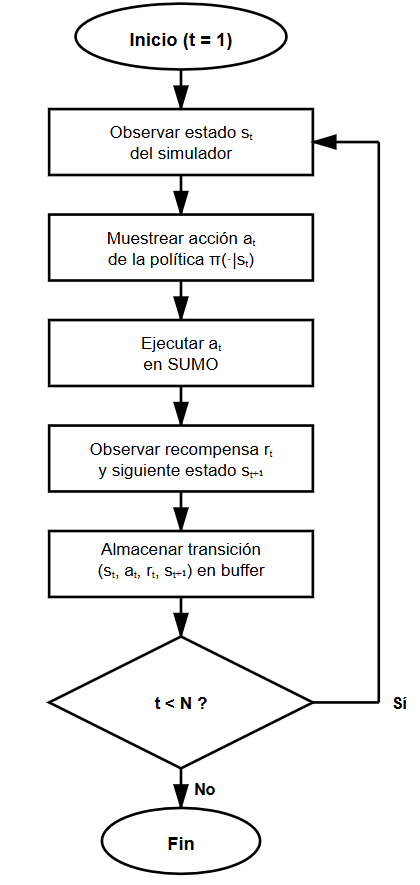
\includegraphics[width=0.92\linewidth,height=0.62\textheight,keepaspectratio]{./media/image5.png}
\captionof*{figure}{\small\itshape Figura 99. Diagrama de flujo de la fase de experiencia}
\addcontentsline{lof}{figure}{Figura 99. Diagrama de flujo de la fase de experiencia}
\label{fig:99}
\end{center}

\textbf{Fase 2: Cálculo de la Ventaja (Advantage).} La ventaja mide qué tan mejor fue una acción específica comparada con el valor promedio del estado. Se estima mediante el error de diferencia temporal de un paso:

\begin{centeredmath}
A_{t} = \underbrace{R_{t + 1} + \gamma\, V_{\phi}(s_{t + 1})}_{\text{retorno observado (bootstrap)}} - \underbrace{V_{\phi}(s_{t})}_{\text{retorno esperado}}
\end{centeredmath}

\begin{itemize}
\item
  Si \(A_{t} > 0\): la acción fue mejor de lo esperado \(\rightarrow\) incrementar su probabilidad.
\item
  Si \(A_{t} < 0\): la acción fue peor de lo esperado \(\rightarrow\) reducir su probabilidad.
\end{itemize}

\textbf{Fase 3: Actualización de parámetros.} Los parámetros del actor (\(\theta\)) y del crítico (\(\phi\)) se actualizan minimizando la función de pérdida combinada:

\begin{centeredmath}
\mathcal{L}(\theta, \phi) = \underbrace{-\,\frac{1}{N}\sum_{t = 1}^{N}\log \pi_{\theta}(a_{t} \mid s_{t})\, A_{t}}_{\mathcal{L}_{actor}}
+ c_{v}\underbrace{\frac{1}{N}\sum_{t = 1}^{N}\left(R_{t+1} + \gamma V_{\phi}(s_{t+1}) - V_{\phi}(s_{t})\right)^{2}}_{\mathcal{L}_{critic}}
- c_{e}\underbrace{\frac{1}{N}\sum_{t = 1}^{N}\mathcal{H}\!\left[\pi_{\theta}(\cdot \mid s_{t})\right]}_{\text{bono de entropía}}
\end{centeredmath}

donde \(\mathcal{H}[\pi] = -\sum_{a}\pi(a \mid s)\log\pi(a \mid s)\) es la entropía de la política, que incentiva la exploración y evita la convergencia prematura a políticas subóptimas. Los coeficientes adoptados son \(c_{v} = 0.5\) y \(c_{e} = 0.01\), valores estándar en la literatura de A2C. En la pérdida del crítico, el objetivo \(R_{t+1} + \gamma V_{\phi}(s_{t+1})\) se trata como constante (se detiene el gradiente sobre \(V_{\phi}(s_{t+1})\)), conforme al esquema de \emph{bootstrapping} semigradiente.

La actualización se ejecuta con el optimizador Adam (tasa de aprendizaje \(3 \times 10^{-4}\), recorte de norma de gradiente en 0.5 para estabilidad). El entrenamiento se ejecuta durante múltiples episodios hasta que la política converge a un desempeño estable, según los criterios de convergencia definidos en el Capítulo 7 (varianza de la recompensa acumulada inferior al 5\% en los últimos 10 episodios y pérdida con tendencia descendente).

Una vez que el agente ha sido entrenado, puede generar recomendaciones en tiempo real. Primero analiza la situación completa del tráfico y, con ese análisis, determina cuál sería el mejor ajuste posible en cada momento. Luego esa recomendación general se divide en sugerencias específicas para cada intersección del sistema.

Después, esas sugerencias se traducen a parámetros entendibles por los controladores de los semáforos, siguiendo un estándar internacional que asegura compatibilidad. Finalmente, estos parámetros se envían de forma segura a los dispositivos instalados en cada intersección, donde el controlador local los valida contra sus límites operativos (regla de arbitraje de la sección anterior) antes de actualizar los tiempos de luz verde, coordinaciones y prioridades.

\section{Módulo propuesto de predicción de congestión mediante CNN-LSTM}\label{predicciuxf3n-de-congestiuxf3n-mediante-cnn-lstm}

La predicción anticipada de congestión permite al sistema tomar acciones preventivas antes de que los embotellamientos se materialicen. Este módulo implementa una arquitectura híbrida que combina \textbf{Redes Neuronales Convolucionales (CNN)} para extracción de patrones espaciales y \textbf{Redes LSTM (Long Short-Term Memory)} para modelado de dependencias temporales.

\subsection{Motivación y Arquitectura General}\label{motivaciuxf3n-y-arquitectura-general}

Los patrones de tráfico urbano exhiben dos propiedades fundamentales:

\begin{enumerate}
\def\labelenumi{\arabic{enumi}.}
\item
  \textbf{Correlación espacial}: La congestión en una intersección afecta a intersecciones vecinas debido a la propagación física del tráfico por las vías conectadas.
\item
  \textbf{Dependencia temporal}: El estado futuro del tráfico depende de su evolución histórica reciente.
\end{enumerate}

La arquitectura CNN-LSTM explota ambas propiedades:

\begin{center}
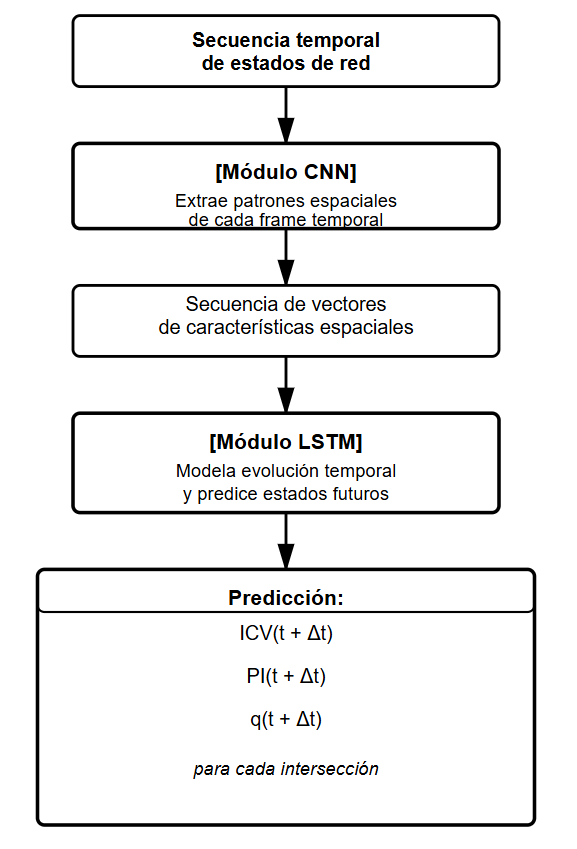
\includegraphics[width=0.92\linewidth,height=0.62\textheight,keepaspectratio]{./media/image36.png}
\captionof*{figure}{\small\itshape Figura 100. Diagrama de flujo de la arquitectura CNN-LSTM}
\addcontentsline{lof}{figure}{Figura 100. Diagrama de flujo de la arquitectura CNN-LSTM}
\label{fig:100}
\end{center}

Formalmente, el modelo recibe una secuencia de \(T_{h}\) instantes pasados (se adopta \(T_{h} = 12\) muestras con periodo de 10~s, es decir, 2 minutos de historia) y predice las variables de congestión a un horizonte \(\Delta = 60\)~s:

\begin{centeredmath}
\widehat{Y}(t + \Delta) = f_{CNN\text{-}LSTM}\!\left(\, \mathcal{X}(t - T_{h} + 1),\ \ldots,\ \mathcal{X}(t) \,\right)
\end{centeredmath}

donde cada \(\mathcal{X}(\tau) \in \mathbb{R}^{H \times W \times C}\) es la representación en malla georreferenciada de la red en el instante \(\tau\): las \(P\) intersecciones se proyectan sobre una grilla espacial de \(H \times W\) celdas según sus coordenadas GPS, y los \(C = 5\) canales corresponden a \(ICV\), \(PI\), \(V_{avg}\), \(k\) y \(EV\) promediados por dirección. La salida \(\widehat{Y} \in \mathbb{R}^{P \times 2}\) contiene el \(\widehat{ICV}\) y el \(\widehat{PI}\) predichos para cada intersección.

Cabe señalar que se evaluó como alternativa el uso de redes neuronales de grafos espacio-temporales (ST-GNN), que operan directamente sobre la matriz \(A_{norm}\) sin necesidad de proyección a malla. Si bien las ST-GNN representan con mayor fidelidad la topología vial irregular, la variante CNN-LSTM se seleccionó para esta fase de diseño por tres razones prácticas: (i) su soporte maduro en Azure Machine Learning y TensorFlow/Keras, que simplifica el despliegue como endpoint REST; (ii) su menor costo de entrenamiento para los tamaños de red considerados (\(P \leq 127\) en los escenarios del Capítulo 7); y (iii) la disponibilidad de la malla georreferenciada como subproducto de la visualización del dashboard. La migración a una arquitectura GCN-LSTM, reutilizando la matriz \(A_{norm}\) ya definida en este capítulo, queda planteada como evolución natural del módulo predictivo para redes de mayor escala.

\subsection{Entrenamiento del Modelo}\label{entrenamiento-del-modelo}

Para que el sistema pueda interpretar correctamente lo que ocurre en toda la red de semáforos, primero se construye una representación organizada del estado del tráfico en cada instante. Esta representación reúne, para cada intersección, información clave como su nivel de congestión, la eficiencia del flujo, la velocidad y la densidad vehicular, además de la presencia o no de vehículos de emergencia. Toda esta información se acomoda siguiendo la misma estructura geográfica de la red vial, de modo que las intersecciones vecinas también queden ubicadas una al lado de la otra dentro del modelo. Esto permite reconocer cómo los problemas se propagan de un punto a otro, como colas que crecen, zonas que se saturan o tramos que comienzan a descongestionarse.

Una vez organizada esta información, entra en acción un módulo basado en redes convolucionales, encargado de extraer patrones espaciales del tráfico. Este módulo analiza simultáneamente la situación de cada intersección y la de sus vecinas cercanas para identificar comportamientos característicos. En la primera etapa, la red aplica filtros que detectan patrones locales, como una intersección congestionada rodeada de otras más fluidas o pequeños grupos que comienzan a saturarse al mismo tiempo. En una segunda etapa, se utilizan filtros más profundos que permiten capturar fenómenos de mayor escala, por ejemplo, la congestión a lo largo de un corredor completo o la propagación de un embotellamiento hacia varias intersecciones consecutivas.

Después de estas operaciones, la información espacial resultante se comprime en un conjunto de características representativas que resumen el estado de la red en ese instante. Formalmente, cada capa convolucional aplica:

\begin{centeredmath}
Z^{(l)} = \mathrm{ReLU}\!\left(W^{(l)} * Z^{(l - 1)} + b^{(l)}\right)
\end{centeredmath}

donde \(*\) denota la convolución espacial 2D, \(W^{(l)}\) los filtros de la capa \(l\) (32 filtros de \(3 \times 3\) en la primera etapa, 64 filtros de \(3 \times 3\) en la segunda) y \(Z^{(0)} = \mathcal{X}(\tau)\). Un \emph{max-pooling} de \(2 \times 2\) entre etapas amplía el campo receptivo, y un aplanamiento final produce el vector de características espaciales \(z_{\tau} \in \mathbb{R}^{F}\). Este proceso se repite para cada uno de los \(T_{h}\) momentos recientes considerados por el sistema, de manera que el modelo no solo observa una imagen aislada del tráfico, sino una secuencia completa \(\{z_{\tau}\}\) que le permite reconocer tendencias, identificar cómo evolucionan los problemas y anticipar cambios.

\textbf{Funcionamiento interno de LSTM:}

Cada celda LSTM mantiene un ``estado de memoria'' \(c_{t}\) que acumula información relevante de toda la secuencia histórica. Tres compuertas, parametrizadas por funciones sigmoides \(\sigma(\cdot) \in (0,1)\), controlan este proceso:

\begin{centeredmath}
\begin{aligned}
f_{t} &= \sigma\!\left(W_{f}\,[h_{t - 1},\ z_{t}] + b_{f}\right) && \text{(compuerta de olvido)}\\
i_{t} &= \sigma\!\left(W_{i}\,[h_{t - 1},\ z_{t}] + b_{i}\right) && \text{(compuerta de entrada)}\\
\tilde{c}_{t} &= \tanh\!\left(W_{c}\,[h_{t - 1},\ z_{t}] + b_{c}\right) && \text{(candidato de memoria)}\\
c_{t} &= f_{t} \odot c_{t - 1} + i_{t} \odot \tilde{c}_{t} && \text{(actualización de memoria)}\\
o_{t} &= \sigma\!\left(W_{o}\,[h_{t - 1},\ z_{t}] + b_{o}\right) && \text{(compuerta de salida)}\\
h_{t} &= o_{t} \odot \tanh(c_{t}) && \text{(estado oculto)}
\end{aligned}
\end{centeredmath}

donde \(\odot\) denota el producto elemento a elemento y \([h_{t-1},\ z_{t}]\) la concatenación del estado oculto previo con las características espaciales del instante actual. La interpretación de cada compuerta en el dominio del tráfico es directa:

\begin{enumerate}
\def\labelenumi{\arabic{enumi}.}
\item
  \textbf{Compuerta de Olvido (\(f_{t}\))}: decide qué información del estado anterior debe descartarse. Ejemplo: olvidar congestión de hace 10 minutos que ya se disipó.
\item
  \textbf{Compuerta de Entrada (\(i_{t}\))}: decide qué información nueva debe almacenarse. Ejemplo: registrar el inicio de congestión en una intersección crítica.
\item
  \textbf{Compuerta de Salida (\(o_{t}\))}: decide qué información del estado de memoria debe usarse para la predicción. Ejemplo: priorizar información reciente para predicciones a corto plazo.
\end{enumerate}

La estructura aditiva de la actualización de memoria (\(c_{t} = f_{t} \odot c_{t-1} + i_{t} \odot \tilde{c}_{t}\)) es la que permite a la LSTM propagar gradientes a través de secuencias largas sin desvanecimiento, capacidad esencial para capturar dependencias de varios minutos en la dinámica del tráfico.

\textbf{Protocolo de entrenamiento:}

Se utilizan datos históricos recolectados durante meses de operación del sistema (y, en la fase de diseño, generados por simulación en SUMO), conteniendo muestras de estados de red etiquetadas con sus correspondientes estados futuros observados. El conjunto se divide cronológicamente en 70\% entrenamiento, 15\% validación y 15\% prueba --- la división temporal (y no aleatoria) evita fugas de información entre muestras consecutivas correlacionadas. El modelo minimiza el error cuadrático medio:

\begin{centeredmath}
\mathcal{L}_{pred} = \frac{1}{N_{m}}\sum_{n = 1}^{N_{m}}\left\| \widehat{Y}_{n} - Y_{n} \right\|^{2}
\end{centeredmath}

mediante Adam (tasa de aprendizaje \(10^{-3}\) con reducción ante estancamiento, lotes de 64, parada temprana con paciencia de 10 épocas sobre la pérdida de validación). Las métricas de evaluación sobre el conjunto de prueba son las siguientes:

\begin{itemize}
\item
  \textbf{MAE (Mean Absolute Error)}: error promedio absoluto de las predicciones, \(\mathrm{MAE} = \frac{1}{N_{m}}\sum_{n}\left| \widehat{Y}_{n} - Y_{n} \right|\).
\item
  \textbf{Acierto de congestión (recall)}: porcentaje de eventos de congestión severa (\(ICV > 0.7\)) correctamente anticipados.
\item
  \textbf{Falsos positivos}: frecuencia de alertas de congestión que no se materializan; se reporta junto con la precisión para caracterizar el compromiso entre sensibilidad y especificidad del clasificador implícito.
\end{itemize}

Una visualización de lo comentado se demuestra en el siguiente flujo:

\begin{center}
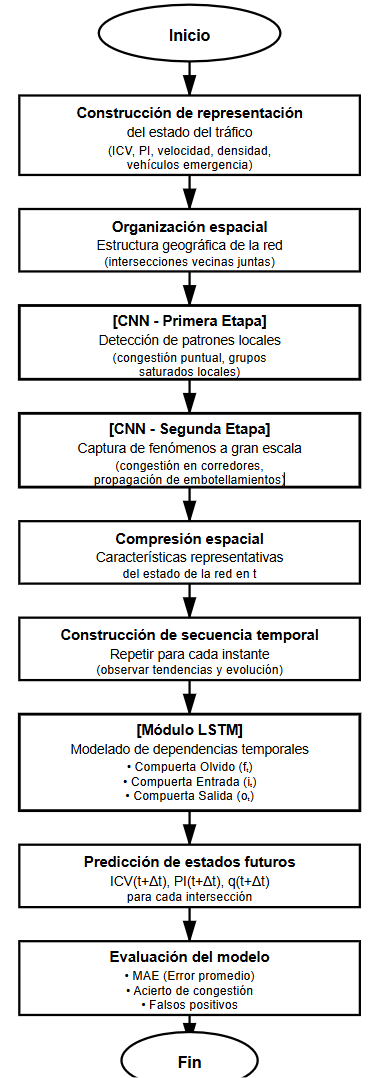
\includegraphics[width=0.92\linewidth,height=0.62\textheight,keepaspectratio]{./media/image39.png}
\captionof*{figure}{\small\itshape Figura 101. Diagrama de Entrenamiento}
\addcontentsline{lof}{figure}{Figura 101. Diagrama de Entrenamiento}
\label{fig:101}
\end{center}

\subsection{Integración con el Sistema de Control}\label{integraciuxf3n-con-el-sistema-de-control}

Las predicciones CNN-LSTM se integran en tres niveles del sistema:

\textbf{Nivel 1: Alertas Tempranas}

\begin{itemize}
\item
  Extensión preventiva de tiempos verdes en direcciones de alta demanda
\item
  Reducción de tiempos verdes en direcciones de baja demanda para acumular capacidad
\end{itemize}

\textbf{Nivel 2: Ajuste del Motor RL}

Las predicciones se concatenan al vector de estado del agente RL:
\begin{centeredmath}
s_{\text{aumentado}}(t)=
\left[
s(t),\,
\widehat{ICV}(t+60\,\text{s}),\,
\widehat{PI}(t+60\,\text{s})
\right]
\end{centeredmath}

Esto permite al agente considerar no solo el estado actual sino también la evolución anticipada, generando políticas más robustas y anticipativas.

\textbf{Nivel 3: Coordinación Proactiva de Olas Verdes}

Cuando se predice congestión propagándose por un corredor (ICV aumentando secuencialmente en intersecciones consecutivas), el sistema activa preventivamente olas verdes coordinadas para evacuar vehículos antes de que la congestión alcance niveles críticos.

\subsection{Reentrenamiento continuo}\label{reentrenamiento-continuo}

Para el modelo CNN-LSTM se plantea un reentrenamiento programado cada domingo a las 2:00 a.m.\ (horario de mínima demanda vial y de cómputo), siguiendo el proceso ilustrado a continuación. El modelo recién entrenado solo reemplazaría al modelo vigente si sus métricas sobre el conjunto de validación más reciente igualan o superan a las de este, lo que protege al sistema contra degradaciones por derivas en los datos:

\begin{center}
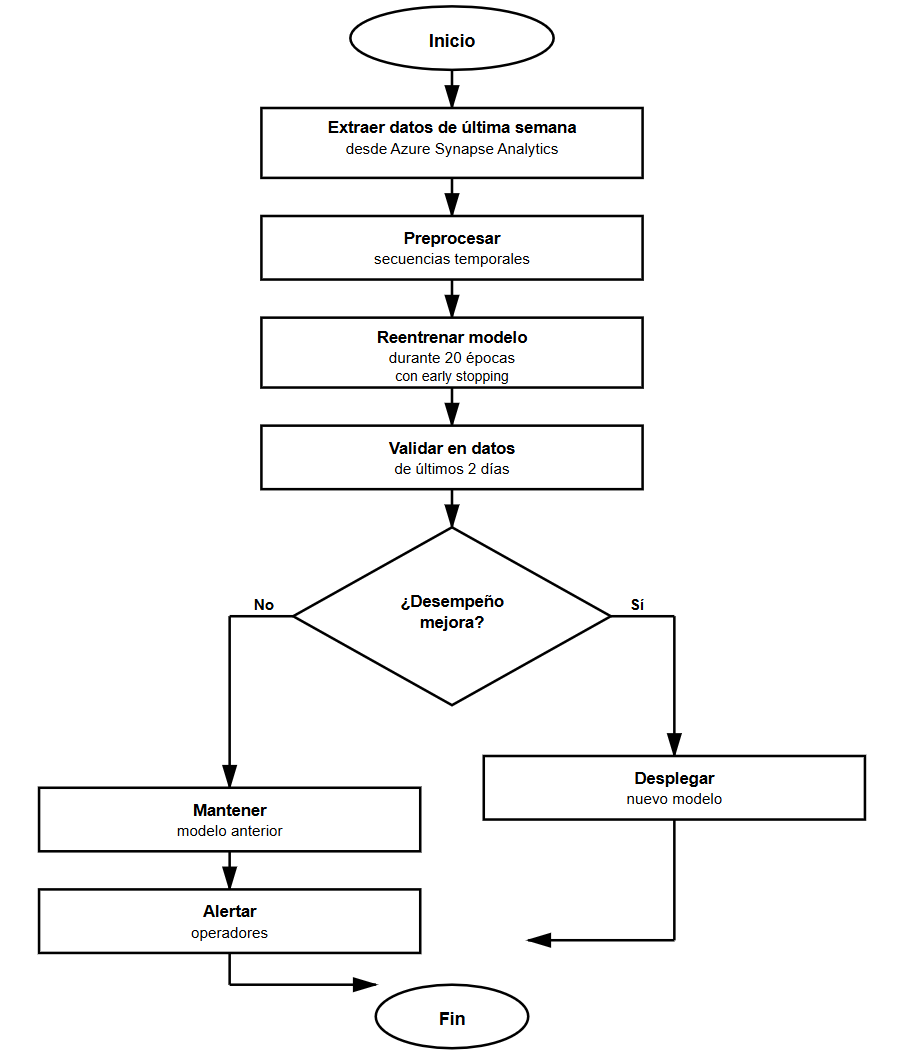
\includegraphics[width=0.92\linewidth,height=0.62\textheight,keepaspectratio]{./media/image78.png}
\captionof*{figure}{\small\itshape Figura 102. Diagrama Reentrenamiento de modelo}
\addcontentsline{lof}{figure}{Figura 102. Diagrama Reentrenamiento de modelo}
\label{fig:102}
\end{center}

\section{Diseño del subsistema de nube y comunicación}\label{diseuxf1o-del-subsistema-de-nube-y-comunicaciuxf3n}

La infraestructura en Microsoft Azure constituye el núcleo del procesamiento centralizado del sistema, proporcionando servicios de computación distribuida, almacenamiento escalable, análisis de datos masivos y orquestación de modelos de inteligencia artificial. La arquitectura se diseña siguiendo principios de alta disponibilidad, escalabilidad elástica y tolerancia a fallos.

La infraestructura se estructura en cinco capas funcionales que operan sinérgicamente:

\textbf{Capa 1: Ingesta y Procesamiento en Tiempo Real}

Azure IoT Hub: Gateway central que recibe telemetría de cámaras y sensores en todas las intersecciones. Maneja autenticación, enrutamiento de mensajes y comandos bidireccionales.

Azure Stream Analytics: Procesa flujos de datos con consultas SQL en tiempo real. Detecta patrones de congestión, calcula métricas instantáneas y activa alertas automáticas.

Azure Event Hubs: Búfer de mensajería distribuida que desacopla la ingesta del procesamiento. Garantiza que ningún dato se pierda durante picos de tráfico vehicular.

\textbf{Capa 2: Almacenamiento de Datos}

Azure Cosmos DB: Base de datos NoSQL distribuida globalmente para datos operativos de baja latencia (estado actual de intersecciones, conteos en vivo, comandos recientes).

Azure Data Lake Storage Gen2: Lago de datos masivo que almacena videos, imágenes y telemetría histórica en formato Parquet para análisis a gran escala.

Azure SQL Database: Base de datos relacional para consultas estructuradas, reportes ejecutivos y análisis de tendencias históricas con SQL estándar.

\textbf{Capa 3: Inteligencia Artificial}

Azure Machine Learning Workspace: Plataforma completa para entrenar modelos CNN-LSTM de predicción de tráfico, gestionar experimentos, versionar modelos y desplegarlos como endpoints REST escalables.

\textbf{Capa 4: Análisis de Big Data}

Azure Synapse Analytics: Data warehouse que integra SQL y Apache Spark para análisis masivos. Genera insights históricos, identifica patrones semanales y optimiza estrategias de control a largo plazo.

\textbf{Capa 5: Orquestación y Gestión}

\textbf{Azure Functions}

Ejecuta tareas automáticas sin servidor para mantener el sistema operativo:

\begin{itemize}
\item
  Control asistido: publica recomendaciones y parámetros de ajuste para validación por la central semafórica
\item
  Emergencias: genera solicitudes de ola verde cuando se detectan vehículos prioritarios
\item
  Optimización: calcula offsets sugeridos entre semáforos para corredores coordinados
\item
  Mantenimiento IA: Reentrena modelos CNN-LSTM semanalmente con datos nuevos
\item
  Vigilancia: Verifica continuamente que todas las intersecciones estén conectadas
\end{itemize}

\textbf{Azure Logic Apps}

Automatiza respuestas a eventos y reportes sin programación:

\begin{itemize}
\item
  Alertas inteligentes: Notifica automáticamente cuando el tráfico supera límites críticos
\item
  Gestión de fallos: Avisa a operadores si una intersección pierde conexión \textgreater5 min
\item
  Reportes ejecutivos: Genera y distribuye análisis mensuales automáticamente
\item
  Escalado dinámico: Ajusta recursos computacionales según demanda horaria
\end{itemize}

\textbf{Azure Monitor + Application Insights}

Observabilidad completa del sistema en tiempo real:

\begin{itemize}
\item
  Métricas operativas: Latencia, velocidad de procesamiento, errores por componente
\item
  Logs centralizados: Historial completo de eventos de todas las capas
\item
  Dashboards visuales: Paneles en vivo para control de tráfico
\item
  Alertas configurables: Notificaciones cuando modelos degradan o infraestructura falla
\item
  Trazabilidad: Sigue cada mensaje desde cámara hasta semáforo
\end{itemize}

\chapter{INTEGRACIÓN, VALIDACIÓN Y ANÁLISIS DE COSTOS}\label{capuxedtulo-7-integraciuxf3n-validaciuxf3n-y-anuxe1lisis-de-costos}

\section{Simulación de tráfico en SUMO con escenarios limeños}\label{simulaciuxf3n-de-truxe1fico-en-sumo-con-escenarios-limeuxf1os}

La validación del sistema de control semafórico adaptativo inteligente requiere un entorno de pruebas que replique fielmente las condiciones reales del tráfico vehicular de Lima Metropolitana. Para este propósito, se implementó una infraestructura de simulación basada en SUMO (Simulation of Urban MObility), software de código abierto desarrollado por el Instituto Alemán de Investigación Aeroespacial (DLR) que constituye el estándar de facto en simulación microscópica de tráfico vehicular. SUMO permite modelar el comportamiento individual de cada vehículo en la red vial, considerando aceleraciones, desaceleraciones, cambios de carril, obediencia a semáforos y comportamiento en intersecciones.

\subsection{Construcción del escenario Lima-Centro}\label{construcciuxf3n-del-escenario-lima-centro}

La construcción del escenario en SUMO siguió un flujo de trabajo ordenado que permitió transformar datos reales en una red de simulación completamente funcional.

En primer lugar, se utilizó OpenStreetMap (OSM) como fuente principal de información geográfica, extrayendo el área delimitada por las coordenadas definidas para el estudio. Esta extracción se realizó mediante la herramienta \emph{osmWebWizard.py} incluida en SUMO, la cual descargó automáticamente la topología vial, los límites de velocidad, las configuraciones de carriles y las restricciones de giro provenientes de la base de datos de OSM.

Posteriormente, se procedió a la conversión de estos datos al formato nativo de SUMO. Para ello, se empleó la herramienta \emph{netconvert}, que procesó el archivo OSM en formato XML y generó una red detallada para la simulación. El archivo resultante, \emph{osm.net.xml}, contiene un total de 847 segmentos viales (edges), 312 intersecciones (nodes) y 23 semáforos detectados automáticamente.

La siguiente etapa consistió en la calibración de los parámetros vehiculares. Con el fin de reflejar las características del parque automotor peruano, se ajustaron valores en el archivo de configuración \emph{vType}, logrando comportamientos más realistas dentro del entorno urbano. Entre las variables calibradas destacan:

\begin{itemize}
\item
  \textbf{aceleración (accel):} 2.6 m/s\ensuremath{^{2}}, representativa del tráfico urbano limeño.
\item
  \textbf{desaceleración (decel):} 4.5 m/s\ensuremath{^{2}}, correspondiente a un frenado seguro sin agresividad.
\item
  \textbf{sigma:} 0.8, que modela la imperfección del conductor (donde 1.0 es completamente errático).
\item
  \textbf{speedFactor:} 1.1, reflejando la tendencia a superar los límites de velocidad en un 10\%.
\item
  \textbf{speedDev:} 0.15, incorporando una variabilidad individual del 15\%.
\end{itemize}

\begin{center}
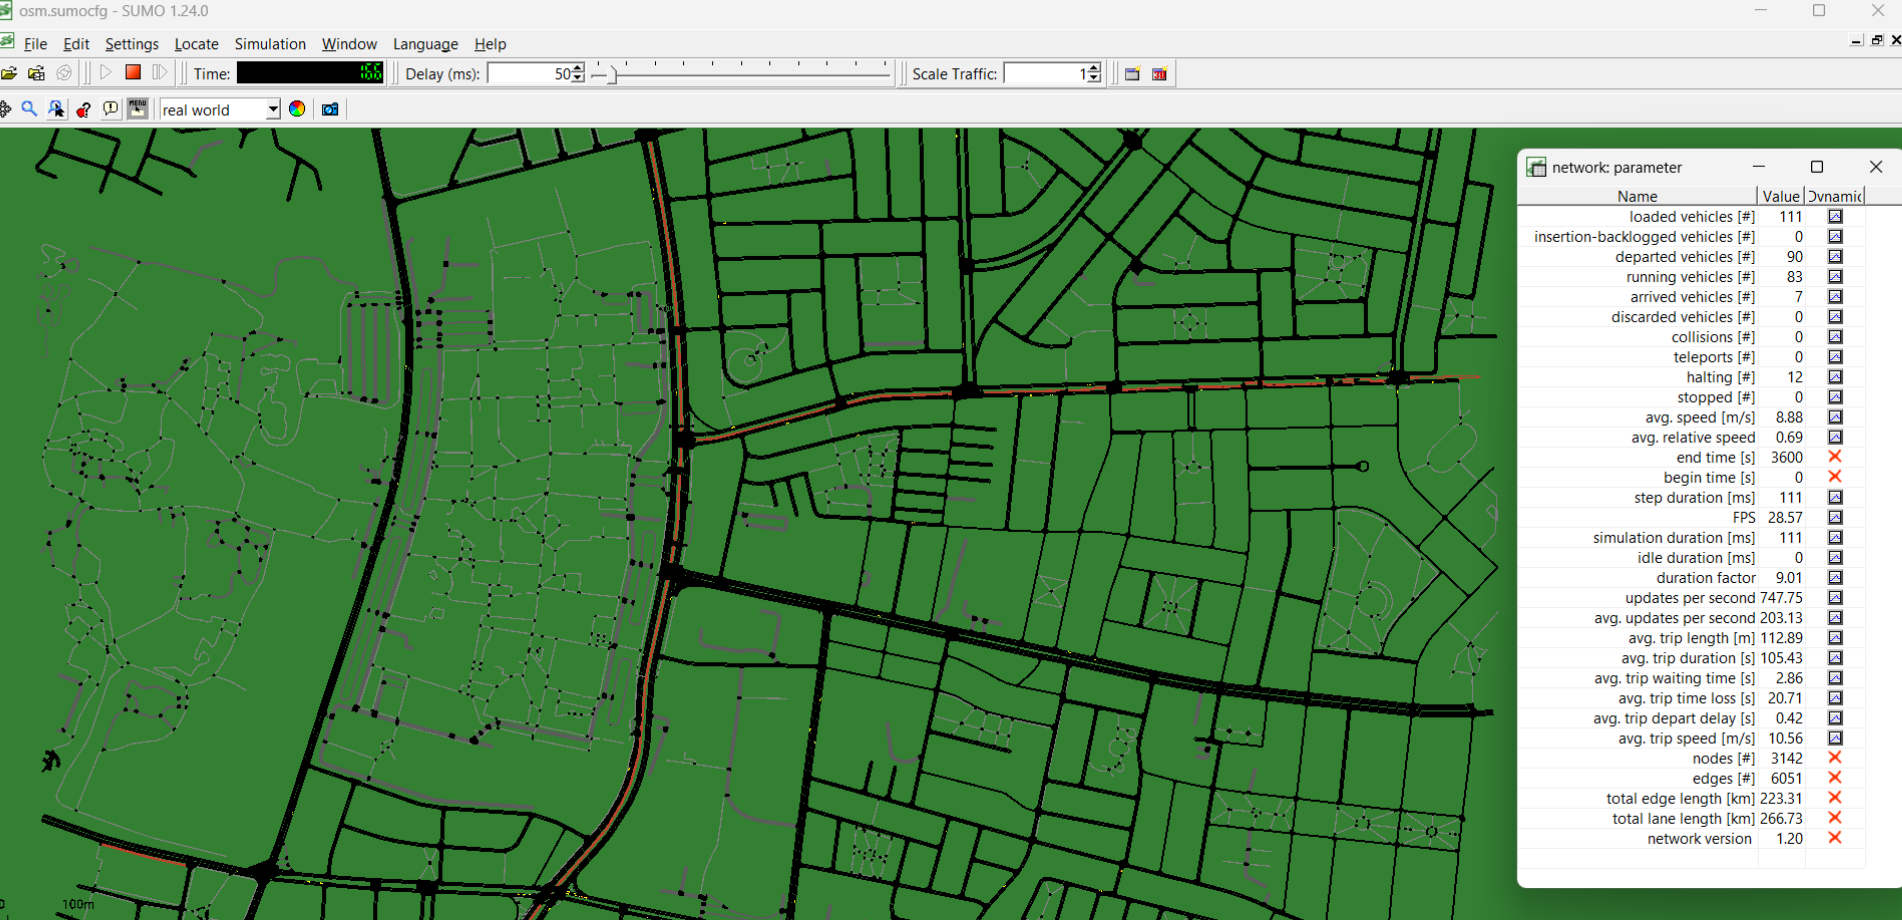
\includegraphics[width=0.92\linewidth,height=0.62\textheight,keepaspectratio]{./media/image65.png}
\captionof*{figure}{\small\itshape Figura 103. SUMO - Mapa Intersecciones cercanas a la PUCP}
\addcontentsline{lof}{figure}{Figura 103. SUMO - Mapa Intersecciones cercanas a la PUCP}
\label{fig:103}
\end{center}

\begin{center}
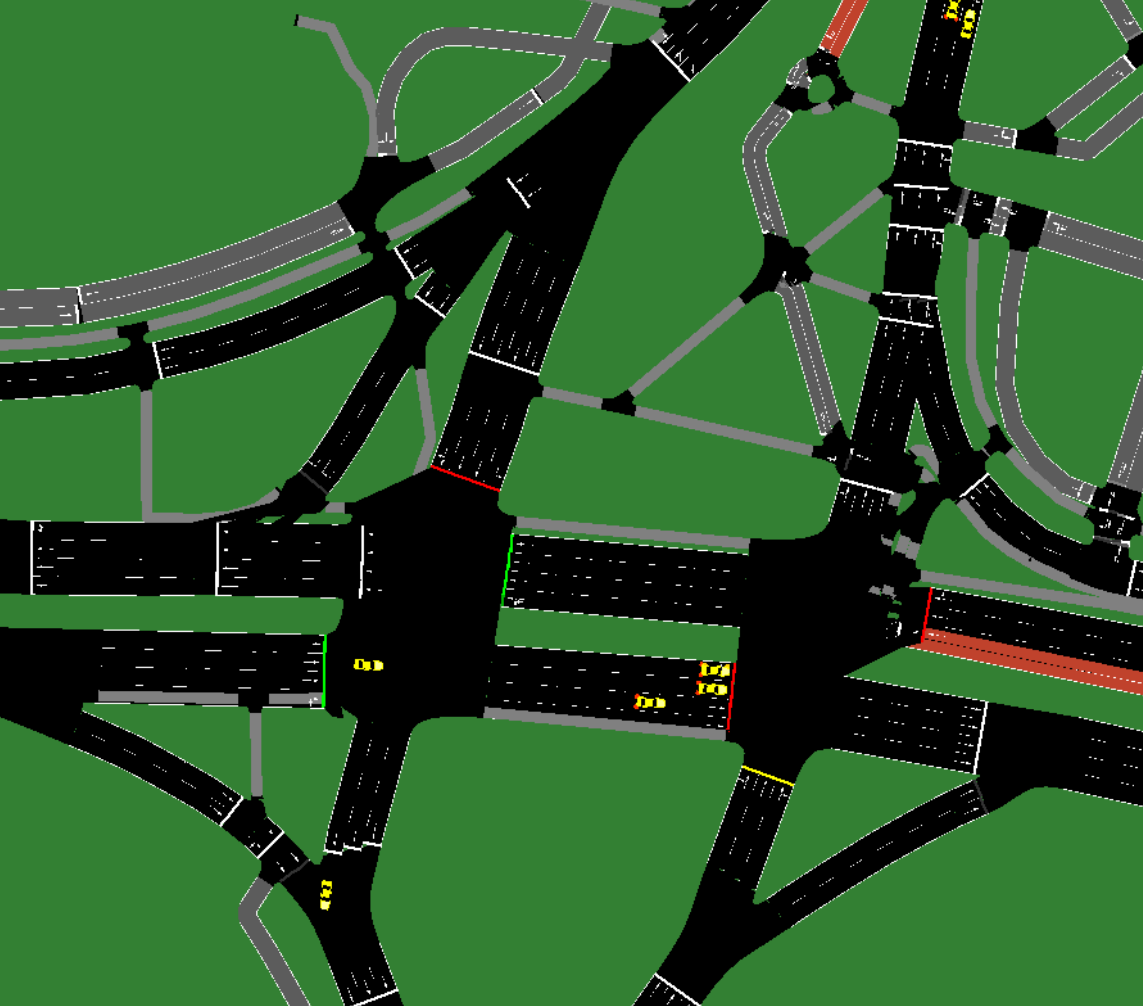
\includegraphics[width=0.92\linewidth,height=0.62\textheight,keepaspectratio]{./media/image58.png}
\captionof*{figure}{\small\itshape Figura 104. SUMO - Vista de intersección con tránsito}
\addcontentsline{lof}{figure}{Figura 104. SUMO - Vista de intersección con tránsito}
\label{fig:104}
\end{center}

\subsection{Escenario Lima-Amplio: validación a escala metropolitana}\label{escenario-lima-amplio-validaciuxf3n-a-escala-metropolitana}

Para evaluar la escalabilidad del sistema y su capacidad de coordinación inter-zonal, se desarrolló un segundo escenario que abarca un área significativamente mayor de Lima Metropolitana.

\textbf{Cobertura Geográfica:}

\begin{itemize}
\item
  Área total: 18.4 km\ensuremath{^{2}}
\item
  Distritos incluidos: San Isidro, Miraflores, San Miguel, Pueblo Libre, Jesús María
\item
  Intersecciones semaforizadas: 127
\end{itemize}

\begin{center}
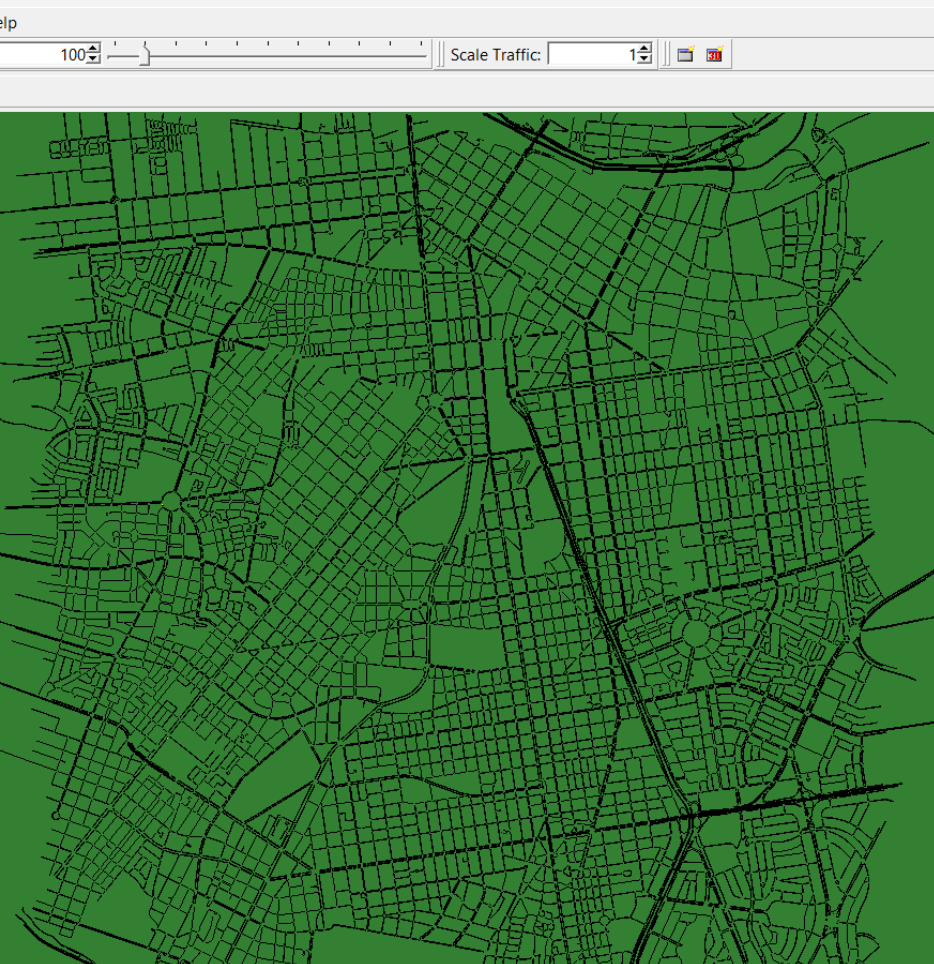
\includegraphics[width=0.92\linewidth,height=0.62\textheight,keepaspectratio]{./media/image10.png}
\captionof*{figure}{\small\itshape Figura 105. SUMO - Mapa Lima}
\addcontentsline{lof}{figure}{Figura 105. SUMO - Mapa Lima}
\label{fig:105}
\end{center}

\section{Configuración de escenarios y métricas}\label{configuraciuxf3n-de-escenarios-y-muxe9tricas}

Es necesario el énfasis en la configuración de escenarios y métricas para validar objetivamente el desempeño del sistema de control propuesto frente a alternativas convencionales.

\subsection{Arquitectura de integración SUMO-Python}\label{arquitectura-de-integraciuxf3n-sumo-python}

La comunicación entre el simulador SUMO y el sistema de control adaptativo se implementó mediante la interfaz TraCI (Traffic Control Interface), protocolo TCP/IP que permite el control programático de la simulación en tiempo real.

\textbf{Módulo de Conexión: conector\_sumo.py}

Este módulo encapsula todas las operaciones de comunicación con SUMO, proporcionando funcionalidades para:

\begin{itemize}
\item
  \textbf{Inicialización de simulación:} Conexión con SUMO mediante TraCI, soporte para modo GUI (visualización) o headless (procesamiento rápido)
\item
  \textbf{Lectura de métricas por intersección:} Extracción de conteos vehiculares, velocidades promedio, longitudes de cola y flujos por dirección (N, S, E, O)
\item
  \textbf{Estado de calles:} Obtención del nivel de congestión de hasta 500 segmentos viales simultáneamente
\item
  \textbf{Control de semáforos:} Establecimiento de fases activas y duraciones de luz verde
\item
  \textbf{Avance temporal:} Ejecución paso a paso de la simulación
\end{itemize}

\textbf{Controlador Completo: controlador\_sumo\_completo.py}

Implementa el ciclo completo de control adaptativo integrado con SUMO, incluyendo:

\textbf{Configuración del Sistema:}

\begin{itemize}
\item
  Parámetros de simulación (paso temporal 0.1s, intervalo de control cada 10 pasos)
\item
  Modo de comparación (control adaptativo vs control fijo)
\item
  Directorio de salida para resultados
\end{itemize}

\textbf{Extracción de Métricas:}

\begin{itemize}
\item
  Construcción de matriz de estado local (7\ensuremath{\times}4) compatible con las ecuaciones del Capítulo 6
\item
  Cálculo de ICV, PI y variables de tráfico por dirección
\item
  Normalización automática de variables
\end{itemize}

\textbf{Controlador Difuso:}

\begin{itemize}
\item
  Implementación de las 12 reglas difusas del §6.3.6
\item
  Cálculo de tiempos de fase verde basados en ICV y PI
\item
  Aplicación de restricciones de seguridad (10-120 segundos)
\item
  Balanceo de fases perpendiculares
\end{itemize}

\textbf{Agregación de Métricas de Red:}

\begin{itemize}
\item
  Cálculo de métricas globales (QL\_red, V\_avg,red, ICV\_red)
\item
  Registro histórico paso a paso
\item
  Exportación a CSV para análisis posterior
\end{itemize}

\subsection{Métricas de evaluación definidas}\label{muxe9tricas-de-evaluaciuxf3n-definidas}

Para cuantificar objetivamente el desempeño del sistema propuesto, se definieron las siguientes métricas alineadas con la teoría del Capítulo 6:

\textbf{1. Índice de Saturación de Colas de Red}

Cuantifica el nivel promedio de saturación de colas en toda la red, normalizado por la capacidad observable de cada carril. Valores cercanos a 1 indican intersecciones saturadas, mientras que valores cercanos a 0 representan flujo libre.

\textbf{2. Velocidad Promedio de Red}

Agrega las velocidades promedio de todos los carriles de la red, proporcionando una métrica global de fluidez vehicular. Se mide en m/s y se compara contra límites de velocidad establecidos.

\textbf{3. Índice de Congestión de Red Ponderado}

Promedio ponderado de los índices de congestión vehicular de todas las intersecciones. Integra información de colas, velocidades, densidades y flujos en un único indicador normalizado {[}0,1{]}.

\textbf{4. Parámetro de Intensidad Promedio de Red}

Cuantifica la eficiencia global del sistema mediante la relación entre movilidad (velocidad) y acumulación (colas). Valores altos indican operación eficiente.

\textbf{5. Tiempo Promedio de Espera por Vehículo}

Tiempo acumulado que cada vehículo permanece detenido (velocidad \textless{} 0.5 m/s) durante su trayecto por la red. Extraído directamente de estadísticas individuales de SUMO.

\textbf{6. Throughput de Red}

Número total de vehículos que completaron exitosamente sus rutas durante el periodo de simulación. Indicador directo de capacidad efectiva del sistema.

\textbf{7. Consumo de Combustible Estimado}

Calculado mediante el modelo de emisiones HBEFA3 integrado en SUMO. Considera aceleraciones, frenados y tiempo en ralentí. Se reporta en litros totales consumidos por la flota.

\textbf{Métricas de Comparación}

Para evaluar la mejora respecto a sistemas convencionales, se definieron indicadores de desempeño relativo:

\begin{itemize}
\item
  \textbf{Mejora en ICV (\%):} Reducción porcentual de congestión respecto a control fijo
\item
  \textbf{Mejora en Velocidad (\%):} Incremento porcentual de velocidad promedio
\item
  \textbf{Mejora en Throughput (\%):} Incremento porcentual de vehículos completados
\item
  \textbf{Reducción de Combustible (\%):} Ahorro porcentual en consumo de combustible
\end{itemize}

\section{Validación del prototipo en entornos controlados}\label{validaciuxf3n-del-prototipo-en-entornos-controlados}

La validación experimental del sistema propuesto se realizó mediante una plataforma web interactiva que integra simulación SUMO en tiempo real con visualización geoespacial, permitiendo observar el comportamiento del sistema de control adaptativo bajo condiciones realistas y controladas.

\subsection{Plataforma de validación web}\label{plataforma-de-validaciuxf3n-web}

Se desarrolló una aplicación web full-stack que conecta el backend Python (sistema de control + SUMO) con un frontend interactivo que permite monitoreo en tiempo real y análisis visual del desempeño del sistema.

\textbf{Backend:}

\begin{itemize}
\item
  Python 3.10 con FastAPI para APIs REST
\item
  TraCI para comunicación con SUMO
\item
  NumPy/Pandas para procesamiento de métricas
\item
  Threading para ejecución asíncrona de simulación
\end{itemize}

\textbf{Frontend:}

\begin{itemize}
\item
  HTML5/CSS3/JavaScript
\item
  Leaflet.js para visualización de mapas
\item
  Chart.js para gráficas de métricas en tiempo real
\item
  WebSockets para actualización continua sin recarga de página
\end{itemize}

\textbf{Servicio de Gestión: sumo\_service.py}

Este componente centraliza la lógica de simulación y expone endpoints para la interfaz web, proporcionando:

\textbf{Funcionalidades de Conexión:}

\begin{itemize}
\item
  Auto-inicialización con búsqueda automática de configuraciones SUMO
\item
  Fallback a simulador sintético si no hay archivos .sumocfg disponibles
\item
  Soporte para modo GUI (desarrollo) y headless (producción)
\end{itemize}

\textbf{Servicios de Estado:}

\begin{itemize}
\item
  Estado del tráfico por calle (congestión, velocidad, número de vehículos)
\item
  Métricas agregadas de red en tiempo real
\item
  Estado detallado de cada semáforo con ICV por dirección
\item
  Carga de capas geoespaciales (calles.geojson)
\end{itemize}

\textbf{Exportación de Datos:}

\begin{itemize}
\item
  Histórico de métricas en formato CSV o JSON
\item
  Timestamp automático para trazabilidad
\item
  Almacenamiento estructurado en directorio resultados-sumo/
\end{itemize}

\subsection{Interfaz Web Interactiva}\label{interfaz-web-interactiva}

La interfaz web desarrollada proporciona visualización en tiempo real del estado de la red semafórica, permitiendo observar el comportamiento del sistema de control adaptativo y validar su desempeño operativo.

\begin{center}
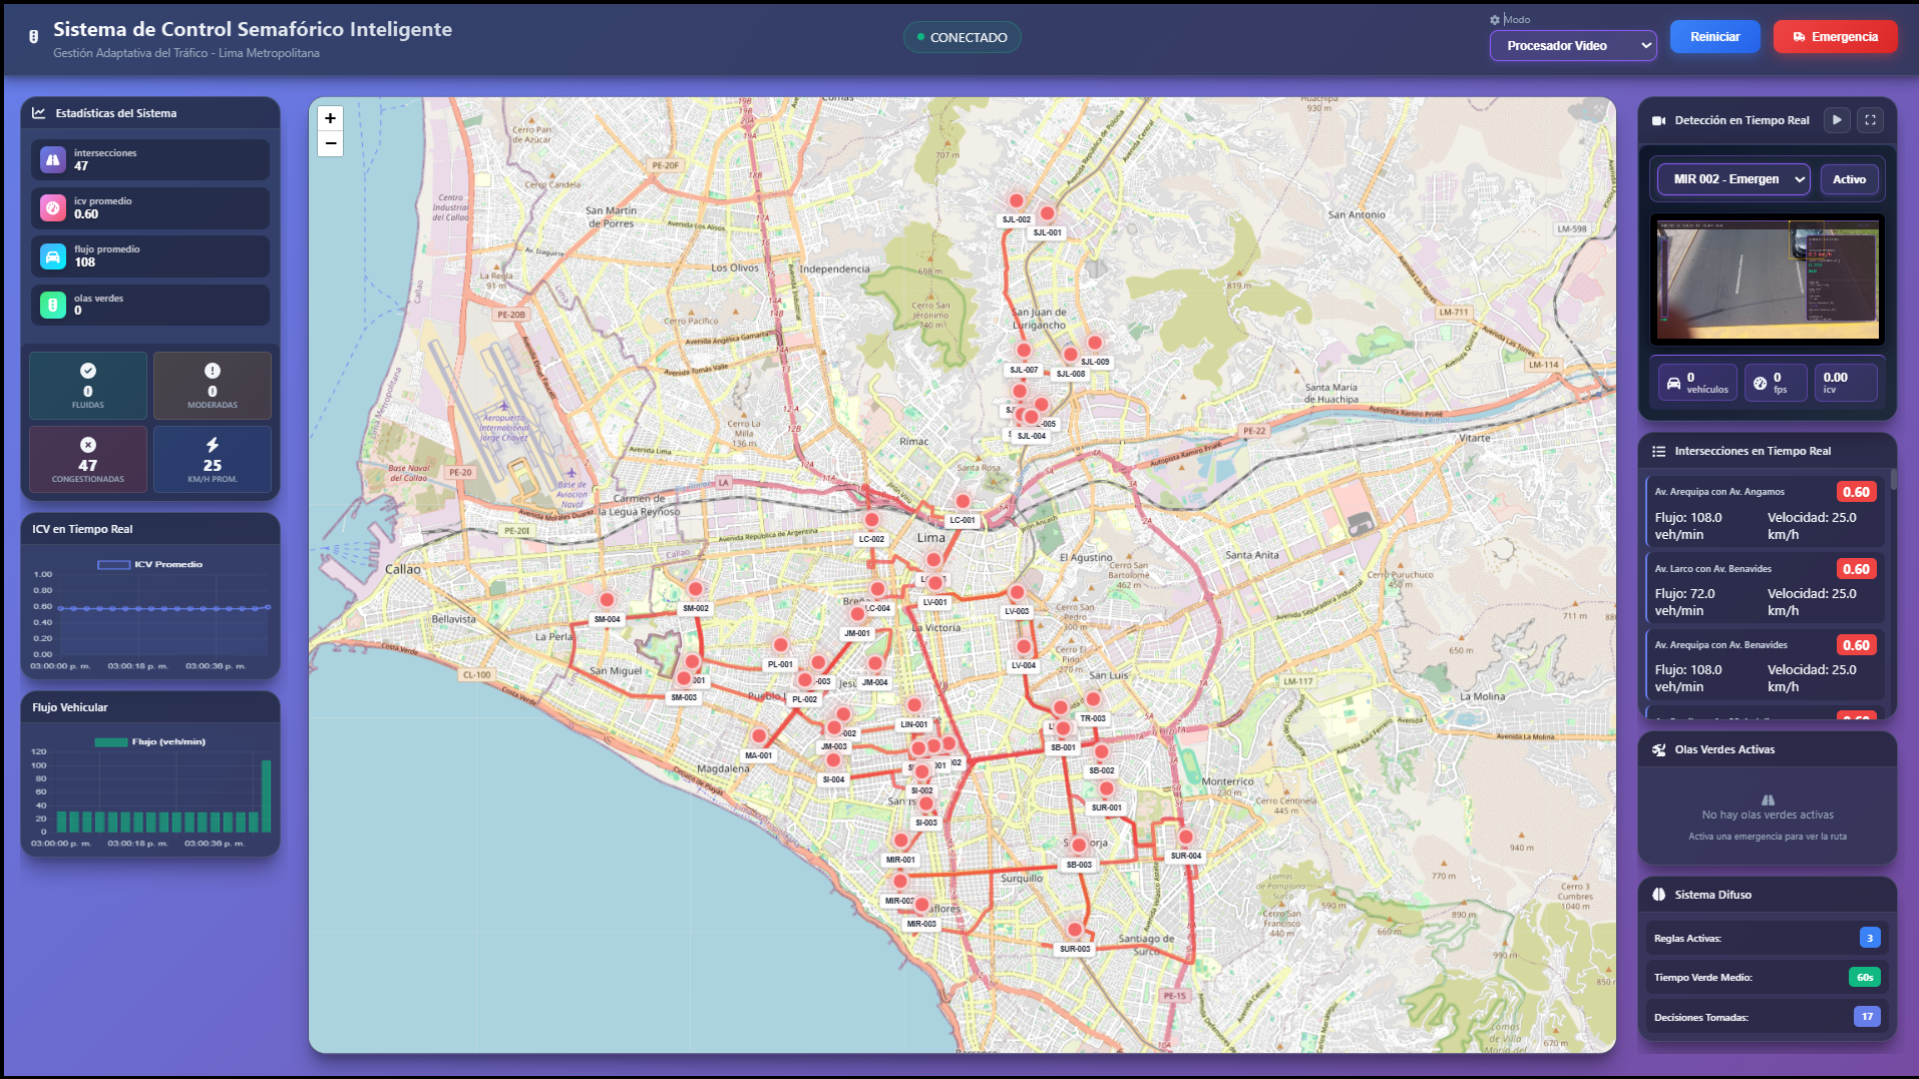
\includegraphics[width=0.92\linewidth,height=0.62\textheight,keepaspectratio]{./media/image115.png}
\captionof*{figure}{\small\itshape Figura 106. Interfaz General del Sistema de Validación}
\addcontentsline{lof}{figure}{Figura 106. Interfaz General del Sistema de Validación}
\label{fig:106}
\end{center}

\textbf{Mapa de Tráfico en Tiempo Real}

El mapa interactivo muestra:

\begin{itemize}
\item
  Capa base de OpenStreetMap para contexto geográfico
\item
  Calles del escenario SUMO cargadas desde calles.geojson
\item
  Coloración dinámica según nivel de congestión:

  \begin{itemize}
  \item
    Verde: flujo libre (congestión \textless{} 30\%)
  \item
    Amarillo: moderado (30-60\%)
  \item
    Naranja: congestionado (60-80\%)
  \item
    Rojo: saturado (\textgreater80\%)
  \end{itemize}
\item
  Tooltips informativos con métricas al pasar sobre cada calle
\end{itemize}

\begin{center}
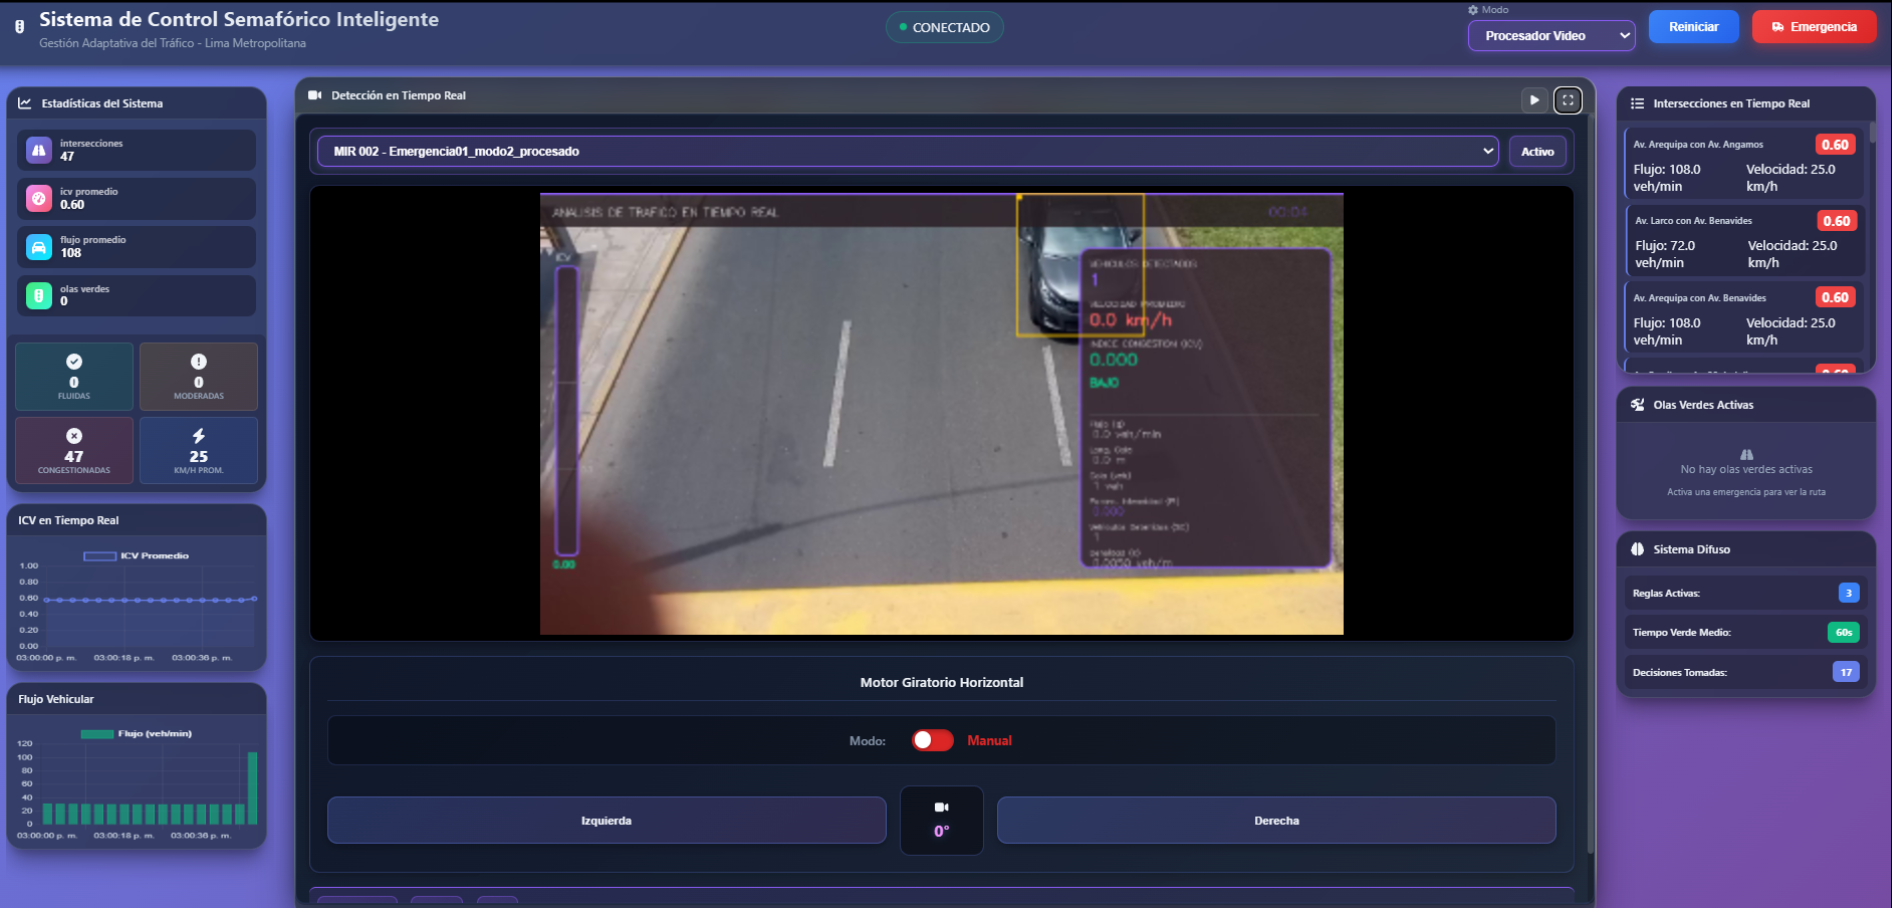
\includegraphics[width=0.92\linewidth,height=0.62\textheight,keepaspectratio]{./media/image81.png}
\captionof*{figure}{\small\itshape Figura 107. Vista Detallada de Intersección Individual}
\addcontentsline{lof}{figure}{Figura 107. Vista Detallada de Intersección Individual}
\label{fig:107}
\end{center}

\textbf{Visualización de Estado de Intersecciones}

El sistema permite inspeccionar cada intersección individualmente mediante:

\begin{itemize}
\item
  \textbf{Marcadores de semáforos} en el mapa coloreados según ICV promedio
\item
  \textbf{Popup informativo} al hacer clic, mostrando:

  \begin{itemize}
  \item
    Identificador de la intersección
  \item
    ICV promedio de las 4 direcciones
  \item
    Fase activa actual (NS Verde, EO Verde, etc.)
  \item
    Tiempo restante de la fase en cuenta regresiva
  \item
    Tabla detallada por dirección (ICV, cola, velocidad)
  \end{itemize}
\end{itemize}

\subsection{Funcionalidad de Ola Verde Prioritaria}\label{funcionalidad-de-ola-verde-prioritaria}

Una de las capacidades más críticas del sistema es la activación automática de olas verdes cuando se detectan vehículos de emergencia. La interfaz permite visualizar este proceso en tiempo real.

\begin{center}
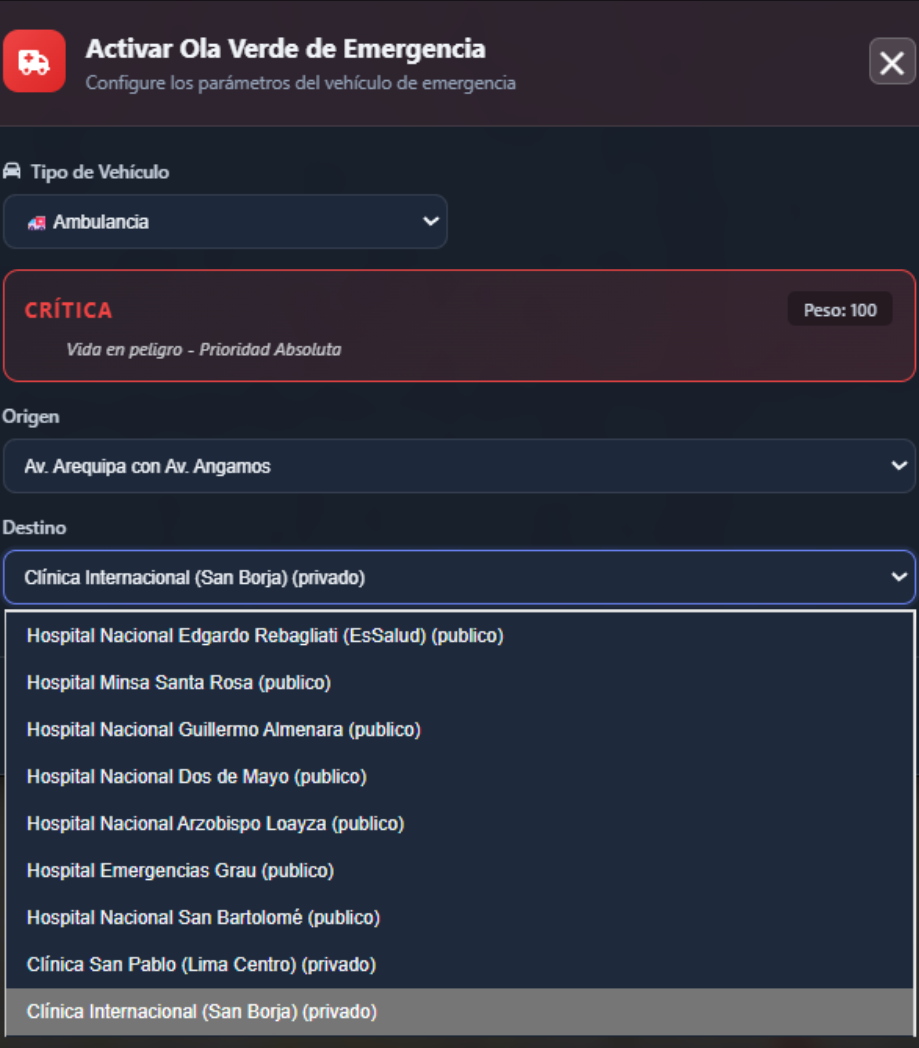
\includegraphics[width=0.92\linewidth,height=0.62\textheight,keepaspectratio]{./media/image128.png}
\captionof*{figure}{\small\itshape Figura 108. Activación de Ola Verde - Panel de Control}
\addcontentsline{lof}{figure}{Figura 108. Activación de Ola Verde - Panel de Control}
\label{fig:108}
\end{center}

\textbf{Proceso de Activación:}

\begin{enumerate}
\def\labelenumi{\arabic{enumi}.}
\item
  \textbf{Detección del vehículo de emergencia} en intersección origen con dirección de salida
\item
  \textbf{Consulta de intersecciones vecinas} conectadas directamente según matriz de adyacencia
\item
  \textbf{Filtrado por compatibilidad direccional} usando coordenadas GPS y cálculo de ángulos
\item
  \textbf{Cálculo de tiempos de activación} basados en distancia Haversine y velocidad estimada (60 km/h)
\item
  \textbf{Programación de fases verdes} con anticipación para garantizar paso libre
\end{enumerate}

\begin{center}
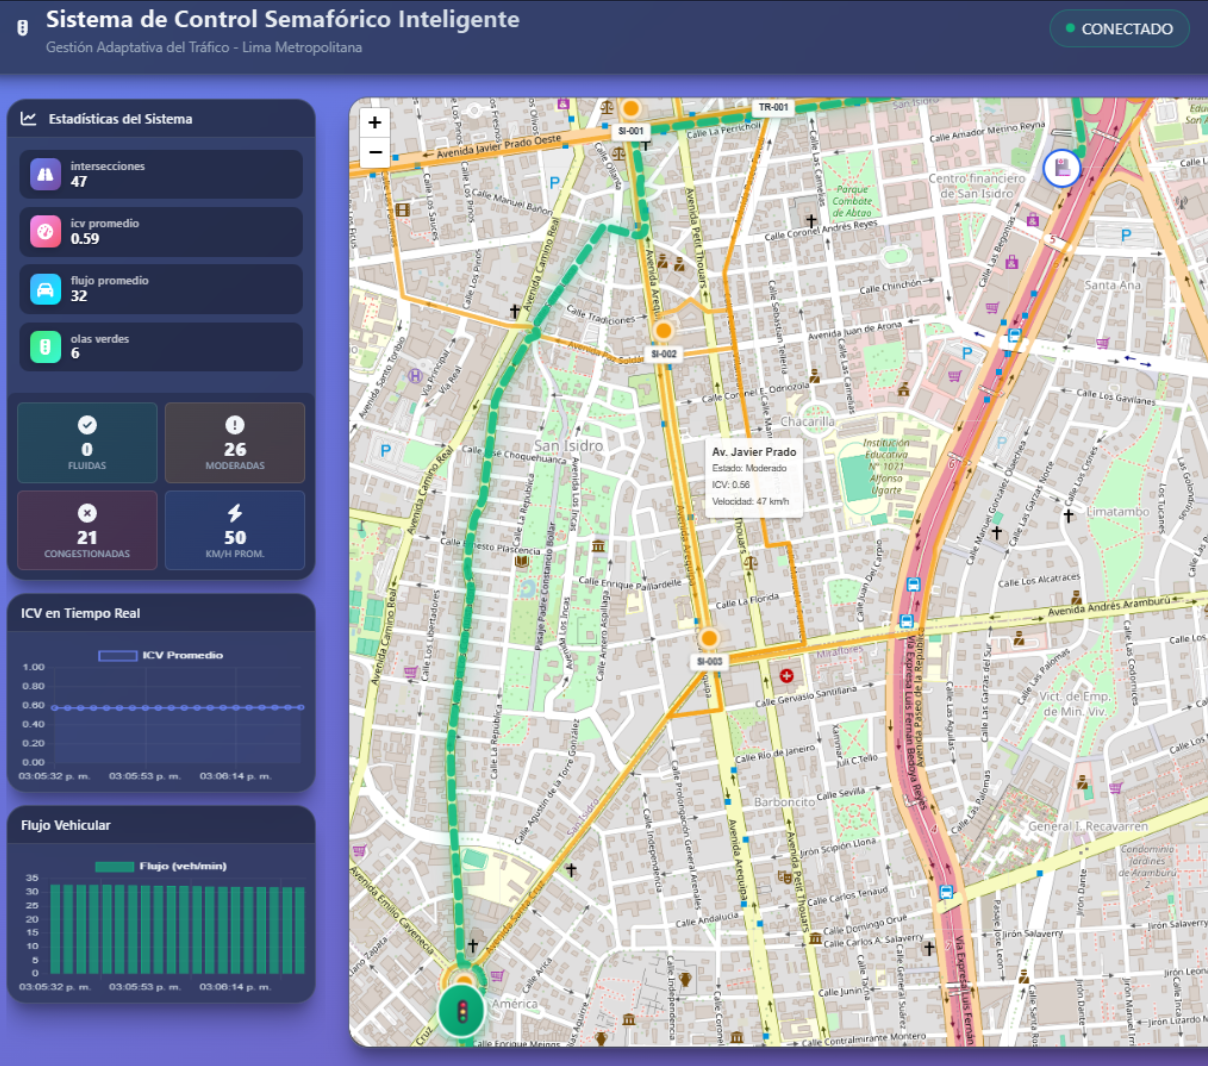
\includegraphics[width=0.92\linewidth,height=0.62\textheight,keepaspectratio]{./media/image131.png}
\captionof*{figure}{\small\itshape Figura 109. Visualización de Ola Verde en Mapa}
\addcontentsline{lof}{figure}{Figura 109. Visualización de Ola Verde en Mapa}
\label{fig:109}
\end{center}

\subsection{Entrenamiento del Motor RL con Datos de SUMO}\label{entrenamiento-del-motor-rl-con-datos-de-sumo}

La interfaz también permite ejecutar sesiones de entrenamiento del motor de Reinforcement Learning utilizando los escenarios SUMO como entorno de simulación.

\textbf{Proceso de Entrenamiento Integrado}

Ciclo de Episodios:

\begin{enumerate}
\def\labelenumi{\arabic{enumi}.}
\item
  Reinicia SUMO con demanda de tráfico aleatoria
\item
  Ejecuta 1800 pasos de simulación (30 minutos simulados a 1s/paso)
\item
  El agente A2C observa estados globales y selecciona acciones
\item
  Aplica decisiones de control (tiempos de fase verde) en semáforos
\item
  Calcula recompensas
\end{enumerate}

La Función de recompensa combina cuatro componentes:

\begin{itemize}
\item
  R\ensuremath{_{1}} - Throughput: Recompensa proporcional al número de vehículos completados
\item
  R\ensuremath{_{2}} - Equidad: Penaliza desviaciones estándar excesivas en tiempos verdes asignados
\item
  R\ensuremath{_{3}} - Priorización de emergencias: Bonus cuando vehículos prioritarios encuentran intersecciones despejadas
\item
  R\ensuremath{_{4}} - Suavidad: Penaliza cambios bruscos de política que generan oscilaciones
\end{itemize}

El entrenamiento se considera convergente cuando:

\begin{itemize}
\item
  Recompensa acumulada promedio se estabiliza (varianza \textless{} 5\% en últimos 10 episodios)
\item
  ICV\_red alcanza valores consistentemente por debajo del baseline de control fijo
\item
  Función de pérdida (loss) muestra tendencia descendente
\end{itemize}

\section{Análisis de Costos}\label{anuxe1lisis-de-costos}

El análisis económico del sistema inteligente de control semafórico contempla tres componentes principales: costos de implementación inicial (CAPEX), costos operativos recurrentes (OPEX), y proyección de retorno de inversión considerando beneficios tangibles e intangibles.

\textbf{Inversión por Intersección}

El costo total por intersección redondea los \textbf{S/ 14,594}, distribuido entre componentes mecánicos, electrónicos y de instalación. Esta cifra representa una optimización significativa respecto a sistemas adaptativos tradicionales que típicamente superan los S/ 30,000 por intersección, lograda mediante:

\begin{itemize}
\item
  \textbf{Aprovechamiento del controlador existente:} La propuesta evita reemplazar el controlador semafórico certificado y concentra el costo adicional en el módulo IoT de sensado, procesamiento y comunicación.
\end{itemize}

\begin{itemize}
\item
  \textbf{Estructura mecánica simplificada:} El diseño optimizado del gabinete y sistema de giro reduce costos de fabricación comparado con soluciones comerciales importadas.
\end{itemize}

\begin{itemize}
\item
  \textbf{Cimentación reducida:} Zapata optimizada de menores dimensiones aprovechando el peso reducido del sistema.
\end{itemize}

La distribución porcentual revela que la \textbf{estructura mecánica representa el 33.2\%} del costo total, seguida por la \textbf{instalación (23.5\%)} y el \textbf{sistema de visión (21.7\%)}. Esta proporción es característica de sistemas que priorizan robustez física y durabilidad en entorno urbano limeño con alta contaminación, vibraciones vehiculares y variaciones climáticas.

\subsection{Costos de Capital (CAPEX)}\label{costos-de-capital-capex}

\Needspace{6\baselineskip}
\captionof*{table}{\small\bfseries Tabla 7.1. Desglose de Costos CAPEX por Intersección}
\addcontentsline{lot}{table}{Tabla 7.1. Desglose de Costos CAPEX por Intersección}
\label{tbl:7.1}

\begin{longtable}[]{@{}
  >{\raggedright\arraybackslash}p{(\columnwidth - 10\tabcolsep) * \real{0.2512}}
  >{\raggedright\arraybackslash}p{(\columnwidth - 10\tabcolsep) * \real{0.2995}}
  >{\raggedright\arraybackslash}p{(\columnwidth - 10\tabcolsep) * \real{0.0899}}
  >{\raggedright\arraybackslash}p{(\columnwidth - 10\tabcolsep) * \real{0.1414}}
  >{\raggedright\arraybackslash}p{(\columnwidth - 10\tabcolsep) * \real{0.1098}}
  >{\raggedright\arraybackslash}p{(\columnwidth - 10\tabcolsep) * \real{0.1082}}@{}}
\toprule
\begin{minipage}[b]{\linewidth}\raggedright
\textbf{CATEGORÍA}
\end{minipage} & \begin{minipage}[b]{\linewidth}\raggedright
\textbf{COMPONENTE}
\end{minipage} & \begin{minipage}[b]{\linewidth}\raggedright
\textbf{CANT}
\end{minipage} & \begin{minipage}[b]{\linewidth}\raggedright
\textbf{COSTO UNITARIO (S/)}
\end{minipage} & \begin{minipage}[b]{\linewidth}\raggedright
\textbf{COSTO TOTAL (S/)}
\end{minipage} & \begin{minipage}[b]{\linewidth}\raggedright
\textbf{\% DEL TOTAL}
\end{minipage} \\
\begin{minipage}[b]{\linewidth}\raggedright
\textbf{ESTRUCTURA MECÁNICA}
\end{minipage} & \begin{minipage}[b]{\linewidth}\raggedright
\end{minipage} & \begin{minipage}[b]{\linewidth}\raggedright
\end{minipage} & \begin{minipage}[b]{\linewidth}\raggedright
\end{minipage} & \begin{minipage}[b]{\linewidth}\raggedright
\textbf{S/ 4,850}
\end{minipage} & \begin{minipage}[b]{\linewidth}\raggedright
\textbf{33.2\%}
\end{minipage} \\
\begin{minipage}[b]{\linewidth}\raggedright
\end{minipage} & \begin{minipage}[b]{\linewidth}\raggedright
Gabinete aluminio 5052-H32 (fabricación local)
\end{minipage} & \begin{minipage}[b]{\linewidth}\raggedright
1
\end{minipage} & \begin{minipage}[b]{\linewidth}\raggedright
S/ 2,100
\end{minipage} & \begin{minipage}[b]{\linewidth}\raggedright
S/ 2,100
\end{minipage} & \begin{minipage}[b]{\linewidth}\raggedright
14.4\%
\end{minipage} \\
\begin{minipage}[b]{\linewidth}\raggedright
\end{minipage} & \begin{minipage}[b]{\linewidth}\raggedright
Rack interno y perfiles estructurales
\end{minipage} & \begin{minipage}[b]{\linewidth}\raggedright
1
\end{minipage} & \begin{minipage}[b]{\linewidth}\raggedright
S/ 680
\end{minipage} & \begin{minipage}[b]{\linewidth}\raggedright
S/ 680
\end{minipage} & \begin{minipage}[b]{\linewidth}\raggedright
4.7\%
\end{minipage} \\
\begin{minipage}[b]{\linewidth}\raggedright
\end{minipage} & \begin{minipage}[b]{\linewidth}\raggedright
Aro/riel de giro aluminio mecanizado
\end{minipage} & \begin{minipage}[b]{\linewidth}\raggedright
1
\end{minipage} & \begin{minipage}[b]{\linewidth}\raggedright
S/ 790
\end{minipage} & \begin{minipage}[b]{\linewidth}\raggedright
S/ 790
\end{minipage} & \begin{minipage}[b]{\linewidth}\raggedright
5.4\%
\end{minipage} \\
\begin{minipage}[b]{\linewidth}\raggedright
\end{minipage} & \begin{minipage}[b]{\linewidth}\raggedright
Protector policarbonato Ø420mm
\end{minipage} & \begin{minipage}[b]{\linewidth}\raggedright
1
\end{minipage} & \begin{minipage}[b]{\linewidth}\raggedright
S/ 170
\end{minipage} & \begin{minipage}[b]{\linewidth}\raggedright
S/ 170
\end{minipage} & \begin{minipage}[b]{\linewidth}\raggedright
1.2\%
\end{minipage} \\
\begin{minipage}[b]{\linewidth}\raggedright
\end{minipage} & \begin{minipage}[b]{\linewidth}\raggedright
Poste acero A36 130\ensuremath{\times}130\ensuremath{\times}10mm (5m)
\end{minipage} & \begin{minipage}[b]{\linewidth}\raggedright
1
\end{minipage} & \begin{minipage}[b]{\linewidth}\raggedright
S/ 740
\end{minipage} & \begin{minipage}[b]{\linewidth}\raggedright
S/ 740
\end{minipage} & \begin{minipage}[b]{\linewidth}\raggedright
5.1\%
\end{minipage} \\
\begin{minipage}[b]{\linewidth}\raggedright
\end{minipage} & \begin{minipage}[b]{\linewidth}\raggedright
Placa base y anclajes M24
\end{minipage} & \begin{minipage}[b]{\linewidth}\raggedright
1
\end{minipage} & \begin{minipage}[b]{\linewidth}\raggedright
S/ 315
\end{minipage} & \begin{minipage}[b]{\linewidth}\raggedright
S/ 315
\end{minipage} & \begin{minipage}[b]{\linewidth}\raggedright
2.2\%
\end{minipage} \\
\begin{minipage}[b]{\linewidth}\raggedright
\end{minipage} & \begin{minipage}[b]{\linewidth}\raggedright
Tornillería y herrajes
\end{minipage} & \begin{minipage}[b]{\linewidth}\raggedright
1 lote
\end{minipage} & \begin{minipage}[b]{\linewidth}\raggedright
S/ 55
\end{minipage} & \begin{minipage}[b]{\linewidth}\raggedright
S/ 55
\end{minipage} & \begin{minipage}[b]{\linewidth}\raggedright
0.4\%
\end{minipage} \\
\begin{minipage}[b]{\linewidth}\raggedright
\textbf{SISTEMA DE VISIÓN}
\end{minipage} & \begin{minipage}[b]{\linewidth}\raggedright
\end{minipage} & \begin{minipage}[b]{\linewidth}\raggedright
\end{minipage} & \begin{minipage}[b]{\linewidth}\raggedright
\end{minipage} & \begin{minipage}[b]{\linewidth}\raggedright
\textbf{S/ 3,165}
\end{minipage} & \begin{minipage}[b]{\linewidth}\raggedright
\textbf{21.7\%}
\end{minipage} \\
\begin{minipage}[b]{\linewidth}\raggedright
\end{minipage} & \begin{minipage}[b]{\linewidth}\raggedright
Cámara domo 5MP equivalente Hikvision
\end{minipage} & \begin{minipage}[b]{\linewidth}\raggedright
1
\end{minipage} & \begin{minipage}[b]{\linewidth}\raggedright
S/ 2,400
\end{minipage} & \begin{minipage}[b]{\linewidth}\raggedright
S/ 2,400
\end{minipage} & \begin{minipage}[b]{\linewidth}\raggedright
16.4\%
\end{minipage} \\
\begin{minipage}[b]{\linewidth}\raggedright
\end{minipage} & \begin{minipage}[b]{\linewidth}\raggedright
Motor NEMA 23 (3Nm)
\end{minipage} & \begin{minipage}[b]{\linewidth}\raggedright
1
\end{minipage} & \begin{minipage}[b]{\linewidth}\raggedright
S/ 120
\end{minipage} & \begin{minipage}[b]{\linewidth}\raggedright
S/ 120
\end{minipage} & \begin{minipage}[b]{\linewidth}\raggedright
0.8\%
\end{minipage} \\
\begin{minipage}[b]{\linewidth}\raggedright
\end{minipage} & \begin{minipage}[b]{\linewidth}\raggedright
Rodamiento rígido Ø120mm
\end{minipage} & \begin{minipage}[b]{\linewidth}\raggedright
1
\end{minipage} & \begin{minipage}[b]{\linewidth}\raggedright
S/ 55
\end{minipage} & \begin{minipage}[b]{\linewidth}\raggedright
S/ 55
\end{minipage} & \begin{minipage}[b]{\linewidth}\raggedright
0.4\%
\end{minipage} \\
\begin{minipage}[b]{\linewidth}\raggedright
\end{minipage} & \begin{minipage}[b]{\linewidth}\raggedright
Biela y acoplamientos mecanizados
\end{minipage} & \begin{minipage}[b]{\linewidth}\raggedright
1
\end{minipage} & \begin{minipage}[b]{\linewidth}\raggedright
S/ 185
\end{minipage} & \begin{minipage}[b]{\linewidth}\raggedright
S/ 185
\end{minipage} & \begin{minipage}[b]{\linewidth}\raggedright
1.3\%
\end{minipage} \\
\begin{minipage}[b]{\linewidth}\raggedright
\end{minipage} & \begin{minipage}[b]{\linewidth}\raggedright
Soporte y montaje mecanizado
\end{minipage} & \begin{minipage}[b]{\linewidth}\raggedright
1
\end{minipage} & \begin{minipage}[b]{\linewidth}\raggedright
S/ 200
\end{minipage} & \begin{minipage}[b]{\linewidth}\raggedright
S/ 200
\end{minipage} & \begin{minipage}[b]{\linewidth}\raggedright
1.4\%
\end{minipage} \\
\begin{minipage}[b]{\linewidth}\raggedright
\end{minipage} & \begin{minipage}[b]{\linewidth}\raggedright
Driver motor DM542T
\end{minipage} & \begin{minipage}[b]{\linewidth}\raggedright
1
\end{minipage} & \begin{minipage}[b]{\linewidth}\raggedright
S/ 125
\end{minipage} & \begin{minipage}[b]{\linewidth}\raggedright
S/ 125
\end{minipage} & \begin{minipage}[b]{\linewidth}\raggedright
0.9\%
\end{minipage} \\
\begin{minipage}[b]{\linewidth}\raggedright
\end{minipage} & \begin{minipage}[b]{\linewidth}\raggedright
Encoder rotativo incremental
\end{minipage} & \begin{minipage}[b]{\linewidth}\raggedright
1
\end{minipage} & \begin{minipage}[b]{\linewidth}\raggedright
S/ 80
\end{minipage} & \begin{minipage}[b]{\linewidth}\raggedright
S/ 80
\end{minipage} & \begin{minipage}[b]{\linewidth}\raggedright
0.5\%
\end{minipage} \\
\begin{minipage}[b]{\linewidth}\raggedright
\textbf{ELECTRÓNICA DE CONTROL}
\end{minipage} & \begin{minipage}[b]{\linewidth}\raggedright
\end{minipage} & \begin{minipage}[b]{\linewidth}\raggedright
\end{minipage} & \begin{minipage}[b]{\linewidth}\raggedright
\end{minipage} & \begin{minipage}[b]{\linewidth}\raggedright
\textbf{S/ 2,172}
\end{minipage} & \begin{minipage}[b]{\linewidth}\raggedright
\textbf{14.9\%}
\end{minipage} \\
\begin{minipage}[b]{\linewidth}\raggedright
\end{minipage} & \begin{minipage}[b]{\linewidth}\raggedright
Raspberry Pi 5 (8GB RAM)
\end{minipage} & \begin{minipage}[b]{\linewidth}\raggedright
1
\end{minipage} & \begin{minipage}[b]{\linewidth}\raggedright
S/ 420
\end{minipage} & \begin{minipage}[b]{\linewidth}\raggedright
S/ 420
\end{minipage} & \begin{minipage}[b]{\linewidth}\raggedright
2.9\%
\end{minipage} \\
\begin{minipage}[b]{\linewidth}\raggedright
\end{minipage} & \begin{minipage}[b]{\linewidth}\raggedright
HAT 4G LTE Quectel EG25-G
\end{minipage} & \begin{minipage}[b]{\linewidth}\raggedright
1
\end{minipage} & \begin{minipage}[b]{\linewidth}\raggedright
S/ 680
\end{minipage} & \begin{minipage}[b]{\linewidth}\raggedright
S/ 680
\end{minipage} & \begin{minipage}[b]{\linewidth}\raggedright
4.7\%
\end{minipage} \\
\begin{minipage}[b]{\linewidth}\raggedright
\end{minipage} & \begin{minipage}[b]{\linewidth}\raggedright
PCB controlador personalizado
\end{minipage} & \begin{minipage}[b]{\linewidth}\raggedright
1
\end{minipage} & \begin{minipage}[b]{\linewidth}\raggedright
S/ 280
\end{minipage} & \begin{minipage}[b]{\linewidth}\raggedright
S/ 280
\end{minipage} & \begin{minipage}[b]{\linewidth}\raggedright
1.9\%
\end{minipage} \\
\begin{minipage}[b]{\linewidth}\raggedright
\end{minipage} & \begin{minipage}[b]{\linewidth}\raggedright
Fuente SMPS S-360-24 (360W)
\end{minipage} & \begin{minipage}[b]{\linewidth}\raggedright
1
\end{minipage} & \begin{minipage}[b]{\linewidth}\raggedright
S/ 180
\end{minipage} & \begin{minipage}[b]{\linewidth}\raggedright
S/ 180
\end{minipage} & \begin{minipage}[b]{\linewidth}\raggedright
1.2\%
\end{minipage} \\
\begin{minipage}[b]{\linewidth}\raggedright
\end{minipage} & \begin{minipage}[b]{\linewidth}\raggedright
UPS 500VA con baterías VRLA
\end{minipage} & \begin{minipage}[b]{\linewidth}\raggedright
1
\end{minipage} & \begin{minipage}[b]{\linewidth}\raggedright
S/ 280
\end{minipage} & \begin{minipage}[b]{\linewidth}\raggedright
S/ 280
\end{minipage} & \begin{minipage}[b]{\linewidth}\raggedright
1.9\%
\end{minipage} \\
\begin{minipage}[b]{\linewidth}\raggedright
\end{minipage} & \begin{minipage}[b]{\linewidth}\raggedright
Convertidores DC-DC (5V, 12V)
\end{minipage} & \begin{minipage}[b]{\linewidth}\raggedright
2
\end{minipage} & \begin{minipage}[b]{\linewidth}\raggedright
S/ 32
\end{minipage} & \begin{minipage}[b]{\linewidth}\raggedright
S/ 64
\end{minipage} & \begin{minipage}[b]{\linewidth}\raggedright
0.4\%
\end{minipage} \\
\begin{minipage}[b]{\linewidth}\raggedright
\end{minipage} & \begin{minipage}[b]{\linewidth}\raggedright
Tarjeta SD 128GB Industrial
\end{minipage} & \begin{minipage}[b]{\linewidth}\raggedright
1
\end{minipage} & \begin{minipage}[b]{\linewidth}\raggedright
S/ 95
\end{minipage} & \begin{minipage}[b]{\linewidth}\raggedright
S/ 95
\end{minipage} & \begin{minipage}[b]{\linewidth}\raggedright
0.7\%
\end{minipage} \\
\begin{minipage}[b]{\linewidth}\raggedright
\end{minipage} & \begin{minipage}[b]{\linewidth}\raggedright
Módulo GPS NEO-M8N
\end{minipage} & \begin{minipage}[b]{\linewidth}\raggedright
1
\end{minipage} & \begin{minipage}[b]{\linewidth}\raggedright
S/ 65
\end{minipage} & \begin{minipage}[b]{\linewidth}\raggedright
S/ 65
\end{minipage} & \begin{minipage}[b]{\linewidth}\raggedright
0.4\%
\end{minipage} \\
\begin{minipage}[b]{\linewidth}\raggedright
\end{minipage} & \begin{minipage}[b]{\linewidth}\raggedright
Cableado y conectores
\end{minipage} & \begin{minipage}[b]{\linewidth}\raggedright
1 lote
\end{minipage} & \begin{minipage}[b]{\linewidth}\raggedright
S/ 60
\end{minipage} & \begin{minipage}[b]{\linewidth}\raggedright
S/ 60
\end{minipage} & \begin{minipage}[b]{\linewidth}\raggedright
0.4\%
\end{minipage} \\
\begin{minipage}[b]{\linewidth}\raggedright
\end{minipage} & \begin{minipage}[b]{\linewidth}\raggedright
Antena 4G dual-band
\end{minipage} & \begin{minipage}[b]{\linewidth}\raggedright
1
\end{minipage} & \begin{minipage}[b]{\linewidth}\raggedright
S/ 48
\end{minipage} & \begin{minipage}[b]{\linewidth}\raggedright
S/ 48
\end{minipage} & \begin{minipage}[b]{\linewidth}\raggedright
0.3\%
\end{minipage} \\
\begin{minipage}[b]{\linewidth}\raggedright
\textbf{PROTECCIÓN ELÉCTRICA}
\end{minipage} & \begin{minipage}[b]{\linewidth}\raggedright
\end{minipage} & \begin{minipage}[b]{\linewidth}\raggedright
\end{minipage} & \begin{minipage}[b]{\linewidth}\raggedright
\end{minipage} & \begin{minipage}[b]{\linewidth}\raggedright
\textbf{S/ 630}
\end{minipage} & \begin{minipage}[b]{\linewidth}\raggedright
\textbf{4.3\%}
\end{minipage} \\
\begin{minipage}[b]{\linewidth}\raggedright
\end{minipage} & \begin{minipage}[b]{\linewidth}\raggedright
Breaker termomagnético C60N-C6
\end{minipage} & \begin{minipage}[b]{\linewidth}\raggedright
1
\end{minipage} & \begin{minipage}[b]{\linewidth}\raggedright
S/ 85
\end{minipage} & \begin{minipage}[b]{\linewidth}\raggedright
S/ 85
\end{minipage} & \begin{minipage}[b]{\linewidth}\raggedright
0.6\%
\end{minipage} \\
\begin{minipage}[b]{\linewidth}\raggedright
\end{minipage} & \begin{minipage}[b]{\linewidth}\raggedright
Interruptor diferencial 25A/30mA
\end{minipage} & \begin{minipage}[b]{\linewidth}\raggedright
1
\end{minipage} & \begin{minipage}[b]{\linewidth}\raggedright
S/ 165
\end{minipage} & \begin{minipage}[b]{\linewidth}\raggedright
S/ 165
\end{minipage} & \begin{minipage}[b]{\linewidth}\raggedright
1.1\%
\end{minipage} \\
\begin{minipage}[b]{\linewidth}\raggedright
\end{minipage} & \begin{minipage}[b]{\linewidth}\raggedright
Protector sobretensión DPS
\end{minipage} & \begin{minipage}[b]{\linewidth}\raggedright
1
\end{minipage} & \begin{minipage}[b]{\linewidth}\raggedright
S/ 235
\end{minipage} & \begin{minipage}[b]{\linewidth}\raggedright
S/ 235
\end{minipage} & \begin{minipage}[b]{\linewidth}\raggedright
1.6\%
\end{minipage} \\
\begin{minipage}[b]{\linewidth}\raggedright
\end{minipage} & \begin{minipage}[b]{\linewidth}\raggedright
Borneras, fusibles, cableado
\end{minipage} & \begin{minipage}[b]{\linewidth}\raggedright
1 lote
\end{minipage} & \begin{minipage}[b]{\linewidth}\raggedright
S/ 145
\end{minipage} & \begin{minipage}[b]{\linewidth}\raggedright
S/ 145
\end{minipage} & \begin{minipage}[b]{\linewidth}\raggedright
1.0\%
\end{minipage} \\
\begin{minipage}[b]{\linewidth}\raggedright
\textbf{SENSORES E INSTRUMENTACIÓN}
\end{minipage} & \begin{minipage}[b]{\linewidth}\raggedright
\end{minipage} & \begin{minipage}[b]{\linewidth}\raggedright
\end{minipage} & \begin{minipage}[b]{\linewidth}\raggedright
\end{minipage} & \begin{minipage}[b]{\linewidth}\raggedright
\textbf{S/ 341}
\end{minipage} & \begin{minipage}[b]{\linewidth}\raggedright
\textbf{2.3\%}
\end{minipage} \\
\begin{minipage}[b]{\linewidth}\raggedright
\end{minipage} & \begin{minipage}[b]{\linewidth}\raggedright
Sensor corriente WCS1600 (100A)
\end{minipage} & \begin{minipage}[b]{\linewidth}\raggedright
2
\end{minipage} & \begin{minipage}[b]{\linewidth}\raggedright
S/ 25
\end{minipage} & \begin{minipage}[b]{\linewidth}\raggedright
S/ 50
\end{minipage} & \begin{minipage}[b]{\linewidth}\raggedright
0.3\%
\end{minipage} \\
\begin{minipage}[b]{\linewidth}\raggedright
\end{minipage} & \begin{minipage}[b]{\linewidth}\raggedright
Sensor ultrasónico URM06 RS485
\end{minipage} & \begin{minipage}[b]{\linewidth}\raggedright
1
\end{minipage} & \begin{minipage}[b]{\linewidth}\raggedright
S/ 145
\end{minipage} & \begin{minipage}[b]{\linewidth}\raggedright
S/ 145
\end{minipage} & \begin{minipage}[b]{\linewidth}\raggedright
1.0\%
\end{minipage} \\
\begin{minipage}[b]{\linewidth}\raggedright
\end{minipage} & \begin{minipage}[b]{\linewidth}\raggedright
Sensor temperatura DS18B20 con sonda
\end{minipage} & \begin{minipage}[b]{\linewidth}\raggedright
3
\end{minipage} & \begin{minipage}[b]{\linewidth}\raggedright
S/ 20
\end{minipage} & \begin{minipage}[b]{\linewidth}\raggedright
S/ 60
\end{minipage} & \begin{minipage}[b]{\linewidth}\raggedright
0.4\%
\end{minipage} \\
\begin{minipage}[b]{\linewidth}\raggedright
\end{minipage} & \begin{minipage}[b]{\linewidth}\raggedright
Ventilador 120mm 24V industrial
\end{minipage} & \begin{minipage}[b]{\linewidth}\raggedright
1
\end{minipage} & \begin{minipage}[b]{\linewidth}\raggedright
S/ 48
\end{minipage} & \begin{minipage}[b]{\linewidth}\raggedright
S/ 48
\end{minipage} & \begin{minipage}[b]{\linewidth}\raggedright
0.3\%
\end{minipage} \\
\begin{minipage}[b]{\linewidth}\raggedright
\end{minipage} & \begin{minipage}[b]{\linewidth}\raggedright
Cables y conectores varios
\end{minipage} & \begin{minipage}[b]{\linewidth}\raggedright
1 lote
\end{minipage} & \begin{minipage}[b]{\linewidth}\raggedright
S/ 38
\end{minipage} & \begin{minipage}[b]{\linewidth}\raggedright
S/ 38
\end{minipage} & \begin{minipage}[b]{\linewidth}\raggedright
0.3\%
\end{minipage} \\
\begin{minipage}[b]{\linewidth}\raggedright
INSTALACIÓN Y PUESTA EN MARCHA
\end{minipage} & \begin{minipage}[b]{\linewidth}\raggedright
\end{minipage} & \begin{minipage}[b]{\linewidth}\raggedright
\end{minipage} & \begin{minipage}[b]{\linewidth}\raggedright
\end{minipage} & \begin{minipage}[b]{\linewidth}\raggedright
S/ 3,436
\end{minipage} & \begin{minipage}[b]{\linewidth}\raggedright
23.5\%
\end{minipage} \\
\begin{minipage}[b]{\linewidth}\raggedright
\end{minipage} & \begin{minipage}[b]{\linewidth}\raggedright
Excavación y cimentación (zapata reducida)
\end{minipage} & \begin{minipage}[b]{\linewidth}\raggedright
1
\end{minipage} & \begin{minipage}[b]{\linewidth}\raggedright
S/ 1,295
\end{minipage} & \begin{minipage}[b]{\linewidth}\raggedright
S/ 1,295
\end{minipage} & \begin{minipage}[b]{\linewidth}\raggedright
8.9\%
\end{minipage} \\
\begin{minipage}[b]{\linewidth}\raggedright
\end{minipage} & \begin{minipage}[b]{\linewidth}\raggedright
Instalación mecánica y montaje
\end{minipage} & \begin{minipage}[b]{\linewidth}\raggedright
1
\end{minipage} & \begin{minipage}[b]{\linewidth}\raggedright
S/ 937
\end{minipage} & \begin{minipage}[b]{\linewidth}\raggedright
S/ 937
\end{minipage} & \begin{minipage}[b]{\linewidth}\raggedright
6.4\%
\end{minipage} \\
\begin{minipage}[b]{\linewidth}\raggedright
\end{minipage} & \begin{minipage}[b]{\linewidth}\raggedright
Instalación eléctrica y cableado
\end{minipage} & \begin{minipage}[b]{\linewidth}\raggedright
1
\end{minipage} & \begin{minipage}[b]{\linewidth}\raggedright
S/ 624
\end{minipage} & \begin{minipage}[b]{\linewidth}\raggedright
S/ 624
\end{minipage} & \begin{minipage}[b]{\linewidth}\raggedright
4.3\%
\end{minipage} \\
\begin{minipage}[b]{\linewidth}\raggedright
\end{minipage} & \begin{minipage}[b]{\linewidth}\raggedright
Configuración software y calibración
\end{minipage} & \begin{minipage}[b]{\linewidth}\raggedright
1
\end{minipage} & \begin{minipage}[b]{\linewidth}\raggedright
S/ 580
\end{minipage} & \begin{minipage}[b]{\linewidth}\raggedright
S/ 580
\end{minipage} & \begin{minipage}[b]{\linewidth}\raggedright
4.0\%
\end{minipage} \\
\begin{minipage}[b]{\linewidth}\raggedright
\textbf{COSTO TOTAL POR INTERSECCIÓN}
\end{minipage} & \begin{minipage}[b]{\linewidth}\raggedright
\end{minipage} & \begin{minipage}[b]{\linewidth}\raggedright
\end{minipage} & \begin{minipage}[b]{\linewidth}\raggedright
\end{minipage} & \begin{minipage}[b]{\linewidth}\raggedright
\textbf{S/ 14,594}
\end{minipage} & \begin{minipage}[b]{\linewidth}\raggedright
\textbf{100.0\%}
\end{minipage} \\
\midrule
\endhead
\bottomrule
\endlastfoot
\end{longtable}

\textbf{Costos de Infraestructura Cloud Azure}

La infraestructura en la nube constituye el cerebro centralizado del sistema, procesando telemetría de 50 intersecciones (aproximadamente 2.4 millones de mensajes diarios) y ejecutando algoritmos de optimización global.

\Needspace{6\baselineskip}
\captionof*{table}{\small\bfseries Tabla 7.2. Costos de Infraestructura Azure}
\addcontentsline{lot}{table}{Tabla 7.2. Costos de Infraestructura Azure}
\label{tbl:7.2}

\begin{longtable}[]{@{}
  >{\raggedright\arraybackslash}p{(\columnwidth - 8\tabcolsep) * \real{0.2350}}
  >{\raggedright\arraybackslash}p{(\columnwidth - 8\tabcolsep) * \real{0.2594}}
  >{\raggedright\arraybackslash}p{(\columnwidth - 8\tabcolsep) * \real{0.2807}}
  >{\raggedright\arraybackslash}p{(\columnwidth - 8\tabcolsep) * \real{0.1086}}
  >{\raggedright\arraybackslash}p{(\columnwidth - 8\tabcolsep) * \real{0.1162}}@{}}
\toprule
\begin{minipage}[b]{\linewidth}\raggedright
\textbf{SERVICIO AZURE}
\end{minipage} & \begin{minipage}[b]{\linewidth}\raggedright
\textbf{CONFIGURACIÓN}
\end{minipage} & \begin{minipage}[b]{\linewidth}\raggedright
\textbf{USD/MES}
\end{minipage} & \begin{minipage}[b]{\linewidth}\raggedright
\textbf{S//MES}
\end{minipage} & \begin{minipage}[b]{\linewidth}\raggedright
\textbf{S//AÑO}
\end{minipage} \\
\begin{minipage}[b]{\linewidth}\raggedright
Azure IoT Hub
\end{minipage} & \begin{minipage}[b]{\linewidth}\raggedright
Standard S1 (400K msg/día)
\end{minipage} & \begin{minipage}[b]{\linewidth}\raggedright
\$25 (1 unidad)
\end{minipage} & \begin{minipage}[b]{\linewidth}\raggedright
S/ 84
\end{minipage} & \begin{minipage}[b]{\linewidth}\raggedright
S/ 1,008
\end{minipage} \\
\begin{minipage}[b]{\linewidth}\raggedright
Azure Stream Analytics
\end{minipage} & \begin{minipage}[b]{\linewidth}\raggedright
6 SU
\end{minipage} & \begin{minipage}[b]{\linewidth}\raggedright
\$482 (asumiendo 24/7; \$0.11/hora/SU)
\end{minipage} & \begin{minipage}[b]{\linewidth}\raggedright
S/ 1,619
\end{minipage} & \begin{minipage}[b]{\linewidth}\raggedright
S/ 19,428
\end{minipage} \\
\begin{minipage}[b]{\linewidth}\raggedright
Azure Cosmos DB
\end{minipage} & \begin{minipage}[b]{\linewidth}\raggedright
5,000 RU/s + 250GB
\end{minipage} & \begin{minipage}[b]{\linewidth}\raggedright
\$351 (throughput \$288 + storage \$63)
\end{minipage} & \begin{minipage}[b]{\linewidth}\raggedright
S/ 1,179
\end{minipage} & \begin{minipage}[b]{\linewidth}\raggedright
S/ 14,148
\end{minipage} \\
\begin{minipage}[b]{\linewidth}\raggedright
Azure Data Lake Gen2
\end{minipage} & \begin{minipage}[b]{\linewidth}\raggedright
2TB storage
\end{minipage} & \begin{minipage}[b]{\linewidth}\raggedright
\$43 (Hot LRS; \$0.0208/GB)
\end{minipage} & \begin{minipage}[b]{\linewidth}\raggedright
S/ 144
\end{minipage} & \begin{minipage}[b]{\linewidth}\raggedright
S/ 1,728
\end{minipage} \\
\begin{minipage}[b]{\linewidth}\raggedright
Azure SQL Database
\end{minipage} & \begin{minipage}[b]{\linewidth}\raggedright
Gen5 4vCore, 32GB
\end{minipage} & \begin{minipage}[b]{\linewidth}\raggedright
\$994 (GP provisioned; \textasciitilde\$1.36/hora total)
\end{minipage} & \begin{minipage}[b]{\linewidth}\raggedright
S/ 3,340
\end{minipage} & \begin{minipage}[b]{\linewidth}\raggedright
S/ 40,080
\end{minipage} \\
\begin{minipage}[b]{\linewidth}\raggedright
Azure ML
\end{minipage} & \begin{minipage}[b]{\linewidth}\raggedright
GPU V100 (entrenam.) + CPU (infer.)
\end{minipage} & \begin{minipage}[b]{\linewidth}\raggedright
\$2,234 (NC6s\_v3 \textasciitilde\$3.06/hora, 24/7; ajustado por uso mixto)
\end{minipage} & \begin{minipage}[b]{\linewidth}\raggedright
S/ 7,506
\end{minipage} & \begin{minipage}[b]{\linewidth}\raggedright
S/ 90,072
\end{minipage} \\
\begin{minipage}[b]{\linewidth}\raggedright
Azure Synapse
\end{minipage} & \begin{minipage}[b]{\linewidth}\raggedright
50 DWU + Spark
\end{minipage} & \begin{minipage}[b]{\linewidth}\raggedright
\$438 (DW: \$0.60/hora para 50 DWU; Spark no especificado, asumido mínimo)
\end{minipage} & \begin{minipage}[b]{\linewidth}\raggedright
S/ 1,472
\end{minipage} & \begin{minipage}[b]{\linewidth}\raggedright
S/ 17,664
\end{minipage} \\
\begin{minipage}[b]{\linewidth}\raggedright
Azure Functions
\end{minipage} & \begin{minipage}[b]{\linewidth}\raggedright
Consumption plan
\end{minipage} & \begin{minipage}[b]{\linewidth}\raggedright
\$10 (basado en 1M ejecuciones + consumo bajo; variable)
\end{minipage} & \begin{minipage}[b]{\linewidth}\raggedright
S/ 34
\end{minipage} & \begin{minipage}[b]{\linewidth}\raggedright
S/ 408
\end{minipage} \\
\begin{minipage}[b]{\linewidth}\raggedright
Azure Monitor
\end{minipage} & \begin{minipage}[b]{\linewidth}\raggedright
25GB logs/día
\end{minipage} & \begin{minipage}[b]{\linewidth}\raggedright
\$450 (ingestión \textasciitilde\$0.60/GB; 750GB/mes)
\end{minipage} & \begin{minipage}[b]{\linewidth}\raggedright
S/ 1,512
\end{minipage} & \begin{minipage}[b]{\linewidth}\raggedright
S/ 18,144
\end{minipage} \\
\begin{minipage}[b]{\linewidth}\raggedright
Networking
\end{minipage} & \begin{minipage}[b]{\linewidth}\raggedright
VNet, Load Balancer
\end{minipage} & \begin{minipage}[b]{\linewidth}\raggedright
\$5 (VNet gratis; LB Standard \textasciitilde\$0.005/hora + datos mínimos)
\end{minipage} & \begin{minipage}[b]{\linewidth}\raggedright
S/ 17
\end{minipage} & \begin{minipage}[b]{\linewidth}\raggedright
S/ 204
\end{minipage} \\
\begin{minipage}[b]{\linewidth}\raggedright
Backup y DR
\end{minipage} & \begin{minipage}[b]{\linewidth}\raggedright
Geo-redundant
\end{minipage} & \begin{minipage}[b]{\linewidth}\raggedright
\$100 (GRS storage \textasciitilde\$0.023/GB + instancia; para \textasciitilde4TB)
\end{minipage} & \begin{minipage}[b]{\linewidth}\raggedright
S/ 336
\end{minipage} & \begin{minipage}[b]{\linewidth}\raggedright
S/ 4,032
\end{minipage} \\
\begin{minipage}[b]{\linewidth}\raggedright
\textbf{TOTAL CLOUD}
\end{minipage} & \begin{minipage}[b]{\linewidth}\raggedright
\end{minipage} & \begin{minipage}[b]{\linewidth}\raggedright
\$4,132
\end{minipage} & \begin{minipage}[b]{\linewidth}\raggedright
S/ 13,243
\end{minipage} & \begin{minipage}[b]{\linewidth}\raggedright
S/ 206,916
\end{minipage} \\
\midrule
\endhead
\bottomrule
\endlastfoot
\end{longtable}

La arquitectura en Azure se fundamenta en un conjunto de servicios complementarios que permiten gestionar la red de intersecciones con transmisión continua de telemetría, procesamiento en tiempo real, almacenamiento histórico y capacidades avanzadas de análisis y machine learning.

La arquitectura propuesta en Azure se fundamenta en un conjunto de servicios que trabajan de manera integrada para garantizar la comunicación confiable entre las intersecciones, el procesamiento en tiempo real y el almacenamiento eficiente de información operativa e histórica. La entrada de datos comienza con Azure IoT Hub, que funciona como el punto central de intercambio entre los dispositivos y la nube. Este servicio gestiona la autenticación mediante certificados y permite el envío y recepción de mensajes con la estabilidad necesaria para soportar una alta frecuencia de telemetría, manteniendo márgenes amplios de crecimiento sin comprometer la capacidad de ingesta.

Una vez que los datos llegan, Azure Stream Analytics realiza el procesamiento en tiempo real aplicando consultas continuas que permiten calcular métricas clave para la operación, como niveles de congestión, velocidades promedio y variaciones dinámicas en indicadores de tráfico. Su capacidad para detectar patrones complejos de comportamiento hace posible activar alertas y respuestas automáticas cuando se producen situaciones críticas en la red. Los estados operativos más recientes de cada intersección se almacenan en Azure Cosmos DB, un motor NoSQL de baja latencia que permite leer y escribir datos casi instantáneamente. Esto es esencial para coordinar fases semafóricas y sincronizar intersecciones vecinas durante la ejecución de estrategias como olas verdes, donde unos pocos milisegundos pueden determinar la efectividad del control.

Para el manejo masivo de datos históricos, Azure Data Lake Storage Gen2 actúa como repositorio principal. Allí se almacena telemetría de largo plazo en formatos optimizados, junto con imágenes de calibración y registros necesarios para auditorías y entrenamiento de modelos. Este entorno es complementado por Azure SQL Database, que permite realizar análisis estructurados y consultas especializadas destinadas a reportes ejecutivos, comparaciones entre zonas y evaluaciones del desempeño mensual de la red. Sobre esta base analítica se apoya Azure Machine Learning, plataforma encargada de entrenar, desplegar y monitorear los modelos predictivos utilizados para anticipar patrones de tráfico. Su infraestructura permite realizar reentrenamientos periódicos y gestionar versiones de modelos, así como ejecutar pruebas comparativas y supervisar su comportamiento en producción.

Para análisis retrospectivos avanzados, Azure Synapse Analytics combina el procesamiento SQL y Spark, permitiendo estudiar tendencias estacionales, diferenciar patrones semanales e identificar eventos atípicos como marchas o conciertos. También permite procesar grandes volúmenes de logs no estructurados utilizados para diagnóstico en profundidad. De manera complementaria, Azure Functions se encarga de automatizar tareas ligeras y recurrentes, como el envío de comandos hacia los dispositivos, la verificación periódica de conectividad o la activación de cálculos específicos en función de la demanda, sin necesidad de mantener servidores dedicados de forma constante.

La observabilidad del sistema se garantiza mediante Azure Monitor y Application Insights, los cuales registran métricas, trazas y logs provenientes de todas las capas de la arquitectura. Estos servicios permiten detectar anomalías mediante técnicas de machine learning y ofrecen visualizaciones en tiempo real para evaluar el comportamiento global, la latencia de los flujos y la disponibilidad de cada intersección. A nivel de infraestructura, los componentes de red aseguran aislamiento adecuado, ruteo interno eficiente y distribución de carga entre servicios críticos, mientras que los mecanismos de respaldo y recuperación ante desastres garantizan la protección de los datos mediante réplicas automáticas en regiones secundarias, asegurando tiempos de recuperación alineados con los requisitos de operación continua.

\subsection{Costos Operativos Anuales (OPEX)}\label{costos-operativos-anuales-opex}

Los costos operativos recurrentes por intersección garantizan disponibilidad 24/7/365 del sistema adaptativo.

\Needspace{6\baselineskip}
\captionof*{table}{\small\bfseries Tabla 7.3. Desglose de Costos OPEX por Intersección}
\addcontentsline{lot}{table}{Tabla 7.3. Desglose de Costos OPEX por Intersección}
\label{tbl:7.3}

\begin{longtable}[]{@{}
  >{\raggedright\arraybackslash}p{(\columnwidth - 6\tabcolsep) * \real{0.3774}}
  >{\raggedright\arraybackslash}p{(\columnwidth - 6\tabcolsep) * \real{0.2496}}
  >{\raggedright\arraybackslash}p{(\columnwidth - 6\tabcolsep) * \real{0.2511}}
  >{\raggedright\arraybackslash}p{(\columnwidth - 6\tabcolsep) * \real{0.1219}}@{}}
\toprule
\begin{minipage}[b]{\linewidth}\raggedright
\textbf{CATEGORÍA}
\end{minipage} & \begin{minipage}[b]{\linewidth}\raggedright
\textbf{CONCEPTO}
\end{minipage} & \begin{minipage}[b]{\linewidth}\raggedright
\textbf{COSTO ANUAL (S/)}
\end{minipage} & \begin{minipage}[b]{\linewidth}\raggedright
\textbf{\% OPEX}
\end{minipage} \\
\begin{minipage}[b]{\linewidth}\raggedright
\textbf{CONECTIVIDAD 4G}
\end{minipage} & \begin{minipage}[b]{\linewidth}\raggedright
Plan datos 10GB/mes @ S/45/mes
\end{minipage} & \begin{minipage}[b]{\linewidth}\raggedright
S/ 540
\end{minipage} & \begin{minipage}[b]{\linewidth}\raggedright
27.8\%
\end{minipage} \\
\begin{minipage}[b]{\linewidth}\raggedright
\textbf{ENERGÍA ELÉCTRICA}
\end{minipage} & \begin{minipage}[b]{\linewidth}\raggedright
150W \ensuremath{\times} 24h \ensuremath{\times} 365d @ S/0.70/kWh
\end{minipage} & \begin{minipage}[b]{\linewidth}\raggedright
S/ 920
\end{minipage} & \begin{minipage}[b]{\linewidth}\raggedright
47.4\%
\end{minipage} \\
\begin{minipage}[b]{\linewidth}\raggedright
\textbf{MANTENIMIENTO}
\end{minipage} & \begin{minipage}[b]{\linewidth}\raggedright
Inspección trimestral + limpieza
\end{minipage} & \begin{minipage}[b]{\linewidth}\raggedright
S/ 480
\end{minipage} & \begin{minipage}[b]{\linewidth}\raggedright
24.7\%
\end{minipage} \\
\begin{minipage}[b]{\linewidth}\raggedright
\textbf{TOTAL}
\end{minipage} & \begin{minipage}[b]{\linewidth}\raggedright
\end{minipage} & \begin{minipage}[b]{\linewidth}\raggedright
S/ 1,940
\end{minipage} & \begin{minipage}[b]{\linewidth}\raggedright
100.0\%
\end{minipage} \\
\midrule
\endhead
\bottomrule
\endlastfoot
\end{longtable}

\textbf{Energía Eléctrica}: Representa el mayor componente OPEX. El consumo de 150W incluye Raspberry Pi 5 (25W típico), cámara PTZ con iluminación IR (40W), motor NEMA 23 en standby (5W), módulo 4G (8W), UPS con pérdidas de conversión (15W) y margen de seguridad. La tarifa S/ 0.70/kWh corresponde a tarifa BT5B (baja tensión servicio público) vigente en Lima según OSINERGMIN 2024.

\textbf{Mantenimiento:} Inspecciones trimestrales preventivas ejecutadas por técnicos certificados incluyen limpieza de ópticas (condensación por humedad costera degrada detección YOLO si no se atiende), verificación de anclajes mecánicos (vibración vehicular afloja tornillería), prueba de respaldo UPS (baterías VRLA degradan 20\% capacidad/año) y validación de calibración de cámara mediante patrón de referencia.

\textbf{Soporte Técnico:} Centro de atención 24/7 prorrateado entre todas las intersecciones, brindando soporte L1 (reseteo remoto, verificación de conectividad) y L2 (análisis de logs, ajuste de parámetros difusos).

El costo total por intersección durante el primer año de operación es de aproximadamente 17 mil soles

\textbf{Implicancias No Consideradas Explícitamente}

Los costos indirectos del sistema incluyen la coordinación interinstitucional con entidades como la Municipalidad, la Policía y SUTRAN. También se debe considerar la posible adecuación de la infraestructura eléctrica en algunas intersecciones, así como la capacitación continua de operadores para interpretar métricas, usar dashboards y responder a alertas.

\chapter*{CONCLUSIONES Y RECOMENDACIONES}\addcontentsline{toc}{chapter}{CONCLUSIONES Y RECOMENDACIONES}\label{conclusiones-y-observaciones}

El trabajo desarrollado permitió diseñar una arquitectura integral para un módulo IoT de apoyo al control semafórico adaptativo en Lima Metropolitana. La propuesta articula visión por computadora, sensado auxiliar, control difuso local, comunicación segura con la nube, criterios de ciberseguridad y validación mediante simulación, manteniendo al controlador semafórico existente como autoridad final de seguridad funcional.

Respecto al diseño conceptual, se identificó que una solución viable para el contexto limeño debe priorizar interoperabilidad, bajo costo relativo, operación local ante pérdida de conectividad y capacidad de supervisión remota. Por ello, la arquitectura propuesta no reemplaza la infraestructura semafórica existente, sino que la complementa con una capa de percepción, diagnóstico y recomendación.

En el diseño electrónico y mecánico se definieron los principales subsistemas del módulo: procesamiento local, alimentación con respaldo, sensores de monitoreo, cámara, comunicación celular, gabinete de protección y soporte estructural. Los cálculos y simulaciones estructurales permiten justificar preliminarmente la distribución de componentes, el material seleccionado y la resistencia del gabinete frente a condiciones de operación urbana.

En la etapa de control, el uso de lógica difusa local resulta adecuado para una tesis de titulación porque permite decisiones interpretables a partir de variables de tráfico como cola, velocidad, flujo e índice de congestión. Los módulos de aprendizaje por refuerzo y predicción CNN-LSTM se plantean como capas de optimización y extensión futura, principalmente para coordinación global y análisis predictivo.

La validación en SUMO permitió establecer un entorno reproducible para comparar el sistema propuesto frente a estrategias convencionales. Los resultados deben interpretarse como evidencia preliminar de viabilidad, no como validación de campo; aun así, muestran que la integración de sensado, control adaptativo y coordinación puede mejorar indicadores de congestión bajo escenarios simulados.

El análisis económico muestra que una solución modular basada en hardware accesible y servicios de nube puede ubicarse entre los sistemas manuales tradicionales y las plataformas adaptativas comerciales de mayor costo. Esta condición es relevante para municipios con restricciones presupuestarias, siempre que se considere el costo operativo, mantenimiento, conectividad, capacitación y certificación futura.

Como recomendaciones, se propone validar el sistema en un banco de pruebas físico antes de cualquier piloto vial, incorporar datos reales de flujo vehicular para calibrar SUMO, probar cámaras en condiciones nocturnas y de neblina costera, y verificar la compatibilidad con controladores comerciales específicos usados en Lima. También se recomienda desarrollar un plan formal de ciberseguridad y seguridad funcional, incluyendo gestión de certificados, auditoría de accesos, modo degradado, pruebas de intrusión y revisión normativa previa a una implementación en campo.

\chapter*{BIBLIOGRAFÍA}\addcontentsline{toc}{chapter}{BIBLIOGRAFÍA}\label{bibliografuxeda}

\begin{enumerate}
\def\labelenumi{\arabic{enumi}.}
\item
  Adafruit Industries. (2016, 9 de febrero). MCP3008 \textbar{} Raspberry Pi Analog to Digital Converters. \href{https://learn.adafruit.com/raspberry-pi-analog-to-digital-converters/mcp3008}{\ul{https://learn.adafruit.com/raspberry-pi-analog-to-digital-converters/mcp3008}}
\item
  AdvancedPCB. (2024, 6 de agosto). Understanding High-Power PCB Requirements. \href{https://www.advancedpcb.com/en-us/resources/blog/understanding-high-power-pcb-requirements/}{\ul{https://www.advancedpcb.com/en-us/resources/blog/understanding-high-power-pcb-requirements/}}
\item
  Aleko, D. R., \& Djahel, S. (2023). An IoT enabled traffic light controllers synchronization method for road traffic congestion mitigation. Proceedings of the 2nd International Conference on Edge Computing and Applications (ICECAA 2023), IEEE Xplore Part Number: CFP23BV8-ART. \href{https://ieeexplore.pucp.elogim.com/stamp/stamp.jsp?tp=&arnumber=9071667}{\ul{https://ieeexplore.pucp.elogim.com/stamp/stamp.jsp?tp=\&arnumber=9071667}}
\item
  Altium. (2022, 10 de diciembre). IPC-2221 Calculator for PCB Trace Current and Heating. \href{https://resources.altium.com/p/ipc-2221-calculator-pcb-trace-current-and-heating}{\ul{https://resources.altium.com/p/ipc-2221-calculator-pcb-trace-current-and-heating}}
\item
  Analog Devices. (2015). DS18B20: Programmable resolution 1-Wire digital thermometer {[}Hoja de datos{]}. \href{https://www.analog.com/media/en/technical-documentation/data-sheets/ds18b20.pdf}{\ul{https://www.analog.com/media/en/technical-documentation/data-sheets/ds18b20.pdf}}
\item
  APC Guard. (s.f.). Smart-UPS SMT1500IC Datasheet. \href{https://www.apcguard.com.au/datasheets/Smart-UPS_SMT1500IC.pdf}{\ul{https://www.apcguard.com.au/datasheets/Smart-UPS\_SMT1500IC.pdf}}
\item
  Apolitical. (2019). Pittsburgh reduce el tiempo de viaje en un 25\% con semáforos inteligentes. \href{https://apolitical.co/solution-articles/es/pittsburgh-reduce-el-tiempo-de-viaje-25-semaforos-inteligentes?utm_source}{\ul{https://apolitical.co/solution-articles/es/pittsburgh-reduce-el-tiempo-de-viaje-25-semaforos-inteligentes?utm\_source}}
\item
  Arshon Technology. (2025, 5 de abril). Understanding the IPC-2221 Standard: A Foundation for Reliable PCB Design. \href{https://arshon.com/blog/understanding-the-ipc-2221-standard-a-foundation-for-reliable-pcb-design/}{\ul{https://arshon.com/blog/understanding-the-ipc-2221-standard-a-foundation-for-reliable-pcb-design/}}
\item
  Asad, B., Saxena, N., \& Katos, V. (2020). Análisis de los riesgos y desafíos de seguridad y privacidad en el sistema de semáforos inteligentes en ciudades inteligentes. Cardiff University. \href{https://orca.cardiff.ac.uk/id/eprint/135436/1/IoT\%20paper-Final.pdf}{\ul{https://orca.cardiff.ac.uk/id/eprint/135436/1/IoT\%20paper-Final.pdf}}
\item
  ATO. (2020). NEMA 23 stepper motor specifications {[}Hoja de datos{]}. \href{https://www.ato.com/Content/doc/nema-23-stepper-motor-specs.pdf}{\ul{https://www.ato.com/Content/doc/nema-23-stepper-motor-specs.pdf}}
\item
  Balasubramanian, S. B., Balaji, P., Munshi, A., Almukadi, W., Prabhu, T. N., K, V., \& Abouhawwash, M. (2023). Machine learning based IoT system for secure traffic management and accident detection in smart cities. PeerJ Computer Science, 9, e1259. \href{https://pmc.ncbi.nlm.nih.gov/articles/PMC10280433/}{\ul{https://pmc.ncbi.nlm.nih.gov/articles/PMC10280433/}}
\item
  Banco Mundial. (2024, 15 de octubre). Modernizing traffic management in Lima with World Bank support. \href{https://www.bancomundial.org/es/news/press-release/2024/10/15/modernizing-traffic-management-in-lima-with-world-bank-support}{\ul{https://www.bancomundial.org/es/news/press-release/2024/10/15/modernizing-traffic-management-in-lima-with-world-bank-support}}
\item
  BBMLED. (s.f.). How IoT enhances smart traffic light systems. \href{https://www.bbmled.com/es/a-news-how-iot-enhances-smart-traffic-light-systems}{\ul{https://www.bbmled.com/es/a-news-how-iot-enhances-smart-traffic-light-systems}}
\item
  BC Robotics. (s.f.). Getting Started With The Raspberry Pi 16 Channel ADC HAT. \href{https://bc-robotics.com/tutorials/getting-started-raspberry-16-channel-adc-hat/?srsltid=AfmBOoo5UNInhCebqc6AE-9IB_Cp4DineEsyD8XHiTWDtIY1t7zUg1Ld}{\ul{https://bc-robotics.com/tutorials/getting-started-raspberry-16-channel-adc-hat/?srsltid=AfmBOoo5UNInhCebqc6AE-9IB\_Cp4DineEsyD8XHiTWDtIY1t7zUg1Ld}}
\item
  Bedoya Reyes, A. (2013). Anexo A: Descripción de simuladores de tráfico {[}Archivo PDF{]}. Universidad de Zaragoza. \href{https://zaguan.unizar.es/record/12971/files/TAZ-TFM-2013-1124_ANE.pdf}{\ul{https://zaguan.unizar.es/record/12971/files/TAZ-TFM-2013-1124\_ANE.pdf}}
\item
  Bitdefender. (2020, 20 de octubre). More than 150,000 traffic lights in the US have a critical vulnerability. \href{https://www.bitdefender.com/en-us/blog/hotforsecurity/more-than-150-000-traffic-lights-in-the-us-have-a-critical-vulnerability}{\ul{https://www.bitdefender.com/en-us/blog/hotforsecurity/more-than-150-000-traffic-lights-in-the-us-have-a-critical-vulnerability}}
\item
  Boaz, R. W. (2009). NTCIP Center-To-Field Step by Step. Pillar Consulting, Inc. \href{https://pillarinc.com/wp-content/uploads/2019/09/Boaz_NTCIPCenterToFieldStepByStep.pdf}{\ul{https://pillarinc.com/wp-content/uploads/2019/09/Boaz\_NTCIPCenterToFieldStepByStep.pdf}}
\item
  Buchanan, B. (2023, 29 de enero). Traffic light hacking. ASecuritySite: When Bob Met Alice. \href{https://medium.com/asecuritysite-when-bob-met-alice/traffic-light-hacking-99638547ca33}{\ul{https://medium.com/asecuritysite-when-bob-met-alice/traffic-light-hacking-99638547ca33}}
\item
  Carnegie Mellon University. (2019). Traffic Moves at the Speed of Technology. \href{https://www.cmu.edu/news/stories/archives/2019/october/traffic-moves-at-speed-of-technology.html?utm_source}{\ul{https://www.cmu.edu/news/stories/archives/2019/october/traffic-moves-at-speed-of-technology.html?utm\_source}}
\item
  Coral. (s.f.). Get started with the Coral USB Accelerator. \href{https://coral.ai/docs/accelerator/get-started/\#3-run-a-model-on-the-edge-tpu}{\ul{https://coral.ai/docs/accelerator/get-started/\#3-run-a-model-on-the-edge-tpu}}
\item
  Diario Correo. (2020). Urge sincronizar los semáforos de Lima para agilizar tránsito. \href{https://diariocorreo.pe/edicion/lima/urge-sincronizar-los-semaforos-de-lima-para-agilizar-transito-noticia/?ref=dcr\#google_vignette}{\ul{https://diariocorreo.pe/edicion/lima/urge-sincronizar-los-semaforos-de-lima-para-agilizar-transito-noticia/?ref=dcr\#google\_vignette}}
\item
  DFRobot. (s.f.). Capacitive soil moisture sensor v1.0. \href{https://www.dfrobot.com/product-1034.html}{\ul{https://www.dfrobot.com/product-1034.html}}
\item
  Digi-Key. (2015). SEN0150 capacitive soil moisture sensor {[}Hoja de datos{]}. \href{https://mm.digikey.com/Volume0/opasdata/d220001/medias/docus/2511/SEN0150_Web.pdf}{\ul{https://mm.digikey.com/Volume0/opasdata/d220001/medias/docus/2511/SEN0150\_Web.pdf}}
\item
  El Comercio. (2024). Congestión vehicular en Lima: La ciudad más lenta de América Latina con solo 1.45 km/h en hora punta. \href{https://elcomercio.pe/lima/congestion-vehicular-en-lima-la-ciudad-mas-lenta-de-america-latina-con-solo-145-kmh-en-hora-punta-trafico-caos-vehicular-ultimas-noticia/}{\ul{https://elcomercio.pe/lima/congestion-vehicular-en-lima-la-ciudad-mas-lenta-de-america-latina-con-solo-145-kmh-en-hora-punta-trafico-caos-vehicular-ultimas-noticia/}}
\item
  El Español. (2024). Un gigantesco atasco creado por hackers: así conseguirían los atacantes controlar los semáforos de una ciudad. \href{https://www.elespanol.com/omicrono/tecnologia/20240718/gigantesco-atasco-creado-hackers-conseguirian-atacantes-controlar-semaforos-ciudad/871413290_0.html}{\ul{https://www.elespanol.com/omicrono/tecnologia/20240718/gigantesco-atasco-creado-hackers-conseguirian-atacantes-controlar-semaforos-ciudad/871413290\_0.html}}
\item
  Fehon, K. (2016). Adaptive traffic signal systems overview and recent experience. Metropolitan Transportation Commission. \href{https://mtc.ca.gov/sites/default/files/4-Adaptive_Signal_Control_-_How_Does_It_Work.pdf}{\ul{https://mtc.ca.gov/sites/default/files/4-Adaptive\_Signal\_Control\_-\_How\_Does\_It\_Work.pdf}}
\item
  Finglai Electric. (s.f.). S-360-24 -- Switching Power Supply 24V 15A. \href{https://www.finglai.com/products/switching-power-supplies/general-switching-power-supplies/S-360/S-360-24.html}{\ul{https://www.finglai.com/products/switching-power-supplies/general-switching-power-supplies/S-360/S-360-24.html}}
\item
  Gheorghe, C., \& Soica, A. (2025). Revolutionizing urban mobility: A systematic review of AI, IoT, and predictive analytics in adaptive traffic control systems for road networks. Electronics, 14(4), 719. \href{https://www.mdpi.com/2079-9292/14/4/719}{\ul{https://www.mdpi.com/2079-9292/14/4/719}}
\item
  González, J. A., \& Rodríguez, J. L. (2013). Sistema de comunicación TCP/IP para el control de una intersección semaforizada. Tecnología y Ciencias del Agua, 4(4), 11--21. \href{https://www.scielo.org.mx/scielo.php?pid=S1405-77432013000400011&script=sci_arttext}{\ul{https://www.scielo.org.mx/scielo.php?pid=S1405-77432013000400011\&script=sci\_arttext}}
\item
  HandsOn Technology. (s.f.). 360W 24V 15A SMPS -- Power Supply Datasheet. \href{https://www.handsontec.com/dataspecs/power\%20supply/360W-24V-15A-SMPS.pdf}{\ul{https://www.handsontec.com/dataspecs/power\%20supply/360W-24V-15A-SMPS.pdf}}
\item
  Hikvision. (2022). DS-2CE57H0T-VPITF: Turbo HD camera {[}Hoja de datos{]}. Ficha técnica del fabricante.
\item
  IPC. (2003). IPC-2221A: Generic Standard on Printed Board Design. \href{https://www-eng.lbl.gov/~shuman/NEXT/CURRENT_DESIGN/TP/MATERIALS/IPC-2221A\%28L\%29.pdf}{\ul{https://www-eng.lbl.gov/\textasciitilde shuman/NEXT/CURRENT\_DESIGN/TP/MATERIALS/IPC-2221A\%28L\%29.pdf}}
\item
  ITS Perú. (2024a). Semáforos inteligentes en San Isidro. \href{https://itsperu.org/articulos/semaforos-inteligentes-tek/}{\ul{https://itsperu.org/articulos/semaforos-inteligentes-tek/}}
\item
  ITS Perú. (2024b). ¿Quién o qué decide el ritmo de los semáforos en Lima?. \href{https://itsperu.org/articulos/quien-o-que-decide-el-ritmo-de-los-semaforos-en-lima/?utm_source}{\ul{https://itsperu.org/articulos/quien-o-que-decide-el-ritmo-de-los-semaforos-en-lima/?utm\_source}}
\item
  Jitpakdeebodin, S., \& Thongprasri, P. (2024). A simple real-time traffic light control system using PLC. 2024 12th International Electrical Engineering Congress (iEECON). \href{https://ieeexplore.pucp.elogim.com/stamp/stamp.jsp?tp=&arnumber=10537877}{\ul{https://ieeexplore.pucp.elogim.com/stamp/stamp.jsp?tp=\&arnumber=10537877}}
\item
  Khan, A., Rahman, S. u., Ullah, F., Khattak, M. I., Bait-Suwailam, M. M., \& El Sayed, H. (2024). V2I-VTL: IoT-Enabled adaptive traffic light controller and emission reduction at intersection. PeerJ Computer Science, 10, e2507. \href{https://peerj.com/articles/cs-2507/}{\ul{https://peerj.com/articles/cs-2507/}}
\item
  Kirk, J. (2020, 8 de septiembre). Full Stop: Vulnerabilities in IoT Traffic Light Systems. DataBreachToday. \href{https://www.databreachtoday.com/full-stop-vulnerabilities-in-iot-traffic-light-systems-a-14945}{\ul{https://www.databreachtoday.com/full-stop-vulnerabilities-in-iot-traffic-light-systems-a-14945}}
\item
  KSN PCB. (s.f.). The Ultimate Guide of Mastering PCB Design Guidelines. \href{https://ksnpcb.com/the-ultimate-of-mastering-pcb-design-guidelines/}{\ul{https://ksnpcb.com/the-ultimate-of-mastering-pcb-design-guidelines/}}
\item
  Little Bird Electronics. (s.f.). Using a Logic-level Shifter with Raspberry Pi. \href{https://learn.littlebirdelectronics.com.au/guides/using-a-logic-level-shifter-with-raspberry-pi}{\ul{https://learn.littlebirdelectronics.com.au/guides/using-a-logic-level-shifter-with-raspberry-pi}}
\item
  Mean Well. (s.f.a). HDR-15-12 -- 15W 12V DIN Rail Power Supply. \href{https://meanwell-ps.com/products/hdr-15-12}{\ul{https://meanwell-ps.com/products/hdr-15-12}}
\item
  Mean Well. (s.f.b). HDR-15 Series Power Supply. \href{https://www.meanwell.com/webapp/product/search.aspx?prod=HDR-15}{\ul{https://www.meanwell.com/webapp/product/search.aspx?prod=HDR-15}}
\item
  Ministerio de Transportes y Comunicaciones. (s.f.). Normas carreteras: Manuales. \href{https://portal.mtc.gob.pe/transportes/caminos/normas_carreteras/manuales.html}{\ul{https://portal.mtc.gob.pe/transportes/caminos/normas\_carreteras/manuales.html}}
\item
  Mirchandani, P. B., \& Lucas, D. E. (2001). RHODES-ITMS Tempe field test project: Implementation and field testing of RHODES, a real-time traffic adaptive control system (Report No. FHWA-AZ01-447). Arizona Department of Transportation. \href{https://rosap.ntl.bts.gov/view/dot/14932}{\ul{https://rosap.ntl.bts.gov/view/dot/14932}}
\item
  National Electrical Manufacturers Association (NEMA). (2021). NEMA TS 2-2021: Traffic Controller Assemblies with NTCIP Requirements (Versión 03.08). \href{https://www.nema.org/docs/default-source/standards-document-library/nema-ts-2-2021-contents-and-scopeb71294ae-eb9a-45e2-a501-e5c0672dbd6b.pdf}{\ul{https://www.nema.org/docs/default-source/standards-document-library/nema-ts-2-2021-contents-and-scopeb71294ae-eb9a-45e2-a501-e5c0672dbd6b.pdf}}
\item
  Naylamp Mechatronics. (s.f.a). Conversor de nivel lógico 8ch TXS0108E. \href{https://naylampmechatronics.com/conversores-ttl/282-conversor-de-nivel-logico-8ch-txs0108e.html}{\ul{https://naylampmechatronics.com/conversores-ttl/282-conversor-de-nivel-logico-8ch-txs0108e.html}}
\item
  Naylamp Mechatronics. (s.f.b). Fuente de alimentación conmutada AC/DC 600W 24V 25A WODE. \href{https://naylampmechatronics.com/fuentes-switching-ac-dc/945-fuente-de-alimentacion-conmutada-acdc-600w-24v-25a-wode.html}{\ul{https://naylampmechatronics.com/fuentes-switching-ac-dc/945-fuente-de-alimentacion-conmutada-acdc-600w-24v-25a-wode.html}}
\item
  Naylamp Mechatronics. (s.f.c). Motor PAP stepper NEMA23 57H1876-420-8-21B. \href{https://naylampmechatronics.com/motores-pap-steppers/820-motor-pap-stepper-nema23-57h1876-420-8-21b.html}{\ul{https://naylampmechatronics.com/motores-pap-steppers/820-motor-pap-stepper-nema23-57h1876-420-8-21b.html}}
\item
  Naylamp Mechatronics. (s.f.d). Sensor de temperatura digital DS18B20. \href{https://naylampmechatronics.com/sensores-temperatura-y-humedad/16-sensor-de-temperatura-digital-ds18b20.html}{\ul{https://naylampmechatronics.com/sensores-temperatura-y-humedad/16-sensor-de-temperatura-digital-ds18b20.html}}
\item
  Pasajero7. (2023). Semáforos inteligentes: La clave para ciudades más eficientes y seguras. \href{https://www.pasajero7.com/semaforos-inteligentes-la-clave-para-ciudades-mas-eficientes-y-seguras/}{\ul{https://www.pasajero7.com/semaforos-inteligentes-la-clave-para-ciudades-mas-eficientes-y-seguras/}}
\item
  Pi My Life Up. (2024, 25 de septiembre). Raspberry Pi ADC (Analog to Digital Converter). \href{https://pimylifeup.com/raspberry-pi-adc/}{\ul{https://pimylifeup.com/raspberry-pi-adc/}}
\item
  PULS Power. (s.f.a). CD5.051 -- 5V, 10A DIN Rail Power Supply. \href{https://products.pulspower.com/en/cd5-051.html}{\ul{https://products.pulspower.com/en/cd5-051.html}}
\item
  PULS Power. (s.f.b). CD5.121 -- 12V, 5A DIN Rail Power Supply. \href{https://products.pulspower.com/en/cd5-121.html}{\ul{https://products.pulspower.com/en/cd5-121.html}}
\item
  Raspberry Pi Forums. (2023, 11 de marzo). Attaching 5V sensors to the Raspberry Pi?. \href{https://forums.raspberrypi.com/viewtopic.php?t=348710}{\ul{https://forums.raspberrypi.com/viewtopic.php?t=348710}}
\item
  Raspberry Pi Forums. (2025, 12 de enero). Multiple HATS and extra GPIO connections on RbPi5. \href{https://forums.raspberrypi.com/viewtopic.php?t=382395}{\ul{https://forums.raspberrypi.com/viewtopic.php?t=382395}}
\item
  Raspberry Pi Foundation. (2023). Compute Module 5 IO board datasheet {[}Hoja de datos{]}. \href{https://datasheets.raspberrypi.com/cm5/cm5io-datasheet.pdf}{\ul{https://datasheets.raspberrypi.com/cm5/cm5io-datasheet.pdf}}
\item
  Raspberry Pi Stack Exchange. (2014, 13 de marzo). Using 5 volts on an mcp3008. \href{https://raspberrypi.stackexchange.com/questions/14450/using-5-volts-on-an-mcp3008}{\ul{https://raspberrypi.stackexchange.com/questions/14450/using-5-volts-on-an-mcp3008}}
\item
  S, S., Kingslin, M. T., M, S., Sivarajan, S., Josphine, C. V., \& Lakshmi, C. K. R. (2023). IoT based on smart traffic lights and streetlight system. Proceedings of the Second International Conference on Edge Computing and Applications (ICECAA 2023), IEEE Xplore Part Number: CFP23BV8-ART. \href{https://ieeexplore.pucp.elogim.com/stamp/stamp.jsp?tp=&arnumber=10212121}{\ul{https://ieeexplore.pucp.elogim.com/stamp/stamp.jsp?tp=\&arnumber=10212121}}
\item
  Sachan, A., \& Kumar, N. (2024). SDN-enabled quantized LQR for smart traffic light controller to optimize congestion. ACM Transactions on Internet Technology, 24(1), Article No. 7, 1-25. \href{https://acm.pucp.elogim.com/doi/10.1145/3641104}{\ul{https://acm.pucp.elogim.com/doi/10.1145/3641104}}
\item
  Sacyr. (s.f.). Semáforos inteligentes para reducir la contaminación. \href{https://sacyr-pre.sacyr.com/-/semaforos-inteligentes-para-reducir-la-contaminacion}{\ul{https://sacyr-pre.sacyr.com/-/semaforos-inteligentes-para-reducir-la-contaminacion}}
\item
  SCATS. (s.f.). Sistema de control de semáforos. \href{https://www.scats.com.au/home}{\ul{https://www.scats.com.au/home}}
\item
  Schneider Electric. (s.f.). APC Smart-UPS línea interactiva 1500VA, torre, 230V (SMT1500IC). \href{https://www.se.com/pe/es/product/SMT1500IC/apc-smartups-l\%C3\%ADnea-interactiva-1500va-torre-230v-8x-iec-c13-salidas-puerto-smartconnect+smartslot-avr-lcd/}{\ul{https://www.se.com/pe/es/product/SMT1500IC/apc-smartups-l\%C3\%ADnea-interactiva-1500va-torre-230v-8x-iec-c13-salidas-puerto-smartconnect+smartslot-avr-lcd/}}
\item
  SciELO. (2023, julio). Tecnologías emergentes en la infraestructura vial en el contexto peruano. SciELO Perú. \href{http://www.scielo.org.pe/scielo.php?script=sci_arttext&pid=S1810-99932023000200093}{\ul{http://www.scielo.org.pe/scielo.php?script=sci\_arttext\&pid=S1810-99932023000200093}}
\item
  SCOOT. (s.f.). Split Cycle Offset Optimization Technique. \href{https://trlsoftware.com/software/intelligent-signal-control/scoot/?utm_source}{\ul{https://trlsoftware.com/software/intelligent-signal-control/scoot/?utm\_source}}
\item
  Seeed Studio. (s.f.). Getting started with Raspberry Pi 4G LTE HAT. \href{https://wiki.seeedstudio.com/es/getting_started_raspberry_pi_4g_lte_hat/}{\ul{https://wiki.seeedstudio.com/es/getting\_started\_raspberry\_pi\_4g\_lte\_hat/}}
\item
  Sierra Circuits. (2023, 30 de enero). IPC-2221 Standards in PCB Design. \href{https://www.protoexpress.com/blog/ipc-2221-circuit-board-design/}{\ul{https://www.protoexpress.com/blog/ipc-2221-circuit-board-design/}}
\item
  Sierra Circuits. (2025, 27 de enero). 7 PCB Layout Design Tips for Power Electronics. \href{https://www.protoexpress.com/blog/pcb-layout-design-tips-for-power-electronics/}{\ul{https://www.protoexpress.com/blog/pcb-layout-design-tips-for-power-electronics/}}
\item
  Smart Cities Dive. (2017). This AI traffic system in Pittsburgh has reduced travel time by 25\%. \href{https://www.smartcitiesdive.com/news/this-ai-traffic-system-in-pittsburgh-has-reduced-travel-time-by-25/447494/}{\ul{https://www.smartcitiesdive.com/news/this-ai-traffic-system-in-pittsburgh-has-reduced-travel-time-by-25/447494/}}
\item
  Smith, S. F., Barlow, G. J., Xie, X.-F., \& Rubinstein, Z. B. (2013). SURTRAC: Scalable Urban Traffic Control. The Robotics Institute, Carnegie Mellon University. \href{https://www.ri.cmu.edu/pub_files/2013/1/13-0315.pdf}{\ul{https://www.ri.cmu.edu/pub\_files/2013/1/13-0315.pdf}}
\item
  StepperOnline. (2020). DM542T digital stepping drive {[}Hoja de datos{]}. \href{https://5.imimg.com/data5/SELLER/Doc/2020/12/GL/TF/KS/16561264/stepperonline-dm542t-digital-stepping-drive.pdf}{\ul{https://5.imimg.com/data5/SELLER/Doc/2020/12/GL/TF/KS/16561264/stepperonline-dm542t-digital-stepping-drive.pdf}}
\item
  Tario, J. D., Dillmann, R., Lardoux, J., Martinez, R., White, C., Gross, N., Patel, N., \& Meyer, R. (2014). Adaptive traffic signal control for Tarrytown Road in White Plains, New York (Final Report). Prepared for New York State Energy Research and Development Authority \& New York State Department of Transportation. TransCore ITS, LLC. \href{https://www.nyserda.ny.gov/-/media/Project/Nyserda/Files/Publications/Research/Transportation/Adaptive-Traffic-Signal-Control-Tarrytown-Road.pdf}{\ul{https://www.nyserda.ny.gov/-/media/Project/Nyserda/Files/Publications/Research/Transportation/Adaptive-Traffic-Signal-Control-Tarrytown-Road.pdf}}
\item
  Trafficware. (2014). Summary of Version 8 releases. \href{https://online.trafficware.com/downloads/v8/Summary\%20of\%20Version\%208\%20Releases.pdf}{\ul{https://online.trafficware.com/downloads/v8/Summary\%20of\%20Version\%208\%20Releases.pdf}}
\item
  YouTube. (2018, 8 de abril). DS18B20 digital temperature sensor tutorial {[}Video{]}. \href{https://www.youtube.com/watch?v=pxcFjBZCGtU}{\ul{https://www.youtube.com/watch?v=pxcFjBZCGtU}}
\item
  YouTube. (2020, 14 de julio). Cómo conectar y usar el driver DM542T con motor NEMA 23 {[}Video{]}. \href{https://www.youtube.com/watch?v=mtWuL7NXCTA}{\ul{https://www.youtube.com/watch?v=mtWuL7NXCTA}}
\end{enumerate}

\appendix
\chapter*{ANEXOS}\addcontentsline{toc}{chapter}{ANEXOS}\label{anexos}

\textbf{Archivos digitales del proyecto:}

Los archivos de programación, simulación, esquemas y recursos complementarios se conservan como material digital de soporte de la tesis.

\textbf{Especificaciones Comparativa y Técnicas Detalladas de Sensores}

\Needspace{6\baselineskip}
\captionof*{table}{\small\bfseries Tabla 4.1. Comparativa de sensores de temperatura}
\addcontentsline{lot}{table}{Tabla 4.1. Comparativa de sensores de temperatura}
\label{tbl:4.1}

\begin{longtable}[]{@{}
  >{\raggedright\arraybackslash}p{(\columnwidth - 6\tabcolsep) * \real{0.1641}}
  >{\raggedright\arraybackslash}p{(\columnwidth - 6\tabcolsep) * \real{0.2352}}
  >{\raggedright\arraybackslash}p{(\columnwidth - 6\tabcolsep) * \real{0.3003}}
  >{\raggedright\arraybackslash}p{(\columnwidth - 6\tabcolsep) * \real{0.3003}}@{}}
\toprule
\begin{minipage}[b]{\linewidth}\raggedright
\textbf{Criterio}
\end{minipage} & \begin{minipage}[b]{\linewidth}\raggedright
\textbf{DS18B20}
\end{minipage} & \begin{minipage}[b]{\linewidth}\raggedright
\textbf{DHT22}
\end{minipage} & \begin{minipage}[b]{\linewidth}\raggedright
\textbf{LM35}
\end{minipage} \\
\begin{minipage}[b]{\linewidth}\raggedright
Tipo de salida
\end{minipage} & \begin{minipage}[b]{\linewidth}\raggedright
Digital (OneWire)
\end{minipage} & \begin{minipage}[b]{\linewidth}\raggedright
Digital (protocolo propietario)
\end{minipage} & \begin{minipage}[b]{\linewidth}\raggedright
Analógica
\end{minipage} \\
\begin{minipage}[b]{\linewidth}\raggedright
Rango de temperatura
\end{minipage} & \begin{minipage}[b]{\linewidth}\raggedright
-55°C a +125°C
\end{minipage} & \begin{minipage}[b]{\linewidth}\raggedright
-40°C a +80°C
\end{minipage} & \begin{minipage}[b]{\linewidth}\raggedright
-55°C a +150°C
\end{minipage} \\
\begin{minipage}[b]{\linewidth}\raggedright
Precisión
\end{minipage} & \begin{minipage}[b]{\linewidth}\raggedright
\ensuremath{\pm}0.5°C (-10°C a +85°C)
\end{minipage} & \begin{minipage}[b]{\linewidth}\raggedright
\ensuremath{\pm}0.5°C (15°C a 25°C), \ensuremath{\pm}2°C (fuera del rango)
\end{minipage} & \begin{minipage}[b]{\linewidth}\raggedright
\ensuremath{\pm}0.5°C (a 25°C)
\end{minipage} \\
\midrule
\endhead
\bottomrule
\endlastfoot
\end{longtable}

\Needspace{6\baselineskip}
\captionof*{table}{\small\bfseries Tabla 4.2. Especificaciones técnicas del Sensor DS18B20}
\addcontentsline{lot}{table}{Tabla 4.2. Especificaciones técnicas del Sensor DS18B20}
\label{tbl:4.2}

\begin{longtable}[]{@{}
  >{\raggedright\arraybackslash}p{(\columnwidth - 2\tabcolsep) * \real{0.3005}}
  >{\raggedright\arraybackslash}p{(\columnwidth - 2\tabcolsep) * \real{0.6995}}@{}}
\toprule
\begin{minipage}[b]{\linewidth}\raggedright
\textbf{Característica}
\end{minipage} & \begin{minipage}[b]{\linewidth}\raggedright
\textbf{Descripción}
\end{minipage} \\
\begin{minipage}[b]{\linewidth}\raggedright
\textbf{Función}
\end{minipage} & \begin{minipage}[b]{\linewidth}\raggedright
Medición digital de temperatura de 9-bit a 12-bit en Celsius
\end{minipage} \\
\begin{minipage}[b]{\linewidth}\raggedright
\textbf{Protocolo comunicación}
\end{minipage} & \begin{minipage}[b]{\linewidth}\raggedright
1-Wire bus
\end{minipage} \\
\begin{minipage}[b]{\linewidth}\raggedright
\textbf{Rango de temperatura}
\end{minipage} & \begin{minipage}[b]{\linewidth}\raggedright
-55°C to +125°C (-67°F to +257°F)
\end{minipage} \\
\begin{minipage}[b]{\linewidth}\raggedright
\textbf{Precisión}
\end{minipage} & \begin{minipage}[b]{\linewidth}\raggedright
\ensuremath{\pm}5°C (de -10°C a +85°C)
\end{minipage} \\
\midrule
\endhead
\bottomrule
\endlastfoot
\end{longtable}

\Needspace{6\baselineskip}
\captionof*{table}{\small\bfseries Tabla 4.3. Comparativa de sensores de corriente}
\addcontentsline{lot}{table}{Tabla 4.3. Comparativa de sensores de corriente}
\label{tbl:4.3}

\begin{longtable}[]{@{}
  >{\raggedright\arraybackslash}p{(\columnwidth - 6\tabcolsep) * \real{0.2190}}
  >{\raggedright\arraybackslash}p{(\columnwidth - 6\tabcolsep) * \real{0.1796}}
  >{\raggedright\arraybackslash}p{(\columnwidth - 6\tabcolsep) * \real{0.3007}}
  >{\raggedright\arraybackslash}p{(\columnwidth - 6\tabcolsep) * \real{0.3007}}@{}}
\toprule
\begin{minipage}[b]{\linewidth}\raggedright
\textbf{Criterio}
\end{minipage} & \begin{minipage}[b]{\linewidth}\raggedright
\textbf{WCS1600 (Efecto Hall)}
\end{minipage} & \begin{minipage}[b]{\linewidth}\raggedright
\textbf{Sensor Shunt (ACS712)}
\end{minipage} & \begin{minipage}[b]{\linewidth}\raggedright
\textbf{Transformador de Corriente (CT)}
\end{minipage} \\
\begin{minipage}[b]{\linewidth}\raggedright
Principio de funcionamiento
\end{minipage} & \begin{minipage}[b]{\linewidth}\raggedright
Efecto Hall
\end{minipage} & \begin{minipage}[b]{\linewidth}\raggedright
Resistencia shunt + Hall
\end{minipage} & \begin{minipage}[b]{\linewidth}\raggedright
Inducción magnética
\end{minipage} \\
\begin{minipage}[b]{\linewidth}\raggedright
Rango de medición
\end{minipage} & \begin{minipage}[b]{\linewidth}\raggedright
\ensuremath{\pm}100A DC, 70A RMS AC
\end{minipage} & \begin{minipage}[b]{\linewidth}\raggedright
\ensuremath{\pm}5A, \ensuremath{\pm}20A, \ensuremath{\pm}30A
\end{minipage} & \begin{minipage}[b]{\linewidth}\raggedright
0-100A AC
\end{minipage} \\
\begin{minipage}[b]{\linewidth}\raggedright
Salida
\end{minipage} & \begin{minipage}[b]{\linewidth}\raggedright
Analógica (0.3-4.7V)
\end{minipage} & \begin{minipage}[b]{\linewidth}\raggedright
Analógica (0-5V)
\end{minipage} & \begin{minipage}[b]{\linewidth}\raggedright
Analógica (AC)
\end{minipage} \\
\midrule
\endhead
\bottomrule
\endlastfoot
\end{longtable}

\Needspace{6\baselineskip}
\captionof*{table}{\small\bfseries Tabla 4.4. Especificaciones técnicas del Sensor WCS1600}
\addcontentsline{lot}{table}{Tabla 4.4. Especificaciones técnicas del Sensor WCS1600}
\label{tbl:4.4}

\begin{longtable}[]{@{}
  >{\raggedright\arraybackslash}p{(\columnwidth - 2\tabcolsep) * \real{0.3845}}
  >{\raggedright\arraybackslash}p{(\columnwidth - 2\tabcolsep) * \real{0.6155}}@{}}
\toprule
\begin{minipage}[b]{\linewidth}\raggedright
\textbf{Característica}
\end{minipage} & \begin{minipage}[b]{\linewidth}\raggedright
\textbf{Descripción}
\end{minipage} \\
\begin{minipage}[b]{\linewidth}\raggedright
\textbf{Función}
\end{minipage} & \begin{minipage}[b]{\linewidth}\raggedright
Medición de corriente DC o AC utilizando el efecto Hall
\end{minipage} \\
\begin{minipage}[b]{\linewidth}\raggedright
\textbf{Rango de medición}
\end{minipage} & \begin{minipage}[b]{\linewidth}\raggedright
\ensuremath{\pm}100A (DC), 70A RMS(AC)
\end{minipage} \\
\begin{minipage}[b]{\linewidth}\raggedright
\textbf{Temperatura de funcionamiento}
\end{minipage} & \begin{minipage}[b]{\linewidth}\raggedright
-20°C \textasciitilde{} 125°C
\end{minipage} \\
\begin{minipage}[b]{\linewidth}\raggedright
\textbf{Diámetro máximo del conductor}
\end{minipage} & \begin{minipage}[b]{\linewidth}\raggedright
9mm
\end{minipage} \\
\midrule
\endhead
\bottomrule
\endlastfoot
\end{longtable}

\Needspace{6\baselineskip}
\captionof*{table}{\small\bfseries Tabla 4.5. Comparativa de sensores de presencia}
\addcontentsline{lot}{table}{Tabla 4.5. Comparativa de sensores de presencia}
\label{tbl:4.5}

\begin{longtable}[]{@{}
  >{\raggedright\arraybackslash}p{(\columnwidth - 6\tabcolsep) * \real{0.1908}}
  >{\raggedright\arraybackslash}p{(\columnwidth - 6\tabcolsep) * \real{0.1899}}
  >{\raggedright\arraybackslash}p{(\columnwidth - 6\tabcolsep) * \real{0.2628}}
  >{\raggedright\arraybackslash}p{(\columnwidth - 6\tabcolsep) * \real{0.3565}}@{}}
\toprule
\begin{minipage}[b]{\linewidth}\raggedright
\textbf{Criterio}
\end{minipage} & \begin{minipage}[b]{\linewidth}\raggedright
\textbf{URM06 (Ultrasónico)}
\end{minipage} & \begin{minipage}[b]{\linewidth}\raggedright
\textbf{HC-SR04 (Ultrasónico)}
\end{minipage} & \begin{minipage}[b]{\linewidth}\raggedright
\textbf{Sensor Infrarrojo (PIR/IR)}
\end{minipage} \\
\begin{minipage}[b]{\linewidth}\raggedright
Principio de funcionamiento
\end{minipage} & \begin{minipage}[b]{\linewidth}\raggedright
Ultrasonido 40kHz
\end{minipage} & \begin{minipage}[b]{\linewidth}\raggedright
Ultrasonido 40kHz
\end{minipage} & \begin{minipage}[b]{\linewidth}\raggedright
Detección infrarroja
\end{minipage} \\
\begin{minipage}[b]{\linewidth}\raggedright
Rango de detección
\end{minipage} & \begin{minipage}[b]{\linewidth}\raggedright
20cm a 10m
\end{minipage} & \begin{minipage}[b]{\linewidth}\raggedright
2cm a 4m
\end{minipage} & \begin{minipage}[b]{\linewidth}\raggedright
3m a 7m (típico)
\end{minipage} \\
\begin{minipage}[b]{\linewidth}\raggedright
Ángulo del haz
\end{minipage} & \begin{minipage}[b]{\linewidth}\raggedright
15° (haz estrecho)
\end{minipage} & \begin{minipage}[b]{\linewidth}\raggedright
30° (haz amplio)
\end{minipage} & \begin{minipage}[b]{\linewidth}\raggedright
110° (amplio)
\end{minipage} \\
\midrule
\endhead
\bottomrule
\endlastfoot
\end{longtable}

\Needspace{6\baselineskip}
\captionof*{table}{\small\bfseries Tabla 4.6. Especificaciones técnicas del Sensor URM06}
\addcontentsline{lot}{table}{Tabla 4.6. Especificaciones técnicas del Sensor URM06}
\label{tbl:4.6}

\begin{longtable}[]{@{}
  >{\raggedright\arraybackslash}p{(\columnwidth - 2\tabcolsep) * \real{0.3073}}
  >{\raggedright\arraybackslash}p{(\columnwidth - 2\tabcolsep) * \real{0.6927}}@{}}
\toprule
\begin{minipage}[b]{\linewidth}\raggedright
\textbf{Característica}
\end{minipage} & \begin{minipage}[b]{\linewidth}\raggedright
\textbf{Descripción}
\end{minipage} \\
\begin{minipage}[b]{\linewidth}\raggedright
\textbf{Función}
\end{minipage} & \begin{minipage}[b]{\linewidth}\raggedright
Detección ultrasónica de presencia/distancia de corto a largo alcance
\end{minipage} \\
\begin{minipage}[b]{\linewidth}\raggedright
\textbf{Tipo}
\end{minipage} & \begin{minipage}[b]{\linewidth}\raggedright
Sensor ultrasónico de haz estrecho
\end{minipage} \\
\begin{minipage}[b]{\linewidth}\raggedright
\textbf{Rango de detección}
\end{minipage} & \begin{minipage}[b]{\linewidth}\raggedright
20cm \textasciitilde{} 10m (1000cm)
\end{minipage} \\
\midrule
\endhead
\bottomrule
\endlastfoot
\end{longtable}

\Needspace{6\baselineskip}
\captionof*{table}{\small\bfseries Tabla 4.7. Comparativa de sensores de presencia}
\addcontentsline{lot}{table}{Tabla 4.7. Comparativa de sensores de presencia}
\label{tbl:4.7}

\begin{longtable}[]{@{}
  >{\raggedright\arraybackslash}p{(\columnwidth - 8\tabcolsep) * \real{0.1991}}
  >{\raggedright\arraybackslash}p{(\columnwidth - 8\tabcolsep) * \real{0.2301}}
  >{\raggedright\arraybackslash}p{(\columnwidth - 8\tabcolsep) * \real{0.2177}}
  >{\raggedright\arraybackslash}p{(\columnwidth - 8\tabcolsep) * \real{0.1696}}
  >{\raggedright\arraybackslash}p{(\columnwidth - 8\tabcolsep) * \real{0.1836}}@{}}
\toprule
\begin{minipage}[b]{\linewidth}\raggedright
\textbf{Criterio}
\end{minipage} & \begin{minipage}[b]{\linewidth}\raggedright
\textbf{DS-2CE57H0T-VPITF (Domo)}
\end{minipage} & \begin{minipage}[b]{\linewidth}\raggedright
\textbf{Cámara PTZ Motorizada}
\end{minipage} & \begin{minipage}[b]{\linewidth}\raggedright
\textbf{Cámara IP Estándar}
\end{minipage} & \begin{minipage}[b]{\linewidth}\raggedright
\textbf{Cámara Bullet}
\end{minipage} \\
\begin{minipage}[b]{\linewidth}\raggedright
Tipo de montaje
\end{minipage} & \begin{minipage}[b]{\linewidth}\raggedright
Domo fijo
\end{minipage} & \begin{minipage}[b]{\linewidth}\raggedright
PTZ (Pan-Tilt-Zoom)
\end{minipage} & \begin{minipage}[b]{\linewidth}\raggedright
Fija
\end{minipage} & \begin{minipage}[b]{\linewidth}\raggedright
Fija cilíndrica
\end{minipage} \\
\begin{minipage}[b]{\linewidth}\raggedright
Frame rate
\end{minipage} & \begin{minipage}[b]{\linewidth}\raggedright
20 fps
\end{minipage} & \begin{minipage}[b]{\linewidth}\raggedright
25-30 fps
\end{minipage} & \begin{minipage}[b]{\linewidth}\raggedright
25-30 fps
\end{minipage} & \begin{minipage}[b]{\linewidth}\raggedright
25-30 fps
\end{minipage} \\
\begin{minipage}[b]{\linewidth}\raggedright
Visión nocturna
\end{minipage} & \begin{minipage}[b]{\linewidth}\raggedright
EXIR 2.0 (20m)
\end{minipage} & \begin{minipage}[b]{\linewidth}\raggedright
IR estándar (30m)
\end{minipage} & \begin{minipage}[b]{\linewidth}\raggedright
Varía
\end{minipage} & \begin{minipage}[b]{\linewidth}\raggedright
IR estándar (20-30m)
\end{minipage} \\
\begin{minipage}[b]{\linewidth}\raggedright
Protección ambiental
\end{minipage} & \begin{minipage}[b]{\linewidth}\raggedright
IP67 + IK10
\end{minipage} & \begin{minipage}[b]{\linewidth}\raggedright
IP66 + IK10
\end{minipage} & \begin{minipage}[b]{\linewidth}\raggedright
IP65 (típica)
\end{minipage} & \begin{minipage}[b]{\linewidth}\raggedright
IP66
\end{minipage} \\
\begin{minipage}[b]{\linewidth}\raggedright
Resistencia vandalismo
\end{minipage} & \begin{minipage}[b]{\linewidth}\raggedright
Excelente (IK10)
\end{minipage} & \begin{minipage}[b]{\linewidth}\raggedright
Buena
\end{minipage} & \begin{minipage}[b]{\linewidth}\raggedright
Limitada
\end{minipage} & \begin{minipage}[b]{\linewidth}\raggedright
Moderada
\end{minipage} \\
\begin{minipage}[b]{\linewidth}\raggedright
Consumo energía
\end{minipage} & \begin{minipage}[b]{\linewidth}\raggedright
4W
\end{minipage} & \begin{minipage}[b]{\linewidth}\raggedright
15-30W
\end{minipage} & \begin{minipage}[b]{\linewidth}\raggedright
5-8W
\end{minipage} & \begin{minipage}[b]{\linewidth}\raggedright
4-6W
\end{minipage} \\
\midrule
\endhead
\bottomrule
\endlastfoot
\end{longtable}

\Needspace{6\baselineskip}
\captionof*{table}{\small\bfseries Tabla 4.8. Especificaciones técnicas del DS-2CE57H0T-VPITF}
\addcontentsline{lot}{table}{Tabla 4.8. Especificaciones técnicas del DS-2CE57H0T-VPITF}
\label{tbl:4.8}

\begin{longtable}[]{@{}
  >{\raggedright\arraybackslash}p{(\columnwidth - 2\tabcolsep) * \real{0.3065}}
  >{\raggedright\arraybackslash}p{(\columnwidth - 2\tabcolsep) * \real{0.6935}}@{}}
\toprule
\begin{minipage}[b]{\linewidth}\raggedright
\textbf{Característica}
\end{minipage} & \begin{minipage}[b]{\linewidth}\raggedright
\textbf{Descripción}
\end{minipage} \\
\begin{minipage}[b]{\linewidth}\raggedright
\textbf{Función}
\end{minipage} & \begin{minipage}[b]{\linewidth}\raggedright
Videovigilancia domo fijo de 5 MP con visión nocturna
\end{minipage} \\
\begin{minipage}[b]{\linewidth}\raggedright
\textbf{Resolución máxima}
\end{minipage} & \begin{minipage}[b]{\linewidth}\raggedright
2560 (H) \ensuremath{\times} 1944 (V)
\end{minipage} \\
\begin{minipage}[b]{\linewidth}\raggedright
\textbf{Frame rate}
\end{minipage} & \begin{minipage}[b]{\linewidth}\raggedright
20 fps
\end{minipage} \\
\begin{minipage}[b]{\linewidth}\raggedright
\textbf{Protección}
\end{minipage} & \begin{minipage}[b]{\linewidth}\raggedright
Resistente al agua y polvo (IP67) y prueba de vandalismo (IK10)
\end{minipage} \\
\midrule
\endhead
\bottomrule
\endlastfoot
\end{longtable}

\textbf{Especificaciones de Actuadores y Drivers}

\Needspace{6\baselineskip}
\captionof*{table}{\small\bfseries Tabla 4.9. Comparativa de actuadores para movilización de cámara}
\addcontentsline{lot}{table}{Tabla 4.9. Comparativa de actuadores para movilización de cámara}
\label{tbl:4.9}

\begin{longtable}[]{@{}
  >{\raggedright\arraybackslash}p{(\columnwidth - 6\tabcolsep) * \real{0.2102}}
  >{\raggedright\arraybackslash}p{(\columnwidth - 6\tabcolsep) * \real{0.2603}}
  >{\raggedright\arraybackslash}p{(\columnwidth - 6\tabcolsep) * \real{0.3321}}
  >{\raggedright\arraybackslash}p{(\columnwidth - 6\tabcolsep) * \real{0.1973}}@{}}
\toprule
\begin{minipage}[b]{\linewidth}\raggedright
\textbf{Criterio}
\end{minipage} & \begin{minipage}[b]{\linewidth}\raggedright
\textbf{Motor Paso a Paso}
\end{minipage} & \begin{minipage}[b]{\linewidth}\raggedright
\textbf{Motor DC con Encoders}
\end{minipage} & \begin{minipage}[b]{\linewidth}\raggedright
\textbf{Servomotor}
\end{minipage} \\
\begin{minipage}[b]{\linewidth}\raggedright
Control de posición
\end{minipage} & \begin{minipage}[b]{\linewidth}\raggedright
Lazo abierto (sin retroalimentación)
\end{minipage} & \begin{minipage}[b]{\linewidth}\raggedright
Lazo cerrado (requiere encoders)
\end{minipage} & \begin{minipage}[b]{\linewidth}\raggedright
Lazo cerrado (interno)
\end{minipage} \\
\begin{minipage}[b]{\linewidth}\raggedright
Precisión angular
\end{minipage} & \begin{minipage}[b]{\linewidth}\raggedright
1.8° por paso (200 pasos/rev)
\end{minipage} & \begin{minipage}[b]{\linewidth}\raggedright
Depende del encoder
\end{minipage} & \begin{minipage}[b]{\linewidth}\raggedright
0.1-0.5° (típico)
\end{minipage} \\
\begin{minipage}[b]{\linewidth}\raggedright
Mantenimiento de posición
\end{minipage} & \begin{minipage}[b]{\linewidth}\raggedright
Excelente sin energía adicional
\end{minipage} & \begin{minipage}[b]{\linewidth}\raggedright
Requiere consumo continuo
\end{minipage} & \begin{minipage}[b]{\linewidth}\raggedright
Requiere señal PWM continua
\end{minipage} \\
\midrule
\endhead
\bottomrule
\endlastfoot
\end{longtable}

\Needspace{6\baselineskip}
\captionof*{table}{\small\bfseries Tabla 4.10. Especificaciones técnicas del Motor PaP Stepper Nema 23}
\addcontentsline{lot}{table}{Tabla 4.10. Especificaciones técnicas del Motor PaP Stepper Nema 23}
\label{tbl:4.10}

\begin{longtable}[]{@{}
  >{\raggedright\arraybackslash}p{(\columnwidth - 2\tabcolsep) * \real{0.3162}}
  >{\raggedright\arraybackslash}p{(\columnwidth - 2\tabcolsep) * \real{0.6838}}@{}}
\toprule
\begin{minipage}[b]{\linewidth}\raggedright
\textbf{Característica}
\end{minipage} & \begin{minipage}[b]{\linewidth}\raggedright
\textbf{Descripción}
\end{minipage} \\
\begin{minipage}[b]{\linewidth}\raggedright
\textbf{Corriente nominal por fase}
\end{minipage} & \begin{minipage}[b]{\linewidth}\raggedright
4.2A
\end{minipage} \\
\begin{minipage}[b]{\linewidth}\raggedright
\textbf{Torque máximo detenido}
\end{minipage} & \begin{minipage}[b]{\linewidth}\raggedright
18.4 kg.cm (1.8 N.m)
\end{minipage} \\
\begin{minipage}[b]{\linewidth}\raggedright
\textbf{Diámetro del eje}
\end{minipage} & \begin{minipage}[b]{\linewidth}\raggedright
8 mm (Eje tipo D)
\end{minipage} \\
\begin{minipage}[b]{\linewidth}\raggedright
\textbf{Largo del eje}
\end{minipage} & \begin{minipage}[b]{\linewidth}\raggedright
21 mm
\end{minipage} \\
\begin{minipage}[b]{\linewidth}\raggedright
\textbf{Perfil NEMA 23}
\end{minipage} & \begin{minipage}[b]{\linewidth}\raggedright
56*56 mm
\end{minipage} \\
\begin{minipage}[b]{\linewidth}\raggedright
\textbf{Agujeros para montaje}
\end{minipage} & \begin{minipage}[b]{\linewidth}\raggedright
4*D5.2 mm pasante
\end{minipage} \\
\midrule
\endhead
\bottomrule
\endlastfoot
\end{longtable}

\Needspace{6\baselineskip}
\captionof*{table}{\small\bfseries Tabla 4.11. Driver DM542T - Especificaciones Técnicas}
\addcontentsline{lot}{table}{Tabla 4.11. Driver DM542T - Especificaciones Técnicas}
\label{tbl:4.11}

\begin{longtable}[]{@{}
  >{\raggedright\arraybackslash}p{(\columnwidth - 2\tabcolsep) * \real{0.3309}}
  >{\raggedright\arraybackslash}p{(\columnwidth - 2\tabcolsep) * \real{0.6691}}@{}}
\toprule
\begin{minipage}[b]{\linewidth}\raggedright
\textbf{Característica}
\end{minipage} & \begin{minipage}[b]{\linewidth}\raggedright
\textbf{Descripción}
\end{minipage} \\
\begin{minipage}[b]{\linewidth}\raggedright
\textbf{Voltaje de entrada}
\end{minipage} & \begin{minipage}[b]{\linewidth}\raggedright
18V - 50V DC
\end{minipage} \\
\begin{minipage}[b]{\linewidth}\raggedright
\textbf{Corriente de salida}
\end{minipage} & \begin{minipage}[b]{\linewidth}\raggedright
1.0A - 4.5A
\end{minipage} \\
\begin{minipage}[b]{\linewidth}\raggedright
\textbf{Corriente máxima RMS}
\end{minipage} & \begin{minipage}[b]{\linewidth}\raggedright
3.2A
\end{minipage} \\
\begin{minipage}[b]{\linewidth}\raggedright
\textbf{Resolución de micropasos}
\end{minipage} & \begin{minipage}[b]{\linewidth}\raggedright
15 opciones: desde 400 hasta 25,600 pasos/revolución
\end{minipage} \\
\begin{minipage}[b]{\linewidth}\raggedright
\textbf{Temperatura de operación}
\end{minipage} & \begin{minipage}[b]{\linewidth}\raggedright
-10°C a +45°C
\end{minipage} \\
\midrule
\endhead
\bottomrule
\endlastfoot
\end{longtable}

\Needspace{6\baselineskip}
\captionof*{table}{\small\bfseries Tabla 4.12. Conexiones Físicas y Configuración}
\addcontentsline{lot}{table}{Tabla 4.12. Conexiones Físicas y Configuración}
\label{tbl:4.12}

\begin{longtable}[]{@{}
  >{\raggedright\arraybackslash}p{(\columnwidth - 2\tabcolsep) * \real{0.3251}}
  >{\raggedright\arraybackslash}p{(\columnwidth - 2\tabcolsep) * \real{0.6749}}@{}}
\toprule
\begin{minipage}[b]{\linewidth}\raggedright
\textbf{Parámetro}
\end{minipage} & \begin{minipage}[b]{\linewidth}\raggedright
\textbf{Especificación}
\end{minipage} \\
\begin{minipage}[b]{\linewidth}\raggedright
\textbf{Conexión física}
\end{minipage} & \begin{minipage}[b]{\linewidth}\raggedright
GPIO 40 pines + Header apilable incluido
\end{minipage} \\
\begin{minipage}[b]{\linewidth}\raggedright
\textbf{Alimentación}
\end{minipage} & \begin{minipage}[b]{\linewidth}\raggedright
5V vía GPIO o USB-C externo (hasta 27W)
\end{minipage} \\
\begin{minipage}[b]{\linewidth}\raggedright
\textbf{Comunicación con RPi 5}
\end{minipage} & \begin{minipage}[b]{\linewidth}\raggedright
USB 2.0
\end{minipage} \\
\begin{minipage}[b]{\linewidth}\raggedright
\textbf{Control GPIO}
\end{minipage} & \begin{minipage}[b]{\linewidth}\raggedright
RST (GPIO 29), PWR (GPIO 31), RX/TX configurable
\end{minipage} \\
\begin{minipage}[b]{\linewidth}\raggedright
\textbf{Ranura SIM}
\end{minipage} & \begin{minipage}[b]{\linewidth}\raggedright
Nano SIM 3V/1.8V
\end{minipage} \\
\begin{minipage}[b]{\linewidth}\raggedright
\textbf{Antenas}
\end{minipage} & \begin{minipage}[b]{\linewidth}\raggedright
2x LTE + 1x GPS (conectores IPEX-1)
\end{minipage} \\
\midrule
\endhead
\bottomrule
\endlastfoot
\end{longtable}

\textbf{Especificaciones de Alimentación y Protecciones}

\Needspace{6\baselineskip}
\captionof*{table}{\small\bfseries Tabla 4.16. Especificaciones técnicas SMPS}
\addcontentsline{lot}{table}{Tabla 4.16. Especificaciones técnicas SMPS}
\label{tbl:4.16}

\begin{longtable}[]{@{}
  >{\raggedright\arraybackslash}p{(\columnwidth - 2\tabcolsep) * \real{0.3919}}
  >{\raggedright\arraybackslash}p{(\columnwidth - 2\tabcolsep) * \real{0.6081}}@{}}
\toprule
\begin{minipage}[b]{\linewidth}\raggedright
\textbf{Característica}
\end{minipage} & \begin{minipage}[b]{\linewidth}\raggedright
\textbf{Especificación}
\end{minipage} \\
\begin{minipage}[b]{\linewidth}\raggedright
\textbf{Salida de Voltaje}
\end{minipage} & \begin{minipage}[b]{\linewidth}\raggedright
12 VDC
\end{minipage} \\
\begin{minipage}[b]{\linewidth}\raggedright
\textbf{Corriente de salida}
\end{minipage} & \begin{minipage}[b]{\linewidth}\raggedright
8 A
\end{minipage} \\
\begin{minipage}[b]{\linewidth}\raggedright
\textbf{Potencia máxima}
\end{minipage} & \begin{minipage}[b]{\linewidth}\raggedright
96 W
\end{minipage} \\
\begin{minipage}[b]{\linewidth}\raggedright
\textbf{Entrada de Voltaje}
\end{minipage} & \begin{minipage}[b]{\linewidth}\raggedright
24 VDC
\end{minipage} \\
\begin{minipage}[b]{\linewidth}\raggedright
\textbf{Eficiencia típica}
\end{minipage} & \begin{minipage}[b]{\linewidth}\raggedright
88.2 \%
\end{minipage} \\
\begin{minipage}[b]{\linewidth}\raggedright
\textbf{Protecciones}
\end{minipage} & \begin{minipage}[b]{\linewidth}\raggedright
Cortocircuitos, sobrecarga, sobretensión
\end{minipage} \\
\begin{minipage}[b]{\linewidth}\raggedright
\textbf{Dimensiones}
\end{minipage} & \begin{minipage}[b]{\linewidth}\raggedright
32 x 124 x 102 mm
\end{minipage} \\
\begin{minipage}[b]{\linewidth}\raggedright
\textbf{Peso}
\end{minipage} & \begin{minipage}[b]{\linewidth}\raggedright
425 g
\end{minipage} \\
\midrule
\endhead
\bottomrule
\endlastfoot
\end{longtable}

\Needspace{6\baselineskip}
\captionof*{table}{\small\bfseries Tabla 4.17. Especificaciones técnicas SMPS}
\addcontentsline{lot}{table}{Tabla 4.17. Especificaciones técnicas SMPS}
\label{tbl:4.17}

\begin{longtable}[]{@{}
  >{\raggedright\arraybackslash}p{(\columnwidth - 2\tabcolsep) * \real{0.3919}}
  >{\raggedright\arraybackslash}p{(\columnwidth - 2\tabcolsep) * \real{0.6081}}@{}}
\toprule
\begin{minipage}[b]{\linewidth}\raggedright
\textbf{Característica}
\end{minipage} & \begin{minipage}[b]{\linewidth}\raggedright
\textbf{Especificación}
\end{minipage} \\
\begin{minipage}[b]{\linewidth}\raggedright
\textbf{Salida de Voltaje}
\end{minipage} & \begin{minipage}[b]{\linewidth}\raggedright
5 VDC
\end{minipage} \\
\begin{minipage}[b]{\linewidth}\raggedright
\textbf{Corriente de salida}
\end{minipage} & \begin{minipage}[b]{\linewidth}\raggedright
10 A
\end{minipage} \\
\begin{minipage}[b]{\linewidth}\raggedright
\textbf{Potencia máxima}
\end{minipage} & \begin{minipage}[b]{\linewidth}\raggedright
50 W
\end{minipage} \\
\begin{minipage}[b]{\linewidth}\raggedright
\textbf{Entrada de Voltaje}
\end{minipage} & \begin{minipage}[b]{\linewidth}\raggedright
24 VDC
\end{minipage} \\
\begin{minipage}[b]{\linewidth}\raggedright
\textbf{Eficiencia típica}
\end{minipage} & \begin{minipage}[b]{\linewidth}\raggedright
81,5\%
\end{minipage} \\
\begin{minipage}[b]{\linewidth}\raggedright
\textbf{Protecciones}
\end{minipage} & \begin{minipage}[b]{\linewidth}\raggedright
Cortocircuitos, sobrecarga, sobretensión
\end{minipage} \\
\begin{minipage}[b]{\linewidth}\raggedright
\textbf{Peso}
\end{minipage} & \begin{minipage}[b]{\linewidth}\raggedright
425 g
\end{minipage} \\
\midrule
\endhead
\bottomrule
\endlastfoot
\end{longtable}

\Needspace{6\baselineskip}
\captionof*{table}{\small\bfseries Tabla 4.18. Especificaciones técnicas SMPS}
\addcontentsline{lot}{table}{Tabla 4.18. Especificaciones técnicas SMPS}
\label{tbl:4.18}

\begin{longtable}[]{@{}
  >{\raggedright\arraybackslash}p{(\columnwidth - 2\tabcolsep) * \real{0.3919}}
  >{\raggedright\arraybackslash}p{(\columnwidth - 2\tabcolsep) * \real{0.6081}}@{}}
\toprule
\begin{minipage}[b]{\linewidth}\raggedright
\textbf{Parámetro}
\end{minipage} & \begin{minipage}[b]{\linewidth}\raggedright
\textbf{Especificación}
\end{minipage} \\
\begin{minipage}[b]{\linewidth}\raggedright
\textbf{Modelo}
\end{minipage} & \begin{minipage}[b]{\linewidth}\raggedright
S-360-24
\end{minipage} \\
\begin{minipage}[b]{\linewidth}\raggedright
\textbf{Potencia nominal}
\end{minipage} & \begin{minipage}[b]{\linewidth}\raggedright
360W
\end{minipage} \\
\begin{minipage}[b]{\linewidth}\raggedright
\textbf{Voltaje entrada}
\end{minipage} & \begin{minipage}[b]{\linewidth}\raggedright
220V AC, 60Hz
\end{minipage} \\
\begin{minipage}[b]{\linewidth}\raggedright
\textbf{Voltaje salida principal}
\end{minipage} & \begin{minipage}[b]{\linewidth}\raggedright
24V DC
\end{minipage} \\
\begin{minipage}[b]{\linewidth}\raggedright
\textbf{Corriente máxima}
\end{minipage} & \begin{minipage}[b]{\linewidth}\raggedright
15A
\end{minipage} \\
\begin{minipage}[b]{\linewidth}\raggedright
\textbf{Eficiencia}
\end{minipage} & \begin{minipage}[b]{\linewidth}\raggedright
\textgreater85\%
\end{minipage} \\
\begin{minipage}[b]{\linewidth}\raggedright
\textbf{Regulación de línea}
\end{minipage} & \begin{minipage}[b]{\linewidth}\raggedright
\ensuremath{\pm}0.5\%
\end{minipage} \\
\begin{minipage}[b]{\linewidth}\raggedright
\textbf{Regulación de carga}
\end{minipage} & \begin{minipage}[b]{\linewidth}\raggedright
\ensuremath{\pm}1\%
\end{minipage} \\
\begin{minipage}[b]{\linewidth}\raggedright
\textbf{Temperatura operativa}
\end{minipage} & \begin{minipage}[b]{\linewidth}\raggedright
-10°C a +50°C
\end{minipage} \\
\begin{minipage}[b]{\linewidth}\raggedright
\textbf{Dimensiones}
\end{minipage} & \begin{minipage}[b]{\linewidth}\raggedright
215 \ensuremath{\times} 115 \ensuremath{\times} 51 mm
\end{minipage} \\
\midrule
\endhead
\bottomrule
\endlastfoot
\end{longtable}

\Needspace{6\baselineskip}
\captionof*{table}{\small\bfseries Tabla 4.19. Especificaciones del UPS}
\addcontentsline{lot}{table}{Tabla 4.19. Especificaciones del UPS}
\label{tbl:4.19}

\begin{longtable}[]{@{}
  >{\raggedright\arraybackslash}p{(\columnwidth - 2\tabcolsep) * \real{0.3796}}
  >{\raggedright\arraybackslash}p{(\columnwidth - 2\tabcolsep) * \real{0.6204}}@{}}
\toprule
\begin{minipage}[b]{\linewidth}\raggedright
\textbf{Parámetro}
\end{minipage} & \begin{minipage}[b]{\linewidth}\raggedright
\textbf{Especificación}
\end{minipage} \\
\begin{minipage}[b]{\linewidth}\raggedright
\textbf{Potencia nominal}
\end{minipage} & \begin{minipage}[b]{\linewidth}\raggedright
1500VA / 1000W
\end{minipage} \\
\begin{minipage}[b]{\linewidth}\raggedright
\textbf{Voltaje entrada}
\end{minipage} & \begin{minipage}[b]{\linewidth}\raggedright
160-286V AC
\end{minipage} \\
\begin{minipage}[b]{\linewidth}\raggedright
\textbf{Voltaje salida}
\end{minipage} & \begin{minipage}[b]{\linewidth}\raggedright
230V AC \ensuremath{\pm} 3\%
\end{minipage} \\
\begin{minipage}[b]{\linewidth}\raggedright
\textbf{Frecuencia}
\end{minipage} & \begin{minipage}[b]{\linewidth}\raggedright
50/60 Hz \ensuremath{\pm} 3Hz
\end{minipage} \\
\begin{minipage}[b]{\linewidth}\raggedright
\textbf{Forma de onda}
\end{minipage} & \begin{minipage}[b]{\linewidth}\raggedright
Senoidal pura
\end{minipage} \\
\begin{minipage}[b]{\linewidth}\raggedright
\textbf{Baterías}
\end{minipage} & \begin{minipage}[b]{\linewidth}\raggedright
2 \ensuremath{\times} 12V 12Ah AGM
\end{minipage} \\
\begin{minipage}[b]{\linewidth}\raggedright
\textbf{Protecciones}
\end{minipage} & \begin{minipage}[b]{\linewidth}\raggedright
Sobrecarga, cortocircuito, sobretensión
\end{minipage} \\
\midrule
\endhead
\bottomrule
\endlastfoot
\end{longtable}

\Needspace{6\baselineskip}
\captionof*{table}{\small\bfseries Tabla 4.20. Especificaciones del Breaker}
\addcontentsline{lot}{table}{Tabla 4.20. Especificaciones del Breaker}
\label{tbl:4.20}

\begin{longtable}[]{@{}
  >{\raggedright\arraybackslash}p{(\columnwidth - 2\tabcolsep) * \real{0.5335}}
  >{\raggedright\arraybackslash}p{(\columnwidth - 2\tabcolsep) * \real{0.4665}}@{}}
\toprule
\begin{minipage}[b]{\linewidth}\raggedright
\textbf{Parámetro}
\end{minipage} & \begin{minipage}[b]{\linewidth}\raggedright
\textbf{Especificación}
\end{minipage} \\
\begin{minipage}[b]{\linewidth}\raggedright
\textbf{Corriente nominal}
\end{minipage} & \begin{minipage}[b]{\linewidth}\raggedright
6A
\end{minipage} \\
\begin{minipage}[b]{\linewidth}\raggedright
\textbf{Curva de disparo}
\end{minipage} & \begin{minipage}[b]{\linewidth}\raggedright
Tipo C (5-10\ensuremath{\times}In)
\end{minipage} \\
\begin{minipage}[b]{\linewidth}\raggedright
\textbf{Capacidad de ruptura}
\end{minipage} & \begin{minipage}[b]{\linewidth}\raggedright
6kA a 230/400V AC
\end{minipage} \\
\begin{minipage}[b]{\linewidth}\raggedright
\textbf{Polos}
\end{minipage} & \begin{minipage}[b]{\linewidth}\raggedright
1 polo
\end{minipage} \\
\midrule
\endhead
\bottomrule
\endlastfoot
\end{longtable}

\Needspace{6\baselineskip}
\captionof*{table}{\small\bfseries Tabla 4.21. Especificaciones del DPS}
\addcontentsline{lot}{table}{Tabla 4.21. Especificaciones del DPS}
\label{tbl:4.21}

\begin{longtable}[]{@{}
  >{\raggedright\arraybackslash}p{(\columnwidth - 2\tabcolsep) * \real{0.5948}}
  >{\raggedright\arraybackslash}p{(\columnwidth - 2\tabcolsep) * \real{0.4052}}@{}}
\toprule
\begin{minipage}[b]{\linewidth}\raggedright
\textbf{Parámetro}
\end{minipage} & \begin{minipage}[b]{\linewidth}\raggedright
\textbf{Especificación}
\end{minipage} \\
\begin{minipage}[b]{\linewidth}\raggedright
\textbf{Voltaje nominal}
\end{minipage} & \begin{minipage}[b]{\linewidth}\raggedright
\textbf{230V AC}
\end{minipage} \\
\begin{minipage}[b]{\linewidth}\raggedright
\textbf{Corriente de descarga}
\end{minipage} & \begin{minipage}[b]{\linewidth}\raggedright
\textbf{10kA (8/20\ensuremath{\mu}s)}
\end{minipage} \\
\begin{minipage}[b]{\linewidth}\raggedright
\textbf{Nivel de protección}
\end{minipage} & \begin{minipage}[b]{\linewidth}\raggedright
\textbf{\ensuremath{\leq} 1.5kV}
\end{minipage} \\
\begin{minipage}[b]{\linewidth}\raggedright
\textbf{Tiempo de respuesta}
\end{minipage} & \begin{minipage}[b]{\linewidth}\raggedright
\textbf{\textless{} 100ns}
\end{minipage} \\
\begin{minipage}[b]{\linewidth}\raggedright
\textbf{Corriente de fuga}
\end{minipage} & \begin{minipage}[b]{\linewidth}\raggedright
\textbf{\textless{} 10\ensuremath{\mu}A}
\end{minipage} \\
\midrule
\endhead
\bottomrule
\endlastfoot
\end{longtable}

\Needspace{6\baselineskip}
\captionof*{table}{\small\bfseries Tabla 4.22. Especificaciones del RCD}
\addcontentsline{lot}{table}{Tabla 4.22. Especificaciones del RCD}
\label{tbl:4.22}

\begin{longtable}[]{@{}
  >{\raggedright\arraybackslash}p{(\columnwidth - 2\tabcolsep) * \real{0.3997}}
  >{\raggedright\arraybackslash}p{(\columnwidth - 2\tabcolsep) * \real{0.6003}}@{}}
\toprule
\begin{minipage}[b]{\linewidth}\raggedright
\textbf{Parámetro}
\end{minipage} & \begin{minipage}[b]{\linewidth}\raggedright
\textbf{Especificación}
\end{minipage} \\
\begin{minipage}[b]{\linewidth}\raggedright
\textbf{Corriente nominal}
\end{minipage} & \begin{minipage}[b]{\linewidth}\raggedright
\textbf{25A}
\end{minipage} \\
\begin{minipage}[b]{\linewidth}\raggedright
\textbf{Sensibilidad}
\end{minipage} & \begin{minipage}[b]{\linewidth}\raggedright
\textbf{30mA}
\end{minipage} \\
\begin{minipage}[b]{\linewidth}\raggedright
\textbf{Tipo}
\end{minipage} & \begin{minipage}[b]{\linewidth}\raggedright
\textbf{AC (corrientes alternas sinusoidales)}
\end{minipage} \\
\begin{minipage}[b]{\linewidth}\raggedright
\textbf{Tiempo de disparo}
\end{minipage} & \begin{minipage}[b]{\linewidth}\raggedright
\textbf{\ensuremath{\leq} 30ms a 5\ensuremath{\times}I\ensuremath{\Delta}n}
\end{minipage} \\
\begin{minipage}[b]{\linewidth}\raggedright
\textbf{Voltaje nominal}
\end{minipage} & \begin{minipage}[b]{\linewidth}\raggedright
\textbf{230V AC}
\end{minipage} \\
\begin{minipage}[b]{\linewidth}\raggedright
\textbf{Capacidad de ruptura}
\end{minipage} & \begin{minipage}[b]{\linewidth}\raggedright
\textbf{6kA}
\end{minipage} \\
\midrule
\endhead
\bottomrule
\endlastfoot
\end{longtable}

\Needspace{6\baselineskip}
\captionof*{table}{\small\bfseries Tabla 5.1. Masa de Componentes (Kg)}
\addcontentsline{lot}{table}{Tabla 5.1. Masa de Componentes (Kg)}
\label{tbl:5.1}

\begin{longtable}[]{@{}
  >{\raggedright\arraybackslash}p{(\columnwidth - 6\tabcolsep) * \real{0.4493}}
  >{\raggedright\arraybackslash}p{(\columnwidth - 6\tabcolsep) * \real{0.1963}}
  >{\raggedright\arraybackslash}p{(\columnwidth - 6\tabcolsep) * \real{0.1348}}
  >{\raggedright\arraybackslash}p{(\columnwidth - 6\tabcolsep) * \real{0.2196}}@{}}
\toprule
\begin{minipage}[b]{\linewidth}\raggedright
\textbf{COMPONENTE}
\end{minipage} & \begin{minipage}[b]{\linewidth}\raggedright
\textbf{MASA (kg)}
\end{minipage} & \begin{minipage}[b]{\linewidth}\raggedright
\textbf{\%TOTAL}
\end{minipage} & \begin{minipage}[b]{\linewidth}\raggedright
\textbf{UBICACIÓN}
\end{minipage} \\
\begin{minipage}[b]{\linewidth}\raggedright
\textbf{ESTRUCTURA PRINCIPAL}
\end{minipage} & \begin{minipage}[b]{\linewidth}\raggedright
\end{minipage} & \begin{minipage}[b]{\linewidth}\raggedright
\end{minipage} & \begin{minipage}[b]{\linewidth}\raggedright
\end{minipage} \\
\begin{minipage}[b]{\linewidth}\raggedright
Gabinete (Aluminio 5052-H32, 6mm)
\end{minipage} & \begin{minipage}[b]{\linewidth}\raggedright
21.976
\end{minipage} & \begin{minipage}[b]{\linewidth}\raggedright
46.4\%
\end{minipage} & \begin{minipage}[b]{\linewidth}\raggedright
Estructura externa
\end{minipage} \\
\begin{minipage}[b]{\linewidth}\raggedright
Rack y estructura interna (perfiles 30\ensuremath{\times}30mm)
\end{minipage} & \begin{minipage}[b]{\linewidth}\raggedright
5.700
\end{minipage} & \begin{minipage}[b]{\linewidth}\raggedright
12.0\%
\end{minipage} & \begin{minipage}[b]{\linewidth}\raggedright
Soporte interno
\end{minipage} \\
\begin{minipage}[b]{\linewidth}\raggedright
Aro/riel de giro (Aluminio 5052-H32)
\end{minipage} & \begin{minipage}[b]{\linewidth}\raggedright
7.800
\end{minipage} & \begin{minipage}[b]{\linewidth}\raggedright
16.5\%
\end{minipage} & \begin{minipage}[b]{\linewidth}\raggedright
Sistema visión base
\end{minipage} \\
\begin{minipage}[b]{\linewidth}\raggedright
Protector circular plano (Policarbonato, Ø420\ensuremath{\times}6mm)
\end{minipage} & \begin{minipage}[b]{\linewidth}\raggedright
1.000
\end{minipage} & \begin{minipage}[b]{\linewidth}\raggedright
2.1\%
\end{minipage} & \begin{minipage}[b]{\linewidth}\raggedright
Base sistema visión
\end{minipage} \\
\begin{minipage}[b]{\linewidth}\raggedright
\textbf{Subtotal estructura}
\end{minipage} & \begin{minipage}[b]{\linewidth}\raggedright
\textbf{36.476}
\end{minipage} & \begin{minipage}[b]{\linewidth}\raggedright
\textbf{77.0\%}
\end{minipage} & \begin{minipage}[b]{\linewidth}\raggedright
\end{minipage} \\
\begin{minipage}[b]{\linewidth}\raggedright
\end{minipage} & \begin{minipage}[b]{\linewidth}\raggedright
\end{minipage} & \begin{minipage}[b]{\linewidth}\raggedright
\end{minipage} & \begin{minipage}[b]{\linewidth}\raggedright
\end{minipage} \\
\begin{minipage}[b]{\linewidth}\raggedright
\textbf{SISTEMA DE MOVIMIENTO}
\end{minipage} & \begin{minipage}[b]{\linewidth}\raggedright
\end{minipage} & \begin{minipage}[b]{\linewidth}\raggedright
\end{minipage} & \begin{minipage}[b]{\linewidth}\raggedright
\end{minipage} \\
\begin{minipage}[b]{\linewidth}\raggedright
Motor PAP NEMA 23
\end{minipage} & \begin{minipage}[b]{\linewidth}\raggedright
1.500
\end{minipage} & \begin{minipage}[b]{\linewidth}\raggedright
3.2\%
\end{minipage} & \begin{minipage}[b]{\linewidth}\raggedright
Actuador principal
\end{minipage} \\
\begin{minipage}[b]{\linewidth}\raggedright
Biela (Aluminio 5052-H32)
\end{minipage} & \begin{minipage}[b]{\linewidth}\raggedright
0.142
\end{minipage} & \begin{minipage}[b]{\linewidth}\raggedright
0.3\%
\end{minipage} & \begin{minipage}[b]{\linewidth}\raggedright
Transmisión
\end{minipage} \\
\begin{minipage}[b]{\linewidth}\raggedright
Conector cámara-biela

(Aluminio 5052-H32)
\end{minipage} & \begin{minipage}[b]{\linewidth}\raggedright
0.857
\end{minipage} & \begin{minipage}[b]{\linewidth}\raggedright
1.8\%
\end{minipage} & \begin{minipage}[b]{\linewidth}\raggedright
Acoplamiento
\end{minipage} \\
\begin{minipage}[b]{\linewidth}\raggedright
Rodamiento rígido de bolas Ø120mm
\end{minipage} & \begin{minipage}[b]{\linewidth}\raggedright
1.000
\end{minipage} & \begin{minipage}[b]{\linewidth}\raggedright
2.1\%
\end{minipage} & \begin{minipage}[b]{\linewidth}\raggedright
Aro giratorio
\end{minipage} \\
\begin{minipage}[b]{\linewidth}\raggedright
\textbf{Subtotal sistema movimiento}
\end{minipage} & \begin{minipage}[b]{\linewidth}\raggedright
\textbf{3.499}
\end{minipage} & \begin{minipage}[b]{\linewidth}\raggedright
\textbf{7.4\%}
\end{minipage} & \begin{minipage}[b]{\linewidth}\raggedright
\end{minipage} \\
\begin{minipage}[b]{\linewidth}\raggedright
\end{minipage} & \begin{minipage}[b]{\linewidth}\raggedright
\end{minipage} & \begin{minipage}[b]{\linewidth}\raggedright
\end{minipage} & \begin{minipage}[b]{\linewidth}\raggedright
\end{minipage} \\
\begin{minipage}[b]{\linewidth}\raggedright
\textbf{COMPONENTES ELECTRÓNICOS POTENCIA}
\end{minipage} & \begin{minipage}[b]{\linewidth}\raggedright
\end{minipage} & \begin{minipage}[b]{\linewidth}\raggedright
\end{minipage} & \begin{minipage}[b]{\linewidth}\raggedright
\end{minipage} \\
\begin{minipage}[b]{\linewidth}\raggedright
UPS (500VA, baterías VRLA)
\end{minipage} & \begin{minipage}[b]{\linewidth}\raggedright
3.500
\end{minipage} & \begin{minipage}[b]{\linewidth}\raggedright
7.4\%
\end{minipage} & \begin{minipage}[b]{\linewidth}\raggedright
Nivel superior rack
\end{minipage} \\
\begin{minipage}[b]{\linewidth}\raggedright
SMPS S-360-24 (360W)
\end{minipage} & \begin{minipage}[b]{\linewidth}\raggedright
1.200
\end{minipage} & \begin{minipage}[b]{\linewidth}\raggedright
2.5\%
\end{minipage} & \begin{minipage}[b]{\linewidth}\raggedright
Nivel superior rack
\end{minipage} \\
\begin{minipage}[b]{\linewidth}\raggedright
Driver DM542T
\end{minipage} & \begin{minipage}[b]{\linewidth}\raggedright
0.350
\end{minipage} & \begin{minipage}[b]{\linewidth}\raggedright
0.7\%
\end{minipage} & \begin{minipage}[b]{\linewidth}\raggedright
Nivel inferior rack
\end{minipage} \\
\begin{minipage}[b]{\linewidth}\raggedright
\textbf{Subtotal electrónica potencia}
\end{minipage} & \begin{minipage}[b]{\linewidth}\raggedright
\textbf{5.050}
\end{minipage} & \begin{minipage}[b]{\linewidth}\raggedright
\textbf{10.7\%}
\end{minipage} & \begin{minipage}[b]{\linewidth}\raggedright
\end{minipage} \\
\begin{minipage}[b]{\linewidth}\raggedright
\end{minipage} & \begin{minipage}[b]{\linewidth}\raggedright
\end{minipage} & \begin{minipage}[b]{\linewidth}\raggedright
\end{minipage} & \begin{minipage}[b]{\linewidth}\raggedright
\end{minipage} \\
\begin{minipage}[b]{\linewidth}\raggedright
\textbf{COMPONENTES ELECTRÓNICOS CONTROL}
\end{minipage} & \begin{minipage}[b]{\linewidth}\raggedright
\end{minipage} & \begin{minipage}[b]{\linewidth}\raggedright
\end{minipage} & \begin{minipage}[b]{\linewidth}\raggedright
\end{minipage} \\
\begin{minipage}[b]{\linewidth}\raggedright
PCB Controlador (incluye base PCB)
\end{minipage} & \begin{minipage}[b]{\linewidth}\raggedright
0.050
\end{minipage} & \begin{minipage}[b]{\linewidth}\raggedright
0.1\%
\end{minipage} & \begin{minipage}[b]{\linewidth}\raggedright
Nivel inferior rack
\end{minipage} \\
\begin{minipage}[b]{\linewidth}\raggedright
Raspberry Pi 5 (montado en PCB)
\end{minipage} & \begin{minipage}[b]{\linewidth}\raggedright
0.075
\end{minipage} & \begin{minipage}[b]{\linewidth}\raggedright
0.2\%
\end{minipage} & \begin{minipage}[b]{\linewidth}\raggedright
Nivel inferior rack
\end{minipage} \\
\begin{minipage}[b]{\linewidth}\raggedright
HAT 4G LTE Quectel EG25-G (montado)
\end{minipage} & \begin{minipage}[b]{\linewidth}\raggedright
0.050
\end{minipage} & \begin{minipage}[b]{\linewidth}\raggedright
0.1\%
\end{minipage} & \begin{minipage}[b]{\linewidth}\raggedright
Nivel inferior rack
\end{minipage} \\
\begin{minipage}[b]{\linewidth}\raggedright
PCB de distribución de voltaje
\end{minipage} & \begin{minipage}[b]{\linewidth}\raggedright
0.300
\end{minipage} & \begin{minipage}[b]{\linewidth}\raggedright
0.6\%
\end{minipage} & \begin{minipage}[b]{\linewidth}\raggedright
Nivel inferior rack
\end{minipage} \\
\begin{minipage}[b]{\linewidth}\raggedright
\textbf{Subtotal electrónica control}
\end{minipage} & \begin{minipage}[b]{\linewidth}\raggedright
\textbf{0.475}
\end{minipage} & \begin{minipage}[b]{\linewidth}\raggedright
\textbf{1.0\%}
\end{minipage} & \begin{minipage}[b]{\linewidth}\raggedright
\end{minipage} \\
\begin{minipage}[b]{\linewidth}\raggedright
\end{minipage} & \begin{minipage}[b]{\linewidth}\raggedright
\end{minipage} & \begin{minipage}[b]{\linewidth}\raggedright
\end{minipage} & \begin{minipage}[b]{\linewidth}\raggedright
\end{minipage} \\
\begin{minipage}[b]{\linewidth}\raggedright
\textbf{PROTECCIÓN ELÉCTRICA}
\end{minipage} & \begin{minipage}[b]{\linewidth}\raggedright
\end{minipage} & \begin{minipage}[b]{\linewidth}\raggedright
\end{minipage} & \begin{minipage}[b]{\linewidth}\raggedright
\end{minipage} \\
\begin{minipage}[b]{\linewidth}\raggedright
Breaker C60N-C6
\end{minipage} & \begin{minipage}[b]{\linewidth}\raggedright
0.100
\end{minipage} & \begin{minipage}[b]{\linewidth}\raggedright
0.2\%
\end{minipage} & \begin{minipage}[b]{\linewidth}\raggedright
Nivel superior rack
\end{minipage} \\
\begin{minipage}[b]{\linewidth}\raggedright
RCD ID K 25A/30mA
\end{minipage} & \begin{minipage}[b]{\linewidth}\raggedright
0.150
\end{minipage} & \begin{minipage}[b]{\linewidth}\raggedright
0.3\%
\end{minipage} & \begin{minipage}[b]{\linewidth}\raggedright
Nivel superior rack
\end{minipage} \\
\begin{minipage}[b]{\linewidth}\raggedright
DPS VAL-MS 230
\end{minipage} & \begin{minipage}[b]{\linewidth}\raggedright
0.080
\end{minipage} & \begin{minipage}[b]{\linewidth}\raggedright
0.2\%
\end{minipage} & \begin{minipage}[b]{\linewidth}\raggedright
Nivel superior rack
\end{minipage} \\
\begin{minipage}[b]{\linewidth}\raggedright
Conversor DC-DC 5V (LM2596)
\end{minipage} & \begin{minipage}[b]{\linewidth}\raggedright
0.040
\end{minipage} & \begin{minipage}[b]{\linewidth}\raggedright
0.1\%
\end{minipage} & \begin{minipage}[b]{\linewidth}\raggedright
Nivel superior rack
\end{minipage} \\
\begin{minipage}[b]{\linewidth}\raggedright
Conversor DC-DC 12V (LM2596)
\end{minipage} & \begin{minipage}[b]{\linewidth}\raggedright
0.040
\end{minipage} & \begin{minipage}[b]{\linewidth}\raggedright
0.1\%
\end{minipage} & \begin{minipage}[b]{\linewidth}\raggedright
Nivel superior rack
\end{minipage} \\
\begin{minipage}[b]{\linewidth}\raggedright
\textbf{Subtotal protección}
\end{minipage} & \begin{minipage}[b]{\linewidth}\raggedright
\textbf{0.410}
\end{minipage} & \begin{minipage}[b]{\linewidth}\raggedright
\textbf{0.9\%}
\end{minipage} & \begin{minipage}[b]{\linewidth}\raggedright
\end{minipage} \\
\begin{minipage}[b]{\linewidth}\raggedright
\end{minipage} & \begin{minipage}[b]{\linewidth}\raggedright
\end{minipage} & \begin{minipage}[b]{\linewidth}\raggedright
\end{minipage} & \begin{minipage}[b]{\linewidth}\raggedright
\end{minipage} \\
\begin{minipage}[b]{\linewidth}\raggedright
\textbf{SENSORES}
\end{minipage} & \begin{minipage}[b]{\linewidth}\raggedright
\end{minipage} & \begin{minipage}[b]{\linewidth}\raggedright
\end{minipage} & \begin{minipage}[b]{\linewidth}\raggedright
\end{minipage} \\
\begin{minipage}[b]{\linewidth}\raggedright
WCS1600 (sensor corriente)
\end{minipage} & \begin{minipage}[b]{\linewidth}\raggedright
0.015
\end{minipage} & \begin{minipage}[b]{\linewidth}\raggedright
0.03\%
\end{minipage} & \begin{minipage}[b]{\linewidth}\raggedright
Rack
\end{minipage} \\
\begin{minipage}[b]{\linewidth}\raggedright
URM06 (sensor ultrasónico RS485)
\end{minipage} & \begin{minipage}[b]{\linewidth}\raggedright
0.025
\end{minipage} & \begin{minipage}[b]{\linewidth}\raggedright
0.05\%
\end{minipage} & \begin{minipage}[b]{\linewidth}\raggedright
Rack
\end{minipage} \\
\begin{minipage}[b]{\linewidth}\raggedright
DS18B20 (sensor temperatura con sonda)
\end{minipage} & \begin{minipage}[b]{\linewidth}\raggedright
0.020
\end{minipage} & \begin{minipage}[b]{\linewidth}\raggedright
0.04\%
\end{minipage} & \begin{minipage}[b]{\linewidth}\raggedright
Rack
\end{minipage} \\
\begin{minipage}[b]{\linewidth}\raggedright
\textbf{Subtotal sensores}
\end{minipage} & \begin{minipage}[b]{\linewidth}\raggedright
\textbf{0.060}
\end{minipage} & \begin{minipage}[b]{\linewidth}\raggedright
\textbf{0.13\%}
\end{minipage} & \begin{minipage}[b]{\linewidth}\raggedright
\end{minipage} \\
\begin{minipage}[b]{\linewidth}\raggedright
\end{minipage} & \begin{minipage}[b]{\linewidth}\raggedright
\end{minipage} & \begin{minipage}[b]{\linewidth}\raggedright
\end{minipage} & \begin{minipage}[b]{\linewidth}\raggedright
\end{minipage} \\
\begin{minipage}[b]{\linewidth}\raggedright
\textbf{SISTEMA DE VISIÓN}
\end{minipage} & \begin{minipage}[b]{\linewidth}\raggedright
\end{minipage} & \begin{minipage}[b]{\linewidth}\raggedright
\end{minipage} & \begin{minipage}[b]{\linewidth}\raggedright
\end{minipage} \\
\begin{minipage}[b]{\linewidth}\raggedright
Cámara domo
\end{minipage} & \begin{minipage}[b]{\linewidth}\raggedright
0.600
\end{minipage} & \begin{minipage}[b]{\linewidth}\raggedright
1.3\%
\end{minipage} & \begin{minipage}[b]{\linewidth}\raggedright
Montaje móvil
\end{minipage} \\
\begin{minipage}[b]{\linewidth}\raggedright
Soporte de cámara (metálico)
\end{minipage} & \begin{minipage}[b]{\linewidth}\raggedright
0.050
\end{minipage} & \begin{minipage}[b]{\linewidth}\raggedright
0.1\%
\end{minipage} & \begin{minipage}[b]{\linewidth}\raggedright
Acoplamiento
\end{minipage} \\
\begin{minipage}[b]{\linewidth}\raggedright
\textbf{Subtotal visión}
\end{minipage} & \begin{minipage}[b]{\linewidth}\raggedright
\textbf{0.650}
\end{minipage} & \begin{minipage}[b]{\linewidth}\raggedright
\textbf{1.4\%}
\end{minipage} & \begin{minipage}[b]{\linewidth}\raggedright
\end{minipage} \\
\begin{minipage}[b]{\linewidth}\raggedright
\end{minipage} & \begin{minipage}[b]{\linewidth}\raggedright
\end{minipage} & \begin{minipage}[b]{\linewidth}\raggedright
\end{minipage} & \begin{minipage}[b]{\linewidth}\raggedright
\end{minipage} \\
\begin{minipage}[b]{\linewidth}\raggedright
\textbf{ACCESORIOS Y FIJACIÓN}
\end{minipage} & \begin{minipage}[b]{\linewidth}\raggedright
\end{minipage} & \begin{minipage}[b]{\linewidth}\raggedright
\end{minipage} & \begin{minipage}[b]{\linewidth}\raggedright
\end{minipage} \\
\begin{minipage}[b]{\linewidth}\raggedright
Cableado (potencia, señal, datos)
\end{minipage} & \begin{minipage}[b]{\linewidth}\raggedright
0.400
\end{minipage} & \begin{minipage}[b]{\linewidth}\raggedright
0.8\%
\end{minipage} & \begin{minipage}[b]{\linewidth}\raggedright
Distribuido
\end{minipage} \\
\begin{minipage}[b]{\linewidth}\raggedright
Antenas y conectores externos
\end{minipage} & \begin{minipage}[b]{\linewidth}\raggedright
0.300
\end{minipage} & \begin{minipage}[b]{\linewidth}\raggedright
0.6\%
\end{minipage} & \begin{minipage}[b]{\linewidth}\raggedright
Externos
\end{minipage} \\
\begin{minipage}[b]{\linewidth}\raggedright
Ventilador 120\ensuremath{\times}120mm (24V, 12W)
\end{minipage} & \begin{minipage}[b]{\linewidth}\raggedright
0.200
\end{minipage} & \begin{minipage}[b]{\linewidth}\raggedright
0.4\%
\end{minipage} & \begin{minipage}[b]{\linewidth}\raggedright
Superior gabinete
\end{minipage} \\
\begin{minipage}[b]{\linewidth}\raggedright
Tornillería M24 (8 unid, conexión estructural)
\end{minipage} & \begin{minipage}[b]{\linewidth}\raggedright
1.440
\end{minipage} & \begin{minipage}[b]{\linewidth}\raggedright
3.0\%
\end{minipage} & \begin{minipage}[b]{\linewidth}\raggedright
Gabinete-soporte
\end{minipage} \\
\begin{minipage}[b]{\linewidth}\raggedright
Tornillería M12 (30 unid, montaje rack)
\end{minipage} & \begin{minipage}[b]{\linewidth}\raggedright
1.050
\end{minipage} & \begin{minipage}[b]{\linewidth}\raggedright
2.2\%
\end{minipage} & \begin{minipage}[b]{\linewidth}\raggedright
Rack/componentes
\end{minipage} \\
\begin{minipage}[b]{\linewidth}\raggedright
Tornillería M3 (8 unid, fijación PCBs)
\end{minipage} & \begin{minipage}[b]{\linewidth}\raggedright
0.016
\end{minipage} & \begin{minipage}[b]{\linewidth}\raggedright
0.03\%
\end{minipage} & \begin{minipage}[b]{\linewidth}\raggedright
PCBs
\end{minipage} \\
\begin{minipage}[b]{\linewidth}\raggedright
\textbf{Subtotal accesorios}
\end{minipage} & \begin{minipage}[b]{\linewidth}\raggedright
\textbf{3.406}
\end{minipage} & \begin{minipage}[b]{\linewidth}\raggedright
\textbf{7.2\%}
\end{minipage} & \begin{minipage}[b]{\linewidth}\raggedright
\end{minipage} \\
\begin{minipage}[b]{\linewidth}\raggedright
\end{minipage} & \begin{minipage}[b]{\linewidth}\raggedright
\end{minipage} & \begin{minipage}[b]{\linewidth}\raggedright
\end{minipage} & \begin{minipage}[b]{\linewidth}\raggedright
\end{minipage} \\
\begin{minipage}[b]{\linewidth}\raggedright
\textbf{MASA TOTAL DEL SISTEMA}
\end{minipage} & \begin{minipage}[b]{\linewidth}\raggedright
\textbf{47.126 kg}
\end{minipage} & \begin{minipage}[b]{\linewidth}\raggedright
\textbf{100.0\%}
\end{minipage} & \begin{minipage}[b]{\linewidth}\raggedright
\end{minipage} \\
\midrule
\endhead
\bottomrule
\endlastfoot
\end{longtable}

\textbf{PLANOS}

\begin{center}
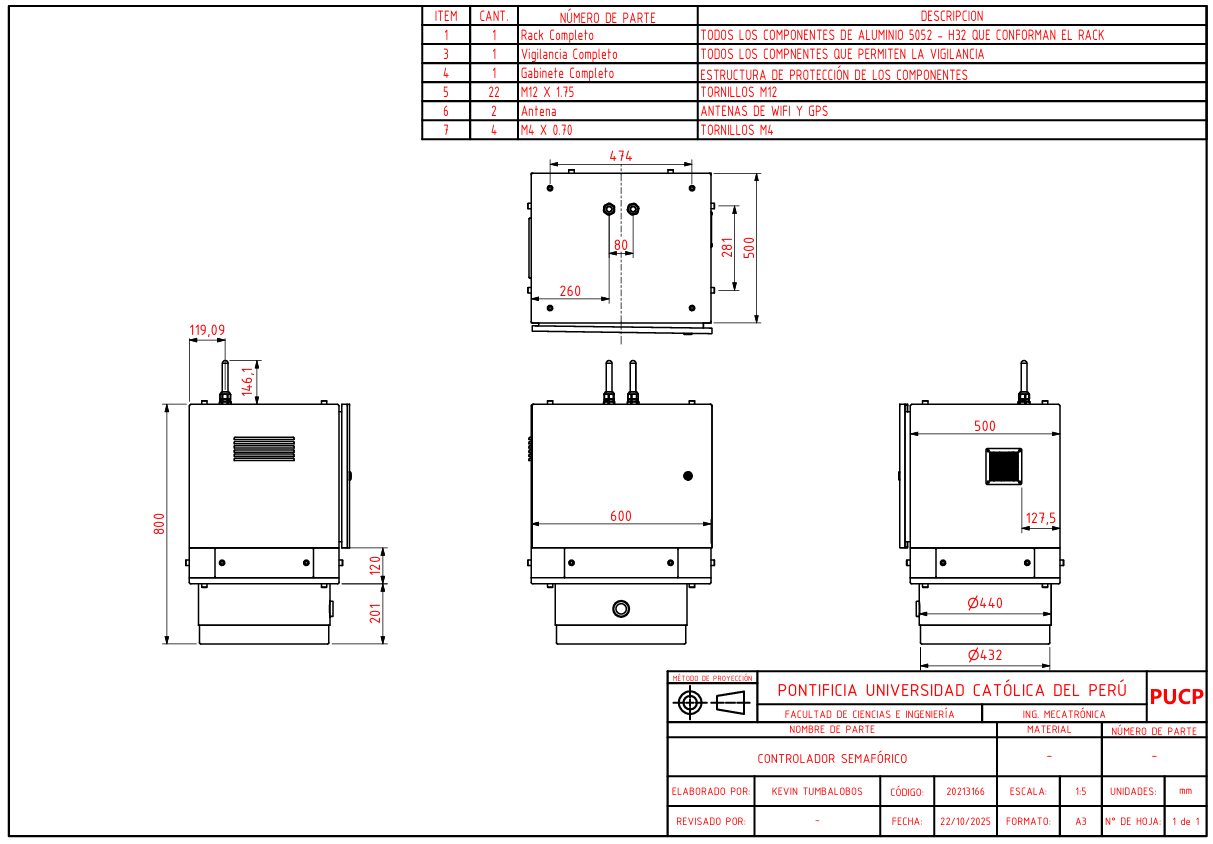
\includegraphics[width=0.92\linewidth,height=0.62\textheight,keepaspectratio]{./media/image3.png}
\end{center}

\textbf{SECCIÓN E:}

\begin{center}
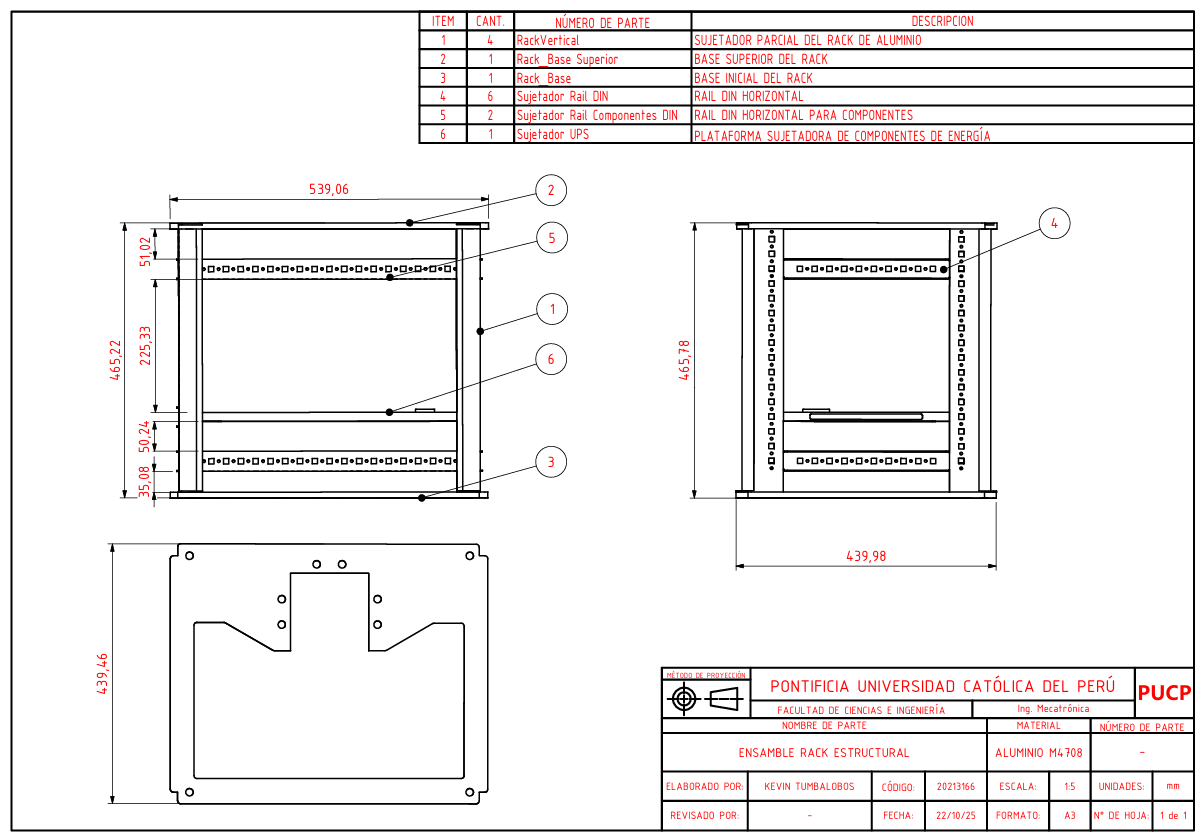
\includegraphics[width=0.92\linewidth,height=0.62\textheight,keepaspectratio]{./media/image138.png}
\end{center}

\begin{center}
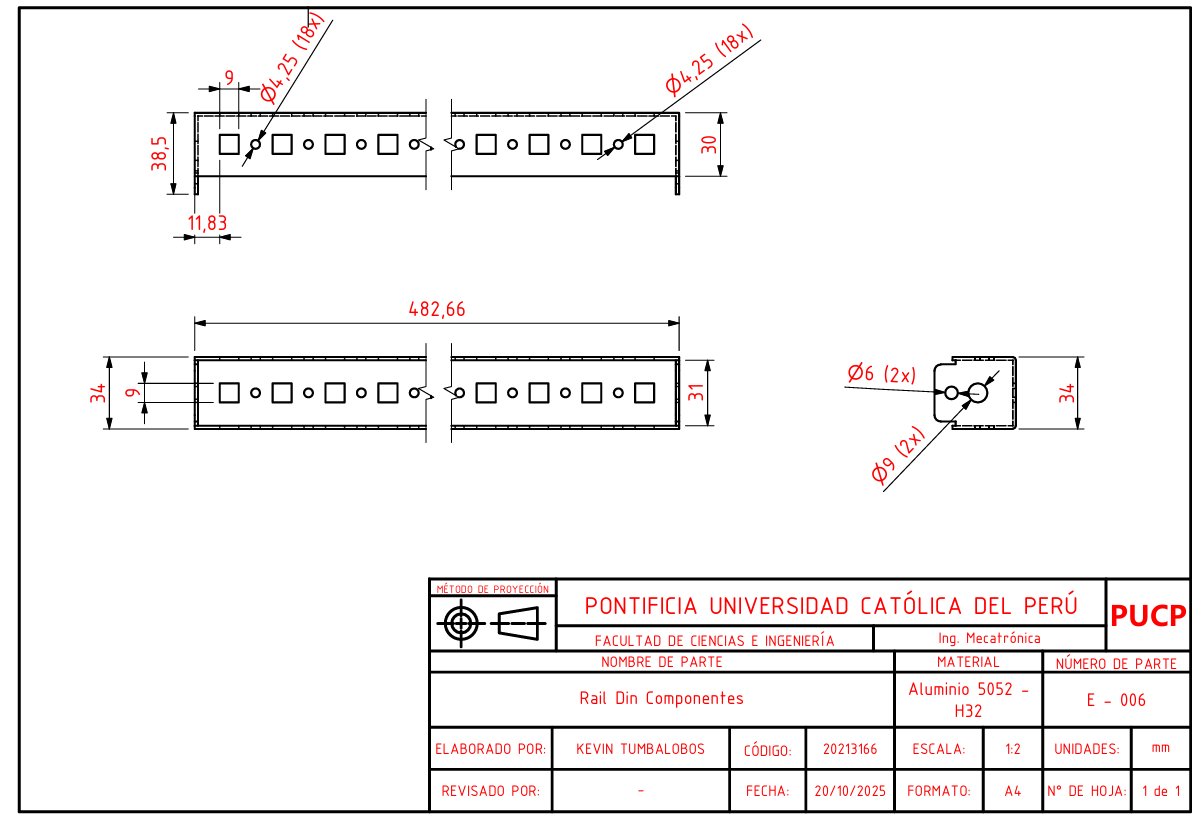
\includegraphics[width=0.92\linewidth,height=0.62\textheight,keepaspectratio]{./media/image94.png}
\end{center}

\begin{center}
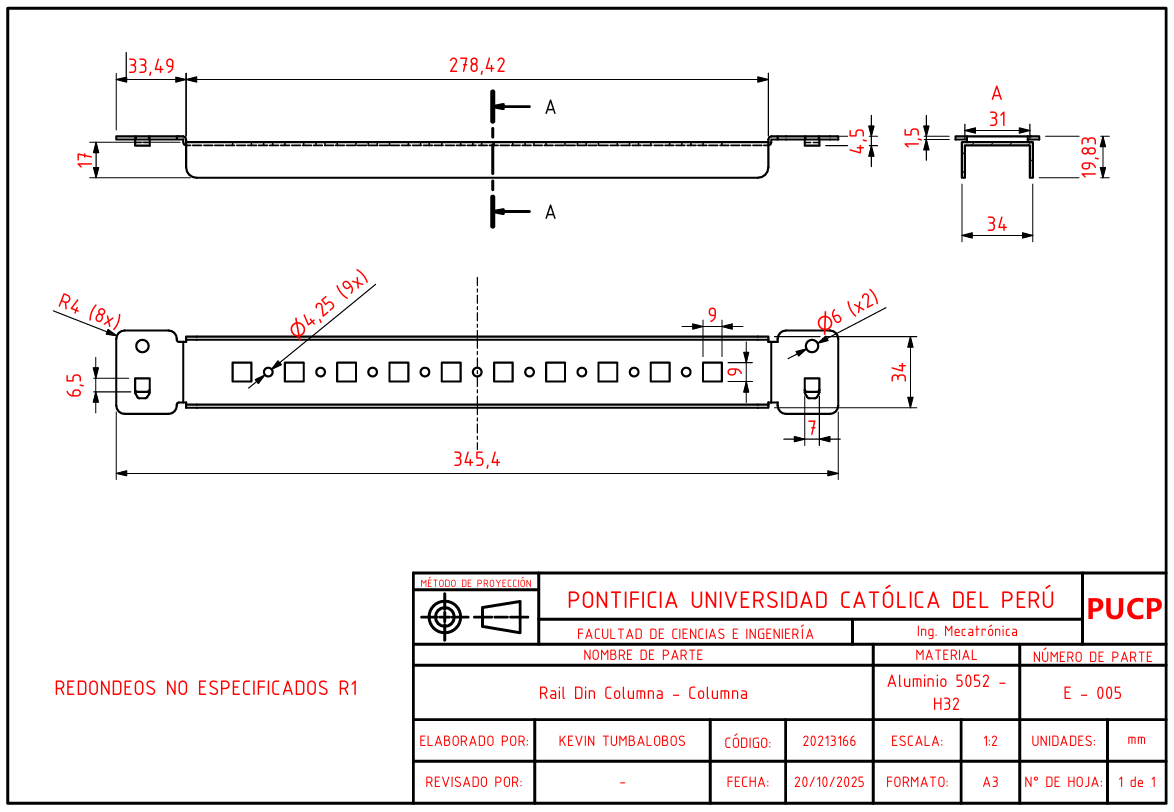
\includegraphics[width=0.92\linewidth,height=0.62\textheight,keepaspectratio]{./media/image62.png}
\end{center}

\begin{center}
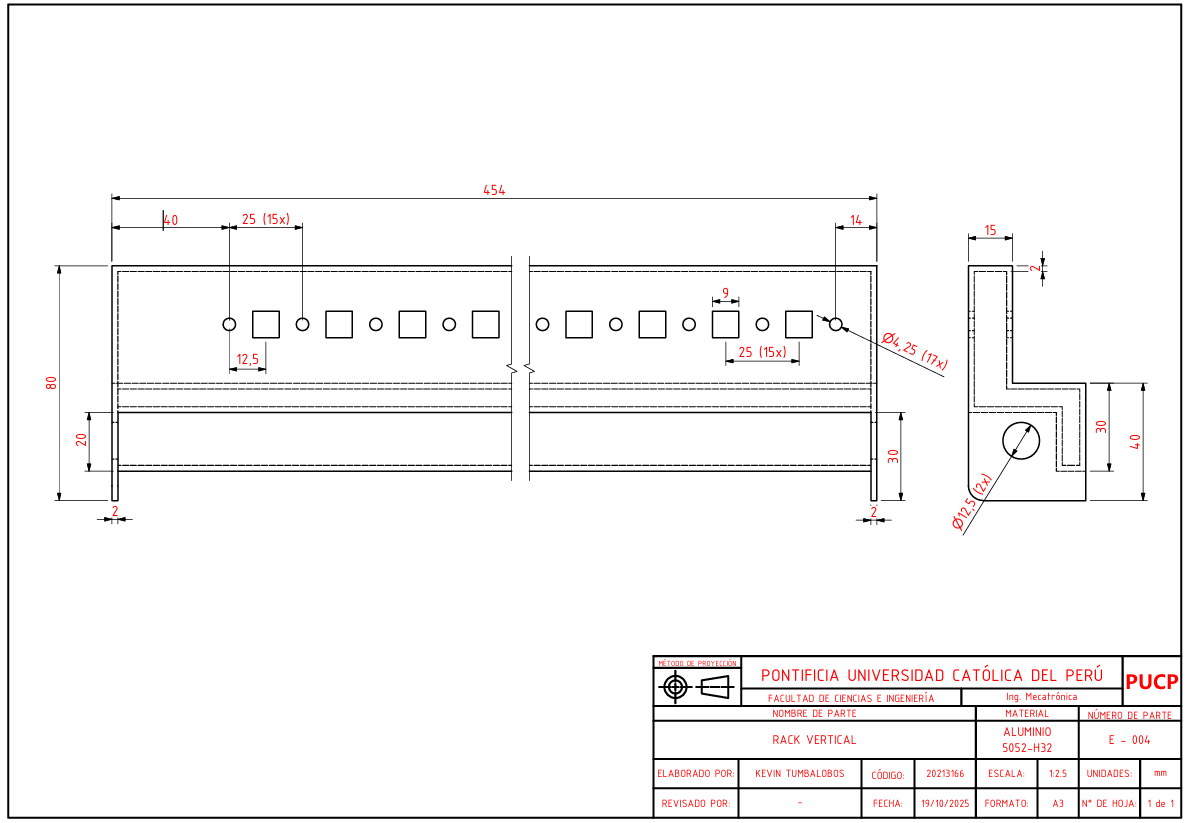
\includegraphics[width=0.92\linewidth,height=0.62\textheight,keepaspectratio]{./media/image137.png}
\end{center}\begin{center}
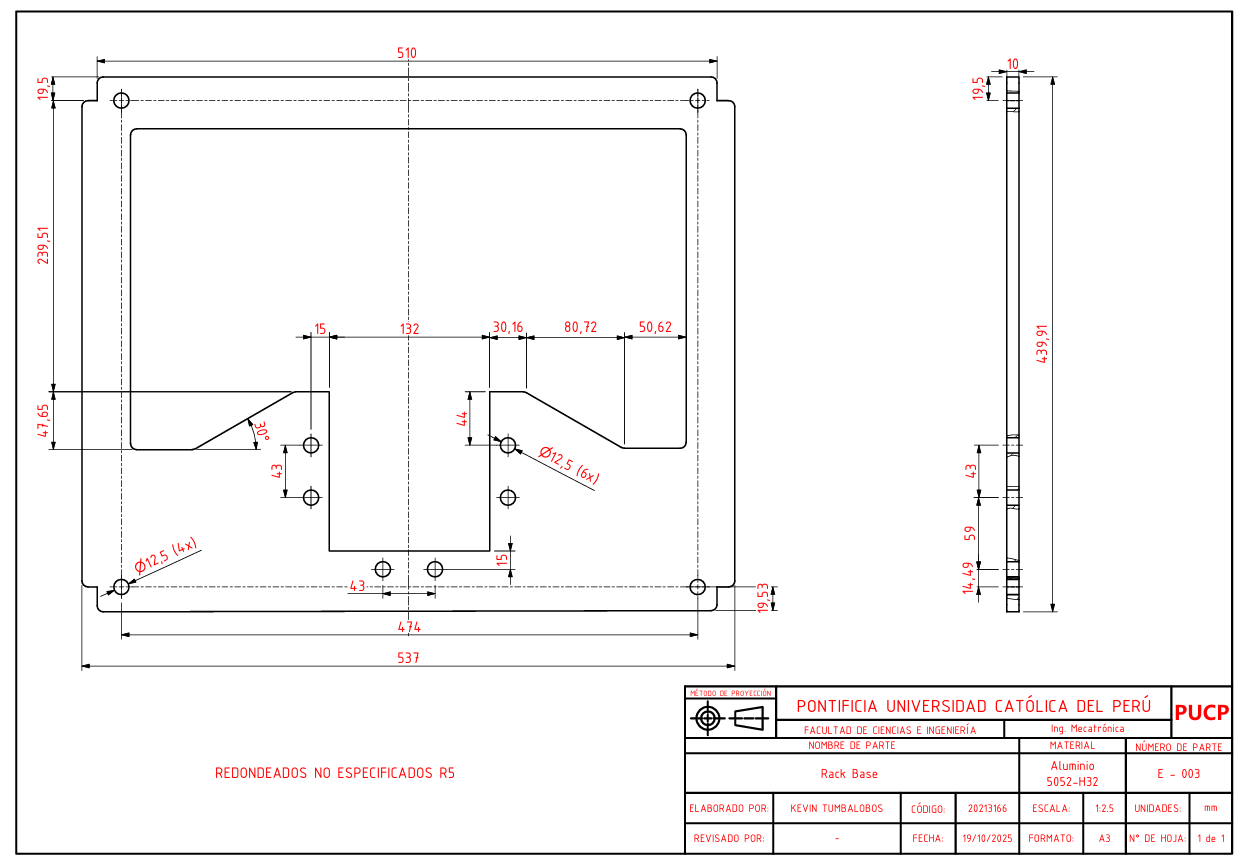
\includegraphics[width=0.92\linewidth,height=0.62\textheight,keepaspectratio]{./media/image32.png}
\end{center}\begin{center}
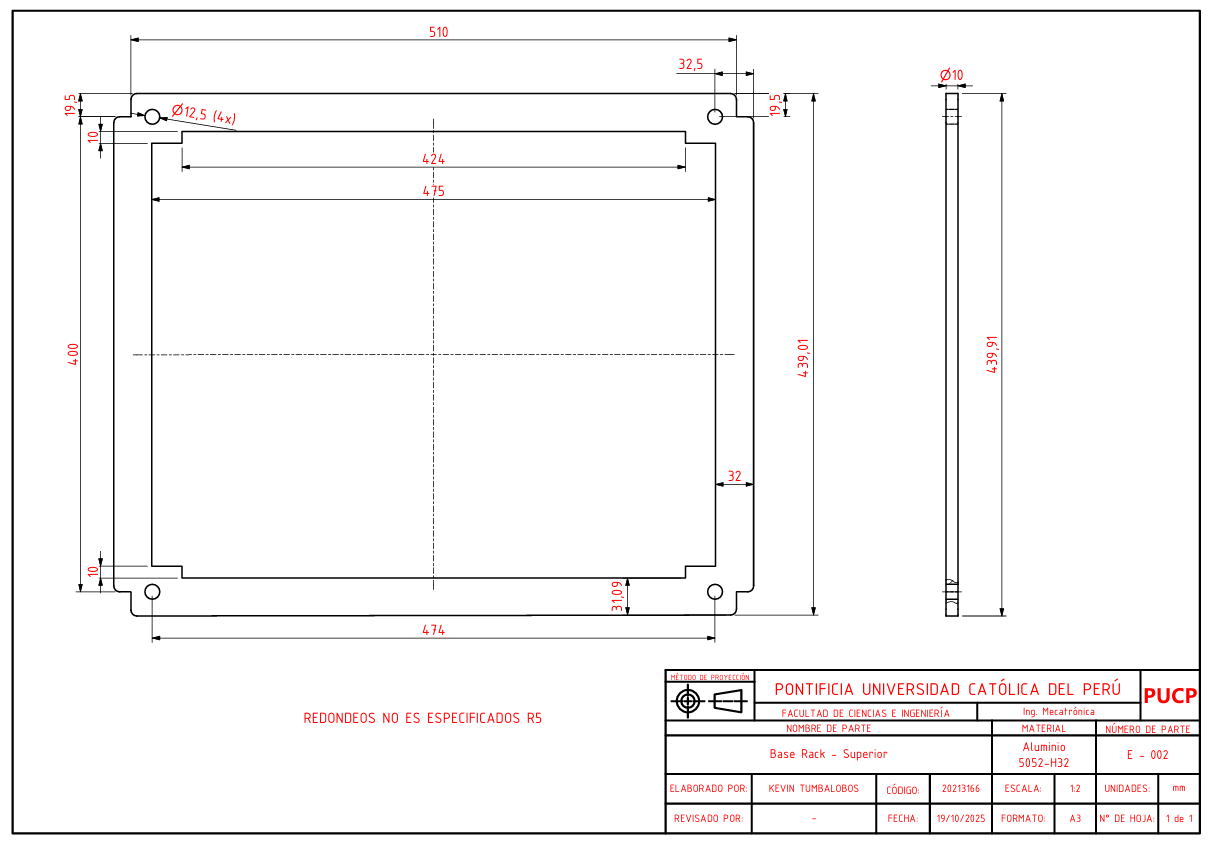
\includegraphics[width=0.92\linewidth,height=0.62\textheight,keepaspectratio]{./media/image121.png}
\end{center}\begin{center}
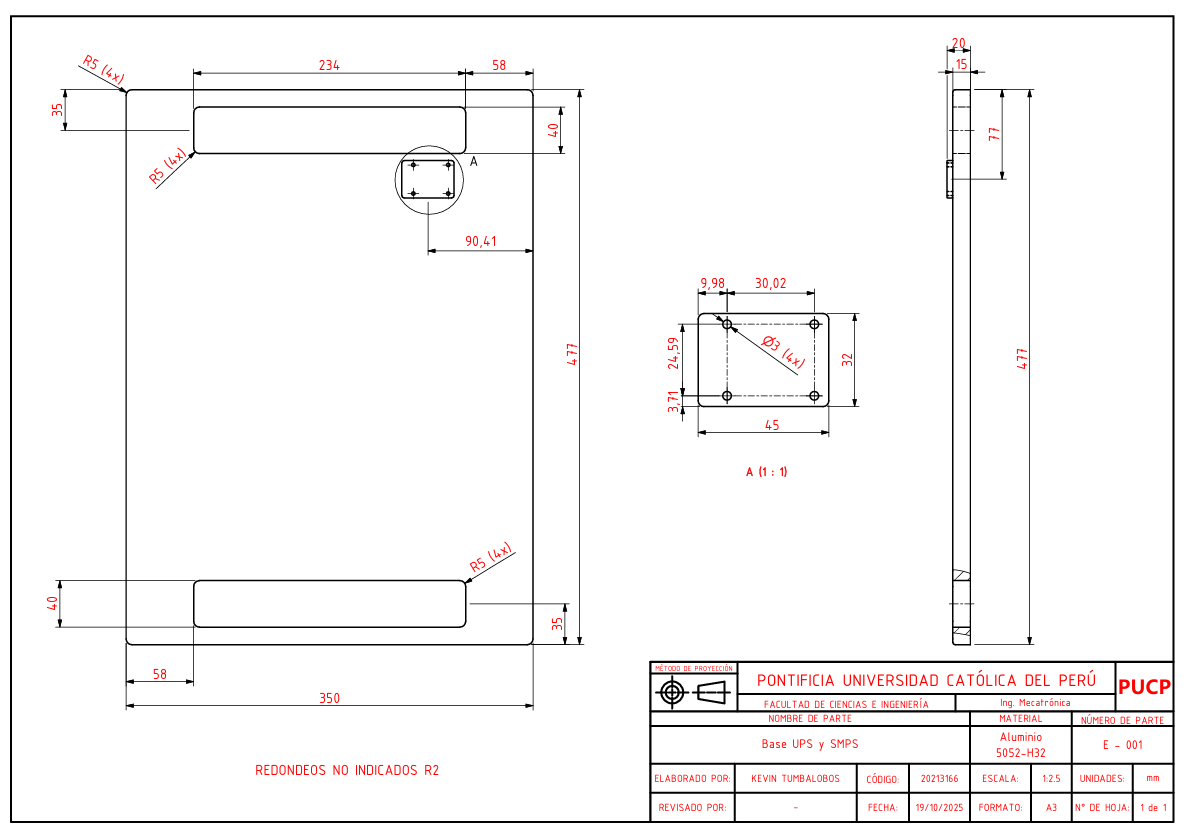
\includegraphics[width=0.92\linewidth,height=0.62\textheight,keepaspectratio]{./media/image59.png}
\end{center}

\textbf{SECCIÓN G:}

\begin{center}
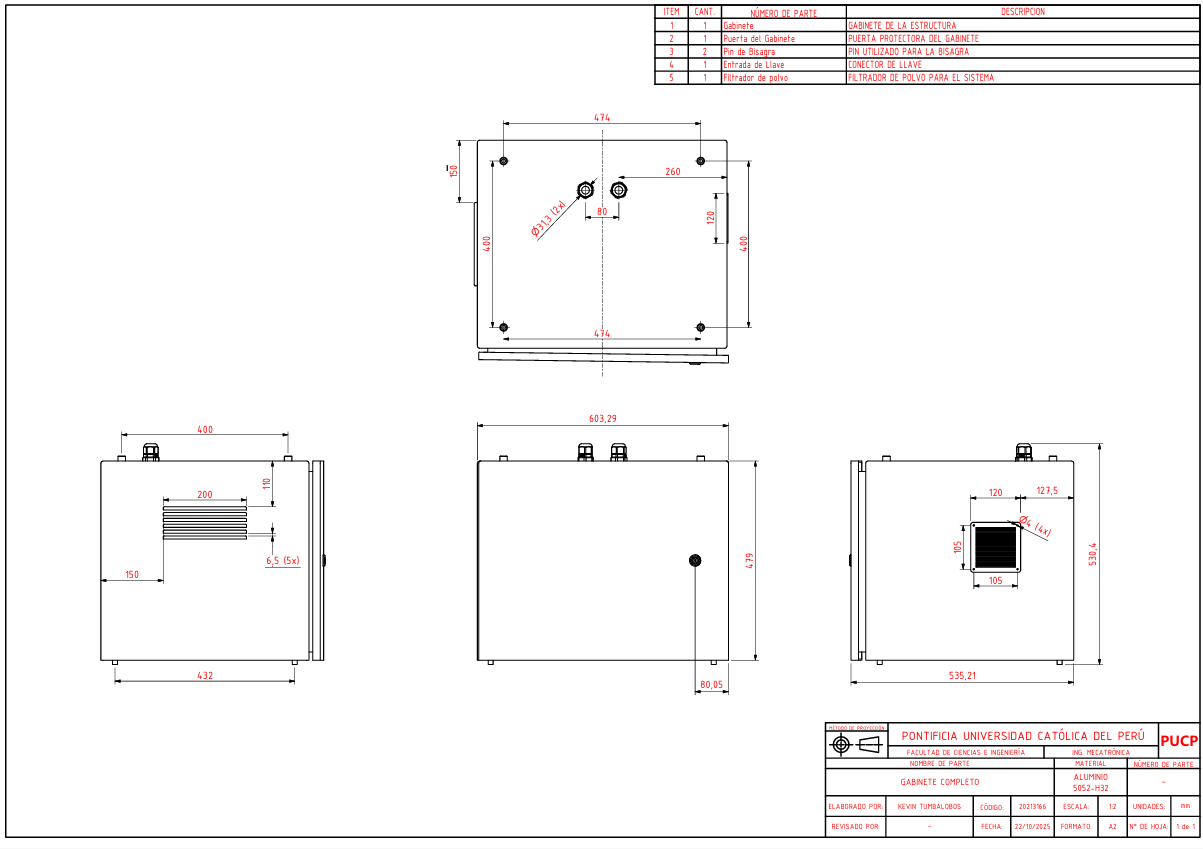
\includegraphics[width=0.92\linewidth,height=0.62\textheight,keepaspectratio]{./media/image34.png}
\end{center}\begin{center}
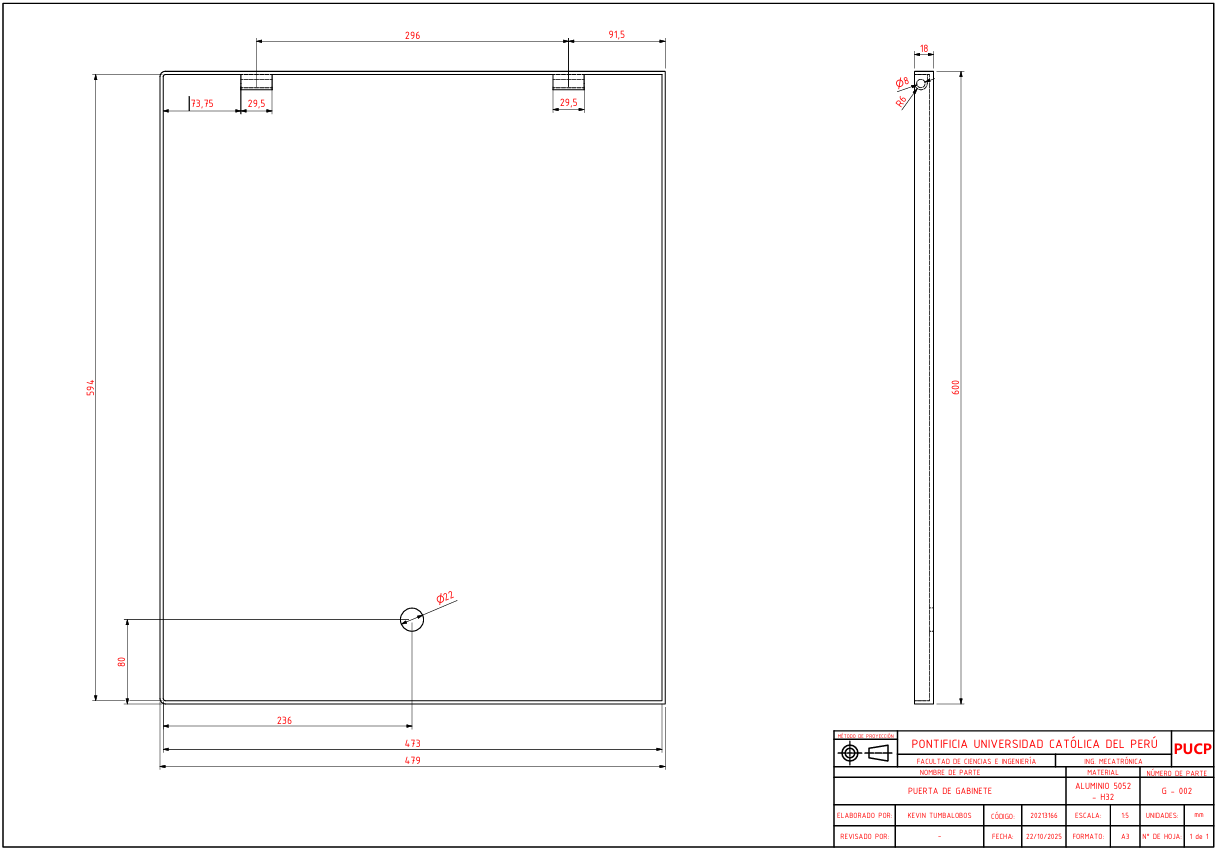
\includegraphics[width=0.92\linewidth,height=0.62\textheight,keepaspectratio]{./media/image23.png}
\end{center}\begin{center}
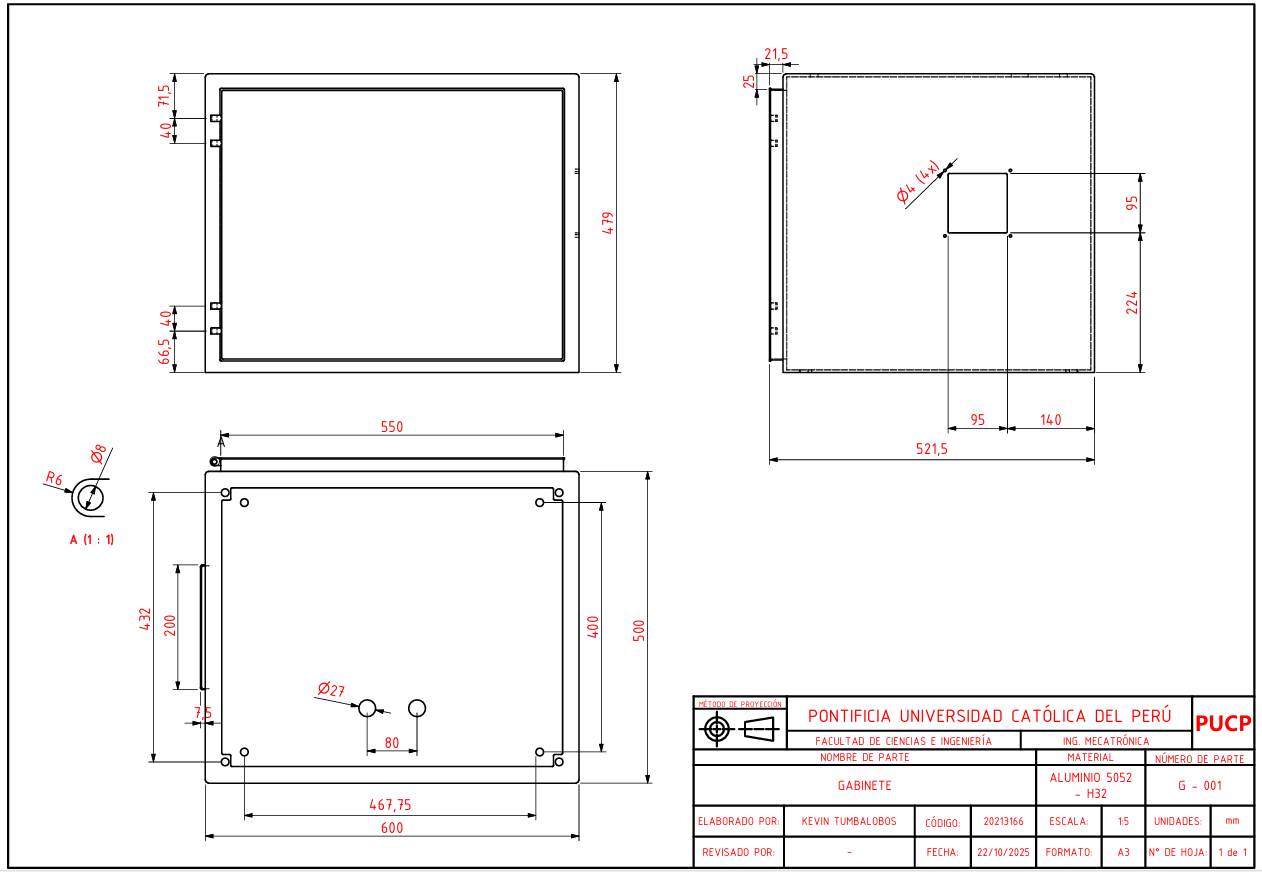
\includegraphics[width=0.92\linewidth,height=0.62\textheight,keepaspectratio]{./media/image142.png}
\end{center}

\textbf{SECCIÓN M:}

\begin{center}
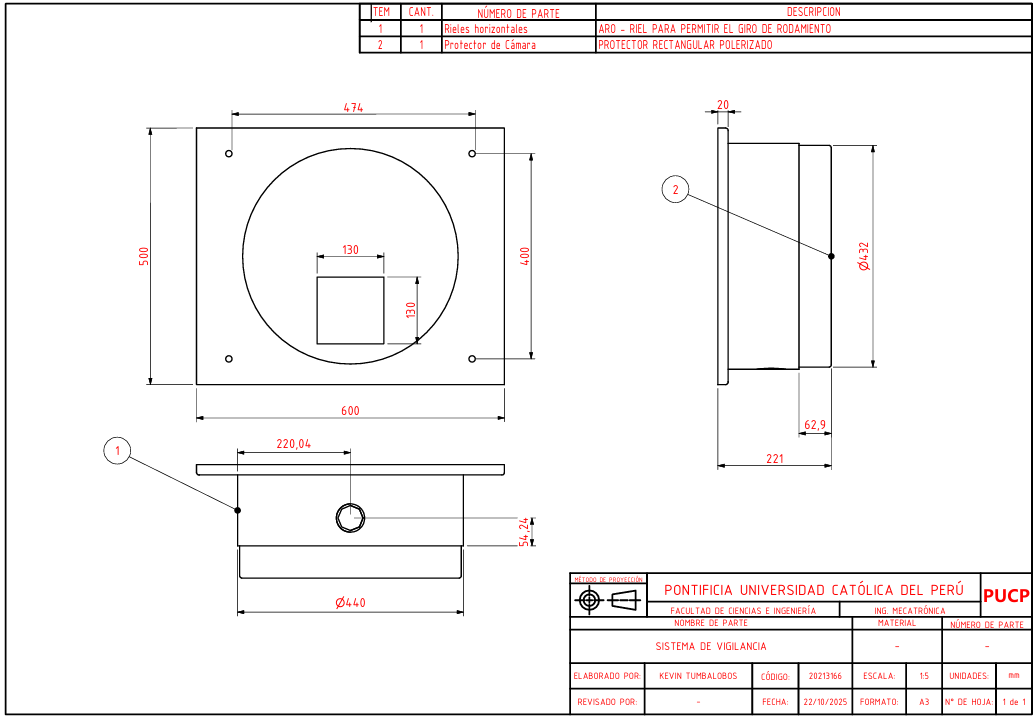
\includegraphics[width=0.92\linewidth,height=0.62\textheight,keepaspectratio]{./media/image135.png}
\end{center}\begin{center}
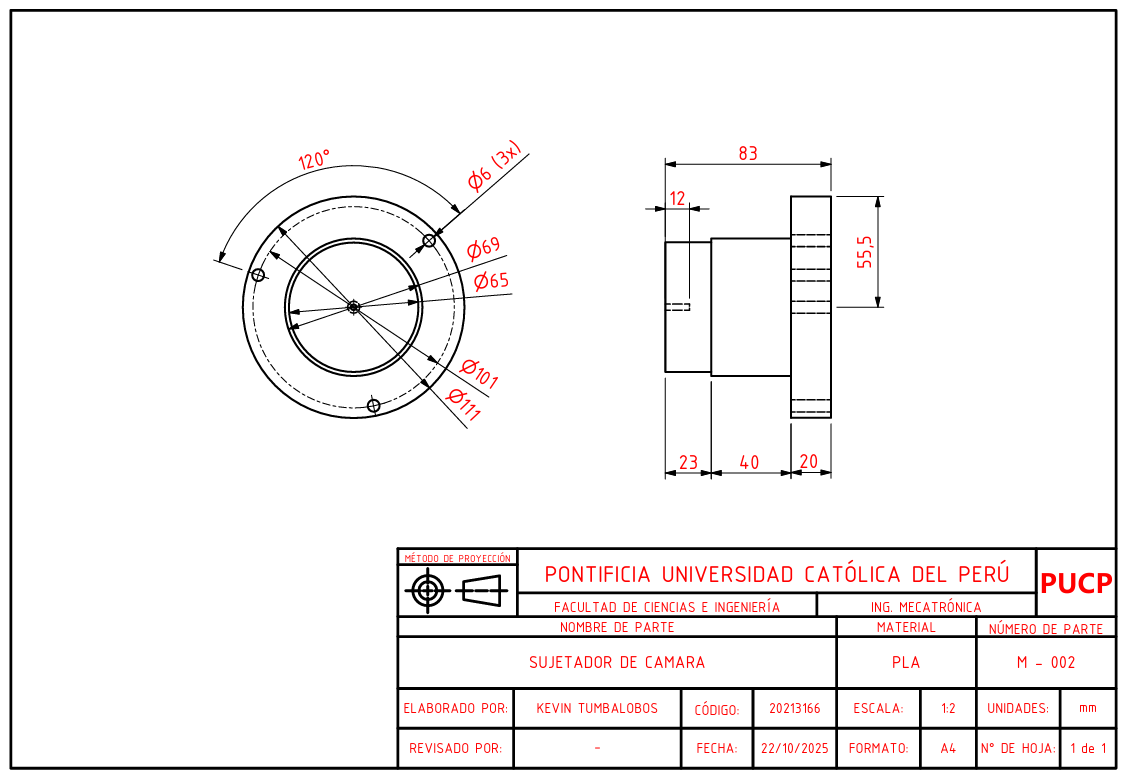
\includegraphics[width=0.92\linewidth,height=0.62\textheight,keepaspectratio]{./media/image98.png}
\end{center}\begin{center}
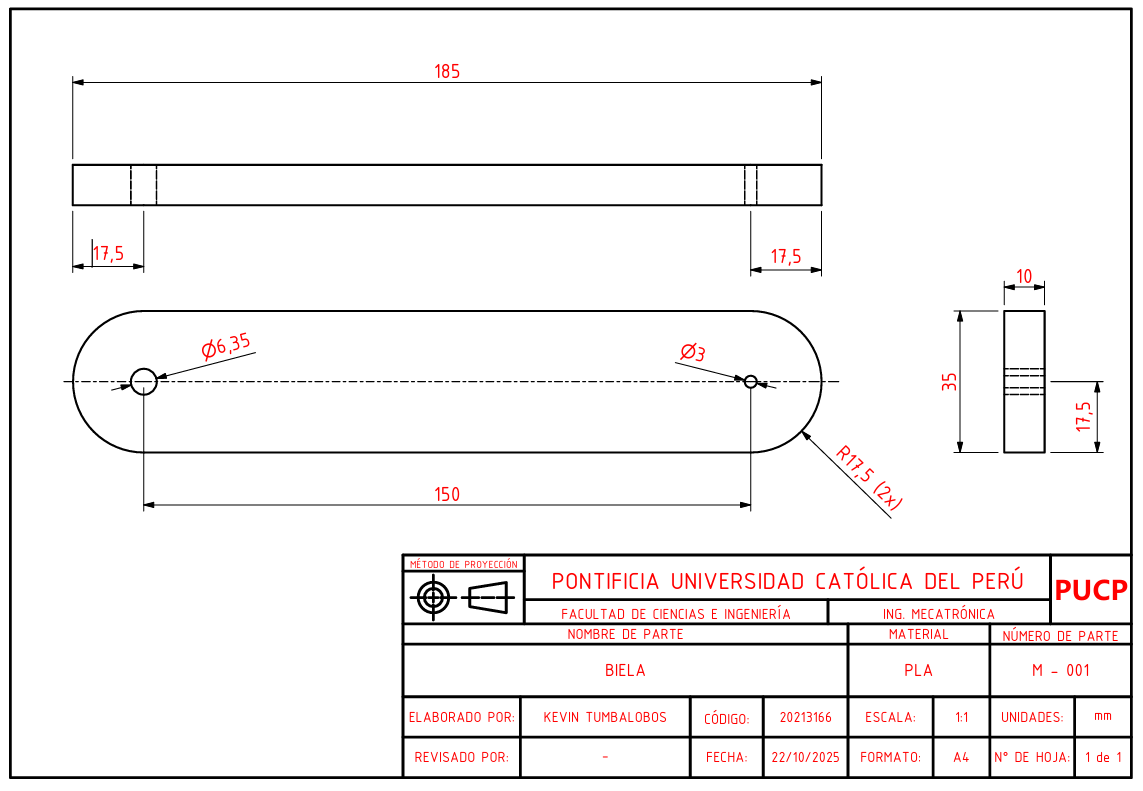
\includegraphics[width=0.92\linewidth,height=0.62\textheight,keepaspectratio]{./media/image38.png}
\end{center}\begin{center}
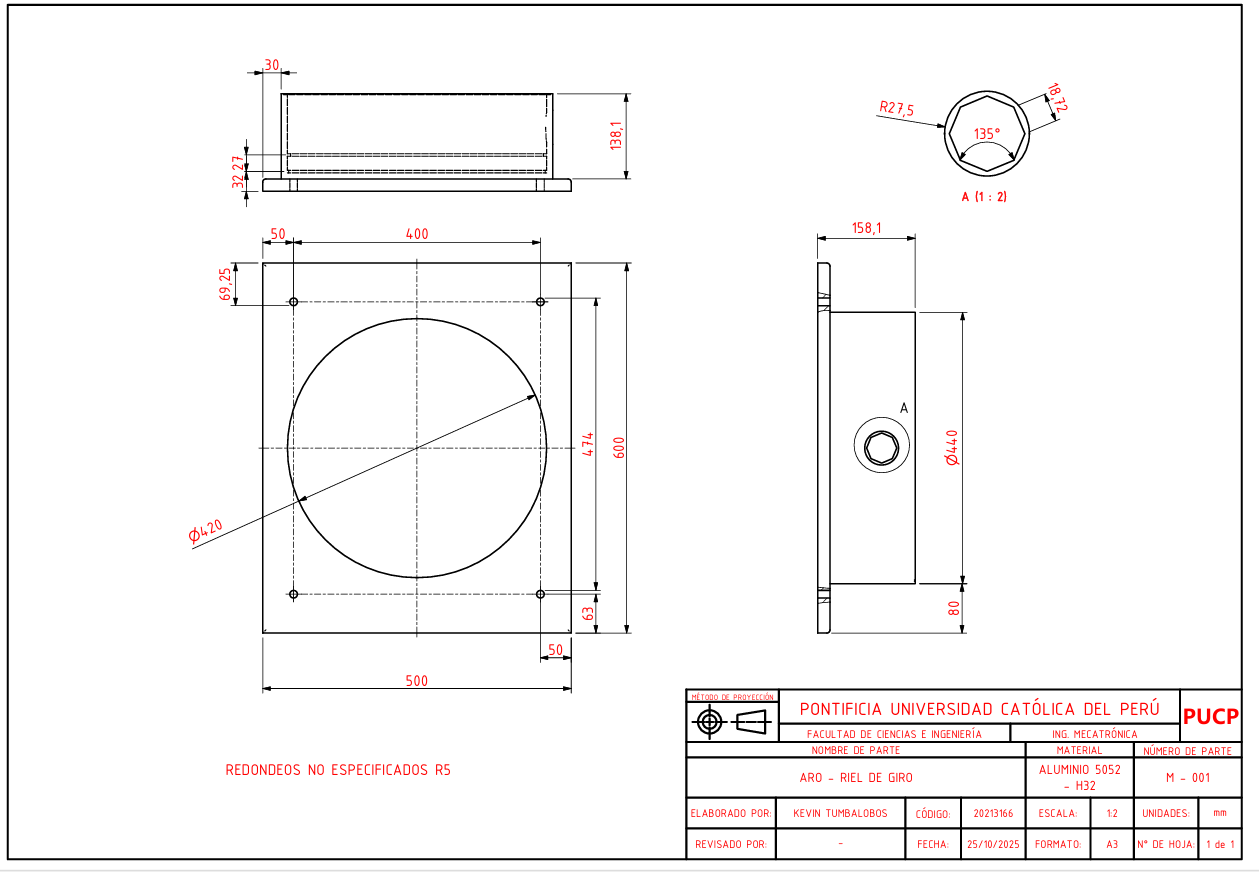
\includegraphics[width=0.92\linewidth,height=0.62\textheight,keepaspectratio]{./media/image119.png}
\end{center}

\textbf{SECCIÓN V:}

\begin{center}
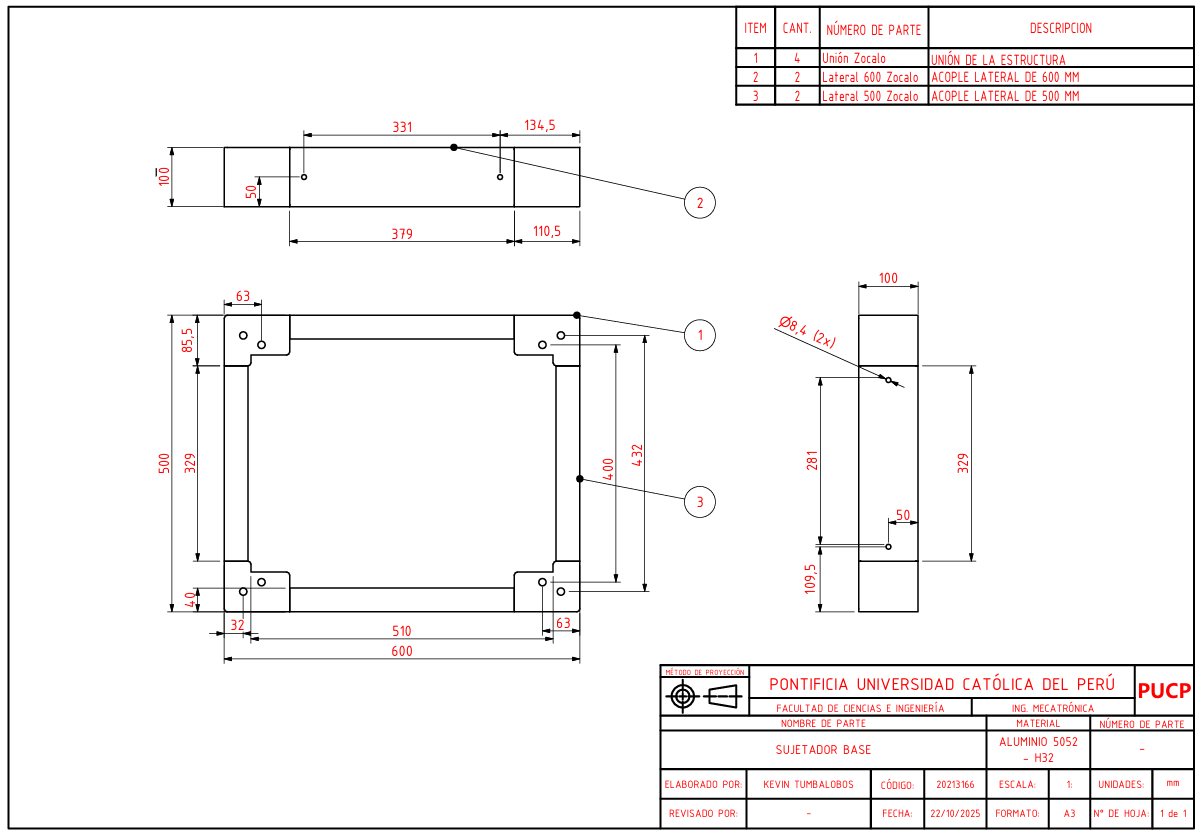
\includegraphics[width=0.92\linewidth,height=0.62\textheight,keepaspectratio]{./media/image123.png}
\end{center}\begin{center}
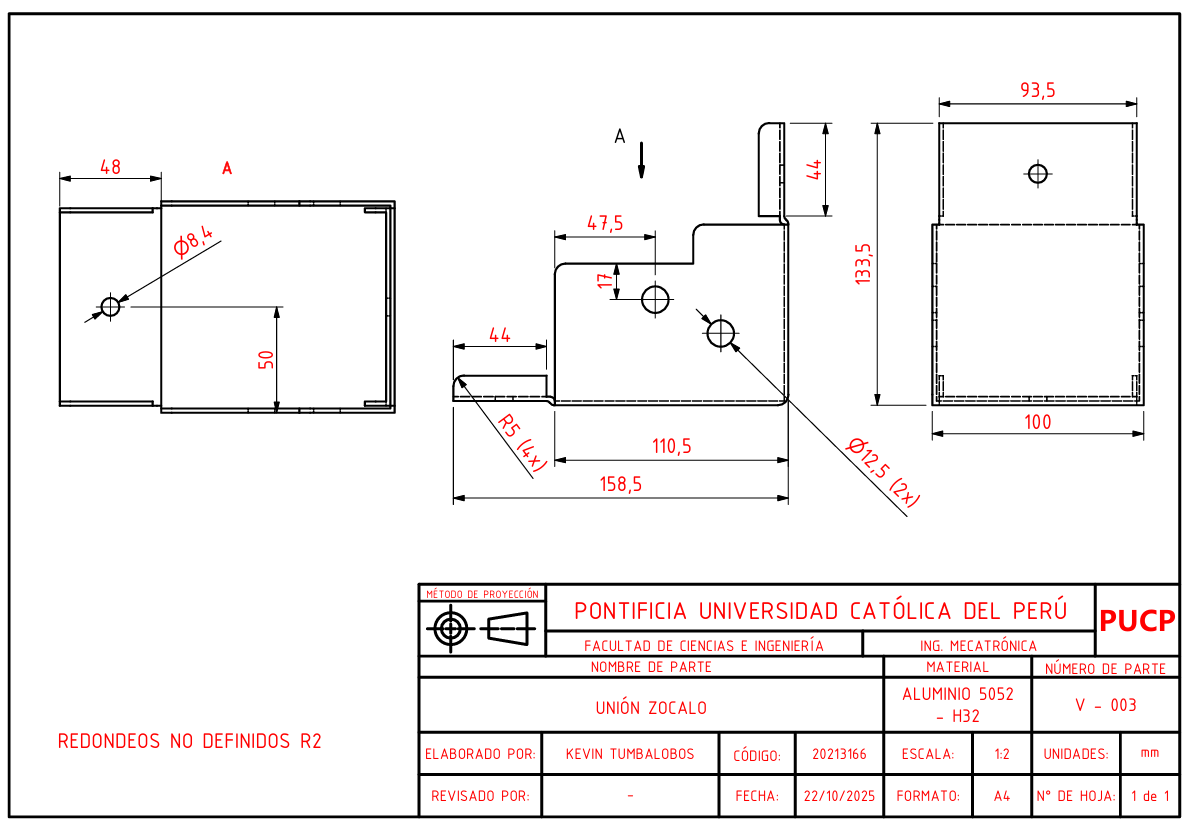
\includegraphics[width=0.92\linewidth,height=0.62\textheight,keepaspectratio]{./media/image63.png}
\end{center}\begin{center}
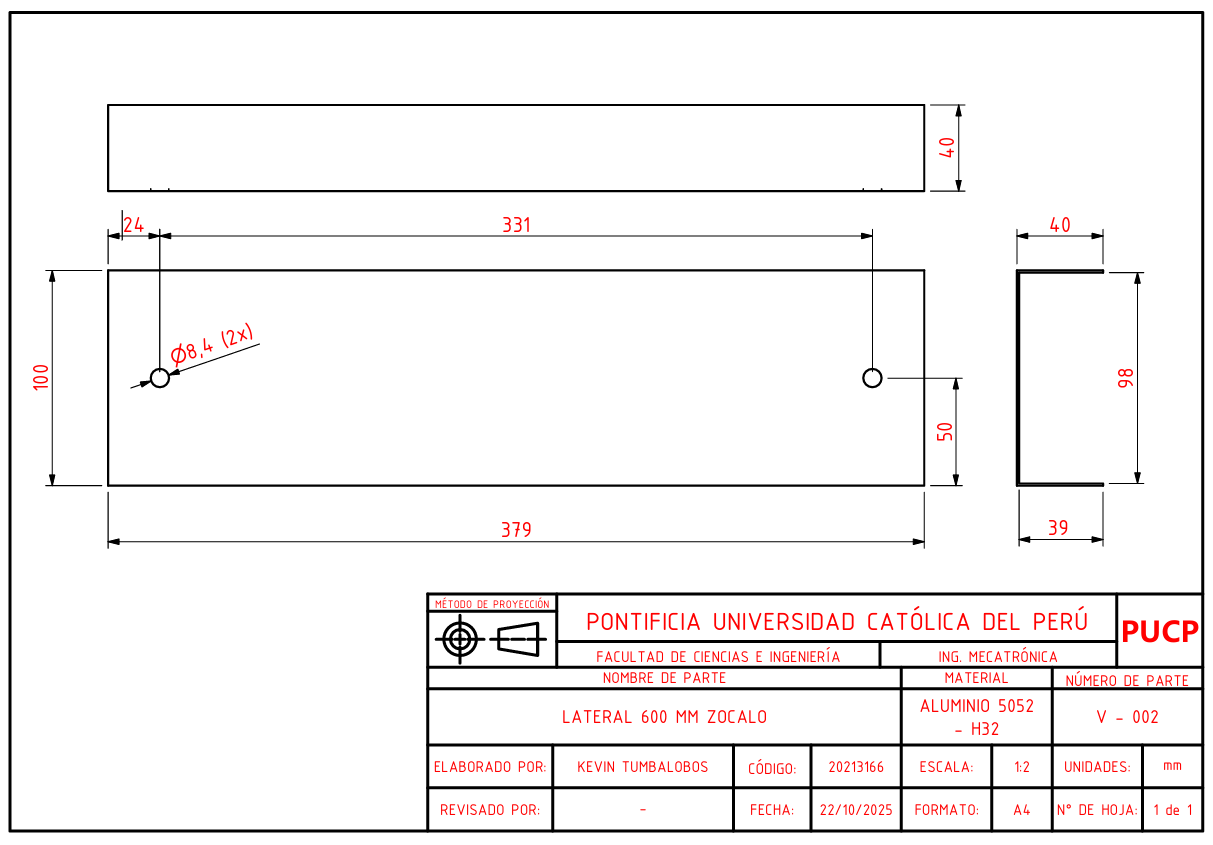
\includegraphics[width=0.92\linewidth,height=0.62\textheight,keepaspectratio]{./media/image92.png}
\end{center}\begin{center}
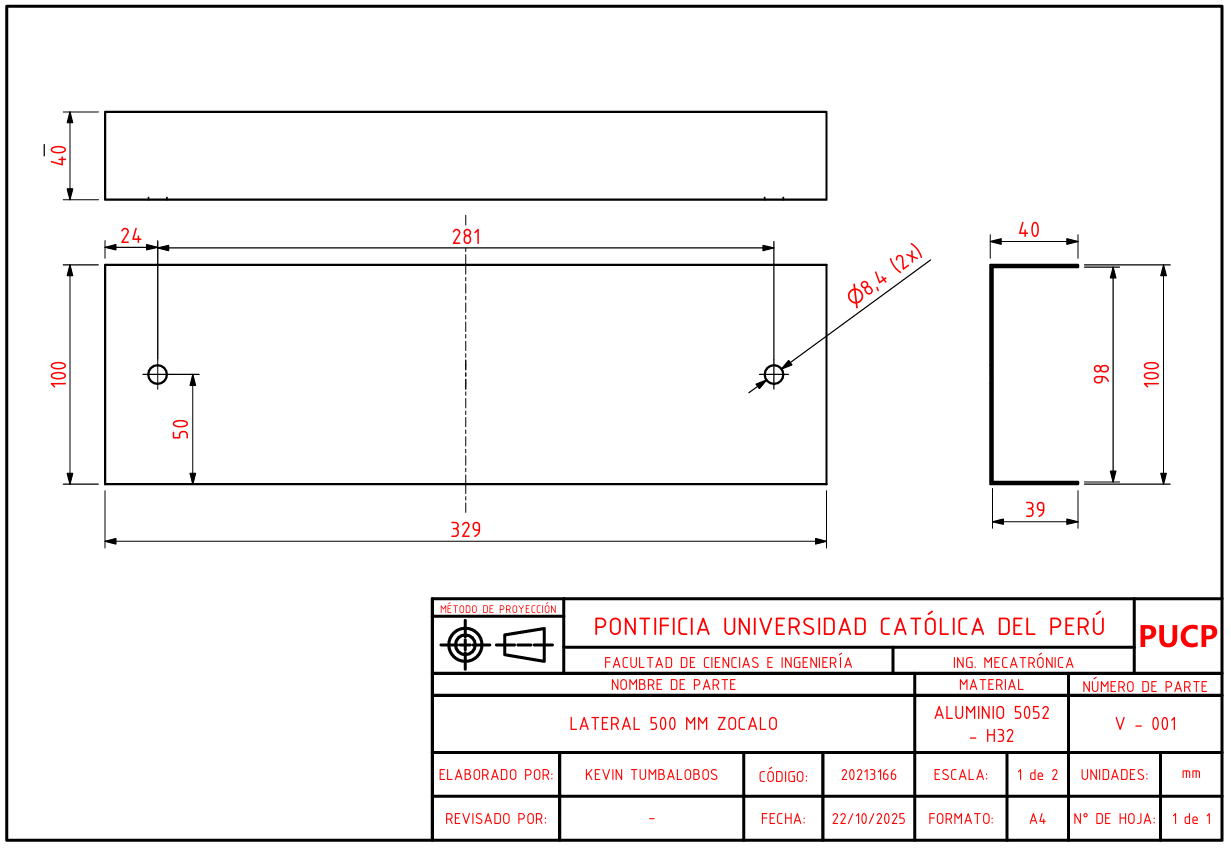
\includegraphics[width=0.92\linewidth,height=0.62\textheight,keepaspectratio]{./media/image4.png}
\end{center}

\textbf{SECCIÓN P:}

\begin{center}
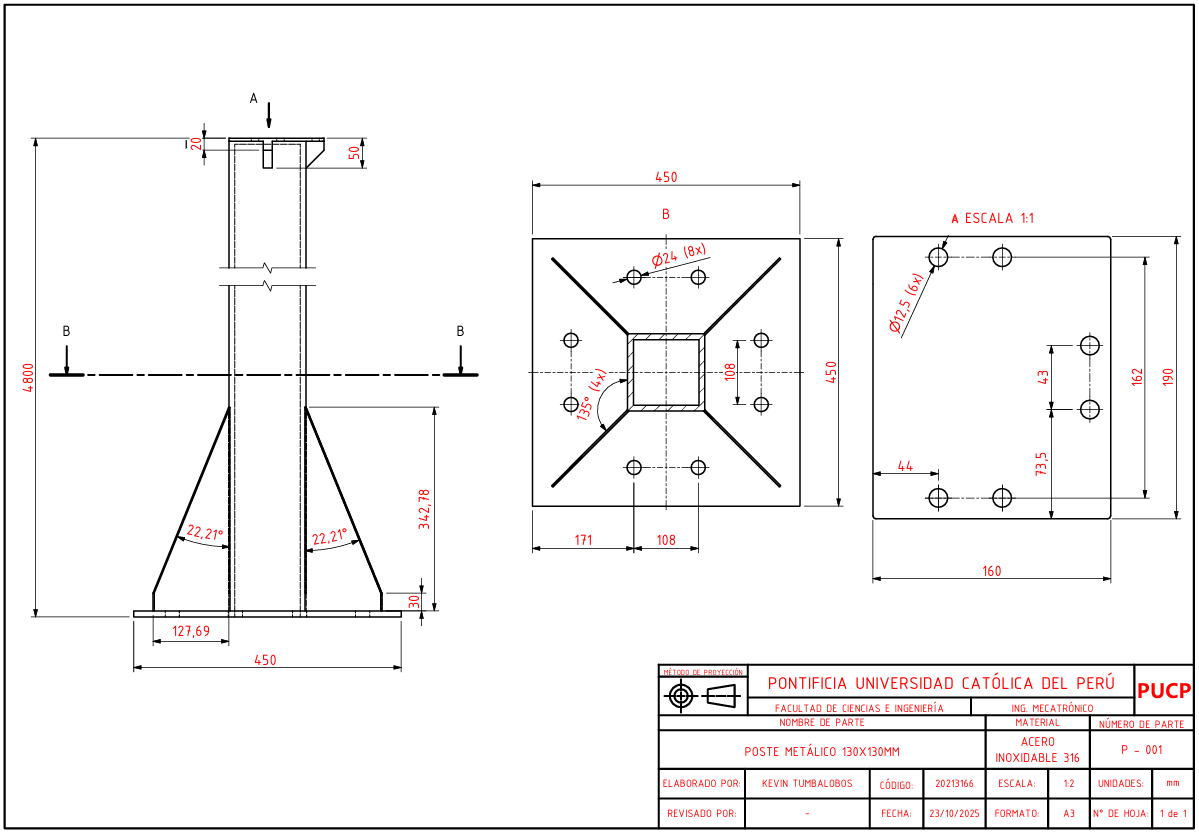
\includegraphics[width=0.92\linewidth,height=0.62\textheight,keepaspectratio]{./media/image129.png}
\end{center}

\textbf{SECCIÓN Z:}

\begin{center}
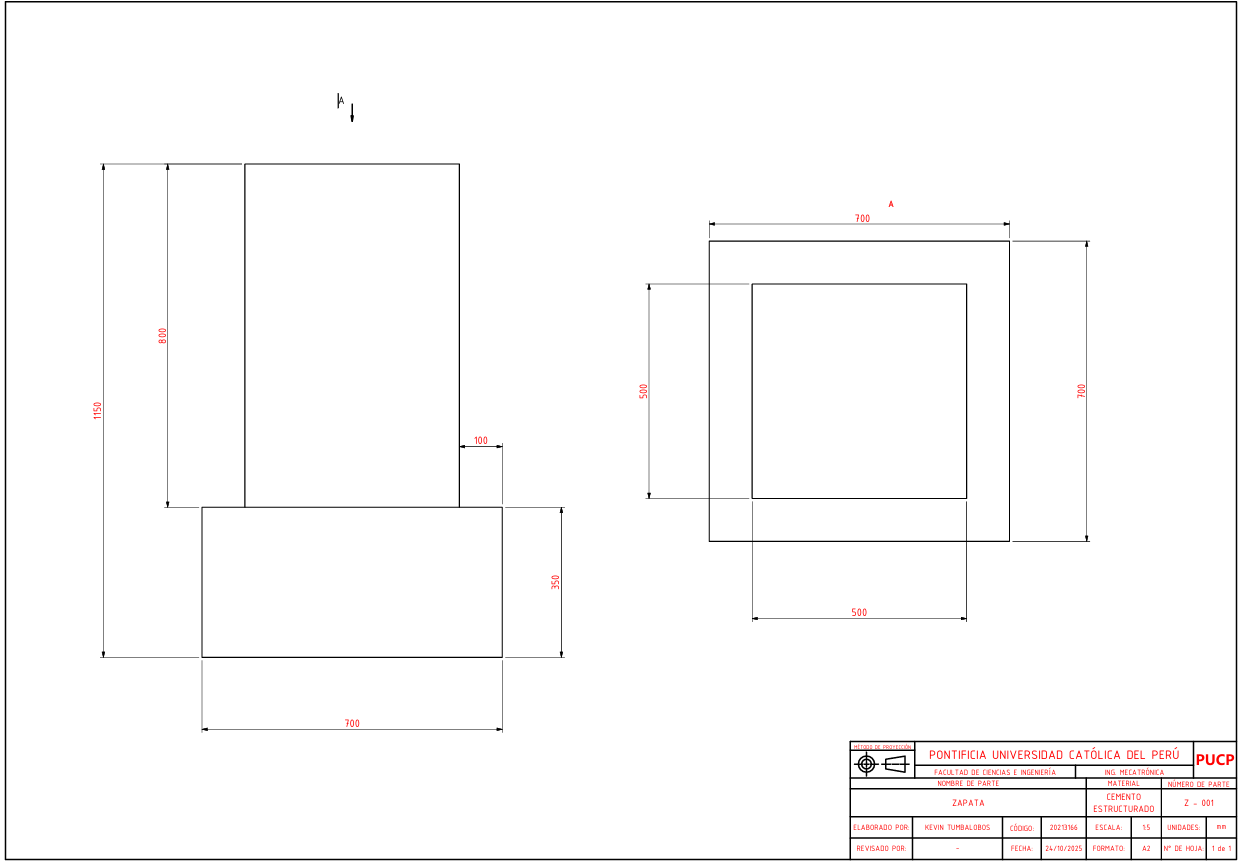
\includegraphics[width=0.92\linewidth,height=0.62\textheight,keepaspectratio]{./media/image106.png}
\end{center}


\end{document}
